\documentclass[12pt, openany]{book}
\usepackage{comment}
\specialcomment{answer}{\textbf{Answer: }}{}

%Change below to decide whether answers are displayed in the text

%Decide whether to show answers:
%Hides the answers to short answer questions
\excludecomment{answer}
%Shows multiple choice answers
%\newcommand{\correct}{\textbf{(Correct)}}
%Hides multiple choice answers
\newcommand{\correct}{}


%\usepackage{animate} %to animate images
\usepackage{mathtools} % for \Aboxed
\usepackage{paralist}
\usepackage{calc}
\usepackage{subfig}
\usepackage{setspace}
\usepackage{amssymb}
\usepackage{amsmath}
\usepackage{amstext}
\usepackage[font={small,it}]{caption}
\usepackage[pdftex]{graphicx} %Does not work in pressbooks!!!
\usepackage{fancyhdr,lastpage}
\usepackage{url}
\usepackage{longtable}
\usepackage{comment}
\usepackage{ifthen}
\usepackage{color}
\usepackage[colorlinks=true,linkcolor=blue,urlcolor=blue]{hyperref}
\usepackage[explicit]{titlesec}
\usepackage{lmodern}
\usepackage{listings}
\usepackage{parskip}
\usepackage[table]{xcolor}
%\usepackage{enumitem}
\usepackage{wrapfig}
\usepackage[framemethod=TikZ]{mdframed}
\usepackage{titlesec} %for spacing around titles
\usepackage{caption}
\usepackage[separate-uncertainty = true]{siunitx}
\usepackage{float}
\restylefloat{table}
\usepackage{multicol}
\usepackage[shortlabels]{enumitem}
%\lstset{language=Python,showstringspaces=false,commentstyle=} 
\usepackage{tikz}
\usepackage[american,smartlabels]{circuitikz}%for drawing circuits

\usetikzlibrary{arrows}

%%Some math and other shortcuts
\newcommand{\chloe}{Chlo\"e~}
\newcommand{\die}[2]{\frac{\partial #1}{\partial #2}}
\newcommand{\ddt}{\frac{d}{dt}}
\newcommand{\lagd}{\mathcal{L}}
\newcommand{\code}[1]{\texttt{#1}}
\newcommand{\angstrom}{\textup{\AA}}
\newcommand{\ampere}{Amp\`ere}
\newcommand{\amperesp}{Amp\`ere~}

\newcommand{\pvec}[1]{\vec{#1}\mkern2mu\vphantom{#1}} % for a vector of a primed quantity, e.g. \vec p ', should be \pvec p'

%Colours
\definecolor{mygreen}{rgb}{0.2,0.6,0}
\definecolor{TBgreen}{rgb}{0.0,0.5,0.0}
\definecolor{TBblue}{rgb}{0.0, 0.58, 0.71}
\definecolor{TBred}{rgb}{0.8, 0.25, 0.33}
\definecolor{TBorange}{rgb}{0.89, 0.35, 0.13}
\definecolor{TBPurple}{rgb}{0.6,0.4,0.8}

%Stuff for writing code:

\lstset{ %
  belowskip=0pt,
  aboveskip=0pt,
  caption=\relax,
  backgroundcolor=\color{white},   % choose the background color; you must add \usepackage{color} or \usepackage{xcolor}
  basicstyle=\footnotesize,        % the size of the fonts that are used for the code
  breakatwhitespace=false,         % sets if automatic breaks should only happen at whitespace
  breaklines=true,                 % sets automatic line breaking
  captionpos=t,                    % sets the caption-position to bottom
  commentstyle=\color{mygreen},    % comment style
  deletekeywords={...},            % if you want to delete keywords from the given language
  escapeinside={(*}{*)},          % if you want to add LaTeX within your code
  extendedchars=true,              % lets you use non-ASCII characters; for 8-bits encodings only, does not work with UTF-8
  frame=none,	                   % adds a frame around the code
  keepspaces=true,                 % keeps spaces in text, useful for keeping indentation of code (possibly needs columns=flexible)
  keywordstyle=\color{blue},       % keyword style
  language=Python,                 % the language of the code
  otherkeywords={*,...},           % if you want to add more keywords to the set
  numbers=none,                    % where to put the line-numbers; possible values are (none, left, right)
  numbersep=5pt,                   % how far the line-numbers are from the code
  numberstyle=\tiny\color{black}, % the style that is used for the line-numbers
  rulecolor=\color{black},         % if not set, the frame-color may be changed on line-breaks within not-black text (e.g. comments (green here))
  showspaces=false,                % show spaces everywhere adding particular underscores; it overrides 'showstringspaces'
  showstringspaces=false,          % underline spaces within strings only
  showtabs=false,                  % show tabs within strings adding particular underscores
  stepnumber=1,                    % the step between two line-numbers. If it's 1, each line will be numbered
  stringstyle=\color{red},     % string literal style
  tabsize=2,	                   % sets default tabsize to 2 spaces
  title=\lstname                   % show the filename of files included with \lstinputlisting; also try caption instead of title
}

%Environments for writing code
\DeclareCaptionFont{white}{\color{white}}
\DeclareCaptionFormat{listing}{\colorbox{gray}{\parbox{\textwidth}{#1#2#3}}}
  
\captionsetup[lstlisting]{format=listing,labelfont=white,textfont=white}
\renewcommand{\lstlistingname}{Python Example}
\renewcommand{\lstlistlistingname}{List of \lstlistingname s}

\lstnewenvironment{python}[1][]{
  \lstset{#1, language=Python}%
  \renewcommand\lstlistingname{Python Code}
}{}

\lstnewenvironment{poutput}{
 \lstset{caption=\mbox{}, language=,aboveskip=-3pt}
 \addtocounter{lstlisting}{-1}
 \renewcommand\lstlistingname{Output}
}{}


%%Pretty chapter headings:
\newlength\chapnumb
\setlength\chapnumb{4cm}

\titleformat{\chapter}[block]
{\normalfont\sffamily}{}{0pt}
{\parbox[b]{\chapnumb}{%
   \fontsize{120}{110}\selectfont\thechapter}%
  \parbox[b]{\dimexpr\textwidth-\chapnumb\relax}{%
    \raggedleft%
    \hfill{\LARGE#1}\\
    \rule{\dimexpr\textwidth-\chapnumb\relax}{0.4pt}}}
\titleformat{name=\chapter,numberless}[block]
{\normalfont\sffamily}{}{0pt}
{\parbox[b]{\chapnumb}{%
   \mbox{}}%
  \parbox[b]{\dimexpr\textwidth-\chapnumb\relax}{%
    \raggedleft%
    \hfill{\LARGE#1}\\
    \rule{\dimexpr\textwidth-\chapnumb\relax}{0.4pt}}}


%%%spacing around titles
%\setlength{\parindent}{0pt}
%\parskip = \baselineskip

%spacing around captions (e.g. caption after a table)
\captionsetup{belowskip=6pt,aboveskip=4pt}

\titlespacing*{\chapter}
{0pt}{25ex}{20ex}
\titlespacing*{\section}
{0pt}{1ex}{1.5ex}
\titlespacing*{\subsection}
{0pt}{1ex}{1.5ex}
\titlespacing*{\subsubsection}
{0pt}{1ex}{1.5ex}

%%% Spacing in lists:
\setlist{nosep}

%%Verticall spacing between table rows
\renewcommand{\arraystretch}{1.5}

\setlength{\intextsep}{12pt}

%space before itemized list:
%\setlength{\topsep}{-10pt} %does nothing?

%%Simplifed figure environment:

\newenvironment{capfig}[3]{\begin{center}\includegraphics[width=#1]{#2}\captionof{figure}{#3}\end{center}}{}


%Wrap figure environments (right or left). Argument #1 (default value 12, specified as optional), is the number of 
%lines that the figure should take.
%space around wrap figures:
%\setlength{\intextsep}{20pt}%
%\setlength{\columnsep}{5pt}%
\newenvironment{Rwcapfig}[4][0]{
\begingroup
%\setlength{\intextsep}{0pt}%
\setlength{\columnsep}{10pt}%
\begin{wrapfigure}[#1]{R}{#2}\centering\includegraphics[width=#2]{#3}\caption{#4}\end{wrapfigure}}{\endgroup}

\newenvironment{rwcapfig}[4][0]{
\begingroup
%\setlength{\intextsep}{0pt}%
\setlength{\columnsep}{10pt}%
\begin{wrapfigure}[#1]{r}{#2}\centering\includegraphics[width=#2]{#3}\caption{#4}\end{wrapfigure}}{\endgroup}

\newenvironment{Lwcapfig}[4][0]{
\begingroup
%\setlength{\intextsep}{0pt}%
\setlength{\columnsep}{10pt}%
\begin{wrapfigure}[#1]{L}{#2}\centering\includegraphics[width=#2]{#3}\caption{#4}\end{wrapfigure}}{\endgroup }


\newenvironment{lwcapfig}[4][0]{
\begingroup
%\setlength{\intextsep}{0pt}%
\setlength{\columnsep}{10pt}%
\begin{wrapfigure}[#1]{l}{#2}\centering\includegraphics[width=#2]{#3}\caption{#4}\end{wrapfigure}}{\endgroup }

\newenvironment{lwfig}[3][0]{
\begingroup
\setlength{\intextsep}{0pt}%
\setlength{\columnsep}{10pt}%
\begin{wrapfigure}[#1]{l}{#2}\centering\includegraphics[width=#2]{#3}\end{wrapfigure}}{\endgroup }

%Environments (in the works) %%%%%%%%%%%%%%%%%%%%%%%%%%%%%%%%%%%%%%%%%%%%%%%%%%%%%%%%%%%%%%%%%%%%%%%%%%%%%%%%%%%%%%%%%%%%%%%%%%%%%%%%%%%%%%%%%%%%%%%%%%%%%%%%%%%%%%%%%%%%%%%%%%%%%%%
%% Environments to Keep
%%Learning Objectives:
\newenvironment{learningObjectives}[1]{%
\mdfsetup{%
    frametitle={%
        \tikz[baseline=(current bounding box.east),outer sep=0pt]
        \node[anchor=west,rectangle,fill=TBblue, minimum width=5cm, rounded corners=0.2cm]
        {\strut Learning Object
        ives};},
    frametitlefont=\color{white}\sffamily\bfseries,
    innertopmargin=0pt,linecolor=TBblue,%
    linewidth=1pt,topline=true,%
    frametitleaboveskip=\dimexpr-\ht\strutbox\relax%
}
\vspace{10pt}
\begin{mdframed}\begin{itemize}[label=\textcolor{TBblue}{\textbullet}] #1 \end{itemize}}{\end{mdframed}}


%%Opening Question:
\newenvironment{opening}[1]{%
\mdfsetup{%
    frametitle={%
        \tikz[baseline=(current bounding box.east),outer sep=0pt]
        \node[anchor=west,rectangle,fill=TBblue, minimum width=5cm,rounded corners=0.2cm]
        {\strut Think About It};},
    frametitlefont=\color{white}\sffamily\bfseries,
    innertopmargin=0pt,linecolor=TBblue,backgroundcolor=TBblue!5,%
    linewidth=1pt,topline=true,%
    frametitleaboveskip=\dimexpr-\ht\strutbox\relax%
}
\vspace{10pt}
\begin{mdframed}[nobreak=true]\relax #1}{%
\end{mdframed}}

%Problems
\newcounter{problem}[chapter]
\def\theproblem{\thechapter-\arabic{problem}}

\newenvironment{problem}[2]
  {\refstepcounter{problem}\textbf{Problem \theproblem: }#2 (\hyperref[#1]{Solution})} %
  {\vspace{2ex}}
  
\newenvironment{problemParts}[2]
  {\refstepcounter{problem}\textbf{Problem \theproblem: }#2 (\hyperref[#1]{Solution}) %
  \begin{enumerate}[label=\alph*),topsep=-10pt]}%
   {\end{enumerate}}
  {\vspace{2ex}}
  
\newenvironment{MCquestion}[1]{#1%
   \begin{enumerate}[label=\Alph*),topsep=-10pt]}{%
   \end{enumerate}}

%Example Box with counter  
\newcounter{example}[chapter]
\def\theexample{\thechapter-\arabic{example}}
\newenvironment{example}[2]{% 
\refstepcounter{example}%
\mdfsetup{%
    frametitle={% 
        \tikz[baseline=(current bounding box.east),outer sep=0pt]
        \node[anchor=west,rectangle,fill=TBred, minimum width=5cm,rounded corners=0.2cm]
        {\strut Example~\theexample};},
    frametitlefont=\color{white}\sffamily\bfseries,
    skipabove=\strutbox,
    innertopmargin={0.5cm},
    linecolor=TBred,%
    linewidth=1pt,topline=true,%
    frametitleaboveskip=\dimexpr-\ht\strutbox\relax%
    %frametitleaboveskip=-\strutbox
}
\begin{mdframed}[]\relax #1 \leavevmode \\ \newline { \color{TBred}\textsf{\large Solution}} \\ {\color{TBred}\rule[10pt]{\textwidth}{1pt}} \\ #2}{%
\end{mdframed}}

%Review Box
\newenvironment{review}[1]{%
\mdfsetup{%
    frametitle={%
        \tikz[baseline=(current bounding box.east),outer sep=0pt]
        \node[anchor=west,rectangle,fill=TBorange, minimum width=5cm,rounded corners=0.2cm]
        {\strut Review Topics};},
    frametitlefont=\color{white}\sffamily\bfseries,
    innertopmargin=0pt,linecolor=TBorange,backgroundcolor=TBorange!5,%
    linewidth=1pt,topline=true,%
    frametitleaboveskip=\dimexpr-\ht\strutbox\relax%
}
\vspace{10pt}
\begin{mdframed}[nobreak=true]\relax #1}{%
\end{mdframed}}

%Reflect and Research
\newenvironment{chapteractivity}[2]{%
\mdfsetup{%
    frametitle={%
        \tikz[baseline=(current bounding box.east),outer sep=0pt]
        \node[anchor=west,rectangle,fill=TBgreen!80, minimum width=5cm,rounded corners=0.2cm]
        {\strut #1};},
    frametitlefont=\color{white}\sffamily\bfseries,
    innertopmargin=0pt,linecolor=TBgreen!80,backgroundcolor=TBgreen!5,%
    linewidth=1pt,topline=true,%
    frametitleaboveskip=\dimexpr-\ht\strutbox\relax%
}
\vspace{10pt}
\begin{mdframed}\begin{enumerate}[itemsep=1ex] #2
   \end{enumerate}}
{\end{mdframed}}



%%Checkpoint question in a box, with counter:
\newcounter{checkpoint}[chapter]
\def\thecheckpoint{\thechapter-\arabic{checkpoint}}

\newenvironment{checkpoint}[1]{%
\refstepcounter{checkpoint}%
\mdfsetup{%
    frametitle={%
        \tikz[baseline=(current bounding box.east),outer sep=0pt]
        \node[anchor=west,rectangle,fill=TBgreen!80, minimum width=5cm,rounded corners=0.2cm]
        {\strut Checkpoint~\thecheckpoint};},
    frametitlefont=\color{white}\sffamily\bfseries,
    innertopmargin=0pt,linecolor=TBgreen!80,backgroundcolor=TBgreen!5,%
    linewidth=1pt,topline=true,%
    frametitleaboveskip=\dimexpr-\ht\strutbox\relax%
}
\vspace{10pt}
\begin{mdframed}[nobreak=true]\relax #1}{%
\end{mdframed}}


%Student Opinion with option for student name
\newenvironment{studentOpinion}[2]{%
\mdfsetup{%
    frametitle={%
        \tikz[baseline=(current bounding box.east),outer sep=0pt]
        \node[anchor=west,rectangle,fill=TBorange, minimum width=5cm,rounded corners=0.2cm]
        {\strut #1's Thoughts};},
    frametitlefont=\color{white}\sffamily\bfseries,
    linecolor=TBorange,%
    linewidth=1pt,topline=true,
    skipabove=\strutbox,
    innertopmargin={0.5cm},%
    frametitleaboveskip=\dimexpr-\ht\strutbox\relax%
}
\vspace{10pt}
\begin{mdframed}[]\relax #2}{%
\end{mdframed}}

%%Important Equations:
\newenvironment{importantEquations}[1]{%
\mdfsetup{%
    frametitle={%
        \tikz[baseline=(current bounding box.east),outer sep=0pt]
        \node[anchor=west,rectangle,fill=TBblue, minimum width=5cm,rounded corners=0.2cm]
        {\strut Important Equations};},
    frametitlefont=\color{white}\sffamily\bfseries,
    innertopmargin=0pt,linecolor=TBblue,%
    linewidth=1pt,topline=true,%
    frametitleaboveskip=\dimexpr-\ht\strutbox\relax%
}
\vspace{10pt}
\begin{mdframed}[nobreak=false]\relax #1}{%
\end{mdframed}}

%%Definitions
\newenvironment{definitions}[1]{%
	\mdfsetup{%
		frametitle={%
			\tikz[baseline=(current bounding box.east),outer sep=0pt]
			\node[anchor=west,rectangle,fill=TBPurple, minimum width=5cm,rounded corners=0.2cm]
			{\strut Important Definitions};},
		frametitlefont=\color{white}\sffamily\bfseries,
		innertopmargin=0pt,linecolor=TBPurple,%
		linewidth=1pt,topline=true,%
		frametitleaboveskip=\dimexpr-\ht\strutbox\relax%
	}
	\vspace{10pt}
	\begin{mdframed}[nobreak=false]\relax #1}{%
\end{mdframed}}

%%Key Takeaways:
\newenvironment{chapterSummary}[1]{%
\mdfsetup{%
    frametitle={%
        \tikz[baseline=(current bounding box.east),outer sep=0pt]
        \node[anchor=west,rectangle,fill=TBblue, minimum width=5cm,rounded corners=0.2cm]
        {\strut Key Takeaways};},
    frametitlefont=\color{white}\sffamily\bfseries,
    innertopmargin=0pt,linecolor=TBblue,backgroundcolor=TBblue!5,%
    linewidth=1pt,topline=true,%
    frametitleaboveskip=\dimexpr-\ht\strutbox\relax%
}
\vspace{10pt}
\begin{mdframed}[]\relax #1}{%
\end{mdframed}}

\newcounter{solution}[chapter]
\def\thesolution{\thechapter-\arabic{solution}}

\newenvironment{solution}[2]{\refstepcounter{solution}\textbf{Solution to problem \ref{#1}:} #2}
{\vspace{2ex}}

\newenvironment{solutionParts}[2]{\refstepcounter{solution}\textbf{Solution to problem \ref{#1}:}
  \begin{enumerate}[label=\alph*),topsep=-10pt] 
   #2
  \end{enumerate}}
  {\vspace{2ex}}
  
%%Reflect and Research Questions with Counter
\newcounter{tQuestion}[chapter]
\def\therQuestion{\thechapter-\arabic{tQuestion}}

\newenvironment{tQuestion}[1]{\refstepcounter{tQuestion}%
    \textbf{Activity~\therQuestion: }#1}
          
\usepackage[paper=letterpaper,
            %includefoot, % Uncomment to put page number above margin
            marginparwidth=.0in,     % Length of section titles
            marginparsep=.05in,       % Space between titles and text
            margin=1in,               % 1 inch margins
            includemp]{geometry}

\setcounter{secnumdepth}{2}
\setcounter{tocdepth}{3}

\begin{document}
\pagenumbering{gobble}
\null
\vfill
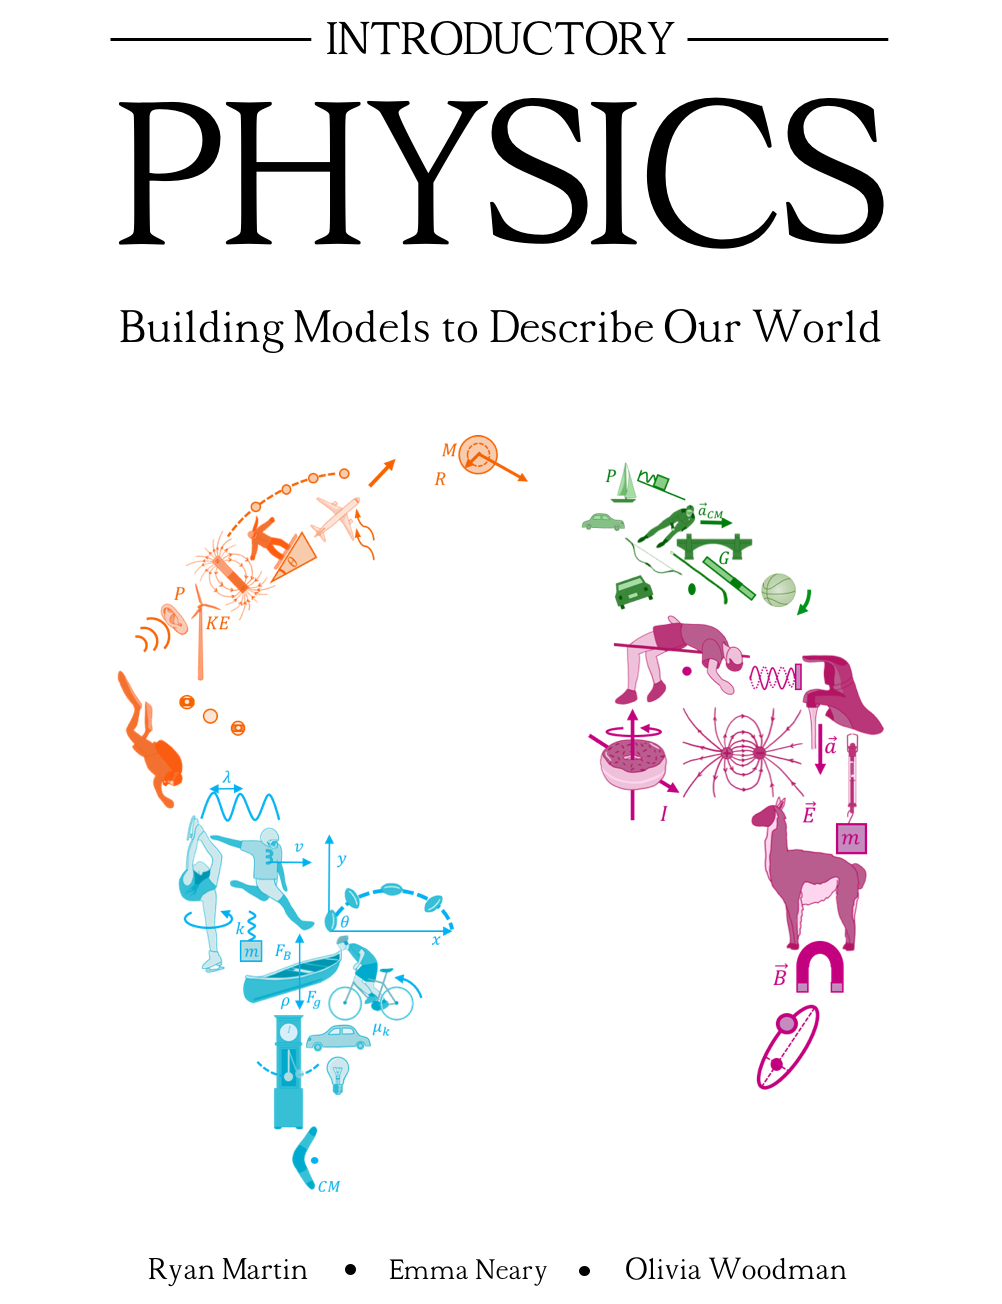
\includegraphics[width=\textwidth]{figures/CoverPage/coverpage.png}
\null
\vfill

\pagenumbering{roman}
\section*{License}
This textbook is shared under the CC-BY-SA 3.0 (Creative Commons) license. You are free to copy and redistribute the material in any medium or format, remix, transform, and build upon the material for any purpose, even commercially. You must give appropriate credit, provide a link to the license, and indicate if changes were made. You may do so in any reasonable manner, but not in any way that suggests the licensor endorses you or your use. If you remix, transform, or build upon the material, you must distribute your contributions under the same license as the original.
\vspace{\fill}
\begin{center}

\includegraphics[width=0.4\textwidth]{figures/Preface/license.png}
\end{center}
\newpage

\chapter*{Preface}
\label{chap:ipreface}
\section*{About this textbook}
This textbook is written to fill several needs that we believe were not already met by the many existing introductory physics textbooks. First, we wanted to ensure that the textbook is free to use for students and professors. Second, we wanted to design a textbook that is mindful of the new pedagogies being used in introductory physics, by writing it in a way that is adapted to a flipped-classroom approach where students complete readings, think about the readings, and then discuss the material in class. Third, we wanted to create a textbook that also addresses the experimental aspect of physics, by proposing experiments to be conducted at home or in the lab, as well as providing guidelines for designing experiments and reporting on experimental results. Finally, we wanted to create a textbook that is a sort of ``living document'', that professors can edit and re-mix for their own needs, and to which students can contribute material as well. The textbook is hosted on \href{https://github.com/OSTP/PhysicsArtofModelling}{GitHub}, which allows anyone to make suggestions, point out issues and mistakes, and contribute material.

This textbook is meant to be paired with the accompanying ``Question Library'', which contains many practice problems, many of which were contributed by students.

This textbook would not have been possible without the support of Queen's University and the Department of Physics, Engineering Physics \& Astronomy at Queen's University, as well as the many helpful discussions with the students, technicians and professors at Queen's University.

\section*{Hello from the authors}
\lwfig[9]{0.2\textwidth}{figures/Preface/Ryan.png}
\textbf{Ryan Martin} I am a professor of physics at Queen's University. My main research is in the field of particle astrophysics, particularly in studying the properties of neutrinos. I grew up in Switzerland, obtained my Bachelor's, Master's and Ph.D. at Queen's University. I was then a postdoctoral fellow at Lawrence Berkeley National Laboratory, a faculty at the University of South Dakota, before returning to Queen's. I am particularly passionate about education, and I am always seeking opportunities to involve students in helping to make education more accessible. I also like to cook and to play volleyball.

\lwfig[9]{0.2\textwidth}{figures/Preface/Emma.jpg}
\textbf{Emma Neary} I am currently a second year physics major and QuARMS (Queen's University Accelerated Route to Medical School) student, as well as a native of St. John's, Newfoundland. Uniting the perspectives of students and professors in an accessible way is important to me. I strongly believe in the importance of building physical models; whether it be in physics, medicine, sciences or the arts. It has been my goal to infuse the textbook with the theme of modelling in a creative and engaging way. Aside from doing physics, I enjoy hiking, dancing, reading and doing research in gastroenterology and neuropsychiatry.

\lwfig[9]{0.2\textwidth}{figures/Preface/josh.png}
\textbf{Joshua Rinaldo} I am a third year physics major and concurrent education student. I was first introduced to the flipped classroom approach in Ryan Martin's first year physics class, and have found that the experience shaped the way I approach education. I intend on continuing to make use of the flipped classroom approach as I move forward in my career. Being able to co-author this textbook has been an amazing opportunity for me to grow as an educator, and I look forward to applying the skills I learned while working on the textbook. Outside of physics, I enjoy making jewelry and practicing mixed martial arts.

\lwfig[9]{0.2\textwidth}{figures/Preface/Olivia.png}
\textbf{Olivia Woodman} I am a currently a third year undergraduate student at Queen's Univeristy, majoring in physics. The flipped classroom approach has been beneficial to my own learning, and I think that we have created a textbook that really complements this learning style. Throughout this book, I have shared my thoughts on various topics in physics, as well as some useful tips and tricks. I hope that students enjoy using this book and continue to contribute to it in the future. Working on this textbook has also allowed me to combine my love of physics with my love of doodling, so I hope you enjoy the drawings!

\section*{How to use this textbook}
This textbook is designed to be used in a flipped-classroom approach, where students complete readings at home, and the material is then discussed in class. The material is thus presented fairly succinctly, and contains \textbf{Checkpoint Questions} throughout that are meant to be answered as the students complete the reading. We suggest including these Checkpoint Questions as part of a quiz in a reading assignment (marked based on completion, not correctness), and then using these questions as a starting point for discussions in class.

For topics that are particularly difficult, we have included \textbf{Thought Boxes} written by students that try to present the material in a different light. We are always happy if students (or professors) wish to contribute additional thought boxes.

Chapters start with a set of \textbf{Learning outcomes} and an \textbf{Opening question} to help students have a sense of the chapter contents. The chapters have \textbf{Examples} throughout, as well as additional practice problems at the end. The \textbf{Question Library} should be consulted for additional practice problems. At the end of the chapter, a \textbf{Summary} presents the key points from the chapter. We suggest that students carefully read the summaries to make sure that they understand the contents of the chapter (and potentially identify, before reading the chapter, if the content is review to them). At the end of the chapters, we also present a section to \textbf{Think about the material}. This includes questions that can be assigned in reading assignments to research applications of the material or historical context. The thinking about the material section also includes experiments that can be done at home (as part of the reading assignment) or in the lab.

Appendices cover the main background in mathematics (Calculus and Vectors), as well as present an introduction to programming in python, which we feel is a useful skill to have in science. There is also an Appendix that is intended to guide work in the lab, by providing examples of how to write experimental proposals and reports, as well as guidelines for reviewing proposals and reports. We believe that introductory laboratories should not be be ``recipe-based'', but rather that students should take an approach similar to that of a researcher in designing (proposing) an experiment, conducting it, and reviewing the proposals and results of their peers.

\section*{Credits}
This textbook, and especially the many questions in the Question Library would not have been possible without the many contributions from students, teaching assistants and other professors. Below is a list of the students that have contributed material that have made this textbook and the Question Library possible.

\begin{multicols}{3}
\begin{center}
Adam McCaw\\
Ali Pirhadi\\
Alex Hughes\\
Alexis Brossard\\
Allyson Smith\\
Amy Van Nest\\
Camren Oakes\\
Ceaira Hiemstra\\
Damara Gagnier\\
Daniel Barake \\
Daniel Tazbaz\\
David Cutler\\
Emily Darling\\
Emily Mendelson\\
Emily Wener\\
Emma Lanciault\\
Erin Parson\\
Genevieve Fawcett\\
Gregory Love\\
Haoyuan Wang\\
Ian McClean\\
Jack Fitzgerald\\
James Godfrey\\
\columnbreak
Jenna Vanker\\
Jesse Fu\\
Jesse Simmons\\
Jessica Grennan\\
Joanna Fu\\
Jonathan Abott\\
Kate Fenwick\\
Lily Dodd\\
Madison Facchini\\
Marie Vidal\\
Matt Routliffe\\
Maya Gibb\\
Natalie Dubas\\
Nathan Wilson\\
Neil Rajan\\
Nicholas Everton\\
Nick Brown\\
Nicole Gaul\\
Noah Rowe\\
Olivia Bouaban\\
Patrick Singal\\
Qiqi Zhang\\
Quentin Sanders\\
\columnbreak
Robin Joshi\\
Ryan Underwood\\
Sam Connolly\\
Sara Stephens\\
Sarmund Mahmood\\
Shaundra Buelow\\
Shona Birkett\\
Stephanie Ciccone\\
Tai Withers\\
Talia Castillo\\
Tamy Puniani\\
Thomas Faour\\
Troy Allen\\
Tashifa Imtiaz\\
Wei Zhuolin\\
Yannick Bisson\\
Yumian Chen\\
Zifeng Chen\\
Zoe Macmillan
\end{center}
\end{multicols}

\tableofcontents
\pagenumbering{arabic}


%
\chapter{The Scientific Method and Physics}
\label{chap:introduction}

\begin{learningObjectives}
{\item Understand the Scientific Method.
\item Define the scope of Physics.
\item Understand the difference between theory and model.
\item Have a sense of how a physicist thinks.}
\end{learningObjectives}
\begin{opening}
\begin{MCquestion}{A scientific theory...}
\item must explain the physical world, and it may or may not be experimentally verifiable.
\item proves our models to be correct, and it must be experimentally verifiable.
\item describes the physical world, and must be experimentally verifiable. \correct
\item must disprove other theories, and may or may not be experimentally verifiable.
\end{MCquestion}
\end{opening}
\vspace{0.5cm}
\section{Science and the Scientific Method}
Science is the process of \textit{describing} the world around us. It is important to note that describing the world around us is not the same as \textit{explaining} the world around us. Science aims to answer the question ``How?'' and not the question ``Why?''. As we develop our description of the physical world, you should remember this important distinction and resist the urge to ask ``Why?''.

The Scientific Method is a prescription for coming up with a description of the physical world that anyone can challenge and improve through performing experiments. If we come up with a description that can describe many observations, or the outcome of many different experiments, then we usually call that description a ``Scientific Theory''. We can get some insight into the Scientific Method through a simple example. 

Imagine that we wish to describe how long it takes for a tennis ball to reach the ground after being released from a certain height. One way to proceed is to describe how long it takes for a tennis ball to drop \SI{1}{\meter}, and then to describe how long it takes for a tennis ball to drop \SI{2}{\meter}, etc. We could generate a giant table showing how long it takes a tennis ball to drop from any given height. Someone would then be able to perform an experiment to measure how long a tennis ball takes to drop from \SI{1}{\meter} or \SI{2}{\meter} and see if their measurement disagrees with the tabulated values. If we collected the descriptions for all possible heights, then we would effectively have a valid and testable scientific theory that describes how long it takes tennis balls to drop from any height.

Suppose that a budding scientist, let's call her Chlo\"e, then came along and noticed that there is a pattern in the theory that can be described much more succinctly and generally than by using a giant table. In particular, suppose that she notices that, mathematically, the time, $t$, that it takes for a tennis ball to drop a height, $h$, is proportional to the square root of the height:
\begin{equation*}
t \propto \sqrt{h}
\end{equation*}

\begin{example}{Use Chlo\"e's Theory ($t \propto \sqrt{h}$) to determine how much longer it will take for an object to drop by \SI{2}{\meter} than it would to drop by \SI{1}{\meter}.}

When we have a proportionality law (with a $\propto$) sign, we can always change this to an equal sign by introducing a constant, which we will call $k$:
\begin{align*}
t &\propto \sqrt{h} \\
\rightarrow t&=k\sqrt{h}
\end{align*}
Let $t_1$ be the time to fall a distance $h_1=\SI{1}{\meter}$, and $t_2$ be the time to fall a distance $h_2=\SI{2}{\meter}$. In terms of our unknown constant, $k$, we have:
\begin{align*}
t_1 &=k\sqrt{h_1}=k \sqrt{(\SI{1}{\meter})}\\
t_2 &=k\sqrt{h_2}=k \sqrt{(\SI{2}{\meter})}\\
\end{align*}
By taking the ratio, $\frac{t_1}{t_2}$, our unknown constant $k$ will cancel:
\begin{align*}
\frac{t_1}{t_2}&=\frac{\sqrt{(\SI{1}{\meter})}}{\sqrt{(\SI{2}{\meter})}}=\frac{1}{\sqrt 2}\\
\therefore t_2 &= \sqrt{2} t_1
\end{align*}
and we find that it will take $\sqrt{2}\sim 1.41$ times longer to drop by \SI{2}{\meter} than it will by \SI{1}{\meter}.
\end{example}

Chlo\"e's ``Theory of Tennis Ball Drop Times'' is appealing because it is succinct, and it also allows us to make \textbf{verifiable predictions}. That is, using this theory, we can predict that it will take a tennis ball $\sqrt 2$ times longer to drop from \SI{2}{\meter} than it will from \SI{1}{\meter}, and then perform an experiment to verify that prediction. If the experiment agrees with the prediction, then we conclude that Chlo\"e's theory adequately describes the result of that particular experiment. If the experiment does not agree with the prediction, then we conclude that the theory is not an adequate description of that experiment, and we try to find a new theory.

Chlo\"e's theory is also appealing because it can describe not only tennis balls, but the time it takes for other objects to fall as well. Scientists can then set out to continue testing her theory with a wide range of objects and drop heights to see if it describes those experiments as well. Inevitably, they will discover situations where Chlo\"e's theory fails to adequately describe the time that it takes for objects to fall (can you think of an example?).

We would then develop a new ``Theory of Falling Objects'' that would include Chlo\"e's theory that describes most objects falling, and additionally, a set of descriptions for the fall times for cases that are not described by Chlo\"e's theory. Ideally, we would seek a new theory that would also describe the new phenomena not described by Chlo\"e's theory in a succinct manner. There is of course no guarantee, ever, that such a theory would exist; it is just an optimistic hope of physicists to find the most general and succinct description of the physical world. This is a general difference between physics and many of the other sciences. In physics, one always tries to arrive at a succinct theory (e.g. an equation) that can describe many phenomena, whereas the other sciences are often very descriptive. For example, there is no succinct formula for how butterflies look; rather, there is a giant collection of observations of different butterflies.

This example highlights that applying the Scientific Method is an iterative process. Loosely, the prescription for applying the Scientific Method is:
\begin{enumerate}
\item Identify and describe a process that is not currently described by a theory.
\item Look at similar processes to see if they can be described in a similar way.
\item Improve the description to arrive at a ``Theory'' that can be generalized to make predictions.
\item Test predictions of the theory on new processes until a prediction fails.
\item Improve the theory.
\end{enumerate}

\begin{checkpoint}
\begin{MCquestion}{Fill in the blanks:

Physics is a branch of science that \underline{\hspace{2cm}} the behaviour of the universe. When doing physics, we attempt to answer the question of \underline{\hspace{2cm}} things work the way they do.}
\item explains
\item describes 
\item how 
\item why
\end{MCquestion}
\begin{answer}
\begin{enumerate}
\item describes
\item how
\end{enumerate}
\end{answer}
\end{checkpoint}

\section{Theories and models}
For the purpose of this textbook, we wish to introduce a distinction in what we mean by ``theory'' and by ``model''. We will consider a ``theory'' to be a set of statements that gives us a broad description, applicable to several phenomena and that allow us to make verifiable predictions. We will consider a ``model'' to be a situation-specific description of a phenomenon \textit{based on a theory}, that allows to make a specific prediction. Using the example from the previous section, our theory would be that the fall time of an object is proportional to the square root of the drop height, and a model would be applying that theory to describe a tennis ball falling by \SI{4.2}{\meter}.

This textbook will introduce the theories from Classical Physics, which were mostly established and tested between the seventeenth and nineteenth centuries. We will take it as given that readers of this textbook are not likely to perform experiments that challenge those well-established theories. The main challenge will be, given a theory, to define a model that describes a particular situation, and then to test that model. This introductory physics course is thus focused on thinking of ``doing physics'' as the task of correctly modelling a situation.
\newpage
\begin{studentOpinion}{Emma}{\textbf{What's the difference between a model and a theory?}}\\
``Model'' and ``Theory'' are sometimes used interchangeably among scientists. In physics, it is particularly important to distinguish between these two terms. A model provides an immediate understanding of something based on a theory. 

For example, if you would like to model the launch of your toy rocket into space, you might run a computer simulation of the launch based on various theories of propulsion that you have learned. In this case, the model is the computer simulation, which describes what will happen to the rocket. This model depends on various theories that have been extensively tested such as Newton's Laws of motion, Fluid dynamics, etc. 
\begin{itemize}
\item``Model'': Your homemade rocket computer simulation
\item``Theory'': Newton's Laws of motion, Fluid dynamics
\end{itemize}
With this analogy, we can quickly see that the ``model'' and ``theory'' are not interchangeable. If they were, we would be saying that all of Newton's Laws of Motion depend on the success of your piddly toy rocket computer simulation!
\end{studentOpinion}

\begin{checkpoint}
\begin{MCquestion}{Models cannot be scientifically tested, only theories can be tested.}
\item True
\item False \correct
\end{MCquestion}
\end{checkpoint}

\section{Fighting intuition}
It is important to remember to fight one's intuition when applying the scientific method. Certain theories, such as Quantum Mechanics, are very counter-intuitive. For example, in Quantum Mechanics, an object can be described as being in two locations at the same time. In the Theory of Special Relativity, it is possible for two people to disagree on whether two events occurred at the same time. These particular prediction from these theories have not been invalidated by any experiment.

There is no requirement in science that a theory be ``pretty'' or intuitive. The only requirement is that a theory describe experimental data. One should then take care in not forcing one's preconceived notions into interpreting a theory. For example, Quantum Mechanics does not actually predict that objects can be in two locations at once, only that objects behave \textit{as if} they were in two locations at once. A famous example is Schr\"odinger's cat, which can be modelled as being both alive and dead at the same time. However, just because we model it that way does not mean that it really is alive and dead at the same time. 

\section{The scope of Physics}
Physics describes a wide range of phenomena within the physical sciences, ranging from the behaviour of microscopic particles that make up matter to the evolution of the entire Universe. We often distinguish between ``classical'' and ``modern'' physics depending on when the theories were developed, and we can further subdivide these areas of physics depending on the scale or the type of the phenomena that they describe.

The word physics comes from Ancient Greek and translates to ``nature'' or ``knowledge of nature''. The goal of physics is to develop theories from which mathematical models can be derived to describe our observations. One of the ambitious goals of physicists is to develop a single theory that describes all of nature, instead of having multiple theories to describe different categories of phenomena. This is in stark contrast to other fields of science, as Rutherford famously quipped: ``All science is either physics or stamp collecting''. That is, physicists hope that there exists one single mathematical theory (like Chlo\"e's theory of falling objects) that describes the entire physical world. In Biology, for example, this would not be a reasonable goal, as one needs to describe every single living being, and there is no overarching ``theory of what all living things look like''. Currently, physicists have been able to narrow down the number of theories required to describe all of the physical world to only three, which is impressive (the theory of gravity, the theory of the strong nuclear force, and physicists have now further unified the weak nuclear force with electromagnetism to make the ``electroweak force'').


\subsection{Classical Physics}
This textbook is focused on classical physics, which corresponds to the theories that were developed before 1905.
\subsubsection{Mechanics}
Mechanics describes most of our everyday experiences, such as how objects move, including how planets move under the influence of gravity. Isaac Newton was the first to formally develop a theory of mechanics, using his ``Three Laws'' to describe the behaviour of objects in our everyday experience. His famous work published in 1687, ``Philosophiae Naturalis Principia Mathematica'' (``The Principia'') also included a theory of gravity that describes the motion of celestial objects. 

Following the 1781 discovery of the planet Uranus by William Herschel, astronomers noticed that the orbit of the planet was not well described by Newton's theory. This led Urbain Le Verrier (in Paris) and John Couch Adams (in Cambridge) to predict the location of a new planet that was disturbing the orbit of Uranus rather than to claim that Newton's theory was incorrect. The planet Neptune was subsequently discovered by Le Verrier in 1846, one year after the prediction, and seen as a resounding confirmation of Newton's theory. 

In 1859, Urbain Le Verrier also noted that Mercury's orbit around the Sun is different than that predicted by Newton's theory. Again, a new planet was proposed, ``Vulcan'', but that planet was never discovered and the deviation of Mercury's orbit from Newton's prediction remained unexplained until 1915, when Albert Einstein introduced a new, more complete, theory of gravity, called ``General Relativity''. This is a good example of the scientific method; although the discovery of Neptune was consistent with Newton's theory, it did not prove that the theory is correct, only that it correctly described the motion of Uranus. The discrepancy that arose when looking at Mercury ultimately showed that Newtons' theory of gravity fails to provide a proper description of planetary orbits in the proximity of very massive objects (Mercury is the closest planet to the Sun). 

\begin{checkpoint}
\begin{MCquestion}{What did the inability to find the planet Vulcan show:}
\item It showed that Newton's model of Mercury was correct. 
\item It showed that Newton's theory did not correctly describe the orbits of all planets.\correct
\item It showed that the technology at the time was inadequate. 
\item It showed that Einstein's theory of General Relativity was correct. 
\end{MCquestion}
\end{checkpoint}
 

\subsubsection{Electromagnetism}
Electromagnetism describes electric charges and magnetism. At first, it was not realized that electricity and magnetism were connected. Charles Augustin de Coulomb published in 1784 the first description of how electric charges attract and repel each other. Magnetism was discovered in the ancient world, when people noticed that lodestone (rocks made from magnetized magnetite mineral) could attract iron tools. In 1819, Oersted discovered that moving electric charges could influence a compass needle, and several subsequent experiments were carried out to discover how magnets and moving electric charges interact.

In 1865, James Clerk Maxwell published ``A Dynamical Theory of the Electromagnetic Field'', wherein he first proposed a theory that unified electricity and magnetism as two facets of the same phenomenon. One important concept from Maxwell's theory is that light is an electromagnetic wave with a well-defined speed. This uncovered some potential issues with the theory as it required an absolute frame of reference in which to describe the propagation of light. Experiments in the late 1800s failed to detect the existence of this frame of reference.

\subsection{Modern Physics}
In 1905, Albert Einstein published three major papers that set the foundation for what we now call ``Modern Physics''. These papers covered the following areas that were not well-described by classical physics:
\begin{itemize}
\item A description of Brownian motion that implied that all matter is made of atoms.
\item A description of the photoelectric effect that implied that light is made of particles.
\item A description of the motion of very fast objects that implied that mass is equivalent to energy, and that time and distance are relative concepts.
\end{itemize}
In order to accommodate Einstein's descriptions, physicists had to dramatically re-formulate new theories. 

\subsubsection{Quantum mechanics and particle physics}
Quantum mechanics is a theory that was developed in the 1920s to incorporate Einstein's conclusion that light is made of particles (or rather, quantized lumps of energy called quanta) and describe nature at the smallest scales. This could only be done at the expense of determinism, the idea that we can predict how particular situations evolve in time. This led to a theory that could only provide the \textit{probabilities} that certain outcomes will be realized. Quantum mechanics was further refined during the twentieth century into Quantum Field Theory, which led to the Standard Model of particle physics that describes our current understanding of matter through the theories of the electroweak and strong forces.

\subsubsection{The Special and General Theories of Relativity}
In 1905, Einstein published his ``Special Theory of Relativity'', which describes how light propagates at a constant speed without the need for an absolute frame of reference, thus solving the problem introduced by Maxwell. This required physicists to consider space and time on an equal footing (``space-time''), rather than two independent aspects of the natural world, and led to a flurry of odd, but verified, experimental predictions. One such prediction is that time flows slower for objects that are moving fast, which has been experimentally verified by flying precise atomic clocks on airplanes and satellites. In 1915, Einstein further refined his theory into General Relativity, which is our best current description of gravity and includes a description of Mercury's orbit which was not described by Newton's theory.

\begin{checkpoint}
\begin{MCquestion}{Special relativity can be applied to which of these science fiction plots?}
\item An eccentric duo travel back in time to alter the past. 
\item An astronaut travelling near light speed for many years comes home to find that he has aged less than his family on Earth. \correct
\item A superhero harnesses lightning to use as a weapon.
\end{MCquestion}
\end{checkpoint}

\subsubsection{Cosmology and astrophysics} 
Cosmology describes processes at the largest scales and is mostly based on applying General Relativity to the scale of the Universe. For example, cosmology describes how our Universe started from the Big Bang and how large scale structures, such as galaxies and clusters of galaxies, have formed and evolved into our present day Universe. 

\capfig{0.3\textwidth}{figures/Introduction/galaxies_in_Coma_cluster.jpeg}{\label{fig:introduction:galaxiescomacluster}A galaxy in the Coma cluster of galaxies (credit:NASA).}

Astrophysics is focused on describing the formation and the evolution of stars, galaxies, and other ``astrophysical objects'' such as neutron stars and black holes. 

\subsubsection{Particle astrophysics}
Particle astrophysics is a relatively new field that makes use of subatomic particles produced by astrophysical objects to learn both about the objects \textit{and} about the particles. For example, the 2015 Nobel Prize in Physics was awarded to Art McDonald (a Canadian physicist from Queen's University) for using neutrinos\footnote{Neutrinos are the lightest subatomic particles that we know of} produced by the Sun to both learn about the nature of neutrinos and about how the Sun works. 

\section{Thinking like a physicist}
In a sense, physics can be thought of as the most fundamental of the sciences, as it describes the interactions of the smallest constituents of matter. In principle, if one can precisely describe how protons, neutrons, and electrons interact, then one can completely describe how a human brain thinks. In practice, the theories of particle physics lead to equations that are too difficult to solve for systems that include as many particles as a human brain. In fact, they are too difficult to solve exactly for even rather small systems of particles such as atoms bigger than helium (containing several protons, neutrons and electrons). 

We have a number of other fields of science to cover complex systems of particles interacting. Chemistry can be used to describe what happens to systems consisting of many atoms and molecules. In a living being, it is too difficult to keep track of systems of atoms and molecules, so we use Biology to describe living systems. 

One of the key qualities required to be an effective physicist is an ability to understand how to apply a theory and develop a model to describe a phenomenon. Just like any other skill, it takes practice to become good at developing models. Students that graduate with a physics degree are thus often sought for jobs that require critical thinking and the ability to develop quantitative models, which covers many fields from outside of physics such as finance or Big Data. This textbook thus tries to emphasize practice with developing models, while also providing a strong background in the theories of classical physics. 

\newpage
\section{Summary}
\vspace{0.5cm}
\begin{chapterSummary}
Science attempts to \textit{describe} the physical world (it answers the question ``How?'', not ``Why?''). 

The Scientific Method provides a prescription for arriving at theories that describe the physical world and can be experimentally verified. The Scientific Method is necessarily an iterative process where theories are continuously updated as new experimental data are acquired. An experiment can only disprove a theory, not confirm it in any general sense.

Physics covers a wide scale of phenomena ranging from the Universe down to subatomic particles. Classical physics encompasses the theories developed before 1905, when Einstein introduced the need for Quantum Mechanics and the Theorie(s) of Relativity. One of the main goals of physics is to arrive at a single theory that describes all of our natural world. Currently, physicists require three theories to describe the natural world.

\end{chapterSummary}

\section{Thinking about the Material}
\vspace{0.5cm}
\begin{chapteractivity}{Reflect and research}
{
\item What particle helps to give mass to all of the massive elementary particles?
\item Name that physicist! Who was the first to propose that the universe is expanding?
\item Before discovering the CMBR (Cosmic Microwave Background Radiation), scientists Arno Penzias and Robert Wilson were trying to detect radio waves with very sensitive antennae. The very first time they heard a consistent, low noise on their detectors they discovered that it was (mostly) not the CMBR. What was causing most of this noise?
\item Physicist Lene Hau first slowed a beam of light to $\SI{17}{m/s}$ using a very cold, dilute gas of bosons. In 2001, how fast was she able to slow down the beam of light?
\item Think of two theories that you use in your every day life. (For example, when we wash our hands, we do so because of the germ theory of disease!)
}
\end{chapteractivity}

\newpage
\section{Sample problems and solutions}
\subsection{Problems}
\begin{problemParts}{soln:introduction:chemtrails}{\label{prob:introduction:chemtrails} Your friend Martin loves to explore ``conspiracy theories''. His favourite theory involves ``Chem Trails''. He tells you that the government is secretly using airliners to spread chemicals in the atmosphere for some unknown reason.}
\item Think of 2 ways in which you could objectively test Martin's theory.
\item After proposing your experiment to Martin, he claims that his theory cannot be invalidated by any experiment, no matter how scientifically rigorous the experiment is. Is Martin correct?
\end{problemParts}
\newpage
\subsection{Solutions}
\begin{solution}{prob:introduction:chemtrails}\label{soln:introduction:chemtrails}


a) You could do an investigation to see if the government is spreading chemicals, and try to find out why. You could make measurements of the contents in the atmosphere before and after an airline passes to see if any unexpected chemicals show up.

b) No he is not, as you just proposed two experiments that could invalidate his theory.
\end{solution}






%
\chapter{Comparing Model and Experiment}
\label{chap:modelandexperiment}
In this chapter, we will learn about the process of doing science and lay the foundations for developing skills that will be of use throughout your scientific careers. In particular, we will start to learn how to test a model with an experiment, as well as learn to estimate whether a given result or model makes sense.
\begin{learningObjectives}{
\item Be able to estimate orders of magnitude.
\item Understand units.
\item Understand the process of building a model and performing an experiment.
\item Understand uncertainties in experiments.}
\end{learningObjectives}
\begin{opening}
\begin{MCquestion}{Newton's Universal Theory of Gravity predicts that objects near the surface of the Earth will fall with an acceleration of $\SI{9.8}{m/s^2}$. Your friend reports that they have measured the acceleration of a falling ball and found that it was $\SI{9.0\pm 0.5}{m/s^2}$. Does their result invalidate the prediction from Newton's Theory?}
\item Yes, since the range $\SI{9.0\pm 0.5}{m/s^2}$ does not include $\SI{9.8}{m/s^2}$.
\item Not necessarily, as it depends on whether your friend correctly determined the uncertainty in their measurement.\correct
\item Definitely not, since Newton's Universal Theory of Gravity has been confirmed by many experiments.
\end{MCquestion}
\end{opening}

\section{Orders of magnitude}
Although you should try to fight intuition when building a model to describe a particular phenomenon, you should not abandon critical thinking and should always ask if a prediction from your model makes sense. One of the most straightforward ways to estimate if a model makes sense is to ask whether it predicts the correct order of magnitude for a quantity. Usually, the order of magnitude for a quantity can be determined by making a very simple model, ideally one that you can work through in your head. When we say that a prediction gives the right ``order of magnitude'', we usually mean that the prediction is within a factor of ``a few'' (up to a factor of 10) of the correct answer. For example, if a measurement gives a value of 2000, then we would consider that a model prediction of 8000 gave the right order of magnitude (it differs from the correct answer by a factor of 4), whereas a prediction of 24000 would not (it differs by a factor of 12). 

\begin{example}{How many ping pong balls can you fit into a school bus? Is it of order 10,000, or 100,000, or more?}
Our strategy is to estimate the volumes of a school bus and of a ping pong ball, and then calculate how many times the volume of the ping pong ball fits into the volume of the school bus.

We can model a school bus as a box, say $\SI{20}{\meter}\times \SI{2}{\meter}\times\SI{2}{\meter}$, with a volume of \SI{80}{\meter\cubed}$\sim$\SI{100}{\meter\cubed}. We can model a ping pong ball as a sphere with a diameter of \SI{0.03}{\meter} (\SI{3}{\centi\meter}). When stacking the ping pong balls, we can model them as little cubes with a side given by their diameter, so the volume of a ping pong ball, for stacking, is $\sim$ \SI{0.00003}{\meter\cubed}=\SI{3e-5}{\meter\cubed}. If we divide \SI{100}{\meter\cubed} by \SI{3e-5}{\meter\cubed}, using scientific notation:
\begin{align*}
\frac{\SI{100}{\meter\cubed}}{\SI{3e-5}{\meter\cubed}}=\frac{\num{1e2}}{\num{3e-5}}=\frac{1}{3}\times 10^7\sim 3\times 10^6
\end{align*}
Thus, we expect to be able to fit about three million ping pong balls in a school bus. 

\capfig{0.55\textwidth}{figures/ModelAndExperiment/schoolbusestimate.png}{\label{fig:modelandexperiment:schoolbusestimate}A school bus and ping pong balls modelled as boxes.}

\end{example}

\begin{checkpoint}{Fill in the following table, giving the order of magnitude (in meters) of the sizes of different physical objects. Feel free to look these up on the internet!}
\begin{center}
\begin{tabular}{|c|c|}
\hline  
\textbf{Object}&\textbf{Order of magnitude}\\
\hline
Proton&\\ \hline 
Nucleus of atom&\\ \hline
Hydrogen atom&\\ \hline
Virus&\\ \hline
Human skin cell&\\ \hline
Width of human hair&\\ \hline
Human &\SI{1}{\meter}\\ \hline
Height of Mt. Everest&\\ \hline
Radius of the Earth&\\ \hline
Radius of the Sun&\\ \hline
Radius of the Milky Way&\\ \hline
\end{tabular}
\end{center}
\begin{answer}
\begin{center}
\begin{tabular}{|c|c|}
\hline  
\textbf{Object}&\textbf{Order of magnitude}\\
\hline
Proton&\SI{1e-15}{m}\\ \hline 
Nucleus of atom&\SI{1e-14}{m}\\ \hline
Hydrogen atom&\SI{1e-10}{m}\\ \hline
Virus&\SI{1e-7}{m}\\ \hline
Human skin cell&\SI{1e-5}{m}\\ \hline
Width of human hair&\SI{1e-4}{m}\\ \hline
Human &\SI{1}{\meter}\\ \hline
Height of Mt. Everest&\SI{1e3}{m}\\ \hline
Radius of the Earth&\SI{1e7}{m}\\ \hline
Radius of the Sun&\SI{1e9}{m}\\ \hline
Radius of the Milky Way&\SI{1e21}{m}\\ \hline
\end{tabular}
\end{center}
\end{answer}
\end{checkpoint}


\section{Units and dimensions}
In 1999, the NASA Mars Climate Orbiter disintegrated in the Martian atmosphere because of a mixup in the units used to calculate the thrust needed to slow the probe and place it in orbit about Mars. A computer program provided by a private manufacturer used units of pounds seconds to calculate the change in momentum of the probe instead of the Newton seconds expected by NASA. As a result, the probe was slowed down too much and disintegrated in the Martian atmosphere. This example illustrates the need for us to \textbf{use and specify units} when we describe the properties of a physical quantity, and it also demonstrates the difference between a dimension and a unit.

``Dimensions'' can be thought of as types of measurements. For example, length and time are both dimensions. A unit is the standard that we choose to quantify a dimension. For example, meters and feet are both units for the dimension of length, whereas seconds and jiffys\footnote{A jiffy is a unit used in electronics and generally corresponds to either 1/50 or 1/60 seconds.} are units for the dimension of time.

When we compare two numbers, for example a prediction from a model and a measurement, it is important that both quantities have the same dimension \textit{and} be expressed in the same units.
\begin{checkpoint}
\begin{MCquestion}{The speed limit on a highway...}
\item has the dimension of length over time and can be expressed in units of kilometers per hour. \correct
\item has the dimension of length can and be expressed in units of kilometers per hour.
\item has the dimension of time over length and can be expressed in units of meters per second.
\item has the dimension of time and can be expressed in units of meters.
\end{MCquestion}
\end{checkpoint}

\subsection{Base dimensions and their SI units}
In order to facilitate communication of scientific information, the International System of units (SI for the french, Syst\`eme International d'unit\'es) was developed. This allows us to use a well-defined convention for which units to use when describing quantities. For example, the SI unit for the dimension of length is the meter and the SI unit for the dimension of time is the second.

In order to simplify the SI unit system, a fundamental (base) set of dimensions was chosen and the SI units were defined for those dimensions. Any other dimension can always be re-expressed in terms of the base dimensions shown in Table \ref{tab:modelandexperiment:SIunits} and its units in terms of the corresponding combination of the base SI units.

\begin{center}
\begin{tabular}{ll }
\textbf{Dimension}&\textbf{SI unit}\\
\hline
\hline
Length [L]& meter [m]\\ \hline
Time [T]& seconds[s] \\ \hline
Mass [M]& kilogram [kg]\\ \hline
Temperature [$\Theta$]& kelvin [K] \\ \hline
Electric current [I]& amp\`ere [A]\\ \hline
Amount of substance [N]& mole [mol] \\ \hline
Luminous intensity [J]& candela [cd] \\ \hline
Dimensionless [1]& unitless [] \\ \hline
\end{tabular}
\captionof{table}{\label{tab:modelandexperiment:SIunits} Base dimensions and their SI units with abbreviations.}
\end{center}

From the base dimensions, one can obtain ``derived'' dimensions such as ``speed'' which is a measure of how fast an object is moving. The dimension of speed is $L/T$ (length over time) and the corresponding SI unit is m/s (meters per second)\footnote{Note that we can also write meters per second as m$\cdot$s$^{-1}$, but we often use a divide by sign if the power of the unit in the denominator is 1.} Many of the derived dimension have corresponding derived SI units which can be expressed in terms of the base SI units. Table \ref{tab:modelandexperiment:derivedSIunits} shows a few derived dimensions and their corresponding SI units and how those SI units are obtained from the base SI units.

\begin{table}[!h]
\centering
\begin{tabular}{lll }  
\textbf{Dimension}&\textbf{SI unit}&\textbf{SI base units}\\
\hline
\hline
Speed [L/T]& meter per second [m/s] & [m/s]\\ \hline
Frequency [1/T]& hertz [Hz] & [1/s]\\ \hline
Force [M$\cdot$L$\cdot$T$^{-2}$]& newton [N]&[kg$\cdot$m$\cdot$s$^{-2}$]\\ \hline
Energy [M$\cdot$L$^2\cdot$T$^{-2}$]& joule [J]&[N$\cdot$m=kg$\cdot$m$^2\cdot$s$^{-2}$] \\ \hline
Power [M$\cdot$L$^2\cdot$T$^{-3}$]& watt [W]&[J/s=kg$\cdot$m$^2\cdot$s$^{-3}$]\\ \hline
Electric Charge [I$\cdot$ T]& coulomb [C]&[A$\cdot$ s] \\ \hline
Voltage [M$\cdot$L$^2\cdot$T$^{-3}\cdot$I$^{-1}$]& volt [V]&[J/C=kg$\cdot$m$^2\cdot$s$^{-3}\cdot$A$^{-1}$] \\ \hline
\end{tabular}
\caption{\label{tab:modelandexperiment:derivedSIunits} Example of derived dimensions and their SI units with abbreviations.}
\end{table}

By convention, we can indicate the dimension of a quantity, $X$, by writing it in square brackets, $[X]$. For example, $[X]=I$, would mean that the quantity $X$ has the dimension $I$, so it has the dimension of electric current. Similarly, we can indicate the SI units of $X$ with $SI[X]$. Referring to Table \ref{tab:modelandexperiment:SIunits}, since $X$ has the dimension of current, $SI[X]=A$.

\subsection{Dimensional analysis}
We call ``dimensional analysis'' the process of working out the dimensions of a quantity in terms of the base dimensions and a model prediction for that quantity. A few simple rules allow us to easily work out the dimensions of a derived quantity. Suppose that we have two quantities, $X$ and $Y$, both with dimensions. We then have the following rules to find the dimension of a quantity that depends on $X$ and $Y$:
\begin{enumerate}
\item Addition/Subtraction: You can only add or subtract two quantities if they have the same dimension: $[X+Y]=[X]=[Y]$
\item Multiplication: The dimension of the product, $[XY]$ , is the product of the dimensions: $[XY]=[X]\cdot[Y]$
\item Division: The dimension of the ratio, $[X/Y]$, is the ratio of the dimensions: $[X/Y]=[X]/[Y]$
\end{enumerate}
The next two examples show how to apply dimensional analysis to obtain the unit or dimension of a derived quantity. 
\newpage
\begin{example}{
\label{ex:modelandexperiment:forceSI} Acceleration has SI units of $\si{ms^{-2}}$ and force has the dimension of mass multiplied by acceleration. What are the dimensions and SI units of force, expressed in terms of the base dimensions and units?}
We can start by expressing the dimension of acceleration, since we know from its SI units that it must have the dimension of length over time squared.
\begin{align*}
[acceleration] = \frac{L}{T^2}
\end{align*}
Since force has the dimension of mass times acceleration, we have:
\begin{align*}
[force] = [mass]\cdot[acceleration] = M \frac{L}{T^2}
\end{align*}
and the SI units of force are thus:
\begin{align*}
SI[force] = \si{kg}\cdot\si{m/s^2}
\end{align*}
Force is such a common dimension that it, like many other derived dimensions, has its own derived SI unit, the Newton [N].
\end{example}

\begin{example}{Use Table \ref{tab:modelandexperiment:derivedSIunits} to show that voltage has the same dimension as force multiplied by speed and divided by electric current.}
According to Table \ref{tab:modelandexperiment:derivedSIunits}, voltage has the dimension:
\begin{align*}
[voltage]=M\cdot L^2 \cdot T^{-3}\cdot I^{-1}
\end{align*}
while force, speed and current have dimensions:
\begin{align*}
[force]&=M\cdot L\cdot T^{-2} \\
[speed]&=L\cdot T^{-1}\\
[current]&=I
\end{align*}
The dimension of force multiplied by speed divided by electric charge
\begin{align*}
\left[\frac{force\cdot speed}{current}\right]&=\frac{[force]\cdot [speed]}{[current]}=\frac{M\cdot L\cdot T^{-2} \cdot L\cdot T^{-1} }{I}\\
&=M\cdot L^2 \cdot T^{-3}\cdot I^{-1}
\end{align*}
where, in the last line, we combined the powers of the same dimensions. By inspection, this is the same dimension as voltage.
\end{example}

When you build a model to predict the value of a physical quantity, you should always use dimensional analysis to ensure that the dimension of the quantity your model predicts is correct.

\begin{example}{Your model predicts that the speed, $v$, of an object of mass $m$, after having fallen a distance $h$ on the surface of a planet with mass $M$ and radius $R$ is given by:
\begin{align*}
v = \frac{mMh}{R}
\end{align*}
Is this a reasonable prediction?
}

First, we can see that the speed will be larger if $h$ is bigger, which makes sense, since we expect the speed to be greater if the object fell a greater distance. Similarly, we expect that the speed would be higher if the mass of the planet, $M$, is larger, as it would exert a larger gravitational force, as given by this model. We also expect that the object will have a greater speed if it has a larger mass, $m$, if the drag from the atmosphere on the planet is significant. Finally, if the radius of the planet $R$ is larger, we would expect the speed to be smaller, as the planet would be less dense and exert less gravitational force at its surface. However, if we verify the dimensions for the prediction of $v$, we find the model does not predict dimensions of speed:
\begin{align*}
[v] &= \frac{[m][M][h]}{[R]}\\
&=\frac{MML}{L}=M^2
\end{align*} 
and our model predicts a speed with dimensions of mass squared. By performing simple dimensional analysis, we can easily confirm that our model is definitely wrong. You should always check the dimensions of any model prediction, to make sure it is correct.
\end{example}

\begin{studentOpinion}{Olivia}
In this section, we were given three rules for combining dimensions. You'll notice that these rules are the same as the rules for algebra, except you're using dimensions instead of $x$'s and $y$'s. So, you can really just approach dimensional analysis problems as you would algebra problems.

There are some basic steps you can follow when you are trying to find the SI units for a value/variable in your equation. I'll go through Example \ref{ex:modelandexperiment:forceSI} in a bit of a different way. Let's say that you have the equation $F=ma$ and this time, you know the dimensions of $F$ and $m$, and you want to find the dimensions of $a$:
\begin{enumerate}[itemsep=1ex]
\item Rewrite the values/variables in your equation in terms of their dimensions, leaving all other operations (multiplication, exponents, etc.) as is: $F=m\cdot a\rightarrow [F]=[m]\cdot[a]$
\item Rearrange for your unknown dimension: $[a]=\frac{[F]}{[m]}$
\item Substitute in your known dimensions: $[a]=\frac{[F]}{[m]} \rightarrow [a]=\frac{MLT^{-2}}{M}=\frac{ML}{MT^2}$
\item Solve using the rules of algebra: $[a]=\frac{L}{T^2}$ (where we just cancelled out the $M$'s)
\item Replace the dimensions with their corresponding SI units: $[a]=\frac{L}{T^2}\rightarrow SI[a]=\frac{m}{s^2}$
\end{enumerate}
\end{studentOpinion}

\begin{checkpoint}
\begin{MCquestion}{In Chlo\"e's theory of falling objects from Chapter \ref{chap:introduction}, the time, $t$, for an object to fall a distance, $x$, was given by $t=k\sqrt{x}$. What must the SI units of Chlo\"e's constant, $k$, be?}
\item \si{T.L^{\frac{1}{2}}}
\item \si{T.L^{-\frac{1}{2}}}
\item \si{s.m^{\frac{1}{2}}}
\item \si{s.m^{-\frac{1}{2}}} \correct
\end{MCquestion}
\end{checkpoint}

Dimensional analysis can also be used to determine formulas (usually to within an order of magnitude). One famous example of this is when a British physicist named G.I. Taylor was able to determine a formula that showed how the blast radius of an atomic bomb scaled with time. Using pictures of the first atomic bomb explosion, he was able to determine the amount of energy released in the explosion, which was classified information at the time. 
\newpage
\begin{example}{Find a formula that shows how the blast radius, $r$, scales with the time since the explosion, $t$, where the radius also depends on the energy released in the explosion, $E$, and the density of the medium into which the bomb explodes, $\rho$.} 
We want to find out how the blast radius scales with time, so we want an expression that relates $r$ to some combination of $E$, $\rho$, and $t$:
\begin{align*}
r \sim E^x\rho^y t^z
\end{align*} 
where $x$, $y$, and $z$ are our unknown exponents, since we don't know yet how we will combine $E$, $\rho$, and $t$. However, we do know that when we combine these quantities, we have to get the correct dimension (length) for the radius:
\begin{align*}
[r]=[E]^x[\rho]^y[t]^z
\end{align*}
We know the dimensions for radius and time, and the dimension for $E$ can be found in Table \ref{tab:modelandexperiment:derivedSIunits}. Density is mass divided by volume, so its dimension is $M/L^3$. Our equation then becomes:
\begin{align*}
L&=(ML^2T^{-2})^x(ML^{-3})^y(T)^z\\
L&=(M^xL^{2x}T^{-2x})(M^yL^{-3y})(T^z)\\
\end{align*}
We have three unknowns, so we need three equations. We can recognize that the left hand side (with dimension of length, $L$) is equivalent to $L^1\cdot M^0\cdot T^0$. We can then separate the above expression into three equations, one for each of $M$, $L$, and $T$: 
\begin{align*}
M^0&=M^xM^y \rightarrow 0 = x+y\\
L^1&=L^{2x}L^{-3y} \rightarrow 1=2x-3y\\
T^0&=T^{-2x}T^{z} \rightarrow 0=z-2x
\end{align*}
Solving the sytem of equations, we find that $x=1/5$, $y=-1/5$, and $z=2/5$. 
So, the combination of $E$, $\rho$, and $t$ that gives us the dimension of length is:
\begin{align*}
r\sim E^{1/5}\rho^{-1/5}t^{2/5}\\
\therefore r\propto t^{2/5}
\end{align*}
You can also write this equation as:
\begin{align*}
r\sim \sqrt[5]{\frac{Et^2}{\rho}}\\
\end{align*}
Thus, by measuring the blast radius at some time, and knowing the density of the air, you can estimate the energy that was released during the explosion.
\end{example}

\section{Making measurements}
Having introduced some tools for the modelling aspect of physics, we now address the other side of physics, namely performing experiments. Since the goal of developing theories and models is to describe the real world, we need to understand how to make meaningful measurements that test our theories and models.

Suppose that we wish to test Chlo\"e's theory of falling objects from Chapter \ref{chap:introduction}:
\begin{align*}
t=k\sqrt{x}
\end{align*}
which states that the time, $t$, for any object to fall a distance, $x$, near the surface of the Earth is given by the above relation. The theory assumes that Chlo\"e's constant, $k$, is the same for any object falling any distance on the surface of the Earth.

One possible way to test Chlo\"e's theory of falling objects is to measure $k$ for different drop heights to see if we always obtain the same value. Results of such an experiment are presented in Table \ref{tab:modelandexperiment:kmes}, where the time, $t$, was measured for a bowling ball to fall distances of $x$ between \SI{1}{\meter} and \SI{5}{\meter}. The table also shows the values computed for $\sqrt x$ and the corresponding value of $k=t/\sqrt x$:

\begin{table}[!h]
\centering
\begin{tabular}{cccc} 
\textbf{x} [m]&\textbf{t} [s]&\textbf{$\sqrt x$}  [\si{m^{\frac{1}{2}}}]&\textbf{k}  [\si{s.m^{-\frac{1}{2}}}]\\
\hline
\hline
1.00 &0.33 &1.00 &0.33 \\ \hline
2.00 &0.74 &1.41 &0.52 \\ \hline
3.00 &0.67 &1.73 &0.39 \\ \hline
4.00 &1.07 &2.00 &0.54 \\ \hline
5.00 &1.10 &2.24 &0.49 \\ \hline
\end{tabular}
\caption{\label{tab:modelandexperiment:kmes} Measurements of the drop times, $t$, for a bowling ball to fall different distances, $x$. We have also computed $\sqrt x$ and the corresponding value of $k$. }
\end{table}

When looking at Table \ref{tab:modelandexperiment:kmes}, it is clear that each drop height gave a different value of $k$, so at face value, we would claim that Chlo\"e's theory is incorrect, as there does not seem to be a value of $k$ that applies to all situations. However, we would be incorrect in doing so unless we understood \textit{the precision of the measurements} that we made. Suppose that we \textbf{repeated} the measurement multiple times at a \textbf{fixed} drop height of $x=\SI{3}{m}$, and obtained the values in Table \ref{tab:modelandexperiment:kmes_3m}.

\begin{table}[!h]
\centering
\begin{tabular}{cccc} 
\textbf{x} [m]&\textbf{t} [s]&\textbf{$\sqrt x$}  [\si{m^{\frac{1}{2}}}]&\textbf{k}  [\si{s.m^{-\frac{1}{2}}}]\\
\hline
\hline
3.00 &1.01 &1.73 &0.58 \\ \hline
3.00 &0.76 &1.73 &0.44 \\ \hline
3.00 &0.64 &1.73 &0.37 \\ \hline
3.00 &0.73 &1.73 &0.42 \\ \hline
3.00 &0.66 &1.73 &0.38 \\ \hline
\end{tabular}
\caption{\label{tab:modelandexperiment:kmes_3m} Repeated measurements of the drop time, $t$, for a bowling ball to fall a distance $x=\SI{3}{m}$. We have also computed $\sqrt x$ and the corresponding value of $k$. }
\end{table}

This simple example highlights the critical aspect of making any measurement: it is impossible to make a measurement with infinite precision. The values in Table \ref{tab:modelandexperiment:kmes_3m} show that if we repeat the exact same experiment, we are likely to measure different values for a single quantity. In this case, for a fixed drop height, $x=\SI{3}{m}$, we obtained a spread in values of the drop time, $t$, between roughly \SI{0.6}{s} and \SI{1.0}{s}. Does this mean that it is hopeless to do science, since we can never repeat measurements? Thankfully, no! It does however require that we deal with the inherent imprecision of measurements in a formal manner.

\subsection{Measurement uncertainties}
The values in Table \ref{tab:modelandexperiment:kmes_3m} show that for a fixed experimental setup (a drop height of \SI{3}{m}), we are likely to measure a spread in the values of a quantity (the time to drop). We can quantify this ``uncertainty'' in the value of the measured time by quoting the measured value of $t$ by providing a ``central value'' and an ``uncertainty'':
\begin{align*}
t = \SI{0.76 \pm 0.15}{s}
\end{align*}
where \SI{0.76}{s} is called the ``central value'' and \SI{0.15}{s} the ``uncertainty'' or the ``error'. Note that we use the word error as a synonym for uncertainty, not ``mistake''. When we present a number with an uncertainty, we mean that we are ``pretty certain'' that the true value is in the range that we quote. In this case, the range that we quote is that $t$ is between \SI{0.61}{s} and \SI{0.91}{s} (given by \SI{0.76}{s} - \SI{0.15}{s} and \SI{0.76}{s} + \SI{0.15}{s}). When we say that we are ``pretty sure'' that the value is within the quoted range, we usually mean that there is a 68\% chance of this being true and allow for the possibility that the true value is actually outside the range that we quoted. The value of 68\% comes from statistics and the normal distribution. 
\begin{studentOpinion}{Emma}
\textbf{``Precision'', ``Accuracy'' and ``Uncertainty'' - what's the difference?}

Have you ever started writing a lab report and wondered whether or not you should describe your measurement in terms of ``accuracy'' or ``precision''? What about describing the error in your experiment as a measure of ``accuracy'' or ``uncertainty''? 

You're not alone! Precision, accuracy and uncertainty all relate to error, but have different meanings. To clarify these terms, I think it is useful to study them side-by-side.

\textbf{Precision} refers to how close your measurements are to each other when you repeat a measurement multiple times. If the values obtained are close to one another, your measurements are precise. For example, say you were measuring the rebound height of a basketball, dropped from a fixed height. After performing the measurement multiple times, you find that the measured rebound heights are very close in value to each other. You could then report that ``After repeating our measurement multiple times, the values that we obtained were very close together. Our measurements were precise!''. Of course, you have to specify what you mean by ``close'' (perhaps in terms of the divisions on the ruler that you used to measure rebound height).

\textbf{Accuracy} measures the agreement between a measured value and its true value. If the measured value is close to the true value, your measured value is accurate. For example, say that you developed a model for the distance covered by a rock thrown with a slingshot. If you find that the measured value is close to the predicted value, you would say that your model is accurate, ``Our model value was very close to the value that we measured - our model was accurate.'' Again, you have to specify what you mean by ``close'', usually in terms of the uncertainty on your measured value.

\textbf{Uncertainty} is an estimate of the amount that a measurement will differ from a true value. In science, we aim to lower the uncertainty in our measurements, so that we can test models and theories with more precision. Let's say that you are measuring the number of rotations of a spinning top during a certain period of time. Your measurements are close together, but have a fixed range of values. This would be an example where you could calculate the uncertainty in your measurements. It would be sensible to say ``After multiple measurements, we've found that our values are similar and our uncertainty captures the range of values that we measured.''

\end{studentOpinion}


\subsubsection{Determining the central value and uncertainty}
\label{sec:modelandexperiment:determiningu}
The tricky part when performing a measurement is to decide how to assign a central value and an uncertainty. For example, how did we come up with $t=\SI{0.76 \pm 0.15}{s}$ from the values in Table \ref{tab:modelandexperiment:kmes_3m}? 

Determining the uncertainty and central value on a measurement is greatly simplified when one can repeat the same measurement multiple times, as we did in Table \ref{tab:modelandexperiment:kmes_3m}. With repeatable measurements, a reasonable choice for the central value and uncertainty is to use the \textbf{mean} and \textbf{standard deviation} of the measurements, respectively.

If we have $N$ measurements of some quantity $t$, $\{t_1, t_2, t_3, \dots t_N\}$, then the mean, $\bar t$, and standard deviation, $\sigma_t$, are defined as:
\begin{align}
\bar t &= \frac{1}{N}\sum_{i=1}^{i=N} t_i=\frac{t_1 +t_2 +t_3 +\dots+ t_N}{N} \\
\sigma_t^2 &=\frac{1}{N-1}\sum_{i=1}^{i=N}(t_i-\bar t)^2 = \frac{(t_1-\bar t)^2+(t_2-\bar t)^2+(t_3-\bar t)^2+\dots+(t_N-\bar t)^2}{N-1} \\
\sigma_t &=\sqrt{\sigma_t^2}
\end{align}
The mean is just the arithmetic average of the values, and the standard deviation, $\sigma_t$, requires one to first calculate the mean, then the variance ($\sigma^2_t$, the square of the standard deviation). You should also note that for the variance, we divide by $N-1$ instead of $N$. The standard deviation and variance are quantities that come from statistics and are a good measure of how spread out the values of $t$ are about their mean, and are thus a good measure of the uncertainty.

\begin{example}{Calculate the mean and standard deviation of the values for $k$ from Table \ref{tab:modelandexperiment:kmes_3m}.}
\label{ex:modelandexperiment:stdcalc}
In order to calculate the standard deviation, we first need to calculate the mean of the $N=5$ values of $k$: $\{0.58, 0.44, 0.37, 0.42, 0.38 \}$. The mean is given by:
\begin{align*}
\bar k = \frac{0.58 + 0.44 + 0.37 + 0.42 + 0.38}{5}=\SI{0.44}{s.m^{-\frac{1}{2}}}
\end{align*}
We can now calculate the variance using the mean:
\begin{align*}
\sigma^2_k &= \frac{1}{4}[(0.58-0.44)^2+(0.44-0.44)^2\\
         &+(0.37-0.44)^2+(0.42-0.44)^2+(0.38-0.44)^2]=\SI{7.3e-3}{s^2.m}
\end{align*}
and the standard deviation is then given by the square root of the variance:
\begin{align*}
\sigma_k=\sqrt{0.0073}=\SI{0.09}{s.m^{-\frac{1}{2}}}
\end{align*}
Using the mean and standard deviation, we would quote our value of $k$ as :
\begin{align*}
k=\SI{0.44 \pm 0.09}{s.m^{-\frac{1}{2}}}
\end{align*}

\end{example}
Any value that we measure will always have an uncertainty. In the case where we can easily repeat the measurement, we should do so to evaluate how reproducible it is, and the standard deviation of those values is usually a good first estimate of the uncertainty in a value\footnote{In practice, the standard deviation is an overly conservative estimate of the error and we would use the error on the mean, which is the standard deviation divided by the square root of the number of measurements.}. Sometimes, the measurements cannot easily be reproduced; in that case, it is still important to determine a reasonable uncertainty, but in this case, it usually has to be estimated.  Table \ref{tab:modelandexperiment:uncertainties} shows a few common types of measurements and how to determine the uncertainties in those measurements. 

\begin{table}[!h]
\centering
\begin{tabular}{p{3in}p{3in}} 
\textbf{Type of measurement} &\textbf{How to determine central value and uncertainty} \\
\hline
\hline
Repeated measurements & Mean and standard deviation \\ \hline
Single measurement with a graduated scale (e.g. ruler, digital scale, analogue meter) & Closest value and half of the smallest division\\ \hline
Counted quantity & Counted value and square root of the value \\ \hline
\end{tabular}
\caption{\label{tab:modelandexperiment:uncertainties} Different types of measurements and how to assign central values uncertainties.}
\end{table}
\capfig{0.4\textwidth}{figures/ModelAndExperiment/ruler.png}{\label{fig:modelandexperiment:ruler}The length of the grey rectangle would be quoted as $L=\SI{2.8\pm0.05}{cm}$ using the rule of ``half the smallest division''.}
For example, we would quote the length of the grey object in Figure \ref{fig:modelandexperiment:ruler} to be $L=\SI{2.8\pm0.05}{cm}$ based on the rules in Table \ref{tab:modelandexperiment:uncertainties}, since \SI{2.8}{cm} is the closest value on the ruler that matches the length of the object and \SI{0.5}{mm} is half of the smallest division on the ruler. Using half of the smallest division of the ruler means that our uncertainty range covers one full division. Note that it is usually better to reproduce a measurement to evaluate the uncertainty instead of using half of the smallest division, although half of the smallest division should be the lower limit on the uncertainty. That is, by repeating the measurements and obtaining the standard deviation, you should see if the uncertainty is \textit{larger} than half of the of the smallest division, not smaller.

The \textbf{relative uncertainty} in a measured value is given by dividing the uncertainty by the central value, and expressing the result as a percent. For example, the relative uncertainty in $t=\SI{0.76\pm 0.15}{s}$ is given by $0.15/0.76=20\%$. The relative uncertainty gives an idea of how precisely a value was determined. Typically, a value above 10\% means that it was not a very precise measurement, and we would generally consider a value smaller than 1\% to correspond to quite a precise measurement. 

\subsubsection{Random and systematic sources of error/uncertainty}
It is important to note that there are two possible sources of uncertainty in a measurement. The first is called ``statistical'' or ``random'' and occurs because it is impossible to exactly reproduce a measurement. For example, every time you lay down a ruler to measure something, you might shift it slightly one way or the other which will affect your measurement. The important property of random sources of uncertainty is that if you reproduce the measurement many times, these will tend to cancel out and the mean can usually be determined to high precision with enough measurements. 

The other source of uncertainty is called ``systematic''. Systematic uncertainties are much more difficult to detect and to estimate. One example would be trying to measure something with a scale that was not properly tarred (where the 0 weight was not set). You may end up with very small random errors when measuring the weights of object (very repeatable measurements), but you would have a hard time noticing that all of your weights were offset by a certain amount unless you had access to a second scale. Some common examples of systematic uncertainties are: incorrectly calibrated equipment, parallax error when measuring distance, reaction times when measuring time, effects of temperature on materials, etc.

As a reminder, we want to emphasized the difference between ``error'' and ``mistake'' in the context of making measurements. ``Uncertainty'' or ``error'' in a measurement comes from the fact that it is impossible to measure anything to infinite accuracy. A ``mistake'' also affects a measurement, but is preventable. If a ``mistake'' occurs in physics, the experiment is generally re-done and the previous data are discarded. The term ``human error'' should never be used in a lab report as it implies that a mistake was made. Instead, if you think that you measured time imprecisely, for example, refer to human reaction time, not ``human error''.

Table \ref{tab:modelandexperiment:uncertainties} shows examples of sources of error that students often call ``human error'' but that should be instead described more precisely.

\begin{table}[H]
\centering
\begin{tabular}{p{3in}p{3in}} 
\textbf{Situation} &\textbf{Source of Error} \\
\hline
\hline
While taking measurements, your line of sight was not completely parallel to the measuring device. & This is parallax error - a type of systematic error.\\ \hline
You incorrectly performed calculations. & Mistake! Redo the calculations.\\ \hline
A draft of wind in the lab slightly altered the direction of your ball rolling down an incline. & This is an environmental effect/error - it could be random or systematic, depending on whether it always had the same effect.\\ \hline
Your hand slipped while holding the ruler - the object was measured to be twice its original size! & Mistake! Redo this experiment and discard the data.\\ \hline
When timing an experiment, you don't hit the ''STOP'' button exactly when the experiment stops. & Reaction time error - usually a systematic error (time is usally measured longer than it is).\\ \hline
\end{tabular}
\caption{\label{tab:modelandexperiment:uncertainties} Don't use the term ``human error'', instead, use these.}
\end{table}

\subsubsection{Propagating uncertainties}
Going back to the data in Table \ref{tab:modelandexperiment:kmes_3m}, we found that for a known drop height of $x=\SI{3}{m}$, we measured different values of the drop time, which we found to be $t=\SI{0.76 \pm 0.15}{s}$ (using the mean and standard deviation). We also calculated a value of $k$ corresponding to each value of $t$, and found $k=\SI{0.44 \pm 0.09}{s.m^{-\frac{1}{2}}}$ (Example \ref{ex:modelandexperiment:stdcalc}).

Suppose that we did not have access to the individual values of $t$, but only to the value of $t=\SI{0.76 \pm 0.15}{s}$ with uncertainty. How do we calculate a value for $k$ with uncertainty? In order to answer this question, we need to know how to ``propagate'' the uncertainties in a measured value to the uncertainty in a value derived the measured value. We briefly present different methods for propagating uncertainties, before advocating for the use of computers to do the calculations for you.

\textbf{1. Estimate using relative uncertainties}\\
The relative uncertainty in a measurement gives us an idea of how precisely a value was determined. Any quantity that depends on that measurement should have a precision that is similar; that is, we expect the relative uncertainty in $k$ to be similar to that in $t$. For $t$, we saw that the relative uncertainty was approximately 20\%. If we take the central value of $k$ to be the central value of $t$ divided by $\sqrt x$, we find:
\begin{align*}
k=\frac{(\SI{0.76}{s})}{\sqrt{(\SI{3}{m})}}=\SI{0.44}{s.m^{-\frac{1}{2}}}
\end{align*} 
Since we expect the relative uncertainty in $k$ to be approximately 20\%, then the absolute uncertainty is given by:
\begin{align*}
\sigma_k = (0.2) k=\SI{0.09}{s.m^{-\frac{1}{2}}}
\end{align*}
which is close to the value obtained by averaging the five values of $k$ in Table \ref{tab:modelandexperiment:kmes_3m}.

\textbf{2. The Min-Max method}\\
A pedagogical way to determine $k$ and its uncertainty is to use the ``Min-Max method''. Since $k=t/\sqrt x$, $k$ will be the biggest when $t$ is the biggest, and the smallest when $t$ is the smallest. We can thus determine ``minimum'' and ``maximum'' values of $k$ corresponding to the minimum value of $t$, $t^{min}=\SI{0.61}{s}$ and the maximum value of $t$, $t^{max}=\SI{0.91}{s}$:
\begin{align*}
k^{min} &= \frac{t^{min}}{\sqrt x}=\frac{0.61\,s}{\sqrt{(3\,m)}} = \SI{0.35}{s.m^{-\frac{1}{2}}}\\
k^{max} &= \frac{t^{max}}{\sqrt x}=\frac{0.91\,s}{\sqrt{(3\,m)}} = \SI{0.53}{s.m^{-\frac{1}{2}}}\\
\end{align*}
This gives us the range of values of $k$ that correspond to the range of values of $t$. We can choose the middle of the range as the central value of $k$ and half of the range as the uncertainty:
\begin{align*}
\bar k &= \frac{1}{2}(k^{min}+k^{max})= \SI{0.44}{s.m^{-\frac{1}{2}}}\\
\sigma_k &= \frac{1}{2}(k^{max}-k^{min})= \SI{0.09}{s.m^{-\frac{1}{2}}}\\
\therefore k&= \SI{0.44 \pm 0.09}{s.m^{-\frac{1}{2}}}
\end{align*}
which, in this case, gives the same value as that obtained by averaging the individual values of $k$. While the Min-Max method is useful for illustrating the concept of propagating uncertainties, we usually do not use it in practice as it tends to overestimate the uncertainty. 

\textbf{3. The derivative method}\\
In the example above, we assumed that the value of $x$ was known precisely (and we chose 3\,m), which of course is not realistic. Let us suppose that we have measured $x$ to within \SI{1}{cm} so that $x=\SI{3.00 \pm 0.01}{m}$. The task is now to calculate $k=\frac{t}{\sqrt{x}}$ when both $x$ and $t$ have uncertainties.

The derivative method lets us propagate the uncertainty in a general way, so long as the relative uncertainties on all quantities are ``small'' (less than 10-20\%). If we have a function, $F(x,y)$ that depends on multiple variables with uncertainties (e.g. $x\pm\sigma_x$, $y\pm\sigma_y$), then the central value and uncertainty in $F(x,y)$ are given by:
\begin{align}
\bar F &= F(\bar x, \bar y) \nonumber \\
\sigma_F &= \sqrt{\left(\die{F}{x}\sigma_x \right)^2 + \left(\die{F}{y}\sigma_y \right)^2 }
\end{align}
That is, the central value of the function $F$ is found by evaluating the function at the central values of $x$ and $y$. The uncertainty in $F$, $\sigma_F$, is found by taking the quadrature sum of the partial derivatives of $F$ evaluated at the central values of $x$ and $y$ multiplied by the uncertainties in the corresponding variables that $F$ depends on. The uncertainty will contain one term in the sum per variable that $F$ depends on.

In appendix \ref{app:python}, we will show you how to calculate this easily with a computer, so do not worry about getting comfortable with partial derivatives (yet!). Note that the partial derivative, $\die{F}{x}$, is simply the derivative of $F(x,y)$ relative to $x$ evaluated as if $y$ were a constant. Also, when we say ``add in quadrature'', we mean square the quantities, add them, and then take the square root (same as you would do to calculate the hypotenuse of a right-angle triangle).

\begin{example}{\label{ex:modelandexperiment:derivprop} Use the derivative method to evaluate $k=\frac{t}{\sqrt{x}}$ for $x=\SI{3.00 \pm 0.01}{m}$ and $t=\SI{0.76\pm0.15}{s}$.}

Here, $k=k(x,t)$ is a function of both $x$ and $t$. The central value is easily found using the central values for $x$ and $t$:
\begin{align*}
\bar k = \frac{t}{\sqrt{x}} = \frac{(\SI{0.76}{s})}{\sqrt{(\SI{3}{m})}}=\SI{0.44}{s.m^{-\frac{1}{2}}}\end{align*}
Next, we need to determine and evaluate the partial derivative of $k$ with respect to $t$ and $x$:\\
\begin{align*}
\die{k}{t}&=\frac{1}{\sqrt{x}}\frac{d}{dt}t=\frac{1}{\sqrt{x}}=\frac{1}{\sqrt{(\SI{3}{m})}}=\SI{0.58}{m^{-\frac{1}{2}}}\\
\die{k}{x}&=t\frac{d}{dx}x^{-\frac{1}{2}}=-\frac{1}{2}tx^{-\frac{3}{2}}= -\frac{1}{2}(\SI{0.76}{s})(\SI{3.00}{m})^{-\frac{3}{2}}=-\SI{0.073}{s.m^{-\frac{3}{2}}}
\end{align*}
And finally, we plug this into the quadrature sum to get the uncertainty in $k$:\\
\begin{align*}
\sigma_k&=\sqrt{\left(\die{k}{x}\sigma_x \right)^2 + \left(\die{k}{t}\sigma_t \right)^2 }\\
&= \sqrt{\left((\SI{0.073}{s.m^{-\frac{3}{2}}}) (\SI{0.01}{m}) \right)^2 + \left((\SI{0.58}{m^{-\frac{1}{2}}})(\SI{0.15}{s}) \right)^2 } \\
&=\SI{0.09}{s.m^{-\frac{1}{2}}}
\end{align*}
So we find that:
\begin{align*}
k&= \SI{0.44 \pm 0.09}{s.m^{-\frac{1}{2}}}
\end{align*}
which is consistent with what we found with the other two methods.

\textbf{Discussion:} We should ask ourselves if the value we found is reasonable, since we also included an uncertainty in $x$ and would expect a bigger uncertainty than in the previous calculations where we only had an uncertainty in $t$. The reason that the uncertainty in $k$ has remained the same is that the relative uncertainty in $x$ is very small, $\frac{0.01}{3.00}\sim 0.3\%$, so it contributes very little compared to the 20\% uncertainty from $t$. 
\end{example}

The derivative method leads to a few simple short cuts when propagating the uncertainties for simple operations, as shown in Table \ref{tab:modelandexperiment:prop_uncertainties}. A few rules to note:
\begin{enumerate}
\item Uncertainties should be combined in quadrature
\item For addition and subtraction, add the absolute uncertainties in quadrature
\item For multiplication and division, add the relative uncertainties in quadrature
\end{enumerate}

\begin{table}[H]
\centering
\begin{tabular}{p{2.5in}p{2in}} 
\textbf{Operation to get $z$} &\textbf{Uncertainty in $z$} \\
\hline
\hline
$z=x+y$ (addition) &  $\sigma_z=\sqrt{\sigma_x^2+\sigma_y^2}$ \\ \hline
$z=x-y$ (subtraction) & $\sigma_z=\sqrt{\sigma_x^2+\sigma_y^2}$ \\ \hline
$z=xy$ (multiplication) & $\sigma_z=xy\sqrt{\left(\frac{\sigma_x}{x}\right)^2+\left(\frac{\sigma_y}{y}\right)^2}$ \\ \hline
$z=\frac{x}{y}$ (division) & $\sigma_z=\frac{x}{y}\sqrt{\left(\frac{\sigma_x}{x}\right)^2+\left(\frac{\sigma_y}{y}\right)^2}$ \\ \hline
$z=f(x)$ (a function of 1 variable) &$\sigma_z=\left|\frac{df}{dx}\sigma_x \right|$ \\ \hline
\end{tabular}
\caption{\label{tab:modelandexperiment:prop_uncertainties} How to propagate uncertainties from measured values $x\pm\sigma_x$ and $y\pm\sigma_y$ to a quantity $z(x,y)$ for common operations.}
\end{table}

\begin{checkpoint}{We have measured that a llama can cover a distance of \SI{20.0 \pm 0.5}{m} in \SI{4.0\pm 0.5}{s}. What is the speed (with uncertainty) of the llama?}
\begin{answer}
\SI{5.0 \pm 0.6}{m/s}
\end{answer}
\end{checkpoint}

\subsection{Using graphs to visualize and analyse data}
Table \ref{tab:modelandexperiment:kmes2} below reproduces our measurements of how long it took ($t$) for an object to drop a certain distance, $x$.  Chlo\"e's Theory of gravity predicted that the data should be described by the following model:
\begin{align*}
t = k \sqrt{x}
\end{align*}
where $k$ was an undetermined constant of proportionality.

\begin{center}
\begin{tabular}{cccc} 
\textbf{x} [m]&\textbf{t} [s]&\textbf{$\sqrt x$}  [\si{m^{\frac{1}{2}}}]&\textbf{k}  [\si{s.m^{-\frac{1}{2}}}]\\
\hline
\hline
1.00 &0.33 &1.00 &0.33 \\ \hline
2.00 &0.74 &1.41 &0.52 \\ \hline
3.00 &0.67 &1.73 &0.39 \\ \hline
4.00 &1.07 &2.00 &0.54 \\ \hline
5.00 &1.10 &2.24 &0.49 \\ \hline
\end{tabular}
\captionof{table}{\label{tab:modelandexperiment:kmes2} Measurements of the drop times, $t$, for a bowling ball to fall different distances, $x$. We have also computed $\sqrt x$ and the corresponding value of $k$.}
\end{center}

The easiest way to visualize and analyse these data is to plot them on a graph. In particular, if we plot (graph) $t$ versus $\sqrt{x}$, we  expect that the points will fall on a straight line that goes through zero, with a slope of $k$ (if the data are described by Chlo\"e's Theory). In Appendix \ref{app:python}, we show you how you can easily plot these data using the Python programming language as well as find the slope and offset of the line that best fits the data, as show in Figure \ref{fig:modelandexperiment:tvssqx}. 

\capfig{0.75\textwidth}{figures/Python/tvssqx.png}{\label{fig:modelandexperiment:tvssqx} Graph of $t$ versus $\sqrt{x}$ and line of best fit.}

When plotting data and fitting them to a line (or other function), it is important to make sure that the values have at least an uncertainty in the quantity that is being plotted on the $y$ axis. In this case, we have assumed that all of the measurements of time have an uncertainty of $\SI{0.15}{s}$ and that the measurements of the distance have no (or negligible) uncertainties.

Since we expect the slope of the data to be $k$, finding the line of best fit provides us a with method to determine $k$ by using all of the data points. In this case, we find that $k=\SI{0.61\pm 0.13}{s.m^{-\frac{1}{2}}}$. \textbf{Performing a linear fit of the data is the best way to determine a constant of proportionality between the measurements}. Note that we expect the intercept to be equal to zero according to our model, but the best fit line has an intercept of $\SI{-0.24\pm 0.22}{s}$, which is slightly below, but consistent, with zero. From these data, we would conclude that our measurements are consistent with Chlo\"e's Theory. Again, remember that we can never confirm a theory, we can only exclude it; in this case, we cannot exclude Chlo\"e's Theory.

\subsection{Reporting measured values}
Now that you know how to attribute an uncertainty to a measured quantity and then propagate that uncertainty to a derived quantity, you are ready to present your measurement to the world. In order to conduct ``good science'', your measurements should be reproducible, clearly presented, and precisely described. Here are general rules to follow when reporting a measured number:
\begin{enumerate}
\item Indicate the units, preferably SI units (use derived SI units, such as newtons, when appropriate).
\item Include a description of how the uncertainty was determined (if it is a direct measurement, how did you choose the uncertainty? If it is a derived quantity, how did you propagate the uncertainty?).
\item Show no more than 2 ``significant digits''\footnote{Significant digits are those excluding leading and trailing zeroes.} in the uncertainty and format the central value to the same decimal as the uncertainty. 
\item Use scientific notation when appropriate (usually numbers bigger than 1000 or smaller than 0.01).
\item Factor out the power 10 from the central value and uncertainty (e.g. \SI{10123\pm 310}{m} would be better presented as \SI{10.12\pm 0.31e3}{m} or \SI{101.2\pm 3.1e2}{m} ).
\end{enumerate}

\begin{checkpoint}
\begin{MCquestion}{Someone has measured the average height of tables in the laboratory to be \SI{1.0535}{m} with a standard deviation of \SI{0.0525}{m}. What is the best way to present this measurement?}
\item \SI{1.0535\pm 0.0525}{m}
\item \SI{1.054\pm 0.053}{m}
\item \SI{105.4\pm 5.3e-2}{m} \correct
\item \SI{105.35\pm 5.25}{cm}
\end{MCquestion}
\end{checkpoint}

\subsection{Comparing model and measurement - discussing a result}
In order to advance science, we make measurements and compare them to a theory or model prediction. We thus need a precise and consistent way to compare measurements with each other and with predictions. Suppose that we have measured a value for Chlo\"e's constant $k= \SI{0.44 \pm 0.09}{s.m^{-\frac{1}{2}}}$. Of course, Chlo\"e's theory does not predict a value for $k$, only that fall time is proportional to the square root of the distance fallen. Isaac Newton's Universal Theory of Gravity does predict a value for $k$ of \SI{0.45}{s.m^{-\frac{1}{2}}} with negligible uncertainty. In this case, since the model (theoretical) value easily falls within the range given by our uncertainty, we would say that our measurement is consistent (or compatible) with the theoretical prediction. 

Suppose that, instead, we had measured $k=\SI{0.55 \pm 0.08}{s.m^{-\frac{1}{2}}}$ so that the lowest value compatible with our measurement, $k=\SI{0.55}{s.m^{-\frac{1}{2}}}-\SI{0.08}{s.m^{-\frac{1}{2}}}=\SI{0.47}{s.m^{-\frac{1}{2}}}$, is not compatible with Newton's prediction. Would we conclude that our measurement invalidates Newton's theory? The answer is: it depends... What ``it depends on'' should always be discussed any time that you present a measurement (even if it happened that your measurement is compatible with a prediction - maybe that was a fluke). Below, we list a few common points that should be addressed when presenting a measurement that will guide you into deciding whether your measurement is consistent with a prediction:
\begin{itemize}
\item How was the uncertainty determined and/or propagated? Was this reasonable?
\item Are there systematic effects that were not taken into account when determining the uncertainty? (e.g. reaction time, parallax, something difficult to reproduce).
\item Are the relative uncertainties reasonable based on the precision that you would reasonable expect?
\item What assumptions were made in calculating your measured value?
\item What assumptions were made in determining the model prediction? 
\end{itemize}
In the above, our value of $k= \SI{0.55 \pm 0.08}{s.m^{-\frac{1}{2}}}$ is the result of propagating the uncertainty in $t$ which was found by using the standard deviation of the values of $t$. It is thus conceivable that the true value of $t$, and therefore of $k$, is outside the range that we quote. Since our value of $k$ is still quite close to the theoretical value, we would not claim to have invalidated Newton's theory with this measurement. Our uncertainty in $k$ is $\sigma_k=\SI{0.08}{s.m^{-\frac{1}{2}}}$, and the difference between our measured and the theoretical value is only $1.25\sigma_k$, so very close to the value of the uncertainty. 

In a similar way, we would discuss whether two different measurements, each with an uncertainty, are compatible. If the ranges given by uncertainties in two values overlap, then they are clearly consistent and compatible. If, on the other hand, the ranges do not overlap, they could be inconsistent or the discrepancy might instead be the result of how the uncertainties were determined and the measurements could still be considered consistent. 

\newpage
\section{Summary}
\vspace{0.5cm}
%
\begin{chapterSummary}
Measurable quantities have dimensions and units. A physical quantity should always be reported with units, preferably SI units.

When you build a model to predict a physical quantity, you should always ask if the prediction makes sense (Does it have a reasonable order of magnitude? Does it have the right dimensions?).

Any quantity that you measure will have an uncertainty. Almost any quantity that you determine from a model or theory will also have an uncertainty.

The best way to determine an uncertainty is to repeat the measurement and use the mean and standard deviation of the measurements as the central value and uncertainty. 
If we have $N$ measurements of some quantity $t$, $\{t_1, t_2, t_3, \dots t_N\}$, then the mean, $\bar t$, and standard deviation, $\sigma_t$, are defined as:
\begin{align*}
\bar t &= \frac{1}{N}\sum_{i=1}^{i=N} t_i=\frac{t_1 +t_2 +t_3 +\dots+ t_N}{N} \\
\sigma_t^2 &=\frac{1}{N-1}\sum_{i=1}^{i=N}(t_i-\bar t)^2 = \frac{(t_1-\bar t)^2+(t_2-\bar t)^2+(t_3-\bar t)^2+\dots+(t_N-\bar t)^2}{N-1} \\
\sigma_t &=\sqrt{\sigma_t^2}
\end{align*}

You have to pay special attention to systematic uncertainties, which are difficult to determine. You should always think of ways that your measured values could be wrong, even after repeated measurements. Relative uncertainties tell you whether your measurement is precise.

There are multiple ways to propagate uncertainties. You can estimate the uncertainty using relative uncertainties or use the Min-Max method, which tends to overestimate the uncertainties. The preferred way to propagate uncertainties is with the derivative method, which you can use so long as the relative uncertainties on the measurements are small. If we have a function, $F(x,y)$ that depends on multiple variables with uncertainties (e.g. $x\pm\sigma_x$, $y\pm\sigma_y$), then the central value and uncertainty in $F(x,y)$ are given by:
\begin{align*}
\bar F &= F(\bar x, \bar y) \nonumber \\
\sigma_F &= \sqrt{\left(\die{F}{x}\sigma_x \right)^2 + \left(\die{F}{y}\sigma_y \right)^2 }
\end{align*}
This can be easily calculated using a computer. 

If you expect two measured quantities to be linearly related (one is proportional to the other), plot them to find out! Use a computer to do so!

\end{chapterSummary}

\begin{importantEquations}
\textbf{Central value and uncertainty:}\\
\begin{align*}
\bar t &= \frac{1}{N}\sum_{i=1}^{i=N} t_i=\frac{t_1 +t_2 +t_3 +\dots+ t_N}{N} \\
\sigma_t^2 &=\frac{1}{N-1}\sum_{i=1}^{i=N}(t_i-\bar t)^2 = \frac{(t_1-\bar t)^2+(t_2-\bar t)^2+(t_3-\bar t)^2+\dots+(t_N-\bar t)^2}{N-1} \\
\sigma_t &=\sqrt{\sigma_t^2}
\end{align*}
\textbf{Derivative method:}\\
\begin{align*}
\bar F &= F(\bar x, \bar y) \nonumber \\
\sigma_F &= \sqrt{\left(\die{F}{x}\sigma_x \right)^2 + \left(\die{F}{y}\sigma_y \right)^2 }
\end{align*}
\begin{table}[H]
\centering
\begin{tabular}{p{2.5in}p{2in}} 
\textbf{Operation to get $z$} &\textbf{Uncertainty in $z$} \\
\hline
\hline
$z=x+y$ (addition) &  $\sigma_z=\sqrt{\sigma_x^2+\sigma_y^2}$ \\ \hline
$z=x-y$ (subtraction) & $\sigma_z=\sqrt{\sigma_x^2+\sigma_y^2}$ \\ \hline
$z=xy$ (multiplication) & $\sigma_z=xy\sqrt{\left(\frac{\sigma_x}{x}\right)^2+\left(\frac{\sigma_y}{y}\right)^2}$ \\ \hline
$z=\frac{x}{y}$ (division) & $\sigma_z=\frac{x}{y}\sqrt{\left(\frac{\sigma_x}{x}\right)^2+\left(\frac{\sigma_y}{y}\right)^2}$ \\ \hline
$z=f(x)$ (a function of 1 variable) &$\sigma_z=\left|\frac{df}{dx}\sigma_x \right|$ \\ \hline
\end{tabular}
\caption{\label{tab:modelandexperiment:prop_uncertainties} How to propagate uncertainties from measured values $x\pm\sigma_x$ and $y\pm\sigma_y$ to a quantity $z(x,y)$ for common operations.}
\end{table}
\end{importantEquations}
\newpage
\section{Thinking about the material}

\vspace{0.5cm}
\begin{chapteractivity}{Reflect and research}
{
\item Often, physicists will report a measured number with a ``standard'' uncertainty and indicate that there is a 68\% that the true value lies within the range covered by the uncertainty. Where does the number 68\% come from?
\item Why can the derivative method only be used when the relative uncertainties are small?
\item How would you estimate the height of a tall building?
}
\end{chapteractivity}

\begin{chapteractivity}{Experiments to try at home}
{
\item Estimate the volume of your room, and how many people could be piled into the room. State your assumptions and how you determined the values.
}
\end{chapteractivity}

\begin{chapteractivity}{Experiments to try in the lab}
{
\item Newton's Universal Theory of gravity predicts that the distance, $x$, covered by an object that has fallen for a length of time, $t$, is given by:
\begin{align*}
x = \frac{1}{2}gt^2
\end{align*}
Determine the value of $g$ (with uncertainty) by performing an experiment that will allow you to determine $g$ by determining the slope of a line of best fit.
}
\end{chapteractivity}


\section{Sample problems and solutions}
\subsection{Problems}
\begin{problem}{soln:modelandexperiment:juggling}{\label{prob:modelandexperiment:juggling}During a physics lecture, you look under your seat and find a sheet containing data from an experiment on throwing balls vertically (perhaps a juggling experiment). The following equation is shown at the bottom of the sheet: 
\begin{align*}
=\frac{v_2^{2}-v_1^{2}}{2a}
\end{align*}
along with the following description: 
\begin{itemize}
\item $v_1$ = initial measured velocity of the ball $\si{m/s}$ - various measurements.
\item $v_2$ = final measured velocity of the ball $\si{m/s}$ - seems to be zero every time.
\item $a$ = acceleration of the ball ($\SI{-9.8}{m/s^2}$).
\end{itemize}
Unfortunately, the students spilled ketchup on the left hand side of their equation, making it illegible. Luckily, you are proficient in dimensional analysis. What were the students trying to calculate, based on this model?}
\end{problem}

\begin{problem}{soln:modelandexperiment:chelseashoes}{\label{prob:modelandexperiment:chelseashoes}Chelsea is preparing meticulously for her upcoming trip to Europe. Being a self-proclaimed ``shop-a-holic'' and physics lover, she wants to figure out how many pairs of shoes she can buy on vacation that will physically fit in her closet. Her closet is a walk-in closet with two entrance doors. Estimate the number of pairs of shoes that can fit in Chelsea's closet.}
\end{problem}

\subsection{Solutions}

\begin{solution}{prob:modelandexperiment:juggling}\label{soln:modelandexperiment:juggling}
We can use their equation to determine the dimension of the quantity on the left hand side:
\begin{align*}
[?]&=\frac{[v_2^{2}]-[v_1^{2}]}{[a]}=\frac{\frac{L}{T}^{2}-\frac{L}{T}^{2}}{\frac{L}{T^{2}}}= L
\end{align*}
Thus, the dimension of the unknown quantity is length. Given the context, they were likely attempting to model the height at which a vertically thrown ball would travel before stopping.\end{solution}

\begin{solution}{prob:modelandexperiment:chelseashoes}\label{soln:modelandexperiment:chelseashoes}
We start by estimating the volume of Chelsea's closet as well as that of a pair of shoes. Chelsea's closet is a ``walk-in closet' with two double doors. If we know the dimensions of the door, we can estimate the width and height of the closet. Estimating the average size of a large door to be $\SI{1}{m}\times \SI{2}{m}$, one face of the close will have an area of $\SI{4}{m^2}$. If we estimate the depth of Chelsea's closet to be about $\SI{3}{m}$, the volume of her closet is $\SI{12}{m^3}$
\capfig{0.4\textwidth}{figures/ModelAndExperiment/chelseashoes.png}{\label{fig:modelandexperiment:chelseashoes} Chelsea's closet.}

Next, we can estimate the size of an average pair of shoes, by modelling a shoe as a rectangular box. A single shoe has a height and width of about $\SI{5}{cm}$ and a length of about $\SI{25}{cm}$. A pair of shoes will thus be equivalent to box with dimensions $\SI{5}{cm} \times \SI{10}{cm} \times \SI{25}{cm} = \SI{1250}{cm^3}$. This is equivalent to $\SI{0.00125}{m^3}$. We can now determine how many pairs of shoes, $N$, would fit in the closet:

\begin{align*}
N=\frac{(\SI{12}{m^3})}{(\SI{0.00125}{m^3})}= 9600\approx 10,000 
\end{align*}
We find that Chelsea can buy about 10,000 new pairs of shoes on her trip, and still fit them all into her closet. Time to get shopping, Chelsea!
\end{solution}

%\chapter{Describing motion in one dimension}
\label{chapter:describingmotionin1d}
In this chapter, we will introduce the tools required to describe motion in one dimension. In later chapters, we will use the theories of physics to model the motion of objects, but first, we need to make sure that we have the tools to describe the motion. We generally use the word ``kinematics'' to label the tools for describing motion (e.g. speed, acceleration, position, etc), whereas we refer to ``dynamics'' when we use the laws of physics to predict motion (e.g. what motion will occur if a force is applied to an object). 

\begin{learningObjectives}
{\item Describe motion in 1D using functions and defining an axis.
\item Define position, velocity, speed, and acceleration.
\item Use calculus to describe motion.
\item Be able to describe motion in different frames of reference.
}
\end{learningObjectives}

\begin{opening}
\begin{MCquestion} {You throw a ball upwards with an initial speed $v$. Assume there is no air resistance. When you catch the ball, its speed will be...}
\item greater than $v$.
\item equal to $v$. \correct
\item less than $v$.
\item in the opposite direction.
\end{MCquestion}
\end{opening}

The most simple type of motion to describe is that of a particle that is constrained to move along a straight line (one-dimensional motion); much like a train along a straight piece of track. When we say that we want to describe the motion of the particle (or train), what we mean is that we want to be able to say where it is at what time. Formally, we want to know the particle's \textbf{position as a function of time}, which we will label as $x(t)$. The function will only be meaningful if:
\begin{itemize}
\item we specify an $x$-axis and the direction that corresponds to increasing values of $x$
\item we specify an origin where $x=0$
\item we specify the units for the quantity, $x$.
\end{itemize}
That is, unless all of these are specified, you would have a hard time describing the motion of an object to one of your friends over the phone. 

\capfig{0.6\textwidth}{figures/DescribingMotionIn1D/1daxis.png}{\label{fig:DescribingMotionIn1D:1daxis.png}In order to describe the motion of the grey ball along a straight line, we introduce the x-axis, represented by an arrow to indicate the direction of increasing $x$, and the location of the origin, where $x=\SI{0}{m}$. Given our choice of origin, the ball is currently at a position of $x=\SI{0.5}{m}$.
}
Consider Figure \ref{fig:DescribingMotionIn1D:1daxis.png} where we would like to describe the motion of the grey ball as it moves along a straight line. In order to quantify where the ball is, we introduce the ``$x$-axis'', illustrated by the black arrow. The direction of the arrow corresponds to the direction where $x$ increases (i.e. becomes more positive). We have also chosen a point where $x=0$, and by convention, we choose to express $x$ in units of meters (the S.I. unit for the dimension of length).

Note that we are completely free to choose both the direction of the $x$-axis and the location of the origin. The $x$-axis is a mathematical construct that we introduce in order to describe the physical world; we could just as easily have chosen for it to point in the opposite direction with a different origin. Since we are completely free to choose where we define the $x$-axis, we should choose the option that is most convenient to us. 

\section{Motion with constant speed}
Now suppose that the ball in Figure \ref{fig:DescribingMotionIn1D:1daxis.png} is rolling, and that we recorded its x position every second in a table and obtained the values in Table \ref{tab:DescribingMotionIn1D:1dmotion} (we will ignore measurement uncertainties and pretend that the values are exact).
\begin{center}
\begingroup
\renewcommand{\arraystretch}{1.0}
\begin{tabular}{cc}
\textbf{Time [s]}&\textbf{X position [m]}\\
\hline
\hline
\SI{0.0}{s}& \SI{0.5}{m}\\ \hline
\SI{1.0}{s}& \SI{1.0}{m}\\ \hline
\SI{2.0}{s}& \SI{1.5}{m}\\ \hline
\SI{3.0}{s}& \SI{2.0}{m}\\ \hline
\SI{4.0}{s}& \SI{2.5}{m}\\ \hline
\SI{5.0}{s}& \SI{3.0}{m}\\ \hline
\SI{6.0}{s}& \SI{3.5}{m}\\ \hline
\SI{7.0}{s}& \SI{4.0}{m}\\ \hline
\SI{8.0}{s}& \SI{4.5}{m}\\ \hline
\SI{9.0}{s}& \SI{5.0}{m}\\ \hline
\end{tabular}
\captionof{table}{\label{tab:DescribingMotionIn1D:1dmotion} Position of a ball along the x-axis recorded every second.}
\endgroup
\end{center}
The easiest way to visualize the values in the table is to plot them on a graph, as in Figure \ref{fig:DescribingMotionIn1D:1dxvst}. Plotting position as a function of time is one of the most common graphs to make in physics, since it is often a complete description of the motion of an object. 
\capfig{0.7\textwidth}{figures/DescribingMotionIn1D/1dxvst.png}{\label{fig:DescribingMotionIn1D:1dxvst}Plot of position as a function of time using the values from Table \ref{tab:DescribingMotionIn1D:1dmotion}.} 

The data plotted in Figure \ref{fig:DescribingMotionIn1D:1dxvst} show that the $x$ position of the ball increases linearly with time (i.e. it is a straight line and the position increases at a constant rate). This means that in equal time increments, the ball will cover equal distances. Note that we also had the liberty to choose when we define $t=0$; in this case, we chose that time is zero when the ball is at $x=\SI{0.5}{m}$. 

\begin{checkpoint}
\begin{MCquestion}{Using the data from Table \ref{tab:DescribingMotionIn1D:1dmotion}, at what position along the x-axis will the ball be when time is $t=\SI{9.5}{s}$, if it continues its motion undisturbed?} 
\item \SI{5.0}{m}
\item \SI{5.25}{m}\correct
\item \SI{5.75}{m}
\item \SI{6.0}{m}
\end{MCquestion}
\end{checkpoint} 

Since the position as a function of time for the ball plotted in Figure \ref{fig:DescribingMotionIn1D:1dxvst} is linear, we can summarize our description of the motion using a function, $x(t)$, instead of having to tabulate the values as we did in Table \ref{tab:DescribingMotionIn1D:1dmotion}. The function will have the functional form:
\begin{align}
\label{eqn:DescribingMotionIn1D:1dxvst_noa}
\Aboxed{x(t) = x_0 + v_x t}
\end{align}
The constant $x_0$ is the ``offset'' of the function; the value that the function has at $t=\SI{0}{s}$. We call $x_0$ the ``initial position'' of the object (its position at $t=0$). The constant $v_x$ is the ``slope'' of the function and gives the rate of change of the position as a function of time. We call $v_x$ the ``velocity'' of the object.

The initial position is simply the value of the position at $t=0$, and is given from the table as:
\begin{align*}
x_0 = \SI{0.5}{m}
\end{align*}

The velocity, $v_x$, is simply the difference in position, $\Delta x$, between any two points divided by the amount of time, $\Delta t$, that it took the object to move between those to points (``rise over run'' for the graph of $x(t)$):
\begin{align*}
v = \frac{\Delta x}{\Delta t}
\end{align*}
By looking at any two rows from Table \ref{tab:DescribingMotionIn1D:1dmotion}, we can see that the object travels a distance $\Delta x=\SI{0.5}{m}$ in a time $\Delta t=\SI{1}{s}$. Its velocity is thus:
\begin{align*}
v = \frac{\Delta x}{\Delta t} = \frac{(\SI{0.5}{m})}{(\SI{1}{s})}=\SI{0.5}{m/s}
\end{align*}
The position of the object as a function of time is thus
\begin{align*}
x(t) = (\SI{0.5}{m}) + (\SI{0.5}{m/s}) t
\end{align*}
If $v_x$ is large, then the object covers more distance in a given time, i.e. it moves faster. If $v_x$ is a negative number, then the object moves in the negative $x$ direction. The \textbf{speed} of the object is the absolute value of its velocity. Thus objects moving in different directions will have different velocities, but can have the same speed if they cover the same amount of distance in the same amount of time.
\newpage
\begin{checkpoint}
\capfig{0.5\textwidth}{figures/DescribingMotionIn1D/1dturn.png}{\label{fig:DescribingMotionIn1D:1dturn}Position as a function of time for an object.}
\begin{MCquestion}{Referring to Figure \ref{fig:DescribingMotionIn1D:1dturn}, what can you say about the motion of the object? }
\item The object moved faster and faster between $t=\SI{0}{s}$ and $t=\SI{30}{s}$, then slowed down to a stop at $t=\SI{60}{s}$.
\item The object moved in the positive x-direction between $t=\SI{0}{s}$ and $t=\SI{30}{s}$, and then turned around and moved in the negative x-direction between $t=\SI{30}{s}$ and $t=\SI{60}{s}$. \correct
\item The object moved faster between $t=\SI{0}{s}$ and $t=\SI{30}{s}$ than it did between $t=\SI{30}{s}$ and $t=\SI{60}{s}$.
\end{MCquestion}
\end{checkpoint}

\begin{checkpoint}
\capfig{0.5\textwidth}{figures/DescribingMotionIn1D/1d2objects.png}{\label{fig:DescribingMotionIn1D:1d2objects}Positions as a function of time for two objects.}
\begin{MCquestion}{Referring to Figure \ref{fig:DescribingMotionIn1D:1d2objects}, what can you say about the motion of the two objects? }
\item Object 1 is slower than Object 2
\item Object 1 is more than twice as fast as Object 2 \correct
\item Object 1 is less than twice as fast as Object 2
\end{MCquestion}
\end{checkpoint}

\section{Motion with constant acceleration}
Until now, we have considered motion where the velocity is a constant (i.e. where velocity does not change with time and the position of an object is a linear function of time). Suppose that we wish to describe the position of a falling object that we released from rest at time $t=\SI{0}{s}$. The object will start with a velocity of \SI{0}{m/s} and it will \textbf{accelerate} as it falls. We say that an object is ``accelerating'' if its velocity is not constant. As we will see in later chapters, objects that fall near the surface of the Earth experience a constant acceleration (their velocity changes at a constant rate).

Formally, we define acceleration as the rate of change of velocity. Recall that velocity is the rate of change of position, so acceleration is to velocity what velocity is to position. In particular, we saw that if the velocity, $v_x$, is constant, then position as a function of time is given by:
\begin{align}
x(t) = x_0 + v_xt \tag{\ref{eqn:DescribingMotionIn1D:1dxvst_noa}}
\end{align} 
In analogy, if the acceleration is constant, then the velocity as a function of time is given by:
\begin{align}
\label{eqn:DescribingMotionIn1DL1dvvst}
\Aboxed{v_x(t) = v_{0x} + a_xt }
\end{align}
where $a_x$ is the ``acceleration'' and $v_{0x}$ is the velocity of the object at $t=0$. We can work out the dimensions of acceleration for this equation to make sense. Since we are adding $v_{0x}$ and $a_xt$, we need the dimensions of $a_xt$ to be velocity:
\begin{align*}
[a_xt] &= \frac{L}{T} \\
[a_x]&= \frac{L}{T^2} \\
\end{align*}
Acceleration thus has dimensions of length over time squared, with corresponding S.I. units of m/s$^2$ (meters per second squared or meters per second per second). In order to describe the position of an object that is accelerating, we cannot use equation \ref{eqn:DescribingMotionIn1D:1dxvst_noa}, since it is only correct if the velocity is constant. 

In Section \ref{sec:DescribingMotionIn1D:calca}, we will show that the position as a function of time, $x(t)$, of an object with \textbf{constant acceleration}, $a_x$, is given by:
\begin{align}
\label{eqn:DescribingMotionIn1D:1dxvst}
\Aboxed{ x(t) = x_0+v_{0x}t+ \frac{1}{2}a_xt^2}
\end{align}
where, at $t=0$, the object was at position $x=x_0$ and had a velocity $v_{0x}$.
 

\begin{example}{A ball is thrown upwards with a velocity of \SI{10}{m/s}. After what distance will the ball stop before falling back down? Assume that gravity causes a constant downwards acceleration of \SI{9.8}{m/s^2}.}
\label{ex:DescribingMotionIn1D:ballupandown}
We will solve this problem in the following steps:
\begin{enumerate}[topsep=-10pt]
\item Setup a coordinate system (define the x-axis).
\item Identify the condition that corresponds to the ball stopping its upwards motion and falling back down.
\item Determine the distance at which the ball stopped.
\end{enumerate}
Since we throw the ball upwards with an initial velocity upwards, it makes sense to choose an x-axis that points up and has the origin at the point where we release the ball. With this choice, referring to the variables in equation \ref{eqn:DescribingMotionIn1D:1dxvst}, we have:
\begin{align*}
x_0&=0\\
v_{0x}&=+\SI{10}{m/s}\\
a_x&=\SI{-9.8}{m/s^2}
\end{align*}
where the initial velocity is in the positive x-direction, and the acceleration, $a_x$, is in the negative direction (the velocity will be getting smaller and smaller, so its rate of change is negative).

The condition for the ball to stop at the top of the trajectory is that its velocity will be zero (that is what it means to stop). We can use equation \ref{eqn:DescribingMotionIn1DL1dvvst} to find what time that corresponds to:
\begin{align*}
v(t) &= v_{0x}+a_xt\\
0 &= (\SI{10}{m/s}) + (\SI{-9.8}{m/s^2})t\\
\therefore t&=\frac{(\SI{10}{m/s})}{(\SI{9.8}{m/s^2})}=\SI{1.02}{s}
\end{align*}
Now that we know that it took \SI{1.02}{s} to reach the top of the trajectory, we can find how much distance was covered:
\begin{align*}
x(t) &= x_0+v_{0x}t+ \frac{1}{2}a_xt^2\\
x &= (\SI{0}{m})+(\SI{10}{m/s})(\SI{1.02}{s})+\frac{1}{2}(\SI{-9.8}{m/s^2})(\SI{1.02}{s})^2 = \SI{5.10}{m}
\end{align*}
and we find that the ball will rise by \SI{5.10}{m} before falling back down. 
\end{example}

\subsection{Visualizing motion with constant acceleration}

When an object has a constant acceleration, its velocity and position as a function of time are described by the two following equations:
\begin{align*}
v(t) &= v_{0x} + a_xt\\
x(t) &= x_0+v_{0x}t+ \frac{1}{2}a_xt^2
\end{align*}
where the velocity changes linearly with time, and the position changes quadratically with time (it goes as $t^2$). Figure \ref{fig:DescribingMotionIn1D:1dxvvst_aconst} shows the position and the speed as a function of time for the ball from Example \ref{ex:DescribingMotionIn1D:ballupandown} for the first three seconds of the motion.

\capfig{0.9\textwidth}{figures/DescribingMotionIn1D/1dxvvst_aconst.png}{\label{fig:DescribingMotionIn1D:1dxvvst_aconst} Position and velocity as a function of time for the ball in Example \ref{ex:DescribingMotionIn1D:ballupandown}.}

We can divide the motion into three parts (shown by the vertical dashed lines in Figure \ref{fig:DescribingMotionIn1D:1dxvvst_aconst}):

\textbf{1) Between $t=\SI{0}{s}$ and $t=\SI{1.02}{s}$}

At time $t=\SI{0}{s}$, the ball starts at a position of $x=\SI{0}{m}$ (left panel) and has a velocity of $v_{0x}=\SI{10}{m/s}$ (right panel). During the first second of motion, the position, $(t)$, increases (the ball is moving up), until the position stops increasing at $t=\SI{1.02}{s}$, as found in example \ref{ex:DescribingMotionIn1D:ballupandown}. During that time, the velocity decreases linearly from \SI{10}{m/s} to \SI{0}{m/s} due to the constant negative acceleration from gravity. At $t=\SI{1,02}{s}$, the velocity is instantaneously \SI{0}{m/s} and the ball is momentarily at rest (as it reaches the top of the trajectory before falling back down).

\textbf{2) Between $t=\SI{1.02}{s}$ and $t=\SI{2.04}{s}$}

At $t=\SI{1.02}{s}$, the velocity continues to decrease linearly (it becomes more and more negative) as the ball start to fall back down faster and faster. The position also starts decreasing just after $t=\SI{1,02}{s}$, as the ball returns back down to the point of release. At $t=\SI{2.04}{s}$, the ball returns to the point from which it was thrown, and the ball is going with the same speed (\SI{10}{m/s}) as when it was released, but the velocity is negative (downwards motion).

\textbf{3) After $t=\SI{2.04}{s}$}

If nothing is there to stop the ball, it continues to move downwards with ever decreasing velocity. The position continues to become more negative and the speed continues to increase.

\begin{checkpoint}{Make a sketch of the acceleration as a function of time corresponding to the position and velocity shown in Figure \ref{fig:DescribingMotionIn1D:1dxvvst_aconst}.}
\begin{answer}
This is simply a straight line, as the acceleration is constant at $\SI{-9.8}{m/s^2}$.
\end{answer}
\end{checkpoint}

\section{Using calculus to describe motion}
Objects do not necessarily have a constant velocity or acceleration. We thus need to extend our description of the position and velocity of an object to a more general case. This can be done in much the same way as we introduced accelerated motion; namely by pretending that during a very small interval in time, $\Delta t$, the velocity and acceleration are constant, and then considering the motion as the sum over many small intervals in time. In the limit that $\Delta t$ tends to zero, this will be an accurate description. 

\subsection{Instantaneous and average velocity}

Suppose that an object is moving with a non constant velocity, and covers a distance $\Delta x$ in an amount of time $\Delta t$. We can define an \textbf{average velocity}, $v^{avg}$:
\begin{align*}
v^{avg}= \frac{\Delta x}{\Delta t}
\end{align*}
That is, regardless of our choice of time interval, $\Delta t$, we can always calculate the average velocity, $v^{avg}$, of an object over a particular distance. If we shrink the length of the time interval used to measure the velocity, and take the limit $\Delta t\to 0$, we can define the \textbf{instantaneous velocity}:
\begin{align*}
v = \lim_{\Delta t\to 0} \frac{\Delta x}{\Delta t}
\end{align*}
The instantaneous velocity is the velocity only in that small instant in time where we choose $\Delta x$ and $\Delta t$. Another way to read this equation is that the velocity, $v$, is the slope of the graph of $x(t)$. Recall that the slope is the ``rise over run'', in other words, the change in $x$ divided by the corresponding change in $t$. Indeed, when we had no acceleration, the position as a function of time, equation \ref{eqn:DescribingMotionIn1D:1dxvst_noa}, explicitly had the velocity as the slope of a linear function:
 \begin{align*}
 x(t) = v_{0x}+v_xt
 \end{align*}
 If we go back to Figure \ref{fig:DescribingMotionIn1D:1dxvvst_aconst}, where velocity was no longer constant, we can indeed see that the graph of the velocity versus time, $v(t)$, corresponds to the instantaneous slope of the graph of position versus time, $x(t)$. For $t<\SI{1.02}{s}$, the slope of the $x(t)$ graph is positive but decreasing (as is $v(t)$). At $t=\SI{1.02}{s}$, the slope of $x(t)$ is instantaneously \SI{0}{m/s} (as is the velocity). Finally, for $t>\SI{1.02}{s}$, the slope of $x(t)$ is negative and increasing in magnitude, as is $v(t)$.

Leibniz and Newton were the first to develop mathematical tools to deal with calculations that involve quantities that tend to zero, as we have here for our time interval $\Delta t$. Nowadays, we call that field of mathematics ``calculus'', and we will make use of it here. Using the vocabulary of calculus, rather than saying that ``instantaneous velocity is the slope of the graph of position versus time at some point in time'', we say that ``instantaneous velocity is the time derivative of position as a function of time''. We also use a slightly different notation so that we do not have to write the limit $\lim_{\Delta t\to 0}$:
\begin{align}
\label{eqn:DescribingMotionIn1D:vdef}
\Aboxed{v(t)=\lim_{\Delta t\to 0} \frac{\Delta x}{\Delta t}=\frac{dx}{dt}=\frac{d}{dt} x(t)}
\end{align}
where we can really think of $dt$ as $\lim_{\Delta t\to 0}\Delta t$, and $dx$ as the corresponding change in position over an \textit{infinitesimally} small time interval $dt$.

Similarly, we introduce the \textbf{instantaneous acceleration}, as the time derivative of $v(t)$:
\begin{align}
\Aboxed{a_x(t)=\frac{dv}{dt}=\frac{d}{dt}v(t)}
\end{align}

\begin{studentOpinion}{Olivia}
When looking at a graph of position versus time, it is sometimes hard to tell at first glance whether the speed of the object is increasing or decreasing. This section gives us an easy way to figure it out. The velocity is the instantaneous slope of the graph $x(t)$, so the speed is the ``steepness'' of that graph. Simply draw a few lines that are tangent to (meaning just touching) the curve, and see what happens as time increases. If the lines get steeper, the object is speeding up. If they are getting flatter, the object is slowing down.
\capfig{0.7\textwidth}{figures/DescribingMotionIn1D/SpeedingSlowing.png}{\label{fig:DescribingMotionIn1D:speedingslowing}Two graphs of $x(t)$ showing tangent lines. Left: the object is speeding up (positive velocity, positive acceleration). Right: the object is slowing down (positive velocity, negative acceleration).} 
From here, you can also figure out what the direction of the acceleration is. If an object is speeding up, the acceleration and velocity must be in the same direction (i.e. both positive or both negative). If the object is slowing down, they must be in opposite directions. Imagine the graphs in Figure \ref{fig:DescribingMotionIn1D:speedingslowing} are describing the motion of a person running in heavy wind. In the graph on the left, the person is running with the wind and accelerating ($v(t)$ and $a(t)$ positive), and in the second graph the person is running against the wind and decelerating ($v(t)$ positive and $a(t)$ negative). 
\end{studentOpinion} 



\subsection{Using calculus to obtain acceleration from position}
\label{sec:DescribingMotionIn1D:calca}
Suppose that we know the function for position as a function of time, and that it is given by our previous result (for the case when the acceleration $a_x$ is constant):
\begin{align*}
x(t)=x_0+v_{0x}t+\frac{1}{2}a_xt^2
\end{align*}
The velocity is given by taking the derivative of $x(t)$ with respect to time:
\begin{align*}
v(t)&=\frac{dx}{dt}=\frac{d}{dt}\left(x_0+v_{0x}t+\frac{1}{2}a_xt^2\right)\\
&=v_{0x}+a_xt
\end{align*}
as we found before, in equation \ref{eqn:DescribingMotionIn1DL1dvvst}. The acceleration is then given by the time-derivative of the velocity:
\begin{align*}
a_x &= \frac{dv}{dt}=\frac{d}{dt}\left(v_{0x}t+a_xt\right)\\
&=a_x
\end{align*}
as expected.


\begin{checkpoint}
\begin{MCquestion}{Chlo\"e has been working on a detailed study of how vicu\~nas\footnote{Never heard of vicu\~nas? Internet!} run, and found that their position as a function of time when they start running is well modelled by the function $x(t)=(\SI{40}{m/s^2})t^2+(\SI{20}{m/s^3})t^3$. What is the acceleration of the vicu\~nas?}
\item $a_x(t)=\SI{40}{m/s^2}$
\item $a_x(t)=\SI{80}{m/s^2}$
\item $a_x(t)=\SI{40}{m/s^2}+(\SI{20}{m/s^3})t$
\item $a_x(t)=\SI{80}{m/s^2}+(\SI{120}{m/s^3})t$ \correct
\end{MCquestion}
\end{checkpoint}

\subsection{Using calculus to obtain position from acceleration}
Now that we saw that we can use derivatives to determine acceleration from position, we will see how to do the reverse and use acceleration to determine position. Let us suppose that we have a constant acceleration, $a_x(t)=a_x$, and that we know that at time $t=\SI{0}{s}$, the object had a speed of $v_{0x}$ and was located at a position $x_0$. 

Since we only know the acceleration as a function of time, we first need to find the velocity as a function of time. We start with:
\begin{align*}
a_x(t)=\frac{d}{dt} v(t)
\end{align*}
which tells us that we know the slope (derivative) of the function $v(t)$, but not the actual function. In this case, we must do the opposite of taking the derivative, which in calculus is called taking the ``anti-derivative'' with respect to $t$ and has the symbol $\int dt$. In other words, if:
\begin{align*}
\frac{d}{dt} v(t) =a_x(t)
\end{align*}
then:
\begin{align*}
v(t) =\int a_x(t) dt
\end{align*}
Since in this case, $a_x(t)$ is a constant, $a_x$, the anti-derivative is easily found:
\begin{align*}
\int a_xdt = a_xt + C
\end{align*}
The velocity is thus given by:
\begin{align*}
v(t) &=\int a_x dt =a_xt+C
\end{align*}
The constant $C$ is determined by what we call our ``initial conditions''. In this case, we stated that at time $t=0$, the velocity should be $v_{0x}$. The constant $C$ is thus $v_{0x}$:
\begin{align*}
v(t) &=C+a_x t =v_{0x}+a_xt
\end{align*}
and we recover the formula for velocity when the acceleration is constant. Now that we know the velocity as a function of time, we can take one more anti-derivative with respect to time to obtain the position:
\begin{align*}
v(t) &= \frac{dx}{dt}\\
\therefore x(t) &= \int v(t)dt 
\end{align*}
In the case where acceleration is constant, this gives:
\begin{align*}
 x(t) &= \int v(t)dt\\
 &=\int (v_{0x}+a_xt )dt\\
 &=v_{0x}t+\frac{1}{2}a_xt^2+C'
\end{align*} 
where $C'$ is a different constant than the one we had when determining velocity. The constant is given by our initial conditions. If the object was located at position $x=x_0$ at time $t=0$, then $C'=x_0$ and we recover the equation for position as a function of time for constant acceleration:
\begin{align*}
x(t)=x_0+v_{0x}t+\frac{1}{2}a_xt^2
\end{align*}

\begin{checkpoint}
\begin{MCquestion}{Choose the graph of $x(t)$ for the case when acceleration is given by $a(t)=A\omega^2\cos(\omega t)$, where $\omega$ and $A$ are positive constants. The velocity and position are zero at $t=0$.
\capfig{0.9\textwidth}{figures/DescribingMotionIn1D/xfromacheckpoint.png}{\label{fig:DescribingMotionIn1D:xfromacheckpoint} Choose the correct position versus time graph.}}
\item Figure A \correct
\item Figure B
\item Figure C 
\end{MCquestion}
\end{checkpoint}

\begin{checkpoint}
\begin{MCquestion}{The acceleration of a cricket jumping sideways is observed to increase linearly with time, that is, $a_x(t)=a_0+jt$, where $a_0$ and $j$ are constants. What can you say about the velocity of the cricket as a function of time?}
\item it is constant
\item it increases linearly with time ($v(t)\propto t$)
\item it increases quadratically with time ($v(t)\propto t^2$) \correct
\item it increases with the cube of time ($v(t)\propto t^3$)
\end{MCquestion}
\end{checkpoint}





\section{Relative motion}
\label{sec:describingmotionin1D:relativemotion}
In order to describe the motion of an object confined to a straight line, we introduced an axis ($x$) with a specified direction (in which $x$ increases) and an origin (where $x=0$). Sometimes, it can be more convenient to use an axis that is \textit{moving}. For example, consider a person, Alice, moving inside of a train headed for the French town of Nice. The train is moving with a constant speed, $v'^B$ as measured from the ground. Suppose that another person riding the train, Brice, describes Alice's position using the function $x^A(t)$ using an x-axis defined inside of the train car ($x=0$ where Brice is sitting, and positive $x$ is in the direction of the train's motion), as depicted in Figure \ref{fig:DescribingMotionIn1D:TrainABC} below. As long as any person is in the train with Brice, they will easily be able to describe Alice's motion using the x-axis that is moving with the train. Suppose that the train goes through the French town of Hossegor, where a third person, Igor, watches the train go by. If Igor wishes to describe Alice's motion, it is easier for him to use a different axis, say $x'$, that is fixed to the ground and not moving with the train. 
\capfig{0.7\textwidth}{figures/DescribingMotionIn1D/TrainABC.png}{\label{fig:DescribingMotionIn1D:TrainABC}Alice is walking in the train and her position is described by both Brice, who is sitting in the train (using the $x$ axis), and Igor, who is at rest on the ground (using the $x'$ axis).} 

Since Brice already went through the work of determining the function $x^A(t)$ in the \textbf{reference frame} of the train, we wish to determine how to \textit{transform} $x^A(t)$ into the reference frame of the train station, $x'^A(t)$, so that Igor can also describe Alice's motion. In other words, we wish to describe Alice's motion in two different \textit{reference frames}.


A reference frame is simply a choice of coordinates, in this case, a choice of x-axis. Ideally, in physics, we prefer to use \textit{inertial} reference frames, which are reference frames that are either ``at rest'' or that are moving at a constant speed relative to a frame that we consider at rest.
 
 
In principle, if you blocked out all of the windows in the train, it would not be possible for Alice and Brice to determine if the train is moving at constant speed or if it is stopped. Thus, the concept of a ``rest frame'' is itself arbitrary. It is not possible to define a frame of reference that is truly at rest. Even Igor's frame of reference, the train station, is on the planet Earth, which is moving around the Sun with a speed of \SI{108000}{km/h}.


Referring to Figure \ref{fig:DescribingMotionIn1D:TrainABC}, we wish to use Brice's description of Alice's motion, $x^A(t)$, and convert it into a description, $x'^A(t)$, that Igor can use in the train station. Since Brice is at rest in the train, the speed of Brice \textit{relative} to Igor is $v'^B(t)$ (the speed of the train, or the speed of the $x$ frame of reference relative to the $x'$ frame of reference). The first step is for Igor to describe Brice's position, $x'^B(t)$, (that is, the position of Brice's origin).

Assume that we choose $t=0$ to be the point in time where the two origins are aligned. Since the train is moving at a constant speed, $v'^B$ (as measured by Igor), then the position of Brice's origin, $x'^B(t)$, as measured from Igor's origin is given by:
\begin{align*}
x'^B(t)=v'^Bt
\end{align*}
Now that Igor can describe the position of the origin of Brice's coordinate system, he can use Brice's description of Alice's motion. Recall that $x^A(t)$ is Brice's measure of Alice's distance from his origin. Similarly, $x'^B(t)$, is Igor's measure of the distance from his origin to Brice's origin. Thus, to obtain Alice's distance from Igor's origin, we simply add the distance, $x'^B(t)$, from Igor's origin to Brice's origin, and then add, $x^A(t)$, the distance from Brice's origin to Alice. Thus:
\begin{align}
\Aboxed{x'^A(t)=x'^B(t)+x^A(t)=v'^Bt+x^A(t)}
\end{align}
which tells us how to obtain the position of object A in the $x'$ reference frame, when $x^A(t)$ is the description the object's position in the $x$ reference frame which is moving with a velocity $v'^B$ relative to the $x'$ reference frame.

Since we know the position of Alice as measured in Igor's frame of reference, we can now easily find her velocity and her acceleration, as measured by Igor. Her velocity as measured by Igor, $v'^A$, is given by the time-derivative of her position measured in Igor's frame of reference:
\begin{align}
v'^A(t)&=\frac{d}{dt}x'^A(t)\\
&=\frac{d}{dt}(v'^Bt+x^A(t))\\
&=v'^B+\frac{d}{dt}x^A(t)\\
&=v'^B+v^A(t)
\end{align}
where $v^A(t)=\frac{d}{dt}x^A(t)$ is Alice's speed as measured by Brice, in the train. That is, the velocity of Alice as measured by Igor is the sum of the velocity of the train relative to the ground and the velocity of Alice relative to the train, which makes sense. If we now determine Alice's acceleration, $a'^A(t)$, as measured by Igor, we find:
\begin{align}
a'^A(t)&=\frac{d}{dt}v'^A(t)\\
&=\frac{d}{dt}(v'^B+v^A)\\
&=0+\frac{d}{dt}v^A(t)\\
&=a^A
\end{align}
where we have explicitly used the fact that the train is moving at constant velocity ($\frac{d}{dt}v'^B=0$). Here we find that both Brice and Igor will measure the same number when referring to Alice's acceleration (if the train is moving at a constant velocity). This is a particularity of ``inertial'' frame of references: accelerations do not depend on the reference frame, as long as the reference frames are moving with a constant velocity relative to each other. As we will see later, forces exerted on an object are directly related to the acceleration experienced by that object. Thus, the forces on an object do not depend on the choice of inertial reference frame. 

\begin{example}{A large boat is sailing North at a speed of $v'^B=\SI{15}{m/s}$ and a restless passenger is walking about on the deck. Chlo\"e, another passenger on the boat, finds that the passenger is walking at a constant speed of $v^A=\SI{3}{m/s}$ towards the South (opposite the direction of the boat's motion). Marcel is watching the boat pass by from the shore. What velocity (magnitude and direction) does Marcel measure for the restless passenger?}
First, we must choose coordinate systems in the boat and on the shore. On the boat, let us define an $x$ axis that is positive in the North direction and has an origin such that the position of the restless passenger was $x^A(t=0)=0$ at time $t=0$. In Chlo\"e's reference frame, the passenger is thus described by:
\begin{align*}
x^A(t)=v^At=(\SI{-3}{m/s})t
\end{align*}
where we note that $v^A$ is negative since the passenger is moving in the negative $x$ direction (the passenger is walking towards the South, but we chose positive $x$ to be in the North direction). On shore, we choose an $x'$ axis that also is positive in the North direction. We can choose the origin such that the position of the origin of the boat's coordinate system was at $x'=0$ at time $t=0$. The position of the origin of the boat's coordinate system, $x'^B(t)$, as measured by Marcel (on shore) is thus:
\begin{align*}
x'^B(t)=v'^Bt=(\SI{15}{m/s})t
\end{align*}
The position of the passenger, $x'^A(t)$, as measured by Marcel, is then given by adding the position of the boat's origin and the position of the passenger as measured from the boat's origin:
\begin{align*}
x'^A(t) &= x'^B(t)+x^A(t)\\
&= v'^Bt + v^At \\
&= (v'^B+v^A)t\\
&= ((\SI{15}{m/s})+(\SI{-3}{m/s}))t\\
&= (\SI{12}{m/s})t
\end{align*}
To find the velocity of the passenger as measured by Marcel, we take the time derivative:
\begin{align*}
v'^A &= \frac{d}{dt}x'^A(t)\\
&= \frac{d}{dt} \left((v'^B+v^A)t\right)\\
&=(v'^B+v^A)\\
&=((\SI{15}{m/s})+(\SI{-3}{m/s}))\\
&=\SI{12}{m/s}
\end{align*}
Since this is a positive number, Marcel still sees the passenger moving in the North direction (the direction of his positive $x'$ axis), but with a speed of \SI{12}{m/s}, which is less than that of the boat. On the boat, the passenger appears to be walking towards the South, but the net motion of the passenger relative to the ground is still in the North direction, as their speed is less than that of the boat.
\end{example}


\newpage
\section{Summary}
\vspace{0.25cm}
\begin{chapterSummary}
To describe motion in one dimension, we must define an axis with:
\begin{enumerate}
\item An origin (where $x=0$).
\item A direction (the direction in which $x$ increases).
\item A unit for the length.
\end{enumerate}
We describe the position of an object with a function $x(t)$ that \textit{depends} on time. The rate of change of position is called ``velocity'', $v_x(t)$, and the rate of change of velocity is called ``acceleration'', $a_x(t)$:
\begin{align*}
v_x(t)&=\lim_{\Delta t\to 0}\frac{\Delta x}{\Delta t}=\frac{dx}{dt}\\
a_x(t)&=\lim_{\Delta t\to 0}\frac{\Delta v}{\Delta t}=\frac{dv_x}{dt}
\end{align*}
Given the acceleration, one can find the velocity and position:
\begin{align*}
v_x(t)&=\int a_x(t)dt\\
x(t)&=\int v_x(t)dt
\end{align*}
With a constant acceleration, $a_x(t)=a_x$, if the object had velocity $v_{0x}$ and position $x_0$ at $t=0$:\footnote{We did not derive the third of these kinematic equations in this chapter, but it is derived in problem \ref{prob:describingmotionin1d:derivtimeindependent}.} 
\begin{align*}
v_x(t)&=v_{0x}t+a_xt\\
x(t)&=x_0+v_{0x}t+\frac{1}{2}a_xt^2\\
v^2-v_0^2&=2a(x-x_0) 
\end{align*}
An inertial frame of reference is one that is moving with a constant velocity. It is impossible to define a frame of reference that is truly ``at rest'', so we consider inertial frames of reference only relative to other frames of reference that we also consider to be inertial. If an object has position $x^A$ as measured in a frame of reference $x$ that is moving at constant speed $v'^B$ as measured in a second frame of reference $x'$, then in the $x'$ reference frame, the kinematic quantities for the object are obtained by the Galilean transformation:
\begin{align*}
x'^A(t) &= v'^Bt + x^A(t)\\
v'^A(t) &=v'^B+v^A(t)\\
a'^A(t) &= a(t)
\end{align*}
\end{chapterSummary}


\begin{importantEquations}
\begin{multicols}{2}
\begin{center}
\textbf{Position, Velocity, and\\ Acceleration:}
\begin{align*}
v_x(t)&=\lim_{\Delta t\to 0}\frac{\Delta x}{\Delta t}=\frac{dx}{dt}\\
a_x(t)&=\lim_{\Delta t\to 0}\frac{\Delta v}{\Delta t}=\frac{dv_x}{dt}\\
v_x(t)&=\int a_x(t)dt\\
x(t)&=\int v_x(t)dt
\end{align*}
\textbf{Kinematic Equations:}
\begin{align*}
v_x(t)&=v_{0x}t+a_xt\\
x(t)&=x_0+v_{0x}t+\frac{1}{2}a_xt^2\\
v^2-v_0^2&=2a(x-x_0)
\end{align*}
\end{center}
\columnbreak
\begin{center}
\textbf{Relative Motion:}\\
\begin{align*}
x'^A(t) &= v'^Bt + x^A(t)\\
v'^A(t) &=v'^B+v^A(t)\\
a'^A(t) &= a(t)
\end{align*}
\end{center}
\end{multicols}
\end{importantEquations}
\newpage
\section{Thinking about the material}
\vspace{0.25cm}
\begin{chapteractivity}{Reflect and research}
{
\item Look up the depth of a competition diving pool. What is the relationship between the height of the diving platform and the minimum pool depth? Why? If the designers of the pool assumed that every diver drops straight down off the diving board, would the pool still be safe for divers that jump up first?
\item When did Galileo Galilei first describe his principles of Galilean Relativity?
\item In Galileo's ``Dialogue Concerning the Two Chief World Systems'', what example did he use to describe relative motion?
\item Imagine that you are a judge, trying to charge an irresponsible driver for speeding on the highway. In the courtroom, he argues that in his own frame of reference, he was sitting still with respect to his car. In fact, he says that it was the officer, parked on the side of the highway that was speeding. You realize that in his reference frame, he is indeed correct - but that's not what matters! How do you explain the relative motion of driving laws to this sneaky offender, in order to serve him justice?
}
\end{chapteractivity}


\begin{chapteractivity}{To try at home}
{
\item Find a way to measure the value of $g$ (the acceleration from Earth's gravity) and describe what you did.
}
\end{chapteractivity}

\begin{chapteractivity}{To try in the lab}
{
\item Measure the value of $g$ (the acceleration from Earth's gravity) by measuring the time it takes for an object to drop from different heights. Analyse your data in way that you perform a linear fit to your data and determine $g$ from the slope of that fit.
}
\end{chapteractivity}
\newpage
\section{Sample Problems and Solutions}
\subsection{Problems}
\begin{problem}{soln:describingmotionin1d:derivtimeindependent}{
\label{prob:describingmotionin1d:derivtimeindependent} Show that one can use equations \ref{eqn:DescribingMotionIn1DL1dvvst} and \ref{eqn:DescribingMotionIn1D:1dxvst} to derive the following equation:
\begin{align*}
v^2-v_0^2=2a(x-x_0)
\end{align*}
which is independent of time.}
\end{problem}

\begin{problemParts}{soln:describingmotionin1d:velociraptor}{\label{prob:describingmotionin1d:velociraptor}Rob is riding his bike at a speed of $\SI{8}{m/s}$. He passes by a velociraptor, as one often does, who is eating by the side of the road. The velociraptor begins chasing him. The velociraptor accelerates from rest at a rate of $\SI{4}{m/s^2}$.} 
\item Assuming it takes 3 seconds for the velociraptor to react, how long does it take from the moment Rob passes by for the velicoraptor to catch up to him? 
\item If there is a safe place 70 metres from where Rob passes the velociraptor, will Rob make it there in time to escape being eaten?  
\end{problemParts}

\begin{problem}{soln:describingmotionin1d:accelerationtime} {\label{prob:describingmotionin1d:accelerationtime}Figure \ref{fig:describingmotionin1d:accelerationtime} shows a graph of the acceleration, $a(t)$, of a particle moving in one dimension. Draw the corresponding velocity and position graphs. Assume that $v(0)=0$ and $x(0)=0$, and be as quantitative as possible.}
\end{problem}
\capfig{0.5\textwidth}{figures/DescribingMotionIn1D/accelerationproblem.png}{\label{fig:describingmotionin1d:accelerationtime}A graph of acceleration as a function of time.}

\newpage
\subsection{Solutions}
\begin{solution}{prob:describingmotionin1d:derivtimeindependent}\label{soln:describingmotionin1d:derivtimeindependent}We start with the equations for position and velocity that we derived in this chapter:
\begin{align*}
x&=x_0+v_0t+\frac{1}{2}at^2\\
v&=v_0+at
\end{align*}
The first equation can be written as:
\begin{align*}
(x-x_0)&=v_0t+\frac{1}{2}at^2
\end{align*}
Our goal is to find an equation that is independent of time $t$. We start by isolating $t$ in our equation for velocity:
\begin{align*}
v&=v_0+at\\
t&=\frac{v-v_0}{a}
\end{align*}
We then substitute this value of $t$ into our equation for $(x-x_0)$:
\begin{align*}
(x-x_0)&=v_0t+\frac{1}{2}at^2\\
(x-x_0)&=v_0\left(\frac{v-v_0}{a}\right)+\frac{1}{2}a\left(\frac{v-v_0}{a}\right)^2
\end{align*}
We want the left hand side to be $2a(x-x_0)$, so we multiply each term by $2a$:
\begin{align*}
2a(x-x_0)x&=(2a)v_0\left( \frac{v-v_0}{a}\right) +(2a)\frac{1}{2}a\left( \frac{v-v_0}{a}\right) ^2\\
2a(x-x_0)&=(2v_0)a\left(\frac{v-v_0}{a}\right)+a^2\left( \frac{v-v_0}{a}\right) ^2\\
2a(x-x_0)&=2v_0(v-v_0)+(v-v_0)^2
\end{align*}
We distribute $2v_0$ into the brackets. Then we expand the third term and get:
\begin{align*}
2a(x-x_0)&=(2v_0v-2v_0^2)+(v_0-v^2)(v_0-v^2)\\
2a(x-x_0)&=(2v_0v-2v_0^2)+(v_0^2-2v_0v+v^2)
\end{align*}
All that's left to do is collect like terms, and we get the formula we are looking for:
\begin{align*}
2a(x-x_0)&=2v_0v-2v_0^2+v_0^2-2v_0v+v^2\\
2a(x-x_0)&=(v^2)+(2v_0v-2v_0v)+(v_0^2-2v_0^2)\\
2a(x-x_0)&=v^2-v_0^2\\
\therefore v^2-v_0^2&=2a(x-x_0)\\
\end{align*}
If you choose a coordinate system such that $x_0$, this equation becomes $v^2-v_0^2=2ax$.
\end{solution}

\newpage
\begin{solution}{prob:describingmotionin1d:velociraptor}\label{soln:describingmotionin1d:velociraptor}
We start by choosing our coordinate system. The solution is simplest if the $x$ axis is positive in the direction of motion and has an origin at the point where Rob passes the velociraptor. We also choose $t=0$ to be the moment the velociraptor starts running.\\

\capfig{\textwidth}{figures/DescribingMotionIn1D/velociraptorquestion.png}{\label{fig:DescribingMotionIn1D:velociraptorproblem1D} Rob is being chased by a velociraptor. At $t=0$, Rob is a distance $x_{0R}$ from the velociraptor. Safety is $\SI{70}{m}$ away from the origin.}

\begin{enumerate}[label=(\alph*)]
\item What do we mean by ``catch up''? It means that Rob and the velociraptor will have the same position at the same time. So, we are interested in the value of $t$ when $x_R=x_V$, where $x_R$ is the position of Rob, and $x_V$ is the position of the velociraptor. 

We need two equations, one describing Rob's position and one describing the position of the velociraptor. Rob is moving at a constant velocity, so his position is described by:
\begin{align*}
x_R&=x_{0R}+v_{R}t
\end{align*}
The velociraptor has a constant acceleration, so its position is described by:
\begin{align*}
x_V&=x_{0V}+v_{0V}t+\frac{1}{2}a_Vt^2
\end{align*}
We can use a table to list the numerical values that we know:
\vspace{0.25cm}
\begin{center}
\label{KnownsUnknownsSampleProb1D}
\begin{tabular}{|c|c|}
\hline
\textbf{Rob}          & \textbf{Velociraptor}  \\ \hline
$x_{0R} = ?$          & $x_{0V} = \SI{0}{m}$   \\
$v_R = \SI{8}{m/s}$   & $v_{0V} = \SI{0}{m/s}$ \\
                   & $a_V = \SI{4}{m/s^2}$  \\  
                   \hline                                   
\end{tabular}
\end{center}
\vspace{0.25cm}
$x_{0R}$ is Rob's position at the instant the velociraptor starts running. The value of $x_{0R}$ is unknown but can be easily solved for. It takes 3 seconds for the velociraptor to react, so at $t=0$, Rob has moved $(\SI{8}{m/s})\times (\SI{3}{s}) = \SI{24}{m} = x_{0R}$ (where we used the formula $x=vt$).

Since $v_{0V}=0$ (the velociraptor starts running from rest) and $x_{0V}=0$ (the velociraptor starts at the origin), we can write our equations for the position as:
\begin{align*}
x_R&=x_{0R}+v_{R}t\\
x_V&=\frac{1}{2}a_Vt^2
\end{align*}
Remember that we want to find $t$ when $x_R$=$x_V$. Setting the above equations equal to one another gives:
\begin{align*}
x_R &= x_V\\
x_{0R}+v_{R}t&=\frac{1}{2}a_Vt^2 \\
\therefore\frac{1}{2}a_Vt^2-v_{R}t-x_{0R} &=0
\end{align*}
which is a quadratic equation for $t$. Substituting in numerical values, and solving for $t$:
\begin{align*}
\frac{1}{2}(\SI{4}{m/s^2})t^2-(\SI{8}{m/s})t-(\SI{24}{m}) &=0\\
2t^2 - 8t -24 &= 0\\
\therefore t& = \frac{8\pm\sqrt{256}}{4}=\SI{6.0}{s}
\end{align*}
Where we chose the positive root of the quadratic, since the time must be a positive quantity. This doesn't quite give us the answer we want, since we want to know how long it takes the velociraptor to catch up \textit{from the moment Rob passes by}. We thus have to add the $\SI{3}{s}$ reaction time, giving a total time of $\SI{9}{s}$.\\

\item We can use this solution to figure out whether Rob makes it to safety. The velociraptor catches up after 9 seconds. In 9 seconds, Rob has travelled a distance of $(\SI{8}{m/s})\times (\SI{9}{s}) = \SI{72}{m}$. The shelter is only $\SI{70}{m}$ away, so Rob gets to safety in time!
\end{enumerate}
\end{solution}

\newpage
\begin{solution}{prob:describingmotionin1d:accelerationtime}\label{soln:describingmotionin1d:accelerationtime}
\capfig{0.7\textwidth}{figures/DescribingMotionIn1D/velocitypositionsolution.png}{\label{fig:DescribingMotionIn1D:velocitypositionproblem1D}Graphs of $v(t)$ and $x(t)$ corresponding to the accleration versus time graph given in the question.}
We start by drawing the graph of $v(t)$ from the graph of $a(t)$. Solutions may vary, but a few key features must be present:
\begin{itemize}
\item Between $t=\SI{0}{s}$ and $t=\SI{3}{s}$, the velocity decreases linearly, since the acceleration is constant and negative.
\item Between $t=\SI{3}{s}$ and $t=\SI{6}{s}$, the velocity remains constant, since the acceleration is zero.
\item Between $t=\SI{6}{s}$ and $t=\SI{9}{s}$, the velocity increases linearly, since the acceleration is positive. Since the acceleration is twice as large as in the first interval, the velocity increases at twice the rate that it decreased in the first interval. The object changes direction during this interval, since the velocity changes sign.
\item Between $t=\SI{9}{s}$ and $t=\SI{12}{s}$, the velocity decreases linearly with the same rate as in the first interval, and is zero at the end of this interval.
\end{itemize}
We can get the graph of $x(t)$ from the graph of $v(t)$. The graph of $x(t)$ should have these features:
\begin{itemize}
\item Between $t=\SI{0}{s}$ and $t=\SI{3}{s}$, position decreases quadratically, as the velocity is negative and the decreasing.
\item Between $t=\SI{3}{s}$ and $t=\SI{6}{s}$, position decreases linearly, since the velocity is negative and constant.
\item Between $t=\SI{6}{s}$ and $t=\SI{9}{s}$, the position continues to decrease, but at a lesser rate ans the velocity approaches zero. When the velocity is zero, the position stop changing, and starts to increase quadratically as the velocity becomes positive and increasing.
\item Between $t=\SI{9}{s}$ and $t=\SI{12}{s}$, the position continues to increase, but at a lesser rate as the velocity decreases back to zero.
\end{itemize}
\end{solution}



%
\chapter{Describing motion in multiple dimensions}
\label{chapter:describingmotioninnd}
In this chapter, we will learn how to extend our description of an object's motion to two and three dimensions by using vectors. We will also consider the specific case of an object moving along the circumference of a circle. 

\begin{learningObjectives}{
 \item Describe motion in a 2D plane.
 \item Describe motion in 3D space.
 \item Describe motion along the circumference of a circle.}
\end{learningObjectives}

\begin{opening}
\begin{MCquestion}{Jake and Madi are riding a carousel that spins at a constant rate. Madi is closer to the centre of the carousel than Jake is. What can you say about their accelerations?}
\item Both of their accelerations are zero.
\item Madi's acceleration is greater than Jake's.
\item Jake's acceleration is greater than Madi's. %correct
\item Madi and Jake have the same non-zero acceleration.
\end{MCquestion}
\end{opening}

\section{Motion in two dimensions}

\subsection{Using vectors to describe motion in two dimensions}
We can specify the location of an object with its coordinates, and we can describe any displacement by a vector. First, consider the case of an object moving with a constant velocity in a particular direction.  We can specify the position of the object at any time, $t$, using its \textbf{position vector}, $\vec r(t)$, which is a function of time. The position vector is a vector that goes from the origin of the coordinate system to the position of the object. We can describe the $x$ and $y$ components of the position vector with independent functions, $x(t)$, and $y(t)$, that correspond to the $x$ and $y$ coordinates of the object at time $t$, respectively:
\begin{align*}
\vec r(t) = \begin{pmatrix}
           x(t) \\
           y(t) \\
         \end{pmatrix}= x(t) \hat x + y(t) \hat y
\end{align*}
Suppose that in a period of time $\Delta t$, the object goes from a position described by the position vector $\vec r_1$ to a position described by the position vector $\vec r_2$, as illustrated in Figure \ref{fig:describingmotioninnd:xydrvec}.
\capfig{0.3\textwidth}{figures/DescribingMotionInND/xydrvec.png}{\label{fig:describingmotioninnd:xydrvec}Illustration of a displacement vector, $\Delta \vec r = \vec r_2 -\vec r_1$, for an object that was located at position $\vec r_1$ at time $t_1$ and at position $\vec r_2$ at time $t_2=t_1+\Delta t$.}
We can define a \textbf{displacement vector}, $\Delta \vec r=\vec r_2-\vec r_1$, and by analogy to the one dimensional case, we can define an \textbf{average} velocity vector, $\vec v$ as:
\begin{align}
\vec v = \frac{\Delta \vec r}{\Delta t}
\end{align}
The average velocity vector will have the same direction as $\Delta \vec r$, since it is the displacement vector divided by a scalar ($\Delta t$). The magnitude of the velocity vector, which we call ``speed'', will be proportional to the length of the displacement vector. If the object moves a large distance in a small amount of time, it will thus have a large velocity vector. This definition of the velocity vector thus has the correct intuitive properties (points in the direction of motion, is larger for faster objects).

For example, if the object went from position $(x_1,y_1)$ to position $(x_2,y_2)$ in an amount of time $\Delta t$, the average velocity vector is given by:
\begin{align*}
\vec v &= \frac{\Delta \vec r}{\Delta t}\\
&=\frac{1}{\Delta t}\begin{pmatrix}
           x_2-x_1 \\
           y_2-y_1 \\
         \end{pmatrix}\\
 &=\frac{1}{\Delta t}\begin{pmatrix}
           \Delta x \\
           \Delta y \\
         \end{pmatrix}\\     
\end{align*}
\begin{align*}
 &=\begin{pmatrix}
           \frac{\Delta x}{\Delta t} \\
           \frac{\Delta y}{\Delta t}\\
         \end{pmatrix}\\       
 &=\begin{pmatrix}
           v_x \\
           v_y \\
         \end{pmatrix}\\    
\therefore \vec v &= v_x\hat x+v_y\hat y                     
\end{align*}
That is, the $x$ and $y$ components of the average velocity vector can be found by separately determining the average velocity in each direction. For example, $v_x=\frac{\Delta x}{\Delta t}$ corresponds to the average velocity in the $x$ direction, and can be considered independent from the velocity in the $y$ direction, $v_y$. The magnitude of the average velocity vector (i.e. the average speed), is given by:
\begin{align*}
||\vec v||&=\sqrt{v_x^2+v_y^2}=\frac{1}{\Delta t}\sqrt{\Delta x^2+\Delta y^2}=\frac{\Delta r}{\Delta t}
\end{align*}
where $\Delta r$ is the magnitude of the displacement vector. Thus, the average speed is given by the distance covered divided by the time taken to cover that distance, in analogy to the one dimensional case.

\begin{checkpoint}\label{cp:describingmotioninnd:llama}
\begin{MCquestion}{A llama runs in a field from a position $(x_1,y_1)=(\SI{2}{m},\SI{5}{m})$ to a position $(x_2,y_2)=(\SI{6}{m},\SI{8}{m})$ in a time $\Delta t=\SI{0.5}{s}$, as measured by Marcel, a llama farmer standing at the origin of the Cartesian coordinate system. What is the average speed of the llama?}
\item \SI{1}{m/s}
\item \SI{5}{m/s}
\item \SI{10}{m/s} \correct
\item \SI{15}{m/s}
\end{MCquestion}
\end{checkpoint}

If the velocity of the object is not constant, then we define the \textbf{instantaneous velocity vector} by taking the limit $\Delta t\to 0$:
\begin{align}
\vec v(t) &= \lim_{\Delta t \to 0}\frac{\Delta \vec r}{\Delta t}=\frac{d\vec r}{dt}
\end{align}
which gives us the time derivative of the position vector (in one dimension, it was the time derivative of position). Writing the components of the position vector as functions $x(t)$ and $y(t)$, the instantaneous velocity becomes:
\begin{align}
\label{eqn:describingmotioninnd:vvecdef}
\Aboxed{\vec v(t) &=\frac{d}{dt}\vec r(t) }\\
&=\frac{d}{dt} \begin{pmatrix}
           x(t) \\
           y(t) \\
         \end{pmatrix}\nonumber\\ 
&=\begin{pmatrix}
           \frac{dx}{dt}  \\
          \frac{dy}{dt}  \\
         \end{pmatrix}\nonumber\\ 
 &=\begin{pmatrix}
           v_x(t) \\
           v_y(t) \\
         \end{pmatrix}\nonumber\\   
\therefore \vec v(t) &= v_x(t)\hat x+v_y(t)\hat y  \nonumber     
\end{align}
where, again, we find that the components of the velocity vector are simply the velocities in the $x$ and $y$ direction. This means that we can treat motion in two dimensions as two times one-dimensional motion: a motion along $x$ and a separate motion along $y$. This highlights the usefulness of the vector notation for allowing us to use one vector equation ($\vec v=\frac{d}{dt}\Delta \vec r$) to represent two equations (one for $x$ and one for $y$). 

Similarly the acceleration vector is given by:
\begin{align}
\label{eqn:describingmotioninnd:avecdef}
\Aboxed{\vec a(t) &= \frac{d}{dt}\vec v(t)} \\
&=\begin{pmatrix}
           \frac{dv_x}{dt}  \\
          \frac{dv_y}{dt}  \\
         \end{pmatrix}\nonumber\\
&=\begin{pmatrix}
           a_x(t) \\
           a_y(t) \\
         \end{pmatrix}\nonumber\\
\therefore \vec a(t) &= a_x(t)\hat x+a_y(t)\hat y      \nonumber        
\end{align}

If an object is at position $\vec r_0=(x_0,y_0)$ with a velocity vector $\vec v_0=v_{0x}\hat x + v_{0y}\hat y$ at time $t=0$, and has a \textbf{constant acceleration vector}\footnote{Where a constant vector means that both the magnitude and direction are constant in time.}, $\vec a = a_x\hat x+a_y\hat y$, then the velocity vector at some later time $t$, $\vec v(t)$, is given by:
\begin{align*}
\vec v(t) = \vec v_0 + \vec a t
\end{align*}
Or, if we write out the components explicitly:
\begin{align*}
\begin{pmatrix}
           v_x(t) \\
           v_y(t) \\
         \end{pmatrix} = \begin{pmatrix}
           v_{0x} \\
           v_{0y} \\
         \end{pmatrix} + \begin{pmatrix}
           a_xt \\
           a_yt \\
         \end{pmatrix}
\end{align*}
these be considered as two independent equations for the components of the velocity vector:
\begin{align*}
v_x(t)&=v_{0x}+a_xt \\
v_y(t)&=v_{0y}+a_yt \\
\end{align*}
which is the same equation that we had for one dimensional kinematics, but once for each coordinate. The position vector is given by:
\begin{align*}
\vec r(t) = \vec r_0 + \vec v_0 t + \frac{1}{2} \vec at^2
\end{align*}
with components:
\begin{align*}
x(t) &= x_0+v_{0x}t+\frac{1}{2}a_xt^2\\
y(t) &= y_0+v_{0y}t+\frac{1}{2}a_yt^2\\
\end{align*}
which again shows that two dimensional motion can be considered as separate and independent motions in each direction.

\begin{example}{An object starts at the origin of a coordinate system at time $t=\SI{0}{s}$, with an initial velocity vector $\vec v_0=(\SI{10}{m/s})\hat x+(\SI{15}{m/s})\hat y$. The acceleration in the $x$ direction is \SI{0}{m/s^2} and the acceleration in the $y$ direction is \SI{-10}{m/s^2}.
\begin{enumerate}[label=(\alph*)]
\item Write an equation for the position vector as a function of time.
\item Determine the position of the object at $t=\SI{10}{s}$.
\item Plot the trajectory of the object for the first \SI{5}{s} of motion.
\end{enumerate}
\ }
\label{ex:describingmotioninnd:parabola}
\textbf{a)}We can consider the motion in the $x$ and $y$ direction separately. In the $x$ direction, the acceleration is 0, and the position is thus given by:
\begin{align*}
x(t)&=x_0+v_{0x}t\\
&=(\SI{0}{m})+(\SI{10}{m/s})t\\
&=(\SI{10}{m/s})t
\end{align*}
In the $y$ direction, we have a constant acceleration, so the position is given by:
\begin{align*}
y(t) &= y_0+v_{0y}t+\frac{1}{2}a_yt^2\\
&=(\SI{0}{m})+(\SI{15}{m/s})t+\frac{1}{2}(\SI{-10}{m/s^2})t^2\\
&=(\SI{15}{m/s})t-\frac{1}{2}(\SI{10}{m/s^2})t^2\\
\end{align*}
The position vector as a function of time can thus be written as:
\begin{align*}
\vec r(t) &= \begin{pmatrix}
           x(t) \\
           y(t) \\
          \end{pmatrix}\\
          &= \begin{pmatrix}
           (\SI{10}{m/s})t \\
           (\SI{15}{m/s})t-\frac{1}{2}(\SI{10}{m/s^2})t^2 \\
         \end{pmatrix}
\end{align*}
\textbf{b)} Using $t=\SI{10}{s}$ in the above equation gives:
\begin{align*}
\vec r(t=\SI{10}{s})&= \begin{pmatrix}
           (\SI{10}{m/s})(\SI{10}{s}) \\
           (\SI{15}{m/s})(\SI{10}{s})-\frac{1}{2}(\SI{10}{m/s^2})(\SI{10}{s})^2 \\
         \end{pmatrix}\\
         &= \begin{pmatrix}
           (\SI{100}{m}) \\
           (\SI{-350}{m})\\
         \end{pmatrix}
\end{align*}
\textbf{c)} We can plot the trajectory using python:

\begin{python}[caption=Trajectory in xy plane]
#import modules that we need
import numpy as np #for arrays of numbers
import pylab as pl #for plotting

#define functions for the x and y positions:
def x(t):
    return 10*t

def y(t):
    return 15*t-0.5*10*t**2

#define 10 values of t from 0 to 5 s:
tvals = np.linspace(0,5,10)

#calculate x and y at those 10 values of t using the functions
#we defined above:
xvals = x(tvals)
yvals = y(tvals)

#plot the result:
pl.plot(xvals,yvals, marker='o')
pl.xlabel("x [m]",fontsize=14)
pl.ylabel("y [m]",fontsize=14)
pl.title("Trajectory in the xy plane",fontsize=14)
pl.grid()
pl.show()
\end{python}
\begin{poutput}
(*\capfig{0.5\textwidth}{figures/DescribingMotionInND/parabola.png}{\label{fig:describingmotioninnd:parabola}Parabolic trajectory of an object with no acceleration in the $x$ direction and a negative acceleration in the $y$ direction.}*)
\end{poutput}
As you can see, the trajectory is a parabola, and corresponds to what you would get when throwing an object with an initial velocity with upwards (positive $y$) and horizontal (positive $x$) components. If you look at only the $y$ axis, you will see that the object first goes up, then turns around and goes back down. This is exactly what happens when you throw a ball upwards, independently of whether the object is moving in the $x$ direction. In the $x$ direction, the object just moves with a constant velocity. The points on the graph are drawn for constant time intervals (the time between each point, $\Delta t$ is constant). If you look at the distance between points projected onto the $x$ axis, you will see that they are all equidistant and that along $x$, the motion corresponds to that of an object with constant velocity. 
\end{example}
\begin{checkpoint}{\begin{MCquestion}{In example \ref{ex:describingmotioninnd:parabola}, what is the velocity vector exactly at the top of the parabola in Figure \ref{fig:describingmotioninnd:parabola}?}
\item $\vec v=(\SI{10}{m/s})\hat x+(\SI{15}{m/s})\hat y$
\item $\vec v=(\SI{15}{m/s})\hat y$
\item $\vec v=(\SI{10}{m/s})\hat x$ \correct
\item None of the above.
\end{MCquestion}}
\end{checkpoint}
\newpage
\begin{example}{
A monkey is hanging from a tree branch and you want to feed the monkey by throwing it a banana (Figure \ref{fig:describingmotioninnd:monkeytreeexample}). You know that the monkey is easily frightened and will let go of the tree branch the instant you throw the banana. The monkey is a horizontal distance $d$ away and a height $h$ above the point from which you release the banana when you throw it. At what angle with respect to the horizontal should you throw the banana so that the banana reaches the monkey?
\capfig{0.6\textwidth}{figures/DescribingMotionInND/MonkeyTreeExample.png}{\label{fig:describingmotioninnd:monkeytreeexample} Feeding a monkey in a tree.}}
This question is asking us to find the angle, $\theta$, between the banana's initial velocity vector, $\vec v_{0B}$, and the horizontal for the banana to hit the monkey. This angle is given by the horizontal ($v_{B0x}$) and vertical ($v_{B0y}$) components of the initial velocity vector of the banana:
\begin{align*}
\tan\theta&=\frac{v_{B0y}}{v_{B0x}}
\end{align*}
In order for the banana to hit the monkey, and the banana and the monkey must be \textbf{in the same place at the same time} at some time, $t$. Our approach will be as follows: we will start by finding equations that describe the $x$ and $y$ position of the monkey and of the banana. Then, we will use our conditions for a successful ``hit'' to find the ratio ($\tan\theta=v_{B0y}/v_{B0x}$) that we want for our initial throw, and use that to find $\theta$.

First, we define a coordinate system. We choose the origin to be where the banana is released. We let $y$ be in the vertical direction (positive upwards) and let $x$ be in the horizontal direction (positive towards the monkey), as shown in Figure \ref{fig:describingmotioninnd:monkeytreeexample}. 

We treat the $x$ and $y$ components of the banana and monkey's velocity and position vectors as independent. The monkey's motion has only a vertical component. The $y$ component of the monkey's acceleration is the acceleration due to gravity, $a_y=-\SI{9.8}{m/s^2}= -g$, which is negative, since gravity produces an acceleration in the negative $y$ direction. The $y$ component of the monkey's initial position is $y_{M0}=h$ and the $y$ component of its initial velocity is $v_{M0y}=0$. The $y$ component of the monkey's position as a function of time, $y_M(t)$, is given by:
\begin{align*}
y_M(t)&=y_{M0}+v_{My0}t+\frac{1}{2}a_yt^2\\
&=h+(0)-\frac{1}{2}gt^2
\end{align*}
The horizontal position of the monkey is constant, and is equal to $x_M(t)=d$.

The banana's motion has both $x$ and $y$ components. There is no acceleration in the $x$ direction, so the $x$ component of the banana's velocity is $v_{B0x}$ and constant. We defined the banana's initial $x$ coordinate to be $x_{B0}=0$, so the $x$ position of the banana as a function of time, $x_B(t)$ is given by:
\begin{align*}
x_B(t)&=x_{B0}+v_{B0x}\\
&=(0)+v_{B0x}t
\end{align*}
We defined the initial $y$ position of the banana to be $y_{B0}=0$. The $y$ position of the banana as a function of time, $y_B(t)$, can thus be described by:
\begin{align*}
y_B(t)&=y_{B0}+v_{B0y}t+\frac{1}{2}a_yt^2\\
&=(0)+v_{B0y}t-\frac{1}{2}gt^2
\end{align*}
where $v_{B0y}$ is the $y$ component of the banana's initial velocity and $a_y=-g$ is the $y$ component of the banana's acceleration (due to gravity). Now that we have equations that describe the position of both the banana and the monkey, we can use our conditions for the banana and monkey to be at the same position at the same time. For the monkey and the banana to be in the same position, we need $y_M(t)=y_B(t)$ and $x_B(t)=x_M(t) =d$ at some time $t$.

Setting our equations for $y_M(t)$ and $y_B(t)$ equal to one another gives:
\begin{align*}
h-\frac{1}{2} gt^2&=v_{0yB}t-\frac{1}{2}gt^2\\
\therefore h&=v_{0yB}t
\end{align*}
And setting $x_M(t)=d$ equal to $x_B(t)$ gives:
\begin{align*}
\therefore d&=v_{xB}
\end{align*} 
We can just divide one equation by the other to find:
\begin{align*}
\frac{h}{d}&=\frac{v_{0yB}t}{v_{xB}t}\\
\frac{h}{d}&=\frac{v_{0yB}}{v_{xB}}
\end{align*}
This gives us the ratio we are looking for, so we now know that
\begin{align*}
\tan\theta&=\frac{h}{d}\\
\therefore \theta&=\tan^{-1}\left(\frac{h}{d}\right)
\end{align*}
This is a somewhat surprising result, as it means that you only need to thrown the banana in the direction of the monkey (that is, aim at the monkey, and throw!). Thus, it will not matter how fast you throw the banana, and you will always hit the monkey if you aimed correctly. When you throw the banana faster, you will hit the monkey higher in its trajectory. If there is no ground for the monkey to hit, you can throw the banana as slowly as you like, and it will eventually catch up with the monkey when the banana reaches $x=d$.
\end{example} 

\subsection{Relative motion}
\label{sec:desribingmotioninnd:relativemotion}
In the previous chapter, we examined how to convert the description of motion from one reference frame to another. Recall the one dimensional situation where we described the position of an object, $A$, using an axis $x$ as $x^A(t)$. Suppose that the reference frame, $x$, is moving with a constant speed, $v'^B$, relative to a second reference frame, $x'$. We found that the position of the object is described in the $x'$ reference frame as:
\begin{align*}
x'^A(t)=v'^Bt+x^A(t)
\end{align*}
if the origins of the two systems coincided at $t=0$. The equation above simply states that the distance of the object to the $x'$ origin is the sum of the distance from the $x'$ origin to the $x$ origin \textbf{and} the distance from the $x$ origin to the object.

In two dimensions, we proceed in exactly the same way, but use vectors instead:
\begin{align*}
\pvec r'^A(t) = \pvec v'^Bt+\vec r^A(t)
\end{align*}
where $r^A(t)$ is the position of the object as described in the $xy$ reference frame, $\pvec v'^B$, is the velocity vector describing the motion of the origin of the $xy$ coordinate system relative to an $x'y'$ coordinate system and $\pvec r'^A(t)$ is the position of the object in the $x'y'$ coordinate system. We have assumed that the origins of the two coordinate systems coincided at $t=0$ and that the axes of the coordinate systems are parallel ($x$ parallel to $x'$ and $y$ parallel to $y'$).

Note that the velocity of the object in the $x'y'$ system is found by adding the velocity of $xy$ relative to $x'y'$ and the velocity of the object in the $xy$ frame ($\vec v^A(t)$):
\begin{align*}
\frac{d}{dt}\pvec r'^A(t) &=\frac{d}{dt}(\pvec v'^Bt+\vec r^A(t))\\
&=\pvec v'^B+\vec v^A(t)
\end{align*}

As an example, consider the situation depicted in Figure \ref{fig:describingmotioninnd:2drel}. Brice is on a boat off the shore of Nice, with a coordinate system $xy$, and is describing the position of a boat carrying Alice. He describes Alice's position as $\vec r^A(t)$ in the $xy$ coordinate system. Igor is on the shore and also wishes to describe Alice's position using the work done by Brice. Igor sees Brice's boat move with a velocity $\pvec v'^B$ as measured in his $x'y'$ coordinate system. In order to find the vector pointing to Alice's position $\pvec r'^A(t)$, he adds the vector from his origin to Brice's origin ($\pvec v'^B t$) and the vector from Brice's origin to Alice $\vec r^A(t)$.

\capfig{0.7\textwidth}{figures/DescribingMotionInND/2drel.png}{\label{fig:describingmotioninnd:2drel} Example of converting from one reference frame to another in two dimensions using vector addition.}

Writing this out by coordinate, we have:
\begin{align*}
x'^A(t)&=v'^B_xt+x^A(t)\\
y'^A(t)&=v'^B_yt+y^A(t)
\end{align*}
and for the velocities:
\begin{align*}
v_x'^A(t)&=v'^B_x+v_x^A(t)\\
v_y'^A(t)&=v'^B_y+v_y^A(t)
\end{align*}


\begin{checkpoint}{\begin{MCquestion}{You are on a boat and crossing a North-flowing river, from the East bank to the West bank. You point your boat in the West direction and cross the river. \chloe is watching your boat cross the river from the shore, in which direction does she measure your velocity vector to be?}
\item In the North direction.
\item In the West direction.
\item A combination of North and West directions.\correct
\end{MCquestion}}
\end{checkpoint}


\section{Motion in three dimensions}
The big challenge was to expand our description of motion from one dimension to two. Adding a third dimension ends up being trivial now that we know how to use vectors. In three dimensions, we describe the position of a point using three coordinates, so all of the vectors simply have three independent components, but are treated in exactly the same way as in the two dimensional case. The position of an object is now described by three independent functions, $x(t)$, $y(t)$, $z(t)$, that make up the three components of a position vector $\vec r(t)$:
\begin{align*}
\vec r(t) &= \begin{pmatrix}
           x(t) \\
           y(t) \\
           z(t)  \\
         \end{pmatrix}\\
\therefore \vec r(t)  &= x(t) \hat x + y(t) \hat y + z(t) \hat z
\end{align*}
The velocity vector now has three components and is defined analogously to the 2D case:
\begin{align*}
\vec v(t) &=\frac{d\vec r}{dt}
 =\begin{pmatrix}
           \frac{dx}{dt}  \\
          \frac{dy}{dt}  \\
          \frac{dz}{dt}  \\
         \end{pmatrix}
 =\begin{pmatrix}
           v_x(t) \\
           v_y(t) \\
           v_z(t) \\
         \end{pmatrix}\\   
\therefore \vec v(t) &= v_x(t)\hat x+v_y(t)\hat y+v_z(t)\hat z  \nonumber 
\end{align*}
and the acceleration is defined in a similar way:
\begin{align*}
\vec a(t)  &=\frac{d\vec v}{dt}
 =\begin{pmatrix}
           \frac{dv_x}{dt}  \\
          \frac{dv_y}{dt}  \\
          \frac{dv_z}{dt}  \\
         \end{pmatrix}
 =\begin{pmatrix}
           a_x(t) \\
           a_y(t) \\
           a_z(t) \\
         \end{pmatrix}\\   
\therefore \vec a(t) &= a_x(t)\hat x+a_y(t)\hat y+a_z(t)\hat z  \nonumber 
\end{align*}

In particular, if an object has a constant acceleration, $\vec a=a_x\hat x+a_y\hat y+a_z\hat z$, and started at $t=0$ with a position $\vec r_0$ and velocity $\vec v_0$, then its velocity vector is given by:
\begin{align*}
\vec v(t)  &= \vec v_0+\vec at=\begin{pmatrix}
           v_{0x}+ a_xt \\
           v_{0y}+ a_yt \\
           v_{0z}+ a_zt \\
         \end{pmatrix}\\
\end{align*}
and the position vector is given by:
\begin{align*}
\vec r(t)= \vec r_0+\vec v_0 t+\frac{1}{2}\vec a t^2=\begin{pmatrix}
           x_0+v_{0x}t+\frac{1}{2} a_xt^2 \\
           y_0+v_{0y}t+\frac{1}{2} a_yt^2 \\
           z_0+v_{0z}t+\frac{1}{2} a_zt^2 \\
         \end{pmatrix}\\
\end{align*}
where again, we see how writing a single vector equation (e.g. $\vec v(t) = \vec v_0+\vec at$) is really just a way to write the three independent equations that are true for each component.

\section{Accelerated motion when the velocity vector changes direction}
\label{sec:describingmotioninnd:accvconst}
One key difference with one dimensional motion is that, in two dimensions, it is possible to have an acceleration even when the speed is constant. Recall, the acceleration \textbf{vector} is defined as the time derivative of the velocity \textbf{vector} (equation \ref{eqn:describingmotioninnd:avecdef}). This means that if the velocity vector changes with time, then the acceleration vector is non-zero. If the length of the velocity vector (speed) is constant, it is still possible that the \textbf{direction} of the velocity vector changes with time, and thus, that the acceleration vector is non-zero. This is, for example, what happens when an object goes around in a circle with a constant speed (the direction of the velocity vector changes). 
\capfig{0.35\textwidth}{figures/DescribingMotionInND/deltav.png}{\label{fig:describingmotioninnd:deltav} Illustration of how the direction of the velocity vector can change when speed is constant.}

Figure \ref{fig:describingmotioninnd:deltav} shows an illustration of a velocity vector, $\vec v(t)$, at two different times, $\vec v_1$ and $\vec v_2$, as well as the vector difference, $\Delta \vec v=\vec v_2 - \vec v_1$, between the two. In this case, the length of the velocity vector did not change with time ($||\vec v_1||=||\vec v_2||$). The acceleration vector is given by:
\begin{align*}
\vec a = \lim_{\Delta t\to 0}\frac{\Delta \vec v}{\Delta t}
\end{align*}
and will have a direction parallel to $\Delta \vec v$, and a magnitude that is proportional to $\Delta v$. Thus, even if the velocity vector does not change amplitude (speed is constant), the acceleration vector can be non-zero if the velocity vector changes \textit{direction}.

Let us write the velocity vector, $\vec v$, in terms of its magnitude, $v$, and a unit vector, $\hat v$, in the direction of $\vec v$:
\begin{align*}
\vec v &=v_x\hat x+v_y\hat y= v \hat v\\
v&=||\vec v||=\sqrt{v_x^2+v_y^2}\\
\hat v &= \frac{v_x}{v}\hat x+\frac{v_y}{v}\hat y\\
\end{align*}
In the most general case, both the magnitude of the velocity and its direction can change with time. That is, both the direction and the magnitude of the velocity vector are functions of time:
\begin{align*}
\vec v(t)&=v(t)\hat v(t)
\end{align*}
When we take the time derivative of $\vec v(t)$ to obtain the acceleration vector, we need to take the derivative of a product of two functions of time, $v(t)$ and $\hat v(t)$. Using the rules for taking the derivative of a product, the acceleration vector is given by:
\begin{align}
\label{eqn:describingmotioninnd:avecdef2}
\vec a &= \frac{d}{dt}\vec v(t)= \frac{d}{dt}v(t)\hat v(t)\nonumber\\
\Aboxed{\vec a&=\frac{dv}{dt}\hat v(t)+v(t)\frac{d\hat v}{dt}}
\end{align}
and has two terms. The first term, $\frac{dv}{dt}\hat v(t)$, is zero if the speed is constant ($\frac{dv}{dt}=0$). The second term, $v(t)\frac{d\hat v}{dt}$, is zero if the direction of the velocity vector is constant ($\frac{d\hat v}{dt}=0$). In general though, the acceleration vector has two terms corresponding to the change in speed, and to the change in the direction of the velocity, respectively.

The specific functional form of the acceleration vector will depend on the path being taken by the object. If we consider the case where speed is constant, then we have:
\begin{align*}
v(t) &= v \\
\frac{dv}{dt}&=0\\
v_x^2(t)+v_y^2(t) &=v^2 \\
\therefore v_y(t)&=\sqrt{v^2-v_x(t)^2}
\end{align*}
In other words, if the magnitude of the velocity is constant, then the $x$ and $y$ components are no longer independent (if the $x$ component gets larger, then the $y$ component must get smaller so that the total magnitude remains unchanged). If the speed is constant, then the acceleration vector is given by:
\begin{align}
\label{eqn:describingmotioninnd:vecaconstv}
\vec a&=\frac{dv}{dt}\hat v(t)+v\frac{d\hat v}{dt}\nonumber\\
&=0 + v\frac{d}{dt}\hat v(t)\nonumber\\
&=v\frac{d}{dt}\left(\frac{v_x(t)}{v}\hat x+\frac{v_y(t)}{v}\hat y   )\right)\nonumber\\
&=\frac{dv_x}{dt}\hat x + \frac{d}{dt}\sqrt{v^2-v_x(t)^2}\hat y\nonumber\\
&=\frac{dv_x}{dt}\hat x + \frac{1}{2\sqrt{v^2-v_x(t)^2}}(-2v_x(t))\frac{dv_x}{dt}\hat y\nonumber\\
&=\frac{dv_x}{dt}\hat x - \frac{v_x(t)}{\sqrt{v^2-v_x(t)^2}}\frac{dv_x}{dt}\hat y\nonumber\\
&=\frac{dv_x}{dt}\hat x - \frac{v_x(t)}{v_y(t)}\frac{dv_x}{dt}\hat y\nonumber\\
\therefore\quad\Aboxed{\vec a&=\frac{dv_x}{dt} \left(\hat x - \frac{v_x(t)}{v_y(t)}\hat y\right)}
\end{align}
where most of the algebra that we did was to separate the $x$ and $y$ components of the acceleration vector, and we used the Chain Rule to take the derivative of the square root. The resulting acceleration vector is illustrated in Figure \ref{fig:describingmotioninnd:aperpv} along with the velocity vector\footnote{Rather, it is a vector parallel to the acceleration vector that is illustrated, as the factor of $\frac{dv_x}{dt}$ was omitted (as you recall, multiplying by a scalar only changes the length, not the direction)}.
\capfig{0.35\textwidth}{figures/DescribingMotionInND/aperpv.png}{\label{fig:describingmotioninnd:aperpv} Illustration that the acceleration vector is perpendicular to the velocity vector if speed is constant.}
The velocity vector has components $v_x$ and $v_y$, which allows us to calculate the angle, $\theta$ that it makes with the $x$ axis:
\begin{align*}
\tan(\theta)=\frac{v_y}{v_x}
\end{align*}
Similarly, the vector that is parallel to the acceleration has components of $1$ and $-\frac{v_x}{v_y}$, allowing us to determine the angle, $\phi$, that it makes with the $x$ axis:
\begin{align*}
\tan(\phi)=\frac{v_x}{v_y}
\end{align*}
Note that $\tan(\theta)$ is the inverse of $\tan(\phi)$, or in other words, $\tan(\theta)=\cot(\phi)$, meaning that $\theta$ and $\phi$ are complementary and thus must sum to $\frac{\pi}{2}$ (\SI{90}{\degree}). This means that \textbf{the acceleration vector is perpendicular to the velocity vector if the speed is constant and the direction of the velocity changes}. 

In other words, when we write the acceleration vector, we can identify two components, $\vec a_{\parallel}(t)$ and $\vec a_{\perp}(t)$:
\begin{align*}
\vec a&=\frac{dv}{dt}\hat v(t)+v(t)\frac{d\hat v}{dt}\\
&=\vec a_{\parallel}(t) + \vec a_{\perp}(t)\\
\therefore \vec a_{\parallel}(t)&=\frac{dv}{dt}\hat v(t)\\
\therefore \vec a_{\perp}(t)&=v\frac{d\hat v}{dt}=\frac{dv_x}{dt} \left(\hat x - \frac{v_x(t)}{v_y(t)}\hat y\right)
\end{align*}
where $\vec a_{\parallel}(t)$ is the component of the acceleration that is parallel to the velocity vector, and is responsible for changing its magnitude, and $\vec a_{\perp}(t)$, is the component that is perpendicular to the velocity vector and is responsible for changing the direction of the motion.

\begin{checkpoint}{\begin{MCquestion}{A satellite moves in a circular orbit around the Earth with a constant speed. What can you say about its acceleration vector?}
\item It has a magnitude of zero.
\item It is perpendicular to the velocity vector. \correct
\item It is parallel to the velocity vector.
\item It is in a direction other than parallel or perpendicular to the velocity vector.
\end{MCquestion}}
\end{checkpoint}

\section{Circular motion}
\label{sec:describingmotioninnd:circularmotion}
We often consider the motion of an object around a circle of fixed radius, $R$. In principle, this is motion in two dimensions, as a circle is necessarily in a two dimensional plane. However, since the object is constrained to move along the circumference of the circle, it can be thought of (and treated as) motion along a one dimensional axis that is curved. 
\capfig{0.35\textwidth}{figures/DescribingMotionInND/circle.png}{\label{fig:describingmotioninnd:circle} Describing the motion of an object around a circle of radius $R$.}

Figure \ref{fig:describingmotioninnd:circle} shows how we can describe motion along a circle of radius, $R$. We could use $x(t)$ and $y(t)$ to describe the position on the circle, however, $x(t)$ and $y(t)$ are no longer independent since they have to correspond to the coordinates of points on a circle:
\begin{align*}
x^2(t)+y^2(t)=R^2
\end{align*}
Instead of using $x$ and $y$, we could think of an axis that is bent around the circle (as shown by the curved arrow in Figure \ref{fig:describingmotioninnd:circle}, the $s$ axis). The $s$ axis is such that $s=0$ where the circle intersects the $x$ axis, and the value of $s$ increases as we move counter-clockwise along the circle. Distance along the $s$ axis thus corresponds to the distance along the circumference of the circle.

Another variable that could be used for position instead of $s$ is the angle, $\theta$, between the position vector of the object and the $x$ axis, as illustrated in Figure \ref{fig:describingmotioninnd:circle}. If we express the angle $\theta$ in radians, then it is easy to convert between $s$ and $\theta$. Recall, an angle in radians is defined as the length of an arc subtended by that angle divided by the radius of the circle. We thus have:
\begin{align}
\label{eqn:describingmotioninnd:raddef}
\Aboxed{\theta(t)=\frac{s(t)}{R}}
\end{align}
In particular, if the object has gone around the whole circle, then $s=2\pi R$ (the circumference of a circle), and the corresponding angle is, $\theta=\frac{2\pi R}{R}=2\pi$, namely \SI{360}{\degree}. 

By using the angle, $\theta$, instead of $x$ and $y$, we are effectively using polar coordinates, with a fixed radius. As we already saw, the $x$ and $y$ positions are related to $\theta$ by:
\begin{align*}
x(t) &= R\cos(\theta(t))\\
y(t) &= R\sin(\theta(t))\\
\end{align*}
where $R$ is a constant. For an object moving along the circle, we can write its position vector, $\vec r(t)$, as:
\begin{align*}
\vec r(t)&= \begin{pmatrix}
           x(t) \\
           y(t) \\
         \end{pmatrix}
         =R \begin{pmatrix}
           \cos(\theta(t)) \\
           \sin(\theta(t)) \\
         \end{pmatrix}
\end{align*}
and the velocity vector is thus given by:
\begin{align*}
\vec v(t) &=\frac{d}{dt}\vec r(t) 
=\frac{d}{dt} R \begin{pmatrix}
           \cos(\theta(t)) \\
           \sin(\theta(t)) \\
         \end{pmatrix} \\
&= R \begin{pmatrix}
           \frac{d}{dt}\cos(\theta(t)) \\
           \frac{d}{dt}\sin(\theta(t)) \\
         \end{pmatrix} \\
 &= R \begin{pmatrix}
           -\sin(\theta(t))\frac{d\theta}{dt} \\
           \cos(\theta(t))\frac{d\theta}{dt} \\
         \end{pmatrix}     \\  
\end{align*}         
where we used the Chain Rule to calculate the time derivatives of the trigonometric functions (since $\theta(t)$ is function of time). We can write this in component form:
\begin{align}
\label{eqn:describingmotioninnd:vcircle}
v_x &= -R\sin(\theta(t))\frac{d\theta}{dt}\nonumber\\
v_y &= R\cos(\theta(t))\frac{d\theta}{dt}
\end{align}
The magnitude of the velocity vector is given by:
\begin{align*}
||\vec v|| &=\sqrt{ v_x^2+v_y^2}\\
&=\sqrt{ \left(-R\sin(\theta(t))\frac{d\theta}{dt}\right)^2+\left(R\cos(\theta(t))\frac{d\theta}{dt}\right)^2}\\
&=\sqrt{ R^2\left( \frac{d\theta}{dt}\right)^2[\sin^2(\theta(t))+\cos^2(\theta(t)]}\\
&=R\left |\frac{d\theta}{dt}\right|
\end{align*}
The position and velocity vectors are illustrated in Figure \ref{fig:describingmotioninnd:vcircle} for an angle $\theta$ in the first quadrant ($0<\theta<\frac{\pi}{2}$).
\capfig{0.35\textwidth}{figures/DescribingMotionInND/vcircle.png}{\label{fig:describingmotioninnd:vcircle} The position vector, $\vec r(t)$ is always perpendicular to the velocity vector, $\vec v(t)$, for motion on a circle.}
In this case, you can note that the $x$ component of the velocity is negative (from the diagram and from Equation \ref{eqn:describingmotioninnd:vcircle}). From Equation \ref{eqn:describingmotioninnd:vcircle}, you can also see that $\frac{|v_x|}{|v_y|}=\tan(\theta)$, which is illustrated in Figure \ref{fig:describingmotioninnd:vcircle}, showing that \textbf{the velocity vector is tangent to the circle} and perpendicular to the position vector. This is always the case for motion along a circle.

We can simplify our description of motion along the circle by using either $s(t)$ or $\theta(t)$ instead of the vectors for position and velocity. If we use $s(t)$ to represent position along the circumference ($s=0$ where the circle intersects the $x$ axis), then the velocity along the $s$ axis is:
\begin{align*}
v_s(t)&=\frac{d}{dt}s(t)\\
&=\frac{d}{dt}R\theta(t)\\
&=R\frac{d\theta}{dt}
\end{align*}
where we used the fact that $\theta=s/R$ to convert from $s$ to $\theta$. The velocity along the $s$ axis is thus precisely equal to the magnitude of the two-dimensional velocity vector (derived above), which makes sense since the velocity vector is tangent to the circle (and thus in the $s$ ``direction'').

If the object has a \textbf{constant speed}, $v_s$, along the circle and started at a position along the circumference $s=s_0$, then its position along the $s$ axis can be described using 1D kinematics:
\begin{align*}
s(t)=s_0+v_st
\end{align*}
or, in terms of $\theta$:
\begin{align*}
\theta(t)&=\frac{s(t)}{R}=\frac{s_0}{R}+\frac{v_s}{R}t\\
&=\theta_0 + \frac{d\theta}{dt}t\\
&=\theta_0 + \omega t\\
\Aboxed{\therefore \omega &= \frac{d\theta}{dt}}
\end{align*}
where we introduced $\theta_0$ as the angle corresponding to the position $s_0$, and we introduced $\omega=\frac{d\theta}{dt}$, which is analogous to velocity, but for an angle. $\omega$ is called the \textbf{angular velocity} and is a measure of the rate of change of the angle $\theta$ (as it is the time derivative of the angle). The relation between the ``linear'' velocity $v_s$ (the magnitude of the velocity vector, which corresponds to the velocity in the direction tangent to the circle) and $\omega$ is:
\begin{align*}
\Aboxed{v_s=R\frac{d\theta}{dt}=R\omega }
\end{align*}

Similarly, if the object is accelerating, we can define an \textbf{angular acceleration}, $\alpha(t)$, as the rate of change of the angular velocity:
\begin{align*}
\alpha(t)=\frac{d\omega}{dt}
\end{align*}
which can directly be related to the acceleration in the $s$ direction, $a_s(t)$:
\begin{align*}
a_s(t) &= \frac{d}{dt}v_s\\
&=\frac{d}{dt}\omega R=R\frac{d\omega}{dt}\\
\Aboxed{a_s(t)&=R\alpha }
\end{align*}
Thus, the linear quantities (those along the $s$ axis) can be related to the angular quantities by multiplying the angular quantities by $R$:
\begin{align}
s&=R\theta\\
v_s&=R\omega\\
a_s&=R\alpha
\end{align}
If the object started at $t=0$ with a position $s=s_0$ ($\theta=\theta_0$), and an initial linear velocity $v_{0s}$ (angular velocity $\omega_0$), and has a \textbf{constant linear acceleration} around the circle, $a_s$ (angular acceleration, $\alpha$), then the position of the object can be described using either the linear or the angular quantities:
\begin{align*}
s(t) &= s_0+v_{s0}t+\frac{1}{2}a_s t^2\\
\theta(t) &= \theta_0+\omega_0t+\frac{1}{2}\alpha t^2
\end{align*}

As you recall from section \ref{sec:describingmotioninnd:accvconst}, we can compute the acceleration \textbf{vector} and identify components that are parallel and perpendicular to the velocity vector:
\begin{align*}
\vec a&=\vec a_{\parallel}(t) + \vec a_{\bot}(t)\\
&=\frac{dv}{dt}\hat v(t)+v\frac{d\hat v}{dt}\\
\end{align*}
The first term, $\vec a_{\parallel}(t)=\frac{dv}{dt}\hat v(t)$, is parallel to the velocity vector $\hat v$, and has a magnitude given by:
\begin{align*}
||\vec a_{\parallel}(t)||&=\frac{dv}{dt}=\ddt v(t)=\ddt R\omega=R\alpha
\end{align*}
That is, the component of the acceleration vector that is parallel to the velocity is precisely the acceleration in the $s$ direction (the linear acceleration). This component of the acceleration is responsible for increasing (or decreasing) the speed of the object and is zero if the object goes around the circle with a constant speed (linear or angular). 

As we saw earlier, the perpendicular component of the acceleration, $\vec a_{\bot}(t)$, is responsible for changing the direction of the velocity vector (as the object continuously changes direction when going in a circle). When the motion is around a circle, this component of the acceleration vector is called ``centripetal'' acceleration (i.e. acceleration pointing towards the centre of the circle, as we will see). We can calculate the centripetal acceleration in terms of our angular variables, noting that the unit vector in the direction of the velocity is $\hat v=-\sin(\theta)\hat x+\cos(\theta)\hat y$:
\begin{align}
\vec a_{\bot}(t)&=v\frac{d\hat v}{dt}\nonumber\\
&=(\omega R)\ddt \left[-\sin(\theta)\hat x+\cos(\theta)\hat y\right]\nonumber\\
&=\omega R \left[-\ddt\sin(\theta)\hat x+\ddt\cos(\theta)\hat y\right]\nonumber\\
&=\omega R \left[-\cos(\theta)\frac{d\theta}{dt}\hat x-\sin(\theta)\frac{d\theta}{dt}\hat y\right]\nonumber\\
&=\omega R [-\cos(\theta)\omega\hat x-\sin(\theta)\omega\hat y]\nonumber\\
\Aboxed{\vec a_{\bot}(t)&=\omega^2 R[-\cos(\theta)\hat x-\sin(\theta)\hat y]}
\end{align}
where you can easily verify that the vector $[-\cos(\theta)\hat x-\sin(\theta)\hat y]$ has unit length and points towards the centre of the circle (when the tail is placed on a point on the circle at angle $\theta$). The centripetal acceleration thus points towards the centre of the circle and has magnitude:
\begin{align}
a_c(t) = ||\vec a_{\bot}(t)||=\omega^2(t) R = \frac{v^2(t)}{R}
\end{align}
where in the last equal sign, we wrote the centripetal acceleration in terms of the speed around the circle ($v=||\vec v||=v_s$).

If an object goes around a circle, it will always have a centripetal acceleration (since its velocity vector must change direction). In addition, if the object's speed is changing, it will also have a linear acceleration, which points in the same direction as the velocity vector (it changes the velocity vector's length but not its direction).

\begin{checkpoint}{\begin{MCquestion}{A vicu\~na is going clockwise around a circle that is centred at the origin of an $xy$ coordinate system that is in the plane of the circle. The vicu\~na runs faster and faster around the circle. In which direction does its acceleration vector point just as the vicu\~na is at the point where the circle intersects the positive $y$ axis?}
\item In the negative $y$ direction.
\item In the positive $y$ direction.
\item A combination of the positive $y$ and positive $x$ directions.
\item A combination of the negative $y$ and positive $x$ directions. \correct
\item A combination of the negative $y$ and negative $x$ directions.
\end{MCquestion}}
\end{checkpoint}

\subsection{Period and frequency}
When an object is moving around in a circle, it will typically complete more than one revolution. If the object is going around the circle with a constant speed, we call the motion ``uniform circular motion'', and we can define the \textbf{period and frequency} of the motion. 

The period, $T$, is defined to be the time that it takes to complete one revolution around the circle. If the object has constant angular speed $\omega$, we can find the time, $T$, that it takes to complete one full revolution, from $\theta=0$ to $\theta=2\pi$:
\begin{align}
\omega&=\frac{\Delta \theta}{T}=\frac{2\pi}{T}\nonumber\\
\Aboxed{\therefore T&=\frac{2\pi}{\omega}}
\end{align}
We would obtain the same result using the linear quantities; in one revolution, the object covers a distance of $2\pi R$ at a speed of $v$:
\begin{align*}
v&=\frac{2\pi R}{T}\\
T&=\frac{2\pi R}{v}=\frac{2\pi R}{\omega R}=\frac{2\pi}{\omega}
\end{align*}

The frequency, $f$, is defined to be the inverse of the period:
\begin{align*}
f&=\frac{1}{T}=\frac{\omega}{2\pi}
\end{align*}
and has SI units of $\si{Hz}=\si{s^{-1}}$. Think of frequency as the number of revolutions completed per second. Thus, if the frequency is $f=\SI{1}{Hz}$, the object goes around the circle once per second. Given the frequency, we can of course obtain the angular velocity:
\begin{align*}
\omega = 2\pi f
\end{align*}
which is sometimes called the ``angular frequency'' instead of the angular velocity. The angular velocity can really be thought of as a frequency, as it represents the ``amount of angle'' per second that an object covers when going around a circle. The angular velocity does not tell us anything about the actual speed of the object, which depends on the radius $v=\omega R$. This is illustrated in Figure \ref{fig:describingmotioninnd:twocircles}, where two objects can be travelling around two circles of radius $R_1$ and $R_2$ with the same angular velocity $\omega$. If they have the same angular velocity, then it will take them the same amount of time to complete a revolution. However, the outer object has to cover a much larger distance (the circumference is larger), and thus has to move with a larger linear speed.
\capfig{0.35\textwidth}{figures/DescribingMotionInND/twocircles.png}{\label{fig:describingmotioninnd:twocircles} For a given angular velocity, the linear velocity will be larger on a larger circle ($v=\omega R$).} 
\begin{checkpoint}{\begin{MCquestion}{A motor is rotating at \SI{3000}{rpm}, what is the corresponding frequency in \si{Hz}?}
\item \SI{5}{Hz}
\item \SI{50}{Hz}\correct
\item \SI{500}{Hz}
\end{MCquestion}}
\end{checkpoint}

\newpage
\begin{studentOpinion}{Olivia}There's a trick I like to use to remember how linear and angular velocities work. Figure \ref{fig:describingmotioninnd:handcircularmotion} shows your hand in two positions, which we call (1) and (2).
\capfig{0.7\textwidth}{figures/DescribingMotionInND/HandPolarCoordinates.png}{\label{fig:describingmotioninnd:handcircularmotion} How to use your hand to better understand circular motion} 
Let's say you want to describe the location of your fingers in (2). Start by putting your hand in position (1). This is the position where $\theta=0$ and $s=0$. Imagine that your wrist (or your thumb, whichever you prefer) is fixed at the origin. If you keep your fingers perpendicular to your hand, they will always point in the positive $s$ direction. 

Imagine that you have a blue glob of paint on the back of your pinky. Rotate your hand until it is in position (2). The length of the curve that the paint makes is the value of $s$. The angle between the back of your hand and the positive $x$-axis is $\theta$. Now, imagine that there is a red glob of paint at your palm. It takes the same amount of time for your palm to get from position (1) to position (2) as it does for your fingers. Since they both go through the same angle $\theta$ in the same amount of time, the \textbf{angular velocity}, $\omega$ must be the same for both. However, the blue line left by your fingers will be much longer than the red line left by your palm. Your fingers travelled a greater distance than your palm in the same amount of time, so they must have a greater \textbf{linear velocity}, $v_s$. The further you are from your thumb, the greater the linear velocity will be, which we know from the formula $v_s=R\omega$.

If you kept rotating your hand around the circle, you would see that your fingers always point in the same  direction as your linear velocity. This means that if you are using cartesian coordinates, the direction of your linear velocity is always changing.

There are a couple of limitations to this trick. Remember that this only works for circular motion (the radius $R$ must be constant) and that if you are moving in the negative $s$ direction, your fingers will point antiparallel to the linear velocity.
\end{studentOpinion}



\newpage
\section{Summary}

\begin{chapterSummary}When the motion of an object is in more than one dimension, we describe the position of the object using a vector, $\vec{r}$. 
\begin{align*}
\vec r(t) = \begin{pmatrix}
          x(t) \\
          y(t) \\
          z(t) \\
        \end{pmatrix}= x(t) \hat x + y(t) \hat y + z(t) \hat z
\end{align*}
where $x(t)$, $y(t)$, and $z(t)$, are the position coordinates of the object. We treat the motion in each dimension as independent.

The instantaneous velocity vector and the acceleration vector are given by:
\begin{align*}
\vec v(t) &=\frac{d}{dt}\vec r(t)\\
\vec a(t) &= \frac{d}{dt}\vec v(t)
\end{align*}

If the acceleration vector is constant (in magnitude and direction), then the position and velocity of the object are described by:
\begin{align*}
\vec r(t) &= \vec r_0 + \vec v_0 t + \frac{1}{2} \vec at^2 \\
\vec v(t) &= \vec v_0 + \vec a t
\end{align*}
where each of these vector equations represents 3 independent equations, one for each of the $x$, $y$, and $z$ component of the vectors.

If an object has position $\vec{r}^A$ as measured in a frame of reference $xy$ that is moving at constant speed $\pvec{v}'^B$ as measured in a second frame of reference $x'y'$, then in the $x'y'$ reference frame:
\begin{align*}
\pvec r'^A(t) &= \pvec v'^Bt+\vec r^A(t)\\
\pvec v'^A(t) &=\pvec v'^B+\vec v^A(t)\\
\pvec a'^A(t)&=\vec a^A(t)
\end{align*}
An acceleration can change the magnitude and/or the direction of the velocity vector.
\begin{enumerate}
\item The component of the acceleration vector that is parallel to the velocity vector changes the magnitude of the velocity.
\item The component of the acceleration vector that is perpendicular to the velocity vector changes the direction of the velocity.
\end{enumerate}
The acceleration vector for motion in two dimensions can be written as the sum of vectors that are parallel ($\vec a_{\parallel}$) and perpendicular ($\vec a_{\perp}$) to the velocity vector:
\begin{align*}
\vec a&=\frac{dv}{dt}\hat v(t)+v(t)\frac{d\hat v}{dt} = \vec a_{\parallel} + \vec a_{\perp}
\end{align*}

If the position of an object moving in a circle of radius $R$ is described by its position along the curved axis $s$, then its position along the circle can be described using an angle, $\theta$, in radians:
\begin{align*}
\theta(t)=\frac{s(t)}{R}
\end{align*}
For an object moving along a circle, we can write its position vector, $\vec r(t)$, as:
\begin{align*}
\vec r(t)&= \begin{pmatrix}
          x(t) \\
          y(t) \\
        \end{pmatrix}
        =R \begin{pmatrix}
          \cos(\theta(t)) \\
          \sin(\theta(t)) \\
        \end{pmatrix}
\end{align*}
The angular velocity, $\omega$, is the rate of change of the angle. The angular acceleration, $\alpha$, is the rate of change of the angular velocity:
\begin{align*}
\omega &= \frac{d\theta}{dt}\\
\alpha &= \frac{d\omega}{dt}
\end{align*}
The linear kinematic quantities can be found from the angular quantities:
\begin{align*}
s=R\theta\\
v_s=R\omega\\
a_s=R\alpha
\end{align*}
For circular motion, the velocity vector is tangent to the circle and the perpendicular component of the acceleration is called the centripetal acceleration. The centripetal acceleration points towards the centre of the circle and has a magnitude of:
\begin{align*}
a_c(t) = \omega^2(t)R = \frac{v^2(t)}{R}
\end{align*}
The centripetal acceleration vector can be written as:
\begin{align*}
\vec a_{\bot}(t)&=\omega^2 R[-\cos(\theta)\hat x-\sin(\theta)\hat y]
\end{align*}
Uniform circular is the motion of an object around a circle with a constant speed. The period, $T$, is the time that it takes for the object to complete one revolution. The frequency, $f$, is the inverse of the period, and can be thought of as the number of revolutions completed per second:
\begin{align*}
T&=\frac{2\pi}{\omega}\\
f=\frac{1}{T}&=\frac{\omega}{2\pi}
\end{align*}
\end{chapterSummary}


\begin{importantEquations}
\begin{multicols}{2}
\textbf{Motion in 2D:}
\begin{align*}
\vec r(t) = \begin{pmatrix}
          x(t) \\
          y(t) \\
        \end{pmatrix}&= x(t) \hat x + y(t) \hat y\\
\vec v(t) &=\frac{d}{dt}\vec r(t)\\
\vec a(t) &= \frac{d}{dt}\vec v(t)
\end{align*}
\textbf{Relative Motion 2D:}
\begin{align*}
\pvec r'^A(t) &= \pvec v'^Bt+\vec r^A(t)\\
\pvec v'^A(t) &=\pvec v'^B+\vec v^A(t)\\
\pvec a'^A(t)&=\vec a^A(t)
\end{align*}
\textbf{Acceleration Vector 2D:}
\begin{align*}
\vec a&=\frac{dv}{dt}\hat v(t)+v(t)\frac{d\hat v}{dt}\\
\textrm{(constant speed:)} \quad \vec a&=\frac{dv_x}{dt} \left(\hat x - \frac{v_x(t)}{v_y(t)}\hat y\right) 
\end{align*}
\columnbreak

\textbf{Circular Motion:}
\begin{align*}
\vec r(t)&= \begin{pmatrix}
          x(t) \\
          y(t) \\
        \end{pmatrix}
        =R \begin{pmatrix}
          \cos(\theta(t)) \\
          \sin(\theta(t)) \\
        \end{pmatrix}\\
\omega &= \frac{d\theta}{dt}\\
\alpha &= \frac{d\omega}{dt}\\
s&=R\theta\\
v_s&=R\omega\\
a_s&=R\alpha\\
a_c(t) &= \omega^2(t)R = \frac{v^2(t)}{R}\\
\vec a_{\bot}(t)&=\omega^2 R[-\cos(\theta)\hat x-\sin(\theta)\hat y]\\
T&=\frac{2\pi}{\omega}\\
f=\frac{1}{T}&=\frac{\omega}{2\pi}
\end{align*}
\end{multicols}
\end{importantEquations}


\begin{definitions}

	\textbf{Angle:} The angular distance between two points as viewed by an external observer at an arbitrary distance from the two points. SI units: none. Common variable(s): $\theta$, $\phi$.
	\medskip
	\item \textbf{Angular velocity:} The rate at which an angle changes with respect to time. SI units: [\SI{}{s^{-1}}]. Common variable(s): $\omega$.
	\medskip
	\item \textbf{Angular acceleration:} The rate at which angular velocity changes with respect to time. SI units: [\SI{}{s^{-2}}]. Common variable(s): $\alpha$.
\end{definitions}

\newpage
\section{Thinking about the material}

\begin{chapteractivity}{Reflect and research}
{
\item It was once believed that there was an absolute reference frame called the ``luminiferous aether''. What was the name of the experiment that disproved the existence of this frame of reference?
\item Find the centripetal acceleration of the Earth around the Sun.
}
\end{chapteractivity}


\begin{chapteractivity}{To try at home}
{
\item Describe and carry out a small experiment to confirm that the amount of time that it takes for a projectile to fall a certain distance does not depend on the horizontal component of its velocity.
}
\end{chapteractivity}


\begin{chapteractivity}{To try in the lab}
{
\item Develop a proposal for measuring how fast you can throw a ball, and carry out the experiment.
\item Develop a proposal for measuring how far you can jump with a running start (e.g. a long jump).
\item Propose an experiment to determine the period of the sun's rotational motion.
}
\end{chapteractivity}

\newpage
\section{Sample problems and solutions}
\subsection{Problems}
\begin{problemParts}{soln:describingmotioninnd:hurdle}{\label{prob:describingmotioninnd:hurdle}Ethan is jumping hurdles. He gets a running start, moving with a speed of $\SI{3}{m/s}$. The hurdle is $\SI{0.5}{m}$ high and the maximum speed that he can have when he leaves the ground is $\SI{5}{m/s}$. (You can assume Ethan is a point particle, and ignore air resistance).}
\item What is the closest distance from the hurdle at which Ethan can jump and still clear the hurdle?
\item What maximum height does he reach?
\end{problemParts}

\begin{problemParts}{soln:describingmotioninnd:cowboy}{\label{prob:describingmotioninnd:cowboy}A cowboy swings a lasso above his head. The lasso moves at a constant speed in a circle of radius $\SI{1.5}{m}$ in the horizontal plane. A hawk flies toward the lasso at $\SI{50}{km/h}$. The hawk sees the end of the lasso moving at $\SI{60}{km/h}$ when the lasso is directly in front of it (see Figure \ref{fig:describingmotioninnd:cowboyquestion}). In the reference frame of the cowboy ...}
\item How long does it take for the lasso to complete one revolution? (Hint: From the point of view of the hawk, the lasso is moving towards him in addition to moving in a circle. You will have to use your knowledge of relative motion to solve this problem!)
\item What is the centripetal acceleration of the end of the lasso? 
\item What is the angular acceleration of the lasso?
\capfig{0.3\textwidth}{figures/DescribingMotionInND/CowboyQuestionGiven.png}{\label{fig:describingmotioninnd:cowboyquestion} The problem as viewed from above. This diagram depicts the moment that the end of the lasso passes in front of the hawk.}
\end{problemParts} 

\newpage
\subsection{Solutions}
\begin{solution}{prob:describingmotioninnd:hurdle}\label{soln:describingmotioninnd:hurdle}Our approach will be to consider the $x$ and $y$ components of the motion separately. We start by drawing a diagram and choosing our coordinate system. We will choose $y$ to be vertical and positive upwards and $x$ to be in the direction that Ethan is running. We choose the origin to be the location where Ethan leaves the ground for the jump, as illustrated in Figure  \ref{fig:describingmotioninnd:hurdle}.

\capfig{0.7\textwidth}{figures/DescribingMotionInND/HurdleQuestion.png}{\label{fig:describingmotioninnd:hurdle} Ethan wants to clear a \SI{0.5}{m} hurdle and has an initial velocity $\vec v_0$ with $x$ and $y$ components.}

\begin{enumerate}[label=\alph*)]
\item Ethan's speed at the beginning of the jump is $v_0=\SI{5}{m/s}$ and the horizontal ($x$) component of his velocity is $v_x=\SI{3}{m/s}$.  The $y$ component of his initial velocity, $v_{0y}$, is given by: 
\begin{align*}
v_x^2+v_{0y}^2&=v_0^2\\
v_{0y}&=\sqrt{v_0^2-v_x^2}\\
v_{0y}&=\sqrt{(\SI{5}{m/s})^2-(\SI{3}{m/s})^2}=\SI{4}{m/s}
\end{align*}
We chose the origin at the beginning of the jump, so that Ethan's $x$ and $y$ coordinates at time $t=0$ are $x_0=0$ and $y_0=0$, respectively. Once Ethan is in the air, there will be no acceleration in the $x$ direction, and the only acceleration is in the $y$ direction and will be that due to gravity.
Ethan's position at any time $t$ can be described by the following equations: 
\begin{align*}
x(t)&=v_{x}t\\
y(t)&=v_{0y}t-\frac{1}{2}gt^2
\end{align*}
where $g$ is the acceleration due to gravity, $g=\SI{9.8}{m/s^2}$.

We want to determine the value of $x(t)$ when the vertical displacement, $y(t)$, is equal to the height of the hurdle, $h$. We thus find the value of $t$ when $y=\SI{0.5}{m}$ and then find the value of $x$ at that time.

We can re-arrange the equation for $y(t)$ and solve the resulting quadratic for $t$ (we get two solutions):
\begin{align*}
0&=-\frac{1}{2}gt^2+v_{0y}t-h\\
0&=\frac{1}{2}(\SI{-9.8}{m/s^2})t^2+(\SI{4}{m/s})t-\SI{0.5}{m}\\
t&=\SI{0.15}{s},\quad \SI{0.66}{s}
\end{align*}
The jump will be a parabola, and Ethan will cross a height of $\SI{0.5}{m}$ twice, once on the way up, and once on the way down. We want to know when Ethan reaches $\SI{0.5}{m}$ for the first time (on the way up), so we choose $t=\SI{0.15}{s}$. The horizontal displacement at this time is:
\begin{align*}
x&=v_xt\\
&=(\SI{3}{m/s})(\SI{0.15}{s})\\
&=\SI{0.45}{m}
\end{align*}
Therefore, he can get as close as $\SI{0.45}{m}$ from the hurdle before he has to jump, if his initial horizontal velocity is $\SI{3}{m/s}$.
\item Ethan's motion follows a parabolic shape. At the maximum height, Ethan's vertical velocity is equal to zero. We can model only the vertical part of the motion to solve for the value of $y$ when $v_y=0$. We know the following quantities:
\begin{align*}
v_{0y}&=\SI{4}{m/s}\\
v_y&=\SI{0}{m/s}\\
g&=\SI{9.8}{m/s^2}
\end{align*}
The easiest way to determine $y$ is to use the formula, 
\begin{align*}
v_y^2&=v_{0y}^2-2g(y-y_0)\\
\therefore y&=\frac{v_y^2-v_{0y}^2}{(-2g)}
\end{align*}
Substituting our values for $v_y$, $v_{0y}$, and $g$, we get:
\begin{align*}
y_{max}&=\frac{(\SI{-4}{m/s})^2}{(2)(\SI{-9.8}{m/s^2})}\\
y_{max}&=\SI{0.82}{m}
\end{align*}
Ethan reaches a maximum height of $\SI{0.82}{m}$. 

\end{enumerate}
\end{solution}

\newpage
\begin{solution}{prob:describingmotioninnd:cowboy}\label{soln:describingmotioninnd:cowboy}
\begin{enumerate}[label=\alph*)]
\item We need to determine the speed of the end of the lasso in the cowboy's frame of reference, knowing its speed in the hawk's frame of reference and knowing the velocity of the hawk. Once we know the speed of the lasso in the cowboy's frame of reference we can easily determine how long it takes to complete one revolution (its period). \\


\capfig{0.3\textwidth}{figures/DescribingMotionInND/CowboySolution.png}{\label{fig:describingmotioninnd:cowboysolution}The two coordinate systems are aligned so that positive $y'$ and positive $y$ are in the same direction. The velocity vectors of the hawk and the lasso in the reference frame of the cowboy are shown.}


We start by introducing coordinate systems for the hawk  ($xy$) and the cowboy ($x'y'$), and choose for the $x$ ($y$) and $x'$ ($y'$) axes to be parallel. We choose the axes such that $x$ is to the right (when seen from above, as in Figure \ref{fig:describingmotioninnd:cowboysolution}) and $y$ is in the direction of motion of the hawk as seen in the cowboy's reference frame. The velocity vector of the hawk in the cowboy's frame of reference is:
\begin{align*}
\pvec v'_H =  v'_H \hat y = (\SI{50}{km/h})\hat y
\end{align*}
In the hawk's frame of reference, the lasso will have a $y$ component of velocity in the negative $y$ direction with the same magnitude as the speed of the hawk, and an unknown component, $v_{Lx}$, in the $x$ direction. The velocity of the lasso in the hawk's frame of reference is:
\begin{align*}
\vec v_L=v_{Lx}\hat x - v'_H \hat y
\end{align*}
However, we know the speed of the lasso in the hawk's frame of reference ($v_L=\SI{60}{km/h}$), so we can easily find $v_{Lx}$:
\begin{align*}
v_{Lx}=\sqrt{v_L^2-v'^2_H}=\sqrt{(\SI{60}{km/h})^2-(\SI{50}{km/h})^2}=\SI{33.17}{km/h}
\end{align*}
\capfig{0.25\textwidth}{figures/DescribingMotionInND/CowboyVectorAddition.png}{\label{fig:describingmotioninnd:cowboyvector} Vector addition to determine the velocity of the lasso in the cowboy's reference frame.}
In the cowboy's frame of reference, the lasso will have a velocity vector (Figure \ref{fig:describingmotioninnd:cowboyvector}), $\pvec v'_L$, given by:
\begin{align*}
\pvec v'_L &= \pvec v'_H + \vec v_L\\
&= v'_H \hat y + v_{Lx}\hat x - v'_H \hat y\\
&=v_{Lx}\hat x = (\SI{33.17}{km/h})\hat x
\end{align*}
That is, in the cowboy's frame of reference, the lasso has a velocity that is in the $x$ direction. This corresponds to the speed, $v_s$, of the end of the lasso in uniform circular motion about a circle of radius $R=\SI{1.5}{m}$. We can thus find the time required for one revolution to be:
\begin{align*}
v_s &= \frac{2\pi R}{T}\\
\therefore T &= \frac{2\pi R}{v_s} =\frac{2\pi (\SI{1.5}{m})}{(\SI{33.17}{km/h})} = \frac{2\pi (\SI{1.5}{m})}{(\SI{9.2}{m/s})}=\SI{1.02}{s}
\end{align*}
where we converted the speed into $\si{m/s}$ before determining the time.


\item The motion is uniform circular motion, so it has a centripetal acceleration given by
\begin{align*}
a_c(t)&=\frac{v_s^2(t)}{R}
\end{align*}
To find the centripetal acceleration of the end of the lasso, we just user our values for $v_s$ and $R$.
\begin{align*}
a_c(t)&=\frac{(\SI{9.2}{m/s})^2}{\SI{1.5}{m}}=\SI{56}{m/s^2}
\end{align*}
 
\item The angular acceleration of the lasso is zero. The angular acceleration refers to the rate of change of the angular velocity (the rate at which the lasso rotates), which is constant for uniform circular motion.
\end{enumerate}
\end{solution}
%
\chapter{Newton's Laws}
\label{chap:NewtonsLaws}

In this chapter, we introduce Newton's Laws, which is a succinct theory of physics that describes an incredibly large number of phenomena in the natural world. Newton's Laws are one possible formulation of what we call ``Classical Physics'' (as opposed to ``Modern Physics'' which include Quantum Mechanics and Special Relativity). Newton's Laws make the connection between dynamics (the causes of motion) and the kinematics of motion (the description of that motion). 

\begin{learningObjectives}
{
\item Understand Newton's Three Laws.
\item Understand the concept of force and how to identify a force.
\item Understand the concepts of mass and inertia.
\item Understand how to draw free-body diagrams.
}
\end{learningObjectives}

\begin{opening}
%Student question from Daniel Barake
\begin{MCquestion}{You are at the supermarket, pushing a cart full of groceries. To keep the cart moving, you notice that you have to keep applying a force to the cart. You conclude that a continuous force is needed for continuous motion. This statement is,}
\item True, since the natural state of all objects is to be at rest. Eventually, all objects will be at rest, so to keep an object moving, a force needs to be applied.
\item False. The force you apply to keep an object moving is only to counteract a frictional force.
\end{MCquestion}
\end{opening}
\section{Newton's Three Laws}
Newton's classical theory of physics is based on the three following laws:
\begin{itemize}
\item \textbf{Law 1}: An object will remain in its state of motion, be it at rest or moving with constant velocity, unless a net external force is exerted on the object.
\item \textbf{Law 2}: An object's acceleration is proportional to the net force exerted \textbf{on the object}, inversely proportional to the mass of the object, and in the same direction as the net force exerted on the object.
\item \textbf{Law 3}: If one object exerts a force on another object, the second object exerts a force on the first object that is equal in magnitude and opposite in direction.
\end{itemize}
The three statements above are sufficient to describe almost all of the natural phenomena that we experience in our lives. Concepts such as energy, centre of mass, torque, etc, which you may have already encountered, are derived naturally from these three laws. In order to build models to describe specific experiments or observations using Newton's Laws, one needs to understand the two main mathematical concepts that are introduced by the theory: force and mass. A few comments on each of the three laws are first provided before the concepts of force and mass are developed further.

\subsection{Newton's First Law}
Newton's First Law is often referred to as the law of inertia which was originally stated by Galileo. The first law is counter-intuitive, as our experience is that if you push a block on a table and let it go, it will eventually stop. Indeed, Aristotle proposed that the natural state of objects is to be at rest. As a result of Newton's theory, we now understand that if you model a block sliding on a table, one must include a force of friction between the table and the block that acts to slow it down; a sliding block is thus not in a situation where no net external force is exerted on the object.

Newton's First Law is useful in defining what we call an ``inertial frame of reference'', which is a frame of reference in which Newton's First Law holds true. A frame of reference can be thought of as a coordinate system which can be moving. For example, if a train is moving with constant velocity, we can consider the train as an inertial frame of reference since objects in the train would follow Newton's First Law for observers that are in the train. If a train passenger placed an object on a table, they would observe that the object does not spontaneously start moving; if they slide an object on a frictionless table, they would observe that it keeps on sliding at constant velocity.

However, if the train is accelerating forwards, then an object placed on a frictionless table would appear, for observers in the train's frame of reference, to be accelerating in the direction opposite to that of the train, and violate Newton's First Law. An accelerating train is thus not an inertial frame of reference. To an observer on the ground, looking into the accelerating train through a window, the object placed on the table would appear to move with the same constant velocity as when it was placed on the table (the velocity of the train at the instant the object is placed on the table). In a similar way, when you are in a car, Newton's First Law holds if the car is going at constant velocity, but if the car goes around a curve (and thus accelerates even its speed is constant), you will find that all objects in the car suddenly appear to be pushed towards the outside of the curve, in conflict with Newton's First Law; this is because the accelerating car is not an inertial frame of reference and Newton's First Law is thus not expected to hold.

Newton's First Law thus allows us to define an inertial frame of reference; Newton's Three Laws only hold in inertial frames of reference.

\begin{checkpoint}
\begin{MCquestion}{You are in an elevator accelerating upwards.}
\item The elevator is an inertial frame of reference.
\item The elevator is not an inertial frame of reference.\correct
\end{MCquestion}
\end{checkpoint}

\subsection{Newton's Second Law}
Newton's Second Law is often written as a vector equation:
\begin{align*}
\sum \vec F = m\vec a
\end{align*}
where $\sum \vec F$ is the vector sum of the forces exerted on an object, $\vec a$ is the acceleration vector of the object, and $m$ is the ``inertial mass'' of the object. As we will see, a force is represented by a vector, and the sum of the force vectors on an object is often called the ``net force''. Recall that using vectors to write an equation is just a shorthand for writing the equation out for each component. In three dimensions, this would thus correspond to three independent scalar equations (one for each component of the force and acceleration vectors):
\begin{align*}
\sum F_x &= ma_x \\
\sum F_y &= ma_y \\
\sum F_z &= ma_z
\end{align*}
Newton's Second Law is the foundation for Classical Physics, in which we seek to quantitatively describe the motion of any object. The motion of an object is fully specified by its acceleration as long as we know the position and velocity at a specific point in time. That is, by knowing the position and velocity of the object at a point in time and its acceleration, we can describe its motion both in the future and in the in past; we call Classical Physics a deterministic theory (as opposed to, say, Quantum Mechanics, which would only tell us the probability that a particle would be at some particular position in the future). The right-hand side of Newton's Second Law thus contains the kinematic description of the object; if we know the acceleration, we know everything about the motion of the object.

The left-hand side of the equation contains all of the ``dynamics'' to describe the object; force is the tool that Newton introduced in order to be able to determine the acceleration of an object. Newton's Second Law thus tells how to determine the kinematics of an object by using the concept of forces; it relates the dynamics to the kinematics. Having already covered kinematics, we will now focus on understanding dynamics and how to develop models that allow us to calculate the net force on an object. The inertial mass, $m$, is a specific property of an object that tells us how large an acceleration it will experience based on a given net force. Thus, objects with different masses will experience different accelerations if subject to the same net force.

\begin{checkpoint}
\begin{MCquestion}{Object 1 has twice the inertial mass of object 2. If both objects have the same acceleration vector.}
\item The net force on both objects is the same.
\item The net force on object 1 is twice that on object 2. \correct
\item The net force on object 1 is half of that on object 2.
\end{MCquestion}
\end{checkpoint}


\subsection{Newton's Third Law}
Newton's Third Law relates the forces that two objects exert on each other. It is important to understand that the forces that are mentioned in the Newton's Third Law are exerted on \textit{different} objects. If object A exerts a force on object B, then object B will also exert a force on object A. The two forces have the same magnitude but opposite directions. Sometimes, the forces are called ``action'' and ``reaction'' forces, although this is misleading, because it makes it sound like the reaction force is ``in response to'' some voluntary action force. However, inanimate objects can exert forces, and so this can lead to needless confusion as to which force is the reaction force.

It does not matter which force you choose to call the action (reaction) force. If a block is pushing down on a table (action force), then the table is pushing up on the block (reaction force). However, one could just as well say that the table is pushing up on the block (action force) so the block is pushing down on the table (reaction force). It does not matter which force you call the action force. This can be confusing, because if you choose to push on a wall (exerting an action force), then the wall exerts a force on you (the reaction force). If you choose not to push on the wall (exerting no force), then the wall does not exert the reaction force. This leads to people thinking that the reaction force is in response to an action force exerted by a sentient being, which is not the case. You can call the force that you choose to exert on the wall the reaction force and Newton's Laws will still work just as well!

Newton's Third law often leads to confusion when Newton's Second Law is applied. Recall that Newton's Second Law involves the sum of the forces on a particular object (the ``net force'' on that object). The \textbf{two forces that are mentioned in Newton's Third Law are not exerted on the same object}, so they would never appear together in the sum of the forces from Newton's Second Law, and they never cancel each other. 

\begin{checkpoint}
\begin{MCquestion}{You push a heavy block in the North direction. The block is twice as heavy as you are. Which statement is true?}
\item The block exerts half of the force on you, in the North direction.
\item The block exerts the same force on you, but in the South direction. \correct
\item The block exerts double of the force on you, in the South direction.
\item The block is inanimate and thus does not exert a force on you. 
\end{MCquestion}
\end{checkpoint}

\section{Force}
A force is a mathematical tool that is introduced in Newton's theory of physics. A force is not a real ``thing''; there are no forces in the real world, you cannot give someone a force, or buy a force at the supermarket. A force is a purely mathematical tool, so it is important to fight your intuition about what a force is and to stick to well-defined rules for identifying forces to build models.

Mathematically, a \textbf{force is represented by a vector}, and thus has a magnitude and a direction. The SI unit for the magnitude of a force is the ``Newton'', abbreviated, $\si{N}$. A force is used to describe how the motion of an object is affected by external agents. It is important to note that a force can be exerted by an inanimate being; that is, there is no intent - no conscious decision to push or pull - associated with a force.

When you push a block along a horizontal surface, we would model the motion of the block as being related to a force that you exert on the block in the direction that you are pushing and with a magnitude that is proportional to how hard you are pushing. Newton's Third Law states that the block will exert a force on you that is of equal magnitude but in the opposite direction; if we want to model \textit{your motion}, we will need to include that force exerted by the block \textit{on you}. 

If you are pulling on a cart, we would model the motion of the cart by including a force that is exerted on the cart by you. The force would be represented by a vector in the direction that you are pulling with a magnitude based on how hard you are pulling. Similarly, to model your motion, we would include a force vector that is equal in magnitude and opposite in direction to represent the force exerted by the cart on you. When modelling the motion of an object, it is important to consider only the forces exerted on that object.

One way to quantify a force is to use a spring scale. Springs have a natural ``rest length'' if not acted upon by external forces. If you try to stretch a spring, it will ``want'' to come back to its normal rest length; it exerts a force on your hand in the opposite direction from the one you are pulling on the spring. You may have noticed that the more you stretch a spring, the harder you have to pull on it. We can quantify the magnitude of a force by the distance that the forces causes a spring to stretch, since that distance increases with what we conceptualize as a force. For example, one could designate a ``standard spring'' to be one that extends (or compresses) by $\SI{1}{cm}$ when a force of $\SI{1}{N}$ is exerted on the spring in the direction co-linear with the axis of the spring. We could then use that ``standard spring'' to measure the magnitude of any force.

\subsection{Types of forces}
\label{sec:newtonslaws:typesofforces}
When modelling the dynamics of an object, we need to identify all of the forces exerted on that object. Some of the forces can be classified as ``contact forces'' as they arise from something making contact with the object (such as you pushing on the object). Other forces can be exerted ``at a distance''; for example, the force of gravity from the Earth can be exerted on a bird in flight, even if the bird is not in contact with the Earth. In reality, contact forces arise because the electrons from two objects repel each other. When you push against a wall, the reason that you feel a resistance is because the electrons on your hand are repelled by the electrons on the wall; you never actually ``touch'' the wall\footnote{As a matter of fact, it is impossible to ever touch anything, you can just get really close!}!

In this section, we list and describe the most common types of forces that arise when modelling the motion of an object. When determining the forces that are acting on an object, it is usually a good idea to run down this list to see if any of these forces should be included. Again, try to fight your intuition about what a force ``feels'' like and instead be objective in determining whether any of the forces below should be included based on their characteristics.

\subsubsection{Weight}
Weight is the force exerted by gravity. While all objects with mass exert an attractive force of gravity on all other objects with mass, that force is usually negligible unless the mass of one of the objects is very large. For an object near the surface of the Earth, we can, to a very good degree of approximation, assume that the only force of gravity on the object is from the Earth. We usually label the force of gravity on an object as $\vec F_g$. All objects near the surface of the Earth will experience a weight, as long as they have a mass. If an object has a mass, $m$, and is located near the surface of the Earth, it will experience a force (its weight) that is given by:
\begin{align*}
\vec F_g = m\vec g
\end{align*}
where $\vec g$ is the Earth's ``gravitational field'' vector and \textbf{points towards the centre of the Earth}. Near the surface of the Earth, the magnitude of the gravitational field is approximately $g=\SI{9.8}{N/kg}$. The gravitational field is a measure of the strength of the force of gravity from the Earth (it is the gravitational force per unit mass). The magnitude of the gravitational field is weaker as you move further from the centre of the Earth (e.g. at the top of a mountain, or in Earth's orbit). The gravitational field is also different on different planets; for example, at the surface of the moon, it is approximately $g_m=\SI{1.62}{N/kg}$ (six times less) - thus the weight of an object is six times less at the surface of the moon (but its mass is still the same). As we will see, the magnitude of the gravitational field from any spherical body of mass $M$ (e.g a planet) is given by:
\begin{align*}
g(r) = G\frac{M}{r^2}
\end{align*}
where $G=\SI{6.67e-11}{}$ is Newton's constant of gravity, and $r$ is the distance from the centre of the object. 

\capfig{0.1\textwidth}{figures/NewtonsLaws/weight.png}{\label{fig:newtonslaws:weight}The weight force on an object near the surface of the Earth points towards the centre of the Earth (downwards).}
Although we have not yet introduced the concept of mass, it is worth emphasizing that mass and weight are different (they have different dimensions). Mass is an intrinsic property of an object, whereas weight is a force of gravity that is exerted on that object because it has mass and is located next to another object with mass (e.g. the Earth). On Earth, when we measure our weight, we usually do so by standing on a spring scale, which is designed to measure a force by compressing a spring. We are thus measuring $mg$, which can easily be related to our mass since, on Earth, weight and mass are related by a factor of $g=\SI{9.8}{N/kg}$; this is usually what leads to the confusion between mass and weight.
\begin{checkpoint}
\begin{MCquestion}{A person standing on a scale finds that they weigh $\SI{80}{kg}$.}
\item They exert an upwards force on the Earth with a magnitude of $\SI{80}{N}$.
\item They exert an upwards force on the Earth with a magnitude of $\SI{784}{N}$.\correct
\item They exert an downwards force on the Earth with a magnitude of $\SI{80}{N}$.
\item They exert an downwards force on the Earth with a magnitude of $\SI{784}{N}$.
\item They exert no force on the Earth.
\end{MCquestion}
\end{checkpoint}


\subsubsection{Normal forces}
Normal forces are exerted when two surfaces are in contact and ``pushing'' against each other. For example, if a block is resting on a horizontal table, the table will exert a normal force on the block that is upwards. The force is called ``normal'' because it is normal (i.e. perpendicular) to the interface between the two objects. The normal force exerted by a surface onto an object points in the direction \textbf{from the surface to the object} in such a way that it is perpendicular to the interface between the surface and the object. Because of Newton's Third Law, whenever an object experiences a normal force from a surface, the object also exerts a force of the same magnitude (in the opposite direction) on the surface. The magnitude of the normal force exerted by a surface onto an object, in general, depends on the other forces that are exerted on the object. For example, if a block is on a table, it will experience a stronger normal force if you exert a downwards force on the block.

Figure \ref{fig:newtonslaws:normal} shows two examples of the normal force on a block that is exerted by a surface (it is explicitly assumed that the block also experiences a downwards force from gravity that is not shown). In both cases, the normal force, $\vec N$, is perpendicular to the interface and in the direction that goes from the interface towards the object.

\capfig{0.5\textwidth}{figures/NewtonsLaws/normal.png}{\label{fig:newtonslaws:normal}The normal force, $\vec N$, exerted by a horizontal surface on a block (left side) and by an inclined surface (right side). In both cases, the normal force on the object is perpendicular to the interface between the object and the surface and points in the direction from the interface towards the object.}


\subsubsection{Frictional forces}
A frictional force can exist at the interface between two surfaces and is always perpendicular to the normal force that corresponds to that interface. A frictional force is used to model the resistance that is felt when one tries to slide an object along a surface. The frictional force is used to model the details of how two surfaces interact at a microscopic level; since surfaces are never perfectly flat, two surfaces will never slide without resistance as the various bumps and valleys of the two surfaces will interact (Figure \ref{fig:newtonslaws:fsurfaces}). Furthermore, even if the two surfaces were perfectly smooth, the electrons on the two surfaces would still interact and lead to an effective force when one surface moves with respect to the other. 

\capfig{0.3\textwidth}{figures/NewtonsLaws/fsurfaces.png}{\label{fig:newtonslaws:fsurfaces}Illustration that the frictional force between surfaces can be thought of as arising from microscopic imperfection in the surfaces, although even two perfectly smooth surfaces would still interact. }

One distinguishes between two types of frictional forces: kinetic and static, depending on whether the surfaces are sliding with respect to each other (kinetic) or not (static). Because of Newton's Third Law, the objects associated with each surface will both experience a frictional force (same magnitude, opposite direction).

The frictional force exerted on an object is always parallel to the surface of the object. For the kinetic force of friction, the force is exerted in the direction that is opposite to the motion of the object relative to the surface. For the static force of friction, the force is exerted in the direction that is opposite to the \textit{impeding motion}. If a block is sliding towards the right on a table (Figure \ref{fig:newtonslaws:friction}, left), it will experience a kinetic force of friction that is to the left. The table will then experience a force of friction that is to the right (Newton's Third Law). If there is a heavy crate on the ground which you try to push but does not move (Figure \ref{fig:newtonslaws:friction}, right), there is a force of static friction exerted by the ground on the object that is in the opposite direction that you are pushing. 
\capfig{0.5\textwidth}{figures/NewtonsLaws/friction.png}{\label{fig:newtonslaws:friction} (Left:) A block sliding to the right on a horizontal surface (not shown). The force of kinetic friction, $\vec f_k$, is always perpendicular to the normal force and opposite of the direction of motion. (Right:) A block that is being acted upon by an external force $\vec F$ to the right. A force of static friction, $\vec f_s$, is perpendicular to the normal force and opposite the direction of ``impeding motion'' - without the force of static friction, the block would start to accelerate towards the right, so the force of static friction is to the left.}

One key difference between the forces of static and kinetic friction is that the magnitude of the force of static friction can vary in magnitude; the force of static friction on the crate increases as you push harder, until you push hard enough to overcome the maximal force of static friction that can exist between the ground and the crate. Often, the force of kinetic friction is smaller than the static force of friction; you may have noticed that you have to push very hard to get an object sliding, but once it is sliding, you do not need to push as hard to keep it moving.

The magnitude of the kinetic force of friction between two surfaces, $f_k$, is modelled as being proportional to the normal force between the two surfaces:
\begin{align*}
f_k=\mu_kN
\end{align*}
where $\mu_k$ is called the ``coefficient of kinetic friction'' and depends on the two surfaces. If you push down on an object, it is more difficult to slide it along a surface, because the normal force, and thus the kinetic friction force increases.

Similarly, the maximum magnitude of the force of static friction between two surfaces, $f_s$, is modelled as:
\begin{align*}
f_s\leq\mu_sN
\end{align*}
where $\mu_s$ is called the ``coefficient of static friction'' and the inequality sign is used to indicate that the force of static friction has a maximum value, but that its magnitude depends on the other forces being exerted on the object. For example, if you do not push against a crate on a horizontal surface, there is no force of static friction on the crate (as long as no other forces are exerted that are parallel to the surface).



\subsubsection{Tension forces}
Tension forces are ``pulling'' forces that are applied by a rope or other non rigid media (e.g. a chain) which cannot usually be used to push\footnote{If you attached a rigid rod to an object and pulled on the rigid rod, you could call the force exerted by the rod on the object a force of tension, even if the rod is rigid.}. If you attach a rope to a crate and use the rope to pull the crate, we call the force exerted by the rope onto the crate a force of tension.

When you pull on a rope that is attached to a wall at the other end, we say that the rope is under tension, or that the tension force is present throughout the rope. If you pull really hard on the rope, it is harder to displace the centre of the rope (or any other point) than if you did not pull on the rope at all. It thus makes sense to view the tension as being present throughout the rope. The force of tension that a rope can apply onto an object depends on what is pulling on the rope at the other end. A rope can be used to change the direction of a force, as illustrated in Figure \ref{fig:newtonslaws:tension}, which shows a pulley and rope being used to lift a block vertically by applying a horizontal force, $\vec F$, to the rope.
 
\capfig{0.25\textwidth}{figures/NewtonsLaws/tension.png}{\label{fig:newtonslaws:tension} A force $\vec F$ is applied to a rope, which goes around a pulley and is attached to a crate. The rope exerts a force of tension $\vec T$ on the crate. If the pulley and rope are massless, then the magnitude of the applied force is equal to that of the tension force, and the rope and pulley effectively allow one to change the direction of the applied force vector.}

The same tension is present throughout sections of the rope that can move freely. Imagine a rope lying on the ground and someone pressing down with their foot on the rope at its midpoint. If you pull on one end of the rope with your hand, there will be a tension in the section of the rope between your hand and the foot that is pressing on the rope, but the other side of the rope will be slack; the tension is thus different in different sections of the rope. As we will see in later chapters, if a rope goes around a pulley that is accelerating and has mass, then the tension in the rope on either side of the pulley is different; this is similar to the tension being different on either side of the foot pressing down on the rope. 

\subsubsection{Drag forces}
Drag forces are exerted on an object that is moving through a fluid (a gas or a liquid). As an object moves through a fluid, the fluid must be displaced which results in a net force opposing the motion of the object. Drag forces are thus always in the opposite direction of the motion of the object relative to the fluid, similar to friction. Often, one hears the term ``air friction'' which refers to the drag force experienced by an object that is moving through the air. 

There is no good general model for calculating the magnitude of the drag force on any object moving through any fluid. This usually has to be measured; while good software exist for simulating drag, you will still ultimately need to test your new airplane design in a wind tunnel to measure the drag force.

 The magnitude of the drag force generally depends on the cross-section of the object (the area of the object as seen when looking at the object in the direction of motion), the speed of the object, and the viscosity of the fluid (how difficult it is to displace the fluid). For small objects moving relatively slowly through a fluid (e.g. pollen falling through the air), the drag force is usually proportional to the object's speed, whereas for larger objects moving faster through a fluid (e.g a car or airplane moving through the air) the drag force is usually proportional to the speed of the object squared.

\subsubsection{Spring forces}
Spring forces are those forces that are exerted by those materials and objects that can be compressed or extended. A common example is a simple coil spring, which has a natural rest length. If the spring is extended, the spring will exert ``restoring forces'' on both ends of the spring that are directed towards the centre of the spring. If the spring is compressed, the spring will exert restoring forces that point away from the centre of the spring. In either case, the spring will exert forces that would allow it to come back to its rest length.

Most springs, if they are not stretched or compressed too much, will exert a restoring force that is given by Hooke's Law:
\begin{align*}
\vec F = -kx \hat x
\end{align*}
where $\vec F$ is the force exerted by the spring, $k$ is called the ``spring constant'' of the spring, and $x$ is the amount that the spring has been stretched or compressed. The negative sign indicates that the restoring force from the spring will be in the opposite direction that the spring length was changed, and the $x$ axis is defined to be co-linear with the axis of the spring and the origin is located where the spring is at rest. This is illustrated in Figure \ref{fig:newtonslaws:spring}.

\capfig{0.7\textwidth}{figures/NewtonsLaws/spring.png}{\label{fig:newtonslaws:spring} A spring is attached to a fixed wall on its left and to a movable block on its right. The $x$ axis is chosen to describe the position of the end of the spring where the block is attached and the origin corresponds to the point where the spring is not extended or compressed (the top row). The $x$ axis is chosen so that positive values of $x$ correspond to the spring being extended. On the bottom left, the spring is extended by a distance $x$ (the position of the block has positive $x$), and the force from the spring on the block is in the negative $x$ direction. On the bottom right, the spring is compressed (the position of the block has negative $x$), and the force from the spring is in the positive $x$ direction.}

\begin{checkpoint}
\begin{MCquestion}{In Figure \ref{fig:newtonslaws:spring}, we chose the positive $x$ axis to correspond to positions where the spring is extended and verified that Hooke's Law ($\vec F=-kx\hat x$) holds. If we had chosen the positive direction to correspond to compression (positive $x$ to the left), would Hooke's Law still correctly describe the direction of the force exerted by the spring on the block?}
\item Yes. \correct
\item No.
\end{MCquestion}
\end{checkpoint}

\subsubsection{Inertial forces}
Inertial forces are exerted on an object when the forces on the object are modelled in a non-inertial frame of reference. For example, in the frame of reference of an accelerating elevator, or that of a car going around a curve, one can use Newton's Three Laws to model motion, if an additional inertial force is included. In a frame of reference that has an acceleration given by $\vec a$, an inertial force $-m\vec a$ is exerted on an object. This is the nature of the outwards force that is felt when your car goes around a curve, or the perception of being weightless in an elevator that has a large downwards acceleration. We will discuss inertial forces in more detail in section \ref{sec:newtonslaws:inertialforces}.


\subsubsection{``Applied'' forces}
``Applied'' forces is just a general ``catch-all'' term for specifying forces that are not described above. For example, the force applied by a person onto an object is often referred to as an applied force. 

\section{Mass and inertia}
Mass is a property of an object that quantifies how much matter the object contains. In SI units, mass is measured in kilograms. One kilogram used to be defined to be the mass of a cylinder that is made of a platinum-iridium alloy that is kept at the international Bureau of Weights and Measures, in France. All other masses were obtained by comparison to this standard. In 2019, all base S.I. quantities (such as the kilogram) were redefined based on constants of nature (for example, the kilogram is now defined such that Planck's constant has the exact value $h=\SI{6.62607015e-34}{kg\cdot m^2\cdot s^{-1}}$).

Newton's Second Law introduces the concept of mass as that property of the object that determines how large of an acceleration it will experience given a net force exerted on that object. In principle, one can compare the accelerations of different bodies to that of the international standard to determine their mass in kilograms. For example, under a given net force, if an object's acceleration is half of that of the standard kilogram, the object has a mass of $\SI{2}{kg}$. 

In the context of Newton's Second Law, mass is a measure of the inertia of an object; that is, it is a measure of how that particular object resists a change in motion due to a force (we can think of a large acceleration as a large change in motion, as the velocity vector of the object will change more). For this reason, the mass that appears in Newton's Second Law is referred to as ``inertial mass''.

As you recall, the weight of an object is given by the mass of the object multiplied by the strength of the gravitational field, $\vec g$. There is no reason that the mass that is used to calculate weight, $F_g=mg$, has to be the same quantity as the mass that is used to calculate inertia $F=ma$. Thus, people will sometimes make the distinction between ``gravitational mass'' (the mass that you use to calculate weight and the force of gravity) and ``inertial mass'' as described above. Very precise experiments have been carried out to determine if the gravitational and inertial masses are equal. So far, experiments have been unable to detect any difference between the two quantities. As we will see, both Newton's Universal Theory of Gravity and Einstein Theory of General Relativity assume that the two are indeed equal. In fact, it is a key requirement for Einstein's Theory that the two be equal (the assumption that they are equal is called the ``Equivalence Principle''). You should however keep in mind that there is no physical reason that the two are the same, and that as far as we know, it is a coincidence!

Unless stated otherwise, we will not make any distinction between gravitational and inertial mass and assume that they are equal. We will simply use the term ``mass'' and only clarify the type of mass when relevant (e.g. when we cover gravity).

\section{Applying Newton's Laws}
Now that we have introduced all of the concepts from Newton's Theory of Classical Physics, we present some general strategies for building models that use the theory. Recall that if we can describe the motion of all objects of interest to us, we have described everything that we can. Newton's Second Law allows us to determine the acceleration of an object based on the net force acting on the object. Once we have determined the accelerations of all objects of interest we have built a complete model. 

The most important step in applying Newton's Theory is to identify the forces that are exerted on an object. The most important step in applying Newton's Theory is to identify the forces that are exerted on an object. The most important step in applying Newton's Theory is to identify the forces that are exerted on an object. Now that you have read it three times, you realize this step is important, right?!

The strategy for building a model for the motion of an object using Newton's Theory is straightforward:
\begin{enumerate}
\item Identify an inertial frame of reference in which to build the model.
\item Identify the forces acting on the object (did we mention that this step is important?).
\item Draw a free-body diagram.
\item Apply Newton's Second Law.
\end{enumerate}

\subsection{Identifying the forces}
The first step in applying Newton's theory is to identify all of the forces that are acting on an object. This can be done by asking yourself: ``what could possibly be pushing or pulling on the object?'', as well as running through the list of forces that we enumerated in section \ref{sec:newtonslaws:typesofforces} to identify if any of them are relevant here. For easy reference, we reproduce the types of forces here and include some questions that you might ask yourself to decide whether or not to include the corresponding force:
\begin{itemize}
\item Weight (is the object near the surface of a planet?).
\item Normal forces (is the object in contact with any surface? There could be more than one!).
\item Frictional forces (are there static or kinetic friction forces associated with the normal forces?).
\item Tension forces (is something like a rope pulling on the object?).
\item Drag forces (is the object moving through a fluid?).
\item Spring forces (is there a spring pushing or pulling on the object?).
\item Applied forces (is anything else pushing or pulling on the object?).
\end{itemize}
\newpage
\begin{example}{\capfig{0.2\textwidth}{figures/NewtonsLaws/blockH.png}{\label{fig:newtonslaws:blockH} A block on a horizontal table.}
A block of mass $m$ is at rest on a horizontal table, as shown in Figure \ref{fig:newtonslaws:blockH}. What forces are exerted on the block? }
The forces on the block are illustrated in Figure \ref{fig:newtonslaws:blockH_forces} and are:
\begin{enumerate}
\item $\vec F_g$, its weight.
\item $\vec N$, a normal force exerted by the plane. The normal force is perpendicular to the interface between the table and the block. It points upwards in ``reaction'' to the downwards force that the block exerts onto the table. The downwards force from the block onto the table is not shown, since that force is not exerted on the block but on the table.
\end{enumerate}
\capfig{0.2\textwidth}{figures/NewtonsLaws/blockH_forces.png}{\label{fig:newtonslaws:blockH_forces} Forces on a block on a horizontal table.}
\end{example}
\newpage
\begin{example}{\label{ex:newtonslaws:blockI} A block of mass $m$ is at rest on a inclined surface, as shown in Figure \ref{fig:newtonslaws:blockI}. What forces are exerted on the block?\capfig{0.2\textwidth}{figures/NewtonsLaws/blockI.png}{\label{fig:newtonslaws:blockI} A block on an inclined surface.}}
The forces on the block are illustrated in Figure \ref{fig:newtonslaws:blockI_forces} and are:
\begin{enumerate}
\item $\vec F_g$, its weight.
\item $\vec N$, a normal force exerted by the inclined plane.
\item $\vec f_s$, a force of static friction exerted by the inclined plane. Without this force, the block would slide down. The force is in the direction opposite of impeding motion and is parallel to the interface (and perpendicular to the normal force).
\end{enumerate}
\capfig{0.2\textwidth}{figures/NewtonsLaws/blockI_forces.png}{\label{fig:newtonslaws:blockI_forces} Forces on block on an inclined surface.}
\end{example}
\vspace{-0.25cm}
\begin{example}{\label{ex:newtonslaws:2blockswedge} \capfig{0.2\textwidth}{figures/NewtonsLaws/2blockswedge.png}{\label{fig:newtonslaws:2blockswedge} A block resting on a wedge-shaped block.} A block of mass $m$ is at rest on a wedge-shaped block of mass $M$ itself at rest on a horizontal table, as shown in Figure \ref{fig:newtonslaws:2blockswedge}. What forces are exerted on each of the two blocks?}
Since it will be too messy to draw all of the forces on the same diagram, we have drawn each block separately in Figure \ref{fig:newtonslaws:2blockswedge_forces}. 
Usually, when multiple blocks are stacked on each other, it is easiest to start with the forces on the top block. In this case, the top block is in the same condition as the block from Example \ref{ex:newtonslaws:blockI}. The forces exerted on the top block are:
\begin{enumerate}
\item $\vec F_g^m$, its weight.
\item $\vec N^m$, a normal force from the wedge-shaped block.
\item $\vec f_s^m$, a force of static friction exerted by the wedge-shaped block.
\end{enumerate}
The forces exerted on the wedge-shaped block are:
\begin{enumerate}
\item $\vec F_g^M$, its weight.
\item $\vec N^M$, a normal force exerted by the small block. Note that this force is equal in magnitude and opposite in direction to $\vec N^m$ (the two forces, $\vec N^m$ and $\vec N^M$, which are on different objects, are an action/reaction pair of forces).
\item $\vec f_s^M$, a force of friction exerted by the small block (again, this forms an action/reaction pair of forces with  $\vec f_s^m$). 
\item $N_2^M$, a normal force exerted by the table.
\end{enumerate}
The forces for both blocks are shown in Figure \ref{fig:newtonslaws:2blockswedge_forces}.
\capfig{0.4\textwidth}{figures/NewtonsLaws/2blockswedge_forces.png}{\label{fig:newtonslaws:2blockswedge_forces} Forces on the block and the wedge-shaped block.}
\end{example}

\subsection{Free body diagrams}
In order to analyse the forces on an object more clearly, it is a very good idea to draw a ``Free-Body Diagram'' (FBD). A free-body diagram is simply a diagram where we draw the forces on a single object and represent the object as a point. Because the object is a point, we do not worry where on the object the forces are exerted. In later chapters, we will see that for extended bodies, it does matter where the forces are applied. However, Newton's Laws as presented so far are only valid for objects that can be represented as a small point.
\capfig{0.5\textwidth}{figures/NewtonsLaws/2blockswedge_fbd.png}{\label{fig:newtonslaws:2blockswedge_fbd} Free-body diagram for the block and the wedge-shaped block from Example \ref{ex:newtonslaws:2blockswedge}.}
In Example \ref{ex:newtonslaws:2blockswedge} above, we would draw one free-body diagram for each object (each mass), as shown in Figure \ref{fig:newtonslaws:2blockswedge_fbd}.
\vspace{-0.25cm}
\begin{example}{\capfig{0.2\textwidth}{figures/NewtonsLaws/2blocksI.png}{\label{fig:newtonslaws:2blocksI} Two connected blocks sliding down an inclined plane.} Two blocks, of masses $m_1$ and $m_2$, are placed on an inclined plane that makes an angle $\theta$ with the horizontal. The blocks are connected by a massless string, as shown in Figure \ref{fig:newtonslaws:2blocksI}. The two blocks are sliding and accelerating downwards with an acceleration, $\vec a$, as shown. The coefficient of kinetic friction between the plane and either block is $\mu_k$. Draw a free-body diagram for each block.}
\label{ex:newtonslaws:2blocksI}

First, we identify the forces on each mass (each block), which we then use to make the free-body diagram shown in Figure \ref{fig:newtonslaws:2blocksI_fbd}. On mass $m_1$, the forces are:

\begin{enumerate}
\item $\vec F_{g1}$, its weight.
\item $\vec N_1$, a normal force exerted by the inclined plane.
\item $\vec f_{k1}$, a force of kinetic friction exerted by the inclined plane. The force is in the opposite direction of the motion, and has a magnitude given by $f_{k1}=\mu_kN_1$.
\item $\vec T$, a force of tension from the string. 
\end{enumerate}

On mass $m_2$, the forces are:

\begin{enumerate}
\item $\vec F_{g2}$, its weight.
\item $\vec N_2$, a normal force from the inclined plane.
\item $\vec f_{k2}$, a force of kinetic friction exerted by the inclined plane. The force is in the opposite direction of the motion, and has a magnitude given by $f_{k2}=\mu_kN_2$.
\item $-\vec T$, a force of tension from the string. This is the same force as on $m_1$, but in the opposite direction. We chose to label the force as $-\vec T$, instead of using a different variable, since it is just the negative of the vector that represents the tension force on $m_1$. 
\end{enumerate}

In Figure \ref{fig:newtonslaws:2blocksI_fbd}, we have shown the forces on each block using a free-body diagram. We also reproduced the vector for the acceleration (we drew the vector for the acceleration using a thicker arrow to indicate that it has a different dimension). We also reproduced the angle $\theta$ in the free-body diagram, as this is helpful once the free-body diagram is used with Newton's Second Law.

\capfig{0.5\textwidth}{figures/NewtonsLaws/2blocksI_fbd.png}{\label{fig:newtonslaws:2blocksI_fbd} Free-body diagram for the blocks $m_1$ and $m_2$ from Figure \ref{fig:newtonslaws:2blocksI}.}
\end{example}

\subsection{Using Newton's Second Law}
Applying Newton's Second Law is straightforward once all of the forces exerted on an object have been identified. You should thus make sure that you spend most of your time drawing a good and complete free-body diagram before proceeding.

Newton's Second Law is a vector equation that relates the vector sum of all forces exerted on an object and the acceleration vector of the object. This corresponds to one scalar equation per component of the vector.

\begin{align*}
\sum \vec F &=m\vec a\\
\sum F_x &= ma_x \\
\sum F_y &= ma_y \\
\sum F_z &= ma_z
\end{align*}
In order to use Newton's Second Law, we thus need to introduce a coordinate system so that we can work with the components of the vectors (forces and acceleration) in that coordinate system. Usually, a good choice of coordinate system is one where the $x$ (or $y$) axis is parallel to the acceleration vector. Figure \ref{fig:newtonslaws:2blocksI_fbd_m1} shows the free-body diagram from the $m_1$ block from the previous example (Example \ref{ex:newtonslaws:2blocksI}) along with a good choice of coordinate system. 
\capfig{0.25\textwidth}{figures/NewtonsLaws/2blocksI_fbd_m1.png}{\label{fig:newtonslaws:2blocksI_fbd_m1} Free-body diagram and choice of coordinate system for the $m_1$ blocks from Figure \ref{fig:newtonslaws:2blocksI_fbd}, Example \ref{ex:newtonslaws:2blocksI}.}
To apply Newton's Second Law using the free-body diagram and coordinate system from Figure \ref{fig:newtonslaws:2blocksI_fbd_m1}, we first write out all of the vector and then identify their $x$ and $y$ components. The force vectors are:
\begin{align*}
\vec T &= T\hat x+0\hat y\\
\vec f_{k1}&=-f_{k1}\hat x+0\hat y\\
\vec F_{g1}&=m_1g(\sin\theta \hat x-\cos\theta \hat y)\\
\vec N_1&=0\hat x+N_1\hat y
\end{align*}
We can now write out the $x$ component of Newton's Second Law:
\begin{align*}
\sum F_x = T-f_{k1}+F_{g1}\sin\theta &= m_1 a\\
\therefore T-f_{k1}+F_{g1}\sin\theta &= m_1 a
\end{align*}
where we note that the normal force has no component in the $x$ direction. The $y$ component of Newton's Second Law for mass $m_1$ is given by:
\begin{align*}
\sum F_y = N_1-F_{g1}\cos\theta&=0\\
\therefore N_1-F_{g1}\cos\theta&=0
\end{align*}
where we note that the forces of tension and friction have no $y$ component. The two equations that we obtained above for $x$ and $y$ fully specify the motion of the $m_1$ block if all quantities are known\footnote{Since we have two equations, we technically only need to specify all but two quantities to be able to fully model the motion of the block.}.

A few notes on applying Newton's Second Law:
\begin{itemize}
\item When applying Newton's Second Law, analyze each mass in the problem separately. It does not matter that block $m_1$ is connected by a rope to block $m_2$. Once you have determined all of the forces exerted on $m_1$, you can write Newton's Second Law for $m_1$.
\item Newton's Second Law is a vector equation; this means that it is true for each (scalar) component of the vectors involved.
\item You can choose the coordinate system, so choose one that makes it easy to write out the vector components. A good choice is to choose $x$ to be parallel to the acceleration vector, so that you do not have to break the acceleration vector up into components. The choice of coordinate system is only made in order to allow you to write out the components of Newton's Second Law based on the free-body diagram.
\item Treat each mass separately (since Newton's Second Law is only true for an individual mass). This means that each mass will have its own free-body diagram and that you can choose the coordinate system that is most convenient for a given free-body diagram. In particular, this means that you do not need to choose the same coordinate system for different masses in a problem.
\end{itemize}
The following example shows how to write Newton's Second Law for a system of two blocks.

\begin{example}{\capfig{0.6\textwidth}{figures/NewtonsLaws/2blocksHI.png}{\label{fig:newtonslaws:2blocksHI} Two blocks connected by a massless string and massless pulley. Both blocks are accelerating.}
A block of mass $m_1$ is placed on an incline that makes an angle of $\theta$ with the horizontal. The block of mass $m_1$ is connected by a massless string through a massless pulley to a second block of mass $m_2$, which rests on a horizontal surface. The blocks are accelerating in such a way that the block of mass $m_1$ is accelerating down the incline, as shown in Figure \ref{ex:newtonslaws:2blocksHI}. The coefficient of kinetic friction between either block and the surface it is resting on is $\mu_k$. Write Newton's Second Law for both blocks.}
\label{ex:newtonslaws:2blocksHI}

First, we identify the forces on each mass (each block). On mass $m_1$, the forces are:
\begin{enumerate}
\item $\vec F_{g1}$, its weight.
\item $\vec N_1$, a normal force exerted by the inclined plane.
\item $\vec f_{k1}$, a force of kinetic friction exerted by the inclined plane. The force is in the opposite direction of the motion, and has a magnitude given by $f_{k1}=\mu_kN_1$.
\item $\vec T_1$, a force of tension from the string. 
\end{enumerate}

On mass $m_2$, the forces are:

\begin{enumerate}
\item $\vec F_{g2}$, its weight.
\item $\vec N_2$, a normal force from the horizontal surface.
\item $\vec f_{k2}$, a force of kinetic friction exerted by the horizontal surface. The force is in the opposite direction of the motion, and has a magnitude given by $f_{k2}=\mu_kN_2$.
\item $\vec T_2$, a force of tension from the string. This force has the same magnitude as the tension force $\vec T_1$ exerted on mass $m_1$, because the pulley is massless. 
\end{enumerate}

We can then proceed to draw the free-body diagram for each mass, and use that to write out Newton's Second Law. For mass $m_1$, the free-body diagram is shown in Figure \ref{fig:newtonslaws:2blocksHI_fbd_m1}. We have chosen a coordinate system that has the $x$ axis parallel to the acceleration of the block, and the $y$ axis upwards and perpendicular to the $x$ axis, as shown. 

\capfig{0.25\textwidth}{figures/NewtonsLaws/2blocksHI_fbd_m1.png}{\label{fig:newtonslaws:2blocksHI_fbd_m1} Free-body diagram for $m_1$.}

For $m_1$, we can write Newton's Second Law, starting with the $x$ components:
\begin{align*}
\sum F_x = F_{g1}\sin\theta-f_{k1}-T_1&=m_1a_1\\
\therefore m_1 g\sin\theta -\mu_k N_1 - T_1 &= m_1 a_1
\end{align*}
where, in the second line, we used the magnitude of the weight ($F_{g1}=m_1g$) and of the force of kinetic friction ($f_{k1}=\mu_kN_1$). For the $y$ component of Newton's Second Law, in which the acceleration has no component, we have:
\begin{align*}
\sum F_y = N_1 - F_{g1}\cos\theta &= 0\\
\therefore N_1=m_1g\cos\theta
\end{align*}
which shows us that the magnitude of the normal force can easily be expressed in terms of the weight ($F_{g1}=m_1g$) and the angle of the incline.

For $m_2$, we can proceed in much the same way, choosing a different coordinate system, since the acceleration vector for $m_2$ points in a different direction (we don't have to choose a different coordinate system, but we can if we find it makes things easier). The free-body diagram for $m_2$ is shown in Figure \ref{fig:newtonslaws:2blocksHI_fbd_m2} along with our choice of coordinate system.

\capfig{0.25\textwidth}{figures/NewtonsLaws/2blocksHI_fbd_m2.png}{\label{fig:newtonslaws:2blocksHI_fbd_m2} Free-body diagram for $m_2$.}

We start by writing out the $x$ component of Newton's Second Law for $m_2$:
\begin{align*}
\sum F_x = T_2 - f_{k2} &= m_2 a_2\\
\therefore T_2 - \mu_k N_2 = m_2 a_2
\end{align*}
where again, we expressed the kinetic force of friction using the normal force and the coefficient of kinetic friction. The $y$ component of Newton's Second Law gives:
\begin{align*}
\sum F_y = N_2 - F_{g2} &=0\\
\therefore N_2 = m_2g
\end{align*}
where again, we expressed the weight in terms of the mass and $g$, and we find that the normal force has the same magnitude as the weight. 

Now that we have written Newton's Second Law \textbf{for each mass}, we can write all four equations that we obtained to describe \textbf{the system of two masses}. We should also note that the magnitude of the tension forces are the same for the two masses ($T_1=T_2=T$), and that since the masses are connected by a string, the magnitude of their acceleration vectors are the same ($a_1=a_2=a$). Using this, we can describe the full system with the following 4 equations:
\begin{align*}
m_1 g\sin\theta -\mu_k N_1 - T &= m_1 a\\
N_1=m_1g\cos\theta\\
T - \mu_k N_2 = m_2 a\\
N_2 = m_2g
\end{align*}
Of the variables above ($m_1$, $m_2$, $\mu_k$, $T$, $N_1$, $N_2$, $a$), one would only need to specify all but four of them to fully describe the motion of the system. For example, if one specifies the two masses and the coefficient of kinetic friction, all of the other variables can be determined.
\end{example}

\section{The acceleration due to gravity}
If you have studied some physics before reading this textbook, you may have been surprised by our choice of dimension for $g$ to be force per unit mass rather than acceleration. This is indeed an unconventional choice as $g$ is usually presented as ``the acceleration due to Earth's gravity'' instead of the ``strength of Earth's gravitational field''. Our choice comes from the potential difference between inertial mass, $m_I$, and gravitational mass, $m_G$, which we distinguish in this section.

Consider the simple model of a mass falling freely near the surface of the Earth in the absence of air-resistance. The only force exerted on the mass is its weight, $m_G\vec g$, which is given in terms of gravitational mass (the mass that determines how an object experiences gravity). Both the weight and the acceleration of the object point downwards. The free-body diagram for the mass is shown in Figure \ref{fig:newtonslaws:gravity_fbd}, where the $y$ axis was chosen to be vertically upwards (co-linear with the acceleration).

\capfig{0.2\textwidth}{figures/NewtonsLaws/gravity_fbd.png}{\label{fig:newtonslaws:gravity_fbd}Free-body diagram for a mass that is free-falling in the absence of air resistance (drag).}

Writing out the $y$ component of Newton's Second Law, being careful to distinguish between inertial and gravitational mass, and noting that both the weight and the acceleration are in the negative $y$ direction:
\begin{align*}
\sum F_y = -F_g &= -m_I a\\
\therefore m_Gg &= m_I a
\end{align*}
This makes it clear that $g$ is not necessarily the acceleration due to gravity. It is only the acceleration due to gravity in the limit that the inertial and gravitational masses are the same. If $m_G=m_I$, then we have:
\begin{align*}
a = g
\end{align*}
and indeed, the acceleration of objects near the surface of the Earth has a magnitude of $g$. It is also clear that the dimensions of $g$ can also be written as an acceleration, and in most cases, one writes that, near the surface of the Earth, $g=\SI{9.8}{m/s^2}$. You should however remember that this is only true when inertial and gravitational masses are the same, and that $g$ really should be thought of as the strength of the gravitational field, not as an acceleration.

\section{Non-inertial frames of reference and inertial forces}
\label{sec:newtonslaws:inertialforces}
In the previous sections, we described how to use Newton's First Law to identify an inertial frame of reference (one where Newton's First Law holds true) in order to identify the forces exerted on an object so that Newton's Second Law could be applied. It is possible to apply Newton's Laws in a non-inertial frame of reference, \textbf{provided that one includes an additional ``inertial force''.}

Let us assume that we hang a mass, $m$, from the ceiling of our car using a string. If the car accelerates forwards with a constant acceleration, $\vec a$, the mass will swing towards the back of the car and the string will not be vertical as long as the car maintains its constant acceleration, as shown in Figure \ref{fig:newtonslaws:car}. As the car maintains its acceleration, the hanging mass will not move relative to the car.

\capfig{0.3\textwidth}{figures/NewtonsLaws/car.png}{\label{fig:newtonslaws:car}A mass hanging from the ceiling of a car accelerating to the right.}

We can analyse this motion from the inertial frame of reference of the ground. In this frame of reference, there are two forces exerted on the mass:
\begin{enumerate}
\item $\vec F_g$, its weight, with magnitude $mg$.
\item $\vec T$, a force of tension exerted by the string, in the direction of the string.
\end{enumerate}
The two forces are shown in the free-body diagram of Figure \ref{fig:newtonslaws:car_fbd}, along with a coordinate system chosen such that $x$ points in the direction of the acceleration the mass (which is the same as the acceleration of the car, since the mass does not move relative to the car). 
\capfig{0.2\textwidth}{figures/NewtonsLaws/car_fbd.png}{\label{fig:newtonslaws:car_fbd}Free-body diagram for the forces acting on a mass suspended from the ceiling of accelerating car.}
Writing out the $x$ and $y$ components of Newton's Second Law for the mass, we have:
\begin{align*}
\sum \vec F &= \vec T + \vec F_g= m \vec a\\
\therefore\sum F_x &= T\sin\theta = ma\\
\therefore\sum F_y &= T\cos\theta-F_g=0
\end{align*}
We can, instead, model the motion of the mass in the frame of reference of the car, by pretending that we are sitting in the car. In the frame of reference of the car, the mass is immobile, and thus has no acceleration. In the non-inertial frame of reference of the car, we still have the weight and tension forces exerted on the mass; these have the same magnitude and direction as in the inertial frame of reference of the ground. One could replace the string with a spring scale, and observers in the car and on the ground would agree that the spring scale reads the same number. Those observers would also agree that the weight of the mass is the same. However, the two observers disagree on whether the mass is accelerating, since the observer in the car measures that the mass has no acceleration.

In the frame of reference of the car, the acceleration of the mass is zero. If we want Newton's Second Law to hold, this implies that, in the reference frame of the car, the sum of the forces on the mass must be zero:
\begin{align*}
\sum \vec F & = 0\quad\quad\text{(car reference frame)}
\end{align*}
We know from analysing the motion from the frame of reference of the ground that the vector sum of the forces $\vec T$ and $\vec F_g$ is equal to $m\vec a$. The only way for the force in the frame of reference of the car to add up to zero is if there is an additional force, $\vec F_I$, that is exerted in that frame of reference:
\begin{align*}
\sum \vec F &= \vec T + \vec F_g + \vec F_I =0\quad\quad\text{(car reference frame)}
\end{align*}
Since we know that $\vec T + \vec F_g=m\vec a$, we can substitute this in the equation above:
\begin{align*}
\sum \vec F &= \vec T + \vec F_g + \vec F_I =0\quad\quad\text{(car reference frame)}\\
&=m\vec a+\vec F_I = 0\\
\therefore F_I &= -m\vec a
\end{align*}
and we find that this ``inertial force'', $\vec F_I$, must be exerted in the opposite direction from the acceleration of the frame of reference, with a magnitude given by $ma$. The free-body diagram for the mass, as viewed in the reference frame of the car, is illustrated in Figure \ref{fig:newtonslaws:car_fbd2}. 
\capfig{0.3\textwidth}{figures/NewtonsLaws/car_fbd2.png}{\label{fig:newtonslaws:car_fbd2}Free-body diagram for the forces acting on a mass suspended from the ceiling of accelerating car, in the frame of reference of the car. An additional inertial force, $\vec F_I=-m\vec a$, has to be included.}

\begin{example}{You are in an elevator that is accelerating downwards with a constant acceleration $\vec a$. You are standing on a spring scale. What is the value of your weight as displayed on the spring scale? Assume that your mass is $m$. (The spring scale will display your weight as having the same magnitude as the normal force that the scale exerts on you). }
We can model your motion in the non-inertial frame of reference of the elevator, where your acceleration is zero. The forces that are exerted on you are:
\begin{enumerate}
\item $\vec F_g$, your weight, with magnitude $mg$.
\item $\vec N$, the normal force exerted upwards by the spring scale, which is the weight as measured by the scale.
\item $\vec F_I$, an inertial force with magnitude $ma$ that is exerted upwards (in the direction opposite of the acceleration of the frame of reference).
\end{enumerate}
The forces in the frame of reference of the elevator are illustrated in Figure \ref{fig:newtonslaws:elevator_fbd}, along with a coordinate system that was chosen so that the forces are co-linear with one of the axes (since the acceleration is zero).
\capfig{0.2\textwidth}{figures/NewtonsLaws/elevator_fbd.png}{\label{fig:newtonslaws:elevator_fbd}Free-body diagram for the forces exerted on a person as modelled in a frame of reference that is accelerating downwards.}
All of the forces are in the vertical direction, so we only need to write out the $y$ component of Newton's Second Law, which we can easily solve for the normal force:
\begin{align*}
\sum F_y = N+F_I-F_g &=0\\
N + ma -mg &=0\\
\therefore N=m(g-a)
\end{align*}
Remember that you need to be careful about the signs. We have included the fact that $F_I$ is exerted upwards with the plus sign in the first equation (the $y$ component of $\vec F_I=0\hat x+F_I\hat y$ is $+F_I$). We then used the fact that the magnitude of the inertial force is given by $F_I=ma$ in the second line.

You can easily verify that you would obtain the same result in the inertial frame of reference of the ground, where there is no inertial force, but the acceleration is non-zero (and in the negative $y$ direction if we use the same coordinate system):
\begin{align*}
\sum F_y =N-mg = -ma \quad\quad\text{(ground frame of reference)}
\end{align*}
The normal force, which corresponds to weight as read by the scale, is thus $N=m(g-a)$. We should ask ourselves if the result makes sense:
\begin{itemize}
\item Since the dimension of $a$ and $g$ are the same, $m(g-a)$ has the correct dimension of force.
\item If the acceleration, $a$, is zero, then the magnitude is $N=mg$, as it should be if the elevator is at rest with respect to the ground.
\item If the acceleration $a$ is equal to $g$, the normal force exerted by the scale is exactly zero, and your measured weight is zero. This is what we call being ``weightless'', which is not a good description, since the force of weight is still applied, and it is the normal force which is zero.
\item If the acceleration, $a$, is bigger than $g$, then the normal force would be negative. This corresponds to the elevator accelerating downwards faster than gravity, and the model breaks down, since in this case, you would first hit the ceiling of the elevator, which would then exert a downwards normal force with magnitude $m(a+g)$.
\end{itemize}

\end{example}

\newpage
\section{Summary}
\vspace{1cm}
\begin{chapterSummary}
Newton's Three Laws are a theory of classical physics that allow the motion of an object to be fully described by introducing the concepts of force and mass.
 
Newton's First Law states that objects will not accelerate if no net force is exerted on the object. In particular, this allows inertial frames of reference to be defined as those frames of reference where Newton's First Law holds true.
 
Newton's Second Law connects dynamics and kinematics by relating the net force exerted on an object (i.e. the vector sum of the forces exerted on an object) to its acceleration and its mass:
\begin{align*}
\vec F^{net} = \sum_i \vec F_i = m\vec a
\end{align*}
Newton's Third law states that forces always come in pairs that are exerted on different objects. If object A exerts a force on object B, then object B exerts a force that is equal in magnitude but opposite in direction on object A.
 
A force is a mathematical tool introduced in Newton's theory to model how different objects can influence each other. Mass can be thought of as a quantity of matter and is an intrinsic property of an object. Inertial mass refers to how that quantity of matter resists acceleration, whereas gravitational mass refers to how that quantity of mass experiences the force of gravity. As far as we can tell, inertial and gravitational mass are the same.

When applying Newton's theory, the most important part is to identify the forces that act on one object. This can be represented graphically by using a free-body diagram. The following is a common list of forces to consider when identifying the forces exerted on an object:
\begin{itemize}
\item Weight (is the object near the surface of a planet?).
\item Normal forces (is the object in contact with any surface? There could be more than one!).
\item Frictional forces (are there static or kinetic friction forces associated with the normal forces?).
\item Tension forces (is something like a rope pulling on the object?).
\item Drag forces (is the object moving through a fluid?).
\item Spring forces (is there a spring pushing or pulling on the object?).
\item Applied forces (is anything else pushing or pulling on the object?).
\end{itemize}

When applying Newton's Second Law, one needs to choose a coordinate system so that Newton's Second Law can be written out for each component. It is usually good to choose the coordinate system such that the $x$ axis is parallel to the acceleration vector of the object.

When using Newton's Laws to model the motion of an object of mass $m$ in a non-inertial frame of reference that is accelerating with acceleration $\vec a$ relative to an inertial frame of reference, an additional inertial force, $\vec F_I=-m\vec a$, must be included on the object.
\end{chapterSummary}

\begin{importantEquations}
Newton's Second Law, in vector form, can be written as:
\begin{align*}
\sum \vec F = m\vec a
\end{align*}
which is just a short-hand notation for the scalar equations written out for each component:
\begin{align*}
\sum F_x &= ma_x \\
\sum F_y &= ma_y \\
\sum F_z &= ma_z
\end{align*}

The force of gravity (or weight), $\vec F_g$, near the surface of the Earth is given by:
\begin{align*}
\vec F_g = m\vec g
\end{align*}
where Earth's gravitational field has a magnitude of $g=\SI{9.8}{N/kg}$.

The force of kinetic friction exerted by one surface on another is given by::
\begin{align*}
f_k=\mu_kN
\end{align*}
where $N$ is the normal force between the two surfaces and $\mu_k$ is the coefficient of kinetic friction. The force of kinetic friction on an object is in the opposite direction from its motion.

The maximum value of the magnitude of the force of static friction between two surfaces with a coefficient of static friction $\mu_s$ between them, can be written as:
\begin{align*}
f_s\leq\mu_sN
\end{align*}
The force of static friction is exerted in the direction opposite of the impeding motion.

Hookes' Law for the force exerted by a spring, is given by the following vector equation:
\begin{align*}
\vec F = -kx \hat x
\end{align*}
where $x$ is the distance by which the spring is compressed or extended relative to its rest length.
\end{importantEquations}


\begin{definitions}
	\textbf{Mass:} A property of matter which describes its resistance to acceleration. SI units: [\si{kg}]. Common variable(s): $M$, $m$.
	\item \textbf{Force:} A mathematical object used to describe the interactions of an object with its environment. SI units: [\si{N}]. Common variable(s): $\vec F$.
	\item \textbf{Spring constant:} A value which describes the stiffness of a spring, when the restoring force of the spring is modelled using Hooke's Law. SI units: [\si{Nm^{-1}}]. Common variable(s): $k$.
	\item \textbf{Gravitational field:} The strength of the gravitational force per unit mass at a particular location. Under the equivalence principle, this is numerically equal to the acceleration of free-falling object. SI units: [\si{N/kg} (field), \si{ms^{-2}} (acceleration)]. Common variable(s): $\vec g$.
	\item \textbf{Coefficient of friction:} A constant used to determine the magnitude (or the maximal magnitude in the case of static friction) of a friction force between two surfaces based on the normal force exerted perpendicular to those two surfaces. SI units: none. Common variable(s): $\mu$.
\end{definitions}

\newpage

\section{Thinking about the material}
\begin{chapteractivity}{Reflect and research}
{
\item What was the name of the publication in which Newton's published his three laws, and when was it published?
\item When did Galileo come up with his principle of inertia?
\item Suppose that Newton grew up in an accelerating train, with no knowledge that he is living in an accelerating train. What would Newton's first law look like in this world?
\item When you skate on ice, there is kinetic friction between your skates and the ice. Does the coefficient of kinetic friction depend on the temperature of the ice? If yes, what is the optimal temperature for skating with the least amount of friction?
}
\end{chapteractivity}

\begin{chapteractivity}{To try at home}
{
\item Place two books stacked on each other on the palm of one hand held horizontally. Use your other hand to press down (and forward) on the top book and try to move the bottom book. No matter how hard you push down (to increase the force of friction between the two books), you cannot make the bottom one move. How come?
}
\end{chapteractivity}

\begin{chapteractivity}{To try in the lab}
{
\item Propose an experiment to determine whether gravitational and inertial mass are equal.
\item Propose an experiment to measure the coefficients of static and kinetic friction between a block and a surface.
}
\end{chapteractivity}
\newpage
\section{Sample problems and solutions}
\subsection{Problems}
\begin{problem}{soln:newtonslaws:katiesnowboarding}{\label{prob:newtonslaws:katiesnowboarding}
\capfig{0.4\textwidth}{figures/NewtonsLaws/katiesnowboarding.png}{\label{fig:newtonslaws:katiesnowboarding} Katie snowboarding down an incline.}

Katie, an amateur snowboarder, rests at the top of hill inclined by an angle of $\theta =\SI{50}{\degree}$ with respect to the horizontal, as shown in Figure \ref{fig:newtonslaws:katiesnowboarding}. She gracefully slides down the hill until she face-plants into a large pile of snow at the bottom, $\SI{40}{m}$ from where she started. If the coefficient of kinetic friction between Katie's snowboard and the hill is $\mu_k=0.45$, how long elapses between when she starts to glide and when she face plants?}
\end{problem}


\begin{problem}{soln:newtonslaws:twoboxes}{
\label{prob:newtonslaws:twoboxes}
\capfig{0.2\textwidth}{figures/NewtonsLaws/twoboxes.png}{\label{fig:newtonslaws:twoboxes} Two stacked boxes.}
Two boxes with masses, $m_1$ and $m_2$, respectively, are placed on top of one another, as shown in Figure \ref{fig:newtonslaws:twoboxes}. The coefficient of static friction between the two boxes and between the boxes and the ground is $\mu_s=0.3$. A constant force, $\vec F$, is exerted on box 2, as shown. Show that it is impossible for box 1 to accelerate.
}
\end{problem}

\newpage
\subsection{Solutions}
\begin{solution}{prob:newtonslaws:katiesnowboarding}\label{soln:newtonslaws:katiesnowboarding}
Before trying to solve the problem, we should think of the strategy that will allow us to model the time that it takes to arrive at the bottom. We know that Newton's Second Law relates the forces on Katie to her acceleration. If we build a model of the forces on Katie, we can then determine her acceleration. Once we know her acceleration, we can use kinematics to determine how long it takes for her to cover the distance of $\SI{40}{m}$.

The forces exerted on Katie are:
\begin{enumerate}
\item $\vec F_g$, her weight.
\item $\vec N$, a normal force exerted by the slope.
\item $\vec f_k$, a force of kinetic friction exerted by the slope, with magnitude $f_k=\mu_kN$ 
\end{enumerate}

This allows us to build a free-body diagram for the forces on Katie, as shown in Figure \ref{fig:newtonslaws:katieforces}. Since Katie will glide down the slope, her acceleration will be parallel to the slope and downwards, which we showed with a thicker arrow on the free-body diagram. Our free-body diagram also shows the coordinate system that we chose, with the $x$ axis pointing parallel to the acceleration. 

\capfig{0.3\textwidth}{figures/NewtonsLaws/katieforces.png}{\label{fig:newtonslaws:katieforces} Forces acting on Katie as she snowboards.}

With a free-body diagram, we can write the $x$ and $y$ components of Newton's Second Law. In the $x$ direction, both the force of friction and the weight have components. The force of friction is in the negative $x$ direction, whereas the component of gravity in the $x$ direction is $F_g\sin\theta$. The acceleration vector is also in the $x$ direction. Putting this altogether into Newton's Second Law:
\begin{align*}
\sum F_x = F_g\sin\theta - f_k &= ma\\
\therefore mg\sin\theta -\mu_k N &= ma
\end{align*}
where we used the fact that the weight is given by $mg$ ($m$ is Katie's mass) and the magnitude of the force of friction is given by $f_k=\mu_kN$.

Next, we write out the $y$ component of Newton's Second Law. The normal force is in the positive $y$ direction, whereas the component of gravity in the $y$ direction is $-F_g\cos\theta$. The acceleration has no component in the $y$ direction. Putting this into Newton's Second Law:
\begin{align*}
\sum F_y = N-F_g\cos\theta &=0\\
\therefore N-mg\cos\theta &=0
\end{align*}

We now have two equations that describe Katie's motion:
\begin{align*}
mg\sin\theta -\mu_k N &= ma\\
N-mg\cos\theta &=0
\end{align*}
We have three unknowns, $m$, $N$, and $a$, but only two equations! Hopefully, one of these will cancel out! At this point, all of the physics for the problem is done! We can now proceed to solve these equations to find the acceleration. The second equation allows us to solve for the normal force, $N=mg\cos\theta$, which we substitute into the first equation:
\begin{align*}
mg\sin\theta -\mu_k N &= ma\\
\therefore mg\sin\theta -\mu_k mg\cos\theta &= ma\\
\end{align*}
As you can see, the mass $m$ can be cancelled out of this equation, and we can find the acceleration:
\begin{align*}
a&=g\sin\theta -\mu_k g\cos\theta\\
&=g(\sin\theta-\mu_k\cos\theta)\\
&=(\SI{9.8}{N/kg})\left(\sin(\SI{50}{\degree})-(0.45)\cos(\SI{50}{\degree})\right)\\
&=\SI{4.67}{N/kg} 
\end{align*}
At this point, we should ask ourselves if our result makes sense. In particular, we have found that the acceleration has unit of $\si{N/kg}$ instead of $\si{m/s^2}$. A quick examination of Newton's Second Law shows us that these two units are equivalent:
\begin{align*}
F &= ma\\
a &= \frac{F}{m}\\
\therefore SI[a] &= \frac{SI[F]}{SI[m]}=\frac{\si{N}}{\si{kg}}
\end{align*}
Often, one write the magnitude of the Earth's gravitation field as $g=\SI{9.8}{m/s^2}$, since it has the same dimension as acceleration, and does indeed correspond to the acceleration that is felt by falling objects near the surface of the Earth. In fact, $g$, is usually defined as the acceleration of object near the Earth, although this is misleading, as it requires that inertial and gravitational mass be the same. 


Knowing that Katie's initial velocity is $v_{0x}=\SI{0}{m/s}$, her acceleration is $a_x=a=\SI{4.67}{m/s^2}$ in the $x$ direction (the same direction as the slope), and the distance that she must travel is $x=\SI{40}{m}$, we can find the time it takes for her to face-plant. If we set the origin of the $x$ axis where she starts (so that her initial position along the $x$ axis, $x_0=0$), the distance that she covered in the time, $t$, is given by:
\begin{align*}
x(t)&=x_0+v_{0x}t+\frac{1}{2}at^2\\
\SI{40}{m}&=(0)+(0)t+\frac{1}{2}(\SI{4.67}{m/s^2})t^2\\
\therefore t&=\sqrt{\frac{2(\SI{40}{m})}{(\SI{4.67}{m/s^2})}}=\SI{4.14}{s}
\end{align*}
Katie has $\SI{4.14}{s}$ of gliding bliss before face-planting into the large pile of snow.
\end{solution}

\begin{solution}{prob:newtonslaws:twoboxes}\label{soln:newtonslaws:twoboxes}
The only way for box 1 to accelerate is if box 2 ``drags'' box 1 along with it through a force of friction exerted at the interface between box 1 and box 2. We need to show that the force of (static) friction exerted by the ground on box 1 will always be at least as large as the force of friction exerted by box 2 on box 1. The largest force of friction that box 2 can exert on box 1 is a force of static friction, so we model all forces between surfaces as forces of static friction. 

The forces on box 2 are:
\begin{itemize}
\item $\vec F_{2g}$, its weight.
\item $\vec N_2$, a normal exerted by box 1. 
\item $\vec f_{2s}$, a force of static friction exerted by box 1. 
\item $\vec F$, the applied force.
\end{itemize}
The forces on box 1 are:
\begin{itemize}
\item $\vec F_{1g}$, its weight.
\item $-\vec N_2$, a normal force exerted by box 2 (downwards).
\item $-\vec f_{2s}$, a force of static friction exerted by box 2. 
\item $\vec N_1$, a normal force exerted by the ground.
\item $\vec f_{1s}$, a force of static friction exerted by the ground. 
\end{itemize}
The are illustrated in the free-body diagram in Figure \ref{fig:newtonslaws:twoboxes_fbd}
\capfig{0.4\textwidth}{figures/NewtonsLaws/twoboxes_fbd.png}{\label{fig:newtonslaws:twoboxes_fbd} Forces on the two boxes.}

Considering the $y$ component of Newton's Second Law for box 2 (the top box), we can find the value of the normal force exerted by box 1:
\begin{align*}
\sum F_y &= N_2 - F_{2g} = 0\\
\therefore N_2 &= m_2 g
\end{align*}
The maximal magnitude of the force of static friction, $f_{2s}$, between the two boxes is given by:
\begin{align*}
f_{2s} = \mu_sN_2 = \mu_s m_2g
\end{align*}
This is the maximal magnitude of the force that can accelerate box 1. Considering the $y$ component of Newton's Second Law applied to box 1, we can find $N_1$, the normal force exerted by the ground:
\begin{align*}
\sum F_y = N_1 - F_{1g} - N_2 = 0\\
\therefore N_1 = F_{1g}+N_2 = (m_1+m_2)g
\end{align*}
The force of static friction exerted by the ground on box 1 will be in the opposite direction as the force of static friction exerted by box 2. The maximal magnitude of the force of static friction exerted by the ground is given by:
\begin{align*}
f_{1s} = \mu_sN_1 = \mu_s (m_1+m_2)g
\end{align*}
We can see that the maximal force of static friction exerted by the ground will always exceed the magnitude of the force of static friction exerted by box 2. It is thus impossible to push on box 2 to make box 1 move (as long as the force of static friction between the two boxes and the box and the ground are the same).
\end{solution}
%
\chapter{Applying Newton's Laws}
\label{chap:ApplyingNewtonsLaws}
In this chapter, we take a closer look at how to use Newton's Laws to build models to describe motion. Whereas the previous chapter was focused on identifying the forces that are acting on an object, this chapter focuses on using those forces to describe the motion of the object.

Newton's Laws are meant to describe ``point particles'', that is, objects that can be thought of as a point and thus have no orientation. A block sliding down a hill, a person on a merry-go-round, a bird flying through the air can all be modelled as point particles, as long as we do not need to model their orientation. In all of these cases, we can model the forces on the object using a free-body diagram as the location of where the forces are applied on the object do not matter. In later chapters, we will introduce the tools required to apply Newton's Second Law to objects that can rotate, where we will see that the location of where a force is exerted matters.

\begin{learningObjectives}
{
\item Understand when an object's motion can be modelled as one dimensional (linear).
\item Be able to develop models for objects undergoing linear motion.
\item Be able to develop models for objects undergoing circular motion.
\item Be able to develop models for objects undergoing arbitrary three dimensional motion.
\item Understand the forces involved in circular motion, and understand that ``centripetal'' and ``centrifugal'' forces are not really forces.
}
\end{learningObjectives}

\begin{opening}
\begin{MCquestion}{If a person swings on a swing where the ropes are damaged, where are the ropes most likely to break? }
\item at the bottom of the trajectory, when the speed is the greatest. \correct
\item at the top of the trajectory, when the speed is zero.
\item at the point in the trajectory where the speed is one half of its maximal value.
\end{MCquestion}
\end{opening}

%%%%%%%%%%%%%%%%%%%%%%%%%%%%%%%%%%%%
%% Beginning of chapter content
%%%%%%%%%%%%%%%%%%%%%%%%%%%%%%%%%%%%
\section{Statics}
When using Newton's Laws to model an object, one can identify two broad categories of situations: static and dynamic. In static situations, the acceleration of the object is zero. By Newton's Second Law, this means that the vector sum of the forces (and torques, as we will see in a later chapter) exerted on an object must be zero. In dynamic situations, the acceleration of the object is non-zero. 

For static problems, since the acceleration vector is zero, we can choose a coordinate system in a way that results in as many forces as possible being aligned with the axes (so that we minimize the number of forces that we need to break up into components).

\begin{example}{You push horizontally with a force $\vec F$ on a box of mass $m$ that is resting against a vertical wall, as shown in Figure \ref{fig:applyingnewtonslaws:blockwall}. The coefficient of static friction between the wall and the box is $\mu_s$. What is the minimum magnitude of the force that you must exert for the box to remain stationary?}
\capfig{0.2\textwidth}{figures/ApplyingNewtonsLaws/blockwall.png}{\label{fig:applyingnewtonslaws:blockwall} A horizontal force exerted on box that is resting against a wall.}

Since the acceleration of the box is zero, the vector sum of the forces exerted on the box is zero. We start by identifying the forces exerted on the box; these are:
\begin{enumerate}
\item $\vec F$, the horizontal force that you exert on the box.
\item $\vec F_g$, the weight of the box, with magnitude $mg$.
\item $\vec N$, a normal force exerted by the wall on the box. The force is in the horizontal direction, in the opposite direction to $\vec F$.
\item $\vec f_s$, a vertical force of static friction between the wall and the box. The force points upwards as the ``impeding motion'' of the block is downwards. The force will have at most a magnitude of $f_s\leq\mu_s N$, since the force of static friction depends on the other forces exerted on the object.
\end{enumerate}
The forces are shown in the free-body diagram in Figure \ref{fig:applyingnewtonslaws:blockwall_fbd}, along with our choice of coordinate system which was chosen so that all forces are either in the $x$ or $y$ direction. 
\capfig{0.25\textwidth}{figures/ApplyingNewtonsLaws/blockwall_fbd.png}{\label{fig:applyingnewtonslaws:blockwall_fbd} Free-body diagram of the forces exerted on the box.}
The $x$ component of Newton's Second Law is:
\begin{align*}
\sum F_x = F - N &=0\\
\therefore N = F
\end{align*}
which tells us that the normal force exerted by the wall has the same magnitude as the applied force, $\vec F$. The $y$ component of Newton's Second Law is:
\begin{align*}
\sum F_y = f_s - F_g &=0\\
\therefore f_s -mg &=0\\
\therefore f_s = mg\\
\end{align*}
which tells us that the force of friction must have the same magnitude as the weight. This makes sense, since they are the only forces with components in the $y$ direction, and thus, they must cancel each other out. 

The force of friction will be less than or equal to $\mu_sN$, and thus less than or equal to $\mu_s F$, since $\vec F$ and $\vec N$ have the same magnitude (from the $x$ component of Newton's Second Law). Furthermore, since $f_s=mg$, we can write:
\begin{align*}
f_s &\leq \mu_s F\\
\therefore mg &\leq \mu_s F\\
\therefore \frac{mg}{\mu_s} &\leq F
\end{align*}
which gives us the condition that $F\geq mg/\mu_s$, and thus the minimum magnitude of $F$ in order to keep the box from sliding down.

Although we used the lesser than or equal to sign in the above equations, we could have used an equal sign if we were confident that the force of friction has its maximal magnitude, $f_s=\mu_sN$. The maximal magnitude of the force of friction is proportional to the force that we exert (since $N=F$); if we want to exert the least amount of force $F$, then we need the force of friction to be equal to its maximal magnitude which needs to be equal to the weight of the box. 

\textbf{Discussion:} This model for the minimal required force makes sense because:
\begin{itemize}
\item The dimension of $mg/\mu_s$ is force.
\item If the mass of the box is increased, then one needs to push harder against the box to keep it up.
\item If the coefficient of static friction, $\mu_s$, is increased, one does not need to push as hard. 
\end{itemize}
\end{example}

\section{Linear motion}
We can describe the motion of an object whose \textit{velocity vector does not continuously change direction} as ``linear'' motion. For example, an object that moves along a straight line in a particular direction, then abruptly changes direction and continues to move in a straight line can be modelled as undergoing linear motion over two different segments (which we would model individually). An object moving around a circle, with its velocity vector continuously changing direction, would not be considered to be undergoing linear motion. For example, paths of objects undergoing linear and non-linear motion are illustrated in Figure \ref{fig:applyingnewtonslaws:linearmotion}.
\capfig{0.3\textwidth}{figures/ApplyingNewtonsLaws/linearmotion.png}{\label{fig:applyingnewtonslaws:linearmotion} (Left:) Displacement vectors for an object undergoing three segments that can each be modelled as linear motion. (Right:) Path of an object whose velocity vector changes continuously and cannot be considered as linear motion.}

When an object undergoes linear motion, we always model the motion of the object over straight segments separately. Over one such segment, the acceleration vector will be co-linear with the displacement vector of the object (parallel or anti-parallel - note that the acceleration can change direction as it would from a spring force, but will always be co-linear with the displacement).

\begin{example}{\label{ex:applyingnewtonslaws:block}A block of mass $m$ is placed at rest on an incline that makes an angle $\theta$ with respect to the horizontal, as shown in Figure \ref{fig:applyingnewtonslaws:blockI}. The block is nudged slightly so that the force of static friction is overcome and the block starts to accelerate down the incline. At the bottom of the incline, the block slides on a horizontal surface.

The coefficient of kinetic friction between the block and the incline is $\mu_{k1}$, and the coefficient of kinetic friction between the block and horizontal surface is $\mu_{k2}$. If one assumes that the block started at rest a distance $L$ from the bottom of the incline, how far along the horizontal surface will the block slide before stopping?\capfig{0.5\textwidth}{figures/ApplyingNewtonsLaws/blockI.png}{\label{fig:applyingnewtonslaws:blockI} A block slides down an incline before sliding on a flat surface and stopping. }}
We can identify that this is linear motion that we can break up into two segments: (1) the motion down the incline, and (2), the motion along the horizontal surface. We will thus identify the forces, draw the free-body diagram for the block, and use Newton's Second Law twice, once for each segment.

It is often useful to describe the motion in words to help us identify the steps required in building a model for the block. In this case we could say that:
\begin{enumerate}
\item The block slides down the incline and accelerates in the direction of motion. By identifying the forces and applying Newton's Second Law, we can determine its acceleration which will be parallel to the incline.
\item The block will reach a certain speed at the bottom of the incline, which we can determine from kinematics by knowing that the block travelled a distance $L$, with a known acceleration and that it started at rest.
\item The block will decelerate along the horizontal surface. Again, by identifying the forces and using Newton's Second Law, we will be able to determine the acceleration of the block.
\item The block will stop after having travelled an unknown distance, which we can find by using kinematics and knowing the acceleration of the block as well as its initial velocity at the bottom of the incline.
\end{enumerate}

Our first step is thus to identify the forces on the block while it is on the incline. These are:
\begin{enumerate}
\item $\vec F_{g}$, its weight.
\item $\vec N_1$, a normal force exerted by the incline.
\item $\vec f_{k1}$, a force of kinetic friction exerted by the incline. The force is opposite of the direction of motion, and has a magnitude given by $f_{k1}=\mu_{k1}N_1$.
\end{enumerate}
These are shown on the free-body diagram in Figure \ref{fig:applyingnewtonslaws:blockI_fbd1}. As usual, we drew the acceleration, $\vec a_1$, on the free-body diagram, and chose the direction of the $x$ axis to be parallel to the acceleration. 

\capfig{0.25\textwidth}{figures/ApplyingNewtonsLaws/blockI_fbd1.png}{\label{fig:applyingnewtonslaws:blockI_fbd1} Free-body diagram for the block when it is on the incline.}

Writing out the $x$ component of Newton's Second Law, and using the fact that the acceleration is in the $x$ direction ($\vec a=a_1\hat x$):
\begin{align*}
\sum F_x = F_g\sin\theta - f_{k1} &= ma_1\\
\therefore mg\sin\theta - \mu_{k1} N_1 &= ma_1
\end{align*}
where we expressed the magnitude of the kinetic force of friction in terms of the normal force exerted by the plane, and the weight in terms of the mass and gravitational field, $g$. The $y$ component of Newton's Second Law can be written:
\begin{align*}
\sum F_y = N_1-F_g\cos\theta &= 0\\
\therefore N_1 = mg\cos\theta
\end{align*}
which we used to express the normal force in terms of the weight. We can use this expression for the normal force by substituting it into the equation we obtained from the $x$ component to find the acceleration along the incline:
\begin{align*}
mg\sin\theta - \mu_{k1} N_1 &= ma_1\\
mg\sin\theta - \mu_{k1} mg\cos\theta&= ma_1\\
\therefore a_1 &= g(\sin\theta-\mu_{k1}\cos\theta)
\end{align*}
Now that we know the acceleration down the incline, we can easily find the velocity at the bottom of the incline using kinematics. We choose the origin of the $x$ axis to be zero where the block started ($x_0=0$), so that the block is at position $x=L$ at the bottom of the incline. Using kinematics, we can find the speed, $v$, given that the initial speed, $v_0=0$:
\begin{align*}
v^2-v_0^2&=2a_1(x-x_0)\\
v^2&=2a_1L\\
\therefore v &= \sqrt{2a_1L}\\
&=\sqrt{2Lg(\sin\theta-\mu_{k1}\cos\theta)}
\end{align*}
We can now proceed to build a model for the second segment. We first identify the forces on the block when it is on the horizontal surface; these are:
\begin{enumerate}
\item $\vec F_{g1}$, its weight.
\item $\vec N_2$, a normal force exerted by the horizontal surface. This is in general different than the normal force exerted when the block was on the inclined plane. 
\item $\vec f_{k2}$, a force of kinetic friction exerted by the horizontal surface. The force is opposite of the direction of motion, and has a magnitude given by $f_{k2}=\mu_{k2}N_2$.
\end{enumerate}
The forces are illustrated by the free-body diagram in Figure \ref{fig:applyingnewtonslaws:blockI_fbd2}, where we showed the acceleration vector, $\vec a_2$, which we determined to be to the left since the block is decelerating. We also chose an $xy$ coordinate system such that the $x$ axis is anti-parallel to the acceleration, so that the motion is in the positive $x$ direction (and the acceleration in the negative $x$ direction).

\capfig{0.2\textwidth}{figures/ApplyingNewtonsLaws/blockI_fbd2.png}{\label{fig:applyingnewtonslaws:blockI_fbd2} Free-body diagram for the block when it is sliding along the horizontal surface. We (arbitrarily) chose the positive $x$ direction to be in the direction of motion and anti-parallel to the acceleration. We could easily have chosen the opposite direction.}

Writing out the $x$ component of Newton's Second Law:
\begin{align*}
\sum F_x = -f_{k2} &= -ma_2\\
\therefore \mu_{k2}N_2 &= ma_2
\end{align*}
where we expressed the force of kinetic friction using the normal force. We  have to be careful here with the sign of the acceleration; the equation that we wrote implies that $a_2$ is a positive number, since $\mu_{k2}$ is positive and $N_2$ is also positive (it is the magnitude of the normal force). $a_2$ is the magnitude of the acceleration, and we included the fact that the acceleration points in the negative $x$ direction when we put a negative sign in the first line. The $x$ component of the acceleration is $-a_2$, and the vector is given by $\vec a_2=-a_2\hat x$.

The $y$ component of Newton's Second Law will allow us to find the normal force:
\begin{align*}
\sum F_y = N_2 -F_g &=0\\
\therefore N_2 = mg
\end{align*}
which we can substitute back into the $x$ equation to find the magnitude of the acceleration along the horizontal surface:
\begin{align*}
ma_2 &=\mu_{k2}N_2 \\
\therefore a_2&=\mu_{k2}g
\end{align*}
Now that we have found the acceleration along the horizontal surface, we can use kinematics to find the distance that the block travelled before stopping. We choose the origin of the $x$ axis to be the bottom of the incline ($x_0=0$), the acceleration is negative $a_x = -a_2 = -mu_{k2}g$, the final speed is zero, $v=0$, and the initial speed, $v_0$ is given by our model for the first segment. Using one of the kinematic equations:
\begin{align*}
v^2-v_0^2&=2(-a_2)(x-x_0)\\
v_0^2&=2a_2x\\
\therefore x &=\frac{1}{2a_2}v_0^2\\
&=\frac{1}{2\mu_{k2}g}2Lg(\sin\theta-\mu_{k1}\cos\theta)\\
\therefore x&=\frac{(\sin\theta-\mu_{k1}\cos\theta)}{\mu_{k2}}L
\end{align*}
\textbf{Discussion:} The model for the distance $x$ that it takes the block to stop makes sense because:
\begin{itemize}
\item All of the terms in the fraction are dimensionless, so the value of $x$ will have the same dimension as $L$. 
\item If we make $L$ bigger, then $x$ will be bigger (if we release the block from higher up on the incline, it will have more time to accelerate and will slide further before stopping).
\item If we make $\mu_{k1}$ bigger, then $x$ will be smaller: if we increase friction on the incline, the block will have a smaller acceleration and smaller speed at the bottom.
\item If we increase the friction with the horizontal plane (increase $\mu_{k2}$), then $x$ will be reduced (it won't slide as far if there is more friction on the horizontal plane).
\item If we increase $\theta$, the numerator will be larger, so $x$ will increase (the block will accelerate more down a steeper incline and end up further).
\end{itemize} 

\end{example}

\begin{checkpoint}
\begin{MCquestion}{A present is placed at rest on a plane that is inclined, at a distance $L$ from the bottom of the incline, much like the box in Example \ref{ex:applyingnewtonslaws:block} above. At the bottom of the incline, the box is determined to have a speed $v$. If the box is instead released from a distance of $4L$ from the bottom of the incline, what will its speed at the bottom of the incline be?}
\item $v$
\item $2v$\correct
\item $4v$
\item it depends on the coefficient of friction between the present and the plane.
\end{MCquestion}
\end{checkpoint}


\subsection{Modelling situations where forces change magnitude}
So far, the models that we have considered involved forces that remained constant in magnitude. In many cases, the forces exerted on an object can change magnitude and direction. For example, the force exerted by a spring changes as the spring changes length or the force of drag changes as the object changes speed. In these case, even if the object undergoes linear motion, we need to break up the motion into many small segments over which we can assume that the forces are constant. If the forces change continuously, we will need to break up the motion into an infinite number of segments and use calculus.

Consider the block of mass $m$ that is shown in Figure \ref{fig:applyingnewtonslaws:blockvaryingforce}, which is sliding along a frictionless horizontal surface and has a  horizontal force $\vec F(x)$ exerted on it. The force has a different magnitude in the three segments of length $\Delta x$ that are shown. If the block starts at position $x=x_0$ axis with speed $v_0$, we can find, for example, its speed at position $x_3=3\Delta x$, after the block travelled through the three segments.

\capfig{0.7\textwidth}{figures/ApplyingNewtonsLaws/blockvaryingforce.png}{\label{fig:applyingnewtonslaws:blockvaryingforce} A block being pushed along a frictionless horizontal surface with a force that changes.}

The horizontal force, $\vec F$, exerted on the block can be written as:
\begin{align*}
  \vec F (x)=
  \begin{cases}
    F_1\hat x & x<\Delta x \quad \text{(segment 1)}\\
    F_2\hat x & \Delta x \leq x< 2\Delta x \quad \text{(segment 2)}\\
    F_3\hat x & 2\Delta x \leq x\quad \text{(segment 3)}
  \end{cases}
\end{align*}
as it depends on the location of the block. To find the speed of the block at the end of the third segment, we can model each segment separately. The forces exerted on the block are the same in each segment:
\begin{enumerate}
\item $\vec F_g$, its weight, with magnitude $mg$.
\item $\vec N$, a normal force exerted by the ground.
\item $\vec F(x)$, an applied force that changes magnitude with position and is different in the three different segments.
\end{enumerate}
The forces are illustrated in the free-body diagram show in Figure \ref{fig:applyingnewtonslaws:blockvaryingforce_fbd}.

\capfig{0.2\textwidth}{figures/ApplyingNewtonsLaws/blockvaryingforce_fbd.png}{\label{fig:applyingnewtonslaws:blockvaryingforce_fbd} Free-body diagram for the block shown in Figure \ref{fig:applyingnewtonslaws:blockvaryingforce}.}

Newton's Second Law can be used to determine the acceleration of the block for each of the three segments, since the forces are constant within one segment. For all three segments, the $y$ component of Newton's Second Law just tells us that the normal force exerted by the ground is equal in magnitude to the weight of the block. The $x$ component of Newton's Second Law gives the acceleration:
\begin{align*}
\sum F_x = F_i = ma_i
\end{align*}
where we have used the index $i$ to indicate which segment the block is in ($i$ can be 1, 2 or 3). The acceleration of the block in segment $i$ is given by:
\begin{align*}
a_i = \frac{F_i}{m}
\end{align*}
If the speed of the block is $v_0$ at the beginning of segment 1 ($x=x_0$), we can find its speed at the end of segment 1 ($x=x_1$), $v_1$, using kinematics and the fact that the acceleration in segment 1 is $a_1$:
\begin{align*}
v_1^2-v_0^2 &= 2a_1(x_1 - x_0)\\
v_1^2 &=v_0^2+ 2a_1\Delta x\\
\therefore v_1^2 &=v_0^2+2\frac{F_1}{m}\Delta x
\end{align*}
We can now easily find the speed at the end of segment 2 ($x=x_2$), $v_2$, since we know the speed at the beginning of segment 2 ($x_1$,$v_1$) and the acceleration $a_2$:
\begin{align*}
v_2^2 -v_1^2 &= 2a_2(x_2 - x_1)\\
\therefore v_2^2 &= v_1^2 + 2a_2\Delta x\\
&=v_0^2+ 2\frac{F_1}{m}\Delta x + 2\frac{F_2}{m}\Delta x
\end{align*}
It is easy to show that the speed at the end of the third segment is:
\begin{align*}
v_3^2 = v_0^2+ 2\frac{F_1}{m}\Delta x + 2\frac{F_2}{m}\Delta x +2\frac{F_3}{m}\Delta x
\end{align*}
If there were $N$ segments, with the force being different in each segment, we could use the summation notation to write:
\begin{align*}
v_N^2 &= v_0^2 + 2\sum_{i=1}^{i=N} \frac{F_i}{m}\Delta x
\end{align*}
Finally, if the magnitude of the force varied continuously as a function of $x$, $\vec F(x)$, we would model this by taking segments whose length, $\Delta x$, tends to zero (and we would need an infinite number of such segments). For example, if we wanted to know the speed of the object at position $x=X$ along the $x$ axis, with a force that was given by $\vec F(x)=F(x)\hat x$, if the object started at position $x_0$ with speed $v_0$, we would take the following limit:
\begin{align*}
v^2 = v_0^2 + \lim_{\Delta x \to 0} 2\sum_{i=1}^{i=N} \frac{F(x)}{m}\Delta x
\end{align*}
where $\Delta x = \frac{X}{N}$ so that as $\Delta x\to 0$, $N\to\infty$. Of course, integrals are the exact tool that allow us to evaluate the sum in this limit:
\begin{align*}
\lim_{\Delta x \to 0} 2\sum_{i=1}^{i=N} \frac{F_i}{m}\Delta x =2 \int_{x_0}^{X}\frac{F(x)}{m}dx 
\end{align*}
and the speed at position $x=X$ is given by:
\begin{align*}
v^2 = v_0^2 + 2 \int_{x_0}^{X}\frac{F(x)}{m}dx 
\end{align*}
Naturally, we can find the above result starting directly from calculus. If the component of the (net) force in the $x$ direction is given by $F(x)$, then the  acceleration is given by $a(x) = \frac{F(x)}{m}$. The velocity is related to the acceleration:
\begin{align*}
a(x) &= \frac{dv}{dt}\\
\therefore dv &= a(x)dt\\
\end{align*}
We cannot simply integrate the last equation to find that $v=\int a(x)dt$ because the acceleration is given as a function of position, $a(x)$, and not a function of time, $t$. Thus, we cannot simply take the integral over $t$ and must instead ``change variables'' to take the integral over $x$. $x$ and $t$ are related through velocity:
\begin{align*}
v &= \frac{dx}{dt}\\
\therefore dt &= \frac{1}{v}dx
\end{align*}
We can thus write:
\begin{align*}
dv &= a(x)dt = a(x)\frac{1}{v}dx \\
\end{align*}
The equation above is called a ``separable differential equation'', which can also be written:
\begin{align*}
\frac{dv}{dx}=\frac{1}{v}a(x)
\end{align*}
This is called a differential equation because it relates the derivative of a function (the derivative of $v$ with respect to $x$, on the left) to the function itself ($v$ appears on the right as well). The differential equation is ``separable'', because we can separate out all of the quantities that depend on $v$ and on $x$ on different sides of the equation:
\begin{align*}
vdv = a(x)dx
\end{align*} 
This last equation says that $vdv$ is equal to $a(x)dx$. Remember that $dx$ is the length of a very small segment in $x$, and that $dv$ is the change in velocity over that very small segment. Since the terms on the left and right are equal, if we sum (integrate) the quantity $vdv$ over many segments, that sum must be equal to the sum (integral) of the quantity $a(x)dx$ over the same segments. Let us choose those segment such that for the beginning of the first interval the position and speed are $x_0$ and $v_0$, respectively, and the position and speed at the end of the last segment are $X$ and $V$, respectively. We then must have that:
\begin{align*}
\int_{v_0}^{V}vdv&=\int_{x_0}^{X}a(x)dx\\
 \frac{1}{2}V^2 - \frac{1}{2}v_0^2 &= \int_{x_0}^{X}a(x)dx\\
\therefore V^2 &= v_0^2 + 2\int_{x_0}^{X}a(x)dx\\
\end{align*}
which is the same as we found earlier. If the acceleration is constant, we recover our formula from kinematics:
\begin{align*}
V^2 &= v_0^2+ 2\int_{x_0}^{X}adx\\
&=v_0^2+ 2a(X-x_0)\\
\therefore V^2- v_0^2 &= 2a(X-x_0)
\end{align*}

%Example with spring, example with drag and terminal velocity
\begin{example}{\label{ex:applyingnewtonslaws:blockspring}\capfig{0.4\textwidth}{figures/ApplyingNewtonsLaws/blockspring.png}{\label{fig:applyingnewtonslaws:blockspring} A block is launched along a frictionless surface by compressing a spring by a distance $D$. The top panel shows the spring when at rest, and the bottom panel shows the spring compressed by a distance $D$ just before releasing the block.}
A block of mass $m$ can slide freely along a frictionless surface. A horizontal spring, with spring constant, $k$, is attached to a wall on one end, while the other end can move freely, as shown in Figure \ref{fig:applyingnewtonslaws:blockspring}. A coordinate system is defined such that the $x$ axis is horizontal and the free end of the spring is at $x=0$ when the spring is at rest. The block is pushed against the spring so that the spring is compressed by a distance $D$. The block is then released. What speed will the block have when it leaves the spring?}

As you recall, the force exerted by a spring depends on the compression or extension of the spring and is given by Hooke's Law:
\begin{align*}
\vec F(x) = -kx\hat x
\end{align*}
where $x$ is the position of the free end of the spring and $x=0$ corresponds to the spring being at rest. In our case, when the edge of the block is located at $x_0=-D$ (the spring is compressed), the force is thus in the positive $x$ direction (since $x_0$ is a negative number). 

The forces on the block are:
\begin{enumerate}
\item $\vec F_g$, its weight, with magnitude $mg$.
\item $\vec N$, a normal force exerted by the ground.
\item $\vec F(x)$, the spring force.
\end{enumerate}
Since the block is not moving vertically, the magnitude of the normal force must equal the weight $N=mg$, since these are the only forces with components in the vertical direction. The $x$ component of Newton's Second Law gives us the acceleration of the block (which depends on $x$):
\begin{align*}
\sum F_x = -kx &= ma(x)\\
\therefore a(x)&=-\frac{k}{m}x
\end{align*}
Again, recall that if $x$ is negative, then the acceleration will be in the positive direction. Since this scenario is exactly the same that we described above in the text, namely a force that varies continuously with position, we can apply the formula that we found earlier for determining the velocity after a varying force has been applied from position $x=x_0$ to position $x=X$:
\begin{align*}
V^2 &= v_0^2 + 2\int_{x_0}^{X}a(x)dx
\end{align*}
$V$ is the final speed that we would like to find, $v_0=0$ because the block starts at rest, and $x_0=-D$ is the starting position of the block. $X$ is the position along the $x$ axis where the block leaves the spring.

We have to think a little about what the value of $X$ should be: when the spring is compressed and the block accelerating, the spring is pushing the block in the positive $x$ direction. Once the block reaches $x=0$ the spring would want to pull the block backwards, but since it is not attached to the block, it stops exerting a force on the block at that point. The block thus leaves the spring at $x=0$, so that the final position is $X=0$. The speed of the block when it leaves the spring is thus:
\begin{align*}
V^2 &= v_0^2 + 2\int_{x_0}^{X}a(x)dx\\
&= 0 + 2\int_{-D}^{0}a(x)dx\\
&= 2\int_{-D}^{0}-\frac{k}{m}xdx\\
&= 2\left[ - \frac{k}{m}\frac{1}{2}x^2\right]_{-D}^{0}\\
&= \frac{k}{m}D^2\\
\therefore V &= \sqrt{\frac{k}{m}}D
\end{align*}
\textbf{Discussion:} This model for the speed of the block when it leaves the spring makes sense because:
\begin{itemize}
\item The dimension for the expression for $V$ is correct (you should check this!).
\item If the spring is compressed more (bigger value of $D$), then the speed will be higher.
\item If the mass is bigger (more inertia), then the final speed will be lower.
\item If the spring is stiffer (bigger value of $k$), then the final speed will be higher.
\end{itemize}
If you have studied physics before, you may have realized that the speed is easily found by conservation of energy:
\begin{align*}
\frac{1}{2}mV^2=\frac{1}{2}kD^2
\end{align*}
which gives the same value for $V$. As we will see in a later chapter, kinetic and potential energy are defined as they are, precisely because it makes using conservation of energy equivalent to using forces as we just did.
\end{example}

\begin{example}{An object of mass $m$ is released from rest out of a helicopter. The drag (air-resistance) on the object can be modelled as having a magnitude given by $bv$, where $v$ is the speed of the object and $b$ is a constant of proportionality. How does the velocity of the object depend on time?}

\label{ex:applyingnewtonslaws:drag}
As the object falls through the air, the forces exerted on the object are:
\begin{enumerate}
\item $F_g$, its weight, with magnitude $mg$, exerted downwards.
\item $F_d$, the force of drag, with magnitude $bv$, exerted upwards. 
\end{enumerate}
Since the object will fall in a straight line, this is a one-dimensional problem, and we can choose the $x$ axis to be vertical, with positive $x$ pointing downwards, and the origin located where the object was released. The object will thus have a positive acceleration and move in the positive $x$ direction with this choice of coordinate system. This is illustrated in the free-body diagram in Figure \ref{fig:applyingnewtonslaws:drag_fbd}.
\capfig{0.2\textwidth}{figures/ApplyingNewtonsLaws/drag_fbd.png}{\label{fig:applyingnewtonslaws:drag_fbd} Free-body diagram for a block free-falling with drag.}

Newton's Second Law for the object gives:
\begin{align*}
\sum F_x = F_g - F_d &= ma\\
mg - bv &= ma\\
\therefore a &= g-\frac{b}{m}v 
\end{align*}
In this case, the acceleration depends explicitly on velocity rather than position, as we had before. However, we can use the same methodology to find how the velocity changes with time. First, we can note that the acceleration is zero if:
\begin{align*}
g-\frac{b}{m}v &=0\\
\therefore v = \frac{mg}{b}
\end{align*}
That is, once the object reaches a speed of $v_{term}=mg/b$, it will stop accelerating, i.e. it will reach ``terminal velocity''. Note that this is the same condition as requiring that the drag force ($bv$) have the same magnitude as the weight ($mg$).

Writing the acceleration as $a=\frac{dv}{dt}$, we can write:
\begin{align*}
\frac{dv}{dt} &= \left(g-\frac{b}{m}v \right)
\end{align*}
which again, is a separable differential equation, in which we can write the terms that depend on $v$ and those that depend on $t$ on separate sides of the equal sign:
\begin{align*}
\frac{dv}{g-\frac{b}{m}v}&= dt\\
\frac{dv}{v-\frac{mg}{b}}&= -\frac{b}{m}dt\\
\end{align*}
where we re-arranged the equation in the second line so that it would be easier to integrate in the next step. We can find the velocity, $v(t)$, at some time, $t$, by stating that $v=0$ at $t=0$ and taking the integrals (sum) on both sides. Again, we are modelling the motion as being made up of a large number of very small segments where the quantities on both sides of the equation are the same. Thus, if we sum (integrate) those quantities over all of the same segments, the left and right hand side of the equations will still be equal to each other:
\begin{align*}
\int_0^{v(t)}\frac{dv}{v-\frac{mg}{b}} &= -\int_0^t\frac{b}{m} dt\\
\left[\ln\left(v-\frac{mg}{b} \right)\right]_0^{v(t)} &=-\frac{b}{m}t\\
\ln\left(v(t)-\frac{mg}{b} \right)-\ln\left(-\frac{mg}{b} \right)&=-\frac{b}{m}t\\
\ln\left( \frac{v(t)-\frac{mg}{b}}{-\frac{mg}{b}} \right)&=-\frac{b}{m}t\\
\end{align*}
where, in the last line, we used the property that $\ln(a)-\ln(b)=\ln(a/b)$. By taking the exponential on either side of the equation ($e^{\ln(x)}=x$), we can find an expression for the velocity as a function of time:
\begin{align*}
\frac{v(t)-\frac{mg}{b}}{-\frac{mg}{b}} &= e^{-\frac{b}{m}t}\\
v(t)-\frac{mg}{b} &= -\frac{mg}{b}e^{-\frac{b}{m}t}\\
\therefore v(t) &= \frac{mg}{b}-\frac{mg}{b}e^{-\frac{b}{m}t}\\
&=\frac{mg}{b}\left(1-e^{-\frac{b}{m}t}\right)
\end{align*}
\textbf{Discussion:} This equation tells us that the velocity increases as a function of time, but the rate of increase decreases exponentially with time. At time $t=0$, the velocity is zero, as expected. As $t$ approaches infinity, $v$ approaches, $\frac{mg}{b}$, which is the terminal velocity. The time dependence of the velocity is illustrated in Figure \ref{fig:applyingnewtonslaws:drag_vt}.

\capfig{0.7\textwidth}{figures/ApplyingNewtonsLaws/drag_vt.png}{\label{fig:applyingnewtonslaws:drag_vt} Velocity as a function of time for an object of mass $m=\SI{10}{kg}$ which is free-falling from rest with a drag coefficient $b=\SI{0.5}{Ns/m}$.}

 
\end{example}

\section{Uniform circular motion}
As we saw in Chapter \ref{chapter:describingmotioninnd}, ``uniform circular motion'' is defined to be motion along a circle with constant speed. This may be a good time to review Section \ref{sec:describingmotioninnd:circularmotion} for the kinematics of motion along a circle. In particular, for the uniform circular motion of an object around a circle of radius $R$, you should recall that:
\begin{itemize}
\item The velocity vector, $\vec v$, is always tangent to the circle.
\item The acceleration vector, $\vec a$, is always perpendicular to the velocity vector, because the magnitude of the velocity vector does not change.
\item The acceleration vector, $\vec a$, always points towards the centre of the circle.
\item The acceleration vector has magnitude $a=v^2/R$.
\item The angular velocity, $\omega$, is related to the magnitude of the velocity vector by $v=\omega R$ and is constant.
\item The angular acceleration, $\alpha$, is zero for uniform circular motion, since the angular velocity does not change.
\end{itemize}
In particular, you should recall that even if the speed is constant, the acceleration vector is always non-zero in uniform circular motion because the \textbf{velocity changes direction}. According to Newton's Second Law, this implies that there \textbf{must be a net force on the object that is directed towards the centre of the circle}\footnote{The sum of the forces is often called the ``net force'' on an object, and in the specific case of uniform circular motion, that net force is sometimes called the ``centripetal force'' - however, it is not a force in and of itself and it is always the sum of the forces that points towards the centre of the circle.} (parallel to the acceleration):
\begin{align*}
\sum \vec F = m\vec a
\end{align*} 
where the acceleration has a magnitude $a=v^2/R$. Because the acceleration is directed towards the centre of the circle, we sometimes call it a ``radial'' acceleration (parallel to the radius), $a_R$, or a ``centripetal'' acceleration (directed towards the centre), $a_c$.

Consider an object in uniform circular motion in a horizontal plane on a frictionless surface, as depicted in Figure \ref{fig:applyingnewtonslaws:circleH}.
\capfig{0.3\textwidth}{figures/ApplyingNewtonsLaws/circleH.png}{\label{fig:applyingnewtonslaws:circleH} An object undergoing uniform circular motion on a frictionless surface, as seen from above.}
The only way for the object to undergo uniform circular motion as depicted is if the net force on the object is directed towards the centre of the circle. One way to have a force that is directed towards the centre of the circle is to attach a string between the center of the circle and the object, as shown in Figure \ref{fig:applyingnewtonslaws:circleH}. If the string is under tension, the force of tension will always be towards the centre of the circle. The forces on the object are thus:
\begin{enumerate}
\item $\vec F_g$, its weight with magnitude $mg$.
\item $\vec N$, a normal forced exerted by the surface.
\item $\vec T$, a force of tension exerted by the string.
\end{enumerate}
The forces are depicted in the free-body diagram shown in Figure \ref{fig:applyingnewtonslaws:circleH_fbd} (as viewed from the side), where we also drew the acceleration vector. Note that this free-body diagram is only ``valid'' at a particular instant in time since the acceleration vector continuously changes direction and would not always be lined up with the $x$ axis. 
\capfig{0.25\textwidth}{figures/ApplyingNewtonsLaws/circleH_fbd.png}{\label{fig:applyingnewtonslaws:circleH_fbd} Free-body diagram (side view) for the object from Figure \ref{fig:applyingnewtonslaws:circleH_fbd} undergoing uniform circular motion.}
Writing out the $x$ and $y$ components of Newton's Second Law:
\begin{align*}
\sum F_x &= T = ma_R\\
\sum F_y &= N - F_g =0
\end{align*}
The $y$ component just tells us that the normal force must have the same magnitude as the weight because the object is not accelerating in the vertical direction. The $x$ component tells us the relation between the magnitudes of the tension in the string and the radial acceleration. Using the speed of the object, we can also write the relation between the tension and the speed:
\begin{align*}
T &= ma_R=m\frac{v^2}{R}\\
\end{align*}
Thus, we find that the tension in the string increases with the square of the speed, and decreases with the radius of the circle.

\begin{checkpoint}
\begin{MCquestion}{\capfig{0.9\textwidth}{figures/ApplyingNewtonsLaws/trajectoryABCD.png}{\label{fig:applyingnewtonslaws:trajectoryABCD} Possible trajectories (in red) that the block will follow if the string breaks.}
An object is undergoing uniform circular motion in the horizontal plane, when the string connecting the object to the centre of rotation suddenly breaks. What path will the block take after the string broke?}
\item A
\item B \correct
\item C
\item D
\end{MCquestion}
\end{checkpoint}
\vspace{-0.45cm}
\begin{example}{\capfig{0.25\textwidth}{figures/ApplyingNewtonsLaws/car.png}{\label{fig:applyingnewtonslaws:car} A car going around a curve that can be approximated as the arc of a circle of radius $R$.}
\label{ex:applyingnewtonslaws:car}A car goes around a curve which can be approximated as the arc of a circle of radius $R$, as shown in Figure \ref{fig:applyingnewtonslaws:car}. The coefficient of static friction between the tires of the car and the road is $\mu_s$. What is the maximum speed with which the car can go around the curve without skidding? }

If the car is going at constant speed around a circle, then the sum of the forces on the car must be directed towards the centre of the circle. The only force on the car that could be directed towards the centre of the circle is the force of friction between the tires and the road. If the road were perfectly slick (think driving in icy conditions), it would not be possible to drive around a curve since there could be no force of friction. The forces on the car are:
\begin{enumerate}
\item $\vec F_g$, its weight with magnitude $mg$.
\item $\vec N$, a normal force exerted upwards by the road.
\item $\vec f_s$, a force of static friction between the tires and the road. This is static friction, because the surface of the tire does not move relative to the surface of the road if the car is not skidding. The force of static friction has a magnitude that is at most $f_s\leq\mu_sN$.
\end{enumerate}
The forces on the car are shown in the free-body diagram in Figure \ref{fig:applyingnewtonslaws:car_fbd}.
\capfig{0.25\textwidth}{figures/ApplyingNewtonsLaws/car_fbd.png}{\label{fig:applyingnewtonslaws:car_fbd} Free-body diagram for the car as seen looking at the car from the back (the centre of the curve is towards the left).}
The $y$ component of Newton's Second Law tells us that the normal force exerted by the road must equal the weight of the car:
\begin{align*}
\sum F_y = N-F_g&=0\\
\therefore N &=mg
\end{align*}
The $x$ component relates the force of friction to the radial acceleration (and thus to the speed):
\begin{align*}
\sum F_x = f_s =ma_R&=m\frac{v^2}{R}\\
\therefore f_s &= m\frac{v^2}{R}
\end{align*}
The force of friction must be less than or equal to $f_s\leq\mu_sN=\mu_smg$ (since $N=mg$ from the $y$ component of Newton's Second Law), which gives us a condition on the speed:
\begin{align*}
f_s = m\frac{v^2}{R}&\leq\mu_smg\\
v^2 &\leq \mu_s g R\\
\therefore v &\leq \sqrt{\mu_s g R}
\end{align*}
Thus, if the speed is less than $\sqrt{\mu_s g R}$, the car will not skid and the magnitude of the force of static friction, which results in an acceleration towards the centre of the circle, will be smaller or equal to its maximal possible value.

\textbf{Discussion:} The model for the maximum speed that the car can travel around the curve makes sense because:
\begin{itemize}
\item The dimension of $\sqrt{\mu_s g R}$ is speed.
\item The speed is larger if the radius of the curve is larger (one can go faster around a wider curve without skidding).
\item The speed is larger if the coefficient of friction is large (if the force of friction is larger, a larger radial acceleration can be sustained).
\end{itemize}
\end{example}
\vspace{-0.25cm}
\begin{example}{\capfig{0.27\textwidth}{figures/ApplyingNewtonsLaws/circleV.png}{\label{fig:applyingnewtonslaws:circleV} A ball attached to a string undergoing circular motion in a vertical plane.}
A ball is attached to a mass-less string and executing circular motion along a circle of radius $R$ that is in the vertical plane, as depicted in Figure \ref{fig:applyingnewtonslaws:circleV}. Can the speed of the ball be constant? What is the minimum speed of the ball at the top of the circle if it is able to make it around the circle?}

The forces that are acting on the ball are:
\begin{enumerate}
\item $\vec F_g$, its weight with magnitude $mg$.
\item $\vec T$, a force of tension exerted by the string.
\end{enumerate}
Figure \ref{fig:applyingnewtonslaws:circleV_fbd} shows the free-body diagram for the forces on the ball at three different locations along the path of the circle.
\capfig{0.4\textwidth}{figures/ApplyingNewtonsLaws/circleV_fbd.png}{\label{fig:applyingnewtonslaws:circleV_fbd} A ball attached to a string undergoing circular motion in a vertical plane.}
In order for the ball to go around in a circle, there must be at least a component of the net force on the ball that is directed towards the centre of the circle at all times. In the bottom half of the circle (positions 1 and 2), only the tension can have a component directed towards the centre of the circle.

Consider in particular the position labelled 2, when the string is horizontal and the tension is equal to $\vec T_2$. The free-body diagram in Figure \ref{fig:applyingnewtonslaws:circleV_fbd} also shows the vector sum of the weight and tension at position 2 (the red arrow labelled $\sum \vec F$), which points downwards and to the left. It is thus clearly impossible for the acceleration vector to point towards the centre of the circle, and the acceleration will have components that are both tangential ($a_T$) to the circle and radial ($a_R$), as shown by the vector $\vec a_2$ in Figure \ref{fig:applyingnewtonslaws:circleV_fbd}.

The radial component of the acceleration will change the direction of the velocity vector so that the ball remains on the circle, and the tangential component will reduce the magnitude of the velocity vector. According to our model, it is thus impossible for the ball to go around the circle at constant speed, and the speed must decrease as it goes from position 2 to position 3, no matter how one pulls on the string (you can convince yourself of this by drawing the free-body diagram at any point between points 2 and 3). 

The minimum speed for the ball at the top of the circle is given by the condition that the tension in the string is zero just at the top of the trajectory (position 3). The ball can still go around the circle because, at position 3, gravity is towards the centre of the circle and can thus give an acceleration that is radial, even with no tension. The $y$ component of Newton's Second Law, at position 3 gives:
\begin{align*}
\sum F_y = -F_g &= ma_y\\
\therefore a_y &=-g
\end{align*}
The magnitude of the acceleration is the radial acceleration, and is thus related to the speed at the top of the trajectory:
\begin{align*}
a_R&=-a_y=g = \frac{v^2}{R}\\
\therefore v_{min}&=\sqrt{gR}
\end{align*}
which is the minimum speed at the top of the trajectory for the ball to be able to continue along the circle. The tension in the string would change as the ball moves around the circle, and will be highest at the bottom of the trajectory, since the tension has to be bigger than gravity so that the net force at the bottom of the trajectory is upwards (towards the centre of the circle).

\textbf{Discussion:} The model for the minimum speed of the ball at the top of the circle makes sense because:
\begin{itemize}
\item $\sqrt{gR}$ has the dimension of speed.
\item The minimum velocity is larger if the circle has a larger radius (try this with a mass attached at the end of a string). 
\item The minimum velocity is larger if the mass is bigger (again, try this at home!). 
\end{itemize}
\end{example}

\begin{checkpoint}
\begin{MCquestion}{Consider a ball attached to a string, being spun in a vertical circle (such as the one depicted in figure \ref{fig:applyingnewtonslaws:circleV}). If you shortened the string, how would the minimum angular velocity (measured at the top of the trajectory) required for the ball to make it around the circle change? }
\item It would decrease \correct
\item It would stay the same
\item It would increase
\end{MCquestion}
\end{checkpoint}

\subsection{Banked curves}
As we saw in Example \ref{ex:applyingnewtonslaws:car}, there is a maximum speed with which a car can go around a curve before it starts to skid. You may have noticed that roads, highways especially, are banked where there are curves. Racetracks for cars that go around an oval (the boring kind of car races) also have banked curves. As we will see, this allows the speed of vehicles to be higher when going around the curve; or rather, it makes the curves safer as the speed at which vehicles \textit{would} skid is higher. In Example \ref{ex:applyingnewtonslaws:car}, we saw that it was the force of static friction between the tires of the car and the road that provided the only force with a component towards the centre of the circle. The idea of using a banked curve is to change the direction of the normal force between the road and the car tires so that it, too, has a component in the direction towards the centre of the circle. 

Consider the car depicted in Figure \ref{fig:applyingnewtonslaws:carbank} which is seen from behind making a left turn around a curve that is banked by an angle $\theta$ with respect to the horizontal and can be modelled as an arc from a circle of radius $R$.
\capfig{0.7\textwidth}{figures/ApplyingNewtonsLaws/carbank.png}{\label{fig:applyingnewtonslaws:carbank} A car moving into the page and going around a banked curved so that it is turning towards the left (the centre of the circle is to the left). }
The forces exerted on the car are the same as in Example \ref{ex:applyingnewtonslaws:car}, except that they point in different directions. The forces are:
\begin{enumerate}
\item $\vec F_g$, its weight with magnitude $mg$.
\item $\vec N$, a normal force exerted by the road, perpendicular to the surface of the road.
\item $\vec f_s$, a force of static friction between the tires and the road. This is static friction, because the surface of the tire does not move relative to the surface of the road if the car is not skidding. The force of static friction has a magnitude that is at most $f_s\leq\mu_sN$ and is perpendicular to the normal force. The force could be either upwards or downwards, \textit{depending on the other forces on the car}.
\end{enumerate} 
A free-body diagram for the forces on the car is shown in Figure \ref{fig:applyingnewtonslaws:carbank_fbd}, along with the acceleration (which is in the radial direction, towards the centre of the circle), and our choice of coordinate system (choosing $x$ parallel to the acceleration). The direction of the force of static friction is not known \textit{a priori} and depends on the speed of the car:
\begin{itemize}
\item If the speed of the car is zero, the force of static friction is upwards. With a speed of zero, the radial acceleration is zero, and the sum of the forces must thus be zero. The impeding motion of the car would be to slide down the banked curve (just like a block on an incline).
\item If the speed of the car is very large, the force of static friction is downwards, as the impeding motion of the car would be to slide up the bank. The natural motion of the car is to go in a straight line (Newton's First Law). If the components of the normal force and of the force of static friction directed towards the centre of the circle are too small to allow the car to turn, then the car would slide up the bank (so the impeding motion is up the bank and the force of static friction is downwards).
\end{itemize}
\capfig{0.3\textwidth}{figures/ApplyingNewtonsLaws/carbank_fbd.png}{\label{fig:applyingnewtonslaws:carbank_fbd} Free-body diagram for the forces on the car. The direction of the force of static friction cannot be determined, as it depends on the acceleration of the car, so it is shown twice (with dotted lines). }
There is thus an ``ideal speed'' at which the force of static friction is precisely zero, and the $x$ component of the normal force is responsible for the radial acceleration. At higher speeds, the force of static friction is downwards and increases in magnitude to keep the car's acceleration towards the centre of the circle. At some maximal  speed, the force of friction will reach its maximal value, and no longer be able to keep the car's acceleration pointing towards the centre of the circle. At speeds lower than the ideal speed, the force of friction is directed upwards to prevent the car from sliding down the bank. If the coefficient of static friction is too low, it is possible that at low speeds, the car would start to slide down the bank (so there would be a minimum speed below which the car would start to slide down). 

Let us model the situation where the force of static friction is identically zero so that we can determine the ideal speed for the banked curve. The only two forces on the car are thus its weight and the normal force. The $x$ and $y$ component of Newton's Second Law give:
\begin{align}
\label{eq:applyingnewtonslaws:carbank_x}
\sum F_x &= N\sin\theta = ma_R=m\frac{v^2}{R}\nonumber\\
\therefore N\sin\theta &= m\frac{v^2}{R}
\end{align}
\begin{align}
\label{eq:applyingnewtonslaws:carbank_y}
\sum F_y &= N\cos\theta-F_g = 0\nonumber\\
\therefore N\cos\theta&=mg
\end{align}
We can divide Equation \ref{eq:applyingnewtonslaws:carbank_x} by Equation \ref{eq:applyingnewtonslaws:carbank_y}, noting that $\tan\theta=\sin\theta/\cos\theta$, to obtain:
\begin{align*}
\tan\theta &= \frac{v^2}{gR}\\
\therefore v_{ideal} &=\sqrt{gR\tan\theta}
\end{align*}
At this speed, the force of static friction is zero. In practice, one would use this equation to determine which bank angle to use when designing a road, so that the ideal speed is around the speed limit or the average speed of traffic. We leave it as an exercise to determine the maximal speed that the car can go around the curve before sliding out.


\subsection{Inertial forces in circular motion}
As you sit in a car that is going around a curve, you will feel pushed outwards, away from the centre of the circle that the car is going around. This is because of your inertia (Newton's First Law), and your body would go in a straight line if the car were not exerting a net force on you towards the centre of the circle. You are not so much feeling a force that is pushing you outwards as you are feeling the effects of the car seat pushing you inwards; if you were leaning against the side of the car that is on the outside of the curve, you would feel the side of the car pushing you inwards towards the centre of the curve, even if it ``feels'' like you are pushing outwards against the side of the car.

If we model your motion looking at you from the ground, we would include a force of friction between the car seat (or the side of the car, or both) and you that is pointing towards the centre of the circle, so that the sum of the forces exerted on you is towards the centre of the circle. We can also model your motion from the non-inertial frame of the car. As you recall, because this is a non-inertial frame of reference, we need to include an additional inertial force, $\vec F_I$, that points opposite of the acceleration of the car, with magnitude $F_I=ma_R$ (if the net acceleration of the car is $a_R$). Inside the non-inertial frame of reference of the car, your acceleration (relative to the reference frame, i.e. the car) is zero. This is illustrated by the diagrams in Figure \ref{fig:applyingnewtonslaws:carinertial}.
\capfig{0.6\textwidth}{figures/ApplyingNewtonsLaws/carinertial.png}{\label{fig:applyingnewtonslaws:carinertial}(Left:) A person sitting on a car seat in a car turning towards the left. (Centre:) Free-body diagram for the person as modelled in the inertial reference frame of the ground. (Right:) Free-body diagram for the person as modelled in the non-inertial frame of reference of the car, including an additional inertial force. }
The $y$ component of Newton's Second Law in both frames of reference is the same:
\begin{align*}
\sum F_y&=N-F_g=0\\
\therefore N&=mg
\end{align*}
and simply tells us that the normal force is equal to the weight. In the reference frame of the ground, the $x$ component of Newton's Second Law gives:
\begin{align*}
\sum F_x &= f_s = ma_R\\
\therefore f_s &= m\frac{v^2}{R}
\end{align*}
In the frame of reference of the car, where your acceleration is zero and an inertial force of magnitude $F_I=mv^2/R$ is exerted on you, the $x$ component of Newton's Second Law gives:
\begin{align*}
\sum F_x &= f_s-F_I = 0\\
\therefore f_s - m\frac{v^2}{R} &= 0
\end{align*}
which of course, mathematically, is exactly equivalent. The inertial force is not a real force in the sense that it is not exerted by anything. It only comes into play because we are trying to use Newton's Laws in a non-inertial frame of reference. However, it does provide a good model for describing the sensation that we have of being pushed outwards when the car goes around a curve. Sometimes, people will refer to this force as a ``centrifugal'' force, which means ``a force that points away from the centre''. You should however remember that this is not a real force exerted on the object, but is the result of modelling motion in a non-inertial frame of reference.

\begin{checkpoint}
\begin{MCquestion}{Jamie is driving his tricycle around a circular pond. Jamie feels a centrifugal force with magnitude $F_I$. If Jamie pedals twice as fast, what will be the magnitude of the centrifugal force that he experiences?}
\item $\sqrt{2}F_I$
\item $\frac{1}{2}F_I$
\item $2F_I$
\item $4F_I$\correct
\end{MCquestion}
\end{checkpoint}
\newpage
\section{Non-uniform circular motion}
In non-uniform circular motion, an object's motion is along a circle, but the object's speed is not constant. In particular, the following will be true
\begin{itemize}
\item The object's velocity vector is always tangent to the circle.
\item The speed and angular speed of the object are not constant.
\item The angular acceleration of the object is not zero.
\item The acceleration vector will not point towards the centre of the circle. 
\end{itemize}
Since the acceleration vector does not point towards the centre of the circle, it is usually convenient to break up the acceleration vector into two components: $a_R$, a component that is radial (towards the centre of the circle), and $a_T$, a component that is tangent to the circle (and perpendicular to to the radial component). The \textbf{radial component is ``responsible'' for the change in direction of the velocity} such that the object goes in a circle. the magnitude of the radial acceleration is the same as it is for uniform circular motion:
\begin{align*}
a_R=\frac{v^2}{r}
\end{align*}
where the speed is no longer constant in time. The tangential component of the acceleration is responsible for changing the magnitude of the velocity of the object:
\begin{align*}
a_T = \frac{dv}{dt}
\end{align*}
\vspace{-0.25cm}
\begin{example}{
\capfig{0.25\textwidth}{figures/ApplyingNewtonsLaws/ant.png}{\label{fig:applyingnewtonslaws:ant}An ant on a horizontal turntable that is starting to spin, as seen from above.}
A small ant is sleeping on a turntable just as the turntable starts to spin from rest, with an angular acceleration $\alpha=\SI{1}{rad/s^2}$ that is small enough so that, initially, the ant remains on the turntable. The ant is a distance $R=\SI{0.1}{m}$ from the centre of the turntable, as shown in Figure \ref{fig:applyingnewtonslaws:ant}  and the coefficient of static friction between the ant's ``feet'' and the turntable is $\mu_s=0.5$. After how much time will the ant slide off from the turntable?}
As the turntable accelerates, the force of static friction between the turntable and the ant will keep the ant moving with the turntable. Once the turntable is going fast enough, the force of friction will no longer be large enough to provide the total acceleration that is required to keep the ant moving with the turntable (with a constant tangential component of the acceleration and an increasing radial component of the acceleration). 

The forces on the ant are:
\begin{enumerate}
\item $\vec F_g$, its weight, with magnitude $mg$.
\item $\vec N$, a normal force exerted by the turntable on the ant.
\item $\vec f_s$, a force of static friction exerted by the turntable on the ant. The force of friction will be such that it has both radial and tangential components.
\end{enumerate}
A free-body diagram for the forces on the ant is shown in Figure \ref{fig:applyingnewtonslaws:ant_fbd}, as seen from above and from the side, for some point in time. We have chosen the point in time to be just when the ant is about to slide off of the turntable, when the force of static friction makes an unknown angle $\theta$ with the $x$ axis. We have placed the origin of the coordinate system at the centre of the turntable and chosen the $x$ axis such that the ant is located on the positive $x$ axis with its velocity in the positive $y$ direction. We used a three dimensional coordinate system where the weight and normal force are exerted in the $z$ (vertical) direction since the acceleration vector of the ant will have both radial ($x$) and tangential ($y$) components.
\capfig{0.5\textwidth}{figures/ApplyingNewtonsLaws/ant_fbd.png}{\label{fig:applyingnewtonslaws:ant_fbd}(Left:) Forces on the ant as seen from above. The normal force is out of the page ($\odot$), whereas the weight is into the page ($\times$). (Right:) Forces on the ant as seen from the side. Note that the acceleration vector and force of static friction also have components in the $y$ direction, which is why their magnitude is shown as being smaller than in the top view.}
Newton's Second Law has to be written out in three components. The $z$ component relates the weight and normal force:
\begin{align*}
\sum F_z &= N - F_g = 0\\
\therefore N&=mg
\end{align*}
The $x$ component of Newton's Second Law is such that the $x$ component of the acceleration is its radial component:
\begin{align*}
\sum F_x &= -f_s\cos\theta = -ma_R = -m\frac{v^2}{R}\\
\therefore f_s\cos\theta &= m\frac{v^2}{R}
\end{align*}
The $y$ component of Newton's Second Law relates the tangential component of the force of static friction to the tangential component of the acceleration:
\begin{align*}
\sum F_y &= f_s\sin\theta = ma_T \\
\therefore f_s\sin\theta &= m\alpha R
\end{align*}
where we used the fact that the (linear) tangential acceleration, $a_T$, is related to the angular acceleration, $\alpha$, by:
\begin{align*}
a_T = \alpha R
\end{align*}
Summarizing the three equations that we obtained from the three components of Newton's Second Law:
\begin{align*}
f_s\cos\theta &= m\frac{v^2}{R}\\
f_s\sin\theta &= m\alpha R\\
N&=mg
\end{align*}
Also, note that the speed, $v(t)$ at some time $t$ is given by simple kinematics:
\begin{align*}
v(t)=v_0+a_Tt=(0)+\alpha R t
\end{align*}
The ant will start to slip when the force of friction reaches its maximal amplitude, $f_s=\mu_sN=\mu_Smg$. The $x$ of Newton's Second Law can be used to find an expression for the time at which force of friction reaches its maximal value (in terms of the unknown angle $\theta$):
\begin{align*}
f_s\cos\theta &= m\frac{v^2}{R}\\
\mu_sg\cos\theta &= R\alpha^2t^2\\
\therefore t &= \sqrt{\frac{\mu_sg\cos\theta}{R\alpha^2}}
\end{align*}
We can use the $y$ component to determine the angle $\theta$:
\begin{align*}
f_s\sin\theta &= m\alpha R\\
\mu_sg\sin\theta &= \alpha R\\
\therefore \sin\theta &= \frac{\alpha R}{\mu_s g}\\
\therefore \theta &= \sin^{-1}\left( \frac{\alpha R}{\mu_s g}  \right)=\sin^{-1}\left( \frac{(\SI{1}{rad/s^2})(\SI{0.1}{m})}{(0.5)(\SI{9.8}{N/kg})}  \right)\\
&=\SI{1.17}{\degree}
\end{align*}
The angle is very small, and we see that the force of friction is mostly directed towards the centre of the circle. The radial acceleration is thus much larger than the tangential acceleration. We can then use the angle to find the time using the expression we derived above:
\begin{align*}
t &= \sqrt{\frac{\mu_sg\cos\theta}{R\alpha^2}}= \sqrt{\frac{(0.5)(\SI{9.8}{N/kg})\cos(\SI{1.17}{\degree})}{(\SI{0.1}{m})(\SI{1}{rad/s^2})^2}}\\
&=\SI{7.0}{s}
\end{align*}
\end{example}


%%%%%%%%%%%%%%%%%%%%%%%%%%%%%%%%%%%%
%% End of chapter content
%%%%%%%%%%%%%%%%%%%%%%%%%%%%%%%%%%%%

\newpage
\section{Summary}
\vspace{1cm}
\begin{chapterSummary}

When the velocity of an object does not change direction continuously (``linear motion''), we can model its motion independently over several segments in such a way that the motion is one dimensional in each segment. This allows us to choose a coordinate system in each segment where the acceleration vector is co-linear with one of the axes.

When the forces on an object changes continuously, we need to use calculus to determine the motion of the object. If the velocity vector for an object changes direction continuously, we need to model the motion in each dimension independently.

If an object undergoes uniform circular motion, the acceleration vector and the sum of the forces always point towards the centre of the circle. In the radial direction, Newton's Second Law gives
\begin{align*}
\sum \vec F = ma_R = m\frac{v^2}{R}
\end{align*}
If an object's speed is changing as it moves around a circle the acceleration vector will have a component that is towards the centre of the circle (the radial component) and a component that is tangential to the circle. The tangential component is responsible for the change in speed, whereas the radial component is responsible for the change in direction of the velocity.

In a reference frame that is rotating about a circle, an inertial force, sometimes called the centrifugal force, appears to push all objects co-moving with the reference frame towards the outside of the circle.

\end{chapterSummary}

\newpage
\section{Thinking about the material}
\begin{chapteractivity}{Reflect and research}
{
\item Is there a maximum speed with which an object can spin? (Something about the thing eventually flying apart if it rotates too fast, as the atoms can not be held together at some point - maybe there is a cool video to look up?)
}
\end{chapteractivity}

\begin{chapteractivity}{To try at home}
{
\item Spin a mass on a string in a vertical circle, what is the tension in the string when the mass is at the top for it to barely make it around?
\item Spin a mass on a string in a vertical circle, how does the minimum speed at the top of the circle to barely make it around  depend on the radius of the circle or the mass?
\item Spin a mass on a string in a vertical circle, describe the motion if the mass does not have the minimum speed to make it around the circle. If it makes it to the top, does it automatically make it all the way around the circle?
}
\end{chapteractivity}

\begin{chapteractivity}{To try in the lab}
{
\item Build a conical pendulum and determine whether the opening angle of the cone is related to the speed of the bob, in the way that you expect it to be.
\item Propose an experiment to determine the effects of the drag force on projectile motion.
\item Propose an experiment which investigates an object's motion when placed on a spinning turntable.
}
\end{chapteractivity}

\newpage
\subsection{Problems and Solutions}
%Conical pendulum, roller coaster (speed at the top) 

\begin{problemParts}{soln:applyingnewtonslaws:pendulum}{\label{prob:applyingnewtonslaws:pendulum} Consider a conical pendulum with a mass $m$, attached to a string of length $L$. The mass executes uniform circular motion in the horizontal plane, about a circle of radius $R$, as shown in Figure \ref{fig:applyingnewtonslaws:conicalpendulum}. One can think of the horizontal circle and the point where the string is attached to as forming a cone. The circular motion is such that the (constant) angle between the string and the vertical is $\theta$.}{
\item Derive an expression for the tension in the string.
\item Derive an expression for the speed of the mass.
\item Derive an expression for the period of the motion.
}
\end{problemParts}

\capfig{0.30\textwidth}{figures/ApplyingNewtonsLaws/conicalpendulum.png}{\label{fig:applyingnewtonslaws:conicalpendulum} The conical pendulum.}

\begin{problem}{soln:applyingnewtonslaws:rollercoaster}{\label{prob:applyingnewtonslaws:rollercoaster} Barb and Kenny are going to the amusement park. Barb insists on riding the giant roller coaster, but Kenny is scared that they will fall out of the roller coaster at the top of the loop. Barb reassures Kenny by asking the roller coaster technician for more information. The technician says that they will be travelling at $\SI{15}{m/s}$ when upside down, and that the roller coaster loop has a radius of $\SI{22}{m}$. Kenny is still sceptical. Is he correct in being sceptical?}
\capfig{0.6\textwidth}{figures/ApplyingNewtonsLaws/rollercoaster.png}{\label{fig:applyingnewtonslaws:rollercoaster} The roller coaster}
\end{problem}

\newpage
\subsection{Solutions}
\begin{solution}{prob:applyingnewtonslaws:pendulum}\label{soln:applyingnewtonslaws:pendulum} 
\begin{enumerate}[label=\alph*)]
\item We start by identifying the forces that are acting on the mass. These are:
\begin{itemize}
\item $\vec F_g$, its weight, with a magnitude $mg$.
\item $\vec F_T$, a force of tension exerted by the string.
\end{itemize}
The forces are illustrated in Figure \ref{fig:applyingnewtonslaws:conicalpendulumfbd}, along with our choice of coordinate system and the direction of the acceleration of the mass (towards the centre of the circle).
\capfig{0.2\textwidth}{figures/ApplyingNewtonsLaws/conicalpendulumfbd.png}{\label{fig:applyingnewtonslaws:conicalpendulumfbd} Forces acting on the conical pendulum}
The $y$ component of Newton's Second law gives the relation between the tension in the string, the weight, and the angle $\theta$
\begin{align*}
\sum F_y&=0 \\
F_T\cos\theta -F_g&=0 \\
F_T\cos\theta&=mg \\
\therefore F_T&=\frac{mg}{\cos\theta} \\
\end{align*}
\item In order for the mass to move in a circle, the net force must be directed towards the centre of the circle at all times. The $x$ component of Newton's Second Law, combined with our expression for the magnitude of the tension, $F_T$, allows us to determine the speed of the mass:
\begin{align*}
\sum F_x&=ma_r \\
F_T\sin\theta&=m\frac{v^2}{R}\\
\left(\frac{mg}{\cos\theta}\right)\sin\theta &=m\frac{v^2}{R}\\
g\tan\theta&=\frac{v^2}{R}\\
\therefore v &= \sqrt{gR\tan\theta}
\end{align*}
\item Now that we know the speed, we can easily find the period, $T$, of the motion:
\begin{align*}
T&=\frac{2\pi R}{v} \\
&=\frac{2\pi R}{\sqrt{gR\tan\theta }}=2\pi\sqrt{\frac{R}{g\tan\theta}}
\end{align*}

\end{enumerate}
\end{solution}

\begin{solution}{prob:applyingnewtonslaws:rollercoaster}\label{soln:applyingnewtonslaws:rollercoaster} 
We need to determine if the speed of Barb and Kenny is large enough for them to go around the circle. The minimum speed that they must have at the top of the loop is such that their weight (the only force acting on them) provides the centripetal (net) force required to go around the loop. 

Writing Newton's Second Law in the vertical direction, for the case where only the weight acts on Barb or Kenny (mass $m$), when they are going at speed $v$
\begin{align*}
mg &= ma_R = m\frac{v^2}{R}\\
\therefore v &= \sqrt{gR} = \sqrt{(\SI{9.8}{m/s^2})(\SI{22}{m})}=\SI{14.68}{m/s}
\end{align*}
This corresponds to the minimum speed that they must have at the top of the loop to make it around. If they go faster, the normal force from their seat (downwards, since they are upside-down), would result in a larger net force towards the centre of the circle. This situation corresponds to the normal force from their seat just barely reaching 0 at the top of the loop. Since the roller coaster is quoted as having a speed of $\SI{15}{m/s}$ at the top of the loop, they will just barely make it. However, this is way too close to the minimal speed to not fall out of the roller coaster, so Kenny is correct in being sceptical! The engineers designing the roller coaster should include a much bigger safety margin! 
\end{solution}




%\chapter{Work and energy}
\label{chap:workenergy}
In this chapter, we introduce a new way to build models derived from Newton's theory of classical physics. We will introduce the concepts of work and energy, which will allow us to model situations using scalar quantities, such as energy, instead of vector quantities, such as forces. It is important to remember that even when we are using energy and work, these tools are derived from Newton's Laws; that is, we may not be using Newton's Second Law explicitly, but the models that we develop are still based on the same theory of classical physics. 

\begin{learningObjectives}{
 \item Understand the concept of work and how to calculate the work done by a force.
 \item Understand the concept of the net work done on an object and how that relates to a change in speed of the object.
 \item Understand the concept of kinetic energy and where it comes from.
 \item Understand the concept of power.
 }
\end{learningObjectives}

\begin{opening}
You are holding a heavy book with your arm extended horizontally. The book does not move as you struggle to keep it from falling to the ground. Does your arm do work on the book? If you start walking to class while holding the book, does your arm do work on the book? 

\begin{answer}
Your arms do no work on the book. There is no displacement (the book does not move up or down), so you do no work, even if its tiring! If you are walking, the displacement is perpendicular to the force applied by your arms, your arms do no work.
\end{answer}
\end{opening}

\newpage
\section{Work}
\begin{review}
\begin{itemize}
\item Section \ref{sec:Vectors:scalarproduct} on the scalar product.
\item Section \ref{sec:calculus:integrals} on integrals.
\end{itemize}
\end{review}
We introduce the concept of work as the starting point for building models using energy instead of forces. Work is a scalar quantity that is meant to represent how a force exerted on an object over a given distance results in a change in speed of that object. We will first introduce the concept of work done by a force on an object, and then look at how work can change the kinematics of the object. This is analogous to how we first defined the concept of force, and then looked at how force affects motion (by using Newton's Second Law, which connected the concept of force to the acceleration of the object).

The work done by a force, $\vec F$, on an object over a displacement, $\vec d$, is defined to be:
\begin{align}
\Aboxed{W = \vec F \cdot \vec d = Fd\cos\theta = F_xd_x+F_yd_y+F_zd_z}
\end{align}
where $\theta$ is the angle between the vectors when they are placed tail to tail, as in Figure \ref{fig:workenergy:fddotproduct}. The dimension of work, force times displacement, is also called ``energy''. The S.I. unit for energy is the Joule (abbreviated $\si{J}$) which is equivalent to $\si{Nm}$ or $\si{kg m^2/s^2}$ in base units.
\capfig{0.4\textwidth}{figures/WorkEnergy/fddotproduct.png}{\label{fig:workenergy:fddotproduct}When determining the scalar product $\vec F\cdot \vec d = Fd\cos\theta$, $\theta$ is the angle between the vectors when they are placed tail to tail.}

The work ``done'' by the force is the scalar product of the force vector and the displacement vector of the object. We say that the force ``does work'' if it is exerted while the object moves (has a displacement vector) and in such a way that the scalar product of the force and displacement vectors is non-zero. A force that is perpendicular to the displacement vector of an object does no work (since the scalar product of two perpendicular vectors is zero).  A force exerted in the same direction as the displacement will do positive work ($\cos\theta$ positive), and a force in the opposite direction of the displacement will do negative work ($\cos\theta$ negative). As we will see, positive work corresponds to increasing the speed of the object, whereas negative work corresponds to decreasing its speed. No work corresponds to no change in speed (but could corresponds to a change in velocity).

\begin{checkpoint}
\begin{MCquestion}
{A pendulum of length $R$ consists of a mass connected to a string (Figure \ref{fig:workenergy:pendulumtension}). The string exerts a force of tension $\vec F_T$ on the mass. What is the work done by tension when the pendulum swings through an angle $\theta$?
\capfig{0.2\textwidth}{figures/WorkEnergy/pendulumworktension.png}{\label{fig:workenergy:pendulumtension}A pendulum swings through an angle $\theta$.}} 
\item $W=F_TR\theta$
\item $W=F_TR(1-\cos\theta)$
\item Tension does no work on the mass. \correct
\end{MCquestion}
\end{checkpoint}

You may be tempted to ask, ``Why work? Why not something else? Why that scalar product in particular? How could we possibly have thought of that?''. In general, it seems arbitrary that we introduce the quantity ``work'' and then find that it leads to a convenient way of building models. However, we did not just pull this quantity out of thin air! Many theorists, over many years, tried all sorts of quantities and ways to rephrase Newton's Theory that were not helpful. The quantities that make it into textbooks are the ones that turned out to be useful. You should also keep in mind that, just like force, work is a ``made-up'' mathematical tool that is helpful in describing the world around us. There is no such thing as work or energy; they are just useful mathematical tools.

\subsection{Work in one dimension.}
Work involves vectors, so we can first examine the concept in one dimension, before extending this to two and three dimensions. We can choose $x$ as the coordinate in one dimension, so that all vectors only have an $x$ component. We can write a force vector as $\vec F=F\hat x$, where $F$ is the $x$ component of the force (which could be positive or negative). A displacement vector can be written as $\vec d = d \hat x$, where again, $d$ is the $x$ component of the displacement, and can be positive or negative. In one dimension, work is thus:
\begin{align*}
W = \vec F \cdot \vec d = (F\hat x) \cdot ( d\hat x ) = Fd (\hat x\cdot\hat x)=Fd
\end{align*}
where $\hat x \cdot \hat x = 1$. Consider, for example, the work done by a force, $\vec F$, on a box, as the box moves along the $x$ axis from position $x=x_0$ to position $x=x_1$, as shown in Figure \ref{fig:workenergy:work1d}.
\capfig{0.4\textwidth}{figures/WorkEnergy/work1d.png}{\label{fig:workenergy:work1d}A force, $\vec F$, exerted on an object as it moves from position $x=x_0$ to position $x=x_1$.}
We can write the length of the displacement vector as $||\vec d|| =d= \Delta x = x_1-x_0$. The work done by the force is given by:
\begin{align*}
W = \vec F \cdot \vec d = F\hat x\cdot \Delta x\hat x =F\Delta x =F(x_1-x_0) 
\end{align*}
which is a positive quantity, since $x_1 > x_0$, with our choice of coordinate system. 

\begin{checkpoint}
\begin{MCquestion}
{A constant force in the positive $x$ direction, $\vec F$, acts on a box, as in Figure \ref{fig:workenergy:work1d}. Consider the work done by $\vec F$ as the box moves from $x_1$ to $x_0$. How does it compare to the work done by $\vec F$ when moving from $x_0$ to $x_1$ (that we calculated above)?}
\item $\vec F$ does no work on the box when it moves from $x_0$ to $x_1$. 
\item The work has the same magnitude as before, but the work is now negative. \correct
\item The work done by $\vec F$ is the same in both cases.
\end{MCquestion}
\end{checkpoint}

\subsection{Work in one dimension - varying force}
Suppose that instead of a constant force, $\vec F$, we have a force that changes with position, $\vec F(x)$, and can take on three different values between $x=x_0$ and $x=x_3$:
\begin{align*}
  \vec F (x)=
  \begin{cases}
    F_1\hat x & x<\Delta x \\
    F_2\hat x & \Delta x \leq x< 2\Delta x \\
    F_3\hat x & 2\Delta x \leq x
  \end{cases}
\end{align*}
as illustrated in Figure \ref{fig:workenergy:work1d}, which shows the force on an object as it moves from position $x=x_0$ to position $x=x_3$, along three (equal) displacement vectors, $\vec d_1=\vec d_2=\vec d_3=\Delta x \hat x$. 
\capfig{0.7\textwidth}{figures/WorkEnergy/work1dvarying.png}{\label{fig:workenergy:work1dvarying}A varying force, $\vec F(x)$, exerted on an object as it moves from position $x=x_0$ to position $x=x_3$.}
The total work done by the force over the three separate displacements is the sum of the work done over each displacement:
\begin{align*}
W^{tot}&=W_1+W_2+W_3\\
&=\vec F_1\cdot \vec d_2+\vec F_2\cdot \vec d_2+\vec F_3\cdot \vec d_3\\
&= F_1\Delta x +F_2\Delta x + F_3\Delta x
\end{align*} 

If instead of 3 segments we had $N$ segments and the $x$ component of the force had the $N$ corresponding values $F_i$ in the $N$ segments, the total work done by the force would be:
\begin{align*}
W^{tot} = \sum_{i=0}^N\vec F_i \cdot \Delta \vec x
\end{align*}
where we introduced a vector $\Delta \vec x$ to be the vector of length $\Delta x$ pointing in the positive $x$ direction. In the limit where $\vec F(x)$ changes continuously as a function of position, we take the limit of an infinite number of infinitely small segments of length $dx$, and the sum becomes an integral:
\begin{align}
\Aboxed{W^{tot} = \int_{x_0}^{x_f}\vec F(x) \cdot d\vec x}
\end{align}
where the work was calculated in going from $x=x_0$ to $x=x_f$, and $d\vec x=dx\hat x$ is an infinitely small displacement vector (of length $dx$) in the positive $x$ direction.

\begin{example}{\label{ex:workenergy:spring} A block is pressed against the free end of a horizontal spring with spring constant, $k$, so as to compress the spring by a distance $D$ relative to its rest length, as shown in Figure \ref{fig:workenergy:spring}. The other end of the spring is fixed to a wall. What is the work done by the spring force on the block in going from $x=-D$ to $x=0$? What is the work done by the block on the spring over the same displacement?
\capfig{0.4\textwidth}{figures/WorkEnergy/spring.png}{\label{fig:workenergy:spring}A block is pressed against a horizontal spring so as to compress the spring by a distance $D$ relative to its rest length.}}
The force exerted by the spring on the block changes continuously with position, according to Hooke's law:
\begin{align*}
\vec F(x) = -kx \hat x
\end{align*}
and points in the positive $x$ direction when the end of the spring has a negative $x$ position (with our coordinate choice illustrated in Figure \ref{fig:workenergy:spring}, where the origin is located at the rest length of the spring). To calculate the work done by the force, we sum the work done by the force over many infinitesimally small displacements $d\vec x$ (using an integral):
\begin{align*}
W &= \int_{-D}^0 \vec F(x) \cdot d\vec x\\
&=\int_{-D}^0 (-kx \hat x) \cdot (dx \hat x)\\
&=\int_{-D}^0 -kxdx (\hat x \cdot \hat x)\\
&=-\int_{-D}^0 kx dx\\
&=-\left[\frac{1}{2}kx^2  \right]_{-D}^0\\
&=\frac{1}{2}kD^2
\end{align*}
In order to determine the work that was done by the block on the spring, we need to determine the force, $\pvec F'(x)$, exerted by the block on the spring. By Newton's Third Law, this is equal in magnitude but opposite in direction to the force exerted by the spring on the block:
\begin{align*}
\pvec F'(x) = -\vec F(x) = kx \hat x
\end{align*}
The work done by the block on the spring over the same displacement is:
\begin{align*}
W' &= \int_{-D}^0 \pvec F'(x) \cdot d\vec x\\
&=\int_{-D}^0 (kx \hat x) \cdot (dx \hat x)\\
&=\int_{-D}^0 kx dx=-\frac{1}{2}kD^2\\
\end{align*}
which is negative. This makes sense because the force exerted by the block on the spring is in the direction opposite to the direction of displacement, so the work should be negative. 
\end{example}

\subsection{Work in multiple dimensions}
First, consider the work done by a force $\vec F$ in pulling a crate over a displacement $\vec d$, in the case where the force is directed at an angle $\theta$ above the horizontal, as shown in Figure \ref{fig:workenergy:workangle}, and the displacement is along the $x$ axis (or rather, we chose the $x$ axis to be parallel to the displacement).
\capfig{0.5\textwidth}{figures/WorkEnergy/workangle.png}{\label{fig:workenergy:workangle}A force, $\vec F$, exerted on an object as it moves from position $x=x_0$ to position $x=x_1$.}
The work done by the force is given by:
\begin{align*}
W = \vec F \cdot \vec d &= Fd\cos\theta\\
&= F_{\parallel}d\\
&= Fd_{\parallel}\\
\end{align*}
where we highlighted the fact that the scalar product ``picks out'' components of vectors that are parallel to each other. $F_{\parallel} = F\cos\theta$ is the component of $\vec F$ that is parallel to $\vec d$, and $d_{\parallel}=d\cos\theta$ is the component of $\vec d$ that is parallel to $\vec F$. These are also shown in Figure \ref{fig:workenergy:workangle}.

\begin{checkpoint}
\begin{MCquestion}{
Brent and Dean pull two crates by using ropes that make the same angle above the horizontal and with the same force. The magnitude of the crates' displacement is the same, but Dean's crate moves horizontally on the ground while Brent's crate moves up a frictionless ramp that is parallel to the rope used to pull the crate. Who did more work on the crate?}
\item Dean because there is friction between his crate and the ground.
\item Brent. \correct
\item They did the same amount of work.
\end{MCquestion}
\end{checkpoint}

In general, if an object is moving along an arbitrary path, we cannot choose the $x$ axis to be parallel to the displacement or to the force. If the path can be sub-divided into straight segments over which the force is constant, as in Figure \ref{fig:workenergy:work2d}, we can calculate the work done by the force over each segment and add the work done in each segment together to obtain the total work done by the force. Note that, in general, the work done by a force as an object moves from one position to another depends on the particular path that was taken between the two positions, since different paths will have difference lengths.
\capfig{0.4\textwidth}{figures/WorkEnergy/work2d.png}{\label{fig:workenergy:work2d}An arbitrary two dimensional path of an object from $A$ to $B$ broken into three straight segments.}

\begin{example}{\label{ex:workenergy:workfriction}
Compare the work done by the force of kinetic friction in sliding a crate along a horizontal surface from position $A$ (coordinates $x_A, y_A$) to position $B$ (coordinates $x_B, y_B$) using the two different paths depicted in Figure \ref{fig:workenergy:workfriction}. Assume that the mass of the crate is $m$ and that the coefficient of kinetic friction between the crate and the ground is $\mu_k$.
\capfig{0.4\textwidth}{figures/WorkEnergy/workfriction.png}{\label{fig:workenergy:workfriction}Two possible paths to slide a crate from position $A$ to position $B$, as seen from above.}}
The force of kinetic friction is always in the direction opposite to that of motion. Thus, regardless of the path taken, the force of friction will do negative work. 

Let us first calculate the work done by the force of kinetic friction along the first path (the straight line). The force of kinetic friction will have a magnitude:
\begin{align*}
f_k = \mu_k N = \mu_k mg
\end{align*}
The normal force will have the same magnitude as the weight because the crate is not moving (accelerating) in the direction perpendicular to the $xy$ plane.  The displacement vector from $A$ to $B$ can be written as:
\begin{align*}
\vec d &= (x_B-x_A)\hat x + (y_B-y_A) \hat y\\
\therefore ||\vec d|| &=d= \sqrt{(x_B-x_A)^2 - (y_B-y_A)^2}
\end{align*}  
The force of kinetic friction will be in the opposite direction of the displacement vector, so the angle between the two vectors is $\SI{180}{\degree}$ ($\cos\theta=-1$). The work done by the force of kinetic friction is thus:
\begin{align*}
W = \vec f_k \cdot\vec d = f_k d \cos\theta = -\mu_k mg\sqrt{(x_B-x_A)^2 - (y_B-y_A)^2}
\end{align*}
and is negative, as expected.

For path 2, we break up the motion into two segments, with displacements vectors $\vec d_1$ (along $y$) and $\vec d_2$ (along $x$). We can write the two displacement vectors as:
\begin{align*}
\vec d_1 &= 0\hat x + (y_B-y_A) \hat y\\
\therefore ||\vec d_1||&=d_1=(y_B-y_A)\\
\vec d_2 &= (x_B-x_A)\hat x + 0 \hat y\\
\therefore ||\vec d_2||&=d_2=(x_B-x_A)\\
\end{align*}
Along each segment, the force of kinetic friction is anti-parallel to the displacement (note that the force of friction changes direction over the two segments), but the magnitude is $f_k=\mu_kmg$. The work done along the first segment is thus:
\begin{align*}
W_1 = \vec f_k \cdot \vec d_1 = f_k d_1 \cos\theta = -\mu_k mg(y_B-y_A)
\end{align*}
The work done along the second segment is:
\begin{align*}
W_2 = \vec f_k \cdot \vec d_2 = f_k d_2 \cos\theta = -\mu_k mg(x_B-x_A)
\end{align*}
And the total work done by the force of kinetic friction over the second path is:
\begin{align*}
W^{tot} = W_1 + W_2 = -\mu_k mg \left((x_B-x_A) + (y_B-y_A)\right)
\end{align*}
which is more work than was done along path 1. This makes sense because for both paths, the force of friction has the same magnitude and is always in the opposite direction of motion; thus, the longer the path, the more work will be done by the force.
\end{example}
\vspace{-0.25cm}
\begin{example}{\label{ex:workenergy:workgravity}
A box of mass $m$ is moved from the floor onto a table using two different paths, as shown in Figure \ref{fig:workenergy:workgravity}. The table is a horizontal distance $L$ away from where the box starts and a height $H$ above the floor. Compare the work done by the weight of the box along the two possible paths.
\capfig{0.5\textwidth}{figures/WorkEnergy/workgravity.png}{\label{fig:workenergy:workgravity}Two possible paths to move a box from the floor onto a table.}
}

We can use a coordinate system such that the origin coincides with the initial position of the box. $x$ is horizontal and $y$ is vertical, as shown in Figure \ref{fig:workenergy:workgravity}. The weight of the box can be written as:
\begin{align*}
\vec F_g = -mg \hat y
\end{align*}
and points in the negative $y$ direction with a magnitude of $mg$. To calculate the work done by the weight along the first path, we first determine the corresponding displacement vector, $\vec d$:
\begin{align*}
\vec d = L\hat x + H\hat y
\end{align*}
and we can then determine the work:
\begin{align*}
W &= \vec F_g \cdot \vec d = (-mg \hat y) \cdot (L\hat x + H\hat y)\\
&=F_xd_x+F_yd_y= (0)(L) + (-mg)(H)\\
&= -mgH
\end{align*}
Along path 1, the work done by the weight is negative, and does not depend on the horizontal distance $L$. Let us now calculate the work done along the second path, which we break up into two segments with displacement vectors $\vec d_1$ (vertical) and $\vec d_2$ (horizontal). The displacement vectors are:
\begin{align*}
\vec d_1 &= H\hat y\\
\vec d_2 &= L\hat x
\end{align*}
The work done along the vertical segment is:
\begin{align*}
W_1 &= \vec F_g \cdot \vec d_1 = (-mg \hat y) \cdot (H\hat y)\\
&=-mgH
\end{align*}
The work done along the horizontal segment is:
\begin{align*}
W_2 &= \vec F_g \cdot \vec d_2 = (-mg \hat y) \cdot (L\hat x)\\
&=0
\end{align*}
which is zero, because the force of gravity is always vertical and thus perpendicular to the displacement vector of the horizontal segment. The total work done by the weight along the second path is:
\begin{align*}
W^{tot} = W_1 + W_2 = -mgH
\end{align*}
which is the same as the work done along path 1. As we will see, when a force is constant in magnitude and direction, the work that it does on an object in going from one position to another is independent of the path taken. This was not the case in Example \ref{ex:workenergy:workfriction}, because the direction of the force of kinetic friction depends on the direction of the displacement. 
\end{example} 

\begin{checkpoint}
Clare and Amelia go down two different slides, as shown in Figure \ref{fig:workenergy:slidecheckpoint}. Clare and Amelia have the same mass and the slides have the same non-zero coefficients of friction. 
\capfig{0.5\textwidth}{figures/WorkEnergy/slidecheckpoint.png}{\label{fig:workenergy:slidecheckpoint} Clare ($C$) and Amelia ($A$) go down two different slides of the same height.}
For each of the following forces, decide whether the force: does more work on Clare, does more work on Amelia, or does the same amount of work on both.
\begin{enumerate}
\item The force of gravity... 
\item The force of friction... 
\item The normal force from the slide... 
\end{enumerate}
\begin{answer}
Gravity does the same amount of work on both, friction does more work on Amelia, and the normal force does the same amount of work on both (the normal force does zero work, since it is always perpendicular to the displacement). 
\end{answer}
\end{checkpoint}

The most general case for which we can calculate the work done by a force is the case when the force changes continuously along a path where the displacement also changes direction continuously. This is illustrated in Figure \ref{fig:workenergy:workgeneral} which shows an arbitrary path between two points $A$ and $B$, and a force, $\vec F(\vec r)$, that depends on position ($\vec r$). In general, the work done by the force on an object that goes from $A$ to $B$ will depend on the actual path that was taken.
\capfig{0.5\textwidth}{figures/WorkEnergy/workgeneral.png}{\label{fig:workenergy:workgeneral}An arbitrary path between two points $A$ and $B$ with a force that depends on position, $\vec F(\vec r)$. }
The strategy for calculating the work in the general case is the same: we break up the path into small straight segments with displacement vectors $d\vec l$ (Figure \ref{fig:workenergy:dldiagram}) where we assume that the force is constant over the segment. The total work is the sum of the work over each segment:
\begin{align}
\Aboxed{W = \int_A^B \vec F(\vec r) \cdot d\vec l}
\end{align}
As usual, we use the integral symbol to indicate that you need to take an infinite number of infinitely small segments $d\vec l$ in order to calculate the sum.
\capfig{0.3\textwidth}{figures/WorkEnergy/elementoflengthdl.png}{\label{fig:workenergy:dldiagram}We divide the path into infinitesimally small segments with displacement vectors $d\vec l$.}
You should note that this is not an integral like any other that we have seen so far: the integral is not over a single integration variable (usually we use $x$), but it is the integral (the sum!) over the specific path that we have chosen in going from $A$ to $B$. This is called a ``path integral'', and is generally difficult to evaluate. 
\begin{example}{
\label{ex:workenergy:workparabola}
\capfig{0.4\textwidth}{figures/WorkEnergy/workparabola.png}{\label{fig:workenergy:workparabola}A parabolic path between $A$ and $B$. }
A force, $\vec F(\vec r) = \vec F(x,y) = F_x\hat x + F_y \hat y$,  is exerted on an object. The object starts at position $A$ and ends at position $B$, along a parabolic path, $y(x) = a+bx^2$, as depicted in Figure \ref{fig:workenergy:workparabola}. What is the work done by the force, $\vec F$, along this trajectory?}

In this case, the force can change with position (if $F_x$ and $F_y$ are not constant), and the direction of the path changes continuously. When we break up the path into small segments $d\vec l$, we need to incorporate the equation of the parabola to include the fact that $d\vec l$ must always be tangent to the parabola. Consider one small segment along the trajectory and the infinitesimal displacement vector $d\vec l$ at that point, as in Figure \ref{fig:workenergy:workparabola_dr}.
\capfig{0.3\textwidth}{figures/WorkEnergy/workparabola_dr.png}{\label{fig:workenergy:workparabola_dr}The infinitesimal displacement vector, $d\vec l$. }

We can write the $x$ and $y$ components of the vector as infinitesimal distances, $dx$ and $dy$, along the $x$ and $y$ axes, respectively. The vector $d\vec l$ can thus be written:
\begin{align*}
d\vec l = dx \hat x + dy \hat y
\end{align*}
The total work done by the force is then:
\begin{align*}
W &= \int_A^B \vec F(\vec r) \cdot d\vec l\\
&=\int_A^B (F_x\hat x + F_y \hat y) \cdot (dx \hat x + dy \hat y)\\
&=\int_A^B (F_x dx + F_ydy)\\
\therefore W&= \int_A^B F_x dx + \int_A^B F_ydy
\end{align*}
where in the last line, we simply used the property that the integral of a sum is the sum of the corresponding integrals. At this point, we have two integrals over integration variables ($x$ and $y$) that are meaningful. However, we have not yet used the fact that our path is a parabola, and in general, we expect that the shape of the path is important. By saying that we are integrating (or calculating the work) over a specific path, we are really saying that $x$ and $y$ are not independent; that is, if we know the value of $x$ at some point on the path, we know the corresponding value of $y$ ($y = a+bx^2$). 

Since $x$ and $y$ are not independent, we can use a ``substitution of variables'' in order to express $y$ in terms of $x$, and $dy$ in terms of $dx$:
\begin{align*}
y(x) &= a + bx^2\\
\frac{dy}{dx} &= 2bx\\
\therefore dy &= 2bxdx
\end{align*} 
This allows us to convert the integral over $y$ to an integral over $x$, which also allows us to be explicit for the limits of the integral (in our example, the integral goes from $x=0$ to $x=x_1$):
\begin{align*}
W&= \int_A^B F_x dx + \int_A^B F_ydy\\
&=\int_0^{x_1} F_x dx + \int_0^{x_1} F_y(2bxdx)\\
&=\int_0^{x_1} (F_x + 2bxF_y)dx
\end{align*}
where we would need to know how $F_x$ and $F_y$ depends on $x$ and $y$ in order to actually evaluate the integral.

For example, if the force were constant ($F_x$ and $F_y$ constant), then the work done along the parabolic path would be:
\begin{align*}
W &= \int_0^{x_1} (F_x + 2bxF_y)dx\\
&=\left[F_x x + bF_yx^2  \right]_0^{x_1}\\
&=F_x x_0 + bF_yx_0^2
\end{align*}
As we mentioned earlier, \textbf{if the force is constant in magnitude and direction}, then the work done is independent of path. We can easily check this, using the displacement vector $\vec d = x_1\hat x + bx_1^2 \hat y$:
\begin{align*}
W &= \vec F \cdot \vec d = (F_x\hat x+ F_y\hat y) \cdot (x_1\hat x + bx_1^2 \hat y)\\
&=F_x x_1 + bF_yx_1^2
\end{align*}
as we found above. 
\end{example}

\subsection{Net work done}
So far, we have considered the work done on an object by a single force. If more than one force is exerted on an object, then each force can do work on the object, and we can calculate the ``net work'' done on the object by adding together the work done by each force. We will show that this is equivalent to first calculating the net force on the object, $F^{net}$ (i.e. the vector sum of the forces on the object), and then calculating the work done by the net force.
 
Suppose that three forces, $\vec F_1$, $\vec F_2$, and $\vec F_3$ are exerted on an object as it moves such that its displacement vector is $\vec d$. The net work done on the object is easily shown to be equivalent to the work done by the net force::
\begin{align*}
W^{net} &= W_1 + W_2 + W_3 \\
&= \vec F_1 \cdot \vec d + \vec F_2 \cdot \vec d  + \vec F_3 \cdot \vec d \\
&=(F_{1x}d_x+F_{1y}d_y+F_{1z}d_z)+ (F_{2x}d_x+F_{2y}d_y+F_{2z}d_z) + (F_{3x}d_x+F_{3y}d_y+F_{3z}d_z)\\
&=(F_{1x} + F_{2x} + F_{3x})d_x+(F_{1y} + F_{2y} + F_{3y})d_y+(F_{1z} + F_{2z} + F_{3z})d_z\\
&=\vec F^{net} \cdot \vec d
\end{align*}
where $\vec F^{net} = \vec F_1 + \vec F_2 + \vec F_3$ is the net force. The result is easily generalized to any number of forces, including if those forces change as a function of position:
\begin{align*}
W^{net} = \int_A^B F^{net}(\vec r) \cdot d\vec l
\end{align*} 

\begin{example}{\label{ex:workenergy:networkramp}
You push with an unknown horizontal force, $\vec F$, against a crate of mass $m$ that is located on an inclined plane that makes an angle $\theta$ with respect to the horizontal, as shown in Figure \ref{fig:workenergy:workincline}. The coefficient of kinetic friction between the crate and the incline is $\mu_k$. You push in such a way that that crates moves at a constant speed up the incline. What is the net work done on the crate if it moves up the incline by a distance $d$?\capfig{0.3\textwidth}{figures/WorkEnergy/workincline.png}{\label{fig:workenergy:workincline} A crate being pushed up an incline.}}
Although the answer may be obvious, let's go the long way about it and calculate the work done by each force, and then sum them together to get the total work done. We start by identifying the forces exerted on the crate:
\begin{enumerate}
\item $\vec F$, the applied force, of unknown magnitude, $\vec F$.
\item $\vec F_g$, the weight of the crate, with magnitude $mg$. 
\item $\vec N$, a normal force exerted by the incline.
\item $\vec f_k$, a force of kinetic friction, with magnitude $\mu_k N$, that points in the direction opposite of $\vec d$. 
\end{enumerate}
These are shown in the free-body diagram in Figure \ref{fig:workenergy:workincline_fbd}, along with our choice of coordinate system, and the displacement vector. 
\capfig{0.3\textwidth}{figures/WorkEnergy/workincline_fbd.png}{\label{fig:workenergy:workincline_fbd} Free-body diagram for the crate on the incline.}
With our choice of coordinate system, the displacement vector is given by:
\begin{align*}
\vec d = d (\cos\theta \hat x + \sin\theta \hat y)
\end{align*}
Before calculating the work done by each force, we need to determine the magnitude of the normal force (and thus of the force of kinetic friction). Since the crate is moving at a constant velocity, its \textbf{acceleration is zero}, so the sum of the forces must be zero. Writing out the $y$ component of Newton's Second Law allows us to find the magnitude of the normal force:
\begin{align*}
\sum F_y &= N\cos\theta -F_g - f_k\sin\theta = 0\\
\therefore mg &= N\cos\theta-\mu_kN\sin\theta = N(\cos\theta-\mu_k\sin\theta)\\
\therefore N &= \frac{mg}{\cos\theta-\mu_k\sin\theta}
\end{align*}
Writing out the $x$ component of Newton's Second Law allows us to find the magnitude of the unknown force $F$:
\begin{align*}
\sum F_x &= F - N\sin\theta - f_k\cos\theta = 0\\
\therefore F &= N\sin\theta+\mu_kN\cos\theta = N(\sin\theta+\mu_k\cos\theta)\\
&=mg\frac{\sin\theta+\mu_k\cos\theta}{\cos\theta-\mu_k\sin\theta}
\end{align*}
We now proceed to calculate the work done by each force. The work done by the normal force is identically zero, since it is perpendicular to the displacement vector. The work done by the applied force, $\vec F = F\hat x$, is:
\begin{align*}
W_F &= \vec F \cdot \vec d = (F\hat x)\cdot(d (\cos\theta \hat x + \sin\theta \hat y))\\
&=Fd\cos\theta=mg\frac{\sin\theta+\mu_k\cos\theta}{\cos\theta-\mu_k\sin\theta}d\cos\theta
\end{align*}
The work done by the force of gravity, $\vec F_g = -mg \hat y$, is:
\begin{align*}
W_g &= \vec F_g \cdot \vec d = (-mg \hat y)\cdot(d (\cos\theta \hat x + \sin\theta \hat y))\\
&=-mgd\sin\theta
\end{align*}
The work done by the force of friction, $\vec f_k$, noting that $\vec f_k$ and $\vec d$ are antiparallel:
\begin{align*}
W_f &= \vec f_k \cdot \vec d = -f_kd = -\mu_kNd\\
&=-\mu_k\frac{mg}{\cos\theta-\mu_k\sin\theta}d
\end{align*}
The net work done on the crate is thus:
\begin{align*}
W^{net}&=W_F + W_g + W_f\\
&=mg\frac{\sin\theta+\mu_k\cos\theta}{\cos\theta-\mu_k\sin\theta}d\cos\theta-mgd\sin\theta -\mu_k\frac{mg}{\cos\theta-\mu_k\sin\theta}d\\
&=mgd \left(  \frac{\sin\theta+\mu_k\cos\theta}{\cos\theta-\mu_k\sin\theta}\cos\theta - \sin\theta - \mu_k\frac{1}{\cos\theta-\mu_k\sin\theta} \right)\\
&=mgd \left(  \frac{(\sin\theta+\mu_k\cos\theta)\cos\theta - \sin\theta(\cos\theta-\mu_k\sin\theta) - \mu_k}{\cos\theta-\mu_k\sin\theta} \right)\\
&=mgd \left(  \frac{\sin\theta\cos\theta+\mu_k\cos^2\theta - \sin\theta\cos\theta+\mu_k\sin^2\theta - \mu_k}{\cos\theta-\mu_k\sin\theta} \right)\\
&=mgd \left(  \frac{\mu_k(\cos^2\theta+\sin^2\theta) - \mu_k}{\cos\theta-\mu_k\sin\theta} \right)\\
&=0
\end{align*}
where we used the fact that $\cos^2\theta+\sin^2\theta=1$. Thus we find that the net work done on the crate is zero!

\textbf{Discussion:} Of course, this makes sense, because the net force on the crate is zero, since it is not accelerating, so the net work done is also zero. As a consequence, or rather, by construction, we have the condition that if the net work done on an object is zero, then that object does not accelerate. We thus have a scalar quantity (work) that can tell us something about whether an object is changing speed. In the next section, we introduce a new quantity, ``kinetic energy'', to describe how an object's speed changes when the net work done is not zero.
\end{example}

\newpage
\begin{studentOpinion}{Olivia} Pay close attention to the words ``on'' and ``by.'' There are a few things about this that can be tricky:
\begin{enumerate}
\item In Example \ref{ex:workenergy:networkramp}, we were asked to find the \textbf{net work} done \textbf{on} the crate. Sometimes, the question won't specify that it wants you to find the net work, and will just say ``What is the work done \textbf{on} the crate?'' When you are just asked for the work done ``on'' an object, the question is implicitly asking for the \textit{net} work done on the object. \\

\item Just because the net work done \textbf{on} an object is zero doesn't mean that the work done \textbf{by} each of the forces is zero. This may seem obvious, but it's easy to get tripped up on a test or exam. If you are reading a question about work and it says that the object is moving at a constant speed, it's tempting to just jump ahead and say that the work must be equal to zero. However, you can only say this if it's asking you for the net work done on the object. For instance, in example \ref{ex:workenergy:networkramp}, we concluded that since the crate was moving at a constant speed, the net work was equal to zero. But if the question asked you to find the work done on the crate \textbf{by gravity}, that would mean something different. The work done \textbf{by gravity} in this case is not equal to zero (it's actually negative). \\

\item The work done ``on'' an object is not the same as the net work done ``by'' that object. For example, say you are in a tug-of-war and you pull the other team towards you, but you yourself do not move. The net work done \textbf{on} you is zero, but the work done \textbf{by} you is not zero. So, when you are talking about work, you should always state explicitly whether the work is being done ``on'' the object or ``by'' the object. 
\end{enumerate}
\textbf{Note}: The wording won't always be like this - sometimes it will say ``How much work do you do on the box?'' instead of ``How much work is done \textbf{by} you on the box,'' so always be careful. Still, looking for key words like ``by'' and ``on'' is a good place to start. 
\end{studentOpinion}

\begin{checkpoint}
\begin{MCquestion}{A \SI{2}{kg} box sits on a horizontal surface. A constant horizontal force of \SI{6}{N} is applied to the box. The box moves with a constant acceleration of \SI{2}{m/s^2}. Which of the following has the greatest magnitude?}
\item The work done by the applied force. \correct
\item The work done by friction.
\item The net work done on the box.
\end{MCquestion}
\end{checkpoint}

\section{Kinetic energy and the work energy theorem}
\label{sec:workenergy:kinetic}
At this point, you should be comfortable calculating the net work done on an object upon which several forces are exerted. As we saw in the previous section, the net work done on an object is connected to the object's acceleration; if the net force on the object is zero, then the net work done and acceleration are also zero. In this section, we derive a new quantity, kinetic energy, which allows us to connect the work done on an object with its change in speed. This will allow us to describe motion using only scalar quantities. Like the definition of work, the following derivation appears to ``come out of thin air''. Remember, though, that theorists have tried all sorts of mathematical tricks to reformulate Newton's Theory, and this is the one that worked.

Consider the most general case of an object of mass $m$ acted upon by a net force, $\vec F^{net}(\vec r)$, which can vary in magnitude and direction. We wish to calculate the  net work done on the object as it moves along an arbitrary path between two points, $A$ and $B$, in space, as shown in Figure \ref{fig:workenergy:kepath}. The instantaneous acceleration of the object, $\vec a$, is shown along with an ``element of the path'', $d\vec l$. 
\capfig{0.4\textwidth}{figures/WorkEnergy/kepath.png}{\label{fig:workenergy:kepath} An object moving along an arbitrary path between points $A$ and $B$ that is acted upon by a net force $\vec F^{net}$.}
The net work done on the object can be written:
\begin{align*}
W^{net} = \int_A^B F^{net}(\vec r) \cdot d\vec l
\end{align*} 
and is in general a difficult integral to evaluate for an arbitrary path. Our goal is to find a way to evaluate this integral by finding a function, $K$, with the property that:
\begin{align*}
\int_A^B F^{net}(\vec r) \cdot d\vec l =K_B - K_A
\end{align*}
That is, we will only have to evaluate $K$ at the end points of the path in order to determine the value of the integral. In this way, the function $K$ is akin to an anti-derivative.  

In order to determine the form for the function $K$, we start by noting that, by using Newton's Second Law, we can write the integral for work in terms of the acceleration of the object:
\begin{align*}
\sum \vec F &= \vec F^{net} = m\vec a\\
\therefore \int_A^B F^{net}(\vec r) \cdot d\vec l &= \int_A^B m\vec a\cdot d\vec l =m\int_A^B \vec a\cdot d\vec l
\end{align*}
where we assumed that the mass of the object does not change along the path and can thus be factored out of the integral. Consider the scalar product of the acceleration, $\vec a$, and the path element, $d\vec l=dx\hat x  +dy\hat y + dz\hat z$, written in terms of the velocity vector:
\begin{align*}
\vec a & = \frac{d\vec v}{dt}\\
\therefore \vec a\cdot d\vec l &= \frac{d\vec v}{dt}\cdot d\vec l\\
&=\left(\frac{dv_x}{dt}\hat x+ \frac{dv_y}{dt}\hat y + \frac{dv_z}{dt}\hat z\right) \cdot (dx\hat x  +dy\hat y + dz\hat z)\\
&=\frac{dv_x}{dt}dx+\frac{dv_y}{dt}dy+\frac{dv_z}{dt}dz
\end{align*}
Any of the terms in the sum can be re-arranged so that the time derivative acts on the element of path ($dx$, $dy$, or $dz$) instead of the velocity, for example:
\begin{align*}
\frac{dv_x}{dt}dx = \frac{dx}{dt}dv_x
\end{align*}
where we recognize that $\frac{dx}{dt} = v_x$. We can thus write the scalar product between the acceleration vector and the path element as:
\begin{align*}
\vec a\cdot d\vec l&= \frac{dv_x}{dt}dx+\frac{dv_y}{dt}dy+\frac{dv_z}{dt}dz\\
&=\frac{dx}{dt}dv_x + \frac{dy}{dt}dv_y+\frac{dz}{dt}dv_z\\
&=v_xdv_x + v_ydv_y + v_zdv_z
\end{align*}
The integral for the net work done can be written as:
\begin{align*}
W^{net} &= \int_A^B F^{net}(\vec r) \cdot d\vec l =m \int_A^B (v_xdv_x + v_ydv_y + v_zdv_z)\\
&=m\int_A^B v_xdv_x +m\int_A^B  v_ydv_y + m\int_A^B v_zdv_z
\end{align*}
which corresponds to the sum of three integrals over the three independent components of the velocity vector. The components of the velocity vector are functions that change over the path and have fixed values at either end of the path. Let the velocity vector of the object at point $A$ be $\vec v_A=(v_{Ax}, v_{Ay}, v_{Az})$ and the velocity vector at point $B$ be $\vec v_B=(v_{Bx}, v_{By}, v_{Bz})$. The integral over, say, the $x$ component of velocity is then:
\begin{align*}
m\int_A^B v_xdv_x &= m\int_{v_{Ax}}^{v_{Bx}} v_xdv_x= m\left[\frac{1}{2}v_x^2  \right]_{v_{Ax}}^{v_{Bx}}\\
&=\frac{1}{2}m(v_{Bx}^2-v_{Ax}^2)
\end{align*} 
We can thus write the net work integral as:
\begin{align*}
W^{net} &=m\int_A^B v_xdv_x +m\int_A^B  v_ydv_y + m\int_A^B v_zdv_z\\
&=\frac{1}{2}m(v_{Bx}^2-v_{Ax}^2) + \frac{1}{2}m(v_{By}^2-v_{Ay}^2) +\frac{1}{2}m(v_{Bz}^2-v_{Az}^2)\\
&=\frac{1}{2}m(v_{Bx}^2+v_{By}^2+v_{Bz}^2)-\frac{1}{2}m(v_{Ax}^2+v_{Ay}^2+v_{Az}^2)\\
&=\frac{1}{2}mv_B^2 - \frac{1}{2}mv_A^2
\end{align*}
where we recognized that the magnitude (squared) of the velocity is given by $v_A^2 = v_{Ax}^2+v_{Ay}^2+v_{Az}^2$. We have thus arrived at our desired result; namely, we have found a function of speed, $K(v)$, that when evaluated at the endpoints of the path allows us to calculate the net work done on the object over that path:
\begin{align}
\Aboxed{K(v) = \frac{1}{2}mv^2}
\end{align}
That is, if you know the speed at the start of the path, $v_A$, and the speed at the end of the path, $v_B$, then the net work done on the object along the path between $A$ and $B$ is given by:
\begin{align}
\Aboxed{W^{net} = \Delta K = K(v_B) - K(v_a)}
\end{align}
We call $K(v)$ the ``kinetic energy'' of the object. We can say that the net work done on an object in going from $A$ to $B$ is equal to its change in kinetic energy (final kinetic energy minus initial kinetic energy). It is important to note that we defined kinetic energy in a way that it is equal to the net work done. You may have already seen kinetic energy from past introductions to physics as a quantity that is just given; here, we instead derived a function that has the desired property of being equal to the net work done and called it ``kinetic energy''. 

The relation between the net work done and the change in kinetic energy is called the ``Work-Energy Theorem'' (or Work-Energy Principle). It is the connection that we were looking for between the dynamics (the forces from which we calculate work) and the kinematics (the change in kinetic energy). Unlike Newton's Second Law, which relates two vector quantities (the vector sum of the forces and the acceleration vector), the Work-Energy Theorem relates two scalar quantities to each other (work and kinetic energy). Although we introduced the kinetic energy as a way to calculate the integral for the net work, if you know the value of the net work done on an object, then the Work-Energy Theorem can be used to calculate the change in speed of the object.

Most importantly, the Work-Energy theorem introduces the concept of ``energy''. As we will see in later chapters, there are other forms of energy in addition to work and kinetic energy. The Work-Energy Theorem is the starting point for the idea that you can convert one form of energy into another. The Work-Energy Theorem tells us how a force, by doing work, can provide kinetic energy to an object or remove kinetic energy from an object.  

\begin{example}{A net work of $W$ was done on an object of mass $m$ that started at rest. What is the speed of the object after the work has been done on the object?}
Using the Work-Energy Theorem:
\begin{align*}
W = \frac{1}{2}mv_f^2 - \frac{1}{2}mv_i^2
\end{align*}
where $v_i$ is the initial speed of the object and $v_f$ is its final speed. Since the initial speed is zero, we can easily find the final speed:
\begin{align*}
v_f = \sqrt{\frac{2W}{m}}
\end{align*}
\end{example}


\begin{example}{A block is pressed against the free end of a horizontal spring with spring constant, $k$, so as to compress the spring by a distance $D$ relative to its rest length, as shown in Figure \ref{fig:workenergy:spring2}. The other end of the spring is fixed to a wall. 
\capfig{0.4\textwidth}{figures/WorkEnergy/spring.png}{\label{fig:workenergy:spring2}A block is pressed against a horizontal spring so as to compress the spring by a distance $D$ relative to its rest length.}
If the block is released from rest and there is no friction between the block and the horizontal surface, what is the speed of the block when it leaves the spring?
}

This is the same problem that we presented in Chapter \ref{chap:ApplyingNewtonsLaws} in Example \ref{ex:applyingnewtonslaws:blockspring}, where we solved a differential equation to find the speed. 

Our first step is to calculate the net work done on the object in going from $x=-D$ to $x=0$ (which corresponds to when the object leaves the spring, as discussed in Example \ref{ex:applyingnewtonslaws:blockspring}). The forces on the object are:
\begin{enumerate}
\item $\vec F_g$, its weight, with magnitude $mg$.
\item $\vec N$, the normal force exerted by the ground.
\item $\vec F(x)$, the force from the spring, with magnitude $kx$. 
\end{enumerate}
Both the normal force and weight are perpendicular to the displacement, so they will do no work. The net work done is thus the work done by the spring, which we calculated in Example \ref{ex:workenergy:spring} to be:
\begin{align*}
W^{net} = W_F = \frac{1}{2}kD^2
\end{align*}
By the Work-Energy Theorem, this is equal to the change in kinetic energy. Noting that the object started at rest ($v_i=0$), the final speed $v_f$ is found to be:
\begin{align*}
W^{net} &=  \frac{1}{2}mv_f^2 - \frac{1}{2}mv_i^2 =  \frac{1}{2}mv_f^2 - 0\\
\frac{1}{2}kD^2 &=\frac{1}{2}mv_f^2\\
\therefore v_f &=\sqrt{\frac{kD^2}{m}}
\end{align*}
\end{example}

\begin{example}{A block is pressed against the free end of a horizontal spring with spring constant, $k$, so as to compress the spring by a distance $D$ relative to its rest length, as shown in Figure \ref{fig:workenergy:spring3}. The other end of the spring is fixed to a wall. 
\capfig{0.4\textwidth}{figures/WorkEnergy/spring.png}{\label{fig:workenergy:spring3}A block is pressed against a horizontal spring so as to compress the spring by a distance $D$ relative to its rest length.}
If the block is released from rest and the coefficient of kinetic friction between the block and the horizontal surface is $\mu_k$, what is the speed of the block when it leaves the spring?} This is the same example as the previous one, but with kinetic friction. The forces on the block are:
\begin{enumerate}
\item $\vec F_g$, its weight, with magnitude $mg$.
\item $\vec N$, the normal force exerted by the ground on the block.
\item $\vec F(x)$, the force from the spring, with magnitude $kx$. 
\item $\vec f_k$, the force of kinetic friction, with magnitude $\mu_kN$.
\end{enumerate}
Both the normal force and weight are perpendicular to the displacement, so they will do no work. Furthermore, since the acceleration in the vertical direction is zero, the normal force will have the same magnitude as the weight ($N=mg$). The magnitude of the force of kinetic friction is thus $f_k = \mu_k mg$. The net work done will be the sum of the work done by the spring, $W_F$, and the work done by friction, $W_f$:
\begin{align*}
W^{net} = W_F + W_f
\end{align*}
We have already determined the work done by the spring:
\begin{align*}
W_F = \frac{1}{2}kD^2
\end{align*}
The work done by the force of kinetic friction will be negative (since it is in the direction opposite of the motion) and is given by:
\begin{align*}
W_f = \vec f_k \cdot \vec d = -f_kD = -\mu_kmgD
\end{align*}
Applying the work energy theorem, and noting that the block started at rest ($v_i=0$), the final speed $v_f$ is found to be:
\begin{align*}
W^{net} =W_F + W_f&= \frac{1}{2}mv_f^2 - \frac{1}{2}mv_i^2 \\
\frac{1}{2}kD^2-\mu_kmgD  &=\frac{1}{2}mv_f^2\\
\therefore v_f &=\sqrt{\frac{kD^2}{m}-2\mu_kgD}
\end{align*}
\textbf{Discussion:} We can think of this in terms of the concept of energy. The spring does positive work on the block, and so it increases its kinetic energy. Friction does negative work on the block, decreasing its kinetic energy. Only the spring is ``introducing'' energy into the block, as friction is removing that energy by doing negative work. Another way to think about it is that the spring is inputting energy; some of that energy goes into increasing the kinetic energy of the block, and some of it is lost by friction.

The energy that is lost to friction can be thought of as ``thermal energy'' (heat) that goes up into heating the block and the surface. Indeed, if you rub your hand against the table, you will notice that it gets warmer; you are losing some of the energy introduced to your hand by the work done by your arm into heating up the table and your hand! This shows that we can think about modelling friction using thermal energy rather than a force.
\end{example}

\section{Power}
We finish the chapter by introducing the concept of ``power'', which is the rate at which work is done on an object, or more generally, the rate at which energy is being converted from one form to another. If an amount of work, $\Delta W$, was done in a period of time $\Delta t$, then the work was done at a rate of:
\begin{align}
\Aboxed{P = \frac{\Delta W}{\Delta t}}
\end{align}
where $P$ is called the power. The SI unit for power is the ``Watt'', abbreviated $\si{W}$, which corresponds to $\si{J/s}=\si{kg m^2/s^3}$ in base SI units. If the rate at which work is being done changes with time, then the instantaneous power is defined as:
\begin{align}
\Aboxed{P = \frac{dW}{dt}}
\end{align}
You have probably already encountered power in your everyday life. For example, your $\SI{1000}{W}$ hair dryer consumes ``electrical energy'' at a rate of $\SI{1000}{J}$ per second and converts it into the kinetic energy of the fan as well as the thermal energy to heat up the air. Horsepower ($\si{hp}$) is an imperial unit of power that is often used for vehicles, the conversion being $\SI{1}{hp} = \SI{746}{W}$. A $\SI{100}{hp}$ car thus has an engine that consumes the chemical energy released by burning gasoline at a rate of $\SI{7.46e4}{J}$ per second and converts it into work done on the car as well as into heat. 
\newpage
\begin{checkpoint}
\begin{MCquestion}
{Two cranes lift two identical boxes off of the ground. One crane is twice as powerful as the other. Both cranes do the same amount of work on the boxes and operate at full power. Which of the following statements is true of the boxes, once the cranes have done work on them?}
\item One box has been lifted twice as high as the other.
\item The boxes are lifted to the same height in the same amount of time.
\item The boxes are lifted to the same height, but it takes one of the boxes twice as long to get there. \correct
\item One box is lifted twice as high as the other, but it takes the same amount of time to get there. 
\end{MCquestion}
\end{checkpoint}

\begin{example}{If a car engine can do work on the car with a power of $P$, what will be the speed of the car at some time $t$ if the car was at rest at time $t=0$?}

First, we need to calculate how much total work was done on the car:
\begin{align*}
W = P t
\end{align*}
Then, using the Work-Energy Theorem, we can find the speed of the car at some time $t$:
\begin{align*}
W &= \frac{1}{2}mv_f^2 - \frac{1}{2}mv_i^2\\
Pt &= \frac{1}{2}mv_f^2 \\
\therefore v_f &= \sqrt{\frac{2Pt}{m}}
\end{align*}
\textbf{Discussion:} The model for the final speed of the car makes sense because:
\begin{itemize}
\item The dimension of the expression for $v_f$ is speed (you should check this!).
\item The speed is greater if either the time or power are greater (so the speed is larger if more work is done on the car).
\item The speed is smaller if the mass of the car is greater (the acceleration of the car will be less if the mass of the car is larger).
\end{itemize}
\end{example}

\begin{example}{\label{ex:workenergy:powerconstantv}You are pushing a crate along a horizontal surface at constant speed, $v$. You find that you need to exert a force of $\vec F$ on the crate in order to overcome the friction between the crate and the ground. How much power are you expending by pushing on the crate?}
We need to calculate the rate at which the force, $\vec F$, that you exert on the crate does work. If the crate is moving at constant speed, $v$, then in a time $\Delta t$, it will cover a distance, $d=v\Delta t$. Since you exert a force in the same direction as the motion of the crate, the work done over that distance $d$ is:
\begin{align*}
\Delta W = \vec F \cdot \vec d = Fd\cos(0) = Fv\Delta t
\end{align*}
The power corresponding to the work done in that period of time is thus:
\begin{align*}
P = \frac{\Delta W}{\Delta t} = Fv
\end{align*}
This is quite a general result for the rate at which a force does work when it is exerted on an object moving at constant speed. 
\end{example}

\begin{studentOpinion}{Olivia} Example \ref{ex:workenergy:powerconstantv} ties into what I brought up earlier. If you think to yourself: ``The velocity is constant, so the work must be zero'', the formula,
\begin{align*}
P = \frac{\Delta W}{\Delta t} = Fv
\end{align*}
wouldn't make any sense. Since $v$ is a constant velocity, the power would always be equal to zero, which of course isn't right. Again, remember that when the velocity is constant, it is only the \textbf{net work} that is equal to zero. In Example \ref{ex:workenergy:powerconstantv}, it's asking for the power that \textbf{you} are expending by pushing on the crate (which is the same as asking for the rate of the work done \textbf{by} you \textbf{on} the crate). So, the formula does indeed make sense. 
\end{studentOpinion}


\newpage
\section{Summary}
\begin{chapterSummary}{
The work, $W$, done on an object by a force, $\vec F$, while the object has moved through a displacement, $\vec d$, is defined as the scalar product:
\begin{align*}
W = \vec F \cdot \vec d &= Fd\cos\theta\\
&= F_xd_x+F_yd_y+F_zd_z
\end{align*}
If the force changes with position and/or the object moves along an arbitrary path in space, the work done by that force over the path is given by:
\begin{align*}
W =\int_A^B \vec F(\vec r) \cdot  d\vec l
\end{align*}
%Work allows us to quantify how a force acting on an object changes the speed of that object. 
If multiple forces are exerted on an object, then one can calculate the net force on the object (the vector sum of the forces), and the net work done on the object will be equal to the work done by the net force:
\begin{align*}
W^{net} = \int_A^B \vec F^{net}(\vec r) \cdot d\vec l
\end{align*}
If the net work done on an object is zero, that object does not accelerate.

We can define the kinetic energy, $K(v)$ of an object of mass $m$ that has speed $v$ as:
\begin{align*}
K(v) = \frac{1}{2} mv^2
\end{align*}

The Work-Energy Theorem states that the net work done on an object in going from position $A$ to position $B$ is equal to the object's change in kinetic energy:
\begin{align*}
W^{net} = \Delta K = \frac{1}{2} mv_B^2 - \frac{1}{2} mv_A^2
\end{align*}
where $v_A$ and $v_B$ are the speed of the object at positions $A$ and $B$, respectively.

The rate at which work is being done is called power and is defined as:
\begin{align*}
P = \frac{dW}{dt}
\end{align*}
If a constant force $\vec F$ is exerted on an object that has a constant velocity $\vec v$, then the power that corresponds to the work being done by that force is:
\begin{align*}
P &= \frac{d}{dt} W = \frac{d}{dt}(\vec F \cdot \vec d)\\
&= \vec F \cdot \frac{d}{dt}\vec d = \vec F \cdot \vec v
\end{align*}
}
\end{chapterSummary}


\begin{importantEquations}
\begin{multicols}{2}
\textbf{Work:}
\begin{align*}
W &= \vec F \cdot \vec d = Fd\cos\theta\\
W &= F_xd_x+F_yd_y+F_zd_z\\
W &=\int_A^B \vec F(\vec r) \cdot  d\vec l\\
W^{net} &= \int_A^B \vec F^{net}(\vec r) \cdot d\vec l
\end{align*}
\textbf{Kinetic Energy:}
\begin{align*}
K(v) = \frac{1}{2} mv^2
\end{align*}
\columnbreak

\textbf{Work-Energy Theorem:}
\begin{align*}
W^{net} = \Delta K = \frac{1}{2} mv_B^2 - \frac{1}{2} mv_A^2
\end{align*}
\textbf{Power:}
\begin{align*}
P &= \frac{dW}{dt}\\
P &= \vec F \cdot \vec v
\end{align*}
\end{multicols}
\end{importantEquations}

\begin{definitions}
	\textbf{Work:} A measurement of energy expended by a force over a distance. SI units: [\SI{}{J}]. Common variable(s): $W$.
	\medskip
	
	\item \textbf{Potential energy:} A measurement of energy which states the amount of work required to move an object from an arbitrary origin to some distance from that origin. SI units: [\SI{}{J}]. Common variable(s): $U$.
	
	\item \textbf{Kinetic energy:} A measurement of energy which states the amount of work required to accelerate an object to some velocity. SI units: [\SI{}{J}]. Common variable(s): $K$.
	
	\item \textbf{Power:} The rate at which energy is converted with respect to time. SI units: [\SI{}{W}]. Common variable(s): $P$.
	
\end{definitions}

\newpage
\section{Thinking about the material}


\begin{chapteractivity}{Reflect and research}
{
\item When was the concept of work first introduced?
\item To construct the pyramids, the ancient Egyptians used simple machines, like levers, to accomplish tasks that would not be possible otherwise. Apply what we know about work to find out how levers help people lift incredibly heavy objects. 
\item After an accident, investigators use skid marks to figure out how fast the cars were going before the crash. Use your knowledge of work, figure out how they do this.
\item The Tesla Model S can accelerate from 0-100 \si{km/h} in as little as 2.7 seconds. Calculate the power of the car in horsepower. Why is it unusual for a 7 seat sedan, like the Model S, to have such a short acceleration time? Investigate how it's possible for the Tesla to accelerate so quickly. 
}
\end{chapteractivity}

\begin{chapteractivity}{To try at home}
{
\item Measure the power that you can output with your legs, and describe how you made the measurement.
}
\end{chapteractivity}

\begin{chapteractivity}{To try in the lab}
{
\item Propose an experiment to measure the thermal energy associated with a force of kinetic friction. 
\item Propose an experiment to test the Work-Energy Theorem.
}
\end{chapteractivity}
\newpage
\section{Sample problems and solutions}
\subsection{Problems}
\begin{problemParts}{soln:workenergy:skijump}{\label{prob:workenergy:skijump} A ski jump can is modelled as a ramp of height $h=\SI{5}{m}$, as shown in Figure \ref{fig:workenergy:skijumpprob}. The landing area is at the same height as the bottom of the ramp. A skier of mass $m=\SI{80}{kg}$ is moving at a speed $v_i=\SI{15}{m/s}$ when they reach the bottom of the ramp. When the skier lands the jump, their speed is measured to be $v_f=\SI{12}{m/s}$. Ignore air resistance. 
\capfig{0.7\textwidth}{figures/WorkEnergy/skijumpprob.png}{\label{fig:workenergy:skijumpprob} A person of mass $m$ goes off a ski jump of height $h$.}
}
\item What is the speed of the skier the instant they leave the ski jump, at the top of the ramp?
\item Use the answer from part (a) to find the work done by friction the friction between the ramp and the skier.
\end{problemParts}


\begin{problemParts}{soln:workenergy:swingwork}{\label{prob:workenergy:swingwork}
A child of mass $m$ sits on a swing of length $L$, as in Figure \ref{fig:workenergy:swingprob}. You push the child with a horizontal force $\vec F$. You apply the force in such a way that the child moves at a constant speed (note that $\vec F$ will not have a constant magnitude).}
\item How much work do you do to move the child from $\theta=0$ to $\theta=\theta_1$? 
\item Use a detailed diagram to show that the work done by $\vec F$ is equal to $mgh$, where $h$ is the change in height of the child. 
\capfig{0.4\textwidth}{figures/WorkEnergy/swingprob.png}{\label{fig:workenergy:swingprob}A child on a swing is pushed from $\theta=0$ to $\theta=\theta_1$ at constant speed with a horizontal force, $\vec F$.}
\end{problemParts}

\newpage
\subsection{Solutions}
\begin{solution}{prob:workenergy:skijump}\label{soln:workenergy:skijump}
\begin{enumerate}[label=\alph*)]
\item We start by defining a coordinate system. We choose the $x$ axis to be horizontal and positive in the direction of motion, and we choose the $y$ axis to be vertical and the positive direction upwards.

We will determine the speed at the top of the ramp, $v_t$, using the Work-Energy Theorem:
\begin{align*}
W^{net}=\frac{1}{2}mv_f^2-\frac{1}{2}mv_t^2
\end{align*}
where $W^{net}$ is the net work done on the skier as they ``fly'' through the air. While the skier is in the air, the only force acting on them is gravity, $\vec F=-mg\hat y$. The path of the skier is a parabola, so that the displacement vector changes direction continuously. The work done by gravity is given by:
\begin{align*}
W = \int \vec F_g \cdot d\vec l
\end{align*}
where $d\vec l$ is an infinitesimal displacement along the trajectory, as shown in Figure \ref{fig:workenergy:skiprobdisplacement}. 
\capfig{0.7\textwidth}{figures/WorkEnergy/skiprobdisplacement.png}{\label{fig:workenergy:skiprobdisplacement}Infinitesimal displacement along the trajectory of the jump.}
The displacement vector will have $x$ and $y$ components:
\begin{align*}
d\vec l = dx \hat x + dy \hat y
\end{align*}
The scalar product with the force of gravity is thus:
\begin{align*}
\vec F_g \cdot d\vec l &= (-mg\hat y) \cdot (dx \hat x + dy \hat y)= -mgdy
\end{align*}
The work done by gravity can thus be converted into an integral over $y$ (for which we know the start and end values), and is given by:
\begin{align*}
W = \int \vec F_g \cdot d\vec l = \int_h^0 -mgdy = [-mgy]_h^0 = mgh
\end{align*}
The work done by gravity is positive, which makes sense, since the force of gravity is generally in the same direction as the net displacement (downwards). We did not need to take into account the specific shape of the trajectory, because the force was constant in magnitude and direction (see Example \ref{ex:workenergy:workparabola}).

We can now find the speed of the skier when they leave the jump using the Work-Energy theorem:
\begin{align*}
W^{net}&=\frac{1}{2}mv_f^2-\frac{1}{2}mv_t^2\\
mgh &= \frac{1}{2}mv_f^2-\frac{1}{2}mv_t^2\\
\therefore v_t&=\sqrt{v_f^2-2gh}=\sqrt{(\SI{12}{m/s})^2 - 2(\SI{9.8}{m/s^2})(\SI{5}{m})}=\SI{6.8}{m/s}
\end{align*}

\item We can again use the Work-Energy Theorem to determine the work done by friction as the skier slides up the ramp. We know that the speed of the skier at the bottom of the ramp is $v_i$, and we just found that the speed of the skier at the top of the ramp is $v_t=\sqrt{v_f^2-2gh}$. The net work done on the skier going up the ramp is equal to:
\begin{align*}
W^{net}&=\frac{1}{2}mv_t^2-\frac{1}{2}mv_i^2\\
&=\frac{1}{2}m(v_t^2-v_i^2) = \frac{1}{2}m(v_f^2-2gh -v_i^2)\\
&=\frac{1}{2}m(v_f^2-v_i^2)-mgh
\end{align*}
The net work done is also the sum of the work done by each of the forces acting on the skier as they slide up the ramp. The forces on the skier are the force of gravity, the force of friction, and the normal force. The normal force does no work, since it is always perpendicular to the displacement. The net work is thus the sum of the work done by the force gravity, $W_g$, and the work done by the force of friction, $W_f$, over the displacement corresponding to the length of the ramp: 
\begin{align*}
W^{net}=W_g+W_f
\end{align*}
The work done by gravity is:
\begin{align*}
W_g = \vec F_g \cdot \vec d = (-mg\hat y) \cdot  (d_x\hat x + h \hat y) = -mgh
\end{align*}
where $\vec d$ is the displacement vector up the ramp (unknown horizontal distance, $d_x$, and vertical distance, $h$). We can now determine the work done by the force of friction:
\begin{align*}
W^{net}&=W_g+W_f\\
\frac{1}{2}m(v_f^2-v_i^2)-mgh &=  -mgh + W_f\\
\therefore W_f &= \frac{1}{2}m(v_f^2-v_i^2) = \frac{1}{2}(\SI{80}{kg})((\SI{12}{m/s})^2-(\SI{15}{m/s})^2)=\SI{-3240}{J}
\end{align*}
And we find that the force of friction did negative work (it reduced the kinetic energy of the skier).

\textbf{Discussion:} Over the course of the jump, the skier started at the bottom of the ramp with a given kinetic energy, then lost some of that energy going up the ramp (in the form of loss to friction and negative work done by gravity). During the airborne phase, gravity did positive work and the skier gained back some of the kinetic energy that they had lost going up the ramp. Thus the net work done by the force of friction is the difference in kinetic energies between the final landing point and the beginning of the ramp, because friction is the only force that did a net amount of (negative) work over the whole trajectory (gravity did no net work over the whole trajectory). This example shows how we can start to think about energy as something that is ``conserved'', which we will explore in more detail in the next chapter.

\end{enumerate}
\end{solution}

\begin{solution}{prob:workenergy:swingwork}\label{soln:workenergy:swingwork}
\begin{enumerate}[label=\alph*)]
\item We want to find the work done by the applied force $\vec F$. We first need to find an expression for the magnitude of $\vec F$, based on the fact that the child is not accelerating. The forces on the child are:
\begin{itemize}
\item $\vec F_g$, their weight, with magnitude $mg$.
\item $\vec F_T$, the tension in the rope, which changes with the angle, $\theta$.
\item $\vec F$, the applied force, which change in magnitude as the angle, $\theta$, changes.
\end{itemize}
The forces are illustrated in Figure \ref{fig:workenergy:swingprobfbd}. 
\capfig{0.3\textwidth}{figures/WorkEnergy/swingprobfbd.png}{\label{fig:workenergy:swingprobfbd}A free-body diagram of the forces exerted on the child.}
The child is moving at a constant speed, so the net force is equal to zero. The sum of the $x$ and $y$ components of the forces are equal to zero (Newton's Second Law):
\begin{align*}
\sum F_x &= F-F_T\sin\theta =0\\
\sum F_y &= F_T\cos\theta -mg = 0
\end{align*} 
Rearranging these equations gives:
\begin{align*}
F&=F_T\sin\theta\\
mg&=F_T\cos\theta
\end{align*}
We want an expression for $F$ that does not depend on $F_T$ (since $F_T$ is unknown), so we can divide one equation by the other:
\begin{align*}
\frac{F}{mg} &= \frac{F_T\sin\theta}{F_T\cos\theta}=\tan\theta\\
\therefore F(\theta)&=mg\tan\theta
\end{align*}
where we indicated that the force $\vec F(\theta)$ depends on the angle $\theta$. The work done by the force, $\vec F$, is given by:
\begin{align*}
W_F=\int_A^B\vec F(\theta) \cdot d\vec l
\end{align*} 
$d\vec l$ is the ``path element'' along part of the arc of circle over which the child moves, as illustrated in Figure \ref{fig:workenergy:swingprobdl}. We have an expression for how $\vec F$ changes in magnitude as a function of the angle $\theta$, and it would thus be convenient to perform the integral over the angle $\theta$.
\capfig{0.2\textwidth}{figures/WorkEnergy/swingprobdl.png}{\label{fig:workenergy:swingprobdl}A path element along the circular trajectory of the swing.}
We can use polar coordinate, $(r,\theta)$, instead of cartesian coordinates to describe the displacement vector, $d\vec l$. If the vector subtends an arc on the circle that makes an infinitesimal angle, $d\theta$, as illustrated, then the length of the vector $d\vec l$ is given by:
\begin{align*}
dl = L d\theta
\end{align*}
where $L$ is the radius of the circle. The vector $d\vec l$ makes an angle $\theta$ with the horizontal, and thus with the vector, $\vec F$. The dot product between $\vec F$ and $d\vec l$ can thus be written as:
\begin{align*}
\vec F(\theta) \cdot d\vec l = Fdl\cos\theta=(mg\tan\theta)(Ld\theta)\cos\theta=mgL\sin\theta d\theta
\end{align*}
We can now write the integral for the work using limit that are based on the angle $\theta$, from $\theta=0$ to $\theta=\theta_1$:
\begin{align*}
W&=\int_0^{\theta_1}mgL\sin\theta d\theta\\
&=mgL[-\cos\theta]_0^{\theta_1}=mgL(1-\cos\theta_1)
\end{align*}

\item We know that the work done by $\vec F$ is $W=mgL(1-\cos\theta_1)$. So, we want to prove that $L(1-\cos\theta_1)$ is equal to $h$. Expanding $L(1-\cos\theta_1)$ gives:
\begin{align*}
L(1-\cos\theta_1)&=L-L\cos\theta_1
\end{align*}
This can be illustrated on a diagram, as in Figure \ref{fig:workenergy:swingprobgeometry}, which shows that $h$ is equal to $L-L\cos\theta$.
\capfig{0.4\textwidth}{figures/WorkEnergy/swingprobgeometry.png}{\label{fig:workenergy:swingprobgeometry}A diagram showing the geometry of the problem}

\textbf{Discussion:} The net force acting on the mass is equal to zero, so the net work must be equal to zero. The two forces that do work on the mass are the applied force $\vec F$, and gravity. The work done by the applied force if $mgh$, so the work done by gravity must be $-mgh$.
\end{enumerate}
\end{solution}


%\include{PotentialEcons}
%
\chapter{Gravity}
\label{chapter:gravity}
In previous chapters, we have so far learned about Newton's Theory of Classical Mechanics, which allowed us to model the motion of an object based on the forces acting on the object. In this chapter, we present the theories that describe the force of gravity itself. We will see several theories of gravity and focus primarily on Newton's Universal Theory of Gravity. 

\begin{learningObjectives}{
 \item Understand Kepler's Laws.
 \item Understand Newton's Universal Theory of Gravity. 
 \item Understand Gauss' Law and the gravitational field.
 \item Understand how to use energy to describe orbits.
 \item Understand how Einstein's General Theory of Relativity differs from Newton's theory of gravity.
 }
\end{learningObjectives}

\begin{opening}
\begin{MCquestion}{A person stands on a scale at the top of Mount Logan, the tallest mountain in Canada. How will her measured weight compare to her weight at sea level?}
\item It will be slightly less than her weight at sea level. \correct
\item It will be equal to her weight at sea level.
\item It will be slightly more than her weight at sea level.
\end{MCquestion}
\end{opening}


\section{Kepler's Laws}
Although humans have long been fascinated by the motion of objects in the sky, it was Johannes Kepler, in the early seventeenth century, that was the first to write down quantitative rules that described the motion of planets around the Sun. His theory was based on the extensive and detailed observations recorded by Tycho Brahe in the late sixteenth century. 

Kepler proposed three laws that describe all of the data that Tycho Brahe had collected about planetary motion:
\begin{enumerate}
\item The path of a planet around the Sun is described by an ellipse with the Sun at once of its foci.
\item All planets move in such a way that the area swept by a line connecting the planet and the Sun in a given period of time is constant, independent of the planet.
\item The ratio between the orbital periods, $T$, of two planets squared is equal to the ratio of the semi-major axes, $s$, of their orbits cubed:
\begin{align*}
\left(\frac{T_1}{T_2}\right)^2=\left(\frac{s_1}{s_2}\right)^3
\end{align*}
\end{enumerate}
We examine these three laws in more detail in the sections that follow. It should also be noted that, even though Kepler's Laws were derived for planets orbiting the Sun, they apply to any body that is orbiting any other body under the influence of gravity\footnote{In fact, they apply for any two bodies orbiting each other if the force between them is an ``inverse-square'' law, such as the gravitational and electric forces.}.

\subsection{Kepler's First Law}
Kepler noticed that the motion of all planets followed the path of an ellipse with the Sun located at one of its foci. Figure \ref{fig:gravity:ellipse} shows a diagram of an ellipse, along with its two foci, its semi-major axis, $s$, its semi-minor axis, $b$, and its eccentricity, $e$. The eccentricity is a measure of how far a focus is from the centre of the ellipse. A larger eccentricity thus corresponds to a ``flatter'' ellipse. Note that a circle is just a special case of an ellipse, with both foci located at the centre of the circle.
\capfig{0.5\textwidth}{figures/Gravity/ellipse.png}{\label{fig:gravity:ellipse}A ellipse, showing its two foci, its semi-major axis, $s$, its semi-minor axis, $b$, and its eccentricity, $e$.}
The sun is located at one of the foci. The point of closest approach to the Sun is called the ``perihelion'' of the orbit (or ``perigee'' if the orbit is not around the Sun), and the point furthest from the Sun is called the ``aphelion'' of the orbit (or ``apogee'' if the orbit is not around the Sun), as shown in Figure \ref{fig:gravity:perigeeapogee}.
\capfig{0.7\textwidth}{figures/Gravity/periapogee.png}{\label{fig:gravity:perigeeapogee}The orbit of the Earth around the Sun, showing the perihelion and aphelion, and the orbit of the Moon around the Earth, showing the perigee and the apogee. (Not to scale.)}
\begin{checkpoint} Order the ellipses from smallest eccentricity to largest eccentricity.
\capfig{0.7\textwidth}{figures/Gravity/eccellipses.png}{\label{fig:gravity:eccellipses}Three ellipses, each with a different eccentricity.}
\begin{answer}
$A<C<B$
\end{answer}
\end{checkpoint}
\subsection{Kepler's Second Law}
Kepler's Second Law is really a statement about the speed of a planet in an elliptical orbit. It states that the area swept by a line connecting the planet and the Sun in a given period of time is fixed. This is illustrated in Figure \ref{fig:gravity:ellipse2}, which shows the elliptical orbit of a planet around the Sun located at one of the foci, and the area swept out when the planet goes from $A$ to $B$ and from $C$ to $D$. 
\capfig{0.5\textwidth}{figures/Gravity/ellipse2.png}{\label{fig:gravity:ellipse2}Illustration of Kepler's Second Law, showing the area that is ``swept'' by a planet in a fixed period of time. }
Kepler's Second Law states that the two areas that are shown by the greyed out sections in the figure are the same if the planet took the same amount of time to travel between points $A$ and $B$ as it did to travel between points $C$ and $D$. Because the points $C$ and $D$ are further away from the Sun than points $A$ and $B$, the distance between points $C$ and $D$ must be smaller than the distance between points $A$ and $B$ for the two areas to be the same. This, in turn, implies that the planet must be moving slower between $C$ and $D$ than between points $A$ and $B$. The speed of a planet is thus greatest at the perihelion and smallest at the aphelion. As we will see in a later chapter, Kepler's Second Law is equivalent to the statement that the angular momentum of the planet about the Sun is conserved.

\begin{checkpoint}
Based on Kepler's second law, what can you say about the speed of a planet in a \textbf{circular} orbit? 
\begin{answer}
The speed of the planet is constant.
\end{answer}
\end{checkpoint} 

\subsection{Kepler's Third Law}
Kepler's Third Law is quantitative and relates the orbital periods ($T$) and the semi-major axes ($s$) between any two planets in orbit around the Sun:
\begin{align*}
\left(\frac{T_1}{T_2}\right)^2=\left(\frac{s_1}{s_2}\right)^3
\end{align*}
We can re-arrange this relation so that all of the quantities related to one planet are on the same side of the equal sign:
\begin{align*}
\frac{T_1^2}{s_1^3}=\frac{T_2^2}{s_2^3}=\text{constant}
\end{align*}
In other words, the ratio between the orbital period squared and the semi-major axis cubed is a constant, independent of the particular planet. In Example \ref{ex:gravity:keplerconstant}, we will use Newton's Universal Theory of Gravity to evaluate the constant.

\begin{checkpoint}
\begin{MCquestion}{An object is in a circular orbit with radius $r$ and has an orbital speed $v$. If you double the radius of the circular orbit, what will be the value of the orbital speed?}
\item $2v$
\item $8v$
\item $\sqrt{8}v$.
\item $\frac{1}{\sqrt{2}}v$ \correct
\end{MCquestion}
\end{checkpoint}

\section{Newton's Universal Theory of Gravity}
Newton supposedly gained insight into the gravitational force by observing an apple falling from a tree and concluding that if it is the same force that makes apples fall at sea level and at the top of a mountain, perhaps that force can be exerted all the way up to the moon. It is rather remarkable that Newton was able to make the connection between falling apples and the motion of the moon around the Earth to find a single theory to describe both situations.

We should be clear that the theory of gravity is a different theory than Newton's ``Laws of Motion'' (Newton's Three Laws). The Laws of Motion introduce the concepts of force and inertial mass, and prescribe how to use those concepts in order to model motion using kinematics. Newton's Universal Theory of Gravity is a theory that describes the force of gravity that two bodies with (gravitational) mass exert on each other.

Newton's Universal Theory of Gravity states that if two bodies, with masses $M_1$ and $M_2$, located at positions $\vec r_1$ and $\vec r_2$, respectively, are separated by a distance, $r$, then $M_2$ will exert an attractive force on $M_1$, $\vec F_{12}$, given by:
\begin{align}
\vec F_{12}=-G\frac{M_1M_2}{r^2}\hat r_{21}
\end{align}
where $\hat r_{21}$ is the unit vector from $M_2$ to $M_1$:
\begin{align*}
\vec r_{21} &= \vec r_2 - \vec r_1\\
\hat r_{21} &= \frac{1}{r} \vec r_{21}
\end{align*}
as shown in Figure \ref{fig:gravity:gvectors}. $\vec F_{12}$ should be read as ``the force on body 1 from body 2''. $G=\SI{6.67e-11}{Nm^2/kg^2}$ is Newton's Universal Constant of Gravity. It should be noted that Newton's theory for the force of gravity written in this form only applies to either point masses (separated by a distance $r$) or spherical bodies whose centres are separated by a distance $r$ that is larger than the radius of either sphere.
\capfig{0.4\textwidth}{figures/Gravity/gvectors.png}{\label{fig:gravity:gvectors}Illustration of the vectors involved in Newton's Universal Theory of Gravity.}

Originally, Newton argued that the force of gravity would be proportional to the masses of the bodies, and inversely proportional to the square of the distance between them:
\begin{align*}
F_{12}\propto \frac{M_1M_2}{r^2}
\end{align*}
and $G$ is simply the constant of proportionality.

Because of Newton's Third Law, body 1 exerts a force on body 2 that is equal in magnitude but opposite in direction:
\begin{align*}
\vec F_{12} = -\vec F_{21}
\end{align*} 

\begin{example}{Calculate the magnitude of the force of gravity between yourself and a person standing $\SI{50}{cm}$ from you and compare that to your weight at the surface of the Earth (the force of gravity exerted by the Earth on you).}
If we assume that the two people have a mass of $\SI{50}{kg}$, the force of gravity exerted by one on the other, if they are separated by $\SI{50}{cm}$, is given by:
\begin{align*}
F=G\frac{M_1M_2}{r^2}=(\SI{6.67e-11}{Nm^2/kg^2})\frac{(\SI{50}{kg})(\SI{50}{kg})}{(\SI{0.5}{m})^2}=\SI{6.67e-7}{N}
\end{align*}
This is a very small force, compared to their weight, $F_g$:
\begin{align*}
F_g=M_1g=(\SI{50}{kg})(\SI{9.8}{N/kg})=\SI{490}{N}
\end{align*}
which is approximately 700 million times bigger. 

\textbf{Discussion:} The force of gravity is a very weak force when compared to other forces in Nature, such as the electric force between two charges. Newton's Universal Constant of Gravity is very small, so the force of gravity between two objects is very small unless either of the masses involved are very large, or the distance between them is very small. In general, when modelling the motion of objects on the Earth, it is generally safe to ignore the forces of gravity between objects and only include their weight (the force of gravity from the Earth). 
\end{example}

\begin{checkpoint}
\begin{MCquestion}{The radius of the Earth is \SI{6371}{km}. What is the order of magnitude of the Earth's mass?}
\item $10^{24}\si{kg}$\correct
\item $10^{18}\si{kg}$
\item $10^{19}\si{kg}$
\item $10^{21}\si{kg}$
\item Not enough information.
\end{MCquestion}
\end{checkpoint}

\begin{example}{\label{ex:gravity:keplerconstant}Determine the constant in Kepler's Third Law for planets orbiting the Sun, namely the value of the ratio:
\begin{align*}
\frac{s^3}{T^2}
\end{align*}
where $s$ is the semi-major axis and $T$ is the orbital period.
}
Since Kepler's Third Law holds for any body orbiting the Sun, we can easily determine the ratio by considering a planet of mass $m$ in a circular orbit of radius $R$ centred about the Sun. The semi-major axis of the orbit is equal to the radius of the orbit for a circular orbit ($s=R$).

If the planet is in a circular orbit about the Sun, its speed, $v$, will be constant, by Kepler's Second Law, and it will thus be executing uniform circular motion. The only force exerted on the planet is the force of gravity exerted by the Sun. Thus the force of gravity must be equal to the mass of the planet times its radial (centripetal) acceleration, $a_R$, which is given by:
\begin{align*}
a_R=\frac{v^2}{R}
\end{align*}
Newton's Second Law for the planet can be written as:
\begin{align*}
\sum F = F_g &= ma_R\\
G\frac{Mm}{R^2}&=m\frac{v^2}{R}\\
G\frac{M}{R}&=v^2
\end{align*}
where $M$ is the mass of the Sun. The speed of the planet is given by the circumference of the orbit divided by the orbital period $T$, since it is constant:
\begin{align*}
v=\frac{2\pi R}{T}
\end{align*}
Re-arranging the equation from Newton's Second Law:
\begin{align*}
G\frac{M}{R}&=v^2\\
G\frac{M}{R}&=\frac{4\pi^2 R^2}{T^2}\\
\therefore \frac{R^3}{T^2}&=G\frac{M}{4\pi^2}
\end{align*}
Thus, we find that the ratio of the cube of the orbital radius to the period squared is a constant that depends only on the mass of the Sun, which will then be the same for all planets (as it does not depend on, say, the mass of the planet that we considered).

\textbf{Discussion}: The relation above can, for example, be used to determine the mass of the Sun, since we can use geometry to determine the semi-major axis for the orbit of a planet, as Kepler did with the data from Tycho Brahe.
\end{example}


\begin{example}{\label{ex:gravity:gofr}The acceleration due to Earth's gravity depends on the force that the Earth exerts on an object. Using the Earth's mass and radius, determine the acceleration of falling objects due to Earth's gravity at the surface of the Earth. Also, determine the altitude where the acceleration due to Earth's gravity is half of that at the Earth's surface.}
We can find the acceleration due to Earth's gravity by determining the acceleration of a mass $m$ upon which gravity is the only acting force. In other words, we model an object that is in free-fall a distance $R$ away from the centre of the Earth. Newton's Second Law can be used in one dimension (corresponding to the direction that connects the falling mass to the centre of the Earth):
\begin{align*}
\sum F &= G\frac{Mm}{R^2}=ma\\
\therefore a&=G\frac{M}{R^2}
\end{align*}
where $M=\SI{5.97e24}{kg}$ is the mass of the Earth. At the surface of the Earth, $R=R_\oplus=\SI{6.371e6}{m}$:
\begin{align*}
a&=G\frac{M}{R_\oplus^2}=(\SI{6.67e-11}{Nm^2/kg^2})\frac{(\SI{5.97e24}{kg})}{(\SI{6.371e6}{m})^2}\\
&=\SI{9.81}{m/s^2}
\end{align*}
which, of course, is the value of $g$ that we have been using so far for the acceleration due to gravity near the surface of the Earth. To find the altitude at which this is reduced by half, we first find the value of $R$ that corresponds to this acceleration:
\begin{align*}
\frac{1}{2}G\frac{M}{R_\oplus^2}&=G\frac{M}{R^2}\\
\therefore R &=\sqrt{2}R_\oplus = \SI{9.0e6}{m}
\end{align*}
which corresponds to an altitude of $h=R-R_\oplus=\SI{2640}{km}$, well above the Earth's atmosphere.

\textbf{Discussion:} The acceleration of falling objects decreases as one moves further from the centre of the Earth. It is thus an approximation to assume that $g$ is a constant, although in most cases this is a very good approximation. In practice, the value of $g$ will depend both on the distance from the centre of the Earth and the composition (density) of the material in the Earth's crust below where $g$ is being measured. Precise measurements of $g$ have bee used to determine the composition of the Earth's crust and to search for mineral and oil deposits.
\end{example}

\subsection{Weight and apparent weight}
You have probably seen images of astronauts floating around the International Space Station (ISS) or other orbiting vessels, and heard of the term ``weightlessness''  to describe their motion. The ISS is in orbit at an altitude of approximately $\SI{400}{km}$, where the force of Earth's gravity is far from negligible (in Example \ref{ex:gravity:gofr} we showed that one needs to go to an altitude of $\SI{2640}{km}$ for the force to be reduced by half of that at the surface of the Earth). The contradiction between being weightless and the fact that weight is not zero is resolved by understanding that the popular term ``weightless'' is imprecise from a physics perspective.

The correct term to use from a physics perspective is to say that the \textit{apparent weight} of the astronauts is zero when they are floating around. Weight is the magnitude of the force of gravity exerted by the Earth. Apparent weight is, for example, the force that one measures when standing on a spring scale, which is equal to the normal force exerted by the spring scale on the person. Apparent weight could also be determined by the tension in a string from which a person is suspended. The apparent weight is the sum of the forces exerted on a person minus the force of gravity. If gravity is the only force exerted on a person (or object), that person's apparent weight is zero, which is what is popularly called being weightless.

One way to feel weightless is when you are in free-fall (e.g. the first few seconds of a parachute jump from an airplane). One can think of being in orbit as continuously falling towards the centre of the Earth, but with an initial velocity in a direction such that you never actually collide with the Earth. The feeling of weightlessness will occur any time that the only force exerted on you is the force of gravity. If you are in a spacecraft in any orbit and the only force on the spacecraft is from gravity (i.e. no rockets or wings are exerting any forces), then everything in the spacecraft will have the same acceleration, since gravity is the only force acting on anything in the spacecraft, and it will appear that everything is just floating. To an outside observer, it would be clear that the spacecraft and its contents are all accelerating.

\subsubsection{Effects of Earth's rotation}
Earth's rotation affects the apparent weight of objects near the Earth's surface. Consider a person standing on a spring scale at the North pole (top free-body diagram in Figure \ref{fig:gravity:apparentweight}). The only two forces exerted on the person are their weight, $\vec F_g$, and the normal force, $\vec N$, exerted by the spring scale. Since the person is not accelerating, the normal force and the weight have the same magnitude and opposite directions. The scale will thus read the actual weight of the person\footnote{The weight that is displayed on the scale is equal in magnitude to the normal force exerted by the scale on the person. It is the reaction force to that normal force.}.

\capfig{0.4\textwidth}{figures/Gravity/apparentweight.png}{\label{fig:gravity:apparentweight}The apparent weight, given by the normal force, is different at the Earth's equator because a person's acceleration is non-zero as they rotate with the Earth.}

Consider, instead, a person standing on a spring scale at the equator (Figure \ref{fig:gravity:apparentweight}). That person is accelerating because they are undergoing uniform circular motion as they rotate along with the Earth. Again, the only forces acting on the person are their weight and the normal force exerted by the scale. The sum of the forces must now be equal to the person's mass, $m$, times the radial acceleration, $a_r$, that is necessary for them to follow the surface of the Earth as the Earth rotates about its axis. Newton's Second Law allows us to find the magnitude of the normal force acting on the person:
\begin{align*}
\sum F &= F_g-N=ma_r=m\frac{v^2}{R}\\
\therefore N &= F_g - m\frac{v^2}{R}\\
&=G\frac{Mm}{R^2} -  m\frac{v^2}{R}\\
&=m\left(G\frac{M}{R^2} - \frac{v^2}{R}  \right)\\
&=m\left(g - \frac{v^2}{R}  \right)
\end{align*}
where $M$ is the mass of the Earth, $R$ is the radius of the Earth, and $v$ is the speed at the surface of the Earth due to the Earth's rotation.  In the last line, we used the result from Example \ref{ex:gravity:gofr} where we determined the value of $g$ in terms of the mass and radius of the Earth.

We see that the normal force is reduced compared to what it would be if the Earth were not rotating ($v=0$) or if one is standing at one of the poles. Your apparent weight, which you can measure by standing on a spring scale, is thus smaller at the equator than it is at the poles. The quantity in parenthesis can be thought of as a modified or ``effective'' value of $g$ at the equator.

\begin{checkpoint}
\begin{MCquestion}{What is the effective value of $g$ at the equator?}
\item \SI{9.80}{m/s^2}
\item \SI{9.78}{m/s^2} \correct
\item \SI{9.70}{m/s^2}
\item \SI{9.51}{m/s^2}
\end{MCquestion}
\end{checkpoint}

If you are circling the Earth a distance $R$ from the centre of the Earth at a constant speed $v$, it is possible for your apparent weight to be zero. Imagine standing on a scale in an aircraft that is circling the Earth and measuring your apparent weight with the spring scale. As the speed of the aircraft increases, your apparent weight, $N$, decreases according to the formula that we just found:
\begin{align*}
N=m\left(G\frac{M}{R^2} - \frac{v^2}{R}  \right)
\end{align*}
At a certain speed, $v$, your apparent weight is zero and you feel weightless:
\begin{align*}
G\frac{M}{R^2} &= \frac{v^2}{R}\\
\therefore v&= \sqrt{G\frac{M}{R} }
\end{align*}
This speed corresponds to a centripetal acceleration that is exactly equal to that due to gravity. This makes sense, since gravity is the only force that is acting on you (the normal force is now zero), which is exactly what we call being in orbit.

Earth's rotation has some interesting consequences for stationary objects. At any position on Earth that is not at the equator or the poles, the sum of the forces on any stationary object (meaning stationary relative to the Earth's surface) cannot be zero. This is because the object must rotate along with the Earth, so the net force on the object must point toward the centre of the circle about which that location on Earth is rotating. 

Take, for example, a plumb line, which consists of a mass hanging from a string. The two forces acting on the mass are gravity and tension. The force of gravity must point towards the centre of the Earth. We would expect that the force of tension, and therefore the string, would point directly away from the centre of the Earth. However, we find that if the plumb line is located at some angle $\theta$ from the equator (but not at the equator or poles), as in Figure \ref{fig:gravity:apparentweight2}, then the string will point slightly away from the centre of the Earth.  In order for the mass to remain stationary relative to the ground, it must rotate along with the Earth (radius $R$) around a circle of radius $R\cos\theta$.   Thus, the tension from the string cannot point away from the centre of the Earth, because the net force must point towards the centre of the circle of radius $R\cos\theta$.

\capfig{0.8\textwidth}{figures/Gravity/apparentweight2.png}{\label{fig:gravity:apparentweight2}Away from the equator and poles, a plumb line (right) does not point towards the centre of the Earth, because the net force on the mass must provide the acceleration towards the centre of the circle (of radius $R\cos\theta$) about which the plumb line rotates due to the Earth's rotation. Note that the deflection of the plumb line is highly exaggerated.}

\begin{checkpoint}
\begin{MCquestion}{You cut the string of the plumb line. Where does the mass land relative to its initial latitude (the angle $\theta$ in Figure \ref{fig:gravity:apparentweight2})? }
\item At the same latitude.\correct
\item Closer to the nearest pole.
\item Closer to the equator. %OW had this as correct?
\end{MCquestion}
\end{checkpoint}

\subsection{The gravitational field}
The gravitational force exerted on a mass $m$ by a mass $M$ can be written as:
\begin{align*}
\vec F(\vec r) = -G\frac{Mm}{r^2}\hat r
\end{align*}
if we define a coordinate system with the origin located at the centre of mass $M$ so that $\vec r$ is the position of $m$ relative to $M$. We can define the ``gravitational field'' at position, $\vec g(\vec r)$, of mass $M$ as the gravitational force per unit mass exerted by $M$:
\begin{align}
\Aboxed{\vec g(\vec r) = \frac{\vec F(\vec r)}{m} =  - \frac{GM}{r^2}\hat r}
\end{align}
The word ``field'' is just a mathematical term for a function that depends on position. Since $\vec g(\vec r)$ is a vector, we would refer to it as a ``vector field''.

Defining the gravitational field makes it easy to calculate the force of gravity from $M$ on any mass $m$:
\begin{align*}
\vec F_g = m\vec g(\vec r)
\end{align*}

At the surface of the Earth, the magnitude of the gravitational field is given by:
\begin{align*}
g(R_\oplus)=\frac{GM}{R_\oplus^2}=\SI{9.81}{N/kg}
\end{align*}
where $R_\oplus$ is the radius of the Earth. Of course, this also corresponds to the acceleration of objects in free-fall near the surface of the Earth, which we can find from Newton's Second Law:
\begin{align*}
\sum \vec F &= \vec F_g = m\vec a\\
m\vec g(R_\oplus)&= m\vec a\\
\therefore \vec a &= \vec g(R_\oplus)
\end{align*}
but we see here why it more precise to refer to $g$ as the ``magnitude of the gravitational field at the surface of the Earth'' rather than ``the acceleration due to Earth's gravity''. It is also worth noting that the two are only equal if the gravitational mass (on the left of the equation in the second line) is the same as the inertial mass (on the right of the equation). The gravitational mass is the mass that appears in the gravitational force defined by Newton, whereas the inertial mass is the mass that appears with the acceleration in Newton's Second Law.

\begin{checkpoint}
\begin{MCquestion}{Two small objects with different masses, $m_1$ and $m_2$, are located a distance $r$ from a nearby star. What can you say about the magnitude of the gravitational field and the magnitude of the gravitational force on $m_1$ and $m_2$?}
\item The field is different and the forces are different. 
\item The field is different but the forces are the same.
\item The field is the same but the forces are different.\correct
\item The field is the same and the forces are the same. 
\end{MCquestion}
\end{checkpoint}

Suppose that there are two large mass bodies, $M_1$ and $M_2$, and a smaller mass body, $m$. We can calculate the net gravitational force on $m$ by summing the gravitational force vectors from $M_1$ and $M_2$ separately. If the gravitational fields from $M_1$ and $M_2$ are given by $\vec g_1(\vec r)$ and $\vec g_2(\vec r)$, respectively, then the total gravitational force on $m$ is given by:
\begin{align*}
\vec F &= m\vec g_1(\vec r) + m\vec g_2(\vec r)=m(\vec g_1(\vec r)+\vec g_2(\vec r))\\
&=m \vec g(\vec r)
\end{align*}
where we have introduced the total gravitational field:
\begin{align*}
\vec g(\vec r) = \vec g_1(\vec r)+\vec g_2(\vec r)
\end{align*}
In other words, if there are multiple bodies that result in a non-negligible force of gravity, we can calculate their gravitational fields independently and sum them together to define a net gravitational field, $\vec g(\vec r)$, that models the net force of gravity from all of the bodies. The net gravitational force on a new body of mass $m'$ is then simply given by $m'\vec g(\vec r)$, and we do not need to add any more vectors together. For example, when calculating the motion of satellites that can be influenced by the force of gravity from both the Earth and the Moon, we simply need to calculate the net gravitational field from the Earth and Moon, and the motion of any satellite can then be modelled using that net gravitational field.
\newpage
\begin{checkpoint}
\begin{MCquestion}{There are two planets located a distance $d$ apart. Position $A$ is located midway between the two planets. Position $B$ is located a distance $d/2$ from one of the planets, in the position shown in Figure \ref{fig:gravity:fieldAB}. How does the field at $A$ compare to the field at $B$?\capfig{0.7\textwidth}{figures/Gravity/fieldAB.png}{\label{fig:gravity:fieldAB}Two planets are a distance $d$ apart. We are considering the gravitational field at two positions, A and B, located near the planets.}}
\item The magnitude of the field is the same at $A$ and $B$.
\item The magnitude of the field is greater at $A$ than at $B$.
\item The magnitude of the field is greater at $B$ than at $A$. \correct
\end{MCquestion}
\end{checkpoint}

\subsection{Gauss' Law}
Newton's Universal Theory of Gravity postulates that the force of gravity between two bodies decreases as the squared of the distance between those two bodies. Using the terminology of a field, we would say that the strength of the gravitational field from an object decreases as the inverse of the square of the distance to that object. This is an example of a what we generally call an ``inverse-square law''. The electric force between two charges is also given by an inverse-square law, and we now understand that these forces behave as if they were ``transmitted'' by waves or particles.

If a force is given by an inverse-square law, then Gauss' Law gives a way to determine the strength of the field that is associated with that force. In the case of gravity, Gauss' Law states that:
\begin{align*}
\oint \vec g(\vec r) \cdot d\vec A = 4\pi G M^{enc}
\end{align*}
where the integral on the left is an integral over a ``closed surface'' that completely surrounds the mass for which we want to determine the gravitational field. To evaluate the integral, imagine taking a closed surface, $S$, that surrounds the mass. The vector $d\vec A$ is defined as the vector that goes with a small element of that surface and points outwards from the closed surface. The magnitude of the vector is equal to the area of that small surface ($dA$), as illustrated in Figure \ref{fig:gravity:gauss}. You can then take the scalar product of $d\vec A$ with the gravitational field, $\vec g(\vec r)$, at that point on the surface. If you sum all of those scalar products, you get the value of the integral on the left. Gauss' Law states that the value of that integral is equal $4 \pi G$ times the total mass that is enclosed by the surface. 
\newpage
\begin{studentOpinion}{Olivia}
If you want to know if a surface is closed, ask yourself if you could put water inside the surface and not be worried about it spilling out. For example, if you put water in a sphere or a cube , the water would not spill out even if you shook it around, so they are closed surfaces. A flat square is an open surface because there is no ``inside'' to even put the water in.  A bowl is an open surface because, though you can put water in it, the water could spill out. 
\end{studentOpinion}
We will go into more detail about Gauss' Law when we cover electromagnetism, but it is worth seeing how to use it in a simple scenario. Figure \ref{fig:gravity:gauss} shows a spherical body of mass $M$ and radius $R$ for which we would like to determine the value of the gravitational field at a distance $r$ from the centre of the body.
\capfig{0.3\textwidth}{figures/Gravity/gauss.png}{\label{fig:gravity:gauss}Example of a spherical Gaussian surface, $S$, of radius $r$ centred about a body of mass $M$ and radius $R$. An element of the surface, $d\vec A$ is also shown along with the gravitational field, $\vec g(\vec r)$, at that point.}
To do so, we draw a ``Gaussian surface'', $S$, that is a sphere with a radius $r$, and centred about the body. At any point on the surface, the area element vector $d\vec A$ points away from the centre of the spherical surface. The gravitational field vector, $\vec g(\vec r)$ will always point towards the centre of the spherical surface, as illustrated. Furthermore, by symmetry, the magnitude of $\vec g(\vec r)$ is constant along the whole Gaussian surface. Thus, the scalar product $\vec g(\vec r) \cdot d\vec A=-g(r)dA$ everywhere along the surface (it is negative because the two vectors are anti-parallel). The integral is thus given by:
\begin{align*}
\oint \vec g(\vec r) \cdot d\vec A = -g(r)\oint dA 
\end{align*}
where we factored $g(r)$ out of the integral, since the magnitude of $\vec g(\vec r)$ is constant for all of the area elements $dA$ on the sphere. Remember that an integral is a sum. The integral $\oint dA$ thus means ``sum all of the area elements $dA$ over the entire surface $S$''. Thus, the integral is the total area of the spherical surface $S$\footnote{The surface area of a sphere of radius $r$ is $4\pi r^2$.}:
\begin{align*}
\oint \vec g(\vec r) \cdot d\vec A = -g(r)\oint dA =-g(r)(4\pi r^2)
\end{align*}
Inserting this into Gauss' Law, we find:
\begin{align*}
\oint \vec g(\vec r) \cdot d\vec A &= 4\pi G M^{enc}\\
-g(r)(4\pi r^2) &= 4\pi G M^{enc}\\
\therefore g(r) &= - \frac{GM}{r^2}
\end{align*}
where $M^{enc}=M$ is the total mass enclosed by the Gaussian surface (in this case, the entire mass $M$ is enclosed). This is of course the result that we expected and obtained earlier from Newton's formulation. Note that Gauss' Law is only easy to use if the system is highly symmetric (e.g. spherically symmetric), and that it does not give the direction of the field vector, which must be obtained from symmetry arguments. 
\begin{studentOpinion}{Olivia} Here's an analogy to describe Gauss's Law for gravity: A famous celebrity is doing an event, and they attract a certain number of fans who want to get as close to the celebrity as possible. You put up a barricade around the celebrity. The gravitational field is represented by how crowded it is somewhere along the barricade. If a second celebrity is at the event, they will attract their own fans, so there will be more people around the barricade. The number of celebrities is kind of like the enclosed mass $M^{enc}$. 

A photographer is coming to the event, and you told him to stand at some location that is a distance $r$ from the celebrities. The photographer wants to know how crowded it will be when he is standing behind the barricade at that location. Gauss's law gives us a way to figure this out. If you know which celebrities are at the event ($M^{enc}$), you can determine how many people will be there (this is like finding $4\pi GM^{enc}$). Then, if you can build a barricade such that the fans are evenly distributed around it, and you know how long that barricade is ($\oint dA$), you can easily calculate how crowded it will be at some point along the barricade (you can just divide the number of people by the length of the barricade). 
\newpage
The barricade represents our Gaussian surface and, like a Gaussian surface, it can be whatever shape we want as long as it encloses the celebrities and passes through the point we are interested in. If we want to make sure the people are spread out evenly, the shape of the barricade is going to depend on the specific case. Let's take the example of our single spherical body. This is analagous to having one celebrity at the event. Figure \ref{fig:gravity:barricadeanalogy} shows two possible barricades we could build. Although we can technically build the barricade on the left, it doesn't help us because the areas closer to the celebrity will be more crowded. Instead, we want to build the barricade on the right, which is a circle of radius $r$, because the fans are evenly spread out. This is why we use a spherical Gaussian surface when we're considering the field due to a spherical body - at any point a distance $r$ from the body, the field will be the same. (Note: Remember that, unlike the barricade, the Gaussian surface isn't a physical thing, so it won't affect the gravitational field. It is just a mathematical tool that allows us to take advantage of what the field already looks like.)
\capfig{0.7\textwidth}{figures/Gravity/barricadeanalogy.png}{\label{fig:gravity:barricadeanalogy}A celebrity (black dot) attracts fans (grey dots). A photographer (dot labelled ``P'') stands behind the barricade a distance $r$ away. This shows two possible barricades we could build around the celebrity. The density of the fans is not uniform for the barricade on the left, so we would not choose that shape to evaluate the Gaussian integral.}
\end{studentOpinion}

We can also use Gauss' Law to determine the gravitational field \textbf{inside} of the body of mass $M$ and radius $R$. This is illustrated in Figure \ref{fig:gravity:gauss2}, which shows a spherical Gaussian surface of radius $r$ that is \textbf{inside} of the body of mass $M$.
\capfig{0.3\textwidth}{figures/Gravity/gauss2.png}{\label{fig:gravity:gauss2}Example of a spherical Gaussian surface, $S$, of radius $r$ centred inside a body of mass $M$ and radius $R$.}

The gravitational field inside of the body of mass $M$ is also symmetric 
and  constant in magnitude across the whole surface, %?
so that the integral is the same as before:
\begin{align*}
\oint \vec g(\vec r) \cdot d\vec A=-g(r)(4\pi r^2)
\end{align*}
However, in order to use Gauss' Law, we need to determine the mass of the body that is enclosed within the spherical surface, which will be less than $M$. If we assume that the mass density, $\rho$, of the object is constant (the body is made of a uniform material), then the density is simply the mass of the object over its volume:
\begin{align*}
\rho = \frac{M}{\frac{4}{3}\pi R^3}
\end{align*}
The amount of mass enclosed by the spherical surface of radius $r$ is the density multiplied by the volume of a sphere of radius $r$:
\begin{align*}
M^{enc} = \rho \frac{4}{3}\pi r^3 = M\frac{r^3}{R^3}
\end{align*}
Applying Gauss' Law, we can now find the magnitude of the gravitational field inside of the spherical body at a distance $r$ from the centre:
\begin{align*}
\oint \vec g(\vec r) \cdot d\vec A &= 4\pi G M^{enc}\\
-g(r)(4\pi r^2) &= 4\pi G M\frac{r^3}{R^3}\\
\therefore g(r) &= - \frac{G M}{R^3}r
\end{align*}
And we find that, inside a uniform spherical body of mass $M$, the gravitational field increases linearly with radius as one moves out from the centre. At the centre of the body, the gravitational field is zero. 

\begin{checkpoint}
\begin{MCquestion}{What can you say about the magnitude of the gravitational field inside a spherical \textbf{shell} of mass $M$?}
\item It increases as you move out from the centre of the spherical shell. 
\item It decreases as you move out from the centre of the spherical shell. 
\item It is equal to zero. \correct
\item It is nonzero and constant in magnitude.
\end{MCquestion}
\end{checkpoint}

\section{Gravitational potential energy}
Consider a large spherical body of mass $M$ with a coordinate system whose origin coincides with the centre of the spherical body (for example, the large body could be the Earth). The force, $\vec F(\vec r)$ on a body of mass $m$ (for example, a satellite), located at a position $\vec r$ is then given by:
\begin{align*}
\vec F(\vec r) = - G\frac{Mm}{r^2}\hat r=- G\frac{Mm}{r^3}\vec r
\end{align*}
where in the second equality, we use the fact that the unit vector in the direction of $\vec r$ is simply the vector $\vec r$ divided by its magnitude. We can write the force out in Cartesian coordinates:
\begin{align*}
\vec r &= x\hat x + y \hat y + z\hat z\\
r &= \sqrt{x^2+y^2+z^2} =(x^2+y^2+z^2)^\frac{1}{2} \\
\therefore \vec F(x,y,z) &= - G\frac{Mm}{(x^2+y^2+z^2)^\frac{3}{2} }(x\hat x + y \hat y + z\hat z)
\end{align*}
Mathematically, this is equivalent to the force that we considered in Example \ref{ex:potentialecons:gravitycons} of Chapter \ref{chapter:potentialecons}, which we showed was a conservative force. The force of gravity in Newton's theory is thus a conservative force, for which we can determine a potential energy function.

In order to determine the gravitational potential energy function for the mass $m$ in the presence of a mass $M$, we calculate the work done by the force of gravity on the mass $m$ over a path where the integral for work will be ``easy'' to evaluate, namely a straight line. Figure \ref{fig:gravity:potential} shows such a path in the radial direction, $r$, over which it will be easy to calculate the work done by the force of gravity from mass $M$ when mass $m$ moves from being a distance $r_A$ to a distance $r_B$ from the centre of mass $M$.
\capfig{0.5\textwidth}{figures/Gravity/potential.png}{\label{fig:gravity:potential}Calculating the work done on a mass $m$ by the force of gravity exerted by mass $M$ when mass $m$ moves from a distance $r_A$ to a distance $r_B$ from the center of mass $M$.}
The work done by the force of gravity on $m$ in going from $r_A$ to $r_B$ is given by:
\begin{align*}
W &= \int_{r_A}^{r_B}\vec F(r) \cdot d\vec r = \int_{r_A}^{r_B} \left(- G\frac{Mm}{r^2}\hat r \right)\cdot d\vec r =\int_{r_A}^{r_B} - G\frac{Mm}{r^2}dr\\
&=\left[G\frac{Mm}{r} \right]_{r_A}^{r_B} =G\frac{Mm}{r_B} - G\frac{Mm}{r_A}
\end{align*}
The difference in potential energy in going from position $A$ to position $B$ is given by the negative of the work done by the force:
\begin{align*}
\Delta U = U(r_B) - U(r_A) = -W = G\frac{Mm}{r_A} - G\frac{Mm}{r_B}
\end{align*}
By inspection, we can identify the potential energy function for gravity:
\begin{align}
\Aboxed{U(r) = -G\frac{Mm}{r} + C}
\end{align}
which is determined only up to a constant, $C$. 

A particularly useful choice of constant is $C=0$. This corresponds to choosing the potential energy to be zero only when $r$ goes to infinity. That is, the potential energy of mass $m$ is zero only when it is infinitely far away from mass $M$. The choice of constant $C$ corresponds to the (arbitrary) value of the potential energy when mass $m$ is infinitely far from mass $M$. When mass $m$ is not infinitely far away, it has \textbf{negative} potential energy (if $C=0$). This is not a problem! Remember, the only thing that is meaningful is a difference in potential energy, so the specific value of the potential energy has no meaning. The kinetic energy of an object, on the other hand, has to be positive.

Recall that if there are no other forces acting on an object, that object will move in such a way to reduce its potential energy. If the object of mass $m$ is located at some distance $r$ from the object of mass $M$, the force of gravity will attract $m$ so that $r$ decreases. As $r$ decreases in magnitude, the potential energy becomes more negative (larger in magnitude, but further away from zero), and the potential energy of $m$ will indeed decrease as it accelerates due to the force of gravity. 

\subsection{Mechanical energy with gravity}
Unless noted otherwise, we will continue our discussion of gravitational potential energy with the particular choice of constant $C=0$:
\begin{align}
\Aboxed{U(r) = -G\frac{Mm}{r}}
\end{align}
Furthermore, we will assume that $M$ is a large body, such as the Earth, which we can consider as fixed, and focus our discussion on describing the motion of mass $m$ (e.g. a satellite). If $M$ is much bigger than $m$, they will both experience a force of gravity from each other of the same magnitude (Newton's Third Law), but because $M$ is so much larger, its acceleration will be much smaller (Newton's Second Law). Thus, it is a good approximation to assume that $M$ is stationary and that only $m$ moves when $M>>m$. 

We can define the total mechanical energy of mass $m$ when it has a speed $v$ (relative to $M$) and is located at a distance $r$ from the centre of mass $M$:
\begin{align*}
E = U + K = -G\frac{Mm}{r}+\frac{1}{2}mv^2
\end{align*}
where the kinetic energy term is always positive. If gravity is the only force exerted on mass $m$, then the mechanical energy, $E$, as defined above, will be a constant. The mechanical energy of an object can give us insight into the possible motion of the object.

Imagine launching a rocket straight upwards from the surface of the Earth; once all of the fuel has burnt up, the rocket's mechanical energy becomes constant as the rocket engine stops doing work on the rocket. As soon as the engine stops providing thrust, the rocket will start to slow down as the force of gravity attracts the rocket back to Earth. If the rocket is going fast enough, it will be able to completely escape the Earth's gravitational pull and travel to infinity (we assume that there are no other planets or the Sun, just the Earth exists!). If, on the other hand, the rocket's speed is too low, it will eventually stop and fall back to Earth. This is the same thing that happens to you when you try to jump vertically. If you could jump hard enough, you would be able to escape the Earth's gravitational pull!

In terms of mechanical energy, we can ask ourselves if the mechanical energy of the rocket is large enough to escape the Earth's gravitational pull. Specifically, we can ask ourselves what the value of the rocket's kinetic energy would be when it reaches infinity. The kinetic energy of the rocket is given by:
\begin{align*}
K = E - U
\end{align*} 
If the rocket is infinitely far from the Earth, then its potential energy is zero, and the kinetic energy is equal to $E$.

If the mechanical energy, $E$, is negative, it is not possible for the rocket to ever make it to infinity because its kinetic energy would have to be negative. In other words, if the mechanical energy is negative, then the object of mass $m$ can never escape the gravitational pull of object $M$. We say that $m$ is ``gravitationally bound'' to $M$.

If the mechanical energy, $E$, is exactly zero, then the object's kinetic energy will become zero just as it reaches infinity. In other words, it will just barely be able to escape the gravitational pull from mass $M$. The condition for this to happen is:
\begin{align*}
E &= 0\\
K & = -U\\
\frac{1}{2}mv^2 &= G\frac{Mm}{r}\\
\therefore v_{esc} &= \sqrt{\frac{2GM}{r}}
\end{align*}
which we can interpret as a condition for the speed of the rocket. If at some distance $r$ from $M$, the rocket has the speed given by the condition above, then it will have enough kinetic energy to escape the gravitational pull of $M$. We call this speed the ``escape velocity''. 

Finally, if the mechanical energy is greater than zero, then the rocket will have enough energy to escape the gravitational pull of $M$ and have a non-zero speed when it reaches infinity. 

\begin{checkpoint}
\begin{MCquestion}{What is the escape velocity from the surface of the Earth?}
\item $\SI{4.29e6}{km/s}$
\item $\SI{1.25e5}{km/s}$
\item $\SI{11.2}{km/s}$\correct
\item $\SI{9.81}{km/s}$
\end{MCquestion}
\end{checkpoint}

\begin{example}{Show that an object of mass $m$ in a circular orbit of radius $r$ around a body of mass $M$ has half of the kinetic energy required to escape the gravitational pull of $M$.}
The only force acting on the object is gravity, so it has a mechanical energy given by:
\begin{align*}
E&=U+K\\
E&=-G\frac{Mm}{r}+\frac{1}{2}mv^2
\end{align*}
In order for the object to just escape the gravitational pull of $M$, it's mechanical energy must be equal to zero:
\begin{align*}
E&=0\\
\therefore K_{esc}&=-U
\end{align*}
Since the object is in a circular orbit, we can use Newton's Second Law to find an expression for $v^2$:
\begin{align*}
F_{net}&=\frac{mv^2}{r}\\
\frac{GMm}{r^2}&=\frac{mv^2}{r}\\
\frac{GM}{r}&=v^2
\end{align*}
where in the second line we used the fact that $F_{net}$ is equal to the force of gravity exerted by $M$ on the object. The kinetic energy of the object is thus:
\begin{align*}
K&=\frac{1}{2}mv^2\\
K&=\frac{1}{2}\frac{GMm}{r}
\end{align*}
You will notice that this is very similar to our expression for $U$. In fact, we have:
\begin{align*}
K&=-\frac{1}{2}U\\
\therefore K&=\frac{1}{2}K_{esc}
\end{align*}
\textbf{Note:} We can also see that the velocity of an object in a circular orbit is equal to $\sqrt{GM/r}$, which is half the escape velocity, $v_{esc}=\sqrt{2GM/r}$
\end{example}

\subsubsection{Types of orbits}
The mechanical energy of a body of mass $m$ determines whether it is gravitationally bound to (i.e. cannot escape) the body of mass $M$. The path (orbit) that $m$ will take depends on its velocity with respect to $M$. Clearly, if the velocity of $m$ is directed at the centre of $M$, then $m$ will just collide with $M$. In all other cases, the orbit that $m$ will take depends on the mechanical energy of $m$ as well as the speed of $m$ at the point of closest approach to $M$ (see Figure \ref{fig:gravity:conical}). The velocity of $m$ at the point of closest approach will always be perpendicular to the line joining the centres of $m$ and $M$. The different possible orbits are:
\begin{enumerate}
\item A \textbf{circular orbit} of radius $R$ (where $R$ is the distance of closest approach) if the \textbf{mechanical energy is negative} (i.e. it is bound) and the speed is exactly equal to the value necessary for the gravitational force to provide the required centripetal acceleration for uniform circular motion:
\begin{align*}
\sum F = G\frac{Mm}{R^2} &= m\frac{v^2}{R}\\
\therefore v_{circ}=\sqrt{\frac{GM}{R}}
\end{align*}
\item An \textbf{elliptical orbit} if the \textbf{mechanical energy is negative} and the speed at the point of closest approach is different than that required for a circular orbit.
\item A \textbf{parabolic orbit} if the \textbf{mechanical energy is exactly zero}.
\item A \textbf{hyperbolic orbit} if the \textbf{mechanical energy is bigger than zero}.
\end{enumerate}
The possible orbits are illustrated in Figure \ref{fig:gravity:conical}, and are curves in the family of ``conic sections'', as they can be found by the intersection of a plane and a cone. All conic sections have at least one ``focus'' point (ellipses have two) that corresponds to the location of $M$. 
\capfig{0.7\textwidth}{figures/Gravity/conical.png}{\label{fig:gravity:conical}The different possible orbits of $m$ due to the gravitational force of $M$ depend on the mechanical energy, $E$, of $m$. The orbits are drawn in a frame of reference where $M$ is at rest. }

\section{Einstein's Theory of General Relativity}
Newton's Universal Theory of Gravity was extremely successful at describing the motion of planets in the solar system, and allowed for high precision astronomy. For example, precision measurements of  Uranus's orbit showed that it appeared to be inconsistent with Newton's theory, unless the gravitational influence of another planet was included in the model. This led to the discovery of the planet Neptune. 

However, some issues with Newton's theory were uncovered. The orbit of Mercury was shown to be different than what Newton's theory could describe, but searches for another planet (Vulcan) were unsuccessful. In addition, Albert Einstein's theory of Special Relativity, published in 1905, was found to be incompatible with Newton's theory of gravity. One of the consequences of Special Relativity is that nothing can propagate faster than the speed of light. Newton's Universal Theory of Gravity implies that the gravitational force is transmitted instantaneously. In Newton's theory, if the Sun suddenly disappeared, Earth would immediately ``fall out'' of its orbit, and we would immediately know that the Sun has disappeared. This would violate Special Relativity because there cannot be a mechanism that would allow us to know that the Sun has disappeared faster than it would take light to propagate from the Sun. In other words, for the $\SI{8}{min}$ that are required for light to travel from the Sun to the Earth, we cannot know that the Sun has disappeared: only when we literally see the Sun disappear would the Earth be ``allowed'' to fall out of its orbit.

Einstein's Theory of General Relativity is a theory developed by Einstein in order to describe gravity in a way that is consistent with Special Relativity and the propagation of light. Einstein was famous for his ``thought experiments,'' which allow us to think about some of the implications of a theory, even if the experiments would be very difficult to carry out in practice. One such thought experiment is to consider what someone would observe in an accelerating frame of reference.

Consider an observer in an elevator, as illustrated in Figure \ref{fig:gravity:elevator}. If the elevator is stationary at the surface of the Earth (left panel), and the observer is standing on a scale, they could measure their weight, $mg$, on the scale. The two forces on the observer are their weight and the normal force, which would be equal in magnitude since the observer is not accelerating. The normal force, read out by the scale, would thus correspond to their weight. To be more precise, the normal force would be equal to $m_Gg$, where $m_G$ is the gravitational mass of the observer (that mass which is related to the force of gravity experienced by a mass).

If the elevator was instead placed in empty space, and the elevator was accelerating upwards with an acceleration of $g$ (right panel), the observer would still be able to measure their weight by stepping on the scale. The only force on the observer is the normal force from the scale, which must be equal to its mass times their acceleration $N=ma=mg$, since the observer is accelerating with the elevator. In this case, it is the inertial mass of the observer, $m_I$, that comes into play, so the normal force read on the scale is $m_Ig$.  

\capfig{0.8\textwidth}{figures/Gravity/elevator.png}{\label{fig:gravity:elevator} Left: A person standing on a scale in an elevator at rest at the surface of the Earth. Right: A person in an elevator that is accelerating in empty space with the same acceleration as that due to gravity at the Earth's surface. The curvature of the light beam is exaggerated.}

Einstein postulated that it would be impossible for the observer to distinguish whether they are at rest on the surface of the Earth, or in empty space accelerating with an acceleration of $g$. In other words, he postulated that the inertial and gravitational masses are exactly equivalent. This is what is called the ``Equivalence Principle''.

This simple statement has dramatic implications. Special Relativity requires that light will travel in a straight line in empty space. If a beam of light enters and then exits the elevator, the observer on Earth and the one accelerating in empty space must observe the same thing, since they cannot distinguish between being on Earth or accelerating in space. The observer in space, who is accelerating, will observe that the beam of light bends as it crosses the elevator (the beam travels in a straight line as observed in an inertial reference frame, so the person in the accelerating elevator would see it follow a parabolic path). The observer on Earth must thus observe the same thing, namely that light will follow a curved path in the presence of a gravitational field.

But...light must travel in a straight line in empty space. That means that if the path of a beam of light is curved near Earth, it must be because space itself is curved in the presence of a gravitational field! In other words, Einstein's Theory of General Relativity describes how the presence of mass (or energy) results in a curvature of space (and time).

Imagine a ladybug on the side of a basketball. If the ladybug starts moving in what it believes to be a straight line, it will actually move in a curved path along the surface of the ball, as in Figure \ref{fig:gravity:ladybug}. This is like the curved path of light that we observe. If we didn't know the ball was there, we would just think that the bug was moving along a curved path. In the same way, if an observer is not aware of the curvature of spacetime, it appears that light follows a curved path. 

\capfig{0.8\textwidth}{figures/Gravity/ladybuganalogy.png}{\label{fig:gravity:ladybug}Left: A ladybug perceives itself to be moving in a straight line. Center: The basketball is curved, so the ladybugs follow curved paths. Right: What an observer would see if they didn't know the basketball was there.}

Now imagine there's a second ladybug. Both bugs start at the middle of the ball and start moving towards the top of the ball in what they think is a straight line (as shown in the center panel of Figure \ref{fig:gravity:ladybug}). When the bugs start moving, they are parallel to each other, so if the ball was not curved, the ladybugs would never meet. However, because it is curved, the ladybugs will eventually cross paths. If you were not aware that the ball was there, you would have to conclude that there was some force attracting the bugs to each other, just like if you were unaware that spacetime was curved, you would conclude that massive bodies moving towards each other are attracted by a gravitational force.

Objects that are moving in a gravitational field are actually following Newton's First Law (they are moving at constant velocity in a straight line and no force is exerted on them). It is strange and unexpected, but high precision measurements confirm that this correctly describes everything that we have measured!

Einstein's theory was able to describe the orbit of Mercury, and the prediction that gravity leads to light following a curved path was confirmed by Eddington within five years of Einstein's theory being published. Another implication of the theory is that time goes by slower in the presence of a gravitational field. Clocks on Earth run slower than clocks in orbit (where the gravitational field is weaker). This effect is taken into account when using GPS to determine your position on Earth, since this is based on comparing the time that it takes signals to arrive to your position on Earth from different satellites. This is also somewhat reasonably well described in the movie ``Interstallar'', where time is seen to pass much faster for a set of astronauts in the vicinity of a black hole, where the gravitational field is strong.

\newpage
\section{Summary}
\begin{chapterSummary}
Kepler was the first to synthesize a large amount of data to quantitatively describe gravity with his three laws:
\begin{enumerate}
\item The path of a planet around the Sun is described by an ellipse with the Sun at once of its foci.
\item Planets move in such a way that the area swept by a line connecting the planet and the Sun in a given period of time is constant, independent of the location of the planet.
\item The ratio between the orbital periods, $T$, squared of two planets is equal to the ratio of the semi-major axes, $s$, of their orbits cubed:
\begin{align*}
\left(\frac{T_1}{T_2}\right)^2=\left(\frac{s_1}{s_2}\right)^3
\end{align*}
\end{enumerate}

Newton described the attractive force of gravity exerted between two bodies of mass $M_1$ and $M_2$ (which must be point masses) as:
\begin{align*}
\vec F_{12}=-G\frac{M_1M_2}{r^2}\hat r_{21}
\end{align*}
where $\vec F_{12}$ is the force on body 1 from body 2, $r$ is the distance between the two bodies, and $\vec r_{21}$ is the vector from body 2 to body 1. The motion of a body under the influence of only this force will satisfy all of Kepler's Laws, if the body is gravitationally bound.

The gravitational field, $\vec g(\vec r)$, from a body of mass $M$, is defined as the gravitational force that another body would experience per unit mass:
\begin{align*}
\vec g(\vec r)=\frac{\vec F(\vec r)}{m}=-G\frac{M}{r^2}\hat r
\end{align*}
The field can be used to determine the corresponding gravitational force, $\vec F_g$, that a body of mass $m$ would experience if located at a position $\vec r$ relative to the body of mass $M$:
\begin{align*}
F_g = m \vec g(\vec r)
\end{align*}
When describing the motion of objects near the surface of the Earth, it is thus more precise to refer to $g=\SI{9.8}{N/kg}$ as the magnitude of the Earth's gravitational field at the surface of the Earth, then to refer to $g=\SI{9.8}{m/s^2}$ as the acceleration due to Earth's gravity. The two are only equal if gravitational mass (the $m$ in the above equation) and inertial mass (the $m$ in Newton's Second Law) are the same. \\

Gauss' Law, which applies to all inverse-square force laws, can be used to determine the magnitude of the gravitational field from a body of mass $M$, even it if it not a point mass:
\begin{align*}
\oint \vec g(\vec r) \cdot d\vec A = 4\pi G M^{enc}
\end{align*}

Since the force described by Newton's theory is conservative, we can define a potential energy function. The gravitational potential energy of a mass $m$ located a distance $r$ away from a mass $M$ is:
\begin{align*}
U(r) = -G\frac{Mm}{r} + C
\end{align*}
A convenient choice of the constant is $C=0$, as this corresponds to the gravitational potential energy being equal to zero when $m$ is infinitely far away from $M$.

The mechanical energy, $E$, of an object of mass $m$ that is located at a distance $r$ from an object of mass $M$, if gravity is the only conservative force exerted on $m$, is given by:
\begin{align*}
E = K + U = \frac{1}{2}mv^2 - G\frac{Mm}{r}
\end{align*}
where we have explicitly chosen $C=0$, and $v$ is the speed of $m$ relative $M$ (considered to be at rest). Furthermore, if no non-conservative forces do work on the body of mass $m$, the mechanical energy, $E$, is constant.

If the mechanical energy of $m$ is negative, it is gravitationally bound to $M$. Depending on the mechanical energy of $m$ and its velocity at the point of closest approach to $M$, the orbit of $m$ will be described by one of four conic sections (circle, ellipse, parabola, hyperbola).

Einstein's Theory of General Relativity describes gravitation as the bending of space and time caused by the presence of mass and energy. In Einstein's theory, objects follow straight (inertial) paths and do not feel a force of gravity. The curvature of space is what results in their apparent motion not being a straight line. Einstein's theory is based on the Equivalence Principle (inertial and gravitational mass are exactly equal) and the properties of how light propagates according to the Theory of Special Relativity.
\end{chapterSummary}
\newpage
\begin{importantEquations}
\medskip
\begin{multicols}{2}
\textbf{Kepler's Third Law:}
\begin{align*}
\left(\frac{T_1}{T_2}\right)^2=\left(\frac{s_1}{s_2}\right)^3
\end{align*}
\textbf{Gravitational force and\\ gravitational field:}
\begin{align*}
\vec F_{12}&=-G\frac{M_1M_2}{r^2}\hat r_{21}\\
\vec g(\vec r)&=-G\frac{M}{r^2}\hat r\\
F_g &= m \vec g(\vec r)
\end{align*}
\columnbreak

\textbf{Gauss's Law:}
\begin{align*}
\oint \vec g(\vec r) \cdot d\vec A = 4\pi G M^{enc}
\end{align*}
\textbf{Gravitational potential energy\\ and mechanical energy:}
\begin{align*}
U(r) = -G\frac{Mm}{r} + C\\
E = K + U = \frac{1}{2}mv^2 - G\frac{Mm}{r}
\end{align*}
\medskip
\end{multicols}
\end{importantEquations}


\newpage
\section{Thinking about the material}

\begin{chapteractivity}{Reflect and research}
{
\item When you look at the night sky, how can you tell the difference between a planet and a star?
\item What was the relationship between Tycho Brahe and Johannes Kepler?
\item How did Tycho Brahe collect all the data that Kepler used?
\item How much time elapsed between Kepler publishing his laws and Newton publishing his Universal Theory of Gravity?
\item What was Kepler's original intention when he synthesized Tycho Brahe's observations? What was he hoping to show?
\item What was Ptolemy's theory of gravity based upon?
\item Who was the first to suggest that planets revolved around the Sun instead of the Earth?
\item Explain how the force of gravity from the moon results in tides on both sides of the Earth.
\item Explain what an L1 Lagrange point is, and how it does not violate Kepler's Third Law.
\item How did Eddington confirm that light follows a curved path in a gravitational field?
}
\end{chapteractivity}

\begin{chapteractivity}{To try in the lab}
{
\item Theory project: Prove, based on Newton's Universal Theory of Gravity, that the motion of orbiting bodies is given by a conic section. 
\item Write a computer simulation to plot the orbit of two bodies, and explore how the total mechanical energy of one object affects its motion. If the two bodies have the same mass, and both move, where is the focus of the conical section describing their respective paths?
}
\end{chapteractivity}
\newpage
\section{Sample problems and solutions}
\subsection{Problems}
\begin{problem}{soln:gravity:geosyncorbit}{\label{prob:gravity:geosyncorbit}Geosynchronous satellites are satellites that are placed in a circular orbit around the Earth in such a way that their orbital period is synchronized with the $\SI{24}{h}$ rotation period of the Earth. The advantage of geosynchronous satellites is that they are always above the same point on Earth, which makes them useful for establishing communication networks. At what altitude must geosynchronous satellites be placed?}
\end{problem}

\begin{problem}{soln:gravity:geosyncenergy}{\label{prob:gravity:geosyncenergy}How much energy must be expended in order to place a satellite of mass $m=\SI{1000}{kg}$ in a geosynchronous circular orbit around the Earth, if the satellite is launched from the North Pole of the Earth? How much energy is this per kilogram of satellite placed in orbit?}
\end{problem}

\begin{problem}{soln:gravity:fieldrod}{\label{prob:gravity:fieldrod}Find an expression for the gravitational field due to a thin uniform rod of mass $M$ at point $P$, which is a distance $h$ above the midsection of the rod (Figure \ref{fig:gravity:rodfield}).

\capfig{0.5\textwidth}{figures/Gravity/rodfield.png}{\label{fig:gravity:rodfield}A thin rod of mass $M$ and length $L$ produces a gravitational field at a point $P$ located above the midsection of the rod.}}
\end{problem}

\newpage
\subsection{Solutions}
\begin{solution}{prob:gravity:geosyncorbit}\label{soln:gravity:geosyncorbit}
{When a satellite orbits the Earth, the only force on the satellite is the force of gravity from the Earth. Since the satellite is in a circular orbit, that force of gravity must point towards the centre of the Earth in such a way that the satellite has the correct radial acceleration, $a_R$, to stay in uniform circular motion:
\begin{align*}
a_r=\frac{v^2}{R}
\end{align*}
where $v$ is the speed of the satellite, and $R$ is the distance between the satellite and the centre of the Earth (i.e. the centre of the circular orbit). The magnitude of the force of gravity on the satellite of mass $m$ is given by:
\begin{align*}
F = G\frac{Mm}{R^2}
\end{align*}
where $M$ is the mass of the Earth. Newton's Second Law applied to the satellite is:
\begin{align*}
\sum F_r = F &= ma_r\\
\therefore G\frac{Mm}{R^2}&=m\frac{v^2}{R}
\end{align*}
The speed of the satellite can be found from the fact that it must travel a distance of $2\pi R$ (the circumference of the orbit) in a period $T=\SI{24}{h}$:
\begin{align*}
v=\frac{2\pi R}{T}
\end{align*}
which we can substitute into the equation from Newton's Second Law to find the distance $R$ (i.e. the radius of the circular orbit):
\begin{align*}
G\frac{Mm}{R^2}&=m\frac{v^2}{R}\\
G\frac{M}{R^2}&=\frac{(2\pi R)^2}{T^2R}\\ 
G\frac{M}{R^2}&=\frac{4\pi^2 R}{T^2}\\ 
\therefore R&=\sqrt[3]{G\frac{MT^2}{4\pi^2}}\\
&=\sqrt[3]{(\SI{6.67e-11}{Nm^2/kg^2})\frac{(\SI{5.97e24}{kg})(\SI{86400}{s})^2}{4\pi^2}}\\
&=\SI{42.2e6}{m}
\end{align*}
which corresponds to the distance between the satellite and the centre of the Earth. To obtain the ``altitude'', $h$, namely the distance from the surface of the Earth to the satellite, we must subtract the radius of the Earth, $R_\oplus=\SI{6.371e6}{m}$ from this distance:
\begin{align*}
h = R-R_\oplus = \SI{35.9e6}{m}
\end{align*}
Thus, geosynchronous satellites are located at an altitude of approximately $\SI{36000}{km}$.

\textbf{Discussion}: Note that we could have also easily used Kepler's Third Law to determine the radius of the orbit, since we already know the period ($\SI{24}{h}$), and we know the value of the constant for Kepler's Third Law from Example \ref{ex:gravity:keplerconstant}.
}
\end{solution}

\begin{solution}{prob:gravity:geosyncenergy}\label{soln:gravity:geosyncenergy}
We need to calculate how much work must be done for the satellite to go from being at rest at the surface of the Earth to being in a geosynchronous orbit. That work will be done by a non-conservative force (a rocket engine). The work done by the non-conservative force, $W$, is equal to the satellite's change in mechanical energy:
\begin{align*}
W = \Delta E = E_B -E_A
\end{align*}
The initial mechanical energy of the satellite, $E_A$, is given by its gravitational potential energy (it has no kinetic energy at the surface of the Earth when at the North Pole - on the equator, it would have kinetic energy due to the Earth's rotation):
\begin{align*}
E_A = K + U = 0 - G\frac{Mm}{R_\oplus}
\end{align*}
where $M=\SI{5.97e24}{kg}$ is the mass of the Earth, and $R_\oplus=\SI{6.731e6}{m}$ is the radius of the Earth.  

In orbit, the energy of the rocket, $E_B$, is given by:
\begin{align*}
E_B = K + U = \frac{1}{2}mv^2 - G\frac{Mm}{R}
\end{align*}
where $R=\SI{42.2e6}{m}$ is the radius of the geosynchronous orbit (Problem \ref{prob:gravity:geosyncorbit}) and $v$ is the speed of the satellite in orbit. The speed is given by:
\begin{align*}
v = \frac{2\pi R}{T}
\end{align*}
where $T=\SI{24}{h}$ is the orbital period. The net work that must be done to place the satellite in orbit is thus given by:
\begin{align*}
W &= E_B - E_A = \frac{1}{2}mv^2 - G\frac{Mm}{R} - \left(- G\frac{Mm}{R_\oplus}\right)\\
&=\frac{1}{2}m\frac{4\pi^2 R^2}{T^2}+GMm\left(\frac{1}{R_\oplus}-\frac{1}{R}\right)\\
&=\frac{1}{2}(\SI{1000}{kg})\frac{4\pi^2 (\SI{42.2e6}{m})^2}{(\SI{86400}{s})^2}\\
&+(\SI{6.67e-11}{Nm^2/kg^2})(\SI{5.97e24}{kg})(\SI{1000}{kg})\left(\frac{1}{(\SI{6.731e6}{m})}-\frac{1}{(\SI{42.2e6}{m})}\right)\\
&=\SI{5.78e10}{J}
\end{align*}
This corresponds to the energy that must be imparted to a $\SI{1000}{kg}$ satellite for it to end up in a geosynchronous orbit. This corresponds to $\SI{5.78e7}{J/kg}$ as the energy required per kilogram of payload placed in geosynchronous orbit. Although we calculated work as if it were work done by a force, we can think of this work coming from stored chemical potential energy in the fuel of the rocket carrying the satellite. 

\textbf{Discussion:} The energy that we found above is the minimum energy that one must provide to the satellite. In practice, in order to place a satellite in orbit, one will also need to provide enough energy to accelerate the rocket that carries the satellite up into orbit, which is typically much heavier than the satellite. If the satellite were instead launched from the equator of the Earth, the satellite would already have some initial kinetic energy due to the rotation of the Earth, and one would need to provide less energy to place it in orbit. This is the reason that most rockets are launched from near the equator (think French Guyana, Florida, Kazakhstan) in a direction that is roughly parallel with the Earth's rotation.
\end{solution}



\begin{solution}{prob:gravity:fieldrod}\label{soln:gravity:fieldrod}
We cannot use Gauss's law to determine the magnitude of the field because the gravitational field lacks symmetry (i.e. the field will be different at the ends of the rod than along the length of the rod). The gravitational field due to a body of mass $M$ is given by:
\begin{align*}
\vec g(\vec r)=-\frac{GM}{r^2}\hat{r}
\end{align*}

Our strategy will be to break the rod into very small segments of length $dx$. Each segment, of mass $dM$, will make a small contribution, $d\vec g$, to the gravitational field, as shown in Figure \ref{fig:gravity:rodfieldsoln}. We will then take the sum of all these contributions to find the net field. 

\capfig{0.5\textwidth}{figures/Gravity/rodfieldsoln.png}{\label{fig:gravity:rodfieldsoln}A thin rod of mass $M$ and length $L$ produces a gravitational field at a point $P$ located above the midsection of the rod. Each segment of the rod $dx$ will contribute to the gravitational field.}

The gravitational field due to each segment is given by:
\begin{align*}
d\vec g=-\frac{GdM}{r^2}\hat{r}
\end{align*}
The element of the field, $d\vec g$, will point in a different direction for each segment $dx$. You can conclude from Figure \ref{fig:gravity:rodfieldsoln} that, due to symmetry, the $x$ components of the field from each segment will cancel out (for the segment $dx$ shown in the diagram, there will be an identical segment on the other side of the rod). The net field will point in the $-\hat{y}$ direction, so we are only interested in the vertical component of $d\vec g$. Using our diagram, this means that we want to find the magnitude of $dg\cos\theta$: 
\begin{align*}
dg\cos\theta=\frac{G dM}{r^2}\cos\theta
\end{align*}
The magnitude of the gravitational field at point $P$ is thus given by:
\begin{align*}
g = \int dg\cos\theta =\int \frac{G dM}{r^2}\cos\theta
\end{align*}
The integral is written over $dM$, where both $r$, and $\theta$ are different for each different mass element, $dM$. We need to express any variable that changes for different mass elements in terms of a single variable of integration. We will choose $\theta$ as the variable of integration, and thus need to express $r$ and $dM$ in terms of $\theta$, $d\theta$, and other constants. 

The distance, $r$, between $P$ and a mass element $dM$ located at angle $\theta$ is easily found to be:
\begin{align*}
r &= \frac{h}{\cos\theta}\\
\therefore \frac{1}{r^2} &= \frac{\cos^2\theta}{h^2}
\end{align*}

$dM$ can easily be expressed in term of $dx$ (the length of the mass element in the $x$ direction) and $\lambda$, the mass per unit length of the rod:
\begin{align*}
dM = \lambda dx = \frac{M}{L} dx
\end{align*}

We now need to express $dx$ in terms of $d\theta$. This can be found as follows, by first expressing $x$ in terms of $\theta$, and then taking the derivative of $x$ with respect to $\theta$
\begin{align*}
x &= h\tan\theta\\
\therefore \frac{dx}{d\theta}&=\frac{h}{\cos^2\theta}\\
\therefore dx  &= \frac{h}{\cos^2\theta} d\theta
\end{align*}
Now that we have found the small change in $x$ that results from a small change in $\theta$, we can write the mass element, $dM$, in terms of the $d\theta$:
\begin{align*}
dM = \frac{M}{L} dx = \frac{M}{L}  \frac{h}{\cos^2\theta} d\theta
\end{align*}
We can now write the integral in terms of $\theta$:
\begin{align*}
g = \int \frac{GdM}{r^2}\cos\theta&=G\int \frac{1}{r^2}\cos\theta dM\\
&=G\int \left( \frac{\cos^2\theta}{h^2} \right)\cos\theta \left(\frac{M}{L}  \frac{h}{\cos^2\theta}  \right)\\
&=\frac{GM}{Lh}\int\cos\theta d\theta
\end{align*}
Now that we have the integral over $\theta$, we need to set the limits to correspond to the values of $\theta$ at each end of the rod. The angle will have the same magnitude for each end of the rod, $\theta _0$, given by:
\begin{align*}
\sin\theta_0 =\frac{L}{2\sqrt{h^2 + \frac{L^2}{4}}}
\end{align*}
The magnitude of the field is thus given by:
\begin{align*}
g &=\frac{GM}{Lh}\int_{-\theta_0}^{\theta_0}\cos\theta d\theta = \frac{GM}{Lh} [\sin\theta]_{-\theta_0}^{\theta_0}\\
&=\frac{2GM}{Lh} \sin\theta_0  = \frac{2GM}{Lh} \frac{L}{2\sqrt{h^2 + \frac{L^2}{4}}}
\end{align*}
The gravitational field at point $P$ is thus given by:
\begin{align*}
\vec g =  -\frac{2GM}{Lh} \frac{L}{2\sqrt{h^2 + \frac{L^2}{4}}}\hat y
\end{align*}
\end{solution}




%
\chapter{Linear momentum and the centre of mass}
\label{chapter:momentumandcm}
In this chapter, we introduce the concepts of linear momentum and of centre of mass. Momentum is a quantity that, like energy, can be defined from Newton's Second Law, to facilitate building models. Since momentum is often a conserved quantity within a system, it can make calculations much easier than using forces. The concepts of momentum and of centre of mass will also allow us to apply Newton's Second Law to systems comprised of multiple particles including solid objects. 

\begin{learningObjectives}{
 \item Understand how to calculate linear momentum.
 \item Understand how to calculate impulse and that it corresponds to a change in momentum.
 \item Understand when and how to apply conservation of linear momentum to model situations.
 \item Understand the difference between elastic and inelastic collisions, and when mechanical energy is conserved.
 \item Understand how to calculate the centre of mass of an object.
}
\end{learningObjectives}

\begin{opening}
\begin{MCquestion}{You hit a pool ball square on with the cue ball. If both balls have the same mass, and you can neglect any ``english'' on the cue ball, what happens to the cue ball?}
\item It stops.
\item It continues, with half of its original speed.
\item It continues, with its original speed.
\item It rebounds, with its original speed.
\end{MCquestion}
\end{opening}


\section{Momentum}
\subsection{Momentum of a point particle}
We can define the momentum, $\vec p$, of a particle of mass $m$ and velocity $\vec v$ as the vector quantity:
\begin{align}
\Aboxed{\vec p = m\vec v}
\end{align}
Since this is a vector equation, it corresponds to three equations, one for each component of the momentum vector. It should be noted that the numerical value for the momentum of a particle is arbitrary, as it depends in which frame of reference the velocity of the particle is defined. For example, your velocity with respect to the surface of the Earth is zero, so your momentum relative to the surface of the Earth is zero. However, relative to the surface of the Sun, your velocity, and momentum, are not zero. As we will see, forces are related to a \textit{changes} in momentum, just as they are related to a change in velocity (acceleration). 

If the particle has a constant mass, then the time derivative of its momentum is given by:
\begin{align*}
\frac{d}{dt}\vec p = \frac{d}{dt}m\vec v = m\frac{d}{dt}\vec v=m\vec a
\end{align*}
and we can write this as Newton's Second Law, since $m\vec a$ must be equal to the vector sum of the forces on the particle of mass $m$:
\begin{align}
\Aboxed{\frac{d}{dt}\vec p = \sum \vec F = \vec F^{net}}
\end{align}
The equation above is the original form in which Newton first developed his theory. It says that the net force on an object is equal to the rate of change of its momentum. \textbf{If the net force on the object is zero, then its momentum is constant} (as is its velocity). In terms of components, Newton's Second Law written for the rate of change of momentum is given by:
\begin{align*}
\frac{dp_x}{dt} =& \sum F_x\\
\frac{dp_y}{dt} =& \sum F_y\\
\frac{dp_z}{dt} =& \sum F_z
\end{align*}

\begin{example}{A particle of mass $m$ is released from rest and allowed to fall freely under the influence of gravity near the Earth's surface (assume that drag is negligible). Is the mechanical energy of the particle conserved? Is the momentum of the particle conserved? If momentum is not conserved, how does momentum change with time? Do your answers change if the force of drag cannot be ignored?}
First, we model the falling particle assuming that there is no force of drag. The only force exerted on the particle is thus its weight. 

The mechanical energy of the particle will be conserved only if there are no non-conservative forces doing work on the particle. Since the force of gravity is the only force acting on the particle, its mechanical energy is conserved.

The total momentum of the particle is not conserved, because the sum of the forces on the particle is not zero. Choosing the $z$ axis to be vertical and positive upwards, Newton's Second Law in the $z$ direction is given by:
\begin{align*}
\sum F_z = -mg=\frac{dp_z}{dt}
\end{align*}
Note that the $x$ and $y$ components of momentum are conserved, since there are no forces with components in that direction. We can find how the $z$ component of the momentum changes with time by taking the anti-derivative of the force with respect to time (from $t=0$ to $t=T$):
\begin{align*}
\frac{dp_z}{dt} &= -mg\\
\int dp_z &= \int_0^T (-mg) dt\\
p_z(T) - p_z(0) &= -mgT\\
\therefore p_z(T) &= p_z(0) - mgT
\end{align*}
where the $z$ component of momentum, $p_z(T)$ at some time $T$, is given by its value at time $t=0$ plus $-mgT$. If the object started at rest ($\vec v=0$), then the magnitude of the momentum, as a function of time, is given by:
\begin{align*}
p(t) = p_z(t) = -mgt
\end{align*}
and indeed changes with time.

If the force of drag were not negligible, there would be a non-conservative force acting on the particle, so its mechanical energy would no longer be conserved. The particle will accelerate until it reaches terminal velocity. During that phase of acceleration, the net force on the particle is not zero (it is accelerating), so its momentum is not conserved. Once the particle reaches terminal velocity, the net force on the particle is zero, and its momentum is conserved from then on.

\textbf{Discussion:} This simple example highlights the fact that mechanical energy and momentum are conserved under different conditions. Just because one is conserved does not mean that the other is conserved. It also shows that Newton's Second Law is a statement about change in momentum, not momentum itself (just like it is a statement about acceleration, change in velocity, not velocity).
\end{example}

\subsection{Impulse}
When we introduced the concept of energy, we started by calculating the ``work'', $W$, done by a force exerted on an object over a specific path between two points:
\begin{align*}
W = \int_A^B \vec F \cdot d\vec l
\end{align*}
We then introduced kinetic energy, $K$, to be that quantity whose change is equal to the net work done on the particle
\begin{align*}
W^{net} = \int_A^B \vec F^{net}\cdot d\vec l = \Delta K
\end{align*}
where the net force, $\vec F^{net}$, is the vector sum of the forces on the particle.

We can do the same thing, but instead of integrating the force over distance, we can integrate it over time. We thus introduce the concept of ``impulse'', $\vec J$, of a force, as that force integrated from an initial time, $t_A$, to a final time, $t_B$:
\begin{align}
\vec J = \int_{t_A}^{t_B}\vec F dt
\end{align}
where it should be clear that impulse is a vector quantity (and the above vector equation thus corresponds to one integral per component). Impulse is, in general, defined as an integral because the force, $\vec F$, could change with time. If the force is constant in time (magnitude and direction), then we can define the impulse without using an integral:
\begin{align*}
\vec J = \vec F \Delta t
\end{align*}
where $\Delta t$ is the amount of time over which the force was exerted. Although the force might never be constant, we can sometimes use the above formula to calculate impulse using an average value of the force.

\begin{checkpoint}
\begin{MCquestion}{What is the SI unit for impulse?}
\item $\si{kg\cdot m/s^2}$
\item $\si{kg \cdot s^2}$
\item $\si{kg \cdot m/s}$\correct
\item $\si{kg \cdot m/s^3}$
\end{MCquestion}
\end{checkpoint}

\begin{example}{Estimate the impulse that is given to someone's head when they are slapped in the face.}
When we slap someone's face with our hand, our hand exerts a force on their face during the period of time, $\Delta t$, over which our hand is in contact with their face. During that period of time, the force on their face goes from being 0, to some unpleasantly high value, and then back to zero, so the force cannot be considered constant. 

Let us estimate the average magnitude of the slapping force by considering the deceleration of our slapping hand and modelling the motion as one-dimensional. Let us assume that our slapping hand has a mass $m=\SI{1}{kg}$ and that it is has a speed of $\SI{2}{m/s}$ just before it makes contact. Furthermore, let us assume that it is in contact with the face for a period of time $\Delta t$. This allows us to find the average acceleration of our hand and thus the average force exerted by the face on our hand to stop it:
\begin{align*}
a &= \frac{\Delta v}{\Delta t}\\
\therefore F &= ma = m  \frac{\Delta v}{\Delta t}
\end{align*}
By Newton's Third Law, the force decelerating our hand has the same magnitude as the force that our hand exerts on the face, allowing us to calculate the impulse given to the person's head:
\begin{align*}
J &= F\Delta t =  \left(m  \frac{\Delta v}{\Delta t}\right) \Delta t = m\Delta v\\
&=(\SI{1}{kg})(\SI{2}{m/s})=\SI{2}{kg\cdot m/s}
\end{align*}
\textbf{Discussion:} Note that the impulse given to the head corresponds exactly to the change in momentum of the hand ($\Delta p=m\Delta v$).
\end{example}

So far, we calculated the impulse that is given by a single force. We can also consider the net impulse given to an object by the net force exerted on the object:
\begin{align*}
\vec J^{net} = \int_{t_A}^{t_B}\vec F^{net} dt
\end{align*}
Compare this to Newton's Second Law written out using momentum:
\begin{align*}
\frac{d}{dt}\vec p &= \vec F^{net}\\
\int_{\vec p_A}^{\vec p_B} d\vec p &=  \int_{t_A}^{t_B}\vec F^{net} dt\\
\vec p_B - \vec p_A &=  \int_{t_A}^{t_B}\vec F^{net}dt\\
\therefore \Delta \vec p &= \int_{t_A}^{t_B}\vec F^{net}	 dt
\end{align*}
and we find that the net impulse received by a particle is precisely equal to its change in momentum:
\begin{align}
\Aboxed{\Delta \vec p = \vec J^{net}}
\end{align}
This is similar to the statement that the net work done on an object corresponds to its change in kinetic energy, although one should keep in mind that momentum is a vector quantity, unlike kinetic energy.

\begin{example}{A car moving with a speed of $\SI{100}{km/h}$ collides with a building and comes to a complete stop. The driver and passenger each have a mass of $\SI{80}{kg}$. The driver wore a seat belt that extended during the collision, so that the force exerted by the seatbelt on the driver acted for about $\SI{2.5}{s}$. The passenger did not wear a seat belt and instead was slowed down by the force exerted by the dashboard, over a much smaller amount of time, $\SI{0.2}{s}$. Compare the average decelerating force experienced by the driver and the passenger.}
We can calculate the change in momentum of both people, which will be equal to the impulse they received as they collided with the seatbelt or with the dashboard. Since we know the duration in time that the forces were exerted, we can calculate the average force involved in order to give the required impulse. We can assume that this all happens in one dimension, so we use scalar quantities instead of vectors.

The change in momentum along the direction of motion for either the driver or passenger is given by:
\begin{align*}
\Delta p = p_B - p_A = (0)-p_A=-mv_A
\end{align*}
where $v_A$ is the initial speed of the car, and the final momentum of either person is zero. 

The change in momentum is equal to the impulse received by either person during a period of time $\Delta t$, which is related to the force that was exerted on them:
\begin{align*}
J=F\Delta t &= \Delta p = -mv_A\\
F&=-m \frac{v_A}{\Delta t}
\end{align*}
For the driver, this corresponds:
\begin{align*}
F=(\SI{80}{kg})\frac{(\SI{27.8}{m/s})}{(\SI{2.5}{s})}=\SI{890}{N}
\end{align*}
and for the passenger:
\begin{align*}
F=(\SI{80}{kg})\frac{(\SI{27.8}{m/s})}{(\SI{0.2}{s})}=\SI{11120}{N}
\end{align*}
The force on the driver is thus comparable to their weight, whereas the passenger experiences an average force that is more than 10 times their weight.

\textbf{Discussion:} Any mechanism that results in a longer collision time will help to reduce the forces that are involved. This is why cars are designed to crumple in head-on collisions. We can understand this in terms of the crumpling of the car absorbing some of the kinetic energy of the car, as well as lengthening the time of the collision so that the forces involved are smaller. You may also hear people that look at modern cars that are all crumpled up after a crash and say something along the lines of ``They sure don't make cars the way they used to''. But of course, that is by design; it is safer if the car crumples up (and cars are designed to crumple up in specific areas, not the passenger cabin).

Note that we did not need to use impulse to calculate the average force, since we could have just used kinematics to determine the acceleration and Newton's Second Law to calculate the corresponding force. Using impulse is equivalent by construction, but sometimes, it is easier mathematically.
\end{example}


\subsection{Systems of particles: internal and external forces}
So far, we have only used Newton's Second Law to describe the motion of a single point mass particle or to describe the motion of an object whose orientation we did not need to describe (e.g. a block sliding down a hill). In this section, we consider what happens when there are multiple point particles that form a ``system''.

In physics, we loosely define a system as the ensemble of objects/particles that we wish to describe. So far, we have only described systems made of one particle, so describing the motion of the system was equivalent to describing the motion of that single particle. A  system of two particles could be, for example, two billiard balls on a pool table. To describe that system, we would need to provide functions that describe the positions, velocities, and forces exerted on both balls. We can also define functions/quantities that describe the system as a whole, rather than the details. For example, we can define the total kinetic energy of the system, $K$, corresponding to the sum of kinetic energies of the two balls. We can also define the total momentum of the system, $\vec P$, given by the vector sum of the momenta of the two balls.

When considering a system of multiple particles, we distinguish between \textbf{internal} and \textbf{external} forces. Internal forces are those forces that the particles in the system exert on each other. For example, if the two billiard balls in the system collide with each other, they will each exert a force on the other during the collision; those forces are internal. External forces are all other forces exerted on the particles of the system. For example, the force of gravity and the normal force from the pool table are both external forces exerted on the balls in the system (exerted by the Earth, or by the pool table, neither of which we considered to be part of the system). The force exerted by a person hitting one of the balls with a pool queue is similarly an external force. What we consider to be a system is arbitrary; we could consider the pool table and the Earth to be part of the system along with the two balls; in that case, the normal force and the weight of the balls would become internal forces. The classification of whether a force is internal or external to a system of course depends on what is considered part of the system.

\begin{checkpoint}
\begin{MCquestion}{Two pool balls crash against each other. Is this force of gravity exerted by one ball on the other an internal or external force?}
\item Internal. \correct
\item External.
\end{MCquestion}
\end{checkpoint}

The key property of internal forces is that \textbf{the vector sum of the internal forces in a system is zero}. Indeed, Newton's Third Law states that for every force exerted by object A on object B, there is a force that is equal in magnitude and opposite in direction exerted by object B on object A. If we consider both objects to be in the same system, then the sum of the internal forces between objects A and B must sum to zero. It is important to note that this is quite different than what we have discussed so far about summing forces. The forces that sum to zero are exerted on \textit{different} objects. Thus far, we had only ever considered summing forces that are exerted on the same object in order to apply Newton's Second Law. We have never encountered a situation where ``action'' and ``reaction'' forces are summed together, because they act on different objects.

\begin{studentOpinion}{Emma}

\textbf{Internal vs. External forces - what is the ``system'' and what forces should we consider?}

As discussed above, internal and external forces can only be considered in the context of a specific system. So, how do we define this ``system''? How far do we go when defining the system?

For example, let's say that you kick a soccer ball, and it hits a nearby lawn chair, knocking it down. You want to determine what will happen to the soccer ball after it hits the lawn chair. What is defined to be the system here, and how should the forces be classified? Is the force exerted by the soccer ball on the lawn chair an external force? Should we consider the friction between the first foot particle that touches the first soccer ball particle?

The best way to approach ``defining the system'' is to pin down exactly what you're trying to model. Here, specifically, you are trying to determine the velocity of the ball after it hits the lawn chair. In this situation, thinking about the friction between individual foot and soccer ball particles wouldn't help us to figure out the final velocity of the soccer ball. Rather, thinking of the soccer ball and lawn chair as two giant, continuous particles, colliding and exchanging energy would be helpful. In this situation, it would be useful to consider the ``system'' to be the soccer ball and lawn chair only.

 The force exerted by the soccer ball on the lawn chair would be an internal force, as this gives us information as to the final velocity of the soccer ball and is a force exchanged between the particles within the system. The force that gravity exerts on the lawn chair, normal force on the person's foot and the force exerted by the foot on the soccer ball are all forces that we would consider ``external''.

Remember - ``internal'' and ``external'' are not magical properties of a specific type of force. These definitions are made by us in the quest of building useful models.
\end{studentOpinion}

\subsection{Conservation of momentum}
Consider a system of two particles with momenta $\vec p_1$ and $\vec p_2$.  Newton's Second Law must hold for each particle:
\begin{align*}
\frac{d\vec p_1}{dt}&=\sum_k \vec F_{1k}\\
\frac{d\vec p_2}{dt}&=\sum_k \vec F_{2k}
\end{align*}
where $F_{ik}$ is the $k$-th force that is acting on particle $i$.  We can sum these two equations together:
\begin{align*}
\frac{d\vec p_1}{dt}+\frac{d\vec p_2}{dt} &= \sum_k \vec F_{1k} + \sum_k \vec F_{2k}
\end{align*}
The quantity on the right is the sum of the forces exerted on particle 1 plus the sum of the forces exerted on particle 2. In other words, it is the sum of all of the forces exerted on all of the particles in the system, which we can write as a single sum. On the left hand side, we have the sum of the two time derivatives of the momenta, which is equal to the time-derivative of the sum of the momenta. We can thus re-write the equation as:
\begin{align*}
\frac{d}{dt}(\vec p_1 + \vec p_2) = \sum \vec F
\end{align*}
where, again, the sum on the right is the sum over all of the forces exerted on the system. Some of those forces are external (e.g. gravity exerted by Earth on the particles), whereas some of the forces are internal (e.g. a contact force between the two particles). We can separate the sum into a sum over all external forces ($\vec F^{ext}$) and a sum over internal forces ($\vec F^{int}$):
\begin{align*}
\sum \vec F = \sum \vec F^{ext} + \sum \vec F^{int} 
\end{align*}
The sum of the internal forces is zero:
\begin{align*}
\sum \vec F^{int} = 0
\end{align*}
because for every force that particle 1 exerts on particle 2, there will be an equal and opposite force exerted by particle 2 on particle 1. We thus have:
\begin{align*}
\frac{d}{dt}(\vec p_1 + \vec p_2) = \sum \vec F^{ext}
\end{align*}
Furthermore, if we introduce the ``total momentum of the system'', $\vec P=\vec p_1 + \vec p_2$, as the sum of the momenta of the individual particles, we find:
\begin{align*}
\frac{d\vec P}{dt} &= \sum \vec F^{ext}
\end{align*}
which is the equivalent of Newton's Second Law for a system where, $\vec P$, is the total momentum of the system, and the sum of the forces is only over external forces to the system.

Note that the derivation above easily extends to any number, $N$, of particles, even though we only did it with $N=2$. In general, for the ``ith particle'', with momentum $\vec p_i$, we can write Newton's Second Law:
\begin{align*}
\frac{d\vec p_i}{dt}=\sum_k \vec F_{ik}
\end{align*} 
where the sum is over only those forces exerted on particle $i$. Summing the above equation for all $N$ particles in the system:
\begin{align*}
\frac{d}{dt}\sum_i \vec p_i=\sum \vec F^{ext} + \sum \vec F^{int}
\end{align*}
where the sum over internal forces will vanish for the same reason as above. Introducing the total momentum of the system, $\vec P$:
\begin{align*}
\vec P = \sum_i \vec p_i\\
\end{align*}
We can write an equation for the time-derivative of the total momentum of the system:
\begin{align}
\Aboxed{\frac{d\vec P}{dt} &= \sum \vec F^{ext}}
\end{align}
where the sum of the forces is the sum over all forces external to the system. Thus, \textbf{if there are no external forces on a system, then the total momentum of that system is conserved} (if the time-derivative of a quantity is zero then that quantity is constant).

We already argued in the previous section that we can make all forces internal if we choose our system to be large enough. If we make the system be the Universe, then there are no forces external to the Universe, and the total momentum of the Universe must be constant:
\begin{align*}
\frac{d\vec P^{Universe}}{dt} &= \sum_{Universe} \vec F^{ext} = 0 \\
\therefore \vec P^{Universe}&=\text{constant}
\end{align*}

In summary, we saw that:
\begin{itemize}
\item If no forces are exerted on a single particle, then the momentum of that particle is constant (conserved).
\item In a system of particles, the total momentum of the system is conserved if there are no external forces on the system.
\item If there are no non-conservative forces exerted on a particle, then that particle's mechanical energy is constant (conserved).
\item In a system of multiple particles, the total mechanical energy of the system will be conserved if there are no non-conservative forces exerted on the system.
\end{itemize} 
When we refer to a force being ``exerted on a system'', we mean exerted on one or more of the particles in the system. In particular, the sum of the work done by internal forces is not necessarily zero, so \textbf{energy and momentum are thus conserved under different conditions}.

\begin{example}{\capfig{0.8\textwidth}{figures/MomentumAndCM/train.png}{\label{fig:momentumandcm:train}A train with $N$ cars of mass $m$ about to collide with a car of mass $m$ that is at rest on the track.} 
Consider a train made of $N$ cars of equal mass $m$ that is travelling at constant speed $v$ along a straight piece of track where friction and drag are negligible, as depicted in Figure \ref{fig:momentumandcm:train}. An empty car of mass $m$ was left at rest on the track in front of the train. The train collides with the empty car which stays attached to the front of the train. What is the speed of the train after the collision? Is the total mechanical energy of the system conserved?}
When the train collides with the car, it will exert a ``collision'' force on the car, and the car will exert an opposite force on the train. If we consider both of the train and the car as being part of the same system, then those collision forces will be internal, and the momentum of the system (train + car) will be conserved. The train and car both experience external forces from Earth's gravity and the normal force from the train tracks. However, those two sets of forces cancel each other out, since neither the train nor the car have any acceleration in the vertical direction (the sum of the forces on each object has no net vertical component). Thus, there are no net external forces on the car+train system, and the total momentum of the system is conserved through the collision.

We can model this system in one dimension (along the track), defining our $x$ axis. We choose the ground as a frame of reference, the positive direction parallel to the initial velocity of the train, and the origin to be located where the car initially starts. Before the collision, the $x$ component of the momenta of the train (mass $Nm$) and car (mass $m$) are:
\begin{align*}
p_{train}&=Nmv\\
p_{car}&=0
\end{align*}
After the collision, the car is attached to the train (and thus has the same speed, $v'$), so the momenta of the train and car after the collision are:
\begin{align*}
p'_{train}&=Nmv'\\
p'_{car}&=mv'
\end{align*}
where the primes $'$ denote quantities after the collision. Applying conservation of momentum to the system, the total momentum before and after the collision must be equal:
\begin{align*}
p_{train}+p_{car}&=p'_{train}+p'_{car}\\
\therefore Nmv &= Nmv' +mv'\\
\therefore v' &=\frac{N}{N+1}v
\end{align*}
and the speed of the train with the additional car attached is reduced by a factor $N/(N+1)$ compared to what it was before the collision.

We can check to see if the mechanical energy of the system is conserved, since we know the speeds of the train and car before and after the collision. Since all of the motion is horizontal, gravity and the normal force do no work on either the train or car, so their mechanical energy can be taken as their kinetic energy (their gravitational potential energy does not change after the collision). The total mechanical energy of the system, $E$, before the collision is the kinetic energy of the train:
\begin{align*}
E= \frac{1}{2}Nmv^2
\end{align*}
The total mechanical energy of the system, $E'$, after the collision is:
\begin{align*}
E' &= \frac{1}{2}Nmv'^2 + \frac{1}{2}mv'^2 = \frac{1}{2}(N+1)mv'^2 \\
&=\frac{1}{2}(N+1)m \left( \frac{N}{N+1}v \right)^2\\
&=\frac{1}{2}m\frac{N^2}{N+1}v^2
\end{align*}
and we see that $E'<E$, and thus that the total mechanical energy of the system is not conserved (it is reduced after the collision).

\textbf{Discussion: }We could have solved this problem by carefully modelling the force exerted by the car on the train during the collision, which would have allowed us to find the speed of the train after the collision using its acceleration. This would have required a detailed model for that force, which we do not have. However, by realizing that the train and car could be considered as a system with no net external forces exert on it, we were able to easily find the speed of the train after the collision using conservation of momentum.

We also found that mechanical energy was not conserved. This makes physical sense because, for the car to remain attached to the train, there presumably had to be some significant forces in play that ``crushed'' the car into the train. Some of the initial kinetic energy of the train was used to deform the train and the car during the collision. We can also think of deforming a material as giving it energy. Sometimes that energy is recoverable (e.g. compressing a spring), sometimes, it is not (e.g. crushing a car).

If the car and train were equipped with large springs to absorb the energy of the impact, the collision could have conserved mechanical energy, as the springs compress and then expand back. The speed of the car and train would then be different after the collision in this case (see example \ref{ex:momentumandcm:1delastic}). It is a feature of collisions where the two bodies remain attached to each other that mechanical energy is not conserved.
\end{example}

\section{Collisions}
In this section we go through a few examples of applying conservation of momentum to model collisions. Collisions can loosely be defined as events where the momenta of individual particles in a system are different before and after the event.

We distinguish between two types of collisions: \textbf{elastic} and \textbf{inelastic} collisions. Elastic collisions are those for which the total mechanical energy of the system is conserved during the collision (i.e. it is the same before and after the collision). Inelastic collisions are those for which the total mechanical energy of the system is not conserved. In either case, to model the system, one chooses to define the system such that there are no external forces on the system so that total momentum is conserved.

\subsection{Inelastic collisions}
In this section, we give a few examples of modelling inelastic collisions. Inelastic collisions are usually easier to handle mathematically, because one only needs to consider conservation of momentum and does not use conservation of energy (which usually involves equations that are quadratic in the speeds because of the kinetic energy term). 
\begin{example}{
\capfig{0.4\textwidth}{figures/MomentumAndCM/skaters.png}{\label{fig:momentumandcm:skaters}One skater pushing another on a frictionless horizontal surface.}
You (mass $m_s$) and your friend (mass $m_f$) face each other on ice skates on an ice surface that is slippery enough that friction can be considered negligible, as shown in Figure \ref{fig:momentumandcm:skaters}. You shove your friend away from you so that he moves with velocity $\vec v_f$ away from you (the velocity is measured relative to the ice). Is the collision elastic? What is your speed relative to the ice after you shoved your friend?}
We can consider the system as being comprised of you and your friend. There are no net external forces on the system (gravity and normal forces cancel each other), so the momentum of the system will be conserved. 

The mechanical energy will not be conserved. You had to use chemical potential energy stored in your muscles to shove your friend. Thus, external energy (i.e. not mechanical energy from you or your friend) was injected into the system, and we should expect the total mechanical energy to be larger after the collision. 

Before the collision, both you and your friend have zero speed, and thus zero kinetic energy and zero momentum. After the collision, your friend has a velocity $\vec v_f$. We can use conservation of total momentum, $\vec P$, to determine your velocity, $\vec v_s$, after the collision. 
\begin{align*}
\vec P &=\pvec P'\\
0 &= m_s\vec v_s + m_f\vec v_f\\
\therefore \vec v_s &= -\frac{m_f}{m_s}\vec v_f
\end{align*}
where primes ($'$) denote a quantity after the collision. We find that your velocity is in the opposite direction from that of your friend. Before the collision, the mechanical energy, $E$, of the system is zero (we can ignore gravitational potential energy, since everything is in the horizontal plane). After the collision, the mechanical energy, $E'$, is:
\begin{align*}
E' = \frac{1}{2}m_sv_s^2+\frac{1}{2}m_fv_f^2
\end{align*}
which is clearly bigger than the mechanical energy before the collision (i.e. 0), as we suspected it would be.

\textbf{Discussion:} We find that you recoil in the opposite direction, which makes sense. If you push your friend in one direction, Newton's Third Law says that your friend pushes you in the opposite direction. Your speed furthermore depends on the ratio of your friend's mass to yours. This also makes sense, because if you both feel the same force, the person with the smallest mass will have the highest speed; if your mass is higher than your friend's, then your speed after the collision will be smaller than your friend's.

We also saw that mechanical energy was not conserved. In terms of energy, we can explain this by saying that you burned up chemical potential energy stored in your muscles in order to shove your friend. Because we included both you and your friend in the system, the shove was an internal force and momentum is conserved. Of course, if we had considered only you as the system, then your momentum would not have been conserved during the collision. 

The type of collision that we described here is also sometimes called an ``explosion''. You can imagine all of the parts that make up a bomb as small particles. When the bomb explodes, chemical potential energy is converted into the kinetic energy of the bomb fragments. If you consider all of the particles/fragments of the bomb as a system, then the total momentum of all of the bomb fragments is conserved (and equal to zero if the bomb was initially at rest). Again, mechanical energy would not be conserved (and would increase) as the chemical potential energy is converted into mechanical energy.
\end{example}
\vspace{-0.25cm}
\begin{example}{
A proton of mass $m_p$ and initial velocity $\vec v_p$ collides inelastically with a nucleus of mass $m_N$ at rest, as shown in Figure \ref{fig:momentumandcm:protonnucleus}. A coordinate system is set up as shown, such that the initial velocity of the proton is in the $x$ direction. After the collision, the proton's speed is measured to be $v'_p$ and its velocity vector is found to make an angle $\theta$ with the $x$ axis as shown. What is the velocity vector of the nucleus after the collision? Assume that the collision takes place in vacuum.
\capfig{0.4\textwidth}{figures/MomentumAndCM/protonnucleus.png}{\label{fig:momentumandcm:protonnucleus}A proton of mass $m_p$ colliding inelastically with a nucleus of mass $m_N$.}
}

As a system, we consider the proton and the nucleus together, so that the total momentum of the system is conserved during the collision, as no other external forces are exerted on the two particles (since they are in vacuum). Because momentum is a vector, each component of the total momentum, $\vec P$, is conserved during the collision:
\begin{align*}
\vec P &= \pvec P'\\
\therefore P_x &= P'_x\\
\therefore P_y &= P'_y
\end{align*}
where, as usual, primes ($'$) denote quantities after the collision. After the collision, both particles will have velocity vectors that have $x$ and $y$ components. Let the velocity vector of the nucleus after the collision be $\pvec v'_N$ and let $\phi$ be the angle that it makes with the $x$ axis, as shown in Figure \ref{fig:momentumandcm:protonnucleus}. 

We can start by considering the conservation of the $x$ component of the total momentum. The initial and final momenta in the $x$ direction are given by:
\begin{align*}
P_x &= m_p v_p\\
P'_x &= m_p v'_p\cos\theta + m_N v'_N\cos\phi\\
\therefore m_p v_p &= m_p v'_p\cos\theta + m_N v'_N\cos\phi
\end{align*}
which gives us a first equation to determine the final velocity of the nucleus.

The $y$ component of the total momentum before the collision is zero since we chose the coordinate system such that the initial velocity of the proton is in the $x$ direction. The initial and final momenta in the $y$ direction are given by:
\begin{align*}
P_y &= 0\\
P'_y &= m_p v'_p\sin\theta - m_N v'_N\sin\phi\\
\therefore m_p v'_p\sin\theta &= m_N v'_N\sin\phi
\end{align*}
which gives us a second equation to solve for the velocity of the nucleus. With the two equations from momentum conservation, we can solve for the magnitude and direction of the velocity of the nucleus. From the $y$ component of momentum conservation, we can find an expression for the speed of the nucleus:
\begin{align*}
m_p v'_p\sin\theta &= m_N v'_N\sin\phi\\
\therefore v'_N &= \frac{m_p}{m_N}v'_p\sin\theta \frac{1}{\sin\phi}
\end{align*}
which we can substitute into the $x$ equation for momentum conservation to solve for the angle $\phi$:
\begin{align*}
m_p v_p &= m_p v'_p\cos\theta + m_N v'_N\cos\phi\\
m_p v_p &= m_p v'_p\cos\theta + m_N\frac{m_p}{m_N}v'_p\sin\theta \frac{\cos\phi}{\sin\phi} \\
v_p &= v'_p\cos\theta + v'_p\sin\theta \frac{1}{\tan\phi}\\
\therefore \tan\phi &=  \frac{v'_p\sin\theta}{v_p-v'_p\cos\theta}
\end{align*}
If we were given numbers for the initial and final speed of the proton, as well as the angle $\theta$, we would be able to find a value for the angle $\phi$, which we could then use to determine the final speed of the nucleus:
\begin{align*}
 v'_N &= \frac{m_p}{m_N}v'_p\sin\theta \frac{1}{\sin\phi}
\end{align*}
\textbf{Discussion:} By using the conservation of momentum equation and writing out the $x$ and $y$ components, we were able to find two equations to determine the magnitude and direction of the nucleus' velocity after the collision. In the limit where $m_N >> m_p$, the final speed of the nucleus would be very small (close to zero). 
\end{example}




\subsection{Elastic collisions}
In this section, we give a few examples of modelling elastic collisions. Even though it is mechanical energy that is conserved in an elastic collision, one can almost always simplify this to only kinetic energy being conserved. If a collision takes place in a well localized position in space (i.e. before and after the collision are the same point in space), then the potential energies of the objects involved will not change, thus any change in their mechanical energy is due to a change in kinetic energy.


\begin{example}{\label{ex:momentumandcm:1delastic}
\capfig{0.6\textwidth}{figures/MomentumAndCM/1delastic.png}{\label{fig:momentumandcm:1delastic}Two blocks about to collide elastically.}
A block of mass $M$ moves with velocity $\vec v_M$ in the $x$ direction, as shown in Figure \ref{fig:momentumandcm:1delastic}. A block of mass $m$ is moving with velocity $\vec v_m$ also in the $x$ direction and collides elastically with block $M$. Both blocks slide with no friction on the horizontal surface. What are the velocities of the two blocks after the collision?}
Because this is an elastic collision, both the total momentum and total mechanical energy are conserved. Equating the total momentum before and after the collision, and considering only the $x$ component gives the following equation:
\begin{align*}
\vec P &=\pvec P'\\
Mv_M+mv_m&=Mv'_M+mv'_m
\end{align*}
where the primes ($'$) correspond to the quantities after the collision. Note that, in principle, the $x$ components of the velocities ($v_M$, $v'_M$, $v_m$, $v'_m$) could be negative numbers if the corresponding block is moving in the negative $x$ direction.

For the mechanical energy of the two blocks, we only need to consider their kinetic energy since their gravitational potential energies are the same before and after the collision on the horizontal surface. The total mechanical energy of the system, before and after the collision is given by:
\begin{align*}
E &=E'\\
\frac{1}{2}Mv_M^2+\frac{1}{2}mv_m^2&=\frac{1}{2}Mv'^2_M+\frac{1}{2}mv'^2_m\\
\therefore Mv_M^2+mv_m^2&=Mv'^2_M+mv'^2_m
\end{align*}
where we cancelled the factor of one half in the last line. This gives two equations (conservation of energy and momentum) and two unknowns (the two speeds after the collision). This is not a linear system of equations, because the equation from conservation of energy is quadratic in the speeds.

The following method allows many models for elastic collisions between two particles to be solved easily by converting the quadratic equation from energy conservation into an equation that is linear in the speeds. First, write both equations so that the quantities related to each particle are on opposite sides of the equation. For momentum, this gives:
\begin{align}
\label{eq:momentumandcm:exptemp}
Mv_M+mv_m&=Mv'_M+mv'_m\nonumber\\
\therefore M(v_M-v'_M) &= m(v'm-v_m)
\end{align}
For conservation of energy, this gives:
\begin{align}
\label{eq:momentumandcm:exptemp2}
Mv_M^2+mv_m^2&=Mv'^2_M+mv'^2_m\nonumber\\
\therefore  M(v_M^2-v'^2_M)&= M(v'^2_m-v^2_m)
\end{align}
which we can re-write as:
\begin{align*}
M(v_M^2-v'^2_M)&= M(v'^2_m-v^2_m)\\
M(v_M-v'_M)(v_M+v'_M)&= M(v'_m-v_m)(v'_m+v_m)
\end{align*}
We can then divide Equation \ref{eq:momentumandcm:exptemp2} by Equation \ref{eq:momentumandcm:exptemp}:
\begin{align*}
\frac{M(v_M-v'_M)(v_M+v'_M)}{M(v_M-v'_M)}&= \frac{M(v'_m-v_m)(v'_m+v_m)}{m(v'm-v_m)}\\
\therefore v_M+v'_M&=v'_m+v_m
\end{align*}
which gives us an equation that is much easier to work with, since it is linear in the speeds. If we re-arrange this last equation back so that quantities before and after the collision are on different sides of the equality:
\begin{align*}
\Aboxed{v_M-v_m &= - (v'_M-v'_m)}
\end{align*}
we can see that the relative speed between $M$ and $m$ is the same before and after the collision. That is, if block $M$ ``saw'' block $m$ approaching with a speed of $\SI{3}{m/s}$ before the collision, it would ``see'' block $m$ moving \textit{away} with speed $\SI{3}{m/s}$ after the collision, regardless of the actual directions and velocities of the block, if the collision was elastic.

By using this equation with the original conservation of momentum equation, we now have two equations and two unknowns that are easy to solve:
\begin{align*}
v_M-v_m &= - (v'_M-v'_m)\\
Mv_M+mv_m&=Mv'_M+mv'_m
\end{align*}
Solving for $v'_m$ in both equations gives:
\begin{align*}
v_M-v_m &= - (v'_M-v'_m)\\
\therefore v'_m &= v_M+v'_M-v_m\\
Mv_M+mv_m&=Mv'_M+mv'_m\\
\therefore v'_m&=\frac{1}{m}(Mv_M+mv_m-Mv'_M)
\end{align*}
Equating the two expressions for $v'_m$ allows us to solve for $v'_M$:
\begin{align*}
\frac{1}{m}(Mv_M+mv_m-Mv'_M)&=v_M+v'_M-v_m\\
Mv_M+mv_m-Mv'_M&=mv_M+mv'_M-mv_m\\
(M-m)v_M+2mv_m&=(M+m)v'_M\\
\therefore v'_M&=\frac{M-m}{M+m}v_M+\frac{2m}{M+m}v_m
\end{align*}
One can easily solve for the other speed, $v'_m$:
\begin{align*}
\therefore v'_m &= \frac{m-M}{M+m}v_m+\frac{2M}{M+m}v_M
\end{align*}
And writing these together:
\begin{align*}
v'_M&=\frac{M-m}{M+m}v_M+\frac{2m}{M+m}v_m\\
v'_m &= \frac{m-M}{M+m}v_m+\frac{2M}{M+m}v_M
\end{align*}
\textbf{Discussion:} The formulas that we obtained above are valid for any one dimensional elastic collision. 
\end{example}

\begin{checkpoint}
\begin{MCquestion}{Two trains of equal masses collide elastically on a track. If train A had a speed $v$ and train B was at rest, what are the speeds of the trains after the collision?}
\item Both trains A and B travel away from each other with speeds $\frac{1}{2}v$.
\item Train A will be at rest and train B will move away with a speed $v$.\correct
\item Both trains A and B will stick together and move at a speed of $v$.
\item Train B will be at rest and train A will move away at a speed of $v$.
\end{MCquestion}
\end{checkpoint}

\begin{example}{
\capfig{0.5\textwidth}{figures/MomentumAndCM/protonproton.png}{\label{fig:momentumandcm:protonproton}A proton elastically collides with a proton at rest.}
 A proton of mass $m$ and initial velocity $\vec v_1$ collides elastically with a second proton that is at rest. After the collision, the two protons have velocities $\pvec v'_1$ and $\pvec v'_2$, as shown in Figure \ref{fig:momentumandcm:protonproton}. Show that the velocity vectors of the two protons are perpendicular after the collision.}
This example highlights a particular feature of elastic collisions when the two objects have the same mass and one of the objects is initially at rest. The conservation of momentum for the system comprised of the two protons can be written as:
\begin{align*}
m\vec v_1 &= m\pvec v'_1 + m\pvec v'_2\\
\vec v_1 &= \pvec v'_1 + \pvec v'_2
\end{align*}
where the left hand side corresponds to the initial total momentum and the right hand side to the total momentum after the collision. In the second line, we cancelled out the mass, and obtained a vector relation between the velocity vectors. We can graphically illustrate the vector relation as in Figure \ref{fig:momentumandcm:vsum} which shows the triangle that is formed by adding the two outgoing velocity vectors to obtain the initial velocity vector.
\capfig{0.2\textwidth}{figures/MomentumAndCM/vsum.png}{\label{fig:momentumandcm:vsum}Graphical illustration of the relation between the initial and final velocity vectors as a vector sum.}
Conservation of kinetic energy for the collision can be written as:
\begin{align*}
\frac{1}{2}mv_1^2 &= \frac{1}{2}mv'^2_1+\frac{1}{2}mv'^2_2\\
v_1^2 &= v'^2_1+ v'^2_2
\end{align*}
where the left hand side corresponds to the initial kinetic energy and the right hand side to the final kinetic energy. We cancelled the mass and factor of one half in the second line. This last equation gives a relation between the magnitudes of the velocity vectors. By comparing the equation above to Pythagoras' theorem, and by inspecting the triangle in Figure \ref{fig:momentumandcm:vsum}, it is clear that the triangle must be a right angle triangle, and thus that $\pvec v'_1$ and $\pvec v'_2$ must be perpendicular.
\end{example}

\subsection{Frames of reference}
\begin{review}
Before proceeding, you may wish to review Sections \ref{sec:describingmotionin1D:relativemotion} and  \ref{sec:desribingmotioninnd:relativemotion} on expressing velocities in different frames of reference.
\end{review}

Because the momentum of a particle is defined using the velocity of the particle, its value depends on the reference frame in which we chose to measure that velocity. In some cases, it is useful to apply momentum conservation in a frame of reference where the total momentum of the system is zero. For example, consider two particles of mass $m_1$ and $m_2$, moving towards each other with velocities $\vec v_1$ and $\vec v_2$, respectively, as measured in a frame of reference $S$, as illustrated in Figure \ref{fig:momentumandcm:2particles}.
\capfig{0.3\textwidth}{figures/MomentumAndCM/2particles.png}{\label{fig:momentumandcm:2particles}Two particles moving towards each other.}
In the frame of reference $S$, the total momentum, $\vec P$, of the two particles can be written:
\begin{align*}
\vec P = m_1\vec v_1 + m_2\vec v_2
\end{align*}
Consider a frame of reference, $S'$, that is moving with velocity, $\vec v_{CM}$, relative to the frame of reference $S$. In that frame of reference, the velocities of the two particles are different and given by:
\begin{align*}
\pvec v'_1&=\vec v_1- \vec v_{CM}\\
\pvec v'_2&=\vec v_2- \vec v_{CM}
\end{align*}
The total momentum, $\pvec P'$, in the frame of reference $S'$ is then given by\footnote{Note that we are using primes ($'$) to denote quantities in a different reference frame, not after a collision.}:
\begin{align*}
\vec P' &= m_1\pvec v'_1 + m_2 \pvec v'_2\\
&=m_1(\vec v_1- \vec v_{CM})+m_2(\vec v_2- \vec v_{CM})\\
&= m_1\vec v_1 + m_2\vec v_2 - (m_1+m_2) \vec v_{CM}
\end{align*}
We can choose the velocity of the frame $S'$, $\vec v_{CM}$, such that the total momentum in that frame of reference is zero:
\begin{align*}
\vec P' &= 0\\
m_1\vec v_1 + m_2\vec v_2 - (m_1+m_2) \vec v_{CM} &=0\\
\therefore \vec v_{CM} &= \frac{m_1\vec v_1 + m_2\vec v_2 }{m_1+m_2}
\end{align*}
This ``special'' frame of reference, in which the total momentum of the system is zero, is called the ``centre of mass frame of reference''. The velocity of centre of mass frame of reference can easily be obtained if there are $N$ particles involved instead of two:
\begin{align}
\Aboxed{\therefore \vec v_{CM} = \frac{m_1\vec v_1 + m_2\vec v_2 + m_3 \vec v_3 + \dots }{m_1+m_2+m_3+\dots}=\frac{\sum m_i\vec v_i}{\sum m_i}}
\end{align}
Again, you should note that because the above equation is a vector equation, it represents one equation per component of the vectors. For example, the $x$ component of the velocity of the centre of mass frame of reference is given by:
\begin{align*}
\therefore  v_{CMx} = \frac{m_1 v_{1x} + m_2v_{2x} + m_3 v_{3x} + \dots }{m_1+m_2+m_3+\dots}=\frac{\sum m_iv_{ix}}{\sum m_i}
\end{align*}


\begin{example}{\capfig{0.4\textwidth}{figures/MomentumAndCM/labframe.png}{\label{fig:momentumandcm:labframe}One block approaching another identical block at rest, as seen in the lab frame of reference.} In the frame of reference of a lab, a block of mass $m$ has a velocity $\vec v_1$ directed along the positive $x$ axis and is approaching a second block of mass $m$ that is at rest ($\vec v_2=0$), as shown in Figure \ref{fig:momentumandcm:labframe}. What is the velocity of the centre of mass frame? What is the velocity of each block in the centre of mass frame? Verify that the total momentum is zero in the centre of mass frame.}
Since this is a one dimensional situation, we only need to evaluate the $x$ component of the velocity of the centre of mass:
\begin{align*}
\vec v_{CM} &= \frac{m_1\vec v_1 + m_2\vec v_2 }{m_1+m_2}\\
\therefore v_{CMx} &= \frac{m_1 v_{1x} + m_2 v_{2x}}{m_1+m_2}\\
&=\frac{mv_1 + m(0) }{m+m}\\
&=\frac{1}{2}v_1
\end{align*}
The centre of mass frame of reference is thus also moving along the positive direction of the $x$ axis, but with a speed that is half of that of the moving block. In the centre of mass frame of reference, it appears that the block on the left is slower than in the lab frame and that the block on the right is moving in the negative $x$ direction. The velocities of the two blocks in the centre of mass frame of reference are given by:
\begin{align*}
v'_1&=v_1-v_{CMx}=\frac{1}{2}v_1\\
v'_2&=(0)-v_{CMx}=-\frac{1}{2}v_1
\end{align*}
Thus, in the reference frame of the centre of mass, the two block are approaching each other with the same speed ($v_1/2$), which is only the case because the two blocks have the same mass. The blocks, as viewed in the centre of mass frame of reference, are shown in Figure \ref{fig:momentumandcm:cmframe}.
\capfig{0.4\textwidth}{figures/MomentumAndCM/cmframe.png}{\label{fig:momentumandcm:cmframe}In the centre of mass frame of reference, the block approach each other with the same speed, because they have the same mass.} 
Clearly, the total momentum is zero in the centre of mass frame of reference:
\begin{align*}
\vec P' = m\pvec v'_1+ m\pvec v'_2 = m \left(\frac{1}{2}\vec v_1 - \frac{1}{2}\vec v_1\right) = 0
\end{align*}

\textbf{Discussion:} As we have seen, in the centre of mass frame of reference the total momentum is zero. If there are only two particles, and they have the same mass, then, in the centre of mass frame of reference, they both have the same speed and move either towards or away from each other. 
\end{example}



\section{The centre of mass}
In this section, we show how to generalize Newton's Second Law so that it may describe the motion of an object that is not a point particle. Any object can be described as being made up of point particles; for example, those particles could be the atoms that make up regular matter. We can thus use the same terminology as in the previous sections to describe a complicated object as a ``system'' comprised of many point particles, themselves described by Newton's Second Law. A system could be a rigid object where the point particles cannot move relative to each other, such as atoms in a solid\footnote{In reality, even atoms in a solid can move relative to each other, but they do not move by large amounts compared to the object.}. Or, the system could be a gas, made of many atoms moving around, or it could be a combination of many solid objects moving around. 

In the previous section, we saw how the total momentum and the total mechanical energy of the system could be used to describe the system as a whole. In this section, we will define the centre of mass which will allow us to describe the position of the system as a whole.

Consider a system comprised of $N$ point particles. Each point particle $i$, of mass $m_i$, can be described by a position vector, $\vec r_i$, a velocity vector, $\vec v_i$, and an acceleration vector, $\vec a_i$, relative to some coordinate system in an inertial frame of reference. Newton's Second Law can be applied to any one of the particles in the system:
\begin{align*}
\sum_k \vec F_{ik} = m_i \vec a_i
\end{align*}
where $\vec F_{ik}$ is the k-th force exerted on particle $i$. We can write Newton's Second Law once for each of the $N$ particles, and we can sum those $N$ equations together:
\begin{align*}
\sum_k \vec F_{1k} + \sum_k \vec F_{2k} + \sum_k \vec F_{3k} +\dots &= m_1\vec a_1 + m_2 \vec a_2 + m_3 \vec a_3 + \dots\\
\sum \vec F = \sum_i m_i \vec a_i 
\end{align*}
where the sum on the left is the sum of all of the forces exerted on all of the particles in the system\footnote{Again, we are summing together forces that are acting on \textbf{different} particles} and the sum over $i$ on the right is over all of the $N$ particles in the system. As we have already seen, the sum of all of the forces exerted on the system can be divided into separate sums over external and internal forces:
\begin{align*}
\sum \vec F = \sum \vec F^{ext} + \sum \vec F^{int} 
\end{align*}
and the sum over the internal forces is zero\footnote{Recall, the internal forces are those forces that particles in the system are exerting on one another. Because of Newton's Third Law, these will sum to zero.}. We can thus write that the sum of the external forces exerted on the system is given by:
\begin{align}
\label{eqn:momentumandcm:cmtemp1}
\sum \vec F^{ext}&= \sum_i m_i \vec a_i
\end{align}
We would like this equation to resemble Newton's Second Law, but for the system as a whole. Suppose that the system has a total mass, $M$:
\begin{align*}
M = m_1 + m_2 + m_3 +\dots = \sum_i m_i
\end{align*}
we would like to have an equation of the form:
\begin{align}
\label{eqn:momentumandcm:cmtemp2}
\sum \vec F^{ext}&=M\vec a_{CM}
\end{align}
to describe the system as a whole. However, it is not (yet) clear what is accelerating with acceleration, $\vec a_{CM}$, since the particles in the system could all be moving in different directions. Suppose that there is a point in the system, whose position is given by the vector, $\vec r_{CM}$, in such a way that the acceleration above is the second time-derivative of that position vector:
\begin{align*}
\vec a_{CM} = \frac{d^2 }{dt^2}\vec r_{CM}
\end{align*}
We can compare Equations \ref{eqn:momentumandcm:cmtemp1} and \ref{eqn:momentumandcm:cmtemp2} to determine what the position vector $\vec r_{CM}$ corresponds to:
\begin{align*}
\sum \vec F^{ext}&= \sum_i m_i \vec a_i = \sum_i m_i \frac{d^2 }{dt^2}\vec r_i \\
\sum \vec F^{ext}&=M\vec a_{CM} = M \frac{d^2 }{dt^2}\vec r_{CM}\\
\therefore M \frac{d^2 }{dt^2}\vec r_{CM}&= \sum_i m_i \frac{d^2 }{dt^2}\vec r_i
\end{align*}
Re-arranging, and noting that the masses are constant in time, and so they can be factored into the derivatives:
\begin{align*}
\frac{d^2 }{dt^2}\vec r_{CM} &= \frac{1}{M}\sum_i m_i \frac{d^2 }{dt^2}\vec r_i\\
\frac{d^2 }{dt^2}\vec r_{CM} &= \frac{d^2 }{dt^2}\left(\frac{1}{M}\sum_i m_i\vec r_i \right)\\
\therefore \vec r_{CM} &=\frac{1}{M}\sum_i m_i\vec r_i
\end{align*}
where in the last line we set the quantities that have the same time derivative equal to each other\footnote{Technically, the terms in the derivatives are only equal to within two constants of integration, $\vec r_{CM} =\frac{1}{M}\sum_i m_i\vec r_i + at + b$, which we can set to zero}. $\vec r_{CM}$ is the vector that describes the position of the ``centre of mass'' (CM). The position of the centre of mass is described by Newton's Second Law applied to the system as a whole:
\begin{align}
\Aboxed{\sum \vec F^{ext}&=M\vec a_{CM}}
\end{align}
where $M$ is the total mass of the system, and the sum of the forces is the sum over only external forces on the system.

Although we have formally derived Newton's Second Law for a system of particles, we really have been using this result throughout the text. For example, when we modelled a block sliding down an incline, we never worried that the block was made of many atoms all interacting with each other and the surroundings. Instead, we only considered the external forces on the block, namely, the normal force from the incline, any frictional forces, and the total weight of the object (the force exerted by gravity). Technically, the force of gravity is not exerted on the block as a whole, but on each of the atoms. However, when we sum the force of gravity exerted on each atom:
\begin{align*}
m_1\vec g+ m_2 \vec g + m_3\vec g + \dots = (m_1+m_2+m_3+\dots)\vec g = M\vec g
\end{align*}
we find that it can be modelled by considering the block as a single particle of mass $M$ upon which gravity is exerted. The centre of mass is sometimes described as the ``centre of gravity'', because it \textbf{corresponds to the location where we can model the total force of gravity, $M\vec g$, as being exerted}. When we applied Newton's Second Law to the block, we then described the motion of the block as a whole (and not the motion of the individual atoms). Specifically, we modelled the motion of the centre of mass of the block. 

The position of the centre of mass is a vector equation that is true for each coordinate:
\begin{align}
\vec r_{CM} &=\frac{1}{M}\sum_i m_i\vec r_i\nonumber\\
\therefore x_{CM} &= \frac{1}{M}\sum_i m_i x_i\nonumber\\
\therefore y_{CM} &= \frac{1}{M}\sum_i m_i y_i\nonumber\\
\therefore z_{CM} &= \frac{1}{M}\sum_i m_i z_i
\end{align}
The centre of mass is that \textbf{position in a system that is described by Newton's Second Law when it is applied to the system as a whole}. The centre of mass can be thought of as an average position for the system (it is the average of the positions of the particles in the system, weighted by their mass). By describing the position of the centre of mass, we are not worried about the detailed positions of the all of the particles in the system, but rather only the average position of the system as a whole. In other words, this is equivalent to viewing the whole system as a single particle of mass $M$ located at the position of the centre of mass. 

Consider, for example, a person throwing a dumbbell that is made from two spherical masses connected by a rod, as illustrated in Figure \ref{fig:momentumandcm:cmparabola}. The dumbbell will rotate in a complex manner as it moves through the air. However, the centre of mass of the dumbbell will travel along a parabolic trajectory (projectile motion), because the only external force exerted on the dumbbell during its trajectory is gravity.
\capfig{0.6\textwidth}{figures/MomentumAndCM/cmparabola.png}{\label{fig:momentumandcm:cmparabola} The motion of the centre of mass of a dumbbell is described by Newton's Second Law, even if the motion of the rotating dumbbell is more complex.}


If we take the derivative with respect to time of the centre of mass position, we obtain the velocity of the centre of mass, and its components, which allow us to describe how the system is moving as a whole:
\begin{align}
\vec v_{CM} &= \frac{d}{dt}\vec r_{CM} = \frac{1}{M}\sum_i m_i\frac{d}{dt}\vec r_i=  \frac{1}{M}\sum_i m_i\vec v_i\nonumber\\
\therefore v_{CMx} &= \frac{1}{M}\sum_i m_i v_{ix}\nonumber\\
\therefore v_{CMy} &= \frac{1}{M}\sum_i m_i v_{iy}\nonumber\\
\therefore v_{CMz} &= \frac{1}{M}\sum_i m_i v_{iz}
\end{align}
Note that this is the same velocity that we found earlier for the velocity of the centre of mass frame of reference. In the centre of mass frame of reference, the total momentum of the system is zero. This makes sense, because the centre of mass represents the average position of the system; if we move ``with the system'', then the system appears to have zero momentum.

We can also define the total momentum of the system, $\vec P$, in terms of the total mass, $M$, of the system and the velocity of the centre of mass:
\begin{align*}
\vec P &= \sum m_i \vec v_i = \frac{M}{M}\sum m_i \vec v_i\\
&=M\vec v_{CM}
\end{align*}
which we can also use in Newton's Second Law:
\begin{align*}
\frac{d}{dt}\vec P = \sum \vec F^{ext}
\end{align*}
and again, we see that the total momentum of the system is conserved if the net external force on the system is zero. In other words, the centre of mass of the system will move with constant velocity when momentum is conserved.

Finally, we can also define the acceleration of the centre of mass by taking the time derivative of the velocity:
\begin{align}
\vec a_{CM} &= \frac{d}{dt}\vec v_{CM} = \frac{1}{M}\sum_i m_i\frac{d}{dt}\vec v_i=  \frac{1}{M}\sum_i m_i\vec a_i\nonumber\\
\therefore a_{CMx} &= \frac{1}{M}\sum_i m_i a_{ix}\nonumber\\
\therefore a_{CMy} &= \frac{1}{M}\sum_i m_i a_{iy}\nonumber\\
\therefore a_{CMz} &= \frac{1}{M}\sum_i m_i a_{iz}
\end{align}

\begin{example}{
\capfig{0.5\textwidth}{figures/MomentumAndCM/sunearthmars.png}{\label{fig:momentumandcm:sunearthmars} A syzygy between the Sun, Earth, and Mars.}
In astronomy, a syzygy is defined as the event in which three bodies are all lined up along a straight line. For example, a syzygy occurs when the Sun (mass $M_S=\SI{2.00e30}{kg}$), Earth (mass $M_E=\SI{5.97e24}{kg}$), and Mars (mass $M_M=\SI{6.39e23}{kg}$) are all lined up, as in Figure \ref{fig:momentumandcm:sunearthmars}. How far from the centre of the Sun is the centre of mass of the Sun, Earth, Mars system during a syzygy?}
Since this is a one-dimensional problem, we can define an $x$ axis that is co-linear with the three bodies, and find only the $x$ coordinate of the position of the centre of mass. We are free to choose the origin of the coordinate system, so we choose the origin to be located at the centre of the Sun. This way, the position of the centre of mass along the $x$ axis will directly correspond to its distance from the centre of the Sun.

The Sun, Earth, and Mars are not point particles. However, because they are spherically symmetric, their centres of mass correspond to their geometric centres. We can thus model them as point particles with the mass of the body located at the corresponding geometric centre. If $r_E=\SI{1.50e11}{m}$ ($r_M=\SI{2.28e11}{m}$) is the distance from the centre of the Earth (Mars) to the centre of the Sun, then the position of the centre of mass is given by:
\begin{align*}
x_{CM} &= \frac{1}{M}\sum_i m_i x_i\\
&=\frac{M_S(0)+M_Er_E+M_Mr_M}{M_S+M_E+M_M}\\
&=\frac{(\SI{2.00e30}{kg})(0)+(\SI{5.97e24}{kg})(\SI{1.50e11}{m})+(\SI{6.39e23}{kg})(\SI{2.28e11}{m})}{(\SI{2.00e30}{kg})+(\SI{5.97e24}{kg})+(\SI{6.39e23}{kg})}\\
&=\SI{5.21e5}{m}
\end{align*}
The centre of mass of the Sun-Earth-Mars system during a syzygy is located approximately $\SI{500}{km}$ from the centre of the Sun.

\textbf{Discussion:} The radius of the Sun is approximately $\SI{700000}{km}$, so the centre of mass of the system is well inside of the Sun. The Sun is so much more massive than either of the Earth or Mars, that the two planets hardly contribute to shifting the centre of mass away from the centre of the Sun. We would generally consider the masses of the two planets to be negligible if one wanted to model how the solar system itself moves around the Milky Way galaxy.
\end{example}
%\vspace{-0.25cm}
\newpage
\begin{example}{\capfig{0.45\textwidth}{figures/MomentumAndCM/cmraft.png}{\label{fig:momentumandcm:cmraft}Three people on rafts on a lake.}
Alice (mass $m_A$), Brice (mass $m_B$), and \chloe (mass $m_C$) are stranded on individual rafts of negligible mass on a lake, off of the coast of Nyon. The rafts are located at the corners of a right-angle triangle, as illustrated in Figure \ref{fig:momentumandcm:cmraft}, and are connected by ropes. The distance between Alice and Brice is $r_{AB}$ and the distance between Alice and \chloe is $r_{AC}$, as illustrated. Alice decides to pull on the rope that connects her to \chloe, while Brice decide to pull on the rope that connects him to Alice. Where will the three rafts meet?}

We consider the system comprised of the three people and their rafts and model each person and their raft as a point particle with the mass concentrated at the centre of the raft. The forces exerted by pulling on the ropes are internal forces (one particle on the other), and will thus have no impact on the motion of the centre of mass of the system. There are no net external forces exerted on the system (the forces of gravity are balanced out by the forces of buoyancy from the rafts). The centre of mass of the system does not move when the people are pulling on the ropes, so they must ultimately meet at the centre of mass.

We can define a coordinate system such that the origin is located where Alice is initially located, the $x$ axis is in the direction from Alice to Brice, and the $y$ axis is in the direction from Alice to Chlo\"e. The initial positions of Alice, Brice, and \chloe are thus:
\begin{align*}
\vec r_A &= 0\hat x + 0\hat y\\
\vec r_B &= r_{AB}\hat x + 0\hat y\\
\vec r_C &= 0\hat x + r_{AC}\hat y
\end{align*}
respectively. The $x$ and $y$ coordinates of the centre of mass are thus:
\begin{align*}
x_{CM} &= \frac{1}{M}\sum_i m_i x_i = \frac{m_A(0) + m_Br_{AB} + m_C(0)}{m_A + m_B + m_C}=\left(\frac{m_B}{m_A + m_B + m_C}\right)r_{AB}\\
y_{CM} &= \frac{1}{M}\sum_i m_i y_i = \frac{m_A(0) + m_B(0) + m_Cr_{AC}}{m_A + m_B + m_C}=\left(\frac{m_C}{m_A + m_B + m_C}\right)r_{AC}\\
\end{align*}
which corresponds to the position where the three rafts will meet, relative to the initial position of Alice.

\textbf{Discussion: }By using the centre of mass, we easily found where the three rafts would meet. If we had used Newton's Second Law on the three rafts individually, the model would have been complicated by the fact that the forces exerted by Alice and Brice on the ropes change direction as the rafts begin to move, which would have required the use of integrals to determine the motion of each person.
\end{example}


\subsection{The centre of mass for a continuous object}
So far, we have considered the centre of mass for a system made of point particles. In this section, we show how one can determine the centre of mass for a ``continuous object''\footnote{In reality, there are of course no continuous objects since, at the atomic level, everything is made of particles.}. We previously argued that if an object is uniform and symmetric, its centre of mass will be located at the centre of the object. Let us show this explicitly for a uniform rod of total mass $M$ and length $L$, as depicted in Figure \ref{fig:momentumandcm:rod}.
\capfig{0.5\textwidth}{figures/MomentumAndCM/rod.png}{\label{fig:momentumandcm:rod} A rod of length $L$ and mass $M$.}
In order to determine the centre of mass of the rod, we first model the rod as being made of $N$ small ``mass elements'' each of equal mass, $\Delta m$, and of length $\Delta x$, as shown in Figure \ref{fig:momentumandcm:rod}. If we choose those mass elements to be small enough, we can model them as point particles, and use the same formulas as above to determine the centre of mass of the rod.

We define the $x$ axis to be co-linear with the rod, such that the origin is located at one end of the rod. We can define the ``linear mass density'' of the rod, $\lambda$, as the mass per unit length of the rod:
\begin{align*}
\lambda = \frac{M}{L}.
\end{align*}

A small mass element of length $\Delta x$, will thus have a mass, $\Delta m$, given by:
\begin{align*}
\Delta m = \lambda \Delta x 
\end{align*}

If there are $N$ mass elements that make up the rod, the $x$ position of the centre of mass of the rod is given by:
\begin{align*}
x_{CM} &= \frac{1}{M}\sum_i^N m_i x_i = \frac{1}{M}\sum_i^N \Delta m x_i \\
&=\frac{1}{M}\sum_i^N \lambda \Delta x x_i\\
\end{align*}
where $x_i$ is the $x$ coordinate of the $i$-th mass element. Of course, we can take the limit over which the length, $\Delta x$, of each mass element goes to zero to obtain an integral:
\begin{align*}
x_{CM} = \lim_{\Delta x \to 0} \frac{1}{M}\sum_i^N \lambda \Delta x x_i = \frac{1}{M} \int_0^L \lambda x dx
\end{align*} 
where the discrete variable $x_i$ became the continuous variable $x$, and $\Delta x$ was replaced by $dx$ (which is the same, but indicates that we are taking the limit of $\Delta x \to 0$). The integral is easily found:
\begin{align*}
x_{CM} &= \frac{1}{M} \int_0^L \lambda x dx = \frac{1}{M}\lambda \left[ \frac{1}{2} x^2\right]_0^L\\
&=\frac{1}{M}\lambda \frac{1}{2} L^2 = \frac{1}{M}\left( \frac{M}{L}\right) \frac{1}{2} L^2\\
&=\frac{1}{2}L
\end{align*}
where we substituted the definition of $\lambda$ back in to find, as expected, that the centre of mass of the rod is half its length away from one of the ends.

Suppose that the rod was instead not uniform and that its linear density depended on the position $x$ along the rod:
\begin{align*}
\lambda(x) = 2a + 3bx
\end{align*}

We can still find the centre of mass by considering an infinitesimally small mass element of mass $dm$, and length $dx$. In terms of the linear mass density and length of the mass element, $dx$, the mass $dm$ is given by:
\begin{align*}
dm = \lambda(x) dx
\end{align*}
The $x$ position of the centre of mass is thus found the same way as before, except that the linear mass density is now a function of $x$:
\begin{align*}
x_{CM} &= \frac{1}{M} \int_0^L \lambda(x) x dx =\frac{1}{M} \int_0^L (2a + 3bx) x dx=\frac{1}{M} \int_0^L (2ax + 3bx^2) dx\\
&=\frac{1}{M}  \left[  ax^2 + bx^3  \right]_0^L\\
&=\frac{1}{M} (aL^2 + bL^3 )
\end{align*}

In general, for a continuous object, the position of the centre of mass is given by:
\begin{align}
\vec r_{CM} &=\frac{1}{M}\int \vec r dm\nonumber\\
\therefore x_{CM} &= \frac{1}{M}\int x dm\nonumber\\
\therefore y_{CM} &=  \frac{1}{M}\int y dm\nonumber\\
\therefore z_{CM} &=  \frac{1}{M}\int z dm\\
\end{align}
where in general, one will need to write $dm$ in terms of something that depends on position (or a constant) so that the integrals can be evaluated over the spatial coordinates ($x$,$y$,$z$) over the range that describe the object. In the above, we wrote $dm = \lambda dx$ to express the mass element in terms of spatial coordinates.
\begin{example}{\capfig{0.5\textwidth}{figures/MomentumAndCM/cmbowl.png}{\label{fig:momentumandcm:cmbowl} A symmetric bowl with parabolic sides is completely filled with water. The bowl has a height $h$.}
A bowl of height $h$ has parabolic sides and a circular cross-section, as illustrated in Figure \ref{fig:momentumandcm:cmbowl}. The bowl is filled with water. The bowl itself has a negligible mass and thickness, so that the mass of the full bowl is dominated by the mass of the water. Where is the centre of mass of the full bowl?}
We can define a coordinate system such that the origin is located at the bottom of the bowl and the $z$ axis corresponds to the axis of symmetry of the bowl. Because the bowl is full of water, and the bowl itself has negligible mass, we can model the full bowl as a uniform body of water with the same shape as the bowl and (volume) mass density $\rho$ equal to the density of water. Furthermore, by symmetry, the centre of mass of the bowl will be on the $z$ axis. 

Because the bowl has a circular cross-section, we can divide it up into disk-shaped mass elements, $dm$, that have an infinitesimally small height $dz$, and a radius $r(z)$, that depends on their $z$ coordinate (Figure \ref{fig:momentumandcm:cmbowl}). 
\capfig{0.5\textwidth}{figures/MomentumAndCM/cmbowlsoln.png}{\label{fig:momentumandcm:cmbowlsoln} The parabolic bowl divided up into disk-shaped mass elements, $dm$, that have an infinitesimally small height $dz$, and a radius $r(z)$, that depends on their $z$ coordinate.}
The centre of mass of each disk-shaped mass element will be located where the corresponding disk intersects the $z$ axis. The mass of one disk element is given by:
\begin{align*}
dm = \rho dV = \rho \pi r^2(z) dz
\end{align*}
where $dV = \pi r(z)^2 dz$ is the volume of the disk with radius $r(z)$ and thickness $dz$. The radius of the infinitesimal disk depends on its $z$ position, since the radii of the different disks must describe a parabola:
\begin{align*}
z(r) &= \frac{1}{a^2}r^2\\
r(z) &= a\sqrt z\\
\therefore dm &= \rho \pi r^2(z) dz= \rho \pi a^2  z dz
\end{align*}
where we introduced the constant $a$ so that the dimensions are correct. The constant $a$ determines how ``steep'' the parabolic sides are. The $z$ coordinate of the centre of mass is thus given by:
\begin{align*}
z_{CM} &=  \frac{1}{M}\int z dm =\frac{1}{M}\int_0^h z  (\rho \pi a^2 z dz)=\frac{\rho \pi a^2}{M}\int_0^h z^2dz \\
&=\frac{\rho \pi a^2}{M}\left[ \frac{1}{3}z^3 \right]_0^h\\
&=\frac{\rho \pi a^2}{3M}h^3
\end{align*}
However, we are not quite done, since we do not know the total mass, $M$, of the water. To find the total mass of water, $M$, we proceed in an analogous way, and determine the value of the sum (integral) of all of the mass elements:
\begin{align*}
M = \int dm = \int_0^h \rho \pi a^2 z dz = \rho \pi a^2 \left[ \frac{1}{2}z^2 \right]_0^h= \frac{1}{2}\rho \pi a^2 h^2
\end{align*}
Substituting this value for $M$, we can determine the $z$ coordinate of the centre of mass of the full bowl:
\begin{align*}
z_{CM} &=\frac{\rho \pi a^2}{3M}h^3 = \frac{2\rho \pi a^2}{3\rho \pi a^2 h^2}h^3=\frac{2}{3}h
\end{align*}
Regardless of the actual shape of the parabola (the parameter $a$), the centre of mass will always be two thirds of the way up from the bottom of the bowl.

\textbf{Discussion: }In determining the centre of mass of a three dimensional object, we used symmetry to argue that the $x$ and $y$ coordinates would be zero. We then found the $z$ position of the centre of mass by dividing up the bowl into infinitesimally small mass elements (disks) along the direction in which we needed to find the centre of mass coordinate.
\end{example}

\begin{checkpoint}
\begin{MCquestion}{True or False: The centre of mass of a continuous object is always located within the object.}
\item True
\item False \correct
\end{MCquestion}
\end{checkpoint}

\newpage
\section{Summary}
\vspace{-0.5cm}
\begin{chapterSummary}{
The momentum vector, $\vec p$, of a point particle of mass, $m$, with velocity, $\vec v$, is defined as:
\begin{align*}
\vec p = m\vec v
\end{align*}
We can write Newton's Second Law for a point particle in term of its momentum:
\begin{align*}
\frac{d}{dt}\vec p = \sum \vec F = \vec F^{net}
\end{align*}
where the net force on the particle determines the rate of change of its momentum. In particular, if there is no net force on a particle, its momentum will not change.

The net impulse vector, $\vec J^{net}$, is defined as the net force exerted on a particle integrated from a time $t_A$ to a time $t_B$:
\begin{align*}
\vec J^{net} = \int_{t_A}^{tB} \vec F^{net} dt
\end{align*}
The net impulse vector is also equal to the change in momentum of the particle in that same period of time:
\begin{align*}
\vec J^{net} = \Delta \vec p = \vec p_B - \vec p_A
\end{align*}

When we define a system of particles, we can distinguish between internal and external forces. Internal forces are those forces exerted by the particles in the system on each other. External forces are those forces on the particles in the system that are not exerted by the particles on each other. The sum over all of the forces on all of the particles in the system will be equal to the sum over the external forces, because the sum over all internal forces on a system is always zero (Newton's Third Law).

The total momentum of a system, $\vec P$, is the sum of the momenta, $\vec p_i$, of all of the particles in the system:
\begin{align*}
\vec P = \sum \vec p_i
\end{align*}

The rate of change of the momentum of a system is equal to the sum of the external forces exerted on the system:
\begin{align*}
\frac{d}{dt}\vec P = \sum \vec F^{ext}
\end{align*}
which can be thought of as an equivalent description as Newton's Second Law, but for the system as a whole. If the net (external) force on a system is zero, then the total momentum of the system is conserved. 

Collisions are those events when the particles in a system interact (e.g. by colliding) and change their momenta. When modelling collisions, it is usually beneficial to first define a system for which the total momentum is conserved before and after the collision. 

Collisions can be elastic or inelastic. Elastic collisions are those where, in addition to the total momentum, the total mechanical energy of the system is conserved. The total mechanical energy can usually be taken as the sum of the kinetic energies of the particles in the system.

Inelastic collisions are those in which the total mechanical energy of the system is not conserved. One can usually identify if mechanical energy was introduced or removed from the system and determine if the collision is elastic. It is important to identify when momentum and mechanical energy are conserved. Momentum is conserved if no net force is exerted on the system, whereas mechanical energy is conserved if no net work was done on the system by non-conservative forces (internal or external) or by external conservative forces.

We can always choose in which frame of reference to model a collision. In some cases, it is convenient to use the frame of reference of the centre of mass of the system, because in that frame of reference, the total momentum of the system is zero.

If a system has a total mass $M$, then one can use Newton's Second Law to describe its motion:
\begin{align*}
\sum \vec F^{ext} &= M \vec a_{CM}\\
\sum \vec F^{ext} &=\frac{d}{dt} \vec P
\end{align*}
where the sum of the forces is over all of the external forces on the system. The acceleration vector, $\vec a_{CM}$, describes the motion of the ``centre of mass'' of the system. $\vec P=M\vec v_{CM}$ is the total momentum of the system.

The centre of mass of a system is a mass-weighted average of the positions of all of the particles of mass $m_i$ and position $\vec r_i$ that comprise the system:
\begin{align*}
\vec r_{CM} &=\frac{1}{M}\sum_i m_i\vec r_i
\end{align*}
The vector equation can be broken into components to find the $x$, $y$, and $z$ component of the position of the centre of mass. Similarly, one can also define the velocity of the centre of mass of the system, in terms of the individual velocities, $\vec v_i$, of the particles in the system:
\begin{align*}
\vec v_{CM} &= \frac{1}{M}\sum_i m_i\vec v_i
\end{align*}
Finally, one can define the acceleration of the centre of mass of the system, in terms of the individual accelerations, $\vec a_i$, of the particles in the system:
\begin{align*}
\vec a_{CM} &=  \frac{1}{M}\sum_i m_i\vec a_i
\end{align*}

If the system is a continuous object, we can find its centre of mass using a sum (integral) of infinitesimally small mass elements, $dm$, weighted by their position:
\begin{align*}
\vec r_{CM} &=\frac{1}{M}\int \vec r dm\\
\therefore x_{CM} &= \frac{1}{M}\int x dm\\
\therefore y_{CM} &=  \frac{1}{M}\int y dm\\
\therefore z_{CM} &=  \frac{1}{M}\int z dm
\end{align*}
The strategy to set up the integrals above is usually to express the mass element, $dm$, in terms of the position and density of the material of which the object is made. One can then integrate over position in the range defined by the dimensions of the object.
}
\end{chapterSummary}

\newpage
\begin{importantEquations}
\medskip
\begin{multicols}{2}
\textbf{Momentum of a point particle:}
\begin{align*}
\vec p = m\vec v \\
\frac{d}{dt}\vec p = \sum \vec F = \vec F^{net}
\end{align*}
\textbf{Impulse:}
\begin{align*}
\vec J^{net} = \int_{t_A}^{tB} \vec F^{net} dt \\
\vec J^{net} = \Delta \vec p = \vec p_B - \vec p_A
\end{align*}
\textbf{Momentum of a system:}
\begin{align*}
\vec P = \sum \vec p_i \\
\frac{d}{dt}\vec P = \sum \vec F^{ext}
\end{align*}
\textbf{Newton's Second Law for a \\ system:}
\begin{align*}
\sum \vec F^{ext} &= M \vec a_{CM}\\
\sum \vec F^{ext} &=\frac{d}{dt} \vec P
\end{align*}
\columnbreak
\\
\textbf{Position of the Centre of Mass \\ of a system:}
\begin{align*}
\vec r_{CM} &=\frac{1}{M}\sum_i m_i\vec r_i 
\end{align*}
\textbf{Velocity of the Centre of Mass \\ of a system:}
\begin{align*}
\vec v_{CM} &= \frac{1}{M}\sum_i m_i\vec v_i \\
\end{align*}
\textbf{Acceleration of the Centre of Mass \\ of a system:}
\begin{align*}
\vec a_{CM} &=  \frac{1}{M}\sum_i m_i\vec a_i \\
\end{align*}
\textbf{Position of the Centre of Mass for a \\ continuous object:}
\begin{align*}
\vec r_{CM} &=\frac{1}{M}\int \vec r dm\\
\therefore x_{CM} &= \frac{1}{M}\int x dm\\
\therefore y_{CM} &=  \frac{1}{M}\int y dm\\
\therefore z_{CM} &=  \frac{1}{M}\int z dm
\end{align*}
\medskip
\end{multicols}
\end{importantEquations}


\begin{definitions}
	
	\textbf{Momentum:} The product of velocity and mass. SI units: [\SI{}{kgms^{-1}}]. Common variable(s): $\vec p$.
	\medskip
	
	\item \textbf{Impulse:} A property of matter which describes an object's resistance to rotational motion. SI units: [\SI{}{Ns}]. Common variable(s): $\vec J$.
	\medskip
	
\end{definitions}

\newpage
\section{Thinking about the material}

\begin{chapteractivity}{Reflect and research}
{
\item Explain how Newton's Cradle illustrates the conservation of momentum. Are the collisions in Newton's Cradle elastic? Explain! 
\item Gymnasts have specially engineered ``crash mats'' for landing after doing spins and flips in the air. Why do these crash mats have to be specially engineered, and why can't the gymnast just use a big pile of blankets?
\item Give 2 examples where the centre of mass of an object is not located inside of the object.
\item The Volvo XC60 is supposedly the safest car in the world that money can buy. Why is this?
\item In the boxing world, boxers try to ``ride the punch''. Research and explain how this method helps boxers to reduce injuries.
}
\end{chapteractivity}

\begin{chapteractivity}{To try at home}
{
\item Grab two or three of your friends and ask them to hold a bed sheet. Throw an egg at full speed onto the bed sheet. What happens to the egg, and why? 
\item Verify that in a 1 one-dimensional elastic collision between two objects of the same mass, if one object starts at rest, the other object will end at rest after the collision (look up Newton's Cradle to get an idea).
}
\end{chapteractivity}

\begin{chapteractivity}{To try in the lab}
{
\item Propose an experiment to test whether a collision is elastic.
\item Propose an experiment to test whether momentum is conserved in a two dimensional collision.
\item Design a technique which measures the centre of mass of an arbitrary 3D object.
}
\end{chapteractivity}

\newpage
\section{Sample problems and solutions}
\subsection{Problems}

\begin{problem}{soln:momentumandcm:ballistic}{\label{prob:momencumandcm:ballistic} 
\capfig{0.7\textwidth}{figures/MomentumAndCM/ballistic.png}{\label{fig:momentumandcm:ballistic}A bullet of mass $m$ strikes and embeds itself into a ballistic pendulum of mass $M$.}
A ballistic pendulum is a device that can be built to measure the speed of a projectile. The pendulum is constructed such that the projectile is fired at the bob of the pendulum (typically a block of wood) which then swings as illustrated in Figure \ref{fig:momentumandcm:ballistic}, with the projectile embedded within. By measuring the height that is reached by the pendulum's bob, one can determine the speed of the projectile before it collided with the pendulum. If a ballistic pendulum with a mass $M$ suspended at the end of strings of length $L$ is observed to rise by a height $h$ after being struck by a bullet of mass $m$, how fast was the bullet moving?}
\end{problem}

\begin{problem}{soln:momentumandcm:springcollision}{\label{prob:momencumandcm:springcollision} \capfig{0.6\textwidth}{figures/MomentumAndCM/springcollision.png}{\label{fig:momentumandcm:springcollision}One block attached to a spring about to collide with another block.} A block of mass $M$ with a spring of spring constant $k$ attached to it is sliding on a frictionless surface with velocity $\vec v_M$ in the $x$ direction. A second block of mass $m$ has velocity $\vec v_m$ also in the $x$ direction (shown above in the negative $x$ direction, but let us assume that we do not necessarily know the direction, only  that the two blocks will collide). During the collision between the blocks, what is the maximum amount by which the spring is compressed?
}
\end{problem}

\begin{problem}{soln:momentumandcm:curvedwire}{\label{prob:momencumandcm:curvedwire} A uniform wire is bent into a semi-circle of radius $R$. Where is the centre of mass of the wire?}
\end{problem}

\newpage
\subsection{Solutions}
\begin{solution}{prob:momencumandcm:ballistic}\label{soln:momentumandcm:ballistic}
We can model this situation by dividing it into three phases:
\begin{enumerate}
\item Before the bullet collides with the pendulum, only the bullet has momentum in the $x$ direction.
\item Immediately after the \textbf{inelastic} collision, the bullet and pendulum form a combined object of mass $M+m$ that has the same momentum as the bullet, in the $x$ direction, before the pendulum starts to swing upwards.
\item The pendulum with the embedded bullet swings upwards until its kinetic energy is zero.
\end{enumerate}
The collision between the bullet and pendulum is inelastic, because some of the kinetic energy of the bullet is used to deform the bullet and the pendulum. In general, any collision where two objects end up ``stuck together'' is inelastic.

In order to model the pendulum's motion we first apply conservation of momentum to determine the speed, $v'$, of the pendulum and embedded bullet just after the collision. Applying conservation of momentum in the $x$ direction to the system formed by the pendulum and the bullet, just before and after the collision, we have:
\begin{align*}
P &= mv\\
P' &= (M+m)v'\\
\therefore mv &= (M+m)v'\\
\therefore v' &= \frac{m}{m+M}v
\end{align*}
where $P$ and $P'$ are the initial and final momenta of the system, respectively. The pendulum with the bullet embedded in it will thus have a speed of $v'$ at the bottom of the pendulum's motion, before it swings upwards. 

We can now use conservation of energy to model the swinging motion since, at that point, only tension and gravity act on the pendulum, and there are no non-conservative forces. If we choose the origin to be the location of the pendulum at the bottom of its trajectory, its initial gravitational potential energy is zero and its initial mechanical energy, $E$, is given by:
\begin{align*}
E = \frac{1}{2}(m+M) v'^2 
\end{align*}
At the top of the trajectory, the pendulum with the embedded bullet will stop and have no kinetic energy. The mechanical energy at the top of the trajectory, $E'$, is thus equal to the gravitational potential energy of the pendulum at a height $h$ above the origin:
\begin{align*}
E' = (m+M)gh
\end{align*}
Applying conservation of mechanical energy allows us to find the initial speed of the bullet:
\begin{align*}
E &= E'\\
\frac{1}{2}(m+M) v'^2 &= (m+M)gh\\
v'^2 &= 2gh\\
\left( \frac{m}{m+M}v\right)^2&= 2gh\\
\therefore v &= \frac{m+M}{m} \sqrt{2gh}
\end{align*}
where is the second last line we used the expression for $v'$ that we obtained from conservation of momentum.

\textbf{Discussion: }This example showed a situation in which momentum and energy were both conserved, but not at the same time. This example also highlighted how, by using conservation laws, one can derive models that are much easier to solve mathematically than if one had to model all of the forces involved.
\end{solution}


\begin{solution}{prob:momencumandcm:springcollision}\label{soln:momentumandcm:springcollision}
The collision is elastic because the energy used to compress the spring is ``given back'' when the spring extends again, since the spring force is conservative. 

They key to modelling the compression of the spring is to identify the condition under which the spring is maximally compressed. This will occur at the point during the collision where the two masses will have exactly the same velocity, momentarily moving in unison as the spring is maximally compressed. Because, instantaneously, the masses have the same velocity, there is a frame of reference in which the two masses are at rest, and the momentum is zero. Of course, that frame of reference is the centre of mass frame of reference. 

Because the collision is one-dimensional, we can calculate the velocity of the centre of mass as:
\begin{align*}
v_{CM} = \frac{Mv_M+mv_m}{m+M}
\end{align*}
where we note that $v_m$ is a negative number, since the block of mass $m$ is moving in the negative $x$ direction. The total momentum, $\vec P^{CM}$, in the centre of mass frame of reference must be zero. Writing this out for the $x$ component and transforming the velocities of the two blocks into the centre of mass frame of reference:
\begin{align*}
P^{CM}_x = M(v_M-v_{CM})+m(v_m-v_{CM})&=0\\
\therefore (v_m-v_{CM}) &= -\frac{M}{m}(v_M-v_{CM})
\end{align*}
Also note that we can write the velocity difference $v_M-v_{CM}$ without using the centre of mass velocity:
\begin{align*}
v_M-v_{CM} &= v_M-\frac{Mv_M+mv_m}{m+M}=\frac{1}{m+M}(v_M(m+M)-Mv_M-mv_m)\\
&=\frac{m}{m+M}(v_M-v_m)
\end{align*}
We can then use conservation of energy in the centre of mass frame to determine the maximal compression of the spring. Before the collision, the total mechanical energy in the system, $E$, is the sum of the kinetic energies of the two blocks (as the spring is not compressed):
\begin{align*}
E&=\frac{1}{2}m(v_m-v_{CM})^2+\frac{1}{2}M(v_M-v_{CM})^2\\
&=\frac{1}{2}\frac{M^2}{m}(v_M-v_{CM})^2+\frac{1}{2}M(v_M-v_{CM})^2\\
&=\frac{1}{2}M \left( 1 + \frac{M}{m}\right) (v_M-v_{CM})^2\\
&=\frac{1}{2}M \left(\frac{m+M}{m} \right)(v_M-v_{CM})^2\\
&=\frac{1}{2}M \left(\frac{m+M}{m} \right)\left(\frac{m}{m+M}(v_M-v_m)\right)^2\\
&=\frac{1}{2} \left(\frac{mM}{m+M}\right)(v_M-v_m)^2
\end{align*}
where we used our expressions above to simplify the expression. When the spring is maximally compressed, the two blocks are at rest and the mechanical energy of the system, $E'$, is all ``stored'' as spring potential energy:
\begin{align*}
E'&=\frac{1}{2}kx^2
\end{align*}
where $x$ is the distance by which the spring is compressed. Equating the two allows us to determine the maximal compression of the spring:
\begin{align*}
E &= E' \\
\frac{1}{2} \left(\frac{mM}{m+M}\right)(v_M-v_m)^2 &= \frac{1}{2}kx^2\\
\therefore x &= \sqrt{\frac{1}{k} \left(\frac{mM}{m+M}\right)}(v_M-v_m)
\end{align*}
\textbf{Discussion:} By modelling the collision in the centre of mass frame of reference, we were easily able to determine the maximal compression of the spring. This would have been more difficult in the lab frame of reference, because the two blocks would still be moving when the spring is maximally compressed, so we would have needed to determine their speeds to determine the total mechanical energy when the spring is compressed.

When we calculated the initial kinetic energy, we found that it was given by:
\begin{align*}
E=\frac{1}{2} \left(\frac{mM}{m+M}\right)(v_M-v_m)^2 &=\frac{1}{2}M_{red}(v_M-v_m)^2
\end{align*}
The combination of masses in parentheses is called the ``reduced mass'' of the system, and is a sort of effective mass that can be used to model the system as a whole. 
\end{solution}


\begin{solution}{prob:momencumandcm:curvedwire}\label{soln:momentumandcm:curvedwire} 
The curved wire is illustrated in Figure \ref{fig:momentumandcm:curvedwire}, along with a small mass element, $dm$, on the wire, and our choice of coordinate system (centred at the centre of the semi-circle). By symmetry, the position of the centre of mass will be located at $x=0$, so we only need to determine the $y$ position.
\capfig{0.4\textwidth}{figures/MomentumAndCM/curvedwire.png}{\label{fig:momentumandcm:curvedwire}A uniform wire bent into a semi circle of radius $R$, and a small mass element, $dm$, on the wire.}
The $y$ position of the centre of mass is given by:
\begin{align*}
y_{CM} = \frac{1}{M}\int y dm
\end{align*}
where $M$ is the total mass of the wire. We can define the mass per unit length, $\lambda$, for the wire as:
\begin{align*}
\lambda =\frac{M}{\pi R}
\end{align*}
We will choose to integrate the equation for the $y$ position of the centre of mass over $\theta$ (from 0 to $\pi$), instead of over $y$, as it will make the integral easier (it is easier to express $dm$ in terms of $d\theta$ than $dy$ because the wire is curved). $\theta$ is the angle at which the mass element is located. The mass element forms an arc on the wire of length $ds$ that subtends an angle $d\theta$. The two are related by:
\begin{align*}
ds = Rd\theta
\end{align*}
The mass element, $dm$, can then be expressed in terms of the mass per unit length of the wire and the length, $Rd\theta$, of the mass element:
\begin{align*}
dm = \lambda ds = \lambda Rd\theta
\end{align*}
We also need to express the $y$ position of the mass element using $\theta$:
\begin{align*}
y = R\sin\theta
\end{align*}
Now that we have expressed $dm$ and $y$ in terms of $\theta$, we can determine the $y$ position of the centre of mass:
\begin{align*}
y_{CM}  &= \frac{1}{M}\int y dm =  \frac{1}{M}\int_0^\pi R\sin\theta \lambda Rd\theta\\
&= \frac{R^2\lambda}{M}\int_0^\pi \sin\theta d\theta = \frac{R^2\lambda}{M} \bigl[-\cos\theta\bigr]_0^\pi\\
&=\frac{2R^2\lambda}{M}=\frac{2R}{\pi}
\end{align*}
where in the last equality, we used the expression for the mass per unit length, $\lambda$, obtained above.
\end{solution}




%
\chapter{Rotational dynamics}
\label{chapter:rotationaldynamics}
In this Chapter, we use Newton's Second Law to develop a formalism to describe how objects rotate. In particular, we will introduce the concept of torque which plays a similar role to that of force in non-rotational dynamics. We will also introduce the concept of moment of inertia to describe how objects resist rotational motion. 

\begin{learningObjectives}
{
 \item Understand how to use vector quantities for describing the kinematics of rotations.
 \item Understand how to use torque to determine the angular acceleration of an object.
 \item Understand conditions for static and dynamic equilibrium. 
 \item Understand how to determine the moment of inertia of an object.
 }
\end{learningObjectives}

\begin{opening}
\begin{MCquestion}{A construction worker would like to lift one end of a heavy block from the ground using a bar propped against a rock on the ground as a lever. Should he place the rock close or far from the block to make it easier to lift the block?}
\item It will be easier to lift the block if the rock is close to the block. \correct
\item It will be easier to lift the block if the rock is far from the block.
\item It does not matter where he places the rock, as long as the bar is short.
\item It does not matter where he places the rock, as long as the bar is long.
\end{MCquestion}
\end{opening}

\section{Rotational kinematic vectors}

\begin{review}
Before proceeding, you may wish to review:
\begin{itemize}[topsep=-10pt]
\item Section \ref{sec:describingmotioninnd:circularmotion} on kinematics for circular motion.
\item Section \ref{sec:Vectors:vectorproduct} on the vector product.
\item Section \ref{sec:Vectors:rotationalmotion} on axial vectors and their use in defining rotational quantities.
\end{itemize}
\end{review}

\subsection{Scalar rotational kinematic quantities}
Recall that we can describe the motion of a particle along a circle of radius, $R$, by using its angular position, $\theta$, its angular velocity, $\omega$, and its angular acceleration, $\alpha$. With a suitable choice of coordinate system, the angular position can be defined as the angle made by the position vector of the particles, $\vec r$, and the $x$ axis of a coordinate system whose origin is the centre of the circle, as shown in Figure \ref{fig:rotationaldynamics:vcircle}. 
\capfig{0.4\textwidth}{figures/RotationalDynamics/vcircle.png}{\label{fig:rotationaldynamics:vcircle} Angular position for a particle moving around the $z$ axis (out of the page), along a circle of radius $R$ with a centre at the origin.}

The angular velocity, $\omega$, is the rate of the change of the angular position, and the angular acceleration, $\alpha$, is the rate of change of the angular velocity:
\begin{align*}
\omega &= \frac{d}{dt}\theta \\
\alpha &= \frac{d}{dt}\omega
\end{align*}
If the angular acceleration is constant, then angular velocity and position as a function of time are given by:
\begin{align*}
\omega(t) = \omega_0+\alpha t\\
\theta(t) = \theta_0+\omega_0 t+\frac{1}{2}\alpha t^2
\end{align*}
where $\theta_0$ and $\omega_0$ are the angular position and velocity, respectively, at $t=0$.

We can also describe the motion of the particle in terms of ``linear'' quantities (as opposed to ``angular'' quantities) along a one-dimensional axis that is curved along the circle. If $s$ is the distance along the circumference of the circle, measured counter-clockwise from where the circle intersects the $x$ axis, then it is related to the angular displacement:
\begin{align*}
s = R\theta
\end{align*}
if $\theta$ is expressed in radians. Similarly, the linear velocity along the $s$ axis, $v_s$, and the corresponding acceleration, $a_s$, are given by:
\begin{align*}
v_s &= \frac{ds}{dt} =\frac{d}{dt}R\theta = R\omega\\
a_s&= \frac{dv}{dt} =\frac{d}{dt}R\omega = R\alpha
\end{align*}
where the radius of the circle, $R$, is a constant that can be taken out of the time derivatives. For motion along a circle, the velocity vector, $\vec v$, of the particle is always tangent to the circle (Figure \ref{fig:rotationaldynamics:vcircle}), so $v_s$ corresponds to the speed of the particle. The acceleration vector, $\vec a$, is in general not tangent to the circle; $a_s$ represents the component of the acceleration vector that is tangent to the circle. If $a_s=0$, then $\alpha=0$, and the particle is moving with a constant speed (uniform circular motion), and the acceleration vector points towards the centre of the circle.

\begin{checkpoint}
\begin{MCquestion}{Which of the following statements correctly describes the speeds at points $A$ and $B$ on the disk rotating about an axis through its centre, as illustrated in Figure \ref{fig:rotationaldynamics:rotatingdisk}?
\capfig{0.25\textwidth}{figures/RotationalDynamics/rotatingdisk.png}{\label{fig:rotationaldynamics:rotatingdisk} Two points at different radii on a rotating disk.}}
\item Both points A and B have the same angular and linear speeds.
\item Both points A and B have the same linear speed but they have different angular speeds.
\item Both points A and B have the same angular speed but they have different linear speeds. %correct
\end{MCquestion}
\end{checkpoint}


\subsection{Vector rotational kinematic quantities}
In the previous section, we defined angular quantities to describe the motion of a particle about the $z$ axis along a circle of radius $R$ that lies in the $xy$ plane. By using vectors, we can define the angular quantities for rotation about an \textbf{axis that can point in any direction}. Given an axis of rotation, the path of any particle rotating about that axis can be described by a circle that lies in the plane perpendicular to that axis of rotation, as illustrated in Figure \ref{fig:rotationaldynamics:axis}.
\capfig{0.5\textwidth}{figures/RotationalDynamics/axis.png}{\label{fig:rotationaldynamics:axis} Defining the vector $\vec r$ and the angular velocity, $\vec \omega$ for a particle with velocity $\vec v$ rotating about an axis in a general direction.}

We define the vector, $\vec r$, for a particle to be the vector that goes from the axis of rotation to the particle and is in a plane perpendicular to the axis of rotation, as in Figure \ref{fig:rotationaldynamics:axis}. Given the velocity vector of the particle, $\vec v$, we define its angular velocity vector, $\vec\omega$, \textbf{about the axis of rotation}, as:
\begin{align}
\Aboxed{\vec \omega = \frac{1}{r^2} \vec r \times \vec v}
\end{align}
The angular velocity vector is perpendicular to both the velocity vector and the vector $\vec r$, since it is defined as their cross-product. Thus, the \textbf{angular velocity vector is co-linear with the axis of rotation}. By using the angular velocity vector, we can specify \textbf{the direction of the axis of rotation as well as the direction in which the particle is rotating about that axis}. The direction of rotation is given by the right hand rule for axial vectors: when you point your thumb in the same direction as the angular velocity vector, the direction of rotation is the direction that your fingers point when you curl them, as illustrated in Figure. \ref{fig:rotationaldynamics:hand}.
\capfig{0.5\textwidth}{figures/RotationalDynamics/righthandruleaxial.png}{\label{fig:rotationaldynamics:hand} Using the right hand rule for axial vectors. In this case, the direction of rotation is counter clockwise when looking at the page (the direction that the fingers curl), so the rotation vector points out of the page (the direction of the thumb).}


This definition of the angular velocity is consistent with the description from the previous section for motion about a circle of radius $R$ that lies in the $xy$ plane, as in Figure \ref{fig:rotationaldynamics:vcircle}. In that case, the magnitude of the angular velocity is given by:
\begin{align*}
\omega &=\frac{1}{r^2} || \vec r \times \vec v||= \frac{1}{r^2}r v\sin\phi= \frac{v}{R}\\
\therefore v &= R\omega
\end{align*}
where $\phi$ is the angle between the vectors $\vec r$ and $\vec v$ ($\SI{90}{\degree}$ for motion around a circle). The direction of the angular velocity in Figure \ref{fig:rotationaldynamics:vcircle} is in the positive $z$ direction, which corresponds to counter-clockwise rotation about the $z$ axis. 

\begin{checkpoint}
\begin{MCquestion}{You push on the right-hand side of a door to open it, as the door's hinges are on the left. The angular velocity vector of the door is:}
\item Upwards \correct
\item Downwards
\item Forwards
\item Backwards
\end{MCquestion}
\end{checkpoint}

One can always define an angular velocity vector \textbf{relative to a point of rotation}, even if the particle is not moving along a circle. If we define the vector $\vec r$ to be the vector from the point of rotation to the particle, then the angular velocity vector describes the motion of the particle as if it were instantaneously moving in a circle centred at the point of rotation, in a plane given by the vectors $\vec r$ and $\vec v$. 

Consider, for example, the particle in Figure \ref{fig:rotationaldynamics:vline} which is moving in a straight line with a velocity vector in the $xy$ plane at a position $\vec r$ relative to the origin. We can define its angular velocity vector relative to the origin, which will be in the positive $z$ direction. 
\capfig{0.35\textwidth}{figures/RotationalDynamics/vline.png}{\label{fig:rotationaldynamics:vline} Angular position for a particle moving in a straight line.}
The angular velocity describes the motion of the particle as if it were \textbf{instantaneously moving along a circle of radius $r$ centred about the origin}. The angular velocity is related to the component of $\vec v$, $v_\perp$, that is perpendicular to $\vec r$ (which is the component tangent to the circle of radius $r$, in Figure \ref{fig:rotationaldynamics:vline}):
\begin{align}
||\vec \omega|| = \frac{1}{r^2} || \vec r \times \vec v||=\frac{v\sin\phi}{r}= \frac{v_\perp}{r}
\end{align}
where $\phi$ is the angle between $\vec r$ and $\vec v$.

Similarly, we can define the angular acceleration vector, $\vec \alpha$, about an axis of rotation:
\begin{align}
\vec \alpha = \frac{1}{r^2}\vec r \times \vec a
\end{align}
where $\vec a$ is the particle's acceleration vector,  and $\vec r$ is the vector from the axis of rotation to the particle. The direction of the angular acceleration is co-linear with the axis of rotation and the right-hand rule gives the rotational direction of the angular acceleration. We can also define the angular acceleration about a point; in that case, the direction of the vector will define an instantaneous axis of rotation about a circle of radius $r$ centred at the point as well as the direction of the angular acceleration about that axis.

Finally, we can define an angular displacement vector, $\vec \theta$, relative to an axis of rotation. The direction of the angular displacement vector will be co-linear with the axis of rotation, its direction will indicate the direction of rotation about that axis, and its magnitude (in radians) will correspond to the angular displacement (as shown in Figure \ref{fig:rotationaldynamics:axis}). We can only relate the angular displacement vector to an infinitesimal linear displacement vector, $d\vec s$, since the position vector $\vec r$ from the axis of rotation will be different at each end of the displacement vector if the displacement is large. The infinitesimal angular displacement vector that corresponds to an infinitesimal displacement vector, $d\vec s$, is defined as:
\begin{align*}
d\vec \theta &= \frac{1}{r^2} \vec r \times d\vec s\\
\end{align*}

\begin{checkpoint}
\begin{MCquestion}{Which statement is correct regarding an ant on a disk that is rotating slower and slower as illustrated?
\capfig{0.35\textwidth}{figures/RotationalDynamics/ant.png}{\label{fig:rotationaldynamics:ant} An ant on a disk.}
}
\item The angular velocity points into the page and the angular acceleration points out of the page. 
\item Both the angular velocity and acceleration point into the page.
\item Both the angular velocity and acceleration point out of the page.
\item The angular acceleration points into the page and the angular velocity points out of the page. \correct
\end{MCquestion}
\end{checkpoint}

The instantaneous angular velocity vector is the rate of change of the angular displacement vector:
\begin{align*}
\vec\omega &= \frac{d\vec \theta}{dt} = \frac{d}{dt} \frac{1}{r^2} \vec r \times d\vec s = \frac{1}{r^2} \vec r \times \vec v_s
\end{align*}
where $\vec v_s$ is the (instantaneous) tangential velocity around the circle (i.e. the component of the velocity $\vec v$ that is perpendicular to $\vec r$). The angular acceleration vector is the rate of change of the angular velocity vector:
\begin{align*}
\vec\alpha = \frac{d}{dt} \vec \omega
\end{align*}

Given the angular kinematic quantities, the related linear quantities at a position $\vec r$ from the axis of rotation are given by:
\begin{align}
d\vec s &= d\vec\theta \times \vec r\nonumber\\
\vec v_s &= \vec \omega \times \vec r\nonumber\\
\vec a_s&= \vec \alpha \times \vec r
\end{align}
where the linear quantities are always in the direction perpendicular to $\vec r$ (tangent to the circle, for motion around a circle). In other words, one cannot, say, take the acceleration vector, obtain the angular acceleration vector, and then get back the original acceleration vector - one will only get back the component of the acceleration vector that is perpendicular to $\vec r$.  

\begin{checkpoint}
\begin{MCquestion}{A particle has an angular velocity in the negative $z$ direction. In which way is the particle's velocity vector at a point in its trajectory when it is on the positive $y$ axis?}
\item Positive $z$ direction 
\item Negative $y$ direction
\item Positive $x$ direction \correct
\item Negative $x$ direction
\end{MCquestion}
\end{checkpoint}

\section{Rotational dynamics for a single particle}
Suppose that a single force, $\vec F$, is acting on a particle of mass $m$.  Newton's Second Law for the particle is then given by:
\begin{align*}
\vec F = m \vec a
\end{align*}
We can define a point of rotation such that $\vec r$ is the position of the particle relative to that point. We can take the cross-product of $\vec r$ with both sides of the equation in Newton's Second Law:
\begin{align*}
\vec r \times \vec F &= m \vec r \times \vec a
\end{align*}
The left hand-side of the equation is called ``the torque of $\vec F$ relative to the point of rotation'', and is usually denoted by $\vec \tau$:
\begin{align}
\Aboxed{\vec \tau = \vec r \times \vec F}
\end{align}
The right-hand side of the equation is related to the angular acceleration vector, $\vec \alpha$, about that point of rotation:
\begin{align*}
 m \vec r \times \vec a = mr^2\vec\alpha
\end{align*}
Putting this altogether, we get:
\begin{align*}
\vec\tau = mr^2 \vec\alpha
\end{align*}

If more than one force is exerted on the particle, it is easy to show that the \textbf{net torque} from the net force on the particle \textbf{is equal to the sum of the torques on the particle}:
\begin{align*}
\vec r \times (\vec F_1 + \vec F_2 + \vec F_3 + \dots) &=  (\vec r \times \vec F_1 + \vec r \times \vec F_2 + \vec r \times \vec F_3 + \dots) \\
\therefore \vec r \times \sum \vec F &= \sum \vec \tau = \pvec \tau^{net}
\end{align*}

We can write ``Newton's Second Law for the rotational dynamics of a particle'':
\begin{align}
\Aboxed{\sum \vec \tau = \pvec \tau ^{net} = mr^2 \vec \alpha}
\end{align}
This equation provides us an alternate formulation to Newton's Second Law that is useful for describing the motion of a particle that is rotating. The left-hand side of the equation corresponds to the ``causes of motion'' (much like the sum of the forces in Newton's Second Law), and the right-hand side of the equation to the inertia and the kinematics. A few things to note when comparing to Newton's Second Law:
\begin{enumerate}
\item The rotational quantities, torque and angular acceleration, \textbf{are only defined with respect to a point or axis of rotation} (as this determines the vector $\vec r$). If one chooses a different point of rotation, then the torque and angular acceleration will be different.
\item The angular acceleration of a particle is proportional to the net torque exerted on it, much like the linear acceleration is proportional to the net force exerted on the particle.
\item Torque about a centre of rotation can be thought of as the equivalent of a force that causes things rotate about an axis that goes through the point of rotation and that is parallel to the torque/angular acceleration vectors.
\item Instead of mass, it is mass times $r^2$ that plays the role of inertia and determines how large of an angular acceleration a particle will experience for a given net torque.  
\end{enumerate}

\begin{example}{\capfig{0.3\textwidth}{figures/RotationalDynamics/rocket.png}{\label{fig:rotationaldynamics:rocket} A toy rocket accelerating around a circle of radius $R$, as seen from above.} A toy rocket is attached to a string on a horizontal frictionless table, as shown in Figure \ref{fig:rotationaldynamics:rocket}. The rocket has a mass $m$ and produces a constant force of thrust with a magnitude $F$ that accelerates the rocket along a circle of radius $R$ (the length of the string). If the rocket starts at rest, what distance along the circumference of the circle will the rocket have travelled after a time, $t$?}
We can model the rocket as a point particle of mass $m$ with the following forces exerted on it:
\begin{enumerate}
\item $\vec F$, the thrust of the rocket, always acting tangent to the circle.
\item $\vec T$, the force of tension in the string, always acting towards the centre of the circle.
\item $\vec F_g$, the rocket's weight, acting into the page, with magnitude $mg$.
\item $\vec N$, a normal force exerted by the table, out of the page, with magnitude $mg$.
\end{enumerate}
Because the normal force and the weight are equal in magnitude and opposite in direction, the net force will be the sum of the force of thrust and the force of tension, which are always perpendicular to each other. Thinking about this with Newton's Second Law, we could model the force of thrust as increasing the speed of the particle, while the force of tension keeps the rocket moving in a circle (it can do no work to increase the speed, since it is always perpendicular to the motion).

We can also think about this in terms of torques and angular acceleration about the centre of the circle. The thrust will result in a net torque about the centre of rotation, which will lead to the rocket having an angular acceleration. By determining the angular acceleration, we can then model the displacement at some time, $t$, using kinematics. The force of tension will create no torque about the centre of the circle because the force of tension is always co-linear with the position vector, $\vec r$ (the cross-product of co-linear vectors is always zero).

We introduce a coordinate system whose origin coincides with the centre of the circle, as shown in Figure \ref{fig:rotationaldynamics:rocket_fbd}, so that $\vec r$ corresponds to the position of the rocket relative to the origin.  The force of thrust and the tension are also shown in the diagram. We choose the direction of the $x$ axis such that the rocket was located at the intersection of the $x$ axis and the circle at time, $t=0$.
\capfig{0.4\textwidth}{figures/RotationalDynamics/rocket_fbd.png}{\label{fig:rotationaldynamics:rocket_fbd} Coordinate system to describe the motion of the rocket.}

The net torque on the rocket about the point of rotation is given by the cross-product between the thrust force, $\vec F$, and the position vector, $\vec r$:
\begin{align*}
\vec\tau^{net} = \vec r\times\vec F
\end{align*}
and will point in the positive $z$ direction (as given by the right hand rule). $\vec r$ and $\vec F$ are perpendicular, so the magnitude of the net torque is given by:
\begin{align*}
\tau^{net} = rF \sin(\SI{90}{\degree}) = RF
\end{align*}
where $R$ is the magnitude of $\vec r$. The net torque vector is thus:
\begin{align*}
\vec\tau^{net} = RF \hat z
\end{align*}
Applying the rotational version of Newton's Second Law allows us to determine the angular acceleration:
\begin{align*}
\vec \tau ^{net} &= mr^2\vec\alpha\\
RF \hat z&= mR^2\vec\alpha\\
\therefore \vec \alpha &= \frac{F}{mR}\hat z
\end{align*}
The angular acceleration vector points in the positive $z$ direction (as does the net torque), and indicates that the rocket is accelerating in the counter-clockwise direction about the $z$ axis. 

After a period of time $t$, the rocket will have covered an angular displacement, $\Delta \theta$, given by:
\begin{align*}
\Delta \theta &= \theta(t)-\theta_0 = \omega_0t + \frac{1}{2}\alpha t^2\\
&=\frac{1}{2}\frac{F}{mR} t^2
\end{align*}
The linear displacement, $\Delta s$, that corresponds to this angular displacement is:
\begin{align*}
\Delta s = R \Delta\theta = \frac{1}{2}\frac{F}{m} t^2
\end{align*}
\textbf{Discussion:} The formula that we found for the total linear displacement is the same that we would have found if the particle were moving in a straight line with a net force $F$ applied to it (as the particle would have a constant acceleration given by $F/m$).
\end{example}

%%%%%%%%%%%%%%%%%%%%%%%%%%%%%%%%%%%%%%%%%%%%%%%%%%%%%%%%%%%%%%%%%

\section{Torque}
\label{sec:rotationaldynamics:torque}
The torque associated with a force is a mathematical tool to describe how much a particular force will cause a particle (or solid) object to rotate about a given point or a given axis of rotation. A torque is \textbf{only defined relative to an axis or point of rotation}. It never makes sense to say ``the torque is ...'', and one should always say ``the torque about this axis/point of rotation is ... ''. Angular quantities (torque, angular velocity, angular displacement, etc) are only ever defined relative to a specific axis or point of rotation.

Mathematically, the torque vector from a force, $\vec F$, exerted at a position, $\vec r$, relative to the axis or point of rotation is defined as:
\begin{align*}
\vec \tau = \vec r \times \vec F
\end{align*}
Note that the torque from a given force increases if that force is further from the axis of rotation (if $\vec r$ has a bigger magnitude). 

Consider the solid disk of radius, $r$, depicted in Figure \ref{fig:rotationaldynamics:disk}. The disk can rotate about an axis that passes through the centre of the disk and that is perpendicular to the plane of the disk. A force, $\vec F$, is exerted on the edge of the disk as shown.
\capfig{0.7\textwidth}{figures/RotationalDynamics/disk.png}{\label{fig:rotationaldynamics:disk} A force exerted on the perimeter of a disk that can rotate about an axis that is perpendicular to the disk and that passes through its centre. We can determine the resulting torque by considering either the component of $\vec F$ that is perpendicular to $\vec r$ (left panel) or the component of $\vec r$ that is perpendicular to $\vec F$ (right panel). The torque vector, $\vec \tau$, is out of the page, as illustrated in the centre. }
Intuitively, that force will cause the disk to rotate in the counter-clockwise direction. The torque from the force $\vec F$ about the axis as rotation is given by:
\begin{align*}
\vec \tau = \vec r \times \vec F
\end{align*}
where the vector $\vec r$ is perpendicular to the axis of rotation and goes from the axis of rotation to the point where $\vec F$ is exerted. The direction of the torque vector is out of the page (right hand rule, see Figure \ref{fig:rotationaldynamics:disk}), and will thus lead to an angular acceleration that is also out of the page, which corresponds to the counter-clockwise direction, as anticipated. 

We can break up the force into components that are parallel ($F_\parallel$) and perpendicular ($F_\perp$) to the vector $\vec r$, as shown on the left panel of Figure \ref{fig:rotationaldynamics:disk}. Only the component of the force that is perpendicular to $\vec r$ will contribute to rotating the disk. Imagine that the force is from a string that you have attached to the perimeter of the disk; if you pull on the string such that the force is parallel to $\vec r$, the disk would not rotate. The magnitude of the torque is given by:
\begin{align}
\label{eq:rotationaldynamics:taumag}
\tau = rF\sin\phi
\end{align}
where $\phi$ is the angle between $\vec r$ and $\vec F$, as shown in Figure \ref{fig:rotationaldynamics:disk}. $F \sin \phi$ is precisely the component of $\vec F$ that is perpendicular to $\vec r$, so we could also write the magnitude of the torque as:
\begin{align*}
\tau =rF_\perp
\end{align*}
which highlights that only the component of the force that is perpendicular to $\vec r$ contributes to the torque. Instead of combining the $\sin \phi$ with $F$ to obtain $F_\perp$, the component of $\vec F$ perpendicular to $\vec r$, we can instead combine the $\sin \phi$ with $r$ in Equation \ref{eq:rotationaldynamics:taumag} to obtain $r_\perp$, the component of $\vec r$ that is perpendicular to $\vec F$. This is illustrated in the right panel of Figure \ref{fig:rotationaldynamics:disk}. The magnitude of the torque is thus also given by:
\begin{align*}
\tau =r_\perp F
\end{align*}
The quantity $r_\perp$ is called the ``lever arm'' of the force about a specific axis of rotation. 

\begin{studentOpinion}{Emma}
\textbf{Remembering how to maximize the torque about an axis using a pencil}

We already know that the greater the force that you apply, the more an object will rotate. Here is an easy way to quickly remind yourself of the two other factors that play a role in whether or not an object will rotate:

\textbf{Torque about an axis increases if the force is applied further from the axis of rotation.}

First, pinch the centre of your pencil. Try to make the pencil rotate by pushing right next to where you are pinching. Try making the pencil rotate again, by pushing near the eraser. You should notice that it is much easier to make the pencil rotate by pushing near the eraser, as it is further from the axis of rotation (the pinch).

\textbf{Torque about an axis is maximized if the force is applied perpendicular to the object.}

Next, you should try pushing on the top of the eraser of your pencil, parallel to the pencil. The pencil will not rotate. Now, try pushing on the eraser, but perpendicular to the pencil. In this case, the pencil will rotate.

If you are ever having trouble remembering the factors involved in maximizing torque about an axis, just grab your pencil case and do this quick exercise. 
\end{studentOpinion}

\begin{checkpoint}
\begin{MCquestion}{Why is the handle of a door placed on the side of the door that is opposite to the hinges?}
\item Because it increases the lever arm of a force used to rotate the door about the handle.
\item Because it increases the perpendicular component of force used to rotate the door about the hinges.
\item Because it increases the lever arm of a force used to rotate the door about the hinges. \correct
\item Because it would be inconvenient if the handle were next to the hinges.
\end{MCquestion}
\end{checkpoint}

\section{Rotation about an axis versus rotation about a point}
When defining angular quantities (torque, angular acceleration, etc.), it is important to identify whether these are defined relative to an axis or to a point of rotation. This, in turn, determines the vector $\vec r$ that is involved in the definition of the angular quantities.

Consider a disk of radius $r$ with a force, $\vec F$ exerted on its perimeter, as illustrated in Figure \ref{fig:rotationaldynamics:fplane}. The disk can only rotate about an axis that is perpendicular to the disk and that goes through the centre of the disk, like a wheel mounted on an axle. The force has a component, $\vec F_{plane}$, that lies in the plane perpendicular to the axis of rotation, and a component, $\vec F_{axis}$, that is parallel to axis of rotation.
\capfig{0.6\textwidth}{figures/RotationalDynamics/fplane.png}{\label{fig:rotationaldynamics:fplane} A force exerted on disk that can only rotate about an axis through its centre and perpendicular to its plane. Only the component of $\vec F$ that is in the plane perpendicular to the axis of rotation, $\vec F_{plane}$, will contribute to the torque about the axis of rotation.}

The vector $\vec r$ is  \textbf{always defined to be perpendicular to the axis of rotation and to go from the axis of rotation to the point where the force $\vec F$ is exerted}, as illustrated. The torque obtained by taking the cross product:
\begin{align*}
\vec \tau = \vec r \times \vec F
\end{align*}
will be perpendicular to both $\vec r$ and $\vec F$, and will thus not be parallel to the axis of rotation. \textbf{Only the component of the torque that is parallel to the axis of rotation} will contribute to rotating the disk about the axis. Only the component of the force that lies in the plane perpendicular to the axis of rotation, $\vec F_{plane}$, will contribute to the component of the torque about that axis of rotation. Thus, when we need to determine the torque about an axis of rotation, we can \textbf{consider vectors $\vec r$ and $\vec F$ that lie in the plane perpendicular to the axis of rotation}. The torque of $\vec F$ relative to the axis of rotation is thus:
\begin{align*}
\vec \tau_{axis} = \vec r \times \vec F_{plane}
\end{align*}
Furthermore, only the component of $\vec F_{plane}$ that is perpendicular to $\vec r$ will contribute to that torque, as we saw in the previous section. 

In general, solid objects such as a disk can only rotate about an axis. In that case, one can consider only the components of forces that lie in the plane perpendicular to the axis of rotation in order to calculate the components of the torques about that axis that are parallel to that axis. 

A point particle may be able to rotate about any axis that goes through a point of rotation. The net torque vector on the particle about that point will indicate the direction of the axis about which the particle would rotate. This is illustrated in the left panel of Figure \ref{fig:rotationaldynamics:pointaxis}.

Instead, if the particle were constrained to rotate about the $z$ axis (e.g. if the particle is on a track), then we would use the component of the torque vector that is parallel to the $z$ axis to describe its motion, as illustrated in the right panel. The $z$ component of the torque could be determined by using only the components of the forces that lie in the plane perpendicular to the axis, and defining the vector $\vec r$ from the axis to the particle rather than from the point of rotation to the particle.

\capfig{0.7\textwidth}{figures/RotationalDynamics/pointaxis.png}{\label{fig:rotationaldynamics:pointaxis} Left panel: a particle rotating about a circle centred at the origin with an axis determined from the net torque vector. Right panel: a particle that is constrained to rotate about the $z$ axis.}

\begin{example}{A force given by $\vec F=F_x\hat x + F_y \hat y + F_z \hat z$ is exerted at a position $\vec r=r_x \hat x + r_y \hat y + r_z\hat z$. Calculate the torque about the $z$ axis as well as the torque about the origin.}
To calculate the torque about the $z$ axis, we need take the cross-product between the components of the vectors $\vec r$ and $\vec F$ that lie in the $x-y$ plane, since that is the plane perpendicular to the axis of rotation (the $z$ axis). This gives:
\begin{align*}
\vec\tau_z =(r_x \hat x + r_y \hat y) \times (F_x\hat x + F_y \hat y) =(r_xF_y-r_yF_x)\hat z
\end{align*}
If instead we want to calculate the torque about the origin, we take the cross-product between the two vectors:
\begin{align*}
\vec\tau &=(r_x \hat x + r_y \hat y+ r_z\hat z) \times (F_x\hat x + F_y \hat y+ F_z \hat z)\\
&=(r_yF_z-r_zF_y)\hat x+(r_zF_x-r_xF_z)\hat y+(r_xF_y-r_yF_x)\hat z
\end{align*}
If a particle were located at the given position, the force would cause the particle to (instantaneously) rotate about an axis that goes through the origin and is parallel to the torque vector. 

\textbf{Discussion:} This example highlights the difference between calculating the torque about an axis of rotation and determining the torque about a point. When calculating the torque about an axis that goes through the origin, we only consider the components of the vectors $\vec r$ and $\vec F$ that are in the plane perpendicular to the axis of rotation. This would correspond to a situation in which the particle is constrained to move in a plane that is perpendicular to the axis of rotation. Instead, if we calculate the torque about the origin, then the torque vector determines the axis of rotation through the origin about which the particle would rotate. In this case, since the axis of rotation is the $z$ axis, and the point of rotation was the origin, the torque about the $z$ axis was simply the $z$ component of the torque calculated about the origin.
\end{example}


\section{Rotational dynamics for a solid object}
We now consider the rotational dynamics for a solid object about a specific axis of rotation. Just as we did in Chapter \ref{chapter:momentumandcm}, we model a solid object as a system made of many particles of mass $m_i$. Because all of the points in a solid must move in unison, they all \textbf{rotate about an axis of rotation instead of a point}. We describe the position of each particle $i$ by a vector $\vec r_i$ that is \textbf{perpendicular to the axis of rotation and goes from the axis to the corresponding particle}, as shown in Figure \ref{fig:rotationaldynamics:blob}.
\capfig{0.3\textwidth}{figures/RotationalDynamics/blob.png}{\label{fig:rotationaldynamics:blob} Two point particles that are part of a large solid object and their position vectors relative to an axis of rotation.}

We wish to model the motion of the object as it rotates about a specific axis. Thus, when considering the net torque on any particle $i$, we only consider the component of the particle's net torque that is parallel to the axis of rotation (that component of torque that comes from forces that are in the plane perpendicular to the rotation axis).

We can write the rotational version of Newton's Second Law for particle, $i$, with mass $m_i$, and position vector $\vec r_i$ relative to the rotation axis:
\begin{align*}
\sum_k \vec\tau_{ik} = \pvec\tau_i^{net} &= m_ir_i^2\vec\alpha_i
\end{align*}
where $\vec\tau_{ik}$ is the $k$-th torque on particle $i$. $\pvec\tau_i^{net}$ is the net torque on the particle \textbf{about the axis of rotation} and $\vec\alpha_i$ is the particle's angular acceleration about that axis.

We can divide the torques exerted on a particle into internal and external torques. Internal torques are those exerted by another particle in the system, whereas external torques are exerted by something external to the system. If particle 1 exerts a torque $\vec\tau$ on particle 2, particle 2 will exert an equal and opposite torque, $-\vec\tau$ on particle 1.

Indeed, consider the two particles that exert an equal and opposite force (Newton's Third Law), $\vec F$, on each other, and an arbitrary point/axis of rotation, as illustrated in Figure \ref{fig:rotationaldynamics:internaltau}. The torque on particle 1 from the force exerted by particle 2 will have the same magnitude as the torque on particle 2 from the force by particle 1. This is because both forces have the same magnitude and they are co-linear, which results in them having the same lever arm. The torque vector from each force will be in opposite directions, because the forces are in opposite direction. Newton's Third Law thus also holds for torques.
\capfig{0.3\textwidth}{figures/RotationalDynamics/internaltau.png}{\label{fig:rotationaldynamics:internaltau} Two particles will exert equal and opposite torques on each other due to Newton's Third Law; the forces exerted by each particle on the other are co-linear and will thus have the same lever arm relative to any point/axis of rotation.}

We can sum together the equations for each particle $i$:
\begin{align*}
\pvec\tau_1^{net} + \pvec\tau_2^{net} +\pvec\tau_3^{net} + \dots &= m_1r_1^2\vec\alpha_1 + m_2r_2^2\vec\alpha_2 +m_3r_3^2\vec\alpha_3 +\dots\\
\sum_i \pvec\tau_i^{net} &= \sum_i  m_ir_i^2\vec\alpha_i
\end{align*}
where the sum over all of the torques exerted on each particle will be equal to the net external torque exerted on all of the particles, since the sum of the internal torques, $\pvec\tau_i^{int}$, will be zero:
\begin{align*}
\sum_i \pvec\tau_i^{net} = \sum_i \pvec\tau_i^{int} + \sum_i \pvec\tau_i^{ext} = \sum_i \pvec\tau_i^{ext} = \pvec\tau^{ext}
\end{align*}
where $ \pvec\tau^{ext}$ is the net external torque on the system.

All of the particles are part of the same rigid body, and cannot move relative to each other. Furthermore, they must all move around circles that are centred about the axis of rotation and in a plane perpendicular to that axis. They must thus all have the same angular acceleration\footnote{They will have different linear accelerations, but the angular acceleration (and angular velocity) will be the same for all particles if they are moving in unison.}, $\vec\alpha_i = \vec \alpha_1 = \vec \alpha_2 =\dots=\vec\alpha$. We can thus factor the angular acceleration, $\vec \alpha$, out of the sum.

We can thus write Newton's Second Law for rotational dynamics of a solid object as:
\begin{align*}
\sum_i \pvec\tau_i^{net} &= \sum_i  m_ir_i^2\vec\alpha_i\\
\therefore \pvec\tau^{ext}&= \left(\sum_i  m_ir_i^2\right)\vec\alpha
\end{align*}
The term in parentheses describes how the various masses are distributed relative to the axis of rotation. The term in parenthesis is called the \textbf{moment of inertia of the object}, and usually denoted with the letter, $I$:
\begin{align}
\Aboxed{I = \sum_i  m_ir_i^2}
\end{align}
The moment of inertia is a property of the object \textbf{relative to a specific axis of rotation}. Re-writing Newton's Second Law for the rotational dynamics of solid objects using the moment of inertia:
\begin{align}
\Aboxed{\pvec\tau^{ext}&= I\vec\alpha}
\end{align}
The net torque exerted on an object in the direction of the axis of rotation is thus equal to its moment of inertia about that axis multiplied by its angular acceleration about that axis. In other words, the moment of inertia describes how the object will resist rotational motion given a net torque. An object with a smaller moment of inertia will have a larger angular acceleration for a given torque. Again, this is analogous to the linear case, where the acceleration of an object given a net force is determined by its inertial mass.
\vspace{-0.25cm}
\begin{example}{\capfig{0.3\textwidth}{figures/RotationalDynamics/dumbbell.png}{\label{fig:rotationaldynamics:dumbbell} A dumbbell made of two small identical masses separated by a distance $L$.} Two small point masses, $m$, are connected by a mass-less rod of length $L$ to form a dumbbell, as illustrated in Figure \ref{fig:rotationaldynamics:dumbbell}. A net force of magnitude $F$ is exerted on each mass, in opposite directions, as illustrated in the Figure. 
\begin{enumerate}[label=\alph*),topsep=-10pt]
\item What is the linear acceleration of the centre of mass of the dumbbell?
\item What is the angular acceleration of the dumbbell relative to an axis that goes through its centre of mass and is perpendicular to the page?
\item What is the angular acceleration of the dumbbell relative to an axis that goes through one of the masses and is perpendicular to the page? 
\end{enumerate}}

We model the dumbbell as a rigid body made of two point masses held at a fixed distance.
\begin{enumerate}[label=\alph*),topsep=-10pt]
\item The linear acceleration of the centre of mass must be zero, because the net force on the dumbbell is zero. However, just because the centre of mass does not move does not mean that all parts of the dumbbell are immobile.

\item First, we calculate the angular acceleration relative to an axis that is perpendicular the page and goes through the centre of mass. The centre of mass is located midway between the two masses, as illustrated in Figure \ref{fig:rotationaldynamics:dumbbell_CM}. We also define a coordinate system as shown, such that the $z$ axis is out of the page.
\capfig{0.3\textwidth}{figures/RotationalDynamics/dumbbell_CM.png}{\label{fig:rotationaldynamics:dumbbell_CM} The dumbbell rotating about the centre of mass.}
The vector from the axis of rotation to each mass will have the same magnitude, $r$, but different directions. The net external torque on the dumbbell relative to the axis that goes through the centre of mass, $\pvec\tau^{ext}$, which is equal to the sum of the torques from each force:
\begin{align*}
\pvec\tau^{ext}&= \vec r \times \vec F + (-\vec r) \times (-\vec F) \\
&= 2 (\vec r \times \vec F)=2 (r\hat x \times F\hat y) = 2rF (\hat x \times \hat y)=2rF\hat z\\
&=LF\hat z
\end{align*}
where we used the fact that $2r = L$. The net torque is thus non zero and in the positive $z$ direction; the dumbbell will have an angular acceleration that is parallel to the net torque, and thus will accelerate in the counter-clockwise direction.

The moment of inertia of the dumbbell relative to the axis through the centre of mass is given by:
\begin{align*}
I = \sum_i  m_ir_i^2 = mr^2 +mr^2 = 2mr^2 = \frac{1}{2}mL^2
\end{align*}
Using Newton's Second Law for rotational dynamics, we find the angular acceleration to be:
\begin{align*}
\pvec\tau^{ext}&= I\vec\alpha\\
LF\hat z&=\frac{1}{2}mL^2\vec\alpha\\
\therefore \vec\alpha &= \frac{2F}{mL}\hat z
\end{align*}
Because the centre of mass is fixed (the sum of the forces is zero), the two ends of the dumbbell will rotate about an axis that goes through the centre of mass. This is a feature of all situations in which the net force on an object is zero and the net torque about an axis that goes through the centre of mass is non-zero.

\item Let us now calculate the angular acceleration of the dumbbell about an axis that goes through one of the masses, as illustrated in Figure \ref{fig:rotationaldynamics:dumbbell_end}.
\capfig{0.3\textwidth}{figures/RotationalDynamics/dumbbell_end.png}{\label{fig:rotationaldynamics:dumbbell_end} The dumbbell rotating about one of its ends.}

We first calculate the net torque on the dumbbell. The vector that goes from the axis of rotation to the force exerted on the mass that coincides with the rotation axis is zero. Thus, only the force exerted on the mass that is not at the rotation axis contributes to the net torque:
\begin{align*}
\pvec\tau^{ext}&= \vec r \times \vec F = LF\hat z
\end{align*}
The moment of inertia of the dumbbell about this axis is:
\begin{align*}
I = \sum_i  m_ir_i^2 = m(0)^2 + m(r^2) = mL^2
\end{align*}
which is larger than it was about the centre of mass. Again, the angular acceleration is found using Newton's Second Law for rotational dynamics:
\begin{align*}
\pvec\tau^{ext}&= I\vec\alpha\\
LF\hat z&=mL^2\vec\alpha\\
\therefore \vec\alpha &= \frac{F}{mL}\hat z
\end{align*}
We find that the angular acceleration is smaller about an axis that goes through one of the mass than it is about an axis through the centre of mass. Because the centre of mass of the dumbbell is fixed, we can only think of the dumbbell as instantaneously rotating about one of its ends; that is, the motion of the dumbbell will not be such that one mass rotates about the other; this is only true instantaneously.
\end{enumerate}
\textbf{Discussion: }This simple example illustrates several key features about rotational dynamics:
\begin{itemize}
\item If the sum of the forces on an object is zero, it does not mean that the entire object is stationary; it only implies that the centre of mass is stationary (or rather, moving with a constant velocity, but we can always choose to model the system in a frame of reference where the centre of mass is stationary).
\item If the sum of the forces on an object is zero, and the sum of the external torques is non-zero, the object will rotate about an axis that goes through the centre of mass. That is, all points on the object will move along circles that are centred on an axis that goes through the centre of mass. 
\item We can model the rotating object about any axis that we choose. In general, the net external torque and the moment of inertia will depend on the choice of axis, as will the resulting angular acceleration. 
\item When determining the motion of the centre of mass, we can draw a free-body diagram, and the location of where the forces are exerted do not matter.
\item When determining how the object rotates, we cannot use a free-body diagram, because it matters where the forces are applied (as the torque from a given force depends on the location where the force is applied relative to the axis of rotation).
\end{itemize}
\end{example}

\section{Moment of inertia}
In order to model how an object rotates about an axis, we use Newton's Second Law for rotational dynamics:
\begin{align*}
\pvec\tau^{ext} = I \vec \alpha
\end{align*}
where $\pvec\tau^{ext}$ is the net external torque exerted on the object about the axis of rotation, $\vec \alpha$ is the angular acceleration of the object, and $I$ is the moment of inertia of the object (about the axis). If we consider the object as being made of many particles of mass $m_i$ each located at a position $\vec r_i$ relative to the axis of rotation, the moment of inertia is defined as:
\begin{align*}
I = \sum_i m_i r_i^2
\end{align*}
Consider, for example, the moment of inertia of a uniform rod of mass $M$ and length $L$ that is rotated about an axis perpendicular to the rod that pass through one of the ends of the rod, as depicted in Figure \ref{fig:rotationaldynamics:rod}.
\capfig{0.5\textwidth}{figures/RotationalDynamics/rod.png}{\label{fig:rotationaldynamics:rod} A rod of length $L$ and mass $M$ being rotated about an axis perpendicular to the rod that goes through one of its ends.}
We introduce the linear mass density of the rod, $\lambda$, as the mass per unit length:
\begin{align*}
\lambda = \frac{M}{L}
\end{align*}
We model the rod as being made of many small mass elements of mass $\Delta m$, of length $\Delta r$, at a location $r_i$, as illustrated in Figure \ref{fig:rotationaldynamics:rod}. Using the linear mass density, the mass element, $\Delta m$, has a mass of:
\begin{align*}
\Delta m = \lambda \Delta r
\end{align*}
The rod is made of many such mass elements, and the moment of inertia of the rod is thus given by:
\begin{align*}
I &= \sum_i \Delta m r_i^2 =\sum_i \lambda \Delta r r_i^2
\end{align*}
If we take the limit in which the length of the mass element is infinitesimally small ($\Delta r \to dr$) the sum can be written as an integral over the dimension of the rod:
\begin{align*}
I &= \int_0^L\lambda r_i^2dr = \frac{1}{3}\lambda L^3 = \frac{1}{3}\left( \frac{M}{L} \right)L^3 \\
&=\frac{1}{3} ML^2
\end{align*}
where we re-expressed the linear mass density in terms of the mass and length of the rod. In general, we can write the moment of inertia of a continuous object as:
\begin{align*}
I = \int r^2 dm 
\end{align*}
where $dm$ is a small mass element that makes up the object, $r$ is the distance from that mass element to the axis of rotation, and the integral is over the dimension of the object. As we did above, we would usually set up this integral so that $dm$ is expressed in terms of $r$ so that we can take an integral over $r$. 

\begin{example}{\label{ex:rotationaldynamics:ring}Calculate the moment of inertia of a uniform thin ring of mass $M$ and radius $R$, rotated about an axis that goes through its centre and is perpendicular to the disk.}
We take a small mass element $dm$ of the ring, as shown in Figure \ref{fig:rotationaldynamics:ring}. 
\capfig{0.3\textwidth}{figures/RotationalDynamics/ring.png}{\label{fig:rotationaldynamics:ring} A small mass element on a ring.}
The moment of inertia is given by:
\begin{align*}
I = \int dm r^2
\end{align*}
In this case, each mass element around the ring will be the same distance away from the axis of rotation. The value $r^2$ in the integral is a constant over the whole ring, and so can be taken out of the integral:
\begin{align*}
I = \int dm r^2 = R^2\int dm
\end{align*}
where we used the fact that the ring has a radius $R$, so the distance $r$ of each mass element to the axis of rotation is $R$. The integral:
\begin{align*}
\int dm
\end{align*}
just means ``sum all of the mass elements, $dm$'', and is thus equal to $M$, the total mass of the ring. The moment of inertia of the ring is thus:
\begin{align*}
I = R^2\int dm = MR^2
\end{align*}
\end{example}

\subsection{The parallel axis theorem}
The moment of inertia of a solid object can be difficult to calculate, especially if the object is not symmetric. The parallel axis theorem allows us to determine the moment of inertia of an object about an axis, if we already know the moment of inertia of the object about an axis that is parallel and goes through the centre of mass of the object.

Consider an object for which we know the moment of inertia, $I_{CM}$, about an axis that goes through the object's centre of mass. We define a coordinate system such that the origin is located at the centre of mass, and the $z$ axis is parallel to the axis about which we know the moment of inertia, as illustrated in Figure \ref{fig:rotationaldynamics:parallel}. 
\capfig{0.3\textwidth}{figures/RotationalDynamics/parallel.png}{\label{fig:rotationaldynamics:parallel} An object with a coordinate system whose origin is at the object's centre of mass, and for which we know the moment of inertia about the $z$ axis. We wish to determine the object's moment of inertia through a second axis, parallel to the $z$ axis, but located a distance $h$ away from the centre of mass.}
We wish to determine the moment of inertia for the object for an axis that is parallel to the $z$ axis, but goes through a point with coordinates $(x_0,y_0)$ located a distance $h$ away from the centre of mass. The moment of inertia about an axis parallel to the $z$ axis and that goes through that point, $I_h$ is given by:
\begin{align*}
I_h = \sum_i m_i r_i^2
\end{align*}
where $m_i$ is a mass element of the object located at a distance $r_i$ from the axis of rotation. If the mass element is located at a position $(x_i,y_i)$ relative to the centre of mass, we can write the distance $r_i$ in terms of the position of the mass element, and of the position of the axis of rotation:
\begin{align*}
r_i^2 = (x_i-x_0)^2+(y_i-y_0)^2 = x_i^2-2x_ix_0+x_0^2+y_i^2-2y_iy_0+y_0^2
\end{align*}
Note that:
\begin{align*}
x_0^2 + y_0^2 = h^2
\end{align*}
The moment of inertia, $I_h$, can thus be written as:
\begin{align*}
I_h &= \sum_i m_i r_i^2 =\sum_i (m_i(x_i^2+ y_i^2)-2x_0m_ix_i-2y_0m_iy_i+m_ih^2)\\
&=\sum_i m_i(x_i^2+ y_i^2) + h^2\sum_i m_i - 2x_0 \sum_im_ix_i- 2y_0 \sum_im_iy_i
\end{align*}
where we broke the sum up into several sums, and factored constant terms ($h$, $x_0$, $y_0$) out of the sums, since these constants do not depend on which mass element we are considering. The first term is the moment of inertia about the centre of mass, since $x_i^2+y_i^2$ is the distance to the centre of mass. The second term is $h^2$ times the total mass of the object, since the sum of all the $m_i$ is just the mass, $M$, of the object. Now consider the term:
\begin{align*}
-2x_0 \sum_im_ix_i
\end{align*}
The sum, $\sum m_i x_i$ is the numerator in the definition of the $x$ coordinate of the centre of mass! The sum is thus zero, because we choose the origin to be located at the centre of mass. The last two terms in the sum are thus identically zero, because they correspond to the $x$ and $y$ coordinates of the centre of mass!

We can thus write the parallel axis theorem:
\begin{align}
\Aboxed{I_h = I_{CM} + Mh^2}
\end{align}
where $I_{CM}$ is the moment of inertia of an object of mass $M$ about an axis that goes through the centre of mass and, $I_h$, is the moment of inertia about a second axis that is parallel to the first and a distance $h$ away.

\begin{example}{In the previous section, we calculated the moment of inertia of a rod of length $L$ and mass $M$ through an axis that is perpendicular to the rod and through one of its ends, and found that it was given by:
\begin{align*}
I=\frac{1}{3}ML^2
\end{align*}
What is the moment of inertia of the rod about an axis that is perpendicular to the rod and goes through its centre of mass?}
In this case, we know the moment of inertia through an axis that does not go through the centre of mass. The centre of mass is located a distance $h=L/2$ away from the point about which we know the moment of inertia, $I_h$. 

Using the parallel axis theorem, we can find the moment of inertia through the centre of mass:
\begin{align*}
I_{CM} &= I_h - Mh^2\\
&=\frac{1}{3}ML^2 - M \left( \frac{L}{2}\right)^2 = \frac{1}{12}ML^2
\end{align*}

\textbf{Discussion: }We find that the moment of inertia about the centre of mass is smaller than the moment of inertia about the end of the rod. This makes sense because when rotating the rod about its end, more of its mass is further away from the axis of rotation, which results in a larger moment of inertia.
\end{example}


\section{Equilibrium}
In this section, we consider the conditions under which an object is in static or dynamic equilibrium. An object is in equilibrium if it does not rotate when viewed in a frame of reference where the object's centre of mass is stationary (or moving at constant velocity).
\subsection{Static equilibrium}
An object is in static equilibrium, if \textbf{both the sum of the external forces exerted on the object and the sum of the external torques (about any axis) are zero}. If the object is in static equilibrium the centre of mass will have no acceleration and the object will have no angular acceleration. In the centre of mass frame of reference, the object is immobile. 
\vspace{-0.25cm}
\begin{example}{\capfig{0.6\textwidth}{figures/RotationalDynamics/scale.png}{\label{fig:rotationaldynamics:scale} Two masses on a balance.}

 Two masses, $m_1$ and $m_2$ are placed on a balance as shown in Figure \ref{fig:rotationaldynamics:scale}. The balance is made of a plank of mass $M$ and length $L$ that is placed on a fulcrum that is a distance $d$ from one of the edges of the plank. If mass $m_1$ is placed at a distance $r_1$ from the fulcrum, how far should mass $m_2$ be placed on the other side of the plank in order for the balance to be in equilibrium?}
We can consider the plank as the object that is in static equilibrium. Thus, the sum of the forces and the sum of the torques on the plank must be zero. We first start by identifying the forces that are exerted on the plank; these are:
\begin{enumerate}
\item $\vec F_g$, the weight of the plank, exerted at the centre of mass of the plank.
\item $\vec F_1$, a force equal to the weight of mass $m_1$, exerted at the location of $m_1$. 
\item $\vec F_2$, a force equal to the weight of mass $m_2$, exerted at the location of $m_2$.
\item $\vec N$, a normal force exerted by the fulcrum.
\end{enumerate} 
The forces are illustrated in Figure \ref{fig:rotationaldynamics:scale_fbd} along with our choice of coordinate system. The $z$ axis is not illustrated, and is directed out of the page. 
\capfig{0.6\textwidth}{figures/RotationalDynamics/scale_fbd.png}{\label{fig:rotationaldynamics:scale_fbd} Forces exerted on the plank.}

All of the forces are in the $y$ direction, so we only write the $y$ component of Newton's Second Law (with zero acceleration), which allows us to determine the magnitude of the normal force:
\begin{align*}
\sum F_y = N - Mg -m_1g - m_2 g &=0\\
\therefore N &= (M+m_1+m_2) g
\end{align*}

Because the plank is in static equilibrium, the sum of the torques must also be zero. We can choose the axis of rotation about which to calculate the torques. We choose an axis that is parallel to the $z$ axis (out of the page) and goes through the fulcrum. In general, since we can choose the axis of rotation, it is usually convenient to choose an axis that goes through a point where at least one force is being exerted, because the torque from that force will be zero (its lever arm will be zero).  Furthermore, since all of the forces are in the $xy$ plane, the net torque on the plank will be in the $z$ direction, so it makes sense to choose an axis in that direction.

The torques from the weight of the plank and from the force exerted by mass $m_2$ will be in the negative $z$ direction, and the torque from the force exerted by mass $m_1$ will be in the positive $z$ direction. The normal force will not result in any torque, because it is exerted at the axis of rotation and has a lever arm of zero. 

We define $\vec r_1$ as the vector from the fulcrum to mass $m_1$. The torque, $\vec \tau_1$, from the force exerted by mass $m_1$ is given by:
\begin{align*}
\vec \tau_1 &= \vec r_1 \times \vec F_1 = (-r_1 \hat x) \times (-F_1 \hat y) \\
&= r_1F_1(\hat x \times \hat y) = r_1F_1\hat z=r_1m_1g\hat z
\end{align*}
where we used the fact that the magnitude of $\vec F_1$ is $m_1 g$. Similarly, the torques from the force exerted by $m_2$, $\vec\tau_2$, and by the weight, $\vec\tau_g$, are given by:
\begin{align*}
\vec \tau_2 &=\vec r_2 \times \vec F_2 = -m_2 g r_2 \hat z\\
\vec \tau_g &=\vec r \times \vec F_g=-rMg\hat z = -\left(\frac{L}{2}-d\right)Mg\hat z
\end{align*}
where $\frac{L}{2}-d$ is the distance between the fulcrum and where the weight of the plank is exerted. We require that the $z$ component of the net torque be equal to zero (since all of the torques are in the $z$ direction), which allows us to determine $r_2$:
\begin{align*}
\sum \tau_z = \tau_{1z} + \tau_{2z} + \tau_{gz} &=0\\
m_1 g r_1 -m_2 g r_2 -\left(\frac{L}{2}-d\right)Mg &=0\\
\therefore r_2 = \frac{1}{m_2} \left(m_1r_1-\left(\frac{L}{2}-d\right)M\right)
\end{align*}
Note that because we chose to calculate the torques about a point that goes through the fulcrum, in this case, we did not need to determine the value of the normal force which we obtained from Newton's Second Law.

\textbf{Discussion: }This example highlights the fact that when an object is in static equilibrium, we can choose a convenient axis about which to calculate the torques. In this case, by calculating the torques about the fulcrum, we did not need to consider the torque from the normal force. If we had chosen a different point, then the torque from the normal force would have been non-zero, and we would have used Newton's Second Law to express the normal force in terms of the other quantities. Physically, if we had placed the fulcrum at the centre of the plank $d = L/2$, then we would have found that $m_1r_1 = m_2r_2$, the well known equation for a balance. This equation, of course, comes from requiring that the torques from the forces exerted by $m_1$ and $m_2$ are equal in magnitude and opposite in direction.
\end{example}

\subsection{Dynamic equilibrium}
\vspace{0.25cm}
\begin{review}
Before proceeding, you may wish to review Section \ref{sec:newtonslaws:inertialforces} on inertial forces.
\end{review}

When an object is in dynamic equilibrium, its centre of mass is accelerating, but the object is not rotating when viewed from its centre of mass frame of reference. Thus, the sum of the external forces exerted on the object is not zero, while the net external torque exerted on the object is zero, in the frame of reference of the centre of mass.


Consider, for example, a speed skater going around a circular track of radius $R$, and leaning into the centre making an angle $\theta$ with the ice, as depicted in Figure \ref{fig:rotationaldynamics:skater}. The skater's centre of mass is accelerating, because she is going around a circle, so the net force on the skater is not zero. However, in the reference frame of the skater, the skater is not rotating; she is thus in dynamic equilibrium.
\capfig{0.3\textwidth}{figures/RotationalDynamics/skater.png}{\label{fig:rotationaldynamics:skater} A speed skater leaning in as she goes around a circle.}

The forces on the skater are:
\begin{enumerate}
\item $\vec F_g$, her weight, exerted at her centre of mass with magnitude, $Mg$.
\item $\vec N$, a normal force, exerted by the ice upwards on her skates.
\item $\vec f_s$, a force of static friction, exerted towards the centre of the circle, by the ice on her skates.
\end{enumerate}
The forces are illustrated in Figure \ref{fig:rotationaldynamics:skater_fbd} along with our choice of coordinate system.
\capfig{0.5\textwidth}{figures/RotationalDynamics/skater_fbd.png}{\label{fig:rotationaldynamics:skater_fbd} Forces on the speed skater from Figure \ref{fig:rotationaldynamics:skater}.}

The sum of the forces exerted on the skater must be towards the centre of the circle and equal to the mass of the skater times her centripetal acceleration (which is the acceleration of her centre of mass, $\vec a_{CM}$). The $x$ and $y$ components of Newton's Second Law are thus given by:
\begin{align*}
\sum F_x &= -f_s = -ma_{CM} = m\frac{v^2}{R}\\
\sum F_y &= N-mg = 0
\end{align*}

All of the forces exerted on the skater are in the $xy$ plane, so we consider torques about an axis that is co-linear with the $z$ axis. Consider the torques about an axis through the point of contact between the skates and the ice; there is a net torque in the counter-clockwise direction due to the weight of the skater (the weight is the only force that can result in a torque about the point of contact with the ice). We expect that the skater would topple over, however, this must not be a correct model for the skater, since we know that it is possible for her to lean in without falling. 

Consider, instead, the sum of the torques about an axis through her centre of mass. If the skater has a length $L$ and the centre of mass is in the middle of the skater, the sum of the torques about the centre of mass is given by the torques from the normal forces and the force of friction:
\begin{align*}
\sum \tau = \tau_{Nz} + \tau_{f_sz} = \frac{L}{2}\cos\theta N - \frac{L}{2}\sin\theta f_s
\end{align*}
About the centre of mass, the torques must be zero for the skater not to rotate, and this would give a relation between the force of static friction and the normal force.

Why do we get an incorrect model when we take the torques about the point of contact between the ice and the skater? In order to determine if the skater is rotating, we need to be in the same reference frame as the skater. However, the frame of reference of the skater is not an inertial frame of reference, since the skater is accelerating. We can still model the forces on the skater in the non-accelerating frame of reference, \textbf{as long as we include the inertial force, $-m\vec a_{CM}$}, in that frame of reference. In the frame of reference of the skater, there is an additional inertial force, $-m\vec a_{CM}$, in order for the sum of the forces to be zero (in the frame of reference of the skater, the sum of the forces must be zero since the skater is not accelerating in that frame of reference). The additional inertial force is exerted at the centre of mass, as illustrated in Figure \ref{fig:rotationaldynamics:skater_fbdcm}.
\capfig{0.45\textwidth}{figures/RotationalDynamics/skater_fbdcm.png}{\label{fig:rotationaldynamics:skater_fbdcm} Forces on the speed skater from Figure \ref{fig:rotationaldynamics:skater} as seen in the accelerating frame of reference of the centre of mass.}

The reason that our model worked when taking the torques about the centre of mass is that the inertial force, exerted at the centre of mass, does not result in a torque (since it has a lever arm of zero). Our model was technically wrong, but if we take the torques about the centre of mass, then we do not need to worry about the inertial force. If we include the additional inertial force, then we can take the torques about any point, just as in the static equilibrium case.

\newpage
\section{Summary}
\vspace{-0.4cm}
\begin{chapterSummary}
We can describe the kinematics of rotational motion using vectors to indicate both an axis of rotation and the direction of rotation about that axis. If a particle with velocity vector, $\vec v$, is rotating in an circle about an axis, then its angular velocity vector, $\vec\omega$, relative to that axis is defined as:
\begin{align*}
\vec\omega = \frac{1}{r^2}\vec r \times \vec v
\end{align*}
where $\vec r$ is a vector from the axis of rotation to the particle. The particle rotates in a circle that lies in the plane defined by $\vec r$ and $\vec v$, perpendicular to the axis of rotation. The direction of the angular velocity vector is co-linear with the axis of rotation and the direction of rotation is given by the right-hand rule for axial vectors. 

One can define the angular velocity of a particle relative to a point of rotation, even if the particle is not moving in a circle. In that case, the angular velocity corresponds to the angular velocity of the particle as if it were instantaneously moving about a circle. 

If a particle moving around a circle has a tangential acceleration, $\vec a_s$, then its angular acceleration vector is defined as:
\begin{align*}
\vec\alpha = \frac{1}{r^2}\vec r \times \vec a_s
\end{align*}


The torque from a force, $\vec F$, exerted at a position $\vec r$, relative to an axis (or point) of rotation is defined as:
\begin{align*}
\vec\tau &= \vec r \times \vec F\\
\end{align*}
Torque is analogous to force in that it is used to model the causes of motion. Torques are only ever defined relative to an axis or point of rotation. The torque vector will be co-linear with the axis about which the object on which the force is exerted would rotate as a result of that force.

The magnitude of the torque can be written using either the component of the force, $F_\perp$ perpendicular to the vector $\vec r$, or the lever arm, $r_\perp$, of the force relative to the axis of rotation:
\begin{align*}
\tau &= rF\sin\phi\\
&=rF_\perp\\
&=r_\perp F
\end{align*}
where $\phi$ is the angle between the vectors $\vec r$ and $\vec F$ when these are placed ``tail to tail''.

Using rotational/angular quantities, we can modify Newton's Second Law to describe rotational dynamics about a given axis (or point) of rotation. For a point particle, this gives:
\begin{align*}
\pvec \tau^{net} = mr^2 \vec\alpha
\end{align*}
where $\pvec \tau^{net}$ is the net torque on the particle (the sum of the torques from each force exerted on the particle) about the axis, and $\vec\alpha$ is the resulting angular acceleration about that axis.

For an object (either continuous or made of point particles), the rotational version of Newton's Second Law for rotation about a specific axis is given by:
\begin{align*}
\pvec \tau^{net} = I\vec\alpha
\end{align*} 
where $I$ is the moment of inertia of the object about that axis.

The moment of inertia of an object about an axis of rotation is given by
\begin{align*}
I = \sum_i m_ir_i^2
\end{align*}
if the object is modelled as a system of point particles of mass $m_i$ each a distance $r_i$ from the axis of rotation. For a continuous object, the moment of inertia is given by:
\begin{align*}
I = \int r^2 dm
\end{align*}
where $dm$ is a small mass element a distance $r$ from the axis of rotation and the integral is over the dimension of the object. Generally, one can set up the integral by expressing $dm$ in terms of $r$ using the density of the object, and then integrating $r$ over the dimension of the object.

If the moment of inertia of an object of mass $M$ about an axis that goes through the centre of mass is given by $I_{CM}$, then the moment of inertia, $I_h$, of the object through an axis that is parallel and a distance $h$ from the centre of mass is given by the parallel axis theorem:
\begin{align*}
I_h = I_{CM} + Mh^2 \quad \text{Parallel axis theorem}
\end{align*}

Objects are in equilibrium if they are not rotating when viewed in their centre of mass frame of reference. Thus, for an object to be in equilibrium, the sum of the torques on the object, in the centre of mass reference frame, must be zero.

An object is in static equilibrium if the centre of mass is not accelerating, and thus the sum of the external forces on the object is zero. To model the torques on an object in static equilibrium, one can choose the axis about which to calculate the torques. A good choice is to choose an axis that is perpendicular to the plane in which the forces on the object are exerted (if such a plane exists), and to choose the axis to go through a point where at least one force is exerted (so that torques exerted at that point are identically zero).

An object is in dynamic equilibrium if the centre of mass is accelerating, but the object does not rotate when viewed in the frame of reference of its centre of mass. In dynamic equilibrium, if one models the torques exerted on the object about an axis that does not go through the centre of mass, then one must remember to include an inertial force exerted at the centre of mass. 


\end{chapterSummary}

\newpage
\begin{importantEquations}
\medskip
\begin{multicols}{2}
\textbf{Angular quantities:}
\begin{align*}
\vec\omega &= \frac{1}{r^2}\vec r \times \vec v\\
\vec\alpha &= \frac{1}{r^2}\vec r \times \vec a_\perp\\
\vec v_s &= \vec \omega \times \vec r\nonumber\\
\vec a_s&= \vec \alpha \times \vec r
\end{align*}
\textbf{Torque from a force:}
\begin{align*}
\vec\tau &= \vec r \times \vec F\\
\tau &= rF\sin\phi\\
&=rF_\perp\\
&=r_\perp F
\end{align*}
\columnbreak
\\
\textbf{Newton's Second Law for a point particle about a given axis of rotation:}
\begin{align*}
\pvec \tau^{net} = mr^2 \vec\alpha
\end{align*}
\textbf{Newton's Second Law for rotation about an axis:}
\begin{align*}
\pvec \tau^{net} = I\vec\alpha
\end{align*}
\textbf{Moment of Inertia:}
\begin{align*}
I = \sum_i m_ir_i^2\\
I = \int r^2 dm\\
\end{align*}
\textbf{Parallel Axis Theorem:}
\begin{align*}
I_h = I_{CM} + Mh^2\\
\end{align*}
\medskip
\end{multicols}
\end{importantEquations}


\begin{definitions}
	
	\textbf{Torque:} A rotational equivalent of force which occurs when a force is applied at a distance $r$ from the axis of rotation of a rigid body or particle. SI units: [\SI{}{J}]. Common variable(s): $\tau$.
	\medskip
	
	\item \textbf{Moment of inertia:} A property of matter which describes an object's resistance to rotational motion. SI units: [\SI{}{kgm^2}]. Common variable(s): $I$.
	\medskip
	
	\item \textbf{Linear mass density:} The mass per unit length of an object. SI units: [\SI{}{kgm^{-1}}]. Common variable(s): $\lambda$.
	\medskip
	
\end{definitions}

\newpage
\section{Thinking about the material}
\begin{chapteractivity}{Reflect and research}
{
\item Compare the steering wheels of a small car and a large transport truck. What are the differences, and why?
\item List 2 kitchen utensils that use torque to ``get the job done''.
}
\end{chapteractivity}

\begin{chapteractivity}{To try at home}
{
\item Take a large textbook and consider the 3 axes that are parallel to the sides of the textbook and go through the centre of mass. By rotating the book along the three axes successively, determine the axis about which the moment of inertia of the textbook is the largest.
\item Confirm that the moment of inertia of a rod is smaller if the rod is rotated about its centre of mass than if it is rotated by one of its ends.
}
\end{chapteractivity}


\begin{chapteractivity}{To try in the lab}
{
\item Propose an experiment to measure the moment of inertia of an object and to compare that to a model prediction.
\item Construct a comeback can, then model the forces which make the toy's peculiar motion possible.
}
\end{chapteractivity}

\newpage
\section{Sample problems and solutions}
\subsection{Problems}

\begin{problem}{soln:rotationaldynamics:diskI}{\label{prob:rotationaldynamics:diskI}Calculate the moment of inertia of a uniform disk of mass $M$ and radius $R$, rotated about an axis that goes through its centre and is perpendicular to the disk.}
\end{problem}


\begin{problem}{soln:rotationaldynamics:sign}{\label{prob:rotationaldynamics:sign}
\capfig{0.3\textwidth}{figures/RotationalDynamics/sign.png}{\label{fig:rotationaldynamics:sign} A sign is suspended on a horizontal bar of mass $M$ and length $L$.} A sign holder is built by attaching a bar of mass $M$ and length $L$ to a wall using a hinge that allows the bar to rotate in the vertical plane. The sign of mass $m$ is attached to the end of the  bar that is opposite fo the wall. The bar is held up by a rope that is attached to the wall on one end and to the bar on the other end, two thirds of the length of the bar from the wall, as illustrated in Figure \ref{fig:rotationaldynamics:sign}. The rope makes an angle $\theta$ with respect to the horizontal bar. Find the tension in the rope and the magnitude of the force exerted by the hinge onto the bar.}
\end{problem}


\newpage
\subsection{Solutions}

\begin{solution}{prob:rotationaldynamics:diskI}\label{soln:rotationaldynamics:diskI}
We need to split up the disk into mass elements, $dm$, that we can sum together to obtain the moment of inertia of the disk. We can choose a ring of radius $r$ and radial thickness $dr$ for the shape of our mass element, as depicted in Figure \ref{fig:rotationaldynamics:diskI}.
\capfig{0.3\textwidth}{figures/RotationalDynamics/diskI.png}{\label{fig:rotationaldynamics:diskI} A mass element, $dm$, in the shape of a ring of radius $r$ and radial thickness $dr$.}
We can define a surface mass density, $\sigma$, equal to the mass per unit area of the disk:
\begin{align*}
\sigma = \frac{M}{\pi R^2}
\end{align*}
The mass of the ring shaped element is thus given by:
\begin{align*}
dm = \sigma 2\pi r dr
\end{align*}
where $2\pi r dr$ is the area of the mass element. You can imagine unfolding the mass element into a rectangle of height $dr$ and of length $2\pi r$ to obtain its area. Now that we have expressed the mass element in terms of $r$, we can proceed to calculate the moment of inertia of the disk.

We know from Example \ref{ex:rotationaldynamics:ring}, that the infinitesimal moment of inertia, $dI$, of a ring of radius $r$ and infinitesimal mass, $dm$, about its axis of symmetry is given by:
\begin{align*}
dI = dm r^2
\end{align*}

The moment of inertia of the disk, is found by summing the moments of inertia of the infinitesimal rings:
\begin{align*}
I &=\int dI = \int dm r^2 = \int_0^R \sigma 2\pi r dr r^2 =2\pi \sigma \int_0^R  r^3 dr \\
&=2 \pi \sigma \frac{1}{4}R^4 = 2\pi \left( \frac{M}{\pi R^2} \right) \frac{1}{4}R^4\\
&=\frac{1}{2}MR^2
\end{align*}
where we removed the surface mass density by expressing it in term of the total mass and radius of the disk. 

\textbf{Discussion:} The moment of inertia of a disk of mass $M$ and radius $R$ is half of that of a ring of radius $R$ and mass $M$. It is thus easier to rotate the disk than the ring. 
\end{solution}

\begin{solution}{prob:rotationaldynamics:sign}\label{soln:rotationaldynamics:sign}
The whole system does not move and so it is in static equilibrium. In order to determine the forces exerted on the bar by the rope and the hinge, we model the bar as being in static equilibrium. The forces exerted on the bar are:
\begin{itemize}
\item $\vec F_g$, the weight of the bar, with magnitude $Mg$, exerted at the bar's centre of mass.
\item $\vec F_m$, a downwards forced exerted by the sign at the end of the bar, with magnitude $mg$.
\item $\vec T$, a force of tension exerted by the rope at a distance $2/3 L$ from the wall.
\item $\vec R$, a force exerted by the hinge on the bar at the end next to the wall\footnote{We chose the letter R for ``Reaction'', as this is the force of reaction from the hinge as the bar pushes against the hinge.}. We expect that the force from the hinge will have both a horizontal component, $R_x$, and a vertical component, $R_y$, in order for the net force on the bar to be zero.
\end{itemize}
The forces are illustrated in Figure \ref{fig:rotationaldynamics:sign_fbd} along with our choice of coordinate system (and the $z$ axis, not shown, points out of the page).
\capfig{0.4\textwidth}{figures/RotationalDynamics/sign_fbd.png}{\label{fig:rotationaldynamics:sign_fbd} Forces on the bar that is holding the sign of mass $m$.}
We start by writing out the $x$ and $y$ components of Newton's Second Law (with zero acceleration):
\begin{align*}
\sum F_x &= R_x - T\cos\theta =0\\
\sum F_y &= R_y + T\sin\theta - Mg - mg=0
\end{align*}
We can choose the axis about which to calculate the torques. Since all of the forces are in the $xy$ plane, we choose to calculate the torques about an axis parallel to the $z$ axis that goes through the hinge on the wall. The force from the hinge, $\vec R$, will thus result in a torque of zero (since it has a lever arm of zero). The torque from each force about the hinge is given by:
\begin{align*}
\vec \tau_M &= \vec r_M \times \vec F_g = \left(\frac{L}{2}\hat x\right) \times (-Mg \hat y) =-Mg\frac{L}{2} \hat z\\
\vec \tau_T &= \vec r_T \times \vec T = \left(\frac{2}{3}L\hat x\right) \times (-T\cos\theta \hat x + T\sin\theta \hat y) =\frac{2}{3}LT\sin\theta \hat z\\
\vec \tau_m &= \vec r_m \times \vec F_m = (L\hat x) \times (-mg \hat y) =-mgL\hat z\\
\end{align*}
The sum of the torques in the $z$ direction must be zero for static equilibrium, which allows us to determine the magnitude of the force of tension:
\begin{align*}
\sum \tau_z = \tau_{Mz} + \tau_{Tz}+ \tau_{mz} &=0\\
-Mg\frac{L}{2} + \frac{2}{3}LT\sin\theta -mgL &=0\\
-Mg\frac{1}{2} + \frac{2}{3}T\sin\theta -mg &=0\\
\therefore T&= \frac{3g}{2\sin\theta} \left( m + \frac{M}{2}\right)
\end{align*}
Using the $x$ and $y$ components of Newton's Second Law, we can now use the tension to determine the $x$ and $y$ components of the force exerted by the hinge:
\begin{align*}
R_x &= T\cos\theta = \frac{3g}{2\tan\theta} \left( m + \frac{M}{2}\right)\\
R_y &= (M+m)g - T\sin\theta = (M+m)g - \frac{3}{2}g \left( m + \frac{M}{2}\right)=  \left( \frac{1}{4}M-\frac{1}{2}m\right)g
\end{align*}
We find that the $y$ component of the force from the hinge could be in the positive or negative $y$ direction, depending on the sign of $\left( \frac{1}{4}M-\frac{1}{2}m\right)$. In particular, if $M>2m$, then the force exerted by the hinge, $\vec R$, has a component in the positive $y$ direction, as illustrated in Figure \ref{fig:rotationaldynamics:sign_fbd}. However, if $M<2m$, then the hinge exerts a force that has a negative component in the $y$ direction, unlike that illustrated in the Figure. 

\textbf{Discussion: }In this example, we saw that we needed to use both the sum of the forces and the sum of the torques in order to determine the forces on the bar. 
\end{solution}







%\chapter{Rotational energy and momentum}
\label{chapter:angularmomentumrolling}
In this chapter, we extend our description of rotational dynamics to include the rotational equivalents of kinetic energy and momentum. We also develop the framework for describing the motion of rolling objects. We will see that many of the relations that hold for linear quantities also hold for angular quantities. 

\begin{learningObjectives}{
 \item Understand how to define the rotational kinetic energy of an object as well as its total kinetic energy.
 \item Understand how to model rolling motion, and what slipping means in the context of rolling motion.
 \item Understand how to define the angular momentum of an object and when it is conserved.
 }
\end{learningObjectives}

\begin{opening}
\begin{MCquestion}{How can you model the motion of a downwards going yo-yo?}
\item It is similar to that of an object falling with a force of drag.
\item It is similar to that of an object rolling down an incline. \correct
\item It is similar to that of an object sliding down an incline.
\item It is similar to that of an object rotating about a fixed axis of rotation.
\end{MCquestion}
\end{opening}

\section{Rotational kinetic energy of an object}
In this section, we show how to define the rotational kinetic energy of an object that is rotating about a stationary axis in an inertial frame of reference. Consider a solid object that is rotating about an axis with angular velocity, $\vec\omega$, as depicted in Figure \ref{fig:angularmomentumrolling:rotE}.
\capfig{0.4\textwidth}{figures/AngularMomentumRolling/rotE.png}{\label{fig:angularmomentumrolling:rotE}An object rotating about an axis that is perpendicular to the page.}
We can model the object as being composed of many point particles, each with a mass $m_i$, located at a position $\vec r_i$, with velocity $\vec v_i$ relative to the axis of rotation. We choose a coordinate system whose origin is on the axis of rotation and whose $z$ axis is co-linear with the axis of rotation, as depicted in Figure \ref{fig:angularmomentumrolling:rotE}.

Each particle of mass $m_i$ in the object has a kinetic energy, $K_i$:
\begin{align*}
K_i = \frac{1}{2}m_iv_i^2
\end{align*} 
We can sum the kinetic energy of each particle together to get the total rotational kinetic energy, $K_{rot}$, of the object:
\begin{align*}
K_{rot} = \sum_i \frac{1}{2}m_iv_i^2
\end{align*}
Although each particle will have a different velocity, $\vec v_i$, they will all have the same angular velocity, $\vec\omega$. For any particle, located a distance $r_i$ from the axis of rotation, their velocity is related to the angular velocity of the object by:
\begin{align*}
\vec v_i &= \vec \omega \times \vec r_i\\
v_i &= \omega r_i
\end{align*}
where $\vec \omega$ and $\vec r_i$ are always perpendicular to each other, since $\vec\omega$ is out of the plane of the page. Furthermore, the velocity vector, $\vec v_i$, will always be perpendicular to $\vec r_i$, since all particles are moving in circles centred about the axis of rotation.  We can thus write the total rotational kinetic energy of the object using the angular speed:
\begin{align*}
K_{rot} &= \sum_i \frac{1}{2}m_iv_i^2 = \sum_i \frac{1}{2}m_ir_i^2\omega^2= \frac{1}{2} \omega^2 \sum_i m_ir_i^2\\
&=\frac{1}{2}I\omega^2
\end{align*}
where we factored $\omega$ and the one half out of the sum, as these are the same for each particle $i$. We then recognized that the remaining sum is simply the definition of the object's moment of inertia about the axis:
\begin{align*}
I = \sum_i mr_i^2
\end{align*}

Thus, the rotational kinetic energy of an object rotating with angular speed $\omega$ about an axis that is stationary in an inertial frame of reference is given by:
\begin{align}
\Aboxed{K_{rot}=\frac{1}{2}I\omega^2}
\end{align}
where $I$ is the object's moment of inertia about that axis. The rotational kinetic energy is functionally very similar to the linear kinetic energy; instead of mass, we use the moment of inertia, and instead of speed squared, we use angular speed squared. 

\subsection{Work on a rotating object}
We can calculate the work done by a force exerted on an object rotating about a stationary axis in an inertial frame of reference. Let $\vec F$ be a force exerted at position, $\vec r$, relative to the axis of rotation at some instant in time, and let the force be exerted in the plane perpendicular to the axis of rotation, as illustrated in Figure \ref{fig:angularmomentumrolling:work}. Because the object is rotating about the given axis, only the component of the force that is tangent to the circle about which the point where the force is exerted can do work (only the component of the force that is parallel to the displacement can do work). 

The work done by the force as the object rotates by a certain angle is given by:
\begin{align*}
W = \int \vec F \cdot d\vec l = \int F_\perp dl
\end{align*}
where $d\vec l$ is a small displacement along the (circular) path followed by the point where the force is exerted, as illustrated in Figure \ref{fig:angularmomentumrolling:work}. $F_\perp$ is the component of $\vec F$ that is perpendicular to the vector, $\vec r$, from the axis of rotation to the location where the force is exerted ($F_\perp$ is the component of $\vec F$ that is tangent to the circle).
\capfig{0.4\textwidth}{figures/AngularMomentumRolling/work.png}{\label{fig:angularmomentumrolling:work}Calculating the work done by a force on a rotating object.}
At some instant in time, when the force is exerted at position, $\vec r$, consider the scalar product between the torque from the force, $\vec \tau$, and an infinitesimal angular displacement, $d\vec \theta$, about the axis of rotation:
\begin{align*}
\vec\tau \cdot d\vec\theta = (\vec r \times \vec F) \cdot \left(\frac{1}{r^2} \vec r\times d\vec l\right)
\end{align*}
The vectors $\vec \tau$ and $d\vec \theta$ are parallel to the axis of rotation (because $\vec F$ and $d\vec l$ are in the plane perpendicular to the axis of rotation), so their scalar product will be equal to the product of their magnitudes. The vector $\vec r \times \vec F$ has a magnitude of:
\begin{align*}
\vec r \times \vec F = rF_\perp
\end{align*} 
where $F_\perp$ is the component of the force tangent to the circle. The vector $\vec r\times d\vec l$ has a magnitude:
\begin{align*}
\vec r\times d\vec l = rdl
\end{align*}
since $\vec r$ and $d\vec l$ are always perpendicular. The scalar product $\vec\tau \cdot d\vec\theta$ is thus equal to:
\begin{align*}
\vec\tau \cdot d\vec\theta = rF_\perp \frac{1}{r^2} rdl = F_\perp dl
\end{align*}
The work done by a force when an object rotates about an axis can thus be written in terms of its torque about that axis and the corresponding angular displacement from $\theta_1$ to $\theta_2$:
\begin{align}
W = \int_{\theta_1}^{\theta_2}\vec\tau\cdot d\vec \theta
\end{align}

The net work done on an object through an angular displacement from $\theta_1$ to $\theta_2$ can thus be written using the net torque $\pvec \tau^{net}$ exerted on the object:
\begin{align*}
W^{net} = \int_{\theta_1}^{\theta_2}\pvec\tau^{net}\cdot d\vec \theta
\end{align*}
We can re-arrange this using Newton's Second Law for rotational dynamics:
\begin{align*}
\pvec\tau^{net} &= I \vec\alpha\\
&= I \frac{d\vec\omega}{dt} =  I \frac{d\omega}{d\theta}\frac{d\vec\theta}{dt}=I \frac{d\omega}{d\theta} \vec\omega
\end{align*}
which allows us to write the integral over a change in angular velocity instead of angular displacement:
\begin{align*}
W^{net} &= \int_{\theta_1}^{\theta_2}\pvec\tau^{net}\cdot d\vec \theta =  \int_{\theta_1}^{\theta_2}I \frac{d\omega}{d\theta} \vec\omega \cdot d\vec \theta\\
&=\int_{\omega_1}^{\omega_2}I \omega d\omega = \frac{1}{2}I\omega_2^2 - \frac{1}{2}I\omega_1^2
\end{align*}
where we used the fact that $\vec\omega$ are $d\vec\theta$ are parallel. We thus find that the Work-Energy Theorem can also be applied to find the change in rotational kinetic energy resulting from the net work done by a torque:
\begin{align}
\Aboxed{W^{net}=\int_{\theta_1}^{\theta_2}\pvec\tau^{net}\cdot d\vec \theta = \Delta K_{rot}}
\end{align}

If a constant torque, $\vec\tau$, is exerted on an object that is rotating at constant angular velocity, $\vec\omega$, then the rate at which that work  is being done is given by:
\begin{align*}
P = \frac{dW}{dt} = \frac{d}{dt} \vec \tau \cdot d\vec\theta =  \vec \tau \cdot \frac{d\vec\theta}{dt} = \vec \tau \cdot \vec\omega
\end{align*}
This is very similar to the power, $P=\vec F\cdot \vec v$, with which a force does work on an object moving with constant velocity, except that instead of force we use torque, and instead of velocity, we use angular velocity. 

\subsection{Total kinetic energy of an object}
In the frame of reference of the centre of mass, an object rotating about an axis through its centre of mass with angular velocity, $\vec \omega$, will have rotational kinetic energy, $K_{rot}$, given by:
\begin{align*}
K_{rot}=\frac{1}{2}I_{CM}\omega^2
\end{align*}
where $I_{CM}$ is the moment of inertia of the object about the axis through its centre of mass. 

We wish to determine the kinetic energy of the object in an inertial frame of reference where the object's centre of mass is moving with a velocity $\vec v_{cm}$; that is, in a frame where the axis of rotation is moving with the velocity of the centre of mass. We model the object as being composed of particles of mass, $m_i$, each located at position, $\vec r_i$, relative to the axis of rotation through the centre of mass. The velocity, $\vec v_i$, of a particle $i$, in this frame of reference, is given by:
\begin{align*}
\vec v_i = \vec\omega \times \vec r_i + \vec v_{CM}
\end{align*}
where $\vec\omega \times \vec r_i$ is the velocity of the particle as seen in the centre of mass (due to rotation). The kinetic energy of particle $i$, $K_i$, is given by:
\begin{align*}
K_i = \frac{1}{2}m_iv_i^2 = \frac{1}{2}m_i(\vec v_i\cdot \vec v_i)
\end{align*}
where we expressed the speed of the particle squared using a scalar product of the velocity of the particle with itself. The total kinetic energy of the object is found by summing the kinetic energies of all of the particles:
\begin{align*}
K_{tot} &= \sum \frac{1}{2}m_i(\vec v_i\cdot \vec v_i) \\
&=\frac{1}{2} \sum_i m_i (\vec\omega \times \vec r_i + \vec v_{CM}) \cdot (\vec\omega \times \vec r_i + \vec v_{CM})\\
&=\frac{1}{2} \sum_i m_i (\vec\omega \times \vec r_i)\cdot(\vec\omega \times \vec r_i ) + \frac{1}{2} \sum_i m_i (\vec v_{CM}) \cdot (\vec v_{CM}) + \sum_i m_i (\vec\omega \times \vec r_i) \cdot (\vec v_{CM})\\
&=\frac{1}{2}  \sum_i m_i \omega^2r_i^2 + \frac{1}{2} \sum_i m_i v_{CM}^2 + \sum_i m_i (\vec\omega \times \vec r_i) \cdot (\vec v_{CM})\\
&=\frac{1}{2} I_{CM}\omega ^2 + \frac{1}{2}M v_{CM}^2+\sum_i m_i (\vec\omega \times \vec r_i) \cdot (\vec v_{CM})
\end{align*} 
where the first term is the rotational kinetic energy that we found earlier. The second term, called the ``translational kinetic energy'', can be thought of as the kinetic energy of the whole system with mass $M=\sum m_i$, due to the translational motion of the centre of mass. The last term is identically zero; we can re-order the scalar product and factor $\vec v_{CM}$ out of the sum:
\begin{align*}
\sum_i m_i (\vec\omega \times \vec r_i) \cdot (\vec v_{CM}) &= (\vec v_{CM}) \cdot \sum_i m_i (\vec\omega \times \vec r_i)\\
&=(\vec v_{CM}) \cdot \sum_i m_i \pvec v'_{i}
\end{align*}
where $v'_{i} = \vec\omega \times \vec r_i$ is the velocity of particle $i$ in the center of mass frame of reference. But the sum:
\begin{align*}
\sum_i m_i \pvec v'_{i}
\end{align*}
is the numerator for the definition of the velocity of the centre of mass, which, in the centre of mass frame of reference is identically zero!

Thus, the total kinetic energy of an object of mass, $M$, that is rotating about an axis through its centre of mass with angular velocity, $\omega$, and whose centre of mass is moving with velocity, $\vec v_{CM}$, is given by:
\begin{align}
\Aboxed{K_{tot}=K_{rot}+K_{trans}=\frac{1}{2} I_{CM}\omega ^2 + \frac{1}{2}M v_{CM}^2} 
\end{align}
The total kinetic energy can be thought of as the sum of the rotational and kinetic energies.


\section{Rolling motion}
In this section, we examine how to model the motion of an object that is rolling along a surface, such as the motion of a bicycle wheel. Consider the motion of a wheel of radius, $R$, rotating with angular velocity, $\vec\omega$, about an axis perpendicular to the wheel and through its centre of mass, \textbf{as observed in the centre of mass frame}. This is illustrated in Figure \ref{fig:angularmomentumrolling:wheelcm}.
\capfig{0.3\textwidth}{figures/AngularMomentumRolling/wheelcm.png}{\label{fig:angularmomentumrolling:wheelcm}A wheel rotating with angular velocity $\vec\omega$ about an axis through its centre of mass.}
In the frame of reference of the centre of mass, each point on the edge of the wheel has a velocity, $\vec v_{rot}$, due to rotation given by:
\begin{align*}
\vec v_{rot} = \vec \omega\times \vec r 
\end{align*}
where $\vec r$ is a vector (of magnitude $R$) from the centre of mass to the corresponding point on the edge of the wheel (shown in Figure \ref{fig:angularmomentumrolling:wheelcm} for a point on the lower left of the wheel). The vector $\vec r$ is always perpendicular to $\vec \omega$, so that the speed of all points on the edge, as measured in the frame of reference of the centre of mass, is the same:
\begin{align}
\label{eq:angularmomentumrolling:vrot}
v_{rot} = \omega R
\end{align} 
as illustrated in Figure \ref{fig:angularmomentumrolling:wheelcm}.

Now, suppose that the whole wheel is moving, as it rolls on the ground, such that the centre of mass of the wheel moves with a velocity, $\vec v_{CM}$, as illustrated in Figure \ref{fig:angularmomentumrolling:wheelground}.
\capfig{0.95\textwidth}{figures/AngularMomentumRolling/wheelground.png}{\label{fig:angularmomentumrolling:wheelground}A wheel rolling without slipping on the ground, with the centre of mass moving with velocity $\vec v_{CM}$. The wheel is shown at different instants in time, as the point shown in red moves around the centre of mass.}
In the frame of reference of the ground, each point on the edge of the wheel will have a velocity $\vec v$ given by:
\begin{align*}
\vec v = \vec v_{rot} + \vec v_{CM}
\end{align*}
That is, in the frame reference of the ground, each point will have a velocity obtained by (vectorially) adding its velocity relative to the centre of mass, $\vec v_{rot}$, and the velocity of the centre of mass relative to the ground, $\vec v_{CM}$. This is illustrated in Figure \ref{fig:angularmomentumrolling:wheelground} for one specific point, shown in red. The red vector corresponds to the velocity of the red point as the wheel rotates, and is obtained by adding the velocity of the centre of mass, $\vec v_{CM}$, and the velocity, $\vec v_{rot}$, relative to the centre of mass (shown as the dashed vector, tangent to the edge of the wheel). 

Consider, specifically, the instant in time when the red point is at the bottom of the wheel, where the wheel makes contact with the ground. \textbf{If the wheel is not slipping with respect to the ground}, then the point is, at that instant, at rest relative to the ground. We call this type of motion ``rolling without slipping''; the point on the rotating object that is in contact with the ground is instantaneously at rest relative to the ground. This is the scenario illustrated in Figure \ref{fig:angularmomentumrolling:wheelground}.

For the point in contact with the ground, the vectors $\vec v_{rot}$ and $\vec v_{CM}$ are anti-parallel, horizontal, and must sum to zero. Writing out the horizontal component of the velocity of that point (choosing the positive direction to be in the direction of the velocity of the centre of mass):
\begin{align*}
v &= -v_{rot} + v_{CM} = 0\\
\therefore v_{rot} &= v_{CM}
\end{align*}
and we find that, for rolling without slipping, the speed due to rotation about the centre of mass has to be equal to the speed of the centre of mass. The speed due to rotation about the centre of mass can be expressed using the angular velocity of the wheel about the centre of mass (Equation \ref{eq:angularmomentumrolling:vrot}). For rolling without slipping, we thus have the following relationship between angular velocity and the speed of the centre of mass:
\begin{align}
\Aboxed{\omega R &= v_{CM}}\quad \text{(rolling without slipping)}
\end{align}
It makes sense for the angular velocity to be related to the speed of the centre of mass. The faster the wheel rotates, the faster the centre of mass will move. If the wheel is slipping with respect to the ground, then the point of contact is no longer stationary relative to the ground, and there is no relation between the angular velocity and the speed of the centre of mass. For rolling with slipping, imagine the motion of your bicycle wheel as you try to ride your bike on a slick sheet of ice.

For rolling without slipping, the magnitude of the linear acceleration of the centre of mass, $a_{CM}$, is similarly related to the magnitude of the angular acceleration of the wheel, $\alpha$, about the centre of mass:
\begin{align*}
a_{CM} &= \frac{dv_{CM}}{dt} = \frac{d}{dt}\omega R = R \frac{d\omega}{dt}\\
\therefore a_{CM} &= R\alpha
\end{align*}

\begin{checkpoint}
\begin{MCquestion}{For rolling without slipping (Figure \ref{fig:angularmomentumrolling:wheelground}), the speed of the point on the wheel that is in contact with the ground is 0. What is the speed of the point at the top of the wheel?}
\item 0.
\item $v_{CM}$.
\item $2v_{CM}$.\correct
\item None of the above.
\end{MCquestion}
\end{checkpoint}
\vspace{-0.5cm}
\begin{example}{\capfig{0.5\textwidth}{figures/AngularMomentumRolling/diskslope.png}{\label{fig:angularmomentumrolling:diskslope}A disk rolling without slipping down an incline.} A disk of mass $M$ and radius $R$ is placed on an incline at a height $h$ above the ground. The incline makes an angle $\theta$ with respect to the horizontal, as shown in Figure \ref{fig:angularmomentumrolling:diskslope}. If the disk starts at rest and rolls without slipping down the incline, what speed will the centre of mass have when the disk reaches the bottom of the incline? }
We can use the conservation of mechanical energy to determine the speed of the centre of mass at the bottom of the incline, as there are no non-conservative forces doing work on the disk. If we choose to define gravitational potential energy such that it is zero at the bottom of the incline, we can write the total mechanical energy of the disk at the top of the incline as:
\begin{align*}
E = K+U=(0)+Mgh
\end{align*}
where the kinetic energy is zero, since the disk starts at rest\footnote{Technically, the potential energy should be taken for the height of the centre of mass, which is a distance $h_{CM}=h+R\cos\theta$ from the ground at the top of the incline, and a height $h'_{CM}=R$ at the bottom of the incline. The net difference in height for the centre of mass is thus $h_{CM}-h'_{CM} = h+R(1-\cos\theta)$. If we assume that $h$ is much bigger than $R$, then this is negligible, otherwise, that is what we should use instead of $h$ for the potential energy.}. At the bottom of the incline, the disk will have only kinetic energy, since the potential energy at the bottom is defined to be zero. The kinetic energy of the disk will have a component from the rotation of the disk about the centre of mass, with angular speed $\omega$, and a component from the translation of the centre of mass with speed $v_{CM}$. The mechanical energy at the bottom of the incline is thus:
\begin{align*}
E' = K' + U = K'_{rot}+K'_{trans}+(0)=\frac{1}{2}I_{CM}\omega^2 + \frac{1}{2}Mv_{cm}^2
\end{align*}
Since the disk is rolling without slipping, its angular speed is related to the speed of centre of mass:
\begin{align*}
\omega = \frac{v_{CM}}{R}
\end{align*}
The moment of inertia of the disk about its centre of mass is given by:
\begin{align*}
I_{CM}=\frac{1}{2}MR^2
\end{align*}
We can thus write the mechanical energy at the bottom of the incline as:
\begin{align*}
E' &= \frac{1}{2}I_{CM}\omega^2 + \frac{1}{2}Mv_{cm}^2\\
&=\frac{1}{2}\left(  \frac{1}{2}MR^2 \right) \left(  \frac{v_{CM}}{R}\right)^2+ \frac{1}{2}Mv_{cm}^2\\
&=\frac{3}{4}Mv_{cm}^2
\end{align*}
Applying conservation of energy allows us to determine the speed of the centre of mass at the bottom of the incline:
\begin{align*}
E &= E'\\
Mgh &= \frac{3}{4}Mv_{cm}^2\\
\therefore v_{CM} &= \sqrt{\frac{4}{3}gh}
\end{align*}

\textbf{Discussion:} This example showed how we can use the conservation of energy to model the motion of an object that is rolling without slipping. The constraint of rolling without slipping allowed for the angular speed of the object to be related to the speed of its centre of mass.
\end{example}

\begin{checkpoint}
\begin{MCquestion}{A hoop, a disk, and a sphere roll without slipping down an incline. If they are all released at the same time, in what order will they arrive at the bottom?}
\item Hoop, disk, sphere.
\item Sphere, disk, hoop. \correct
\item Disk, sphere, hoop.
\item Disk, hoop, sphere.
\end{MCquestion}
\end{checkpoint}

\subsection{The instantaneous axis of rotation}

When an object is rolling without slipping, we can model its motion as the superposition of rotation about the centre of mass and translational motion of the centre of mass, as in the previous section. However, because the point of contact between the rolling object and the ground is stationary, we can also model the motion as if the object were instantaneously rotating with angular velocity, $\vec \omega$, about a stationary axis through the point of contact. That is, we can model the motion as rotation only, with no translation, if we choose an axis of rotation through the point of contact between the ground and the wheel.

We call the axis through the point of contact the ``instantaneous axis of rotation'', since, instantaneously, it appears as if the whole wheel is rotating about that point. This is illustrated in Figure \ref{fig:angularmomentumrolling:wheelinstant}, which shows, in red, the velocity vector for each point on the edge of the wheel, relative to the instantaneous axis of rotation. Because the axis of rotation is fixed to the ground, the velocity of each point about that axis of rotation corresponds to the same velocity relative to the ground that is depicted in Figure \ref{fig:angularmomentumrolling:wheelground}.
\capfig{0.4\textwidth}{figures/AngularMomentumRolling/wheelinstant.png}{\label{fig:angularmomentumrolling:wheelinstant}A wheel that is rolling without slipping, as viewed if rotating about the instantaneous axis of rotation that passes through the point of contact with the ground.}
In particular, the angular velocity, $\vec \omega$, about the instantaneous axis of rotation is the same as when we model the motion as translation plus rotation about the centre of mass ,as in the previous section. Indeed, relative to the instantaneous axis of rotation, the centre of mass must still have a velocity $\vec v_{CM}$, which is given by:
\begin{align*}
\vec v_{CM} &= \vec\omega \times \vec r_{CM}\\
\therefore v_{CM} &= \omega R
\end{align*}
where $\vec r_{CM}$ is the vector from the axis of rotation to the centre of mass. This is the same condition for rolling without slipping that we found before. Similarly, the velocity of any point on the wheel, relative to the ground, is given by:
\begin{align*}
\vec v = \vec\omega \times \vec r
\end{align*}
where $\vec r$ is the vector from the axis of rotation to the point of interest (shown in Figure \ref{fig:angularmomentumrolling:wheelinstant} for the point on the right side of the wheel). In particular, the velocity vector (in red) for any point is always perpendicular to the vector $\vec r$ for that point, which was not necessarily obvious when modelling the motion as rotation plus translation, as in Figure \ref{fig:angularmomentumrolling:wheelground}.
\\
\\
\\
\\
\vspace{-2cm}
\begin{example}{\capfig{0.5\textwidth}{figures/AngularMomentumRolling/diskslope.png}{\label{fig:angularmomentumrolling:diskslope2}A disk rolling without slipping down an incline.}A disk of mass $M$ and radius $R$ is placed on an incline at a height $h$ above the ground. The incline makes an angle $\theta$ with respect to the horizontal, as shown in Figure \ref{fig:angularmomentumrolling:diskslope2}. What is the angular acceleration of the disk, about an axis through its centre of mass, as it rolls without slipping down the slope?}
In order to determine the angular acceleration of the disk about the centre of mass, we need to model the forces that are exerted on the disk. The forces exerted on the disk are:
\begin{enumerate}
\item $\vec F_g$, the weight of the disk, exerted downwards at the centre of mass, with magnitude $Mg$.
\item $\vec N$, a normal force perpendicular to the incline, exerted by the incline at the point of contact with the disk.
\item $\vec f_s$, a force of static friction parallel to the incline, exerted by the incline at the point of contact with the disk. Without this force, the disk would simply slide down the incline without rotating. 
\end{enumerate}
These forces are illustrated in Figure \ref{fig:angularmomentumrolling:diskslope_fbd}, along with the acceleration of the centre of mass, and our choice of coordinate system (we choose the $x$ axis parallel to the acceleration of the centre of mass, to facilitate applying Newton's Second Law). 
\capfig{0.4\textwidth}{figures/AngularMomentumRolling/diskslope_fbd.png}{\label{fig:angularmomentumrolling:diskslope_fbd}The forces on the disk rolling without slipping down an incline.}

The angular acceleration of the disk about the centre of mass, $\vec \alpha$ is given by Newton's Second Law for rotational dynamics:
\begin{align*}
\pvec\tau^{ext} = I_{CM}\vec\alpha
\end{align*}
where $\pvec\tau^{ext}$ is the net external torque on the disk about the centre of mass (which will be in the negative $z$ direction).

The only force that can exert a torque about the centre of mass is the force of static friction. Gravity has a lever arm of zero and the normal force is anti-parallel to the vector that goes from the centre of mass to the point where the force is exerted. The net torque about the centre of mass is thus:
\begin{align*}
\pvec\tau^{ext} = \vec \tau_{f_s} = \vec r_{f_s}\times \vec f_s= -Rf_s\hat z
\end{align*}
The angular acceleration will thus be in the negative $z$ direction, and the magnitude is given by:
\begin{align*}
\alpha = \frac{\tau^{ext}}{I_{CM}}=\frac{Rf_s}{\frac{1}{2}MR^2}=\frac{2f_s}{MR}
\end{align*} 
However, we do not know the magnitude of the force of static friction. We can use the $x$ and $y$ components of Newton's Second Law to determine it (with acceleration of the centre of mass in the $x$ direction):
\begin{align*}
\sum F_x &= F_g\sin\theta - f_s = Ma_{CM}\\
\sum F_y &= N - F_g\cos\theta = 0
\end{align*}
Because the disk is rolling without slipping, the acceleration of the centre of mass is related to the angular acceleration of the disk:
\begin{align*}
a_{cm} = \alpha R
\end{align*}
The $x$ component of Newton's Second Law can thus be used to determine the magnitude of the force of static friction in terms of the angular acceleration:
\begin{align*}
Mg\sin\theta - f_s &= M \alpha R\\
\therefore f_s &= Mg\sin\theta - M\alpha R
\end{align*}
We can then substitute out the force of friction from our previous formula for the angular acceleration:
\begin{align*}
\alpha &= \frac{2f_s}{MR}\\
&=\frac{2Mg\sin\theta - 2M\alpha R}{MR} = \frac{2g\sin\theta}{R} - 2\alpha \\
\therefore \alpha &= \frac{2g\sin\theta}{3R}
\end{align*}

Instead of modelling the motion of the disk  as rotation about the centre of mass and translation of the center of mass, we can also model it about the instantaneous axis of rotation.

The angular acceleration about the instantaneous axis of rotation will be the same as the angular acceleration about the centre of mass. About the instantaneous axis of rotation, only the force of gravity can exert a torque, since the normal force and the force of friction both have a lever arm of zero. The torque from the force of gravity, about the instantaneous axis of rotation is:
\begin{align*}
\vec \tau_g = -F_gR\sin\theta \hat z = -MgR\sin\theta \hat z 
\end{align*}
The torque from the force of gravity is equal to the moment of inertia of the disk about the instantaneous axis of rotation, $I$, multiplied by its angular acceleration:
\begin{align*}
\tau ^{ext} = \tau_g &= I\alpha\\
\therefore \alpha &= \frac{\tau_g}{I} = \frac{MgR\sin\theta}{I}
\end{align*}
The moment of inertia about the instantaneous axis of rotation is easily found using the parallel axis theorem:
\begin{align*}
I = I_{CM}+MR^2 = \frac{1}{2}MR^2 + MR^2 =\frac{3}{2}MR^2
\end{align*}
This allows us to find the angular acceleration of the disk:
\begin{align*}
\alpha &= \frac{MgR\sin\theta}{I} = \frac{MgR\sin\theta}{\frac{3}{2}MR^2}\\
&=\frac{2g\sin\theta}{3R}
\end{align*}
as we found previously, but in this case, we did not need to use Newton's Second Law to determine the force of friction. 

\textbf{Discussion:} We saw that we can model the dynamics of the rolling body using either an axis through the centre of mass, or an axis through the instantaneous axis of rotation. The latter was easier in this case, because it did not require using Newton's Second Law.

By using an axis through the centre of mass to model the motion of the disk, it was clear that the force of static friction is required in order for the disk to rotate. Without the force of static friction, the disk would slide along the surface of the incline. The disk could still rotate if there is a force of kinetic friction that causes a torque that rotates the disk. If the surface were completely frictionless, the disk would simply slide down the incline, and we could model it as a sliding block. If the incline is too steep the force of static friction is no longer sufficient to provide the necessary torque required for the angular acceleration to be that which corresponds to rolling without slipping, and the disk would slip.
\end{example}

\section{Angular momentum}
In this section, we show that we can define a quantity called ``angular momentum'' as the rotational equivalent of the linear momentum.
\subsection{Angular momentum of a particle}
The angular momentum relative to a point of rotation, $\vec L$, of a particle with linear momentum, $\vec p$, is defined as:
\begin{align}
\Aboxed{\vec L = \vec r\times \vec p}
\end{align}
where $\vec r$ is the vector from the point of rotation to the particle, and the linear momentum, $\vec p$, is defined relative to an inertial frame of reference in which the point of rotation is at rest.

Consider the time-derivative of angular momentum (where we have to use the product rule for derivatives):
\begin{align*}
\frac{d\vec L}{dt}  &= \frac{d}{dt} (\vec r\times \vec p)\\
&=\frac{d\vec r}{dt}\times \vec p + \vec r\times\frac{d\vec p}{dt}\\
&=\vec v\times \vec p + \vec r\times\frac{d\vec p}{dt}\\
\end{align*}
The first term is zero, since $\vec v$ is parallel to $\vec p$ by definition. Recall Newton's Second Law written using linear momentum:
\begin{align*}
\frac{d\vec p}{dt} = \pvec F^{net}
\end{align*}
where $\pvec F^{net}$ is the net force on the particle relative to the point of rotation. The rate of change of angular momentum is thus given by:
\begin{align*}
\frac{d\vec L }{dt} &= \vec r\times\frac{d\vec p}{dt}\\
&=\vec r\times\pvec F^{net}
\end{align*}
where the term on the right is the net torque on the particle. Thus, the rate of change of angular momentum is given by:
\begin{align}
\Aboxed{\frac{d\vec L}{dt}   = \pvec \tau^{net}}
\end{align}
which is analogous to the linear case, but we used angular momentum instead of linear momentum and net torque instead of net force. The net torque on a particle is thus equal to the rate of change of its angular momentum. In particular, the angular momentum of a particle will remain constant (not change with time) if the net torque on the particle is zero. 

We can also define the angular momentum of a particle using only angular quantities:
\begin{align*}
\vec L = \vec r \times \vec p =  m \vec r \times \vec v = mr^2 \vec\omega
\end{align*}
where we factored the mass $m$ out of the momentum and used the definition $\vec \omega = 1/r^2(\vec r \times \vec v)$. We can think of $mr^2$ as the moment of inertia, $I$, of the particle and write:
\begin{align}
\label{eq:angularmomentumrolling:liw}
\Aboxed{\vec L  = mr^2 \vec\omega = I \vec\omega}
\end{align}
which is a close analogue to the definition of linear momentum, but we use moment of inertia instead of mass and angular velocity instead of velocity. 

The angular momentum is thus parallel to the angular velocity of the particle about the point of rotation. If no net torque is exerted on the particle about that point, then the particle's angular momentum about that point will remain constant. We can also consider the torque and angular momentum about an axis instead of a point; in that case, we would simply take the components of torque and angular momentum that are parallel to that axis. 

\vspace{-0.35cm}
\begin{example}{\capfig{0.25\textwidth}{figures/AngularMomentumRolling/circle.png}{\label{fig:angularmomentumrolling:circle}A small block attached to a mass-less string moving in a horizontal circle on a table.}
A small block of mass $m$ attached to a mass-less string is moving along a circle of radius $R$ on a horizontal table, as depicted from above in Figure \ref{fig:angularmomentumrolling:circle}. If the table is frictionless: are the block's linear and/or angular momentum with respect to the axis of rotation conserved? If there is friction between the table and the block, are the block's linear and/or angular momentum with respect to the axis of rotation conserved? What can you say about the kinetic energy of the block in the two cases?}

If there is no friction between the block and the table, then the forces exerted on the block are:
\begin{enumerate}
\item $\vec F_g$, the block's weight, exerted downwards, with magnitude $mg$.
\item $\vec N$, a normal force, exerted upwards, with magnitude $mg$.
\item $\vec T$, a force of tension, exerted towards the centre of the circle.
\end{enumerate}
All of these forces are perpendicular to the (tangential) displacement of the block along the circle. Thus, there can be no work done on the block and its speed, $v$, must remain constant. The kinetic energy of the block must thus remain constant.

The sum of the forces on the block must be towards the centre of the circle, since the block is in uniform circular motion. The linear momentum of the block cannot be conserved if there is a net force on the block (and clearly, the block's velocity vector changes direction as it goes around the circle). 

The forces of weight and the normal force are both outside of the plane of motion, and thus cannot exert a torque along the axis of rotation. They are also equal and opposite in magnitude so the net torque from those two forces is always zero (since the net force from those forces is zero). The force of tension is always anti-parallel to the vector $\vec r$, from the axis of rotation to the particle, and cannot result in a torque about the rotation axis. Thus, the net torque on the block is zero and its angular momentum must be conserved. 

If there is kinetic friction exerted by the table on the block, then there is an additional force, $\vec f_s$, exerted on the block in the direction opposite of motion (tangent to the circle, in the opposite direction from the block's velocity). 

The force of friction will do negative work on the block, slowing it down and reducing its kinetic energy, which is no longer conserved. The net force on the block is non-zero, so its linear momentum is still not conserved. Finally, the force of friction, which is always perpendicular to $\vec r$, will result in a torque that reduces the angular velocity of the block. The block's angular momentum is thus no longer conserved when there is friction between the table and the block.

\textbf{Discussion: }In this example, we saw that kinetic energy, linear momentum, and angular momentum are all conserved under different conditions. Kinetic energy is conserved if no net work is done on the block. Linear momentum is conserved if the net force on the block is zero. Angular momentum is conserved if the net torque on the block is zero. By introducing angular momentum, we are able to use a new conserved quantity to help us model rotational dynamics.
\end{example} 

\begin{example}{\capfig{0.3\textwidth}{figures/AngularMomentumRolling/line.png}{\label{fig:angularmomentumrolling:line}A particle moving in a straight line.} A particle is moving with constant velocity $\vec v$ (in a straight line) relative to a coordinate system in an inertial frame of reference, as shown in Figure \ref{fig:angularmomentumrolling:line}. Show that its angular momentum about the origin is conserved. }

In this case, the particle is moving in a straight line, but we can still define its angular momentum relative to the origin. If $\vec r$ is the position vector of the particle relative to the origin, its angular momentum is:
\begin{align*}
\vec L = \vec r \times \vec p
\end{align*}
We can take the time derivative of the angular momentum to see if it changes with time:
\begin{align*}
\frac{d\vec L}{dt} = &= \frac{d}{dt} (\vec r\times \vec p)\\
&=\frac{d\vec r}{dt}\times \vec p + \vec r\times\frac{d\vec p}{dt}\\
&=\vec v\times \vec p + \vec r\times\frac{d\vec p}{dt}\\
\end{align*}
The first term is zero because $\vec v$ and $\vec p$ are parallel (so their cross-product must be zero). The second term is zero because the particle's momentum is constant in time (since its velocity is constant). Thus, the particle's angular momentum does not change with time, and it is conserved.  

\textbf{Discussion:} Of course, we expected this result since no net torque is exerted on the particle. It is however worth highlighting that a particle does not need to be rotating for its angular momentum about a given axis to be defined or conserved; all that matters is that there is no net torque on the particle relative to that axis.
\end{example} 
 
\subsection{Angular momentum of an object or system}
Consider a system made of many particles of mass, $m_i$, each with a position, $\vec r_i$, and velocity, $\vec v_i$, relative to a point of rotation that is fixed in an inertial frame of reference. 

We can write Newton's Second Law using the angular momentum, $\vec L_i$, for particle $i$:
\begin{align*}
\frac{d\vec L_i}{dt} = \pvec \tau_i^{net}
\end{align*}
where $\pvec \tau_i^{net}$ is the net torque exerted on particle $i$. We can sum each side of this equation for all of the particles in the system:
\begin{align*}
\frac{d\vec L_1}{dt} + \frac{d\vec L_2}{dt} + \frac{d\vec L_3}{dt} + \dots &= \pvec \tau_1^{net} + \pvec \tau_2^{net} +\pvec \tau_3^{net} + \dots\\
\therefore \frac{d}{dt} \sum_i\vec L_i &= \sum_i \pvec \tau_i^{net}
\end{align*}
The sum of all of the torques on all of the particles will include a sum over torques that are internal to the system and torques that are external to the system. The sum over internal torques is zero:
\begin{align*}
\sum_i \pvec\tau_i^{net} = \sum_i \pvec\tau_i^{int} + \sum_i \pvec\tau_i^{ext} = \sum_i \pvec\tau_i^{ext} = \pvec\tau^{ext}
\end{align*}
where we defined, $\pvec\tau^{ext}$, to be the net external torque exerted on the system. We also introduce the total angular momentum of the system, $\vec L$, as the sum of the angular momenta of the individual particles:
\begin{align*}
\vec L = \sum_i\vec L_i
\end{align*}
The rate of change of the total angular momentum of the system is then given by:
\begin{align}
\Aboxed{\frac{d\vec L}{dt} = \pvec \tau^{ext}}
\end{align}

Up to this point, we did not require that the system be a solid object, so the particles in the system can move relative to each other. For example, the particles could be the Sun, planets, and everything else that is in our Solar System. The total angular momentum of all of the bodies in the Solar System (say, relative to the Sun) is conserved if there is no net torque on the solar system relative to the Sun (i.e. if there is no torque about the Sun exerted on any of the bodies in the system that is not exerted by one of the other bodies in the system).

Now, consider a solid object that is modelled as a system of many particles of mass, $m_i$, at position, $\vec r_i$, with velocity, $\vec v_i$, relative to a fixed axis of rotation. We can define the angular momentum of a single particle as (Equation \ref{eq:angularmomentumrolling:liw}):
\begin{align*}
\vec L_i = m_i r_i^2 \vec \omega_i
\end{align*}
The total momentum of the system is the sum of the angular momenta of the individual particles:
\begin{align*}
\vec L &= \sum_i\vec L_i = \sum_i  m_i r_i^2 \vec \omega_i
\end{align*}
Because all of the particles are part of the same object, they must all move in unison and have the same angular velocity, $\vec\omega$, relative to the axis of rotation. We can thus define the angular momentum about the rotation axis for a solid object with angular velocity, $\vec\omega$, as:
\begin{align}
\Aboxed{\vec L &= \left(\sum_i  m_i r_i^2\right) \vec \omega = I\vec\omega}
\end{align}
where we recognized that the sum in parentheses is simply the moment of inertia of the object relative to the axis of rotation. Again, it should be emphasized that this is the total angular momentum of the object about an axis of rotation, and not about a point. 

Visualizing the torque and angular momentum of a system can be challenging because it almost always requires visualizing something in three dimensions. Consider a wheel (e.g. a bicycle wheel) that is spinning about horizontal axle which you hold with your hands, as illustrated in the left panel of Figure \ref{fig:angularmomentumrolling:deltal} (without the hands). Imagine that you are holding onto the axle so that the wheel is front of you, your right hand is to the right of the wheel and your left hand is to the left of the wheel.
\capfig{0.4\textwidth}{figures/AngularMomentumRolling/deltal.png}{\label{fig:angularmomentumrolling:deltal}A wheel rotating on an axle, with a horizontal angular velocity (left). If you try to tilt the axle as shown in the right panel, changing the angular momentum of the wheel, you will also need to exert a torque in the vertical direction (shown at the bottom right). }

We define a coordinate system as shown so that the wheel is spinning as shown in the left panel, with angular velocity (and angular momentum) in the positive $x$ direction (the top of the wheel is coming towards you).

You then try to lift your right hand while lowering your left hand in order to tilt the rotation axis, as shown in the right panel. In doing so, you change the direction of the angular momentum (and angular velocity) of the wheel such that the angular momentum, $\pvec L'$, now has a vertical component, $\Delta \vec L$, as shown. The torque that is required in order to change the angular momentum is given by:
\begin{align*}
\vec \tau = \frac{d\vec L}{dt} \sim \frac{\Delta \vec L}{\Delta t}
\end{align*}
where $\Delta t$ is the time that it takes to change the axis of rotation. The torque required in order to change the axis of rotation is directed in the same direction as $\Delta \vec L$ (the positive $y$ direction). That is, you will not be able to simply tilt the axle as shown; if you want to tilt the axle, you will also need to push forward with you right hand and pull backwards with your left hand to exert the required torque (shown in the bottom right of the figure)! If you simply try to tilt the rotation axis, your right hand will be pushed towards you and your left hand away from you, as a reaction to the torque that would otherwise be required to tilt the axis!

\subsection{Conservation of angular momentum}
In the previous section, we saw that the net external torque that is exerted on an object (or system) is equal to the rate of change of its angular momentum:
\begin{align*}
\frac{d\vec L}{dt} = \pvec \tau^{ext}
\end{align*}
where the angular momentum and torque are measured about the same axis or point of rotation, fixed in an inertial frame of reference.

The total angular momentum of a system about a point of rotation is conserved (i.e. does not change with time) if there is no net external torque exerted on the system about that point. If one makes the system large enough, then all of the torques can be taken to be internal, and the angular momentum of the system is conserved. The angular momentum of the Universe about a fixed point is thus conserved.

Conservation of angular momentum is another conservation law that we derived from Newton's Second Law. In the modern formulation of physics, we understand that the conservation of angular momentum is associated with rotational symmetry of Newton's Second Law; it does not matter from which ``angle'' we model a system, we can always use Newton's Second Law. Similarly, conservation of linear momentum is associated with translational symmetry and conservation of energy is associated with the fact that Newton's Second Law does not change with time. Angular momentum is fundamentally different than linear momentum and energy, and is conserved under different conditions. The angular momentum of a system about a given axis/point is conserved if there is no net torque on the system about that axis/point.


\begin{example}{During a spin, a figure skater brings his arms close to his body and increases his angular velocity from $\omega_1$ to $\omega_2$. By what fraction did his moment of inertia decrease in doing so?}
We can consider the rotation axis to be vertical through the centre of the skater. When the figure skater is spinning, there is no net external torque on him. Thus, his angular momentum is conserved as he bring his arms in. As he bring his arms in, his moment of inertia decreases, since he is bringing the mass of his arms closer to the axis of rotation. If $I_1$ and $I_2$ are the moments of inertia of the skater before and after brining his arms in, respectively, we can write the angular momentum about his axis of rotation as:
\begin{align*}
L_1 &= I_1\omega_1\\
L_2 &= I_2\omega_2
\end{align*}
Since there is no external torque on the skater, the angular momentum is the same before and after he changes his moment of inertia:
\begin{align*}
L_1 &= L_2\\
I_1\omega_1 &= I_2\omega_2\\
\therefore \frac{I_1}{I_2} &= \frac{\omega_2}{\omega_1}
\end{align*}
\textbf{Discussion:} A spinning figure skater is a good example of the conservation of angular momentum. By changing their shape, they can change their moment of inertia and thus their angular velocity. 
\end{example}
\vspace{-0.25cm}
\begin{example}{Show that Kepler's Second Law is equivalent to a statement about conservation of the angular momentum of a planet orbiting the Sun.}

Kepler's Second Law states that in a period of time $\Delta t$, the area, $\Delta A$, that is swept out by a planet is constant, regardless of where it is along its orbit. In other words:
\begin{align*}
\frac{\Delta A}{\Delta t} = \text{constant}
\end{align*}
 Figure \ref{fig:angularmomentumrolling:kepler} shows a planet in an elliptical orbit around the sun. \capfig{0.5\textwidth}{figures/AngularMomentumRolling/kepler.png}{\label{fig:angularmomentumrolling:kepler}The area swept out by a planet in a period of time $dt$. }
At some point in time, the planet has a velocity vector $\vec v$ and position vector $\vec r$ relative to the Sun. In a small period of time $dt$, the planet will move along a short distance $vdt$, which we can take as a straight line if $dt$ is small enough. Let $\phi$ be the angle between the velocity and position vectors when these are tail to tail, as illustrated. 

The small amount of area, $dA$, swept out by the planet in a period of time $dt$, is given by the area of the right angle triangle with height $r$ and base $vdt\sin\phi$\footnote{This is only exact in the limit of $dt\to 0$, when the small area from the extra piece outside of the ellipse vanishes.}:
\begin{align*}
dA = \frac{1}{2} r vdt\sin\phi
\end{align*}
The rate at which the area is swept out is thus:
\begin{align*}
\frac{dA}{dt} =  \frac{1}{2} r v\sin\phi
\end{align*}
Consider now the magnitude of the planet's angular momentum about the Sun:
\begin{align*}
L = rp\sin\phi = rmv\sin\phi
\end{align*}
where the mass of the planet is $m$. The rate at which the planet sweeps out the area can be written in terms of the angular momentum of the planet:
\begin{align*}
\frac{dA}{dt} &=  \frac{1}{2} r v\sin\phi = \frac{L}{2m}
\end{align*}
The only force exerted on the planet is the gravitational force from the Sun. That force is always anti-parallel to the vector $\vec r$ from the Sun to the planet, and cannot result in a torque on the planet about the Sun. Thus, the angular momentum of the planet about the Sun must be conserved, and $L$ is constant. In turn, this means that the rate at which area is swept out by the planet, which is proportional to $L$, is also constant. Thus, Kepler's Second Law is equivalent to saying that the angular momentum of a planet relative to the Sun is constant. 
\end{example}

\newpage
\section{Summary}
\vspace{-0.10cm}
\begin{chapterSummary}
If an object is rotating with angular speed, $\omega$, about an axis that is fixed in an inertial frame of reference, the rotational kinetic energy of that object is given by:
\begin{align*}
K_{rot} = \frac{1}{2}I\omega^2
\end{align*}
where $I$ is the moment of inertia of that object about the axis of rotation.

The net work done by the net torque exerted on an object about a fixed axis or rotation in an inertial frame of reference is equal to object's change in rotational kinetic energy:
\begin{align*}
W = \int_{\theta_1}^{\theta_2}\pvec \tau^{net}\cdot d\vec \theta = \frac{1}{2}I\omega_2^2 -\frac{1}{2}I\omega_1^2
\end{align*}
If a torque, $\vec \tau$, about a stationary axis is exerted on an object that is rotating with a constant angular velocity, $\vec \omega$, about that axis, then the torque does work at a rate:
\begin{align*}
P = \vec \tau \cdot \vec \omega
\end{align*}

If an object of mass, $M$, is rotating about an axis through its centre of mass, and the centre of mass of is moving with speed, $v_{CM}$, relative to an inertial frame of reference, then the total kinetic energy of the object is given by:
\begin{align*}
K_{tot} = K_{rot} + K_{trans} = \frac{1}{2}I_{CM}\omega^2+ \frac{1}{2}Mv_{CM}^2
\end{align*}
where, $\omega$, is the angular speed of the object about the centre of mass, and, $I_{CM}$, is the moment of inertia of the object about the centre of mass. The two terms in the kinetic energy come from the rotation about the centre of mass ($K_{rot}$), and the translational motion of the centre of mass ($K_{trans}$).

An object is said to be rolling without slipping on a surface if the point on the object that is in contact with the surface is instantaneously at rest relative to the surface. We can model an object that is rolling without slipping by superimposing rotational motion about the centre of mass with translational motion of the centre of mass. The angular speed, $\omega$, and the angular acceleration, $\alpha$, of the object about an axis through its centre of mass are related to the speed, $v_{CM}$, and linear acceleration, $a_{CM}$, of the centre of mass, respectively:
\begin{align*}
v_{CM} &= \omega R\\
a_{CM} &= \alpha R
\end{align*}
These conditions are equivalent to stating that the object is rolling without slipping.

When an object is rolling without slipping, we can also model its motion as if it were instantaneously rotating about an axis that goes through the point of contact between the object and the ground (the instantaneous axis of rotation). The angular speed (and acceleration) about the instantaneous axis of rotation are the same as they are when the object is modelled as rotating about its (moving) centre of mass. 

An object can only be rolling without slipping if there is a force of static friction exerted by the surface on the object. Without this force, the object would slip along the surface.

We can define the angular momentum of a particle, $\vec L$, about a point in an inertial frame of reference as:
\begin{align*}
\vec L = \vec r \times \vec p
\end{align*}
where, $\vec r$, is the vector from the point to the particle, and, $\vec p$, is the linear momentum of the particle. If the particle has an angular velocity, $\vec\omega$, relative to an axis of rotation its angular momentum about that axis can be written as:
\begin{align*}
\vec L = mr^2\vec\omega = I\vec\omega
\end{align*}
where, $r$, is the distance between the particle and the axis of rotation, and $I=mr^2$, can be thought of as the moment of inertia of the particle about that axis.

We can write the equivalent of Newton's Second Law for the rotational dynamics of a particle using angular momentum:
\begin{align*}
\frac{d\vec L}{dt}=\pvec\tau^{net}
\end{align*}
where, $\pvec \tau^{net}$, is the net torque on the particle about the same point used to define angular momentum. That point must be in an inertial frame of reference.

The rate of change of the total angular momentum for a system of particles, $\vec L=\vec L_1 + \vec L_2 +\dots$, about a given point is given by:
\begin{align*}
\frac{d\vec L}{dt}=\pvec\tau^{ext}
\end{align*}
where, $\pvec\tau^{ext}$, is the net external torque on the system about the point of rotation. If the net external torque of the system is zero, then the total angular momentum of the system is constant (conserved). Again, the point of rotation must be in an inertial frame of reference\footnote{Technically, if the point is the centre of mass, then this is valid even in an accelerating frame of reference.}.

For a solid object, in which all of the particles must move in unison, we can define the angular momentum of the object about a stationary axis to be:
\begin{align*}
\vec L = I\vec \omega
\end{align*}
where, $\vec\omega$, is the angular velocity of the object about that axis, and, $I$, is the object's corresponding moment of inertia about that axis. 

Many of the relations that exist between linear quantities have an analogue relation between the corresponding angular quantities, as summarized in the table below:

\begin{tabular}{llll}
\textbf{Name} &\textbf{Linear} & \textbf{Angular} & \textbf{Correspondence}\\
\hline\hline
Displacement & $s$ & $\vec \theta$ & $d\vec\theta=\frac{1}{r^2} \vec r\times d\vec s$  \\
Velocity & $\vec v$ & $\vec \omega$ & $\vec\omega=\frac{1}{r^2} \vec r\times \vec v$, $v_s = \vec\omega\times \vec r$\footnote{This corresponds to the component of velocity perpendicular to $\vec r$.}\\
Acceleration & $\vec a$ & $\vec \alpha$ & $\vec\alpha=\frac{1}{r^2} \vec r\times \vec a$, $a_s = \vec\alpha\times \vec r$\footnote{This corresponds to the component of acceleration perpendicular to $\vec r$.}\\
Inertia& $m$ & $I$ & $I=\sum_i m_ir_i^2$ \\
Momentum& $\vec p=m\vec v$& $\vec L = I\vec \omega$ &$\vec L = \vec r\times \vec p$ \\
Newton's Second Law&$\pvec F^{ext}=m\vec a_{CM}$ & $\pvec \tau^{ext} = I\vec\alpha$& $\vec F \to \vec\tau$, $m\to I$, $\vec a \to \vec \alpha$\\
Newton's Second Law& $\frac{d\vec p}{dt} =\pvec F^{ext}$ & $\frac{d\vec L}{dt} =\pvec \tau^{ext}$&$\vec F \to \vec\tau$, $\vec p \to \vec L$ \\
Kinetic energy&$\frac{1}{2}mv^2$ &$\frac{1}{2}I\omega^2$ &$m\to I$, $v\to \omega$ \\
Power&$\vec F \cdot \vec v$ &$\vec \tau \cdot \vec\omega$ &$\vec F \to \vec\tau$, $\vec v\to \vec\omega$  \\
\end{tabular}
\end{chapterSummary}

\newpage
\begin{importantEquations}
\medskip
\begin{multicols}{2}
\textbf{Rotational kinetic energy of a rotating object:}
\begin{align*}
K_{rot} = \frac{1}{2}I\omega^2
\end{align*}
\textbf{Total kinetic energy:}
\begin{align*}
K_{tot} = K_{rot} + K_{trans} = \frac{1}{2}I_{CM}\omega^2+ \frac{1}{2}Mv_{CM}^2
\end{align*}
\textbf{Work:}
\begin{align*}
W = \int_{\theta_1}^{\theta_2}\pvec \tau^{net}\cdot d\vec \theta = \frac{1}{2}I\omega_2^2 -\frac{1}{2}I\omega_1^2
\end{align*}
\textbf{Power:}
\begin{align*}
P = \vec \tau \cdot \vec \omega
\end{align*}
\columnbreak

\textbf{Angular momentum:}
\begin{align*}
\vec L = \vec r \times \vec p\\
\vec L = mr^2\vec\omega = I\vec\omega\\
\frac{d\vec L}{dt}=\pvec\tau^{net}\\
\frac{d\vec L}{dt}=\pvec\tau^{ext}\\
\vec L = I\vec \omega\\
\end{align*}
\medskip
\end{multicols}
\end{importantEquations}

\begin{definitions}
\item \textbf{Angular momentum:} The rotational equivalent of linear momentum. Angular momentum must be defined relative to an axis of rotation. SI units: [\si{kg\cdot m^2\cdot s^{-1}}]. Common variable(s): $\vec L$.
\item \textbf{Rotational kinetic energy:} The rotational equivalent of translation kinetic energy. Generally, an object can have both rotational and translational kinetic energy.  SI units: [\si{J}]. Common variables: $K_{rot}$.	
\end{definitions}


\newpage
\section{Thinking about the material}
\subsection{Reflect and research}

\begin{chapteractivity}{Reflect and research}
{
\item How can a bicycle move forward? Draw the external forces on the bicycle that are required for the wheels to turn.
\item Does conservation of angular momentum play a role in being able to remain upright on a bicyle? If yes, how?
\item How does an anti-lock braking system (ABS) provide better breaking for your car? What is the physics behind this?
}
\end{chapteractivity}

\begin{chapteractivity}{To try at home}
{
\item Describe how you can qualitatively confirm conservation of angular momentum. 
}
\end{chapteractivity}

\begin{chapteractivity}{Reflect and research}
{
\item Propose an experiment to measure the critical angle of an incline, above which a given object cannot roll without slipping, and compare this to a model prediction.
\item Propose an experiment to test the conservation of angular momentum of a rotating object. 
\item Propose an experiment to test whether an object with constant velocity can impart angular momentum to another object.
}
\end{chapteractivity}


\newpage
\section{Sample problems and solutions}
\subsection{Problems}
\begin{problem}{soln:angularmomentumrolling:yoyo}{\label{prob:angularmomentumrolling:yoyo} A yo-yo can be modelled as two uniform disks, of radius $R_2$, attached to either side of a smaller uniform disk of radius $R_1$, as in Figure \ref{fig:angularmomentumrolling:yoyo}. We can assume that all three disks have a mass $m$. A mass-less string is wrapped around the smaller disk and then the yo-yo is released. What is the acceleration of the centre of mass of the yo-yo as it falls and the string unwinds?

\capfig{0.5\textwidth}{figures/AngularMomentumRolling/yoyo.png}{\label{fig:angularmomentumrolling:yoyo}Left: Side view of the yo-yo. Right: Front view of the yo-yo, modelled as two disks of radius of $R_2$ attached to either side of a disk of radius $R_1$.}}
\end{problem}

\begin{problem}{soln:angularmomentumrolling:balldisk}{\label{prob:angularmomentumrolling:balldisk}\capfig{0.3\textwidth}{figures/AngularMomentumRolling/balldisk.png}{\label{fig:angularmomentumrolling:balldisk}A projectile of mass $m$ is about to collide with a disk that can spin about its axis of symmetry. View from above.}
A projectile of mass $m$ is fired towards a stationary disk of radius $R$ and mass $M$ that lies on a horizontal table, as depicted from above in Figure \ref{fig:angularmomentumrolling:balldisk}. The disk is in the horizontal plane and can rotate about a vertical axis through its centre. The axle about which the disk rotates is attached to the table and cannot move. The projectile's velocity, $\vec v$, is horizontal and such that the projectile embeds itself at the edge of the disk.  What is the angular velocity of the disk, about its centre, after the projectile has embedded itself into the disk? Was the collision elastic? Was linear momentum conserved during the collision?}
\end{problem}

\newpage
\subsection{Solutions}
\begin{solution}{prob:angularmomentumrolling:yoyo}\label{soln:angularmomentumrolling:yoyo}

The forces acting on the yo-yo are:
\begin{itemize}
\item $\vec F_g$, its weight, with magnitude $3mg$.
\item $\vec T$, a force of tension from the string.
\end{itemize}
The forces, where they are exerted, and our choice of coordinate system are shown in Figure \ref{fig:angularmomentumrolling:yoyo_fbd}.
\capfig{0.3\textwidth}{figures/AngularMomentumRolling/yoyo_fbd.png}{\label{fig:angularmomentumrolling:yoyo_fbd}Free body diagram for the yo-yo.}

The yo-yo can be modelled as rolling without slipping, as if it were rolling along the string that unwinds. The torque about the centre of mass is provided by the tension in the string. The angular acceleration of the yo-yo, $\alpha$, will be related to the linear acceleration of the centre of mass, $\vec a_{CM}$, since this is rolling without slipping:
\begin{align*}
a_{CM}=\alpha R_1
\end{align*}
where $R_1$ is the radius that is analogous to rolling motion. Since the torque from the force of gravity is zero, we can write Newton's Second Law for rotational quantities as:
\begin{align*}
\vec\tau^{ext}&=I\vec\alpha\\
TR_1 &= I\alpha
\end{align*}
where $TR_1$ is the magnitude of the torque from the force of tension, since the tension is perpendicular to the vector $\vec r$ between the centre of mass and the point where the tension is exerted. The moment of inertia of the yo-yo about its centre of mass is the sum of the moments of inertia of the three disks about their axis of symmetry:
\begin{align*}
I=\frac{1}{2}MR_2^2 +\frac{1}{2} MR_2^2+\frac{1}{2}MR_1^2=\frac{1}{2}M(2R_2^2+R_1^2)
\end{align*}
We can also write Newton's Second Law in the vertical direction for the yo-yo (of mass $3M$):
\begin{align*}
\sum F_y = -F_g + T &= -3Ma_{CM}\\
-3Mg + T = -3Ma_{CM}
\end{align*}
where we $a_{CM}$ is the magnitude of the acceleration of the centre of mass (since we included the sign in the first equation).

We can eliminate the unknown force of tension from the equations by substitution. Using the equation from Newton's Second Law:
\begin{align*}
T=3M (g-a_{CM})
\end{align*}
and substituting this into the rotational equation:
\begin{align*}
TR_1 &= I\alpha\\
3M (g-a_{CM}) R_1 &=  I\alpha
\end{align*}
We can solve for $a_{CM}$ by using the condition for rolling without slipping ($\alpha R_1 = a_{CM}$):
\begin{align*}
3M (g-a_{CM}) R_1 &=  I\frac{a_{CM}}{R_1}\\
\frac{I}{R_1}a_{CM}+3MR_1a_{CM}&= 3MgR_1\\
a_{CM}\left(\frac{I}{R_1}+3MR_1\right)&= 3MgR_1\\
a_{CM}&=\frac{3MgR_1}{\frac{I}{R_1}+3MR_1}\\
&=\frac{3MgR_1}{\frac{\frac{1}{2}M(2R_2^2+R_1^2)}{R_1}+3MR_1}\\
&=\left(\frac{3R_1^2}{\frac{1}{2}(2R_2^2+R_1^2)+3R_1^2}\right)g\\
\therefore a_{CM}&=\left( \frac{3R_1^2}{R_2^2+\frac{7}{2}R_1^2}\right)g
\end{align*}

\end{solution}



\begin{solution}{prob:angularmomentumrolling:balldisk}\label{soln:angularmomentumrolling:balldisk}
We consider the projectile and disk as a system, and a rotation axis that passes through the centre of disk. There are no external torques exerted on the system about the rotation axis, so the angular momentum of the system must be conserved through the collision. Before the collision, only the projectile has angular momentum about the axis of rotation, so the magnitude of the angular momentum before the collision is:
\begin{align*}
L = rp\sin\phi
\end{align*}
where $\phi$ is the angle between the particle's momentum, $\vec p=m\vec v$, and a vector, $\vec r$, from the axis of rotation to the particle. We can calculate the particle's angular momentum just before the collision, so that $\vec r$ is the vector from the centre of the circle to the point where the particle collides (with magnitude $R$, and perpendicular to $\vec v$). The initial angular momentum of the system is thus:
\begin{align*}
L=rp=Rmv
\end{align*}
After the collision, the projectile is embedded in the disk. The resulting object has a moment of inertia given by:
\begin{align*}
I = I_{disk}+ I_{particle} = \frac{1}{2}MR^2+mR^2
\end{align*} 
After the collision, the angular momentum of the disk with the embedded projectile is given by:
\begin{align*}
L'=I\omega = \left(\frac{1}{2}M+m\right)R^2\omega
\end{align*}
Using conservation of angular momentum, the angular velocity of the disk after the collision is:
\begin{align*}
L &= L'\\
Rmv &= \left(\frac{1}{2}M+m\right)R^2\omega\\
\therefore \omega &= \frac{mv}{\left(\frac{1}{2}M+m\right)R}
\end{align*}
We do not expect that mechanical energy is conserved during the collision, since the projectile embeds itself, which must cost energy. The mechanical energy before the collision is given by the kinetic energy of the projectile:
\begin{align*}
E = \frac{1}{2}mv^2
\end{align*}
After the collision, the kinetic energy is the rotational kinetic energy of the disk with embedded projectile about the axis of rotation:
\begin{align*}
E' &= \frac{1}{2}I\omega^2 = \frac{1}{2} \left(\frac{1}{2}M+m\right)R^2 \left( \frac{mv}{\left(\frac{1}{2}M+m\right)R}\right)^2\\
&= \frac{1}{2} \frac{m^2}{\left(\frac{1}{2}M+m\right)} v^2
\end{align*}
We can see that $E'$ is less than $E$, by taking their ratio:
\begin{align*}
\frac{E'}{E} &= \frac{\frac{1}{2} \frac{m^2}{\left(\frac{1}{2}M+m\right)} v^2}{\frac{1}{2}mv^2}\\
&=\frac{m}{\left(\frac{1}{2}M+m\right)}<1
\end{align*}
and we confirm that mechanical energy is not conserved in the collision (and that energy was lost since one had to deform the projectile and disk).

Linear momentum is clearly not conserved since the final linear momentum is zero, whereas before the collision, it is $\vec p=m\vec v$. The centre of mass of the disk+projectile system moves before the collision and not after. There must thus be a net external force that is exerted on the system. That force is exerted by the table onto the axle of disk, as the disk would otherwise recoil when hit with the projectile.

\textbf{Discussion:} In this example, we used conservation of angular momentum to model a collision. The collision is inelastic, because the projectile embeds itself into the disk. The linear momentum is not conserved through the collision because the axle about which the disk rotates must exert a force on the disk to prevent it from recoiling. 
\end{solution}



%
\chapter{Simple harmonic motion}
\label{chapter:simpleharmonicmotion}
In this chapter, we look at oscillating systems that undergo ``simple harmonic motion'', such as the motion of a mass attached to a spring. Many systems in the physical world, such as an oscillating pendulum, can be described by the same mathematical formalism that describes the motion of a mass attached to a spring. 

\begin{learningObjectives}{
 \item Understand how to model the position, velocity, and acceleration of a mass attached to a spring.
 \item Understand the conditions under which a system undergoes simple harmonic motion.
 \item Understand how to model the motion of a pendulum when it undergoes simple harmonic motion.
 }
\end{learningObjectives}

\begin{opening}
What do the motion of a mass attached to a spring, a cork bobbing in the water, and a pendulum have in common?
\end{opening}

\section{The motion of a spring-mass system}
As an example of simple harmonic motion, we first consider the motion of a block of mass $m$ that can slide without friction along a horizontal surface. The mass is attached to a spring with spring constant $k$ which is attached to a wall on the other end. We introduce a one-dimensional coordinate system to describe the position of the mass, such that the $x$ axis is co-linear with the motion, the origin is located where the spring is at rest, and the positive direction corresponds to the spring being extended. This ``spring-mass system'' is illustrated in Figure \ref{fig:simpleharmonicmotion:spring}.
\capfig{0.6\textwidth}{figures/SimpleHarmonicMotion/spring.png}{\label{fig:simpleharmonicmotion:spring}A horizontal spring-mass system oscillating about the origin with an amplitude $A$.}

We assume that the force exerted by the spring on the mass is given by Hooke's Law:
\begin{align*}
\vec F = -kx \hat x
\end{align*}
where $x$ is the position of the mass. The only other forces exerted on the mass are its weight and the normal force from the horizontal surface, which are equal in magnitude and opposite in direction. Therefore, the net force on the mass is the force from the spring. 

As we saw in Section \ref{sec:potentialecons:ediagrams}, if the spring is compressed  (or extended) by a distance $A$ relative to the rest position, and the mass is then released, the mass will oscillate back and forth between $x=\pm A$\footnote{As long as there is no friction to reduce the mechanical energy of the mass.}, which is illustrated in Figure \ref{fig:simpleharmonicmotion:spring}. We call $A$ the ``amplitude of the motion''. When the mass is at $x=\pm A$, its speed is zero, as these points correspond to the location where the mass ``turns around''.

\subsection{Description using energy}
We can describe the motion of the mass using energy, since the mechanical energy of the mass is conserved. At any position, $x$, the mechanical energy, $E$, of the mass will have a term from the potential energy, $U$, associated with the spring force, and kinetic energy, $K$:
\begin{align*}
E = U + K =\frac{1}{2}kx^2 + \frac{1}{2}mv^2
\end{align*}
We can find the mechanical energy, $E$, by evaluating the energy at one of the turning points. At these points, the  kinetic energy of the mass is zero, so $E=U(x=A)=1/2kA^2$. We can then write the expression for mechanical energy as:
\begin{align}
\Aboxed{\frac{1}{2}kx^2 + \frac{1}{2}mv^2&= \frac{1}{2}kA^2}
\end{align}
We can thus always know the speed, $v$, of the mass at any position, $x$, if we know the amplitude $A$:
\begin{align*}
v(x) = \sqrt{\frac{k(A^2-x^2)}{m}}
\end{align*}

\begin{checkpoint}
\begin{MCquestion}{If you double the amplitude of the motion of a mass attached to a spring, its maximum speed will be:}
\item double.\correct
\item $\sqrt 2$ times greater. 
\item the same.
\item halved.
\end{MCquestion}
\end{checkpoint}

\subsection{Kinematics of simple harmonic motion}
We can use Newton's Second Law to obtain the position, $x(t)$, velocity, $v(t)$, and acceleration, $a(t)$, of the mass as a function of time. The $x$ component of Newton's Second Law for the mass attached to the spring can be written:
\begin{align*}
\sum F_x = -kx = ma
\end{align*}
We can write the acceleration in Newton's Second Law more explicitly as the second derivative of the position, $x(t)$, with respect to time. If we do this, we can see that Newton's Second Law for the mass attached to the spring is a differential equation for the function $x(t)$ (we call it an ``equation of motion''):
\begin{align}
\label{eq:simpleharmonicmotion:shmspring}
ma &= -kx\nonumber\\
m\frac{d^2x}{dt^2} &= -kx\nonumber\\
\therefore \frac{d^2x}{dt^2} &= -\frac{k}{m}x
\end{align}
We want to find the position function, $x(t)$. Equation {\ref{eq:simpleharmonicmotion:shmspring}} tells us that the second derivative of $x(t)$ with respect to time must equal the negative of the $x(t)$ function multiplied by a constant, $k/m$. Without having taken a course on differential equations, it might not be obvious what the function $x(t)$ could be. Several, equivalent functions can satisfy this equation. One possible choice, which we present here as a guess, is\footnote{Other possible guesses that work are $A \sin(\omega t + \phi)$, and $x(t) = A\cos(\omega t) + B\sin(\omega t)$.}:
\begin{align}
\Aboxed{x(t) = A \cos(\omega t + \phi)}
\end{align}
where $A$, $\omega$, and $\phi$ are constants that we need to determine. We can take the second order derivative with respect to time of the function above to verify that it indeed ``solves'' the differential equation:
\begin{align*}
x(t) &= A \cos(\omega t + \phi)\\
\frac{d}{dt}x(t) &= -A\omega\sin(\omega t + \phi)\\
\frac{d^2}{dt^2}x(t) &=\frac{d}{dt}\left( -A\omega\sin(\omega t + \phi)\right)= -A\omega^2\cos(\omega t + \phi)\\
\therefore \frac{d^2}{dt^2}x(t) &= - \omega^2 x(t)
\end{align*}
The last equation has exactly the same form as Equation \ref{eq:simpleharmonicmotion:shmspring}, which we obtained from Newton's Second Law, if we define $\omega$ as:
\begin{align}
\Aboxed{\omega = \sqrt{\frac{k}{m}}}
\end{align}
We call $\omega$ the ``angular frequency'' of the spring-mass system. We have found that our guess for $x(t)$ satisfies the differential equation. 

\begin{checkpoint}\label{cp:simpleharmonicmotion:omega}
\begin{MCquestion}{What is the SI unit for angular frequency?}
\item \si{Hz}
\item \si{rad/s}
\item \si{N^{1/2}m^{-1/2}kg^{-1/2}}
\item All of the above \correct
\end{MCquestion}
\end{checkpoint}

\begin{studentOpinion}{Olivia}
In Chapter \ref{chapter:describingmotionin1d}, we found, $x(t)$, from a function, $a(t$), by using simple integration. You may be wondering why we can't do the same thing in order to find $x(t)$ for the mass-spring system. The difference is that, before, the acceleration was a function of time. Here, the acceleration is a function of $x$. This means that we have to use a different method to solve for $x(t)$, which is why we are making these ``guesses'' to solve a differential equation. 
\end{studentOpinion}

We still need to identify what the constants $A$ and $\phi$ have to do with the motion of the mass. The constant $A$ is the maximal value that $x(t)$ can take (when the cosine is equal to 1). This corresponds to the amplitude of the motion of the mass, which we already had labelled, $A$. The constant, $\phi$, is called the ``phase'' and depends on when we choose $t=0$ to be. Suppose that we define time $t=0$ to be when the mass is at $x=A$; in that case:
\begin{align*}
x(t=0) &= A\\
A \cos(\omega t + \phi) &= A\\
A \cos(\omega (0) + \phi) &= A\\
\cos(\phi) &= 1\\
\therefore \phi = 0
\end{align*}
If we define $t=0$ to be when the mass is at $x=A$, then the phase, $\phi$, is zero. In general, the value of $\phi$ can take any value between $-\pi$ and $+\pi$\footnote{The argument to the cosine function is in radians, since the angular frequency is usually defined in radians per second. The value of $\phi$ is constrained to be within that range, since the cosine function is periodic with a period $2\pi$.} and, physically, corresponds to our choice of when $t=0$ (i.e. the position of the mass when we choose $t=0$).

Since we have determined the position as a function of time for the mass, its velocity and acceleration as a function of time are easily found by taking the corresponding time derivatives:
\begin{align*}
x(t) &= A \cos(\omega t + \phi)\\
v(t) &= \frac{d}{dt}x(t) = -A\omega\sin(\omega t + \phi)\\
a(t)&= \frac{d}{dt}v(t) = -A\omega^2\cos(\omega t + \phi)
\end{align*}

\begin{checkpoint}
\begin{MCquestion}{What is the value of $\phi$ if we choose $t=0$ to be when the mass is at $x=0$ and moving in the positive $x$ direction?}
\item $\pi$
\item $-\pi$
\item $\pi/2$
\item $-\pi/2$ \correct
\end{MCquestion}
\end{checkpoint}

The position of the mass is described by a sinusoidal function of time; we call this type of motion ``simple harmonic motion''. The position and velocity as a function of time for a spring-mass system with $m=\SI{1}{kg}$, $k=\SI{4}{N/m}$, $A=\SI{10}{m}$ are shown in Figure \ref{fig:simpleharmonicmotion:xvtshm} for two different choices of the phase, $\phi=0$ and $\phi=\pi/2$.
\capfig{0.9\textwidth}{figures/SimpleHarmonicMotion/xvtshm.png}{\label{fig:simpleharmonicmotion:xvtshm}Position and velocity as a function of time for a mass-spring system for two different values of the phase, $\phi$.}
We can make a few observations about the position and velocity illustrated in Figure \ref{fig:simpleharmonicmotion:xvtshm}:
\begin{itemize}
\item Changing the phase, $\phi$, results in an horizontal shift of the functions. A positive phase results in a shift of the functions to the left.
\item The highest speed corresponds to a position of $x=0$ and the largest position, $x=\pm A$, corresponds to a speed of zero.
\item $\phi = 0$ corresponds to the ``initial condition'' at $t=0$, where the position of the mass is $x=A$ and its speed is $v=0$.
\item $\phi = \pi/2$ corresponds to the ``initial condition'' at $t=0$,  where the position of the mass is $x=0$ and its velocity is in the negative direction, and with maximal amplitude.
\item The position is always between $x=\pm A$, and the velocity is always between $v=\pm A\omega$.
\end{itemize}

The motion of the spring is clearly periodic. If the period of the motion is $T$, then the position of the mass at time $t$ will be the same as its position at $t+T$. The period of the motion, $T$, is easily found:
\begin{align}
\Aboxed{T&=\frac{2\pi}{\omega}=2\pi\sqrt{\frac{m}{k}}}
\end{align}
And the corresponding frequency is given by:
\begin{align}
\Aboxed{f = \frac{1}{T}=\frac{\omega}{2\pi}=\frac{1}{2\pi}\sqrt{\frac{k}{m}}}
\end{align}
It should now be clear why $\omega$ is called the angular frequency, since it is related to the frequency of the motion.

\begin{checkpoint}\label{cp:simpleharmonicmotion:period}
\begin{MCquestion}{In order to double the oscillation period of a spring-mass system, you can}
\item double the ratio of the mass over the spring constant.
\item quadruple the mass. \correct
\item halve the spring constant.
\item All of the above. 
\end{MCquestion}
\end{checkpoint}

\subsection{Analogy with uniform circular motion}
We can make an analogy between the mathematical description of the motion of a spring-mass system and that of uniform circular motion. Consider a particle that is moving along a circle of radius $A$, with constant angular speed $\omega$, as illustrated in Figure \ref{fig:simpleharmonicmotion:circleshm}.
\capfig{0.4\textwidth}{figures/SimpleHarmonicMotion/circleshm.png}{\label{fig:simpleharmonicmotion:circleshm}Uniform circular motion of a particle along a circle of radius $A$ with constant angular speed $\omega$.}
The angular position, $\theta(t)$, of the particle is given by:
\begin{align*}
\theta(t) = \theta_0 + \omega t
\end{align*}
if the particle was located at an angular position $\theta_0$ at $t=0$ ($\theta_0=0$ in Figure \ref{fig:simpleharmonicmotion:circleshm}). The $x$ coordinate of the particle is given by:
\begin{align*}
x(t) = A\cos(\theta(t)) = A\cos(\theta_0 + \omega t)
\end{align*}

We can see that the $x$ coordinate of the particle has the same functional form as the position for simple harmonic motion. The same is true for the particle's velocity. The magnitude of the particle's velocity is given by:
\begin{align*}
v = \omega r = \omega A
\end{align*}
where $r=A$ is the radius of the circle. The $x$ component of the particle's velocity is easily found from the figure and is given by:
\begin{align*}
v_x(t) = -v\sin(\theta(t)) = -\omega A\sin(\theta_0 + \omega t)
\end{align*}
We can visualize simple harmonic motion as if it were the projection onto the $x$ axis of uniform circular motion with angular speed $\omega$ about a circle with radius $A$. The phase $\phi$ corresponds to the angular position of the particle around the circle, $\theta_0$, at time $t=0$. When the particle crosses the $y$ axis ($x=0$), its velocity is in the $x$ direction, so the $x$ component of the velocity is maximal. When the particle crosses the $x$ axis ($x=\pm A$), the $x$ component of the velocity is zero.
\vspace{-0.25cm}
\begin{studentOpinion}{Olivia}
Here's a visualization of uniform circular motion projected onto the $x$ axis:
\capfig{0.4\textwidth}{figures/SimpleHarmonicMotion/circularmotionprojection.png}{\label{fig:simpleharmonicmotion:projection}Projecting the motion of a ball around a circle onto the $x$ axis.}
Figure \ref{fig:simpleharmonicmotion:projection} shows a ball moving at a constant speed around a circle of radius $A$. In this diagram, I have taken snapshots of the ball's motion at regular time intervals as the ball moves from Position 1 to Position 5. Since the speed is constant, the balls are evenly spaced out around the circle. At the bottom of the figure, you can see what it would look like if we only considered the motion in the $x$ direction (this is the projection of the motion onto the $x$ axis). You could also think of this as what the motion would look like if you looked up at the circle from below. As you can see, this projection looks a lot like the motion of a mass on a spring. The motion of the ball is constrained between $-A$ and $+A$ (the turning points), and the velocity of the ball, in the $x$ direction, will be highest when $x=0$. There are tons of videos online that show animations of this concept, just look up ``SHM as a projection of circular motion'' and you will get lots of different ways to visualize this.
\end{studentOpinion}

\section{Vertical spring-mass system}
Consider the vertical spring-mass system illustrated in Figure \ref{fig:simpleharmonicmotion:vertspring}.
\capfig{0.5\textwidth}{figures/SimpleHarmonicMotion/vertspring.png}{\label{fig:simpleharmonicmotion:vertspring}A vertical spring-mass system.}
When no mass is attached to the spring, the spring is at rest (we assume that the spring has no mass). We choose the origin of a one-dimensional vertical coordinate system ($y$ axis) to be located at the rest length of the spring (left panel of Figure \ref{fig:simpleharmonicmotion:vertspring}). When a mass $m$ is attached to the spring, the spring will extend  and the end of the spring will move to a new equilibrium position, $y_0$, given by the condition that the net force on the mass $m$ is zero. The only forces exerted on the mass are the force from the spring and its weight. The condition for the equilibrium is thus:
\begin{align*}
\sum F_y = F_g - F(y_0) &=0\\
 mg - ky_0 &= 0 \\
 \therefore mg &= ky_0
\end{align*}
Now, consider the forces on the mass at some position $y$ when the spring is extended downwards relative to the equilibrium position (right panel of Figure \ref{fig:simpleharmonicmotion:vertspring}). Newton's Second Law at that position can be written as:
\begin{align*}
\sum F_y = mg - ky &= ma\\
\therefore m \frac{d^2y}{dt^2}& = mg - ky 
\end{align*}
Note that the net force on the mass will always be in the direction so as to ``restore'' the position of the mass back to the equilibrium position, $y_0$. If the mass had been moved upwards relative to $y_0$, the net force would be downwards.

We can substitute the equilibrium condition, $mg = ky_0$, into the equation that we obtained from Newton's Second Law:
\begin{align*}
 m \frac{d^2y}{dt^2}& = mg - ky \\
m \frac{d^2y}{dt^2}&= ky_0 - ky\\
m \frac{d^2y}{dt^2}&=-k(y-y_0) \\
\therefore \frac{d^2y}{dt^2} &= -\frac{k}{m}(y-y_0)
\end{align*}
Consider a new variable, $y'=y-y_0$. This is the same as defining a new $y'$ axis that is shifted downwards by $y_0$; in other words, this the same as defining a new $y'$ axis whose origin is at $y_0$ (the equilibrium position) rather than at the position where the spring is at rest. Noting that the second time derivative of $y'(t)$ is the same as that for $y(t)$:
\begin{align*}
\frac{d^2y}{dt^2} &= \frac{d^2}{dt^2} (y' + y_0) = \frac{d^2y'}{dt^2}\\
\end{align*}
we can write the equation of motion for the mass, but using $y'(t)$ to describe its position:
\begin{align*}
\frac{d^2y'}{dt^2} &= \frac{k}{m}y'
\end{align*}
This is the same equation as that for the simple harmonic motion of a horizontal spring-mass system (Equation \ref{eq:simpleharmonicmotion:shmspring}), but with the \textbf{origin located at the equilibrium position} instead of at the rest length of the spring. In other words, a vertical spring-mass system will undergo simple harmonic motion in the vertical direction about the equilibrium position. In general, a spring-mass system will undergo simple harmonic motion if a constant force that is co-linear with the spring force is exerted on the mass (in this case, gravity). That motion will be centred about a point of equilibrium where the net force on the mass is zero rather than where the spring is at its rest position.

\begin{checkpoint}
\begin{MCquestion}
{How does the period of motion of a vertical spring-mass system compare to the period of a horizontal system (assuming the mass and spring constant are the same)?}
\item The period of the vertical system will be larger. 
\item The period of the vertical system will be smaller.
\item The period will be the same. \correct 
\end{MCquestion}
\end{checkpoint}

\subsection{Two-spring-mass system}
Consider a horizontal spring-mass system composed of a single mass, $m$, attached to two different springs with spring constants $k_1$ and $k_2$, as shown in Figure \ref{fig:simpleharmonicmotion:2springs}.
\capfig{0.7\textwidth}{figures/SimpleHarmonicMotion/2springs.png}{\label{fig:simpleharmonicmotion:2springs}A mass attached to two different springs.}
We introduce a horizontal coordinate system, such that the end of the spring with spring constant $k_1$ is at position $x_1$ when it is at rest, and the end of the $k_2$ spring is at $x_2$ when it is as rest, as shown in the top panel. A mass $m$ is then attached to the two springs, and $x_0$ corresponds to the equilibrium position of the mass when the net force from the two springs is zero. We will assume that the length of the mass is negligible, so that the ends of both springs are also at position $x_0$ at equilibrium. You can see in the middle panel of Figure \ref{fig:simpleharmonicmotion:2springs} that both springs are in extension when in the equilibrium position. It is possible to have an equilibrium where both springs are in compression, if both springs are long enough to extend past $x_0$ when they are at rest. 

If we assume that both springs are in extension at equilibrium, as shown in the figure, then the condition for equilibrium is given by requiring that the sum of the forces on the mass is zero when the mass is located at $x_0$. The extension of the spring on the left is $x_0 - x_1$, and the extension of the spring on the right is $x_2-x_0$:
\begin{align*}
\sum F_x = -k_1(x_0-x_1) + k_2 (x_2 - x_0) &= 0\\
-k_1x_0+k_1x_1+k_2x_2-k_2x_0 &=0\\
-(k_1+k_2)x_0 +k_1x_1+k_2x_2 &=0\\
\therefore k_1x_1+k_2x_2 &=(k_1+k_2)x_0
\end{align*}
Note that if the mass is displaced from $x_0$ in any direction, the net force on the mass will be in the direction of the equilibrium position, and will act to ``restore'' the position of the mass back to $x_0$. 

When the mass is at some position $x$, as shown in the bottom panel (for the $k_1$ spring in compression and the $k_2$ spring in extension), Newton's Second Law for the mass is:
\begin{align*}
-k_1(x-x_1) + k_2 (x_2 - x) &= m a \\
-k_1x +k_1x_1 + k_2 x_2 - k_2 x &= m \frac{d^2x}{dt^2}\\
-(k_1+k_2)x  + k_1x_1 + k_2 x_2&= m \frac{d^2x}{dt^2}
\end{align*} 
Note that, mathematically, this equation is of the form $-kx + C =ma$, which is the same form of the equation that we had for the vertical spring-mass system (with $C=mg$), so we expect that this will also lead to simple harmonic motion. We can use the equilibrium condition ($k_1x_1+k_2x_2 =(k_1+k_2)x_0$) to re-write this equation:
\begin{align*}
-(k_1+k_2)x  + k_1x_1 + k_2 x_2&= m \frac{d^2x}{dt^2}\\
-(k_1+k_2)x  + (k_1+k_2)x_0&= m \frac{d^2x}{dt^2}\\
\therefore -(k_1+k_2) (x-x_0) &= m \frac{d^2x}{dt^2}
\end{align*} 
Let us define $k=k_1+k_2$ as the ``effective'' spring constant from the two springs combined. We can also define a new coordinate, $x' = x-x_0$, which simply corresponds to a new $x$ axis whose origin is located at the equilibrium position (in a way that is exactly analogous to what we did in the vertical spring-mass system). We can thus write Newton's Second Law as:
\begin{align*}
-(k_1+k_2) (x-x_0) &= m \frac{d^2x}{dt^2}\\
 -kx' &= m \frac{d^2x'}{dt^2}\\
 \therefore \frac{d^2x'}{dt^2} &= -\frac{k}{m}x'
\end{align*}
and we find that the motion of the mass attached to two springs is described by the same equation of motion for simple harmonic motion as that of a mass attached to a single spring. In this case, the mass will oscillate about the equilibrium position, $x_0$, with a an effective spring constant $k=k_1+k_2$. Combining the two springs in this way is thus equivalent to having a single spring, but with spring constant $k=k_1+k_2$. The angular frequency of the oscillations is given by:
\begin{align*}
\omega = \sqrt{\frac{k}{m}}=\sqrt{\frac{k_1+k_2}{m}}
\end{align*}

\section{Simple harmonic motion}
In the previous sections, we modelled the motion of a mass attached to a spring and found that its position, $x(t)$, was described by the following differential equation:
\begin{align}
\label{eq:simpleharmonicmotion:shm}
\Aboxed{\frac{d^2x}{dt} &= -\omega^2x}
\end{align}
A possible solution to that equation was given by:
\begin{align}
\label{eq:simpleharmonicmotion:shmsol}
\Aboxed{x(t) = A\cos(\omega t+ \phi)}
\end{align}
We then saw that the motion of a vertical spring-mass system, as well as that of a mass attached to two springs, could also be described by Equation \ref{eq:simpleharmonicmotion:shm}. Any physical system that can described by Equation \ref{eq:simpleharmonicmotion:shm} is said to undergo ``simple harmonic motion'', or to be a ``simple harmonic oscillator''. If we find that the physical model of a system leads to Equation \ref{eq:simpleharmonicmotion:shm}, then we immediately know that the position of system can be described by Equation \ref{eq:simpleharmonicmotion:shmsol}.

The key physical characteristic of a simple harmonic oscillator is that there is a ``restoring force'' whose magnitude is proportional to the displacement from the equilibrium position. A restoring force is a force that acts to place the system back in equilibrium, and is thus always in the direction that is opposite of the displacement relative to an equilibrium position. In the three systems that we considered so far, the net force on the mass was always such that it would restore the mass back to the equilibrium position, where the net force on the mass is zero.

Many systems in nature are well modelled as simple harmonic oscillators. Some examples are: the motion of a pendulum as it oscillates, the motion of a buoy bobbing up and down in the sea, the motion of electrons in a shorted capacitor, and the vibrations of atoms in a molecule.

\section{The motion of a pendulum}
In this section, we show how and when the motion of a pendulum can be described as simple harmonic motion. Consider the simple pendulum that is constructed from a mass-less string of length, $L$, attached to a fixed point on one end and to a point mass $m$ on the other, as illustrated in Figure \ref{fig:simpleharmonicmotion:simplep}.
\capfig{0.3\textwidth}{figures/SimpleHarmonicMotion/simplep.png}{\label{fig:simpleharmonicmotion:simplep}A simple pendulum which oscillates in a vertical plane.}
The pendulum can swing in the vertical plane, and we have shown our choice of coordinate system (the $z$ axis, not shown, is out of the page). The only two forces on the mass are the tension from the string and its weight. We can describe the position of the mass by the angle, $\theta(t)$, that the string makes with the vertical. We can model the dynamics of the simple pendulum by considering the net torque and angular acceleration about the axis of rotation that is perpendicular to the plane of the page and that goes through the point on the string that is fixed. 

The force of tension cannot create a torque on the mass about the axis of rotation, as it is anti-parallel to the vector from the point of rotation to the mass. The net torque is thus the torque from the force of gravity:
\begin{align*}
\pvec\tau^{net} &=\vec \tau_g \\
&=\vec r \times \vec F_g = (L\sin\theta \hat x - L\cos\theta \hat y) \times (-mg\hat y)\\
&=-mgL\sin\theta \hat z
\end{align*}
where $L$ is the magnitude of the vector, $\vec r$, from the axis of rotation to where the force of gravity is exerted. The net torque is equal to the angular acceleration, $\alpha$, multiplied by the moment of inertia, $I$, of the mass:
\begin{align*}
\pvec\tau^{net} &= I\vec\alpha\\
-mgL\sin\theta \hat z&= mL^2 \vec\alpha\\
-g\sin\theta \hat z&= L \vec\alpha
\end{align*}
where $I=ML^2$ is the moment of inertia for a point mass a distance $L$ away from the axis of rotation. For the position illustrated in Figure \ref{fig:simpleharmonicmotion:simplep}, the angular acceleration of the pendulum is in the negative $z$ direction (into the page) and corresponds to a clockwise motion for the pendulum, as we would expect. The angular acceleration is the second time derivative of the angle, $\theta$:
\begin{align*}
\alpha = \frac{d^2\theta}{dt^2}
\end{align*}
We can thus re-write the equation that we obtained from the rotational dynamics version of Newton's Second Law as:
\begin{align*}
-g\sin\theta \hat z&= L \vec\alpha\\
\frac{d^2\theta}{dt^2} &= -\frac{g}{L}\sin\theta
\end{align*}
where we only used the magnitudes in the second equation, since all of the angular quantities are in the $z$ direction. This equation of motion for $\theta(t)$ almost looks like the equation for simple harmonic oscillation for the angle $\theta$ (except that we have $\sin\theta$ instead of $\theta$). However, consider the ``the small angle approximation''\footnote{Look up the Maclaurin/Taylor series for the sine function!} for the sine function:
\begin{align*}
\sin\theta \approx \theta 
\end{align*}
If the oscillations of the pendulum are ``small'', such that the small angle approximation is valid, then the equation of motion for the pendulum is:
\begin{align*}
\frac{d^2\theta}{dt^2} &= -\frac{g}{L}\sin\theta \approx -\frac{g}{L}\theta \\
\therefore \frac{d^2\theta}{dt^2} &=-\frac{g}{L}\theta \quad (\text{for small }\theta)
\end{align*}
and the angle that the pendulum makes with the vertical is described by the equation for simple harmonic oscillation with angular frequency:
\begin{align*}
\omega = \sqrt{\frac{g}{L}}
\end{align*}
The angle, $\theta$, as a function of time is thus described by the function:
\begin{align*}
\theta(t) = \theta_{max}\cos(\omega t +\phi)
\end{align*}
where $\theta_{max}$ is the maximal amplitude of the oscillations and $\phi$ is a phase that depends on when we choose to define $t=0$.

\begin{checkpoint}\label{cp:simpleharmonicmotion:pendulum}
\begin{MCquestion}{Kaiden built a grandfather clock using a simple pendulum, but he found that the period was twice as large as as he wanted it to be. In order to halve the period of the pendulum, he can}
\item change the mass.
\item halve the length of the string.
\item quarter the length of the string.\correct
\item double the length of the string.
\item quadruple the length of the string.
\end{MCquestion}
\end{checkpoint}

\subsection{The physical pendulum}
A physical pendulum is defined as any object that is allowed to rotate in the vertical plane about some axis that goes through the object, as illustrated in Figure \ref{fig:simpleharmonicmotion:physicalp}.
\capfig{0.2\textwidth}{figures/SimpleHarmonicMotion/physicalp.png}{\label{fig:simpleharmonicmotion:physicalp}A physical pendulum which oscillates in a vertical plane about an axis through the object.}
The only forces exerted on the pendulum are its weight (exerted at its centre of mass) and a contact force exerted at the axis of rotation. The physical pendulum can be modelled in exactly the same way as the simple pendulum, except that we use the moment of inertia of the object about the axis of rotation. Only the weight results in a torque about the rotation axis, since the contact force is exerted at the rotation axis:
\begin{align*}
\tau^{net} = \tau_g &= I\alpha\\
-mgh\sin\theta &= I\alpha = I \frac{d^2\theta}{dt^2}
\end{align*}
where $h$ is the distance from the axis of rotation to the centre of mass. In the small angle approximation, this becomes:
\begin{align*}
\frac{d^2\theta}{dt^2} &=-\frac{mgh}{I}\theta \quad (\text{for small }\theta)
\end{align*}
and we find that the physical pendulum oscillates with an angular frequency:
\begin{align*}
\omega = \sqrt{\frac{mgh}{I}}
\end{align*}


\newpage
\section{Summary}
\begin{chapterSummary}
The equation of motion for the position, $x(t)$, of the mass in a one-dimensional spring-mass system with no friction can be written:
\begin{align*}
\frac{d^2x}{dt^2}=-\sqrt{\frac{k}{m}}x = -\omega^2 x
\end{align*}
and has a solution:
\begin{align*}
x(t) = A\cos(\omega t + \phi)
\end{align*}
where $A$ is the amplitude of the motion, $\phi$ is the phase, which depends on our choice of initial conditions (when we choose time $t=0$), and $\omega$:
\begin{align*}
\omega = \sqrt{\frac{k}{m}}
\end{align*}
is the angular frequency of the motion. The mass will oscillate about an equilibrium position with a period, $T$, and frequency, $f$, given by:
\begin{align*}
T&=\frac{2\pi}{\omega}=2\pi\sqrt{\frac{m}{k}}\\
f&=\frac{1}{T}=\frac{\omega}{2\pi}=\frac{1}{2\pi}\sqrt{\frac{k}{m}}
\end{align*}
The velocity and acceleration of the mass are found by taking the time derivatives of the position $x(t)$:
\begin{align*}
x(t)&= A \cos(\omega t + \phi)\\
v(t)&=\frac{d}{dt}x(t) = -A\omega\sin(\omega t + \phi)\\
a(t)&= \frac{d^2}{dt^2}x(t) =\frac{d}{dt}\left( -A\omega\sin(\omega t + \phi)\right)= -A\omega^2\cos(\omega t + \phi)
\end{align*}
The total mechanical energy of the mass, at some position $x$, is given by:
\begin{align*}
E =U+K=\frac{1}{2}kx^2+\frac{1}{2}mv^2= \frac{1}{2}kA^2
\end{align*}
and is conserved. 

Any system that can be described by the equation of motion:
\begin{align*}
\frac{d^2x}{dt^2}= -\omega^2 x
\end{align*}
is said to be a simple harmonic oscillator, and its position will be described by:
\begin{align*}
x(t) = A\cos(\omega t + \phi)
\end{align*}
A simple harmonic oscillator will always oscillate about an equilibrium position, where the net force on the oscillator is zero. The net force on a simple harmonic oscillator is always directed towards the equilibrium position, and has a magnitude proportional to the distance of the oscillator from its equilibrium position. The force is called a restoring force. A vertical spring-mass system, and a mass attached to two springs will both undergo simple harmonic motion about their respective equilibrium position.

A simple pendulum will undergo simple harmonic oscillations, if the amplitude of the oscillations is small. The angular frequency for the oscillations of a simple pendulum only depends on the length of the pendulum:
\begin{align*}
\omega = \sqrt{\frac{g}{L}}
\end{align*}
This is valid in the small angle approximation, where:
\begin{align*}
\sin\theta \approx \theta
\end{align*}
A physical pendulum of mass $m$ which oscillates about an axis through the object will also undergo simple harmonic oscillation in the small angle approximation. The angular frequency of the oscillations for a physical pendulum is given by:
\begin{align*}
\omega = \sqrt{\frac{mgh}{I}}
\end{align*}
where $h$ is the distance between the centre of mass and the axis of rotation, and $I$ is the moment of inertia of the object about the rotation axis.
\end{chapterSummary}

\newpage
\begin{importantEquations}
\begin{multicols}{2}
\textbf{Position, velocity, and \\acceleration for SHM:}
\begin{align*}
x(t)&= A \cos(\omega t + \phi)\\
v(t)&=\frac{d}{dt}x(t) = -A\omega\sin(\omega t + \phi)\\
a(t)&= \frac{d^2}{dt^2}x(t) = -A\omega^2\cos(\omega t + \phi)
\end{align*}
\textbf{Period and frequency:}
\begin{align*}
\omega &= \sqrt{\frac{k}{m}}\\
T&=\frac{2\pi}{\omega}=2\pi\sqrt{\frac{m}{k}}\\
f&=\frac{1}{T}=\frac{\omega}{2\pi}=\frac{1}{2\pi}\sqrt{\frac{k}{m}}
\end{align*}
\columnbreak

\textbf{Mechanical energy:}
\begin{align*}
E =U+K=\frac{1}{2}kx^2+\frac{1}{2}mv^2= \frac{1}{2}kA^2
\end{align*}
\textbf{Simple pendulum (small angles):}
\begin{align*}
\omega = \sqrt{\frac{g}{L}}
\end{align*}
\textbf{Physical pendulum (small angles):}
\begin{align*}
\omega = \sqrt{\frac{mgh}{I}}
\end{align*}
\end{multicols}
\end{importantEquations}


\newpage
\section{Thinking about the material}

\begin{chapteractivity}{Reflect and research}
{
\item What is an example of a system that is a simple harmonic oscillator (not covered in this this chapter)? What is the restoring force for that system?
\item What happens to the motion of a mass-spring system in the presence of friction? Sketch out the position as a function of time.
\item What is a ``damped'' harmonic oscillator?
\item What is a coupled oscillator? Find a video of a coupled oscillator online and describe the motion.
\item How do the shock absorbers on a car relate to simple harmonic motion?
}
\end{chapteractivity}


\begin{chapteractivity}{To try at home}
{
\item Compare values of $\theta$ and $\sin\theta$ to see when the small angle approximation holds. Does it matter if $\theta$ is expressed in radians?
\item Build a simple pendulum and describe the motion. Is it simple harmonic motion? Is it damped simple harmonic motion? Does the frequency depend on the length of the pendulum as expected?
}
\end{chapteractivity}

\begin{chapteractivity}{To try in the lab}
{
\item Theory lab: what is the function $x(t)$ if there is a frictional force, proportional to velocity, $-bv$, exerted on the spring mass system?
\item Propose an experiment to test whether the period of the motion of pendulum depends on the amplitude of the motion.
\item Propose an experiment to test whether a physical pendulum is well-described by simple harmonic motion.
}
\item Propose an experiment which measures the gravitational constant ($G$) using a torsion pendulum.
\end{chapteractivity}





\newpage
\section{Sample problems and solutions}
\subsection{Problems}
\begin{problem}{soln:simpleharmonicmotion:playground}{\label{prob:simpleharmonicmotion:playground} Ty ($m=\SI{30}{kg}$) is trying out a new piece of equipment at his local playground. The equipment consists of a platform that is connected to two springs. The top spring ($k_1=\SI{2400}{N/m}$) connects the platform to the playground structure and the bottom spring ($k_2=\SI{3480}{N/m}$) (Figure \ref{fig:simpleharmonicmotion:playground}) connects it to the ground. When no one is standing on the platform the platform is $\SI{50}{cm}$ off the ground. When Ty is standing on the platform, he oscillates up and down, and the lowest point that the platform reaches is $\SI{35}{cm}$ off the ground. Show that this is simple harmonic motion and determine what Ty's maximum speed will be.}
\capfig{0.3\textwidth}{figures/SimpleHarmonicMotion/playground1.png}{\label{fig:simpleharmonicmotion:playground}Playground equipment made of a platform connected to two vertical springs.}
\end{problem}

\begin{problem}{soln:simpleharmonicmotion:torsional}{
\label{prob:simpleharmonicmotion:torsional} A torsional pendulum consists of a horizontal rod suspended from a vertical wire. When the rod is rotated so that it is displaced an angle $\theta$ from equilibrium, the wire (which is now twisted) provides a restoring torque about the axis of the wire given by:
\begin{align*}
\tau=-\kappa\theta
\end{align*}
where $\kappa$ is the torsion coefficient, which depends on the stiffness of the wire. You may notice that this formula closely resembles Hooke's law.
\begin{enumerate}[label=\alph*),topsep=-10pt]
\item  You construct a torsional pendulum by attaching two small spherical masses (you can assume they are point masses, each of mass $m$) to the ends of a thin (mass-less) rod of length $L$ and attaching a wire to the centre of the rod (Figure \ref{fig:simpleharmonicmotion:torsional1}). When you displace one of the masses by an angle $\theta$ and release it, you find that it oscillates with a period $T$. Find an expression for the torsion coefficient, $\kappa$, in term of $T$, $m$, and $L$. 
\capfig{0.8\textwidth}{figures/SimpleHarmonicMotion/torsionalpendulum1.png}{\label{fig:simpleharmonicmotion:torsional1}A torsional pendulum. The right side shows a top view.}
\item You place two very large spheres, each of mass $M$, near each of the small spheres (as shown in Figure \ref{fig:simpleharmonicmotion:torsional2}). Each of the small spheres will be acted on by a force of gravity from the \textbf{nearest} large sphere. The pendulum is at equilibrium when it is deflected an angle $\beta$ from its original equilibrium position. At the new equilibrium, the displacement vectors connecting the centres of large and small spheres have a magnitude $d$ and are essentially perpendicular to the rod. Find an expression for the universal gravitational constant $G$, in terms of the masses, the length of the rod, and the period measured in part a). 
\\
Fun fact! This set-up resembles an experiment performed by Henry Cavendish that was first used to determine the value for $G$ and to test Newton's Universal Theory of Gravity.
\capfig{0.4\textwidth}{figures/SimpleHarmonicMotion/torsionalpendulum2.png}{\label{fig:simpleharmonicmotion:torsional2}Two very large spheres are placed near each of the small masses on the torsional pendulum (top view). At the new equilibrium, each small mass is a distance $d$ from the nearest large mass.}
\end{enumerate}}
\end{problem}

\newpage
\subsection{Solutions}
\begin{solution}{prob:simpleharmonicmotion:playground}\label{soln:simpleharmonicmotion:playground}
First, we need to solve for the new equilibrium position of the platform, $x_0$, when Ty is standing on the platform. We define the $x$ axis so that the origin is $\SI{50}{cm}$ above the ground (the equilibrium position when no one is standing on the platform) and choose the positive direction to be downwards (Figure \ref{fig:simpleharmonicmotion:playground2}).
\capfig{0.35\textwidth}{figures/SimpleHarmonicMotion/playground2.png}{\label{fig:simpleharmonicmotion:playground2}The platform when no one is standing on it.}

Even though we do not know the mass of the platform, or the actual resting lengths of the spring, we do not need to know these, since we can model the platform with nobody on it as a single spring with spring constant $k=k_1+k_2$ and rest position $x=0$.

When Ty is standing on the platform, the sum of the forces is given by his weight and the force from the ``effective spring'':
\begin{align*}
\sum F=mg-(k_1+k_2)x
\end{align*}
where we noted that, when the platform moves down, both the top and bottom spring will exert a force upwards (Figure \ref{fig:simpleharmonicmotion:playgroundfbd}). 

At equilibrium, the sum of the forces is equal to zero. We can use this to solve for the displacement at $x_0$:
\begin{align*}
0&=mg-(k_1+k_2)x_0\\
\therefore x_0&=\frac{mg}{k_1+k_2}=\frac{(\SI{30}{kg})(\SI{9.8}{m/s^2})}{(\SI{2400}{Nm})+(\SI{3480}{Nm})}=\SI{0.05}{m}
\end{align*}
We will confirm that this is a simple harmonic oscillator by showing that the system's motion can be described by the equation:
\begin{align*}
\frac{d^2x}{dt^2}&=-\omega^2x
\end{align*}
For some position $x$ below equilibrium, we can rewrite Newton's second law as:
\begin{align*}
ma&=mg-(k_1+k_2)x\\
m\frac{d^2x}{dt^2}&=mg-(k_1+k_2)x
\end{align*}
In order to show that this is simple harmonic motion, we need to combine the right hand side of the equation into one term. We found earlier that $mg=(k_1+k_2)x_0$, which we can use here:
\begin{align*}
m\frac{d^2x}{dt^2}&=(k_1+k_2)x_0-(k_1+k_2)x\\
\frac{d^2x}{dt^2}&=\frac{(k_1+k_2)}{m}(x_0-x)\\
\frac{d^2x}{dt^2}&=-\frac{(k_1+k_2)}{m}(x-x_0)\\
\end{align*}
We now define an $x'$ axis such that $x'=x-x_0$. This means that the origin of the $x'$ axis is at the new equilibrium position:
\capfig{0.7\textwidth}{figures/SimpleHarmonicMotion/playgroundfbd.png}{\label{fig:simpleharmonicmotion:playgroundfbd}The forces acting on the platform and our new coordinate system.}
We can now rewrite our expression using the $x'$ axis:
\begin{align*}
\frac{d^2x}{dt^2}&=-\frac{(k_1+k_2)}{m}x'
\end{align*}
This equation tells us that this is simple harmonic motion about the new equilibrium position, where $\omega=\sqrt{(k_1+k_2)/m}$. We know that the lowest point that the platform reaches is \SI{35}{cm} above the ground, which, on our $x'$ axis, corresponds to $x'=\SI{10}{cm}$ (Figure \ref{fig:simpleharmonicmotion:playgroundfbd}). Thus, the amplitude of the oscillation is $A=\SI{0.1}{m}$. Because this is simple harmonic motion, we know that the position of the platform can be described by the following function:
\begin{align*}
x'(t)&= A \cos(\omega t + \phi)
\end{align*}
We set $t=0$ to be when the platform is at its lowest point ($x'=A$). The value of $\phi$ is thus:
\begin{align*}
x'(0)&= A \cos(\omega (0) + \phi)\\
A&= A \cos(\phi)\\
1&=\cos(\phi)\\
\therefore \phi&=0
\end{align*}
The velocity is given by:
\begin{align*}
v(t)=\frac{d}{dt}x(t) &= -A\omega\sin(\omega t + \phi)\\
&=-A\omega\sin(\omega t)
\end{align*}
The speed will be maximized when $\sin(\omega t)=1\quad \textrm{or} -1$ . So, the maximum speed will be:
\begin{align*}
|v|&=A\omega\\
|v|&=A\sqrt{\frac{(k_1+k_2)}{m}}\\
|v|&=(\SI{0.1}{m})\sqrt{\frac{(\SI{2400}{Nm}+\SI{3480}{Nm})}{\SI{30}{kg}}}\\
|v|&=\SI{1.4}{m/s}
\end{align*}
\end{solution}

\begin{solution}{prob:simpleharmonicmotion:torsional}\label{soln:simpleharmonicmotion:torsional}
\begin{enumerate}[(a)]
\item The only force that creates a torque on the masses is the restoring force from the twisting of the wire. The rotational dynamics version of Newton's Second Law relates this torque to the angular acceleration, $\alpha$ of the rod:
\begin{align*}
I\alpha=-\kappa\theta
\end{align*}
where $I$ is the moment of inertia of the rod. Rewriting $\alpha$ more explicitly as the second time derivative of the angle, we get:
\begin{align*}
I\frac{d^2\theta}{dt^2}&=-\kappa\theta\\
\frac{d^2\theta}{dt^2}&=-\frac{\kappa}{I}\theta\\
\end{align*}
By inspection, we can see that the torsional pendulum is a simple harmonic oscillator, where $\omega=\sqrt{\kappa/I}$. The period of the motion is therefore:
\begin{align*}
T&=\frac{2\pi}{\omega}\\
T&=2\pi\sqrt{\frac{I}{\kappa}}
\end{align*}
We can rearrange this expression to get $\kappa$:
\begin{align*}
T^2&=\frac{4\pi^2I}{\kappa}\\
\kappa&=\frac{4\pi^2I}{T^2}
\end{align*}
The moment of inertia for one of the masses is $m(L/2)^2$, where $L/2$ is the distance from the mass to the axis of rotation. The moment of inertia for the two masses attached to the mass-less rod is:
\begin{align*}
I&=2m\left(\frac{L}{2}\right)^2=\frac{mL^2}{2}\\
\end{align*}
Putting this into our expression for $\kappa$:
\begin{align*}
\kappa=\frac{2\pi^2mL^2}{T^2}
\end{align*}
\item The two forces that provide torques for the small spheres are gravity and the force exerted by the twisting wire. Each of the small spheres will experience a force due to gravity from the nearest large sphere. At equilibrium, the force due to gravity on one of the small spheres is therefore:
\begin{align*}
F_g=\frac{GMm}{d^2}
\end{align*}
Assuming that, at equilibrium, the force vector is perpendicular to the rod, the torque from one of the large spheres is just the force multiplied by the distance to the axis of rotation. Since there are two large spheres, each of which creates a torque on the pendulum, the total torque due to gravity is: 
\begin{align*}
\tau_g&=2F_g\frac{L}{2}\\
&=F_gL\\
&=\frac{GMm}{d^2}L
\end{align*}
(Note that $\tau g$ is the torque due to gravity \textbf{at equilibrium only}). We can use Newton's second law for the pendulum to find an expression for $G$. At equilibrium, the net torque is equal to zero, and the angle of deflection is $\beta$:
\begin{align*}
\tau_{net}&=\tau_{wire}-\tau_g\\
0&=\tau_{wire}-\tau_g\\
\tau_g&=\tau_{wire}\\
\frac{GMm}{d^2}L&=\kappa\beta\\
\therefore G&=\frac{\kappa\beta d^2}{LMm}
\end{align*}
Using our expression for $\kappa$ found in part a), this becomes:
\begin{align*}
G=\frac{2\pi^2L\beta d^2}{MT^2}
\end{align*}
\end{enumerate}
\end{solution}




%
\chapter{Waves}
\label{chapter:waves}
In this chapter we introduce the tools to describe waves. Waves arise in many different physical systems (the ocean, a string, electromagnetism, etc.), and can be described by a common mathematical framework. 
\begin{learningObjectives}{
 \item Understand the definition of different types of waves.
 \item Understand how to mathematically describe travelling and standing waves.
 \item Understand how to model the propagation of a pulse on a rope.
 \item Understand how to model the energy transported by a wave.
 \item Understand how to model the interference of waves.
 \item Understand how standing waves form and how to model them.
 }
\end{learningObjectives}

\begin{opening}
\begin{MCquestion}{Two waves travel down two identical strings (Figure \ref{fig:waves:opening}). The frequency of the first wave is twice that of the second wave. Which wave will be faster?
\capfig{0.3\textwidth}{figures/Waves/wavevel.png}{\label{fig:waves:opening}Two waves travelling down two identical strings.}}
\item The first wave.
\item The second wave.
\item The speeds will be the same. \correct
\end{MCquestion}
\end{opening}

\section{Characteristics of a wave}
\subsection{Definition and types of waves}
A travelling wave is a \textbf{disturbance that travels through} a medium. Consider the waves made by fans at a soccer game, as in Figure \ref{fig:waves:soccer}. 
The fans can be thought of as the medium through which the wave propagates. The elements of the medium may oscillate about an equilibrium position (the fans move a short distance up and down), but they do not travel with the wave (the fans do not move horizontally with the wave). 
\capfig{0.8\textwidth}{figures/Waves/soccer.png}{\label{fig:waves:soccer}A transverse wave made by soccer fans moving up and down.}

Consider the ripples (waves) made by a rock dropped in a pond (Figure \ref{fig:waves:water}). The ripples travel outwards from where the rock was dropped, but the water itself does not move outwards. The individual water molecules will move in small circles about an equilibrium position, but they do not move along with the waves.
\capfig{0.6\textwidth}{figures/Waves/water.png}{\label{fig:waves:water}A transverse wave travelling through water. The left panel shows the view from above as ripples move outwards. The right panel shows the motion of an individual water molecule as the wave is viewed from the side.}

We can distinguish between two classes of waves, based on the motion of the medium through which it propagates. With \textbf{transverse waves}, the elements of the medium oscillate back and forth in a direction perpendicular to the motion of the wave. For example, if you attach a horizontal rope to a wall and move the other end up and down (Figure \ref{fig:waves:rope}), you can create a disturbance (a wave) that travels horizontally along the rope. The parts of the rope do not move horizontally; they only move up and down, about some equilibrium position. 
\capfig{0.6\textwidth}{figures/Waves/rope.png}{\label{fig:waves:rope}A transverse wave travelling through a rope. The wave is created by moving one end of the rope up and down.}

With \textbf{longitudinal waves}, the elements of the medium oscillate back and forth in the same direction as the motion of the wave. If you clap your hands, you will create a pressure disturbance in the air that will propagate; this is what we call sound (a sound wave). The air molecules oscillate about an equilibrium position in the same direction as the wave propagates, but they do not move with the wave.
\capfig{0.6\textwidth}{figures/Waves/sound.png}{\label{fig:waves:sound}A longitudinal sound wave travelling through the air. The air molecules move back and forth in the same direction as the wave, but they oscillate about an equilibrium position instead of moving with the wave.}

 Furthermore, we can distinguish between ``travelling waves'', in which a disturbance propagates through a medium, and ``standing waves'', which do not transport energy through the medium (for example, a vibrating string on a violin). 

\begin{checkpoint}
\begin{MCquestion}{Are the waves propagating through a slinky when you compress and elongate it (Figure \ref{fig:waves:slinky}) transverse or longitudinal?
\capfig{0.6\textwidth}{figures/Waves/slinky.png}{\label{fig:waves:slinky}A wave travelling through a slinky. The wave is created when you compress or elongate the slinky}}
\item Transverse
\item Longitudinal\correct
\end{MCquestion}
\end{checkpoint}



Physically, a wave can only propagate through a medium if the medium can be deformed. When a particle in the medium is disturbed from its equilibrium position, it will experience a restoring force that acts to bring it back to its equilibrium position. Often, if the displacement of the particle from the equilibrium is small, the magnitude of that force is proportional to the displacement. Thus, as we will see, we can model the propagation of waves by treating the particles in the medium as simple harmonic oscillators.

A source of energy is required in order to deform the medium and generate a wave. For example, that source of energy could be a speaker creating sound waves by pushing a membrane back and forth; speakers require energy, and are often rated by the electrical power that they convert into sound waves (e.g. a $\SI{50}{W}$ speaker consumes $\SI{50}{W}$ of electrical power to produce sound).

\capfig{0.6\textwidth}{figures/Waves/speaker.png}{\label{fig:waves:speaker}A speaker creating sound waves. The membrane vibrates back and forth which deforms the air to create sound waves that propagate through the air.}


\subsection{Description of a wave}
In this chapter, we will mostly discuss how to describe sinusoidal waves; those for which the displacement of particles in the medium can be described by a sinusoidally-varying function of position. As we will see, more complicated waves can always be described as if they are the combination of multiple sine waves. We can use several quantities to describe a travelling wave, which are illustrated in Figure \ref{fig:waves:wavelength}:
\begin{itemize}
\item The \textbf{wavelength}, $\lambda$, is the distance between two  successive maxima (``peaks'') or minima (``troughs'') in the wave.
\item The \textbf{amplitude}, $A$, is the maximal distance that a particle in the medium is displaced from its equilibrium position.
\item The \textbf{velocity}, $\vec v$, is the velocity with which the disturbance propagates through the medium.
\item The \textbf{period}, $T$, is the time it takes for two successive maxima (or minima) to pass through the same point in the medium.
\item The \textbf{frequency}, $f$, is the inverse of the period ($f=1/T$).
\end{itemize}
\capfig{0.6\textwidth}{figures/Waves/wavelength.png}{\label{fig:waves:wavelength}Wavelength, velocity, and amplitude for a transverse wave on a rope.}
The wavelength, speed, and period of the wave are related, since the amount of time that it takes for two successive maxima of the wave to pass through a given point will depend on the speed of the wave and the distance between maxima, $\lambda$. Since it takes a time, $T$, for two maxima a distance $\lambda$ apart to pass through a given point in the medium, the speed of the wave is given by:
\begin{align}
\label{eq:waves:speed}
\Aboxed{v = \frac{\lambda}{T}=\lambda f}
\end{align}
Thus, of the three quantities (speed, period/frequency, and wavelength), only two are independent, as the third quantity must depend on the value of the other two. \textbf{The speed of a wave depends on the properties of the medium through which the wave propagates and not on the mechanism that is generating the wave}. For example, the speed of sound waves depends on the pressure, density, and temperature of the air through which they propagate, and not on what is making the sound. When a mechanism generates a wave, that mechanism usually determines the frequency of the wave (e.g. frequency with which the hand in Figure \ref{fig:waves:wavelength} moves up and down), the speed is determined by the medium, and the wavelength can be determined from Equation \ref{eq:waves:speed}.

\begin{checkpoint}
\begin{MCquestion}{What can you say about the sound emitted by a cello versus that emitted by a violin?}
\item The sound from the violin has a higher frequency.
\item The sound from the cello has a longer wavelength.
\item The sound from both instruments propagates at the same speed.
\item All of the above. \correct
\end{MCquestion}
\end{checkpoint}

\section{Mathematical description of a wave}
In order to describe the motion of a wave through a medium, we can describe the motion of the individual particles of the medium as the wave passes through. Specifically, we describe the position of each particle using its displacement, $D$, from its equilibrium position. Consider our rope example in which a sine wave is propagating through a medium (the rope) in the positive $x$ direction, as shown in Figure \ref{fig:waves:sinewaveaxes}
\capfig{0.6\textwidth}{figures/Waves/sinewaveaxes.png}{\label{fig:waves:sinewaveaxes}The displacement ($D$) of points at different positions ($x$) on a rope as a sine wave passes through.}
%\newpage
\capfig{0.7\textwidth}{figures/Waves/sinewave.png}{\label{fig:waves:sinewave}Displacement as a function of position for particles in a medium as a wave passes through. The dotted line shows the dipsplacement as a function of time $\SI{1}{s}$ after the solid line, and corresponds to a wave travelling towards the right.}
The displacement, $D$, of each point at position, $x$, in the medium is shown on the vertical axis of Figure \ref{fig:waves:sinewave}. The solid black line corresponds to a snapshot of the wave at time $t=0$. The wave has an amplitude, $A=\SI{5}{m}$, a velocity, $v=\SI{1}{m/s}$, and a wavelength, $\lambda=\SI{4}{m}$. The dotted line corresponds to a snapshot of the wave one second later, at $t=\SI{1}{s}$, when the wave has moved to the right by a distance $vt=\SI{1}{m}$.

It is important to note that Figure \ref{fig:waves:sinewave} is not restricted to describing transverse waves, even if the illustration suggests that the particles' displacements (vertical axis) are perpendicular to the direction of propagation of the wave (horizontal). The quantity, $D$, that is plotted on the vertical axis corresponds to the displacement of a particle from its equilibrium position. That displacement could correspond to the longitudinal displacement of a particle in a longitudinal wave.

At time $t=0$ (solid line), the displacement of each point in the medium, $D(x, t=0)$, as a function of their distance from the origin, $x$, can be described by a sine function:
\begin{align} \label{eq:waves:wavex}
D(x,t=0) = A\sin\left( \frac{2\pi}{\lambda}x \right)
\end{align}
This corresponds to the displacement being 0 at the origin and at any position, $x$, that is a multiple of the wavelength, $\lambda$. 

If the wave moves with velocity $v$ in the positive $x$ direction, then at time $t$, the sine function in Figure \ref{fig:waves:sinewave} will have shifted to the right by an amount $vt$ (dotted line). The displacement of a point located at position $x$ at time $t$ will be the same as the displacement of the point at position $x-vt$ at time $t=0$. For example, in Figure \ref{fig:waves:sinewave} the displacement of the point $x=\SI{2}{m}$ at time $t=\SI{1}{s}$ is the same as the displacement of the point at position $x-vt=\SI{1}{m}$ at $t=0$.

 We can state this condition as:
\begin{align*}
D(x,t) = D(x-vt, t=0)
\end{align*} 
That is, at some time $t$, the displacement of a point at position $x$ is found by finding the position of the point at $x-vt$ at $t=0$. We already have an equation to find the displacement of a point at $t=0$.  Using the above condition, we can modify Equation \ref{eq:waves:wavex} to write a function for the displacement of a point at position $x$ at time $t$:
\begin{align*}
D(x,t) = A\sin\left( \frac{2\pi}{\lambda}(x-vt) \right)
\end{align*}
Noting that $v/\lambda= 1/T$, we can write this as:
\begin{align*}
D(x,t) = A\sin\left( \frac{2\pi x}{\lambda}- \frac{2\pi t}{T} \right)
\end{align*}
In the above derivation, we assumed that at time $t=0$, the displacement at $x=0$ was $D(x=0, t=0)=0$. In general, the displacement could have any value at $x=0$ and $t=0$, so we can allow the wave to shift left or right by including a phase, $\phi$, which can be determined from the displacement at $x=0$ and $t=0$:
\begin{align}
\Aboxed{D(x,t) = A\sin\left( \frac{2\pi x}{\lambda}- \frac{2\pi t}{T} + \phi \right)}
\end{align}
where $\phi=0$ corresponds to the displacement being zero at $x=0$ and $t=0$.

\begin{checkpoint}
\begin{MCquestion}{What is the value of the phase $\phi$ if the displacement of the point at $x=0$ is $D=A/2$ at time $t=0$?}
\item $\pi/6$.\correct
\item $\pi/4$.
\item $\pi/3$.
\item $\pi/2$.
\end{MCquestion}
\end{checkpoint}

The equation above is written in terms of the wavelength, $\lambda$, and period, $T$, of the wave. Often, one uses the ``wave number'', $k$, and the ``angular frequency'', $\omega$, to describe the wave. These are defined as:
\begin{align}
k &= \frac{2\pi}{\lambda}\\
\omega &= \frac{2\pi}{T}
\end{align} 
Using the wave number and the angular frequency removes the factors of $2\pi$ in the expression for $D(x,t)$, which can now be written as:
\begin{align}
\Aboxed{D(x,t) = A\sin\left( kx -\omega t + \phi \right)}
\end{align}
It is important to note that the wave number, $k$, has no relation to the spring constant that we used for springs.

Using Equation \ref{eq:waves:speed}, we can also relate the wave number and angular frequency to the speed of the wave:
\begin{align*}
v = \frac{\lambda}{T}=\frac{\frac{2\pi}{k}}{\frac{2\pi}{\omega}}=\frac{\omega}{k}
\end{align*}

\subsection{The wave equation}
\label{sec:waves:waveequation}
In Chapter \ref{chapter:simpleharmonicmotion}, we saw that any physical system whose position, $x$, satisfies the following equation:
\begin{align*}
\frac{d^2x}{dt^2}=-\omega^2 x
\end{align*}
will undergo simple harmonic motion with angular frequency $\omega$, and that $x(t)$ can be modelled as:
\begin{align*}
x(t) = A\cos(\omega t + \phi)
\end{align*}

Similarly, any system, where the displacement of a particle as a function of position and time, $D(x,t)$, satisfies the following equation:
\begin{align}
\die{^2D}{x^2}=\frac{1}{v^2}\die{^2D}{t^2}
\end{align}
is described by a wave that propagates with a speed $v$. The equation above is called the ``one-dimensional wave equation'' and would be obtained from modelling the dynamics of the system, just as the equation of motion for a simple harmonic oscillator can be obtained from Newton's Second Law. For the harmonic oscillator, the properties of the system (e.g. mass and spring constant) determine the angular frequency, $\omega$. For a wave, the properties of the medium determine the speed of the wave, $v$. 

We use partial derivatives in the wave equation instead of total derivatives because $D(x,t)$ is multi-variate. A possible solution to the one-dimensional wave equation is:
\begin{align*}
D(x,t) = A\sin\left( kx -\omega t + \phi \right)
\end{align*}
which is the function that we used in the previous section to describe a sine wave.

Furthermore, if multiple solutions to the wave equation, $D_1(x,t)$, $D_2(x,t)$, etc, exist, then any linear combination, $D(x,t)$, of the solutions will also be a solution to the wave equation:
\begin{align*}
D(x,t) = a_1D_1(x,t)+a_2D_2(x,t)+a_3D_3(x,t)+\dots
\end{align*}
This last property is called ``the superposition principle'', and is the result of the wave equation being linear in $D$ (it does not depend on $D^2$, for example). It is easy to check, for example, that if $D_1(x,t)$ and $D_2(x,t)$ satisfy the wave equation, so does their sum. 

In three dimensions, the displacement of a particle in the medium depends on its three spatial coordinates, $D(x,y,z,t)$, and the wave equation in Cartesian coordinates is given by:
\begin{align*}
\die{^2D}{x^2}+\die{^2D}{y^2}+\die{^2D}{z^2}&=\frac{1}{v^2}\die{^2D}{t^2}\\
\end{align*}
There are many functions that can satisfy this equation, and the best choice will depend on the physical system being modelled and the properties of the wave that one wishes to describe. 

\section{Waves on a rope}
In this section, we model the motion of transverse waves on a rope, as this provides insight into many properties of waves that extend to waves propagating in other media. 

\subsection{A pulse on a rope}
We start by modelling how a single pulse propagates down a horizontal rope that is under a tension, $F_T$\footnote{We do not use $T$ for tension, so as to not confuse with the period of a wave.}. A wave is generally considered to be a regular series of alternating upwards and downwards pulses propagating down the rope. Modelling the propagation of a pulse is thus equivalent to modelling the propagation of a wave. Figure \ref{fig:waves:pulse} shows how one can generate a pulse in a taught horizontal rope by raising (and then lowering) one end of the rope.
\capfig{0.8\textwidth}{figures/Waves/pulse.png}{\label{fig:waves:pulse}(Left:) Pulling upwards and then downwards on a horizontal rope causes a pulse to form and propagate. After a short period of time, a pulse is seen propagating down the rope (right).}
We can model the propagation speed of the pulse by considering the speed, $v$, of point $B$ that is shown in the left panel of Figure \ref{fig:waves:pulse}. Note that point $B$ is not a particle of the rope, and is, instead, the location of the ``front'' of the disturbance that the pulse causes on the rope. We model the rope as being under a horizontal force of tension, $\vec F_T$, and the pulse is started by exerting a vertical force, $\vec F$, to move the end (point $A$) of the rope upwards with a speed, $v'$. Thus, by pulling upwards on the rope with a force, $\vec F$, at a speed $v'$, we can start a disturbance in the rope that will propagate with speed $v$. 

In a short amount of time, $t$, the point $A$ on the rope will have moved up by a distance $v't$, whereas point $B$ will have moved to the right by a distance $vt$. If $t$ is small enough, we can consider the points $A$, $B$, and $C$ to form the corners of a triangle. That triangle is similar to the triangle that is made by vectorially summing the applied force $\vec F$ and the tension $\vec F_T$, as shown in the top left of Figure \ref{fig:waves:pulse}. In this case, we mean the geometry term ``similar'', which describes two triangles which have the same angles. We can thus write:
\begin{align*}
\frac{F}{F_T}&=\frac{v't}{vt}=\frac{v'}{v}\\
\therefore F&= F_T \frac{v'}{v}
\end{align*}
Consider the section of rope with length $vt$ that we have raised by applying that force (we assume that the distance $AB$ is approximately equal to the distance $BC$). If the rope has a mass per unit length $\mu$, then the mass of the rope element that was raised (between points $A$ and $B$) has a mass, $m$, given by:
\begin{align*}
m = \mu vt
\end{align*}
The vertical component of the momentum of that section of rope, with vertical speed given by $v'$, is thus:
\begin{align*}
p = mv' = \mu vt v'
\end{align*}
If the vertical force, $\vec F$, was exerted for a length of time, $t$, on the mass element, it will give it a vertical impulse, $Ft$, equal to the change in the vertical momentum of the mass element:
\begin{align*}
Ft &= \Delta p \\
Ft &= \mu vt v'\\
\therefore F &= \mu v v'
\end{align*}
We can equate this expression for $F$ with that obtained from the similar triangles to obtain an expression for the speed, $v$, of the pulse:
\begin{align*}
\mu v v' &= F_T \frac{v'}{v}\\
\therefore v&= \sqrt{\frac{F_T}{\mu}}
\end{align*}
The speed of a pulse (and wave) propagating through a rope with linear mass density, $\mu$, under a tension, $F_T$, is given by:
\begin{align}
\Aboxed{v&= \sqrt{\frac{F_T}{\mu}}}
\end{align}
If the tension in the rope is higher, the pulse will propagate faster. If the linear mass density of the rope is higher, then the pulse will propagate slower. 


\subsection{\label{subsec:waves:reflection}Reflection and transmission}
In this section, we examine what happens when a pulse travelling down a rope arrives at the end of the rope. First, consider the case illustrated in Figure \ref{fig:waves:reflectionfixed} where the end of the rope is fixed to a wall.
\capfig{0.7\textwidth}{figures/Waves/reflectionfixed.png}{\label{fig:waves:reflectionfixed}When the end of the rope is held fixed, the reflected pulse will be inverted.}
When the pulse arrives at the wall, the rope will exert an upwards force on the wall, $\vec F_{from\; rope}$. By Newton's Third Law, the wall will then exert a downwards force on the rope, $\vec F_{from\; wall}$. The downwards force exerted on the rope will cause a downwards pulse to form, and the reflected pulse will be inverted compared to the initial pulse that arrived at the wall.

Now, consider the case when the end of the rope has a ring attached to it, so that it can slide freely up and down a post, as illustrated in Figure \ref{fig:waves:reflectionfree}.
\capfig{0.7\textwidth}{figures/Waves/reflectionfree.png}{\label{fig:waves:reflectionfree}When the end of the rope is free, the reflected pulse will be upright.}
In this case, the end of the rope will move up as the pulse arrives, which will then create a reflected pulse that is in the same orientation as the incoming pulse.

Finally, consider a pulse that propagates down a rope of mass per unit length $\mu_1$ that is tied to a second rope with mass per unit length $\mu_2$, which have the same tension. When the pulse arrives at the interface between the two media (the two ropes), part of the pulse will be reflected back, and part will be transmitted into the second medium (Figure \ref{fig:waves:transmission}). 

\capfig{0.8\textwidth}{figures/Waves/transmission.png}{\label{fig:waves:transmission}A pulse can be both reflected and transmitted as it changes medium. Left panel: The pulse is transmitted from a lighter rope to a heavier rope. Right panel: The pulse is transmitted from a heavier rope to a lighter rope}

By considering the boundary conditions, one can derive the coefficient of reflection, $R$ (see Problem \ref{prob:waves:reflectioncoeff} for the derivation). This coefficient is the ratio of the amplitude of the reflected pulse to the amplitude of initial pulse. The ratio is found to be:
\begin{align*}
R=\frac{\sqrt{\mu_1}-\sqrt{\mu_2}}{\sqrt{\mu_1}+\sqrt{\mu_2}}
\end{align*}
When the pulse moves from a lighter rope to a heavier rope ($\mu_1<\mu_2$), the reflected pulse will be inverted ($R<0$). When the pulse moves from a heavier rope to a lighter rope ($\mu_1>\mu_2$), the reflected pulse will stay upright ($R>0$). 

When the end of the rope is fixed to a wall (as in Figure \ref{fig:waves:reflectionfixed}), this represents a limiting case in which the linear mass density of the second material approaches infinity ($\mu_2 \rightarrow \infty$):
\begin{align*}
R=\lim_{\mu_2\to \infty}\frac{\sqrt{\mu_1}-\sqrt{\mu_2}}{\sqrt{\mu_1}+\sqrt{\mu_2}}=\frac{-\sqrt{\mu_2}}{\sqrt{\mu_2}}=-1
\end{align*}
which means that the amplitude of the reflected pulse will have the same magnitude as the initial pulse but will be in the opposite direction. When the end of the rope is free (Figure \ref{fig:waves:reflectionfree}), this represents another limiting case, where $\mu_2\rightarrow 0$:
\begin{align*}
R=\lim_{\mu_2\to 0}\frac{\sqrt{\mu_1}-\sqrt{\mu_2}}{\sqrt{\mu_1}+\sqrt{\mu_2}}=\frac{\sqrt{\mu_1}}{\sqrt{\mu_1}}=1
\end{align*}
which means that the amplitude of the reflected pulse will be in the same direction  and have the same amplitude as the initial pulse. 


\begin{checkpoint}
\begin{MCquestion}{A wave propagates from a light rope to a heavier rope that is attached to the light rope (as the pulse illustrated in Figure \ref{fig:waves:transmission}). What can you say about the wavelength of the wave on either side of the interface?}
\item It is the same in both sections of rope.
\item The wavelength in the heavy section of rope is longer.
\item The wavelength in the light section of rope is longer.\correct
\end{MCquestion}
\end{checkpoint}

\subsection{The wave equation for a rope}
In this section, we show how to use Newton's Second Law to derive the wave equation for transverse waves travelling down a rope with linear mass density, $\mu$, under a tension, $F_T$. Consider a small section of the rope, with mass $dm$, and length $dx$, as a wave passes through that section of the rope, as illustrated in Figure \ref{fig:waves:weqn}.
\capfig{0.55\textwidth}{figures/Waves/weqn.png}{\label{fig:waves:weqn}A small section of rope under tension as a wave passes through.}
We assume that the weight of the mass element is negligible compared to the force of tension that is in the rope. Thus, the only forces exerted on the mass element are those from the tension in the rope, pulling on the mass element from each side, with forces, $\vec F_{T1}$ and $\vec F_{T2}$. In general, the forces from tension on either side of the mass element will have different directions and make different angles, $\theta$, with the horizontal, although their magnitude is the same. Let $D(x,t)$ be the vertical displacement of the mass element located at position $x$. We can write the $y$ (vertical) component of Newton's Second Law for the mass element, $dm$, as:
\begin{align*}
\sum F_y = F_{T2y} - F_{T1y} &= (dm)a_y\\
F_T\sin\theta_2 - F_T\sin\theta_1 &= dm \die{^2D}{t^2}\\
F_T(\sin\theta_2 - \sin\theta_1) &= dm \die{^2D}{t^2}
\end{align*}
where we used the fact that the force of tension has a magnitude, $F_T$, on either side of the mass element, and that the acceleration of the mass in the vertical direction is the second time-derivative of $D(x,t)$, since for a transverse wave, this corresponds to the $y$ position of a particle. We now make the small angle approximation:
\begin{align*}
\sin\theta\approx \tan\theta = \die{D}{x}
\end{align*}
in which the sine of the angle is approximately equal to the tangent of the angle, which is equal to the slope of the rope. Applying this approximation to Newton's Second Law:
\begin{align*}
F_T\left(\die{D}{x}\Bigr|_{right} - \die{D}{x}\Bigr|_{left}\right) &= dm \die{^2D}{t^2}
\end{align*}
where we indicated that the term in parentheses is the difference in the slope of the rope between the right side and the left side of the mass element. If the rope has linear mass density, $\mu$, then the mass of the rope element can be expressed in terms of its length, $dx$:
\begin{align*}
dm = \mu dx
\end{align*}
Replacing $dm$ in the equation gives:
\begin{align*}
F_T\left(\die{D}{x}\Bigr|_{right} - \die{D}{x}\Bigr|_{left}\right) &= \mu dx \die{^2D}{t^2}\\
F_T\left(\frac{\die{D}{x}\Bigr|_{right} - \die{D}{x}\Bigr|_{left}}{dx}\right) &= \mu \die{^2D}{t^2}
\end{align*}
The term in parentheses is the difference in the first derivatives of $D(x,t)$ with respect to $x$, divided by the distance, $dx$, between which those derivatives are evaluated. This is precisely the definition of the second derivative with respect to $x$, so we can write:
\begin{align*}
F_T \die{^2D}{x^2} &= \mu \die{^2D}{t^2}\\
\therefore \die{^2D}{x^2} &= \frac{\mu}{F_T} \die{^2D}{t^2}\\
\end{align*}
which is precisely the wave equation:
\begin{align*}
\die{^2D}{x^2} &= \frac{1}{v^2} \die{^2D}{t^2}\\
\end{align*}
with speed:
\begin{align*}
v&= \sqrt{\frac{F_T}{\mu}}
\end{align*}
as we found earlier. Thus, we find that the speed of the propagation of the wave is related to the dynamics of modelling the system, and is not related to the wave itself. 

\section{The speed of a wave}
In the previous section we found that the speed of a transverse wave in a rope is related to the ratio of the tension in the rope to the linear mass density of the rope:
\begin{align*}
v&= \sqrt{\frac{F_T}{\mu}}
\end{align*}
The speed of a wave in any medium is usually given by a ratio, where the numerator is a measure of how easy it is to deform the medium, and the denominator is measure of the inertia of the medium. For a rope, the tension is a measure of how stiff the rope is. A higher tension makes it more difficult to disturb the rope from equilibrium and it will ``snap back'' faster when disturbed, so the pulse will propagate faster. The heavier the rope, the harder it will be for the disturbance to propagate as the rope has more inertia, which will slow down the pulse.

The only way that a wave can propagate through a medium is if that medium can be deformed and the particles in the medium can be displaced from their equilibrium position, much like simple harmonic oscillators. The wave will propagate faster if those oscillators have a stiff spring constant and there is a strong force trying to restore them to equilibrium. However, if those oscillators have a large inertia, even with a large restoring force, they will accelerate back to their equilibrium with a smaller acceleration. 

In general, the speed of a wave is given by:
\begin{align*}
v=\sqrt{\frac{\text{Stiffness of medium}}{\text{Inertia of medium}}}
\end{align*} 
For example, the speed of longitudinal pressure waves in a solid is given by:
\begin{align*}
v=\sqrt{\frac{E}{\rho}}
\end{align*}
where $E$ is the ``elastic (or Young's) modulus'' for the material, and $\rho$ is the density of the material. The elastic modulus of a solid is a measure of the material's resistance to being deformed when a force (or pressure) is exerted on it. The more easily it is deformed, the lower its elastic modulus will be. 

For the propagation of longitudinal pressure waves through a fluid, the speed is given by:
\begin{align*}
v=\sqrt{\frac{B}{\rho}}
\end{align*}
where $B$ is the bulk modulus of the liquid, and $\rho$ its density. 

\begin{checkpoint}
\begin{MCquestion}{A wave will propagate faster through...}
\item ice.\correct
\item water.
\end{MCquestion}
\end{checkpoint}


\section{Energy transported by a wave}
In this section, we examine how to model the energy that is transported by waves. Although no material moves along with a wave, mechanical energy can be transported by a wave, as evidenced by the damage caused by the waves from an earthquake.  
\subsection{A wave as being made of simple harmonic oscillators}
Consider a wave that is propagating through a medium. We can model the motion of one of the particles in the medium as if it were the motion of a simple harmonic oscillator\footnote{If the medium has a linear restoring force or if the amplitude of the oscillations is small.}. This is illustrated in Figure \ref{fig:waves:sinewavetimeshm}, which shows the displacement \textbf{as a function of time} for a point in the medium located at the origin when a wave passes through that point. The displacement of that point, at $x=0$, if we choose $\phi=0$, is given by:
\begin{align*}
D(x=0,t) = A\sin(-\omega t)
\end{align*}
\capfig{0.8\textwidth}{figures/Waves/sinewavetimeshm.png}{\label{fig:waves:sinewavetimeshm}The displacement as a function of time for one particle in the medium (at $x=0$) is identical to the motion of a simple harmonic oscillator.}
The displacement of the particle in the medium is described by the same equation as the position of a simple harmonic oscillator, with the same angular frequency $\omega$, as that of the wave. 

We can also view a snapshot of the wave in time, and model the \textbf{different} points in the medium as different oscillators that all have different displacements. This is shown in Figure \ref{fig:waves:sinewavepositionshm}.
\capfig{0.8\textwidth}{figures/Waves/sinewavepositionshm.png}{\label{fig:waves:sinewavepositionshm}The displacement as a function of position for different points in a medium. Each point in the medium can be modelled as a simple harmonic oscillator.}

\subsection{Energy transported in a one dimensional wave}
In this section, we show how to describe the energy transported by a one-dimensional wave along a rope. We model each particle in the rope through which the wave propagates as a small simple harmonic oscillator with mass $m$, attached to a spring with an effective spring constant, $k_s$\footnote{We use $k_s$ for the spring constant, to distinguish it from $k$, the wave number.}.

Of course, there is no actual spring, but we can still determine an effective spring constant, $k_s$, from the angular frequency:
\begin{align*}
\omega &= \sqrt{\frac{k_s}{m}}\\
\therefore k_s &= \omega^2 m
\end{align*}
which corresponds to the spring constant that would give the correct angular frequency for the particle of mass $m$.

The total mechanical energy of one oscillator, $E_m$, can be evaluated when the oscillator is at its maximal displacement, $A$, from its equilibrium, where its kinetic energy is zero:
\begin{align*}
E_m = \frac{1}{2}k_s A^2 = \frac{1}{2}\omega^2 m A^2
\end{align*}

If the rope is infinitely long, and carries a continuous wave, it will have an infinite amount of energy, as it will correspond to an infinite number of oscillators. Instead, let us calculate how much energy, $E_\lambda$, is stored in the wave over one wavelength, $\lambda$. To do so, we need to evaluate how many effective oscillators are contained in the rope, over a distance $\lambda$, so that we can sum all of their energies together to obtain the energy stored in one wavelength:
\begin{align*}
E_\lambda = \sum \frac{1}{2}\omega^2 m A^2
\end{align*} 
where the sum is over the number of oscillators in one wavelength. Of course, the rope is not actually made of oscillators, but we can model each section of rope of length $dx$ has being an oscillator of mass $dm=\mu dx$, where $\mu$ is the linear mass density of the rope. The sum (integral) of the energy of the oscillators over one wavelength can thus be written as:
\begin{align*}
E_\lambda = \int_0^\lambda \frac{1}{2}\omega^2 \mu A^2 dx =  \frac{1}{2}\omega^2 \mu A^2 \lambda
\end{align*}
The energy stored in one wavelength is not a very useful property of a wave, since the total energy in the wave depends on the length of the wave. We can describe the rate at which energy is transmitted by the wave (its power), since we know how long, $T$, it will take the wave to travel one wavelength, and we just determined how much energy is stored in one wavelength. The average power with which energy is transported by a wave is given by:
\begin{align*}
P = \frac{E_\lambda}{T} = \frac{\frac{1}{2}\omega^2 \mu A^2 \lambda}{T}=\frac{1}{2}\omega^2 \mu A^2 v
\end{align*}
where $T$ is the period of the wave, and $v=\lambda/T$ is the speed of the wave. The power transmitted by a wave on a rope is thus given by:
\begin{align}
\Aboxed{P=\frac{1}{2}\omega^2 \mu A^2 v}
\end{align}
We can see that the power transmitted by a wave goes as the amplitude, $A$, of the wave squared. It thus takes four times more energy to double the amplitude of waves that are sent down a rope. 

\subsection{Energy transported in a spherical, three-dimensional, wave}
In this section, we show how to model the rate at which energy is transported in spherical three-dimensional waves, such as the sound waves that are generated when you clap your hands. A spherical sound wave is a pressure disturbance in the air that propagates spherically outwards from a point of emission. We can think of thin spherical shells containing air that expand and contract about their equilibrium position as the wave moves through the shells. The motion of each shell is similar to that of a simple harmonic oscillator of mass $dm$, where $dm$ is the mass of air in the oscillating shell.

\capfig{0.9\textwidth}{figures/Waves/sphericalwave.png}{\label{fig:waves:sphericalwave}Left: We divide the air into thin spherical shells. Here we represent three shells (the black circles). Center: When you clap, the innermost shell is given energy and expands. Right: Energy is transferred to the next shell, which expands as the first shell contracts. This is how the wave propagates outwards. When the shells are closer together, the air molecules are closer together and exert a pressure that tries to expand the shell.}

Consider a shell at a radial position, $r$, from the source, with thickness $dr$, and mass $dm$:
\capfig{0.3\textwidth}{figures/Waves/sphericalshell.png}{\label{fig:waves:sphericalshell}A spherical shell at radial position $r$ with thickness $dr$}

 If the medium has a density, $\rho$, then the mass of the shell is given by:
\begin{align*}
dm = \rho dV = \rho 4\pi r^2 dr
\end{align*}
where $dV = 4\pi r^2 dr$ is the volume of the shell. Again, if we model each shell as a simple harmonic oscillator with mass $dm$, then the energy, $dE$, stored in that oscillating shell is given by:
\begin{align*}
dE = \frac{1}{2}k_s A^2 =  \frac{1}{2}\omega^2 dm A^2 = \frac{1}{2}\omega^2 A^2 \rho 4\pi r^2 dr=2\pi\rho  \omega^2 A^2  r^2 dr
\end{align*}
where $\omega$ is the angular frequency of the wave, and $A$ is the amplitude of the wave. We expressed the effective spring constant, $k_s$, in terms of the angular frequency of the simple harmonic oscillator and its mass, as we did in the previous section. It now makes less sense to determine the energy that is stored in one wavelength of the wave because the energy, $dE$, stored in one shell depends on the location, $r$, of that shell. This was not the case for a one-dimensional wave, where the energy stored in one oscillator did not depend on the position of that oscillator.

The rate at which energy is transported by the wave is given by:
\begin{align*}
P = \frac{dE}{dt}
\end{align*}
We can use the Chain Rule to change this into a derivative over $r$:
\begin{align*}
P = \frac{dE}{dr}\frac{dr}{dt}=\frac{dE}{dr}v
\end{align*}
where $\frac{dr}{dt}=v$ is the speed of the wave (the rate of change of the radius of a shell). The power transmitted by the spherical wave is thus given by:
\begin{align*}
P &=\frac{dE}{dr}v =2\pi\rho  \omega^2 A^2  r^2 v
\end{align*}
where the power appears to depend on how far you are from the source ($r$). 

Suppose that you have a $\SI{50}{W}$ speaker emitting sound; each radial shell emanating from the speaker must transport energy at a rate of $\SI{50}{W}$. This is simply a statement that the energy radiated by the speaker has to move from one shell to the next and be conserved. Since the power transported by a shell appears to depend on the radius of the shell, if the power transmitted by each shell is the same, then the amplitude of the wave in each shell must decrease, so that the power does not actually depend on the radius of the shell. In particular, for a spherical wave, the amplitude will decrease as a function of distance from the source:
\begin{align*}
P& = \text{constant}\\
\therefore A&=\frac{1}{r}\sqrt{\frac{P}{2\pi\rho \omega^2 v}}
\end{align*}
This is very different from the propagation of a one-dimensional wave, in which the amplitude does not change with distance. In practice, if there are energy losses due to, say, friction, then the amplitude of a one-dimensional wave would also decrease with distance from the source, but this is a different effect.

\begin{studentOpinion}{Olivia}
Here's a slightly different way to think about why the amplitude of the wave decreases as you get further from the source. When a spherical wave travels outwards, energy is passed from one shell to the next. The outer shells are bigger than the inner shells, and so they will contain more particles. Because of conservation of energy, when the energy is transferred from one shell to the next, the total energy stays the same. In the outer shells, the energy must be shared between a greater number of particles, so each particle gets less energy, and therefore oscillates with a smaller amplitude than the particles in the previous shell did.

To remember this, imagine the shells in Figure \ref{fig:waves:sphericalwave} are circles of kids standing side by side. The innermost circle has 10 kids and the outermost circle has 100 kids. If you have 100 candies, and you give them to the kids in the innermost circle, each will get 10 so they will get really hyper and start jumping around a lot. If you instead give the 100 candies to the kids in the outermost circle, each will only get one. The kids will only get a little bit hyper and jump around less.
\end{studentOpinion}

The ``intensity of a wave'', $I$, is defined as the power per unit area that is transmitted by the wave. For a spherical wave front at radial position $r$, with area $4\pi r^2$, the intensity of the wave is defined as:
\begin{align*}
I = \frac{P}{4\pi r^2} = \frac{1}{2}\rho  \omega^2 A^2 v
\end{align*}

Usually, the intensity of a wave is something that you can measure, as it corresponds to the power delivered into some measuring device with a known surface area. For example, we cannot directly measure the total power that is transported by the waves from an earthquake, as we would need an instrument that could encompass the entire resulting wave. Instead, we can measure the intensity of waves from the earthquake by measuring how much power is delivered into some instrument with a known surface area. By knowing our distance from the earthquake, we could then determine the total power output of the earthquake. 

The intensity is a measure of how much energy is delivered per unit area by a wave and goes down as the square of the distance from the source (since $A\propto 1/r$). If the source of the wave is an earthquake, then your house will have four times less damage than your friend's, if your house is located only twice as far from the epicentre as your friend's. You will cause four times less damage to your ears if you move only twice as far away from the stage at a rock concert.

\section{Superposition of waves and interference}
In this section, we consider what happens when two (or more) different waves propagate in a medium and interfere with each other. The superposition principle states that if $D_1(x,t)$, $D_2(x,t)$, etc, are functions that satisfy the wave equation, then any linear combination of these functions, $D(x,t)$:
\begin{align*}
D(x,t) = a_1D_1(x,t)+a_2D_2(x,t)+a_3D_3(x,t)+\dots
\end{align*}
will also satisfy the wave equation.

Suppose that you hold one end of a rope and shake it with a specific frequency, creating waves that are described by:
\begin{align*}
D_1(x,t) = A_1\sin(k_1x-\omega_1t+\phi_1)
\end{align*}
Your friend, at the other end of the rope shakes the rope with a different frequency, creating waves that propagate in the opposite direction and that are described by:
\begin{align*}
D_2(x,t) = A_2\sin(k_2x+\omega_2t+\phi_2)
\end{align*}
The superposition principle states that the net displacement at any position $x$ at some time $t$ can be found by summing the displacement from the two waves together:
\begin{align*}
D(x,t) = A_1\sin(k_1x-\omega_1t+\phi_1) + A_2\sin(k_2x+\omega_2t+\phi_2)
\end{align*}

The superposition of waves is illustrated in Figure \ref{fig:waves:superposition}, which shows three waves, and their resulting sum in the bottom most panel.
\capfig{0.7\textwidth}{figures/Waves/superposition.png}{\label{fig:waves:superposition}The superposition of three waves to create a resulting wave shown in the bottom panel. The waves are shown as the displacement as a function of position at a fixed instant in time.}

The resulting wave is created by the ``interference'' of the three waves, and mathematically is simply a sum of the three individual waves at each position (and instant in time). The resulting wave in this example has a rather complicated shape, that is no longer described by a sine function. However, by the superposition principle, it is a valid solution to the wave equation\footnote{Fourier's Theorem states that any periodic function can be described as the linear combination of sine (or cosine) functions. This is the reason why we focused on using a sine function to describe a wave.}.

The individual waves in the top three panels of Figure \ref{fig:waves:superposition} all have an amplitude of $\SI{5}{m}$. The resulting wave, at some points (e.g. at $x=\SI{2}{m}$), has an amplitude that is larger than any of the individual waves; we say that, at those positions, the individual waves have ``constructively interfered''. In other locations (e.g. at $x=\SI{6}{m}$), the resulting wave has a smaller amplitude than the individual waves, and we say that the individual waves have ``destructively interfered''. The interference between waves can be observed easily on a water surface, for example by observing the constructive and destructive interference pattern of waves that originate from two pebbles being dropped at the same time a certain distance apart. Constructive interference between waves is also thought to be behind some reports of gigantic waves observed out at sea.

If two waves have the same wavelength and amplitude, it is possible for them to completely destructively interfere, resulting in no net wave. Similarly, they can also completely constructively interfere, resulting in a wave with a larger amplitude. Complete destructive and constructive interference are illustrated in the left and right panel of Figure \ref{fig:waves:interference}, respectively.
\newpage
\capfig{0.7\textwidth}{figures/Waves/interference.png}{\label{fig:waves:interference}Destructive (left) and constructive (right) interference of waves.}

\section{Standing waves}
As we saw in the last section, when waves have the same frequency, it is possible for them to interfere completely, either destructively or constructively. Waves of the same frequency that interfere can be generated by propagating waves along a string, as the reflected waves from the end of the string will have the same frequency as, and interfere with, the original waves. In general, the resulting wave will be quite complicated, but if you ``choose'' the frequency (or wavelength) of the generated waves precisely, then the waves will interfere and create a ``standing wave''. The standing wave is named this way because it does not appear to propagate along the string. Instead, each point on the string will oscillate with an amplitude that depends on where the point is located along on the string. In contrast, for a travelling wave, all of the points oscillate with the same amplitude.

Three standing waves of different frequencies (wavelengths) are illustrated in Figure \ref{fig:waves:standing}.
\capfig{0.7\textwidth}{figures/Waves/standing.png}{\label{fig:waves:standing}The first three standing waves on a string.}

The solid line in each of the three panels corresponds to one particular snapshot of the standing wave at a particular instant in time. The dashed lines correspond to snapshots at different times. In particular, there is a time where the displacement of all points on the string is zero. Each point on the string vibrates with a different amplitude, which corresponds to the solid line (and the opposite dashed line). Certain points do not oscillate at all; these are called ``nodes''. The points at the end of the string are always nodes. Certain points vibrate with a maximal amplitude; these are called ``anti-nodes''.

In general, if you pluck a taught string (such as a guitar string), you will create a complicated wave, equivalent to many sine waves with different frequencies, that propagate outwards from the point where the string was plucked. Those sine waves will be reflected by the ends of the string and interfere with each other. Most of the waves will interfere in a complicated way and decay away. Those waves that have the correct frequency to create standing waves will persist on the string for a longer period of time. The string will eventually vibrate as a superposition of the fundamental frequency (the standing wave with one anti-node, also called the first harmonic), and the higher ``harmonics'' (those standing waves with more anti-nodes).

The wavelength of the fundamental standing wave for a string of length, $L$, is given by the condition:
\begin{align*}
\lambda = 2L
\end{align*}
In general, the $n$th harmonic will have a wavelength of:
\begin{align}
\Aboxed{\lambda_n = \frac{2L}{n}\quad\quad n=1,2,3,\dots}
\end{align}
The corresponding frequency is give by:
\begin{align}
\Aboxed{f_n =\frac{nv}{2L}}
\end{align}
where $v=f\lambda$ is the speed of the waves on the string.

A standing wave is the result of two waves of the same frequency and amplitude travelling in opposite directions. Thus, there is no energy that is transmitted by a standing wave (e.g. through the nodes at the end of the string). Although we described standing waves for a string, these are not restricted to one dimensional waves. For example, the membrane of a drum can also support standing waves.

\begin{checkpoint}
\begin{MCquestion}{A standing wave (composed of two travelling waves) has a maximum amplitude $A$. What must the amplitude $A_0$ of each travelling wave be? }
\item $A_0=1/4 A$
\item $A_0=1/2 A$ \correct
\item $A_0=A$
\item $A_0=2A$
\end{MCquestion}
\end{checkpoint}

In general, most objects can be characterized by a harmonic (or ``resonant'') frequency that corresponds to the standing waves that can exist in the object. If that object is, say, shaken, many waves will propagate through the object and cancel out, except those that have the resonant frequency. Relatively small vibrations, if at the correct frequency, can lead to large standing waves that can result in damage to the object. 

\subsection{Mathematical description of a standing wave}
A standing wave is the result of two identical waves, travelling in opposite directions, interfering. Consider the waves described by $D_1(x,t)$ and $D_2(x,t)$ that are modelled as follows:
\begin{align*}
D_1(x,t) &= A\sin(kx-\omega t)\\
D_2(x,t) &= A\sin(kx+\omega t)\\
\end{align*}
These two waves are identical, but travel in opposite directions (due to the sign in front of the $\omega t$). The superposition of these waves is given by:
\begin{align*}
D(x,t) &= D_1(x,t) + D_2(x,t)\\
&=A\Bigr(\sin(kx-\omega t)+\sin(kx+\omega t)\Bigl)
\end{align*}
We can use the following trigonometric identity to combine these into a single term:
\begin{align*}
\sin\theta_1+\sin\theta_2 = 2\sin\left(\frac{\theta_1+\theta_2}{2} \right) \cos\left( \frac{\theta_1-\theta_2}{2}\right)
\end{align*}
The resulting wave is thus given by:
\begin{align*}
D(x,t) &= 2A\sin\left(\frac{kx-\omega t + kx+\omega t}{2} \right) \cos\left( \frac{kx-\omega t - kx-\omega t}{2}\right)\\
&=2A\sin(kx)\cos(\omega t)
\end{align*}
If this wave describes the wave on a string of length $L$ with both ends held fixed, and we set the origin of our coordinate system at one end of the string, then we require that the displacement at $x=0$ and $x=L$ is always zero. The first condition is always true, and the second requires that:
\begin{align*}
D(x=L,t) &= 0\\
\sin(kL) &= 0\\
\therefore kL &= n\pi \quad\quad n=1,2,3,\dots
\end{align*}
and $kL$ must be a multiple of $2\pi$. In terms of the wavelength, $\lambda$, this gives:
\begin{align*}
\frac{2\pi}{\lambda}L &= n\pi\\
\therefore \lambda&= \frac{2L}{n}
\end{align*}
as we argued before, for the wavelength of the $n$-th harmonic. The standing wave for the $n$-th harmonic is thus described by
\begin{align}
\Aboxed{D(x,t)=2A\sin\left(\frac{n\pi}{L}x\right)\cos(\omega t) }
\end{align}
A point at position $x$ will behave like a simple harmonic oscillator and oscillate with an amplitude given by:
\begin{align*}
A(x) = 2A\sin\left(\frac{n\pi}{L}x\right)
\end{align*}
Each point on the string will vibrate with the same angular frequency, $\omega$, but with a different amplitude, depending on their position. For the $n$-th harmonic, the nodes of the standing wave are located at:
\begin{align*}
\sin\left(\frac{n\pi}{L}x\right) &=0\\
\frac{n\pi}{L}x &= m\pi \quad\quad m=0,1,2,\dots\\
\therefore x &= m\frac{L}{n} 
\end{align*}
Thus, for example, the second node ($m=2$) of the third harmonic ($n=3$), is located at $x=2L/3$, as can be seen in the bottom panel of Figure \ref{fig:waves:standing}. The anti-nodes are located at:
\begin{align*}
\frac{n\pi}{L}x &= m\frac{\pi}{2} \quad\quad m=1,3,5,7,\dots\\
\therefore x&=m\frac{L}{2n}
\end{align*}
where, for example, the first anti-node of the first harmonic is located at $x=L/2$, as can be seen in the top panel of Figure \ref{fig:waves:standing}.

\begin{checkpoint}\begin{MCquestion}{A standing wave on a string (fixed at both ends) has a fundamental frequency $f$. If you quadruple the tension in the string, how can you change the length of the string so that the fundamental frequency remains the same?}
\item half the length.
\item double the length. \correct
\item triple the length. 
\item quadruple the length. 
\end{MCquestion}
\end{checkpoint}

\begin{studentOpinion}{Olivia}
Let's take another look at the equation for a standing wave. In this section, we saw that the equation for a standing wave is given by:
\begin{align*}
D(x,t)=2A\sin(kx)\cos(\omega t)
\end{align*}
We can rearrange this equation to get:
\begin{align*}
D(x,t)=\underbrace{2A\cos(\omega t)}_{\textrm{amplitude}}\sin(kx)
\end{align*}
This looks like the equation for a stationary wave (the displacement is a function of $x$) with an amplitude $2A\cos(\omega t)$. We know that $\cos(\omega t)$ will give a value that ranges between -1 and 1, so we can just think of $\cos(\omega t)$ as a scaling term that modifies the amplitude of the wave. 

When we look at a standing wave, this is exactly what we see - a wave whose amplitude is always changing but that does not travel one way or the other. Figure \ref{fig:waves:standingwavetime} shows a few snapshots of what the wave looks like at different times.

\capfig{0.7\textwidth}{figures/Waves/standingwavetime.png}{\label{fig:waves:standingwavetime}A standing wave as a stationary wave whose amplitude changes over time}

We can see from the equation that the maximum amplitude will be $2A$. This makes sense when we remember that the standing wave is made of two travelling waves of amplitude $A$. As these waves move, there will be moments when they completely constructively interfere, which is when the amplitude of the standing wave is maximized. When they completely destructively interfere, the amplitude is zero.
\end{studentOpinion}




\newpage
\section{Summary}

\begin{chapterSummary}
A travelling wave is the propagation of a disturbance with a speed, $v$, through a medium. Particles in the medium oscillate back and forth, about an equilibrium position, as a wave passes through the medium, but they are not carried with the wave. Only energy is transmitted by a wave.

In a transverse wave, the particles in the medium oscillate in a direction that is perpendicular to the velocity of the wave. In a longitudinal wave, the particles of the medium oscillate in a direction that is co-linear with the velocity of the wave.

A sine wave is described by it frequency, $f$, its wavelength, $\lambda$, its amplitude, $A$, and its speed, $v$. We can also use the period of the wave, $T$, in lieu of the frequency. The frequency and wavelength of a wave are related to each other by the speed of the wave:
\begin{align*}
v = \lambda f
\end{align*}

Mathematically, a one-dimensional travelling sine wave moving in the positive $x$ direction can be described by:
\begin{align*}
D(x,t) = A \sin(kx-\omega t + \phi)
\end{align*}
where $D(x,t)$ is the displacement of the particle in the medium at position $x$ at time $t$. $\phi$ is the phase of the wave and depends on our choice of when $t=0$. $k$ is the wave number of the wave, and $\omega$ its angular frequency. These are related to the wavelength and frequency, respectively:
\begin{align*}
k &= \frac{2\pi}{\lambda}\\
\omega &= 2\pi f = \frac{2\pi}{T}
\end{align*}
If a dynamical model (e.g. Newton's Second Law) of a system/medium leads to an equation with the following form:
\begin{align*}
\die{^2D}{x^2}=\frac{1}{v^2}\die{^2D}{t^2}
\end{align*}
then waves with a speed of $v$ can propagate through the system/medium.

The speed of a wave on a rope of linear mass density, $\mu$, under a tension, $F_T$, is given by:
\begin{align*}
v=\sqrt{\frac{F_T}{\mu}}
\end{align*}

Generally, the speed of a wave in a medium depends on the elasticity of the medium when it is deformed and the inertia of the particles in the medium. In order for a wave to propagate through a medium, the particles in the medium must be able to be displaced from their equilibrium position.

A pulse travelling through a rope will get reflected at the end of the rope and travel back in the opposite direction. If the end of the rope is fixed, the reflected pulse will be inverted. If the end of the rope can move, the reflected pulse will be in the same orientation as the incoming pulse.

A one-dimensional wave in a rope of linear mass density, $\mu$, will transfer energy at an average rate:
\begin{align*}
P = \frac{1}{2}\omega^2\mu A^2 v 
\end{align*}
A three dimensional spherical wave through a medium with density $\rho$ will transfer energy at an average rate:
\begin{align*}
P = 2\pi\rho\omega^2r^2 v
\end{align*}
at a distance $r$ from the source of the wave. The amplitude of a spherical wave will decrease as the distance away from the source increases:
\begin{align*}
A =\frac{1}{r}\sqrt{\frac{P}{2\pi\rho \omega^2 v}}
\end{align*}
The intensity of a spherical wave is defined as the power per unit area transferred by the wave, and is given by:
\begin{align*}
I=\frac{P}{4\pi r^2}=\frac{1}{2}\rho\omega^2A^2v
\end{align*}
The superposition principle states that if $D_1(x,t)$, $D_2(x,t)$, $\dots$, are functions that satisfy the wave equation, then any linear combination of these functions, $D(x,t)$:
\begin{align*}
D(x,t) = a_1D_1(x,t)+a_2D_2(x,t)+a_3D_3(x,t)+\dots
\end{align*}
will also satisfy the wave equation. 

Different waves can interfere constructively or destructively in a medium, and the resulting wave is given by the sum of the functions describing the interfering waves. 

Standing waves are formed when waves of the same frequency and amplitude travelling in opposite directions interfere. For standing waves on a string, the displacement of a particle on the string is given by:
\begin{align*}
D(x,t)=2A\sin\left(\frac{n\pi}{L}x\right)\cos(\omega t)
\end{align*}
where $n$ is the number of the harmonic and $L$ is the length of the string. In particular, a particle at position $x$ will move up and down as a simple harmonic oscillator with amplitude:
\begin{align*}
A(x) = 2A\sin\left(\frac{n\pi}{L}x\right)
\end{align*}
The condition for a standing wave to exist on a string is that the length of the string must be equal to a multiple of half of the wavelength of the standing wave:
\begin{align*}
L &= n\frac{\lambda}{2}\quad\quad n=1,2,3,\dots\\
\lambda &= \frac{2L}{n}\\
f &= \frac{nv}{2L}
\end{align*}


\end{chapterSummary}

\newpage
\begin{importantEquations}
\begin{multicols}{2}
\textbf{Travelling 1d waves:}
\begin{align*}
D(x,t) &= A \sin(kx-\omega t + \phi)\\
k &= \frac{2\pi}{\lambda}\\
\omega &= 2\pi f = \frac{2\pi}{T}\\
v &= \lambda f
\end{align*}

\textbf{Wave equation:}
\begin{align*}
\die{^2D}{x^2}=\frac{1}{v^2}\die{^2D}{t^2}
\end{align*}

\textbf{Wave velocity:}
\begin{align*}
v=\sqrt{\frac{F_T}{\mu}} \quad v=\sqrt{\frac{E}{\rho}} \quad v=\sqrt{\frac{B}{\rho}}
\end{align*}


\textbf{Power (1d wave in a rope):}
\begin{align*}
P = \frac{1}{2}\omega^2\mu A^2 v 
\end{align*}

\columnbreak

\textbf{Spherical waves:}
\begin{align*}
P &= 2\pi\rho\omega^2r^2 v\\
A &=\frac{1}{r}\sqrt{\frac{P}{2\pi\rho \omega^2 v}}\\
I&=\frac{P}{4\pi r^2}=\frac{1}{2}\rho\omega^2A^2v
\end{align*}

\textbf{Standing waves:}
\begin{align*}
D(x,t)&=2A\sin\left(\frac{n\pi}{L}x\right)\cos(\omega t)\\
A(x) &= 2A\sin\left(\frac{n\pi}{L}x\right)
\end{align*}

\textbf{Standing waves on a string (both ends fixed):}
\begin{align*}
L &= n\frac{\lambda}{2}\quad\quad n=1,2,3,\dots\\
\lambda &= \frac{2L}{n}\\
f &= \frac{nv}{2L}
\end{align*}
\end{multicols}
\end{importantEquations}

\begin{definitions}
\item \textbf{Wavelength:} The distance between two successive maxima ("peaks") or minima (troughs) in a wave. SI units: [\si{m}]. Common variable(s): $\lambda$.
\item \textbf{Amplitude:} The maximal distance that a particle in a medium is displaced from its equilibrium position when a wave passes by. SI units: [\si{m}]. Common variable(s): $A$.
\item \textbf{Frequency:} The number of complete oscillations in one second of a particle in a medium as a wave passes by. SI units: [\si{s^{-1}}]. Common variable(s): $f$.
\item \textbf{Bulk modulus:} A measurement of an object or substance's resistance to compression. SI units: [\si{Pa}]. Common variable(s): $B$.
\item \textbf{Volume mass density:} The mass per unit volume of an object. SI units: [\si{kg\cdot m^{-3}}]. Common variable(s): $\rho$.
\item \textbf{Intensity:} The power per unit area transmitted by a wave. SI units: [\si{W\cdot m^{-2}}]. Common variable(s): $I$.
\end{definitions}
\newpage
\section{Thinking about the material}

\begin{chapteractivity}{Reflect and research}
{
\item Look up a video of the Tacoma Narrows bridge failing, and explain what happened.
\item Why do airlines ask you to turn off your electronic devices during take-off?
\item Is it true that there is no sound in space?
\item What type of wave was first observed in 2015?
}
\end{chapteractivity}


\begin{chapteractivity}{To try at home}
{
\item Confirm that the reflected pulse from a rope on a string is inverted when the end of the rope is fixed.
\item Think of different ways you could create a standing wave at home and try one of them out. How many harmonics can you create? How can you modify your set-up to create more harmonics?
}
\end{chapteractivity}

\begin{chapteractivity}{To try in the lab}
{
\item Propose an experiment to verify the relation $v=\lambda f$.
\item Propose an experiment which uses diffraction to measure small distances.
\item Propose an experiment to determine the chemical composition of the sun using a CD.
\item Design a device which acts as a echolocator and test its effectiveness in different scenarios.
\item Propose an experiment to observe triboluminescent x-rays produced by ripping scotch tape off of a surface.
\item Investigate and model refraction.
\item Investigate and model the doppler effect.
\item Investigate and model how standing waves behave on a stretched string, tube, or 2D medium.
\item Investigate and model audible beats.
\item Investigate and model double-slit interference.
}
\end{chapteractivity}


\newpage
\section{Sample problems and solutions}
\subsection{Problems}

\begin{problem}{soln:waves:clarinet}{\label{prob:waves:clarinet} A clarinet can be modelled as an air column that is open at one end and closed at the other end, as in Figure \ref{fig:waves:clarinetmodel}.
\capfig{0.5\textwidth}{figures/Waves/clarinetmodel.png}{\label{fig:waves:clarinetmodel} A clarinet (of length $L$) modelled as an air column that is closed at one end.}
\begin{enumerate}[label=\alph*),topsep=-10pt]
\item Draw the first three harmonics for a clarinet (draw the maximum displacement of the air molecules as a function of distance in the clarinet).
\item Find an expression for the wavelength of the $n^{th}$ harmonic for a clarinet of length $L$.
\item If a clarinet is $\SI{60}{cm} long$, what is the lowest frequency note it can produce?
\end{enumerate}
}
\end{problem}

\begin{problem}{soln:waves:reflectioncoeff}{\label{prob:waves:reflectioncoeff}A pulse propagates down a rope of mass per unit length $\mu_1$ that is tied to a second rope with a mass per unit length $\mu_2$ (Figure \ref{fig:waves:reflectioncoeffgiven}). The tensions in the ropes are equal in magnitude.
\capfig{0.5\textwidth}{figures/Waves/reflectioncoeffgiven.png}{\label{fig:waves:reflectioncoeffgiven} An incident pulse propagates through a rope connected to a another rope with a different linear mass density. When it reaches the boundary, part of the pulse will be reflected and part will be transmitted.}
\begin{enumerate}[label=\alph*),topsep=-10pt]
\item Write the displacements of the incident pulse, the reflected pulse, and the transmitted pulse in the form $D(x,t)=D(a(t\pm x/v))$, where $a$ is some constant that you need to determine, and the choice of $+$ or $-$ depends on the direction that the pulse is travelling in.
\item The reflection coefficient, $R$, is the ratio of the amplitude of the reflected pulse to the amplitude of the incident pulse. Using the boundary conditions, show that the reflection coefficient is given by:
\begin{align*}
R=\frac{\sqrt{\mu_1}-\sqrt{\mu_2}}{\sqrt{\mu_1}+\sqrt{\mu_2}}
\end{align*}
\end{enumerate}
Note: The boundary is the interface between the two ropes. By ``using the boundary conditions'', we mean that you should think about what must be true at the boundary for this problem to make sense. Boundary conditions are often more obvious than you think!

}
\end{problem}

\newpage
\subsection{Solutions}

\begin{solution}{prob:waves:clarinet}\label{soln:waves:clarinet}
\begin{enumerate}[(a)]
\item The first three harmonics are are shown in Figure \ref {fig:waves:clarinet}.
\capfig{0.5\textwidth}{figures/Waves/clarinet.png}{\label{fig:waves:clarinet} The first three harmonics for a clarinet. There is a node at the fixed end and an anti-node at the free end.}
\item The equation for a standing wave is:
\begin{align*}
D(x,t)=2A\sin(kx)cos(\omega t)
\end{align*}
We let the fixed end be at $x=0$. At the fixed end, the displacement is equal to zero. At the free end ($x=L$) the displacement is maximized. The first condition is always true. The second condition will be met when:
\begin{align*}
\sin(kL)&=1\\
\therefore kL&=\pi/2,3\pi/2,...\\
\end{align*}
This condition can be expressed as:
\begin{align*}
kL&=\frac{(2n-1)\pi}{2}\\
\frac{2\pi L}{\lambda}&=\frac{(2n-1)\pi}{2}\\
\therefore \lambda&=\frac{4L}{2n-1}
\end{align*}
where, in the second line, we used $k=2\pi /\lambda$. We can check that this formula works for the first three harmonics:
\begin{align*}
n=1: \quad \lambda&=\frac{4L}{2(1)-1} \\
L&=\frac{1}{4}\lambda \\
n=2: \quad \lambda&=\frac{4L}{2(2)-1} \\
L&= \frac{3}{4}\lambda \\
n=3: \quad \lambda&=\frac{4L}{2(3)-1} \\
L&= \frac{5}{4}\lambda 
\end{align*}
Referring back to our diagram (Figure \ref{fig:waves:clarinet}), we can see that our formula holds true for the first three harmonics (i.e. for the first harmonic, the length of the clarinet is equal to $1/4$ of a wavelength, etc.)
\item We found that the wavelength for the $n^{th}$ wavelength is given by: 
\begin{align*}
\lambda=\frac{4L}{2n-1}
\end{align*}
Writing $\lambda$ in terms of the velocity, $v$, and frequency, $f$, gives:
\begin{align*}
\frac{v}{f}&=\frac{4L}{2n-1}\\
\therefore f&=\frac{v(2n-1)}{4L}
\end{align*}
From this formula, we can see that, if we want to find the lowest frequency, we want $n=1$. The length of the clarinet is $\SI{0.6}{m}$, and $v$ is the speed of sound in air which is $\SI{343}{m/s}$ at room temperature. Using these values, the lowest frequency is:
\begin{align*}
f&=\frac{(\SI{343}{m/s})(2(1)-1)}{4(\SI{0.6}{m})}\\
f&=\SI{143}{Hz}
\end{align*}
Discussion: This frequency is close to the $D_3$ note, which has a frequency of $\SI{144}{Hz}$, so this answer makes sense. However, the value we found differs from the true value. Why might this be?
\end{enumerate}
\end{solution}

\begin{solution}{prob:waves:reflectioncoeff}\label{soln:waves:reflectioncoeff}
\begin{enumerate}[(a)] 
\item We let the incident pulse move in the positive $x$ direction (Figure \ref{fig:waves:reflectioncoeff}), and set $x=0$ to be where the ropes connect.
\capfig{0.5\textwidth}{figures/Waves/reflectioncoeff.png}{\label{fig:waves:reflectioncoeff} An incident pulse propagates through a rope connected to a another rope with a different linear mass density. When it reaches the boundary, part of the pulse is reflected and part is transmitted. Whether the reflected pulse is inverted or upright will depend on the reflection coefficient.}

The incident pulse (denoted by $i$) is a travelling wave, moving in one dimension in the positive $x$ direction. The incident pulse can thus be described by the function:
\begin{align*}
D_I(x,t)=A_I\cos(k_1x-\omega t)\\
\end{align*}
We will use the formulas $k=2\pi/\lambda$ and $\omega=2\pi f$ to rewrite this equation in the form $D=(a(t\pm x/v))$. The frequency, $f$, of the wave will be the same in both ropes. The velocity of the wave, and therefore its wavelength, depends on the mass density of the rope. Since the incident wave travels through the first rope ($\mu_1$), its velocity will be $v_1$ and its wavelength will be $\lambda_1$. The incident wave can thus be described by:
\begin{align*}
D_I&=A_I\cos\left( \frac{2\pi}{\lambda_1}x-2\pi ft\right)\\
&=A_I\cos \left( 2\pi\left(\frac{1}{\lambda_1}x- ft\right)\right)\\
&=A_I\cos \left( 2\pi f\left(\frac{x}{v_1}- t\right)\right)\\
&=A_I\cos \left( -2\pi f\left(t-\frac{x}{v_1}\right)\right)\\
D_I&=A_I\cos \left(2\pi f\left(t-\frac{x}{v_1}\right)\right)
\end{align*}
where we used $v=f\lambda$, and noted that $\cos(-x)=\cos(x)$.\\

The transmitted wave (denoted by the subscript $T$) will also travel in the positive $x$ direction, but its speed will be $v_2$, since it travels through the second rope:
\begin{align*}
D_T&=A_T\cos \left( 2\pi f\left(t-\frac{x}{v_2}\right)\right)
\end{align*}
The reflected wave (denoted by $R$) will travel in the $-x$ direction and at the same speed as the incident pulse.
\begin{align*}
D_R&=A_R\cos \left( 2\pi f\left(t+\frac{x}{v_1}\right)\right)
\end{align*}
\item We will consider the boundary conditions at the interface between the two ropes. One boundary condition is that the rope must be continuous. As a result, the vertical displacement on the $-x$ side of the boundary must be the same as the vertical displacement on the $+x$ side of the boundary at every instant: 
\begin{align*}
D_{-x}&=D_{+x}\quad\text{at $x=0$}
\end{align*}
The amplitude on the $+x$ side is equal to the amplitude of the transmitted pulse. For the $-x$ side of the boundary, we have to take into account that the incident and reflected pulses will superimpose (when the front of the incident pulse reaches the boundary, it will be reflected and interfere with the end of the incident pulse). This boundary condition can thus be expressed as:
\begin{align*}
A_I+A_R&=A_T
\end{align*}
The slope of the rope must also be continuous at the boundary. Since the incident and reflected pulses superimpose, and the principle of superposition states that the net displacement is the sum of the displacement of these two waves, we can write:
\begin{align*}
\die{}{x}(D_I+D_R)\Bigr|_{x=0}&=\die{}{x}D_T\Bigr|_{x=0}\\
\die{}{x}D_I\Bigr|_{x=0}+\die{}{x}D_R\Bigr|_{x=0}&=\die{}{x}D_T\Bigr|_{x=0}
\end{align*}
Using our equations for the incident, transmitted, and reflected pulses found in part a), and taking the appropriate partial derivatives, this equation becomes:
\begin{align*}
(A_I/v_1) \sin \left(2\pi f\left( t-\frac{x}{v_1}\right)\right)\Bigr|_{x=0}+(-A_R/v_1) \sin \left( 2\pi f\left( t+\frac{x}{v_1}\right)\right)\Bigr|_{x=0}&=\\(A_T/v_2) \sin \left( 2\pi f\left( t-\frac{x}{v_2}\right)\right)\Bigr|_{x=0}
\end{align*}
Evaluating at $x=0$ gives:
\begin{align*}
(A_I/v_1) \sin (2\pi ft) +(-A_R/v_1) \sin (2\pi ft)&=(A_T/v_2) \sin (2\pi ft)\\
\frac{A_I}{v_1} -\frac{A_R}{v_1}&=\frac{A_T}{v_2} 
\end{align*}
Using our first condition, $A_I+A_R=A_T$, we get:
\begin{align*}
\frac{A_I}{v_1} -\frac{A_R}{v_1}&=\frac{A_I}{v_2}+\frac{A_R}{v_2}\\
\end{align*}
Now, we can rearrange to find the reflection coefficient, $R=A_R/A_I$:
\begin{align*}
A_I\left( \frac{v_2-v_1}{v_1v_2}\right)&=A_R\left( \frac{v_2+v_1}{v_1v_2}\right)\\
R&=\frac{v_2-v_1}{v_2+v_1}
\end{align*}
Since the velocities in the first and second rope are $v_1=\sqrt{F_T/\mu_1}$ and $v_2=\sqrt{F_T/\mu_2}$, respectively, the reflection coefficient can be written as:
\begin{align*}
R&=\frac{\sqrt{\frac{F_T}{\mu_2}}-\sqrt{\frac{F_T}{\mu_1}}}{\sqrt{\frac{F_T}{\mu_2}}+\sqrt{\frac{F_T}{\mu_1}}}\\
&=\frac{\sqrt{F_T}}{\sqrt{F_T}}\cdot \frac{\frac{1}{\sqrt{\mu_2}}-\frac{1}{\sqrt{\mu_1}}}{\frac{1}{\sqrt{\mu_2}}+\frac{1}{\sqrt{\mu_1}}}\\
\therefore R&=\frac{\sqrt{\mu_1}-\sqrt{\mu_2}}{\sqrt{\mu_1}+\sqrt{\mu_2}}
\end{align*}
as desired. 
\end{enumerate}
\end{solution}




%\section{Fluid Mechanics}

%%%%%%%%%%%%%%%%%%%%%%%%%%%%%%%%%%%
%%
%% Multiple Choice
%%
%%%%%%%%%%%%%%%%%%%%%%%%%%%%%%%%%%%
\subsection{Multiple Choice}

% Matt Routliffe
\question A reservoir's surface is \SI{500}{m} above an output pipe. Given this information (and neglecting pipe friction), what is the velocity of the water as it exits the pipe?
\begin{checkboxes}
	\choice \SI{49}{m/s}
	\choice \SI{25}{m/s}
	\CorrectChoice \SI{99}{m/s} \correct
	\choice \SI{200}{m/s}
\end{checkboxes}

\question A cork floats such that three quarters of its volume is below water. If the density of water is taken to be 1.0, what is the density of the cork?
\begin{checkboxes}
	\choice 0.25
	\choice 0.50
	\CorrectChoice 0.75
	\choice 0.83
	\choice None of the above
\end{checkboxes}

\question The wings of an Airbus 320 airplane have a total useful area of \SI{123}{m^2}, while the average mass of the airplane at take-off when carrying passengers is \SI{6e4}{kg}. If the difference in air pressure above and below the wings is solely responsible for the airplane's lift, what is that minimum pressure difference in order for the plane to have enough lift to take-off?
\begin{checkboxes} 
	\choice \SI{488}{Pa}
	\CorrectChoice \SI{4780}{Pa}
	\choice  \SI{7.38e6}{Pa}
	\choice \SI{72.3e6}{Pa}
\end{checkboxes}

\question You would like to double the water flow rate in your shower, so you replace the horizontal pipe from the main water supply to your shower with a wider pipe that has a lower resistance to water flow. The original pipe has radius of \SI{1}{cm}, what radius should the new pipe have? (Assume a horizontal pipe and incompressible laminar flow of water with non-negligible viscosity, so that the flow is described by the Poiseuille equation).
\begin{checkboxes}
	\CorrectChoice \SI{1.19}{cm}
	\choice \SI{1.41}{cm}
	\choice \SI{2.00}{cm}
	\choice \SI{4.00}{cm}
\end{checkboxes}

\question An object made of an unknown material is observed to float in water. Does the object still float in water on the moon, where the force of gravity is about six times less?
\begin{checkboxes}
	\CorrectChoice Yes.
	\choice No.
	\choice It depends on the density of the object. 
\end{checkboxes}

%Maaike de Lint (based upon)
\question When is the pressure inside an incompressible fluid the highest, if the fluid is undergoing laminar flow?
\begin{checkboxes}
	\CorrectChoice When the fluid is moving slow.
	\choice When the fluid is moving fast.
	\choice The pressure does not depend on the speed of the fluid.
\end{checkboxes} the speed has no effect on the pressure inside the fluid.

\question A \SI{60}{kg} woman stands on a square piston of side \SI{2}{m}, which pushes down on a hydraulic fluid.  How much force does a second piston (a circle of radius \SI{2}{m}, which is at the same height) feel?
\begin{checkboxes}
	\choice \SI{60}{N}
	\choice \SI{188.5}{N}
	\choice \SI{588}{N}
	\CorrectChoice \SI{1847}{N} \correct
\end{checkboxes}

%From Giancolli -fixed
\question Suppose there are three glasses, all filled with the same amount of water. Glass A in shaped such that the top has a larger radius than the bottom, glass B is cylindrical, and glass C is shaed such that the bottom has a larger radius than the top. Which of the three glasses have the greatest liquid pressure at the bottom?
\begin{checkboxes}
	\choice Glass A
	\choice Glass B
	\choice Glass C
	\CorrectChoice All three have equal non-zero pressure at the bottom \correct
	\choice All three have zero pressure at the bottom.  
\end{checkboxes}

% Question submitted by Robin Joshi
\question A 50 kg pig floats in fresh water with 27\% of its volume submerged. What is its density?
\begin{checkboxes}
	\choice \SI{420}{kg/m^3}
	\choice \SI{380}{kg/m^3}
	\CorrectChoice \SI{270}{kg/m^3} \correct
	\choice \SI{150}{kg/m^3}
\end{checkboxes}

% Question submitted by Patrick Singal
\question Which principle describes the lift produced by an airplanes wing?
\begin{checkboxes}
	\choice Pascal's principle
	\CorrectChoice Bernouilli's principle \correct
	\choice Archimedes' principle
	\choice Poiseuille's principle
\end{checkboxes}

\question An incompressible fluid flows with negligible resistance through a pipe that gets progressively narrower in the direction of the fluid flow as shown in Figure \ref{fig:FluidMechanics:NarrowPipe}. Which one of the following is correct about the pressure and speed of the fluid?
\capfig{0.2\textwidth}{figures/FluidMechanics/NarrowPipe.png}{\label{fig:FluidMechanics:NarrowPipe} Fluid flowing in the direction of the arrow through a narrowing pipe.}
\begin{choices} 
	\choice The pressure and speed are highest at point 1
	\choice The pressure and speed are highest at point 2
	\CorrectChoice The pressure is highest at point 1 and the speed highest at point 2 \correct
	\choice The pressure is highest at point 2 and the speed highest at point 1
\end{choices}

%Matt Routliffe
\question The water level in a reservoir is \SI{500}{m} above the output of a pipe.  If one neglects pipe friction and the difference in atmospheric pressure, what is the velocity of the water as it exits the pipe?
\begin{choices} 
	\choice \SI{50}{m/s}
	\choice \SI{70}{m/s}
	\CorrectChoice \SI{99}{m/s} \correct
	\choice \SI{9800}{m/s}
\end{choices}

%%%%%%%%%%%%%%%%%%%%%%%%%%%%%%%%%%%
%
% long answer
%
%%%%%%%%%%%%%%%%%%%%%%%%%%%%%%%%%%%
\subsection{Long answers}
\question Your friend decides that they want to go for the Guinness World Record for the longest drinking straw used in a vertical setting. That is, they wish to place a very long vertical drinking straw into a glass of water on the ground (at sea level) and drink from the top of the straw by leaning out of the balcony of a nearby building. You tell your friend that there is a physical limit to how long the straw can be and for them to still be able to drink the water. What is that length? How would your answer differ if your friend used a glass of olive oil instead?
\begin{finalanswer}
	10.31; the max height would be larger if they used olive oil.
\end{finalanswer}
\begin{solution}
	When you drink from a straw, you create a vacuum above the liquid. The liquid is drawn up by the difference in pressure between your mouth at the top of the straw and the atmospheric pressure on the water, at the bottom of the straw. Thus, if you create a perfect vacuum (zero pressure) at the top of the straw, the highest that the water can go corresponds to a change in pressure of the water column of 1 atmosphere.
	\begin{align*}
	\Delta p &= \rho g h = \SI{1}{atm} = \SI{1.01e5}{Pa}\\\
	\therefore h &= \frac{\Delta p}{\rho g}=\frac{(\SI{1.01e5}{Pa})}{(\SI{1e3}{kg/m^3})(\SI{9.8}{m/s^2})}=\SI{10.31}{m}
	\end{align*}
	which corresponds to the highest distance from which one can pump water from above. Since olive oil has a lower density, the maximum achievable height would be larger.
\end{solution}


%Modified from Giancolli 13-17
\question A vertical U-shaped tube with open ends is filled with two immiscible fluids (e.g. water and oil), as shown in Figure \ref{fig:FluidMechanics:UTube}. Because the two fluids have different densities, they do not reach the same height on either side of the tube. If the fluid on the right is a height $h_1$ below the the fluid on the left, and the fluid on the left has a height of $h_2$, what is the density, $\rho_2$ of the fluid on the left in terms of $\rho_1$, the density of the fluid on the right?
\capfig{0.2\textwidth}{figures/FluidMechanics/UTube.png}{\label{fig:FluidMechanics:UTube}A U-shaped tube filled with two different fluids.}
\begin{finalanswer}
	$\rho_2=\rho_1\frac{h_2-h_1}{h_2}$
\end{finalanswer}
\begin{solution}
	The pressure at the bottom of the fluid on the left, must equal the pressure of the fluid on the right at the same height. Thus:
	\begin{align*}
	\rho_2gh_2&=\rho_1g(h_2-h_1)\\
	\therefore \rho_2&=\rho_1\frac{h_2-h_1}{h_2}
	\end{align*}
\end{solution}


\question A tank of diameter $D$ is filled with water up to a height $h$ above the bottom of the tank (Figure \ref{fig:FluidMechanics:TankDrain}). At the bottom of the tank is a hole of diameter $d$. Assume that the water flows out of the hole with a laminar flow and that the difference in atmospheric pressure between the top and the bottom of the tank is negligible.
\capfig{0.2\textwidth}{figures/FluidMechanics/TankDrain.png}{\label{fig:FluidMechanics:TankDrain}A tank draining.}
\begin{parts}
	\part What speed will the water have just as it exits the bottom of the tank? Assume that the hole is small enough so that the water level in the tank is constant.
	\part As the stream of water gets further from the bottom of the tank, it will narrow to a smaller diameter than $d$. You can observe the same process for water flowing out of a tap. What will be the diameter of the (laminar) water stream a distance $x$ below the bottom of the tank?
	\part If you no longer assume that the level in the tank is constant, but rather that the top of the water has a speed downwards as the tank drains, show that the speed of the water exiting the bottom of the tank is given by:
	\begin{align*}
	v = \sqrt{\frac{2gh}{(1-\frac{d^4}{D^4})}}
	\end{align*}
	at an instant when the water level in the tank is $h$. 
\end{parts}
\begin{finalanswer}
	\begin{enumerate}[(a)]
		\item $\sqrt{2gh}$
		\item $2r = d\left(\frac{h}{h+x}\right)^{\frac{1}{4}}$
		\item N/A
	\end{enumerate}
\end{finalanswer}

\begin{solution}
	\begin{parts}
		\part We can use Bernoulli's equation, which is equivalent to conservation of energy, and compare the flow at the top of the tank and at the bottom. In both locations, there is no external pressure applied. Furthermore, we define a $y$ axis that is positive upwards with the origin at the bottom of the tank. The speed of the water is zero at the top of the tank and $v$ at the bottom. Bernoulli's equation gives:
		\begin{align*}
		\rho g h &= \frac{1}{2}\rho v^2\\
		\therefore v = \sqrt{2gh}
		\end{align*}
		which is the same speed that one would obtain from conservation of energy on a mass element of water.
		\part Since the flow of water out of the tank is laminar and water is incompressible, the flow rate ($Av$) of the water in the stream must remain constant. Since the water speeds up as it falls, its cross-sectional area must decrease. 
		
		A distance $h$ below the bottom of the tank, the water will have ``fallen'' a distance of $h+x$, so its speed will be:
		\begin{align*}
		v'=\sqrt{2g(h+x)}
		\end{align*}
		The flow at the bottom of the tank is:
		\begin{align*}
		Q = Av = \pi\frac{d^2}{4}\sqrt{2gh}
		\end{align*}
		This must equal the flow a distance $h$ below the tank, where the water stream has a diameter of $2r$:
		\begin{align*}
		Q &= A'v' = \pi r^2 \sqrt{2g(h+x)}\\
		\therefore \pi r^2 \sqrt{2g(h+x)}&=\pi\frac{d^2}{4}\sqrt{2gh}\\
		\therefore 2r &= d\left(\frac{h}{h+x}\right)^{\frac{1}{4}}
		\end{align*}
		\part In this case, when using Bernoulli's equation, we must take into account the speed of the water at the top of the tank, $v_h$:
		\begin{align*}
		\rho g h + \frac{1}{2}\rho v_h^2&= \frac{1}{2}\rho v^2\\
		g h + \frac{1}{2} v_h^2&= \frac{1}{2} v^2\\
		\end{align*}
		We can use the continuity equation (the fact that the flow out of the hole must be the same as the flow at the top of the tank) to relate $v$ and $v_h$:
		\begin{align*}
		v(\pi\frac{d^2}{4}) &= v_h(\pi\frac{D^2}{4})\\
		\therefore v_h &= v \frac{d^2}{D^2}
		\end{align*}
		which we can put into Bernoulli's equation and re-arrange:
		\begin{align*}
		g h + \frac{1}{2} v_h^2&= \frac{1}{2} v^2\\
		g h + \frac{1}{2} v^2 \frac{d^4}{D^4}&= \frac{1}{2} v^2\\
		\therefore v &= \sqrt{\frac{2gh}{(1-\frac{d^4}{D^4})}}
		\end{align*}
		as required.
	\end{parts}
\end{solution}


\question A cylindrical cork with density $\rho_c=\SI{0.2e3}{kg/m^3}$ and length $L$ is held submerged under water ($\rho_w=\SI{1.0e3}{kg/m^3}$) such that the cork is vertical and its top is just below the surface of the water (Figure \ref{fig:FluidMechanics:Cork}). When the cork is released, how far above the surface of the water will the top of the cork reach before it falls back down? Express your answer in terms of $L$ and assume that there are no drag forces on the cork as it moves through the water or air.
\capfig{0.2\textwidth}{figures/FluidMechanics/Cork.png}{\label{fig:FluidMechanics:Cork}A cork held under water.}
\begin{finalanswer}
	$\frac{5}{2}L$
\end{finalanswer}
\begin{solution}
	When the cork is submerged, the forces acting on it are gravity and the buoyancy force. As the cork moves up, the buoyancy force will decrease (as the submerged volume decreases), so we will have to integrate the work done by the buoyancy and gravitational forces to determine the cork's kinetic energy as it rises.
	
	If the cork has a cross sectional area, $A$, the force of gravity is constant and given by:
	\begin{align*}
	F_g = mg = \rho_c ALg
	\end{align*}
	The force of buoyancy on the cork, when submerged a distance $x$ (where $x=L$ when the cork is fully submerged) is given by:
	\begin{align*}
	F_b = \rho_w Axg
	\end{align*}
	where $Ax$ is the volume of water displaced by the cork, and $F_b=0$ if $x\leq 	0$. 
	
	It is not immediately clear if the cork will fully exit the water; this can only happen if the (positive) work done by the buoyancy force over the length of the cork is greater than the (negative) work done by gravity.
	
	If the cork were to fully exit the water (travels a distance $L$), then the work done by the buoyancy force would be:
	\begin{align*}
	W_b = \int_L^0 -F_b dx = \int_0^L F_b dx=\int_0^L \rho_w Axg dx =\frac{1}{2} \rho_w AgL^2
	\end{align*}
	The work done by gravity over the same distance is $W_g=-F_gL=-\rho_c AL^2g$. The net work done on the cork is then:
	\begin{align*}
	W^{net}&=W_b+W_g\\
	&=\frac{1}{2} \rho_w AgL^2-\rho_c AL^2g
	\end{align*}
	which is greater than zero if:
	\begin{align*}
	\frac{1}{2} \rho_w AgL^2&\geq\rho_c AL^2g \\
	\therefore \rho_c&\leq\frac{1}{2} \rho_w 
	\end{align*}
	which is the case, since $\rho_c=\SI{0.2e3}{kg/m^3}$ is less than half of the density of water. We can use conservation of energy to find the total height, $h$, that the top of the cork will reach above the water. The work that we just calculated corresponds to the kinetic energy of the cork as it exits the water, which will ``convert'' to gravitational potential energy as the cork is propelled above the water:
	\begin{align*}
	W^{net}&=mgh \\
	\frac{1}{2} \rho_w AgL^2-\rho_c AL^2g &=\rho_c ALgh\\
	\frac{1}{2} \rho_w L-\rho_c L &=\rho_c h\\
	\therefore h &= L\frac{\frac{1}{2} \rho_w - \rho_c}{\rho_c}\\
	&=\frac{3}{2} L
	\end{align*} 
	This is the distance that the cork rises after it has fully exited the water. When it has fully exited the water, the top of the cork is already at a height of $L$ above the water. Thus, the maximum height that the top of the cork will reach is $\frac{5}{2}L$.
	
\end{solution}

%Giancolli 13-52 -fixed
\question An airplane has a wing with an area of $\SI{35}{m^2}$ which has air flowing through the top at \SI{215}{m/s} and air flowing through the bottom at \SI{180}{m/s}. If the density of air is $\SI{1.29}{kg/m^3}$, what is the lift on the wing in newtons?
\begin{finalanswer}
	$\SI{3.121e5}{N}$
\end{finalanswer}
\begin{solution}
	Since the air is flowing at different speeds on either side of the wing, there will be a pressure difference:
	\begin{align*}
	p_{top} + \frac{1}{2}\rho v_{top}^2 &= p_{bot} + \frac{1}{2}\rho v_{bot}^2\\
	\therefore \Delta p = p_{bot}-p_{top} &=\frac{1}{2}\rho (v_{top}^2-v_{bot}^2)\\
	&=\frac{1}{2}(\SI{1.29}{kg/m^3}) ((\SI{215}{m/s})^2-(\SI{180}{m/s})^2) = \SI{8.917e3}{Pa}
	\end{align*}
	The corresponding lift is given by multiplying the change in pressure by the area of the wing:
	\begin{align*}
	F=\Delta p A = (\SI{8.917e3}{Pa})(\SI{35}{m^2})=\SI{3.121e5}{N}
	\end{align*}
\end{solution}

%Based on Giancolli 13-23
\question A vertical dam is constructed between two mountains that are a distance $b$ apart. The dam can be approximated to be uniform and rectangular in cross-section. 
\begin{parts}
	\part If water fills the dam to a height $h$ above the bottom of the dam, what is the net force exerted on the side of the dam?
	\part If water fills the dam to a height $h$ above the bottom of the dam, what is the net torque exerted on the dam about the bottom of the dam?
\end{parts}
\begin{finalanswer}
	\begin{enumerate}[(a)]
		\item $\frac{1}{2}\rho_wgbh^2$
		\item $\frac{1}{6}\rho_wgbh^3$
	\end{enumerate}
\end{finalanswer}
\begin{solution}
	\begin{parts}
		\part Since the pressure in the water changes with height, we need to integrate the force exerted on the dam over its height. We introduce a $y$ axis that is vertical, with the origin at the top of the water level and positive downwards ($y=h$ at the bottom of the dam). The total force on the dam will come from the difference in pressure between the water on one side and the air on the other. 
		
		We can consider a thin horizontal strip of the dam, at a height $y$, of area $dA=bdy$, and calculate the force exerted on it by the water pressure:
		\begin{align*}
		dF_w = p_w(y)dA = p_w(y) bdy
		\end{align*}
		The water pressure as a function of height $y$ is:
		\begin{align*}
		p_w(y) = p_0+\rho_w gy
		\end{align*}
		where $p_0$ is the atmospheric pressure at the top of the water level, and $\rho_w$ is the density of water. Similarly, the air will exert an opposite force on the same area element with a magnitude:
		\begin{align*}
		dF_a=p_a(y) bdy= (p_0+\rho_a gy)bdy
		\end{align*}
		The net force on that area element will then be:
		\begin{align*}
		dF^{net}&=dF_w-dF_a\\
		&=(p_0+\rho_w gy)bdy-(p_0+\rho_a gy)bdy\\
		&=(\rho_w-\rho_a)gybdy\\
		&\sim\rho_wgybdy
		\end{align*}
		where in the last line, we assumed that the density of air compared to that of water is negligible. The total force on the dam from is thus
		\begin{align*}
		F^{net} &=\int dF^{net}= \int_0^h \rho_wgybdy = \frac{1}{2}\rho_wgbh^2
		\end{align*}
		
		\part We proceed in a similar way to calculate the torque. The net force on an area element $dA=bdy$ at some height $y$ is given by:
		\begin{align*}
		dF^{net}=pdA= \rho_w gybdy
		\end{align*}
		The force from the pressure is always perpendicular to the surface, so that the torque about the bottom of the dam on that area element is given by:
		\begin{align*}
		d\tau = dF^{net} (h-y)=\rho_w gybdy(h-y)
		\end{align*}
		where $h-y$ is the distance to the lever arm (since we defined $y=0$ at the top of the dam). The total torque is thus:
		\begin{align*}
		\tau &= \int d\tau = \rho_w gb\int_0^h (hy-y^2)dy=\rho_w gb (\frac{1}{2}h^3-\frac{1}{3}h^3)\\
		&=\frac{1}{6}\rho_w gb h^3
		\end{align*}
	\end{parts}
	\begin{finalanswer}
		41.7 litres/min
	\end{finalanswer}
\end{solution}
%original
\question You measure that water comes out of your bathtub faucet at a rate \SI{10}{litres/min}. The diameter of the bathtub faucet is \SI{2}{cm} and the faucet is \SI{2.5}{m} above ground level. At what rate does water come out of the \SI{1}{cm} diameter faucet in your basement bathroom, located \SI{1.5}{m} below ground level, in \si{litres/min}?

Assume that the atmospheric pressure does not change appreciably between your basement and first floor, that water flows without turbulence or viscosity in your plumbing, and that opening or closing one faucet does not affect the other.

\begin{finalanswer}
	$\SI{41.7}{litres/min}$
\end{finalanswer}

\begin{solution}
	We use Bernoulli's principle to relate the flow of water out of the basement faucet to that out the bathtub faucet on the first floor:
	\begin{align*}
	p_b+\rho gh_b +\frac{1}{2}\rho v_b^2 &= p_1+\rho gh_1 +\frac{1}{2}\rho v_1^2 \\
	\end{align*}
	where subscripts $b$ and $1$ refer to the basement and first floor, respectively. We will take ground level as $h=0$, so that $h_b=\SI{-1.5}{m}$ and $h_1=\SI{2.5}{m}$. Since the pressure can be taken to be atmospheric in the basement and the first floor, $p_1\sim p_b$, these cancel:
	\begin{align*}
	\rho gh_b +\frac{1}{2}\rho v_b^2 &= \rho gh_1 +\frac{1}{2}\rho v_1^2 \\
	2gh_b +v_b^2 &= 2gh_1 + v_1^2 \\
	\therefore v_b^2 &= 2g(h_1-h_b) +v_1^2
	\end{align*}
	Instead of the speed of the fluid, we are interested in the flow rate, $Q$:
	\begin{align*}
	Q&=Av\\
	\therefore v&=\frac{Q}{A}
	\end{align*}
	where $A$ is the area of the faucet, and we are given $Q_1=\SI{10}{litres/min}=\SI{1.67e-4}{m^3/s}$, $A_1=\pi (\SI{0.01}{m})^2=\SI{3.14e-4}{m^2}$, and $A_b=\pi (\SI{0.005}{m})^2=\SI{7.85e-5}{m^2}$. We can re-arrange the equation for speed to be in terms of flow rate:
	\begin{align*}
	v_b^2 &= 2g(h_1-h_b) +v_1^2\\
	\left(\frac{Q_b}{A_b}\right)^2 &= 2g(h_1-h_b) +\left(\frac{Q_1}{A_1}\right)^2\\
	\therefore Q_b^2 &= A_b^2\left(2 g(h_1-h_b)+ \left(\frac{Q_1}{A_1}\right)^2\right)\\
	\therefore Q_b &= A_b\sqrt{2g(h_1-h_b)+ \left(\frac{Q_1}{A_1}\right)^2}\\
	&= (\SI{7.85e-5}{m^2})\sqrt{2(\SI{9.8}{m/s^2})((\SI{2.5}{m})-(\SI{-1.5}{m}))+ \left(\frac{(\SI{1.67e-4}{m^3/s})}{(\SI{3.14e-4}{m^2})}\right)^2}\\
	&=(\SI{7.85e-5}{m^2})\sqrt{2(\SI{9.8}{m/s^2})(\SI{4.0}{m})+ \left(\frac{(\SI{1.67e-4}{m^3/s})}{(\SI{3.14e-4}{m^2})}\right)^2}\\
	&=\SI{6.96e-4}{m^3/s}\\
	&=\SI{41.7}{litres/min}
	\end{align*}
	In reality, there would not be such a dramatic increase in the flow rate, because of flow impedance in your pipe. In reality, there is a pressure gradient even in a horizontal pipe.
\end{solution}

%original
\question You measure that water comes out of your kitchen faucet at a rate of \SI{6}{litres/min}. The faucet has a diameter of \SI{1}{cm}. If you try to plug the running faucet by pressing your thumb against the opening to close it off, how much force must you exert?

The density of water is \SI{1000}{kg/m^3} and you should assume that water flows without turbulence or viscosity in your pipes.
\begin{finalanswer}
	\SI{0.06}{N}
\end{finalanswer}
\begin{solution}
	We can pretend that the water coming out of the faucet comes from a reservoir that is at a height $h$ above the faucet. If the water in the reservoir is not moving and at atmospheric pressure, and the water coming out of the faucet is also at atmospheric pressure, then Bernoulli's principle reduces to:
	\begin{align*}
	\frac{1}{2}\rho v^2 = \rho g h 
	\end{align*}
	Now, since there is not necessarily a reservoir (we don't know its height), the term on the right is just a measure of the pressure of the water in the pipe before it comes out. If you press your thumb against the faucet, you have to exert that amount of pressure, $p$:
	\begin{align*}
	p &= \frac{1}{2}\rho v^2 = \frac{F}{A}\\
	\therefore F &= \frac{1}{2}\rho v^2A
	\end{align*}
	From the flow rate, $Q=\SI{6}{litres/min}=\SI{1e-4}{m^3/s}$ and the area of the faucet, $A=\pi (\SI{0.005}{m})^2=\SI{7.85e-5}{m^2}$ , we can determine the velocity of the water coming out of the faucet:
	\begin{align*}
	v&=\frac{Q}{A}
	\end{align*}
	The required force is thus:
	\begin{align*}
	F &= \frac{1}{2}\rho v^2A\\
	&= \frac{1}{2}\rho \frac{Q^2}{A^2}A\\
	&= \frac{1}{2}\rho \frac{Q^2}{A}\\
	&= \frac{1}{2}(\SI{1000}{kg/m^3})\frac{(\SI{1e-4}{m^3/s})^2}{(\SI{7.85e-5}{m^2})}\\
	&= \SI{0.06}{N}
	\end{align*}
	which is much smaller than it would be in reality (try it!). One cannot not ignore the effect of resistance to flow; without any resistance, the pressure that we found above is what is required to have a flow rate of \SI{6}{liters/min}. When you plug the faucet, the fluid stops flowing and the pressure that you need to push against is the pressure that is required in the pipe to provide a flow rate of \SI{6}{liters/min} in the presence of resistance, which is a much higher pressure, typically $\sim\SI{3e5}{Pa}=\SI{50}{psi}$ in  a household plumbing system.
\end{solution}

%Giancolli 13-20 -fixed
\question A hydraulic press is designed such that a force applied to a lever of length $2l$ is carried through hydraulic fluid and puts pressure on a target sample. The hydraulic press has a small cylinder of diameter $d = \SI{1.5}{cm}$, which carries fluid that is pressed down by a device attached to the lever. The pressure on the small cylinder is carried through the hydraulic fluid, which causes a larger cylinder of diameter $D = \SI{15}{cm}$ to press up on the sample, as shown in Figure \ref{figures/FluidMechanics/Press.png}. If the sample has an area $A = \SI{2.0}{cm^2}$ and $F = \SI{280}{N}$ newtons are applied to the lever, what pressure is applied to the sample?
\capfig{0.5\textwidth}{figures/FluidMechanics/Press.png}{\label{fig:FluidMechanics:Press}A schematic of a press.}
\begin{finalanswer}
	$\SI{2.80e8}{Pa}$
\end{finalanswer}
\begin{solution}
	While force is exerted on the lever, we can assume that the lever is in static equilibrium. The force, $F_d$ exerted upwards by the small cylinder on the lever counters the torque from the applied force:
	\begin{align*}
	F_dl&=F2l\\
	F_d&=2F
	\end{align*}
	The pressure in the fluid from the force on the small cylinder is thus:
	\begin{align*}
	p=\frac{F_d}{A_d}=\frac{2F}{A_d}
	\end{align*}
	where $A_d$ is the area of the small cylinder. The upwards force on the big cylinder, $F_D$ is thus:
	\begin{align*}
	F_D=pA_D=2F\frac{A_D}{A_d}
	\end{align*}
	where $A_D$ is the area of the big cylinder. Finally, the pressure on the sample is the upwards of the big cylinder divided by the area of the sample, $A_s$:
	\begin{align*}
	p_s&=\frac{F_D}{A_s}=2F\frac{A_D}{A_dA_s}=2F\frac{4\pi D^2}{4\pi d^2A_s}\\
	&=2(\SI{280}{N})\frac{(\SI{15}{cm})^2}{(\SI{1.5}{cm})^2(\SI{2.0e-4}{m^2})}\\
	&=\SI{2.80e8}{Pa}
	\end{align*}
\end{solution}

\question A cylindrical cork of radius $R$ and length $L$ is floating in a liquid such that its axis of symmetry is vertical and half of the length of the cork is below the fluid (the density of the fluid is $\rho_f$), as in Figure \ref{fig:FluidMechanics:Cork2}. For this problem, ignore any effects from friction, drag and the viscosity of the fluid.
\begin{parts}
	\part Show that the density of the cork, $\rho_c$, is half that of the fluid ($\rho_c= \frac{1}{2}\rho_f$)
	\part If the cork is displaced vertically by a distance $x$ ($x<\frac{L}{2})$ from its equilibrium (either pushed down or pulled up slightly compared to the depiction in the figure), show that the net force on the cork is given by:
	\begin{align*}
	F=-\pi R^2 \rho_fg x
	\end{align*}
	where the net force is in the opposite direction of the displacement, $x$.
	\part If you press down on the cork slightly (so that part of the cork is still above the fluid) and release it, the cork will oscillate up and down. What should the length of the cork be for it to oscillate with a frequency of \SI{5}{Hz}? 
\end{parts}
\capfig{0.2\textwidth}{figures/FluidMechanics/Cork2.png}{\label{fig:FluidMechanics:Cork2}A cork floating in a liquid.}
\begin{finalanswer}
	\begin{enumerate}[(a)]
		\item N/A
		\item N/A
		\item \SI{1.99}{cm}
	\end{enumerate}
\end{finalanswer}
\begin{solution}
	\begin{parts}
		\part The cork is in equilibrium when half of its volume is submerged. The buoyant force in this case is:
		\begin{align*}
		F_B=\pi R^2\frac{1}{2}L\rho_fg
		\end{align*}
		The weight of the cork, in terms of its density, is given by:
		\begin{align*}
		mg = (\pi R^2L\rho_c)g
		\end{align*}
		Since $F_B=mg$ in equilibrium, we have:
		\begin{align*}
		\pi R^2\frac{1}{2}L\rho_fg &=(\pi R^2L\rho_c)g\\
		\therefore \rho_c&=\frac{1}{2}\rho_f
		\end{align*}
		\part Let us choose that positive $x$ is downwards. The net force on the cork is given by the sum of the weight (positive) and buoyancy (negative) forces:
		\begin{align*}
		\sum F &= mg - F_B=(\pi R^2L\rho_c)g-\pi R^2\left(\frac{1}{2}L+x\right)\rho_fg\\
		&=(\pi R^2L\rho_c)g-\pi R^2\frac{1}{2}L\rho_fg -\pi R^2 \rho_fg x\\
		&=-\pi R^2 \rho_fg x
		\end{align*}
		where the first two terms in the second line cancelled since $\rho_c= \frac{1}{2}\rho_f$ (part (a)).
		\part The result from part (b) shows that the cork will undergo simple harmonic motion with frequency given by:
		\begin{align*}
		f&= \frac{\omega}{2\pi}=\frac{1}{2\pi} \sqrt{\frac{\pi R^2 \rho_fg }{m}}=\frac{1}{2\pi}\sqrt{\frac{\pi R^2 \rho_fg }{\pi R^2L\frac{1}{2}\rho_f}}=\frac{1}{2\pi}\sqrt{\frac{2g}{L}}\\
		\therefore L&=\frac{2g}{4\pi^2 f^2}=\frac{g}{2\pi^2 f^2}=\frac{(\SI{9.8}{m/s^2})}{2\pi^2 (\SI{5}{Hz})^2}=\SI{1.99}{cm}
		\end{align*}
	\end{parts}
\end{solution}

%Olivia W
\question  Divers can travel deep below the surface of the Earth. One of the challenges that divers face is great changes in pressure. Show that, if you take into account that $g$ changes as you get closer to the centre of the Earth, the pressure difference in going from $y_1$ to $y_2$ is:
\begin{align*}
P(y_2)-P(y_1)=-\frac{\rho GM}{2R^3}(y_2^2-y_1^2)
\end{align*}
where $y$ is the distance from the centre of the Earth, $\rho$ is the density of the water, $M$ is the mass of the Earth, $R$ is the radius of the Earth, and $G$ is the gravitational constant. 
Assume the Earth has a uniform density, and that the water is incompressible. 
\item What is the pressure difference between the Challenger Deep and a point just below the surface of the water?
\begin{solution}
	The first thing we will do is find an expression for $g$ as a function of $y$, where $y=0$ corresponds to the centre of the Earth.  To do this, we can use Gauss's law for gravity:
	\begin{align*}
	\int \vec g(\vec y)\cdot dA=4\pi GM^{enc}
	\end{align*}
	The enclosed mass is $\rho\cdot (4/3)\pi y^3$ (the density of the Earth multiplied by the enclosed volume). The mass of the Earth is $M=\rho\cdot (4/3)\pi R^3$, so we can write the enclosed mass as:
	\begin{align*}
	M^{enc}=M\frac{y^3}{R^3}
	\end{align*}
	The gravitational field is constant over the Gaussian surface (which is a sphere with a surface area of $4\pi y^2$), so our expression becomes:
	\begin{align*}
	-g(y)(4\pi y^2)=4\pi GM\frac{r^3}{R^3}
	\end{align*}
	where the left side is negative because the field points towards the centre of the Earth. Rearranging for $g(y)$ gives:
	\begin{align*}
	-\frac{GM}{R^3}y
	\end{align*}
	Now that we have an expression for $g(y)$, we consider an element of fluid with volume $V=Ady$, where $dy$ is the infinitesimal height. The fluid has a constant density, so its mass is $dm=\rho Ady$.
	
	We can model the pressure exerted by the fluid above the fluid element as $P+dP$ and the pressure exerted by the fluid below the fluid element as $P$, where $dP$ is a small negative change in pressure. The $y$ component of Newton's Second Law written for the fluid element is:
	\begin{align*}
	\sum F_y=PA-(P+dP)-dmg=0\\
	-dP-\rho g(y)dy=0\\
	\end{align*}
	Using our expression for $d_y$, this becomes:
	\begin{align*}
	-dP-\rho\left( \frac{GM}{R^3}y\right)dy=0\\
	\int_{y_1}^{y_2}dP=-\frac{\rho GM}{R^3}\int_{y_1}^{y_2}ydy\\
	P(y_2)-P(y_1)=-\frac{\rho GM}{R^3}\left(\frac{y_2^2}{2}-\frac{y_1^2}{2}\right)\\
	P(y_2)-P(y_1)=-\frac{\rho GM}{2R^3}(y_2^2-y_1^2)\\
	\therefore QED
	\end{align*}
\end{solution}



\question A water-based heating system is shown in Figure \ref{fig:FluidMechanics:WaterCircuit}. A pump exerts a constant pressure difference between its inlet and outlet, $\Delta P=\SI{12}{psi}$, to circulate hot water across 2 distinct paths. One path contains a single radiator that can be modelled as a pipe with an effective resistance to water flow of $R_1=\SI{4e7}{kg\cdot m^{-4}\cdot s^{-1}}$. The other path has two radiators with effective resistances to water flow given by $R_2=\SI{5e7}{kg\cdot m^{-4}\cdot s^{-1}}$ and $R_3=\SI{3e7}{kg\cdot m^{-4}\cdot s^{-1}}$. 

All of the pipes are at the same height so that Figure \ref{fig:FluidMechanics:WaterCircuit} is a top view. Assume that the pipes and the pump have effectively no resistance to the water flow (as their diameters are much larger than that of the radiators which are the only components that have a resistance to the flow of water).

\begin{parts}
	\part What is the pressure difference across each radiator?
	\part How many kilograms of water per second go through the pump and through each radiator?
\end{parts}

\capfig{0.3\textwidth}{figures/FluidMechanics/WaterCircuit.png}{\label{fig:FluidMechanics:WaterCircuit}A constant pressure pump feeding a small network of radiators in a house, as seen from above.}


\begin{solution}
	\begin{parts}
		\part Figure \ref{fig:FluidMechanics:WaterCircuit_sol} shows a labelled version of the water system.
		\capfig{0.3\textwidth}{figures/FluidMechanics/WaterCircuit_sol.png}{\label{fig:FluidMechanics:WaterCircuit_sol}Water flow through the different branches of the system.}
		
		We can model the circuit as follows:
		\begin{itemize}
			\item Water with a flow rate $Q$ flows into the pump and then out of the pump (from $D$ to $A$).
			\item Water arrives at the junction at point $A$ and splits into the two branches, with flow rates $Q_1$ (bottom branch) and $Q_2$ (top branch). Since water cannot disappear at the junction, the flow rate of water coming into the junction, $Q$, must be equal the flow rate of water coming out the junction (the sum of the flow rates through the top and bottom sections):
			\begin{align*}
			Q&=Q_1+Q_2
			\end{align*}
			\item The flow rate of water, $Q_1$, coming into radiator $R_1$ must equal the flow rate of water coming back out (by continuity), so one has the same flow rate through the path labelled $AFED$. 
			\item Similarly, the flow rate, $Q_2$, into radiator $R_2$ must equal the flow rate out of radiator $R_2$ (and $R_3$, so that the flow rate in the section $ABCD$ is everywhere the same. 
			\item The water in each branch then join again at point $D$ and sum to equal the flow rate through the pump. 
			\item The water pressure can only change if there is a resistance to the flow and thus the pressure only drops when the water goes through a resistor. As a consequence, the pressure drop across $R_1$ must be the same as across the pump:
			\begin{align*}
			\Delta P_1 = \Delta P
			\end{align*}
			and the sum of the pressure drops across $R_2$ and $R_3$ must also equal the pressure drop across the pump:
			\begin{align*}
			\Delta P_2 + \Delta P_3 = \Delta P 
			\end{align*}
		\end{itemize}
		Putting all this together, we can first easily find the pressure difference across $R_1$, since it is equal to the know pressure difference across the pump:
		\begin{align*}
		\Delta P_1 = \Delta P=\SI{12}{psi}=\SI{82737.1}{Pa}
		\end{align*}
		We are left with the two following equations:
		\begin{align*}
		Q&=Q_1+Q_2 &\text{(Flow in/out of junction A)}\\
		\Delta P_2 + \Delta P_3 &= \Delta P &\text{(Pressure change is that of pump)}
		\end{align*}
		We also know that the flow rate through a resistance is related to the pressure drop across that resistance:
		\begin{align*}
		\Delta P = QR
		\end{align*}
		so that we can write the pressure equation as:
		\begin{align*}
		\Delta P_2 + \Delta P_3 &= \Delta P\\
		Q_2R_2+Q_2R_3&= \Delta P\\
		\therefore Q_2 &=\frac{\Delta P}{R_2+R_3}\\
		&=\frac{(\SI{82737.1}{Pa})}{(\SI{5e7}{kg\cdot m^{-4}\cdot s^{-1}})+(\SI{3e7}{kg\cdot m^{-4}\cdot s^{-1}})}=\SI{1.03e-3}{m^3/s}
		\end{align*}
		Given the flow rate through $R_2$ and $R_3$, we can find the corresponding pressure drops across each radiator:
		\begin{align*}
		\Delta P_2&= R_2Q_2=(\SI{5e7}{kg\cdot m^{-4}\cdot s^{-1}})(\SI{1.03e-3}{m^3/s})=\SI{51710.69}{Pa}\\
		\Delta P_3&= R_3Q_2=(\SI{3e7}{kg\cdot m^{-4}\cdot s^{-1}})(\SI{1.03e-3}{m^3/s})=\SI{31026.41}{Pa}\\
		\end{align*}
		\part To determine the mass flow rate through each component, we multiply the flow rate by the density of water, $\rho$. The mass flow rate through $R_1$ is given by:
		\begin{align*}
		\rho Q_1 = \rho \frac{\Delta P_1}{R_1}=(\SI{1000}{kg/m^3})\frac{(\SI{82737.1}{Pa})}{(\SI{4e7}{kg\cdot m^{-4}\cdot s^{-1}})}=\SI{2.07}{kg/s}\\
		\end{align*}
		The mass flow rate through $R_2$ and $R_3$ is the same:
		\begin{align*}
		\rho Q_2 = \rho \frac{\Delta P_2}{R_2}=(\SI{1000}{kg/m^3})\frac{(\SI{51710.69}{Pa})}{(\SI{5e7}{kg\cdot m^{-4}\cdot s^{-1}})}=\SI{1.03}{kg/s}\\
		\end{align*}
		And the mass flow rate through the pump is given by:
		\begin{align*}
		\rho Q=\rho(Q_1+Q_2)=(\SI{2.07}{kg/s})+(\SI{1.03}{kg/s})=\SI{3.1}{kg/s}
		\end{align*}
	\end{parts}
\end{solution}



\question A cork in the shape of a cylinder of radius $r=\SI{1}{cm}$ and length $L=\SI{5}{cm}$ is floating upright on water (density $\rho_W=\SI{1}{g/cm^3}$) such that one quarter of the cork's height is above water (Figure \ref{fig:FluidMechanics:Cork3}). What is the minimum amount of that work must be done by a person pressing down on the cork in order to fully submerge the cork?

Assume that there is no friction or drag, and that the cork always remains upright. 
\capfig{0.3\textwidth}{figures/FluidMechanics/Cork3.png}{\label{fig:FluidMechanics:Cork3} Cork floating in water.}
\begin{finalanswer}
	$\SI{2.41e-4}{J}$
\end{finalanswer}
\begin{solution}
	We do not know the density of the cork, however we can relate it to the density of water, since the buoyancy force is equal to the weight of the cork when a quarter of the cork is above water:
	\begin{align*}
	F_B &= F_g\\
	\frac{3}{4}\rho_WL\pi r^2 g &= \rho_c L \pi r^2 g\\
	\therefore \frac{3}{4}\rho_W&= \rho_c
	\end{align*}
	In order to submerge the cork, one must do work over a distance $L/4$ that is equal to the sum of the work done by gravity and the work done by the force of buoyancy. Gravity will do positive work given by:
	\begin{align*}
	W_g = F_g \frac{L}{4}=\frac{1}{4}mgL =\frac{1}{4} \rho_c L^2 \pi r^2 g=\frac{3}{16} \rho_W L^2 \pi r^2 g
	\end{align*}
	where we wrote the mass of the cork in terms of its density, $\rho_c$, and its volume $\pi r^2 L$, where $r$ is its radius, and then substituted the density of the cork in terms of the density of water.
	
	The force of buoyancy depends on the submerged volume. If we let $x$ be the height of the cork above water (initially $x=\frac{1}{4}L$), then the magnitude of the force of buoyancy can be written as:
	\begin{align*}
	F_B=\rho_W(L-x)\pi r^2 g
	\end{align*}
	The work done by the force of buoyancy as the cork is moved down is negative and given by:
	\begin{align*}
	W_B&=-\int_0^{\frac{L}{4}}F_Bdx=-\rho_W\pi r^2g\int_0^{\frac{L}{4}}(L-x)dx\\
	&=-\rho_W\pi r^2g\left[Lx-\frac{1}{2}x^2 \right]_0^{\frac{L}{4}}\\
	&=-\rho_W\pi r^2g\left(\frac{1}{4}L^2-\frac{1}{2}\frac{L^2}{16}   \right)\\
	&=-\frac{7}{32}\rho_W\pi r^2gL^2
	\end{align*}
	In order to submerge the cork, the net work done on the cork is zero, so that the work done by the person, $W_P$, can be found:
	\begin{align*}
	W^{net}&=W_g+W_B+W_P=0\\
	\therefore W_P&=-(W_g+W_B)=\frac{7}{32}\rho_W\pi r^2gL^2-\frac{3}{16} \rho_W L^2 \pi r^2 g\\
	&=\frac{1}{32} \rho_W L^2 \pi r^2 g = \frac{1}{32} (\SI{1000}{kg/m^3}) (\SI{0.05}{m})^2 \pi (\SI{0.01}{m})^2 (\SI{9.8}{m/s^2})\\
	&=\SI{2.41E-4}{J}
	\end{align*}
	
\end{solution}


\question The density of the ice in an iceberg is about $\rho_I=\SI{0.92}{g/ml}$. The density of salt water is about $\rho_W=\SI{1.03}{g/ml}$. 
\begin{parts}
	\part If such an iceberg is floating on salt water, what fraction of the iceberg's volume is below the surface of the water (assume that the iceberg has a uniform density)?
	\part If a polar guanaco swims up to an iceberg shaped as a cube of side $L=\SI{10}{m}$ (same density as above), climbs to the top, and then jumps off into the salt water, with what frequency will the iceberg oscillate once the guanaco has jumped off? Assume that there is no friction or drag on the iceberg, and that it oscillates up and down in the vertical direction. 
\end{parts}
\begin{finalanswer}
	\begin{parts}
		\part $\SI{0.89}{}$
		\part $\SI{0.167}{Hz}$
	\end{parts}
\end{finalanswer}
\begin{solution}
	\begin{parts}
		\part The fraction of iceberg below water is given by the requirement that the resulting force of buoyancy be equal to the weight of the iceberg:
		\begin{align*}
		F_B = mg
		\end{align*}
		The mass of the iceberg is given by:
		\begin{align*}
		m = \rho_I V
		\end{align*}
		where $V$ is the total volume of the iceberg. The force of buoyancy is given by:
		\begin{align*}
		F_B = \rho_W g V_{sub}
		\end{align*}
		where $V_{sub}$ is the part of the iceberg that is submerged. Putting this together:
		\begin{align*}
		F_B &= mg\\
		\rho_W g V_{sub} &= \rho_I V g\\
		\therefore \frac{V_{sub}}{V}&=\frac{\rho_I}{\rho_W}=\frac{(\SI{0.92}{g/ml})}{(\SI{1.03}{g/ml})}=0.89
		\end{align*}
		Thus, 89\% of the volume of the iceberg is below the surface of the water.
		\part In equilibrium, $0.89L$ of the vertical height of the iceberg in under water (part a), and the buoyancy force on the iceberg is equal to its weight:
		\begin{align*}
		F_B &= mg \\
		\rho_W g 0.89L^3 &= \rho_I L^3 g
		\end{align*}
		If the iceberg is displaced by a distance $x$ from equilibrium (let positive $x$ mean that the iceberg moved upwards by $x$ relative to its equilibrium), the force of buoyancy is given by:
		\begin{align*}
		F_B = \rho_W g (0.89L-x)L^2 
		\end{align*}
		The net vertical force on the iceberg (positive upwards), when displaced by a distance $x$ from equilibrium, is thus given by:
		\begin{align*}
		\sum F &= F_B - mg = \rho_W g (0.89L-x)L^2 - \rho_I L^3 g\\
		&=\rho_W g 0.89L^3 -\rho_W g xL^2 - \rho_I L^3 g\\
		&=-\rho_W g xL^2
		\end{align*}
		where we used the equilibrium condition to cancel the terms that don't have $x$ in them. The net force is equal to the mass of the iceberg, $m$, times its acceleration:
		\begin{align*}
		ma &= -\rho_W g xL^2\\
		\therefore a &= \frac{d^2x}{dt^2}=-\frac{\rho_W g L^2}{m}x
		\end{align*}
		which corresponds to simple harmonic motion with angular frequency:
		\begin{align*}
		\omega = \sqrt{\frac{\rho_W g L^2}{m}}=\sqrt{\frac{\rho_W g L^2}{\rho_I L^3}}=\sqrt{\frac{\rho_W g }{\rho_I L}}
		\end{align*}
		The frequency is thus given by:
		\begin{align*}
		f &= \frac{\omega}{2\pi}=\frac{1}{2\pi}\sqrt{\frac{\rho_W g }{\rho_I L}}\\
		&=\frac{1}{2\pi}\sqrt{\frac{(\SI{1030}{kg/m^3})(\SI{9.8}{m/s^2}) }{(\SI{920}{kg/m^3}) (\SI{10}{m})}} = \SI{0.167}{Hz}
		\end{align*}
	\end{parts}
	
\end{solution}



\question You connect a straight horizontal water hose (radius $r=\SI{1}{cm}$) to the bottom of a water tank, where the water is at a height of $H=\SI{5}{m}$ from the location where the hose is connected (Figure \ref{fig:FluidMechanics:TankPoiseuille}). The hose has a length of $L=\SI{10}{m}$ and water has a viscosity of $\eta = \SI{0.001}{kg/(m\cdot s)}$. Assume that the flow through the hose is laminar and incompressible, that the level in the tank is constant, and that atmospheric pressure does not change appreciably between the top of the tank and the horizontal hose. The density of water is \SI{1}{kg/litre}.
\begin{parts}
	\part What is the speed of the water as it exits the hose?
	\part What is the speed of the water exiting the hose if you ignore its viscosity?
\end{parts}

\textbf{Hint:} Bernoulli's equation holds in the tank which allows you to determine the pressure in the water as it enters the hose (through which it does not change speed, by continuity). In particular, the pressure difference across the hose is \textbf{not} $\rho g H$.

\capfig{0.3\textwidth}{figures/FluidMechanics/TankPoiseuille.png}{\label{fig:FluidMechanics:TankPoiseuille} Water flowing from a tank through a horizontal hose.}

\begin{finalanswer}
	\begin{parts}
		\part $\SI{9.13}{m/s}$
		\part $\SI{9.90}{m/s}$
	\end{parts}
\end{finalanswer}

\begin{solution}
	\begin{parts}
		\part 
		First, we use Bernoulli's equation to compare the water at the top of the tank (height $y_1=H$, pressure, $P_1=P_0$ (atmospheric), and speed $v_1=0$) to the water at the bottom of the tank (height $y_2=0$, pressure $P_2$ and speed $v_2$), whose speed and pressure we do not know:
		\begin{align*}
		P_1+\frac{1}{2}\rho v_1^2+\rho gy_1 &= P_2 \frac{1}{2}\rho v_2^2 +\rho g y_2\\
		P_0+\rho g H &= P_2 + \frac{1}{2}\rho v_2^2 \\
		\therefore P_2 &= P_0+\rho g H -\frac{1}{2}\rho v_2^2
		\end{align*}
		The flow rate across the hose is given by Poiseuille's equation:
		\begin{align*}
		Q=\frac{\pi r^4}{8\eta L}\Delta P
		\end{align*}
		where $\Delta P$ is the change in pressure across the hose (from $P_2$ to atmospheric $P_0$):
		\begin{align*}
		\Delta P = P_2 - P_0=\rho g H -\frac{1}{2}\rho v_2^2
		\end{align*}
		The speed of the water is constant through the hose and is given by the flow rate and the area of the cross-section of the hose:
		\begin{align*}
		Q &= Av_2=\pi r^2 v_2\\
		\end{align*}
		Putting everything together:
		\begin{align*}
		Q&=\frac{\pi r^4}{8\eta L}\Delta P=\frac{\pi r^4}{8\eta L}(\rho g H -\frac{1}{2}\rho v_2^2)\\
		Q &= \pi r^2 v_2\\
		\therefore \pi r^2 v_2 &= \frac{\pi r^4}{8\eta L}(\rho g H -\frac{1}{2}\rho v_2^2)\\
		\frac{1}{2}\rho v_2^2 + \frac{8\eta L}{r^2} v_2 -\rho gH &=0\\
		\end{align*}
		leads to a quadratic equation for $v_2$:
		\begin{align*}
		\frac{1}{2}(\SI{1000}{kg/m^3}) v_2^2 + \frac{8(\SI{0.001}{kg/(m\cdot s)}) (\SI{10}{m})}{(\SI{0.01}{m})^2} v_2 -(\SI{1000}{kg/m^3}) (\SI{9.8}{m/s^2})(\SI{5}{m}) &=0\\
		(\SI{500}{kg/m^3})v_2^2+(\SI{800}{kg/(m^2\cdot s)})v_2-\SI{49000}{kg/(m \cdot s^2)}&=0
		\end{align*}
		There is only one positive root:
		\begin{align*}
		v_2=\SI{9.13}{m/s}
		\end{align*} 
		\part If we can ignore the viscosity of the water, then there is no pressure drop across the hose, and we can model this as if the water flowed out of a hole at the bottom of the tank directly to atmospheric pressure:
		\begin{align*}
		P_1+\frac{1}{2}\rho v_1^2+\rho gy_1 &= P_2 \frac{1}{2}\rho v_2^2 +\rho g y_2\\
		\rho g H &=  \frac{1}{2}\rho v_2^2 \\
		\therefore v_2&=\sqrt{2gH}=\SI{9.90}{m/s}
		\end{align*}
		which results in a higher speed, as expected.
	\end{parts}
\end{solution}

\question A tank with a total height $h$ is filled to the top with water. A hole is placed a distance $s$ from the top of the tank, as shown in Figure \ref{fig:FluidMechanics:LeakyTank} so that water leaks out of the hole and lands a distance $l$ from the bottom of the tank. At what distance $s$ from the top of the tank should the hole be placed in order to maximize the distance $l$ at which the water lands?

Assume incompressible flow with no viscosity, neglect air friction, and assume that atmospheric pressure does not change appreciably over the height $h$. Furthermore, assume that the level in the tank is constant.

\capfig{0.3\textwidth}{figures/FluidMechanics/LeakyTank.png}{\label{fig:FluidMechanics:LeakyTank}A tank leaking water.}

\begin{finalanswer}
	The hole should be placed halfway down the tank
\end{finalanswer}

\begin{solution}
	
	First, we determine the speed of the water exiting the tank a distance $s$ from the top. We can use Bernoulli's principle; the water is at rest at the top of the tank, where the pressure is atmospheric, $P_0$. When the water exits the tank, it is at atmospheric pressure and has a speed of $v$. For the purpose of Bernoulli's principle, we choose the origin of the vertical axis to be located where the hole is placed:
	\begin{align*}
	P_1 + \frac{1}{2}\rho v_1^2 + \rho gy_1 &=P_2 + \frac{1}{2}\rho v_2^2 + \rho gy_2\\
	P_0 + (0) +\rho g s&=P_0+\frac{1}{2}\rho v^2 + (0)\\
	\therefore v&=\sqrt{2gs}
	\end{align*}
	as expected. We can now find the range of a projectile with an initial horizontal velocity of $v$ that covers a vertical distance $h-s$. The time that it takes to fall that distance is given by:
	\begin{align*}
	y_f &= y_0+v_0t+\frac{1}{2}a_yt^2\\
	0 &= (h-s)-\frac{1}{2}gt^2\\
	\therefore t &= \sqrt{\frac{2(h-s)}{g}}
	\end{align*}
	The horizontal distance that is covered corresponds to:
	\begin{align*}
	l = vt = \sqrt{2gs}\sqrt{\frac{2(h-s)}{g}}=\sqrt{4s(h-s)}
	\end{align*}
	We now need to maximize $l$ with respect to $s$, which we can do by setting the derivative of $l$ with respect to $s$ to zero. However, if the quantity $4gd(h-s)$ is maximized, so will the square root, so we only need to differentiate this last quantity:
	\begin{align*}
	\frac{d}{ds}4s(h-s)&=\frac{d}{ds}(4hs-4s^2)=4h-8s
	\end{align*}
	Setting this to zero and solving for $s$:
	\begin{align*}
	\therefore s&=\frac{h}{2}
	\end{align*}
	The hole should be placed half way down the tank.
	
\end{solution}

%TODO: Calculate the fraction of the volume of an iceberg that is under water.
%TODO: Angle of a balloon in accelerating car, take into account mass of balloon (so you need the inertial force on the balloon, or a net horizontal acceleration to add to g)
%
\chapter{Electric charges and fields}
\label{chapter:chargesfields}
In this and subsequent chapters, we start to look at the theories that describe electric and magnetic phenomena. Within the framework for dynamics that was developed by Newton, we will introduce the theories of electromagnetism which describe the electric force, the magnetic force, and how these two interact. This first chapter introduces the description of the electric force, analogously to how we introduced Newton's Universal Theory of Gravity to describe the gravitational force. 


\begin{learningObjectives}{
 \item Understand the definition of an electric charge.
 \item Understand the difference between an insulator and a conductor.
 \item Understand different mechanisms for charging objects.
 \item Understand Coulomb's model for the electric force.
 \item Understand the definition of an electric field.
 \item Understand how to calculate the electric field from a continuous distribution of charge.
 \item Understand how to model an electric dipole.
 }
\end{learningObjectives}

\begin{opening}
\begin{MCquestion}{If you rub a balloon against a carpet and bring it near your head, your hair will stand up and try to touch the balloon.}
\item The electric charge of the balloon is opposite of that on your hair.
\item Your hair has no net electric charge, this is an example of charge separation and induction. \correct
\end{MCquestion}
\end{opening}

\section{Electric charge}
You have likely experienced or heard about electric charge in your life. For example, on a dry Winter day, you might find that after rubbing your bare feet on a polyester carpet you feel a small electric shock upon touching a metallic surface such as a doorknob. This is a manifestation of the electric charge that has built up on you being released onto the doorknob. You probably also have a notion of the existence of positive and negative charges, and that equal charges repel each other whereas opposite charges attract. In this chapter, we develop the description of how these charges can accumulate and how they exert attractive or repulsive forces on each other. 

Ordinary matter is made of atoms, which are themselves made of a small positive nucleus (containing positive protons and neutral neutrons) surrounded by a ``cloud'' of negatively charged electrons. Within a solid object, the atoms in the object can be modelled as being effectively stationary due to inter-atomic forces that hold the atoms together. As a result, the protons (the positively charged part of atoms) can be considered to be fixed in space. The negative electrons, depending on the material, can often move from one atom to another. If an atom looses an electron to another atom, it becomes positive, whereas the atom that acquired the extra electron becomes negative. We define the net charge on an atom (or an object) based on whether there are more protons (positive), more electrons (negative) or an equal amount (neutral). By default, atoms are neutral and have an equal number of protons and electrons. The reason that anything acquires a net electric charge is because it acquired an excess (or deficit) of electrons from another object. We say that ``charge is conserved'', since the number of electrons does not change and if one object became positively charged, a different object must have become negatively charged by the same amount, so that the total charge (in the Universe) is zero.

When you rub your feet on the carpet, electrons are being removed from one surface (your feet) and deposited on the other (the carpet). Your feet thus acquire a net positive charge (having lost electrons). When you touch a doorknob, the little spark comes from electrons jumping from the doorknob and onto your body. The reason that the electrons leave your feet in the first place is that different materials have different ``affinities'' for electrons. When you rub two materials together (placing their atoms in close proximity), electrons will transfer to the material with the highest affinity for electrons. This way of creating a net charge is called ``charging by friction''.

The ``triboelectic series'' is a list of materials that tend to give up or acquire electrons when they are placed in close contact with each other; some common materials from the series are shown in Figure \ref{fig:chargesfields:triboseries}.  The greatest charge is generated by rubbing together materials that are the furthest away in the diagram. Rubbing silk on a piece of glass result in more charge than rubbing wool on the same piece of glass.

\capfig{\textwidth}{figures/ChargesFields/triboseries.png}{\label{fig:chargesfields:triboseries}A sample of a triboelectric series of materials. The materials on the right-hand side have the greatest affinity to acquire electrons.}

\begin{checkpoint}\label{cp:chargesfields:tribo}
\begin{MCquestion}{If you rub a glass rod with silk, which object ends up with an excess of electrons?}
\item glass rod.
\item silk. \correct
\item neither, they remain neutral.
\item both will acquire an excess of electrons.
\end{MCquestion}
\end{checkpoint}

\subsection{Conductors and insulators}
We can broadly classify materials into conductors (such as metals), and insulators (such as wood), depending on how easily the electrons can move around in the material. In a conductor, electrons (rather, the outer electron(s) of an atom) are only loosely bound to their nucleus, and they can thus move around the material freely. In an insulator, the electrons are tightly bound to the nuclei of their atoms and cannot easily move around. There is a third class of materials, semi-conductors, that falls somewhere between a conductor and an insulator. In a semi-conductor, electrons are typically bound to their atoms, but any additional electrons present in the material can move around as if they are in a conductor. 

Within a conductor, such as a solid metallic sphere, charges can move around freely. If that sphere has a net charge, for example an excess of electrons, those excess electrons will migrate to the outer surface of the sphere. Electrons in the sphere repel each other and will quickly settle into a position where they are, on average, the furthest from all of the other electrons, which occurs if all of the electrons migrate to the surface. This is illustrated by showing the charges on the surface of the charged sphere in the left panel of Figure \ref{fig:chargesfields:conductioncharge}. If an initially neutral conducting sphere is connected to the charged sphere by a conducting wire (right panel of Figure \ref{fig:chargesfields:conductioncharge}), some of the electrons will ``conduct'' (transfer) onto the surface of the neutral sphere, so that, on average, they are further from all other electrons. This way of adding charge to the neutral sphere is called ``charging by conduction'', and the second sphere will remain charged if the connection between spheres is broken.

\capfig{0.7\textwidth}{figures/ChargesFields/conductioncharge.png}{\label{fig:chargesfields:conductioncharge}Charging by conduction: a neutral conducting sphere is connected to a negatively charged conducting sphere. The charges can ``spread out more'' if some of the charges move (``conduct'') from the charge sphere onto the neutral sphere.}

\subsection{Electrostatic induction}
Electrostatic induction allows one to ``induce'' a charge by using the fact that charges can move freely in a conductor. The left panel of Figure \ref{fig:chargesfields:induction} shows a (neutral) rod made of a conducting material, with electrons distributed uniformly throughout its volume. In the right panel, a negatively charged sphere is brought next to the rod. Since the rod is conducting, electrons in the rod can easily move and they will thus accumulate on the end of the rod that is furthest from the negative sphere (which repels the electrons). Those electrons will leave positive empty spaces, which can be modelled as positive charges, on the side closest to the sphere. The electrons in the rod will only accumulate for as long as the force from the negative sphere is less than the repulsive force from the electrons that have already accumulated. In practice, such an equilibrium is reached almost instantly. In equilibrium, we say that the rod is ``polarized'', or that the ``charges in the rod have separated'', although the rod is overall still neutral.

Note that we can model this as if it where positive charges that move inside of the rod instead of negative charges. The positive charges are attracted to the negative sphere, and thus accumulate on the end of the rod closest to the sphere, leaving a negative charge on the other end. The choice to call electrons ``negative'' is completely arbitrary. For convenience, we usually build models assuming that positive charges can easily move around, even if, in reality, it is almost always actually (negative) electrons that move.

\capfig{0.9\textwidth}{figures/ChargesFields/induction.png}{\label{fig:chargesfields:induction}Electrostatic induction: when a negatively charged sphere is brought close to a neutral conducting rod, the electrons in the rod, which can move freely, accumulate on the side of the rod furthest from the sphere, leaving an excess of positive charge near the sphere.}

We can create a net charge on the polarized rod if we provide a conducting path for charges to leave (or enter) the rod. The Earth can be modelled as a very large reservoir of both positive and negative charges. By connecting the rod to the Earth (we say that we connect the rod to ``ground''), we provide a path for the electrons in the rod to be even further from the negatively charged sphere, and they can thus leave the rod entirely in order to go into the ground. This is illustrated in the right-hand panel of Figure \ref{fig:chargesfields:inductioncharge}.

If we then disconnect the rod from the ground, it has now acquired an overall positive charge, as in the right hand panel. We call this ``charging by induction''. We can also think of this in terms of positive charges moving into the rod from the Earth; when we connect the rod to the ground, the positive charges in the Earth can move into the rod and get close to the negatively charged sphere. If we disconnect the rod from the ground, the rod stays positive, just as we conclude when using a model where it is the negative charges that move\footnote{Unless magnetism is involved, it is not possible to distinguish between a flow of positive charges moving in one direction or negative charges moving in the opposite direction.}.

\capfig{0.9\textwidth}{figures/ChargesFields/inductioncharge.png}{\label{fig:chargesfields:inductioncharge}Charging by induction: when we connect the polarized rod to the ground, electrons can leave the rod. If we now disconnect the rod from ground, the rod is left with an overall positive charge. }

\section{The Coulomb force}
Coulomb was the first to provide a detailed quantitative description of the force between charged objects. Nowadays, we use the (derived) SI unit of ``Coulomb'' (C) to represent charge. The ``charge'' of an object corresponds to the net excess (or lack) of electrons on the object. An electron has a charge of $-e=\SI{-1.6e-19}{C}$, which is a very large charge. Thus, an object with a charge of $\SI{-1}{C}$ has an excess of about $\num{1e19}$ electrons on it. If an object has an excess of electrons, it is negatively charged and we indicate this with a negative sign on the charge of the object. An object with a (positive) charge of $\SI{1}{C}$ thus has a deficit of $\num{1e19}$ electrons.

Through careful studies of the force between two charged spheres, Coulomb observed\footnote{Others had initially observed the inverse square law for the electric force, but Coulomb was the first to formalize the theory.} that:
\begin{itemize}
\item The force is attractive if the objects have opposite charges and repulsive if the objects have the same charge.
\item The force is inversely proportional to the squared distance between spheres.
\item The force is larger if the charges involved are larger. 
\end{itemize}
This leads to Coulomb's Law for the electric force (or simply ``Coulomb's Law''), $\vec F_{12}$, exerted on a point charge $Q_1$ by another point charge $Q_2$:
\begin{align*}
\Aboxed{\vec F_{12}=k\frac{Q_1Q_2}{r^2}\hat r_{21}}
\end{align*}
where $\hat r_{21}$ is the unit vector from $Q_2$ to $Q_1$ and $r$ is the distance between the two charges, as illustrated in Figure \ref{fig:chargesfields:coulombforce}. $k=\SI{8.99e9}{N\cdot m^2/C^{2}}$ is simply a proportionality constant (``Coulomb's constant'') to ensure that the quantity on the right will have units of Newtons when all other quantities are in S.I. units. In some instances, it is more convenient to use the ``permittivity of free space'', $\epsilon_0$, rather than Coulomb's constant, in which case Coulomb's Law has the form:
\begin{align*}
\vec F_{12}=\frac{1}{4\pi\epsilon_0}\frac{Q_1Q_2}{r^2}\hat r_{21}
\end{align*}
where $\epsilon_0=\frac{1}{4\pi k}=\SI{8.85e-12}{C^2\cdot N^{-1}\cdot m^{-2}}$ is a more fundamental constant, as we will see in later chapters.

\capfig{0.5\textwidth}{figures/ChargesFields/coulombforce.png}{\label{fig:chargesfields:coulombforce}Vectors involved in applying Coulomb's Law.}
If the two charges have positions $\vec r_1$ and $\vec r_2$, respectively, then the vector $\hat r_{21}$ is given by:
\begin{align*}
\hat r_{21} = \frac{\vec r_2 - \vec r_1}{||\vec r_2 - \vec r_1||}
\end{align*}
Coulomb's Law is mathematically identical to the gravitational force in Newton's Universal Theory of Gravity. Rather than quantity of mass determining the strength of the gravitational force, it is the quantity of charge that determines the strength of the electric force. The only major difference is that gravity is always attractive, whereas the Coulomb force can be repulsive.
\begin{checkpoint}\label{cp:chargesfields:conservative}
\begin{MCquestion}{The Coulomb force is conservative.}
\item True. \correct
\item False.
\end{MCquestion}
\end{checkpoint}
The product $Q_1Q_2$ in the numerator of Coulomb's force is positive if the two charges have the same sign (both positive or both negative) and negative if the charges have opposite signs. Again, referring to Figure \ref{fig:chargesfields:coulombforce}, if the two charges are positive, the force on $Q_1$ will point in the same direction as $\hat r_{21}$ (since all of the scalars are positive in Coulomb's Law) and thus be repulsive. If, instead, the two charges have opposite signs, the product $Q_1Q_2$ will be negative and the force vector on $Q_1$ will point in the opposite direction from $\hat r_{21}$ and the force is attractive. 

\begin{example}{Calculate the magnitude of the electric force between the electron and the proton in a hydrogen atom and compare this to the gravitational force between them.}
We model this by assuming that the electron and proton are point charges a distance of $\SI{1}{\angstrom}=\SI{1e-10}{m}$ apart (1 \r Angstrom is about the size of the hydrogen atom). The proton and electron have the same charge with magnitude $e=\SI{1.6e-19}{C}$, so the (attractive) electric force between them has a magnitude of:
\begin{align*}
F^e = k\frac{Q_1Q_2}{r^2}=(\SI{9e9}{N\cdot m^2/C^{2}})\frac{(\SI{1.6e-19}{C})(\SI{1.6e-19}{C})}{(\SI{1e-10}{m})^2}=\SI{2.3e-8}{N}
\end{align*}
which is a small number, but acting on a very small mass. In comparison, the force of gravity between an electron ($m_e=\SI{9.1e-31}{kg}$) and a proton ($m_p=\SI{1.7e-27}{kg}$) is given by:
\begin{align*}
F^g=G\frac{m_em_p}{r^2}=(\SI{6.7e-11}{Nm^2/kg^2})\frac{(\SI{9.1e-31}{kg})(\SI{1.7e-27}{kg})}{(\SI{1e-10}{m})^2}=\SI{1.04e-47}{N}
\end{align*}
\textbf{Discussion:} As we can see, the electric force between an electron and a proton is 39 orders of magnitude larger than the gravitational force! This shows that the gravitational force is extremely weak on the scale of particles and has essentially no effect in particle physics. Indeed, the best current theory of particle physics, and the most precisely tested theory in physics, the ``Standard Model'', does not need to include gravity in order to provide a spectacularly precise description of particles. One of the big challenges in theoretical physics is nonetheless to develop a theory that integrates the gravitational force with the other forces.
\end{example}
\begin{example}{\label{ex:chargesfields:chargetriangle}Three charges, $Q_1=\SI{1}{nC}$, $Q_2=\SI{-2}{nC}$, and $q=\SI{-1}{nC}$, are held fixed at the three corners of an equilateral triangle with sides of length $a=\SI{1}{cm}$, with a coordinate system as shown in Figure \ref{fig:chargesfields:chargetriangle}. What is the electric force vector on charge $q$? (Note that $\SI{1}{nC}=\SI{1e-9}{C}$).
\capfig{0.4\textwidth}{figures/ChargesFields/chargetriangle.png}{\label{fig:chargesfields:chargetriangle}Three charges arranged in an equilateral triangle of side $a$.}}
The net electric force on charge $q$ will be the vector sum of the forces from charges $Q_1$ and $Q_2$. We thus need to determine the force vectors on $q$ from each charge using Coulomb's Law, and then add those two vectors to obtain the net force on $q$. The force vectors exerted on $q$ from each charge are illustrated in Figure \ref{fig:chargesfields:chargetriangle_sol}.
\capfig{0.4\textwidth}{figures/ChargesFields/chargetriangle_sol.png}{\label{fig:chargesfields:chargetriangle_sol}Force vectors on charge $q$.}
The force from charge $Q_1$ has magnitude:
\begin{align*}
F_{q1}=\left |k\frac{Q_1q}{a^2}\right |=(\SI{9e9}{N\cdot m^2/C^{2}})\frac{(\SI{1e-9}{C})(\SI{1e-9}{C})}{(\SI{0.01}{m})^2}=\SI{9e-5}{N}
\end{align*}
and components:
\begin{align*}
\vec F_{q1}&=-F_{q1}\cos(\SI{60}{\degree})\hat x-F_{q1}\sin(\SI{60}{\degree})\hat y\\
&=-(\SI{4.5e-5}{N})\hat x-(\SI{7.8e-5}{N})\hat y
\end{align*}
Similarly, the force on $q$ from $Q_2$ has magnitude:
\begin{align*}
F_{q2}=\left |k\frac{Q_2q}{a^2}\right |=(\SI{9e9}{N\cdot m^2/C^{2}})\frac{(\SI{2e-9}{C})(\SI{1e-9}{C})}{(\SI{0.01}{m})^2}=\SI{1.8e-4}{N}
\end{align*}
and components:
\begin{align*}
\vec F_{q2}&=-F_{q2}\cos(\SI{60}{\degree})\hat x+F_{q2}\sin(\SI{60}{\degree})\hat y\\
&=-(\SI{9.0e-5}{N})\hat x+(\SI{1.6e-4}{N})\hat y
\end{align*}
Finally, we can add the two force vectors together to obtain the net force on $q$:
\begin{align*}
\vec F^{net}&=\vec F_{q1}+\vec F_{q2}\\
&=-(\SI{4.5e-5}{N})\hat x-(\SI{7.8e-5}{N})\hat y-(\SI{9.0e-5}{N})\hat x+(\SI{1.6e-4}{N})\hat y\\
&=-(\SI{13.5e-5}{N})\hat x+(\SI{8.2e-5}{N})\hat y
\end{align*}
which has a magnitude of $\SI{15.8e-5}{N}$.

\textbf{Discussion:} In this example, we determined the net force on a charge by making use of the superposition principle; namely, that we can treat the forces exerted on $q$ by $Q_1$ and $Q_2$ independently, without needing to consider the fact that $Q_1$ and $Q_2$ exert forces on each other.
\end{example}

\section{The electric field}
We define the electric field vector, $\vec E$, in an analogous way as we defined the gravitational field vector, $\vec g$. By defining the gravitational field vector, say, at the surface of the Earth, we can easily calculate the gravitational force exerted by the Earth on any mass, $m$, without having to use Newton's Universal Theory of Gravity. As you recall, we can define the gravitational field at some position $\vec r$, $\vec g(\vec r)$, from a point mass $M$ as the gravitational force per unit mass:
\begin{align*}
\vec g(\vec r) = -G \frac{M}{r^2}\hat r
\end{align*}
where $\vec r$ is a vector from the position of $M$ to where we want to know the gravitational field. As a result, the force exerted on a ``test mass'', $m$, located at position $\vec r$ relative to mass $M$ is given by:
\begin{align*}
\vec F^g=m\vec g= -G\frac{Mm}{r^2}\hat r
\end{align*}
which, of course, is the result from Newton's Theory of Gravity. As you recall, we can define the gravitational field for  any object that is not a point mass (e.g. the Earth), and use that field to find the force exerted by the Earth on any mass $m$, without having to re-calculate the gravitational field each time (which requires an integral or Gauss' Law). 

We proceed in an analogous was to define the ``Electric field'', $\vec E(\vec r)$, as the \textit{electric force per unit charge}. If we have a point charge, $Q$, located at the origin of a coordinate system, then the electric field from that point charge at some position $\vec r$ relative to the origin is given by:
\begin{align*}
\Aboxed{\vec E(\vec r) = k\frac{Q}{r^2}\hat r}
\end{align*}
If we place a ``test charge'', $q$, at position $\vec r$ in space, it will experience a force given by:
\begin{align*}
\vec F^e=q\vec E=k\frac{Qq}{r^2}\hat r
\end{align*}
just as we find from Coulomb's Law. 
\begin{checkpoint}\label{cp:chargesfields:edirection}
\begin{MCquestion}{A negative charge is placed at the origin of a coordinate system. At some point in space, the electric field from that charge}
\item points towards the origin. \correct
\item points away from the origin.
\end{MCquestion}
\end{checkpoint}
In Example \ref{ex:chargesfields:chargetriangle}, we determined the electric force on charge $q$, exerted by two other charges $Q_1$ and $Q_2$. If we now changed the value of $q$ and wanted to determine the force, we can use the electric field to simplify the process considerably. That is, we can determine the value of the electric field, $\vec E$, from $Q_1$ and $Q_2$ at the position of $q$, and then simply multiply that field vector by a charge $q$ to obtain the force on that charge, without having to add force vectors.
\begin{example}{\label{ex:chargesfields:epointcharges}Two charges, $Q_1=\SI{1}{nC}$, and $Q_2=\SI{-2}{nC}$ are held fixed at two corners of an equilateral triangle with sides of length $a=\SI{1}{cm}$, with a coordinate system as shown in Figure \ref{fig:chargesfields:chargetriangle}. What is the electric field vector at the third corner of the triangle? 
\capfig{0.4\textwidth}{figures/ChargesFields/fieldtriangle.png}{\label{fig:chargesfields:fieldtriangle}Two charges at the corners of an equilateral triangle of side $a$.}}
The net electric field at the third corner of the triangle will be the vector sum of the electric fields from charges $Q_1$ and $Q_2$. We thus need to determine the electric field vectors from each charge, and then add those two vectors to obtain the net electric field. The vectors are illustrated in Figure \ref{fig:chargesfields:fieldtriangle_sol}.
\capfig{0.4\textwidth}{figures/ChargesFields/fieldtriangle_sol.png}{\label{fig:chargesfields:fieldtriangle_sol}Electric field vectors from two charges at the corners of an equilateral triangle of side $a$.}
The electric field from charge $Q_1$ has magnitude:
\begin{align*}
E_1=\left |k\frac{Q_1}{a^2}\right |=(\SI{9e9}{N\cdot m^2/C^{2}})\frac{(\SI{1e-9}{C})}{(\SI{0.01}{m})^2}=\SI{9e4}{N/C}
\end{align*}
and components:
\begin{align*}
\vec E_1&=E_1\cos(\SI{60}{\degree})\hat x+E_1\sin(\SI{60}{\degree})\hat y\\
&=(\SI{4.5e4}{N/C})\hat x+(\SI{7.8e4}{N/C})\hat y
\end{align*}
Similarly, the electric field from $Q_2$ has magnitude:
\begin{align*}
E_2=\left |k\frac{Q_2}{a^2}\right |=(\SI{9e9}{N\cdot m^2/C^{2}})\frac{(\SI{2e-9}{C})}{(\SI{0.01}{m})^2}=\SI{1.8e5}{N/C}
\end{align*}
and components:
\begin{align*}
\vec E_2&=E_2\cos(\SI{60}{\degree})\hat x-E_2\sin(\SI{60}{\degree})\hat y\\
&=(\SI{9.0e4}{N/C})\hat x-(\SI{1.6e5}{N/C})\hat y
\end{align*}
Finally, we can add the two force vectors together to obtain the net force on $q$:
\begin{align*}
\vec E^{net}&=\vec E_1+\vec E_2\\
&=(\SI{4.5e4}{N/C})\hat x+(\SI{7.8e4}{N/C})\hat y+(\SI{9.0e4}{N/C})\hat x-(\SI{1.6e5}{N/C})\hat y\\
&=(\SI{13.5e4}{N/C})\hat x-(\SI{8.2e4}{N/C})\hat y
\end{align*}
which has a magnitude of $\SI{15.8e4}{N/C}$. By knowing the electric field at the empty corner of the triangle, we can now calculate the net electric force that would act on any charge placed in that location. For example, if we place a charge $q=\SI{-1}{nC}$ (as in Example \ref{ex:chargesfields:chargetriangle}), we can easily find the corresponding electric force:
\begin{align*}
\vec F_q &= q\vec E=(\SI{-1}{nC})\left[ (\SI{13.5e4}{N/C})\hat x-(\SI{8.2e4}{N/C})\hat y \right]\\
&=-(\SI{13.5e-5}{N})\hat x+(\SI{8.2e-5}{N})\hat y
\end{align*}
as we found previously. Note that the force on $q$ is in the opposite direction of the electric field vector. This is because $q$ is negative. The \textbf{electric field at some point in space thus points in the same direction as the force that a positive test charge would experience}.

\textbf{Discussion:} In this example, we determined the net electric field by making use of the superposition principle; namely, that we can treat the electric fields from $Q_1$ and $Q_2$ independently, without needing to consider the fact that $Q_1$ and $Q_2$ exert forces on each other. By knowing the electric field at some position in space, we can easily calculate the force vector on any test charge, $q$, placed at that position. Furthermore, the sign of the charge $q$ will determine in which direction the force will point (parallel to $\vec E$ for a positive charge and anti-parallel to $\vec E$ for a negative charge).
\end{example}

\begin{checkpoint}\label{cp:chargesfields:conductorield}
	\begin{MCquestion}{Electric field inside of a conductor is zero because... (choose correct explanation).}
		\item The electrons inside of a conductor arrange themselves to be equal and opposite to the external electric field. \correct
		\item The charges move so quickly in that there cannot be an electric field.
		\item The protons inside of a conductor arrange themselves to be equal and opposite to the external electric field.
		\item External electric fields cannot penetrate conductors.
	\end{MCquestion}
\end{checkpoint}

\subsection{Visualizing the electric field}
Generally, a ``field'' is something that has a different value at different positions in space. The pressure in a fluid under the presences of gravity is a field: the pressure is different at different heights in the fluid. Since pressure is a scalar quantity (a number), we call it a ``scalar field''. The electric field is called a ``vector field'', because it is a vector that is different at each position in space. One way to visualize the electric field is to draw arrows at different positions in space; the length of the arrow is then proportional to the strength of the electric field at that position, and the direction of the arrow then represents the direction of the electric field. The electric field for a point charge is shown using this method in Figure \ref{fig:ChargesFields:1pos}.
%TODO A figure of a bunch of arrows point away from a point charge, with amplitude dropping off as 1/r^2.
\capfig{0.6\textwidth}{figures/ChargesFields/1pos.png}{\label{fig:ChargesFields:1pos} Electric field vectors for many points in space}

One disadvantage of visualizing a vector field with arrows is that the arrows take up space, and it can be challenging to visualize how the field changes magnitude and direction continuously through space. For this reason, one usually uses ``field lines'' to visualize a vector field. Field lines are continuous lines with the following properties:
\begin{itemize}
\item The direction of the vector field at some point in space is tangent to the field line at that point.
\item Field lines have a direction to indicate the direction of the field vector along the tangent.
\item The magnitude of the field is proportional to the density of field lines at that point. The more field lines near a location in space, the larger the magnitude of the field vector at that point.
\end{itemize}
An example of using field lines to represent a vector field in space is shown in Figure \ref{fig:chargesfields:fieldlines}. The corresponding field vector is shown at two different positions in space. At both positions, the vector is tangent to the field line at that position in space and points in the direction of the little arrow drawn at the end of the field lines. The field vector at point $A$ has a larger magnitude than the one at point $B$, since the field lines are more concentrated at point $A$ than at point $B$ (there are more field lines per unit area at that position in space, the field lines are closer together).
\capfig{0.4\textwidth}{figures/ChargesFields/fieldlines.png}{\label{fig:chargesfields:fieldlines}An example of determining a field vector from the continuous field lines.}
\begin{checkpoint}\label{cp:chargesfields:efield}
\begin{MCquestion}{It is possible for field lines to cross?}
\item Yes.
\item No. \correct
\end{MCquestion}
\end{checkpoint}
Because the electric field vector always points in the direction of the force that would be exerted on a positive charge, electric field lines will point out from a positive charge and into a negative charge. The electric field lines for a combination of positive and negative charges is illustrated in Figure \ref{fig:ChargesFields:2pos1neg}.

\capfig{0.6\textwidth}{figures/ChargesFields/2pos1neg.png}{\label{fig:ChargesFields:2pos1neg} Field lines of two $+2q$ charges and one $-3q$ charge.}

\begin{checkpoint}\label{cp:chargesfields:chooseincorrect}
	\begin{MCquestion}{Which of the following statements is \underline{incorrect?}}
		\item As you move away from a negative charge, electric field increases
		\item As you move towards a negative charge, electric field decreases.
		\item As you move away from a positive charge, electric field increases \correct
		\item As you move towards a positive charge, electric field increases
	\end{MCquestion}
\end{checkpoint}

\subsection{Electric field from a charge distribution}
So far, we have only considered Coulomb's Law for point charges (charges that are infinitely small and can be considered to exist at a single point in space). We can use the principle of superposition to determine the electric field from a charged extended/continuous object by modelling that object as being made of many point charges. The electric field from that object is then the sum of the electric field from the point charges that make up that object. 

Consider a charged wire that is bent into a semi-circle of radius $R$, as in Figure \ref{fig:chargesfields:semicircle}. The wire carries a net electric charge, $Q$, that is uniformly distributed along the length of the wire. We wish to determine the electric field vector at the centre of the circle. 
\capfig{0.2\textwidth}{figures/ChargesFields/semicircle.png}{\label{fig:chargesfields:semicircle}A charged wire bent into a semi-circle of radius $R$.}
We start by choosing a very small section of wire and model that section of wire as a point charge with infinitesimal charge $dq$ (as in Figure \ref{fig:chargesfields:semicircle_sol}). A distance $R$ from that point charge, the electric field from that point charge will have magnitude, $dE$, given by:
\begin{align*}
dE=k\frac{dq}{R^2}
\end{align*}
The electric field vector, $d\vec E$, from the point charge $dq$ is illustrated in Figure \ref{fig:chargesfields:semicircle_sol}.
\capfig{0.3\textwidth}{figures/ChargesFields/semicircle_sol.png}{\label{fig:chargesfields:semicircle_sol}Infinitesimal electric fields from point charges along the bent wire.}
Using the coordinate system that is show, we define $\theta$ as the angle made by the vector from the origin to the point charge $dq$ and the $x$-axis. The electric field vector from $dq$ is then given by:
\begin{align*}
d\vec E = dE\cos\theta \hat x - dE\sin\theta \hat y
\end{align*}
The total electric field at the origin will be obtained by summing the electric fields from the different $dq$ over the entire semi-circle:
\begin{align*}
\vec E &= \int d\vec E = \int \left(dE\cos\theta \hat x - dE\sin\theta \hat y\right)\\
&=\left( \int dE\cos\theta \right)\hat x -\left( \int dE\sin\theta \right)\hat y\\
\therefore E_x &= \int dE\cos\theta\\
\therefore E_y &= -\int dE\sin\theta\\
\end{align*}
We are thus left with two integrals to solve for the $x$ and $y$ components of the electric field, respectively. Before jumping into solving the integrals, it is useful to think about the symmetry of the problem. Specifically, consider a second point charge, $dq'$, located symmetrically about the $x$-axis from charge $dq$, as illustrated in Figure \ref{fig:chargesfields:semicircle_sol}. The charge $dq'$ will create a small electric field $d\vec E'$ as illustrated. When we add together $d\vec E$ and $d\vec E'$, the two $y$ components will cancel, and only the $x$ components will sum together. Similarly, for any $dq$ that we choose, there will always be another $dq'$ such that when we sum together their respective electric fields, the $y$ component will cancel. Thus, by symmetry, we can argue that the net $y$ component of the electric field, $E_y$, must be identically zero. We thus only need to evaluate the $x$ component of $\vec E$:
\begin{align*}
E_x = \int dE\cos\theta = \int k\frac{dq}{R^2} \cos\theta
\end{align*}
In order to solve this integral, we need to consider which variables change for different choices of the point charge $dq$. In this case, the distance $R$ is the same anywhere along the semi-circle, so only $\theta$ changes with different choices of $dq$, as $k$ is a constant. We thus need to express $dq$ in terms of $d\theta$ so that we can solve the integral. $d\theta$ corresponds to a small change in the angle $\theta$, and is the angle that is subtended by the charge $dq$. That is, the charge $dq$ covers a small arc length, $ds$, of the semi-circle, which is related to $d\theta$ by:
\begin{align*}
ds = Rd\theta
\end{align*}
The total charge on the wire is given by $Q$, and the wire has a length $\pi R$ (half the circumference of a circle). Since the charge is distributed uniformly on the wire, the charge per unit length of any piece of wire must be constant. In particular, $dq$ divided by $ds$ must be equal to $Q$ divided by $\pi R$:
\begin{align*}
\frac{dq}{ds}&=\frac{Q}{\pi R}\\
\therefore dq &=\frac{Q}{\pi R}ds=\frac{Q}{\pi}d\theta
\end{align*}
where in the last equality we used the relation $ds=Rd\theta$. We now have all the ingredients to solve the integral:
\begin{align*}
E_x &= \int k\frac{dq}{R^2} \cos\theta = \int_{-\pi/2}^{+\pi/2} k\frac{Q}{\pi R^2}\cos\theta d\theta\\
&= k\frac{Q}{\pi R^2}\int_{-\pi/2}^{+\pi/2}\cos\theta d\theta=k\frac{Q}{\pi R^2}\left[ \sin\theta \right]_{-\pi/2}^{+\pi/2}\\
&= k\frac{2Q}{\pi R^2}
\end{align*}
The total electric field vector at the centre of the circle is thus given by:
\begin{align*}
\vec E = k\frac{2Q}{\pi R^2} \hat x
\end{align*}
Note that if we had not realized that we did not need to solve the integral for the $y$ component, we would still find that it is zero:
\begin{align*}
E_y= -k\frac{Q}{\pi R^2}\int_{-\pi/2}^{+\pi/2}\cos\theta d\theta=-k\frac{Q}{\pi R^2}\left[ -\cos\theta \right]_{-\pi/2}^{+\pi/2}=0
\end{align*}
In order to determine the electric field at some point from any continuous charge distribution, the procedure is generally the same:
\begin{enumerate}
\item Make a \textit{good} diagram.
\item Choose a charge element $dq$.
\item Draw the electric field element, $d\vec E$, at the point of interest.
\item Write out the electric field element vector, $d\vec E$, in terms of $dq$ and any other relevant variables.
\item Think of symmetry: will any of the component of $d\vec E$ sum to zero over all of the $dq$?
\item Write the total electric field as the sum (integral) of the electric field elements.
\item Identify which variables change as one varies the $dq$ and choose an integration variable to express $dq$ and everything else in terms of that variable and other constants.
\item Do the sum (integral).
\end{enumerate}


\begin{example}{\label{ex:chargesfields:ring}A ring of radius $R$ carries a total charge $+Q$. Determine the electric field a distance $a$ from the centre of the ring, along the axis of symmetry of the ring.}
In order to determine the electric field, we carry out the procedure outlined above, and start by drawing a good diagram, as in Figure \ref{fig:chargesfields:ring}, showing: our coordinate system, our choice of $dq$, the electric field element vector $d\vec E$ that corresponds to $dq$, and variables ($r$, $\theta$) to specify the position of $dq$.
\capfig{0.3\textwidth}{figures/ChargesFields/ring.png}{\label{fig:chargesfields:ring}Determining the electric field on the axis of a ring of radius $R$ carrying charge $Q$.}
In this case, the figure is challenging to draw and visualize because of the three-dimensional nature of the problem. With the specific $dq$ that we chose, the electric field element vector is given by:
\begin{align*}
d\vec E = -dE\sin\theta \hat x + 0\hat y + dE\cos\theta \hat z 
\end{align*}
where $d\vec E$ has magnitude:
\begin{align*}
dE = k\frac{dq}{r^2}
\end{align*}
The $x$ and $z$ components of the total electric field will then be given by:
\begin{align*}
E_x &= -\int dE\sin\theta=-\int k\frac{dq}{r^2}\sin\theta\\
E_z &= \int dE\cos\theta=\int k\frac{dq}{r^2}\cos\theta \\
\end{align*}
In general, if we had chosen a $dq$ that is not along one of the axes of the coordinate system, the electric field element vector would have components in all three directions. However, if we consider the symmetry of the ring, we can note that once we sum together all of the electric field elements, only the $z$ components will survive. Indeed, we have shown in Figure \ref{fig:chargesfields:ring} that for each $dq$, there will be a $dq'$ located on the opposite side of the ring that will create an electric field element that will cancel all by the $z$ component of the field element from $dq$. We thus only need to consider the $z$ components of the electric field elements when determining the total electric field:
\begin{align*}
\vec E = E_z\hat z
\end{align*}
We now have to evaluate the integral for the $z$ component of the electric field:
\begin{align*}
E_z &= \int k\frac{dq}{r^2}\cos\theta \\
\end{align*}
and determine which quantities change as we move $dq$ around the ring. In this case, both $r^2$ and $\cos\theta$ are the same for all elements on the ring, and the integral is trivial:
\begin{align*}
E_z &= k\frac{1}{r^2}\cos\theta\int dq=k\frac{Q}{r^2}\cos\theta=kQ\frac{a}{(R^2+a^2)^\frac{3}{2}}  \\
\end{align*}
where the integral $\int dq$ simply means ``sum all of the charges $dq$ together'', which is equal to $Q$, the total charge on the ring. 
In the last equality, we replaced $\cos\theta$ with the variables $a$ and $R$ that are provided in the question.
\end{example}

\begin{example}{\label{ex:chargesfields:finiteline}You have rubbed a glass rod with a silk cloth such that the glass rod has acquired a positive charge. The rod has a length, $L$, a negligible cross-section, and has acquired a total charge, $Q$, that is uniformly distributed along the length of the rod. What is the electric field a distance $R$ from the centre of the rod?}
In order to determine the electric field, we carry out the procedure outlined above, and start by drawing a good diagram, as in Figure \ref{fig:chargesfields:finiteline}, showing: our coordinate system, our choice of $dq$ at a distance $y$ above the centre of the rod, the electric field element vector $d\vec E$ that corresponds to $dq$, and variables ($y$, $r$, $\theta$) to specify the position of $dq$.
\capfig{0.3\textwidth}{figures/ChargesFields/finiteline.png}{\label{fig:chargesfields:finiteline}Determining the electric field a distance $R$ from the centre of a rod of length $L$ carrying charge $Q$.}
We define the origin to be located at the point where we want to determine the electric field, and the angle $\theta$ to be the angle between the horizontal and the position vector of $dq$. We can write the electric field element vector as:
\begin{align*}
d\vec E = dE\cos\theta \hat x - dE\sin\theta \hat y
\end{align*}
where $d\vec E$ has magnitude:
\begin{align*}
dE = k\frac{dq}{r^2}
\end{align*}
The $x$ and $y$ components of the total electric field will then be given by:
\begin{align*}
E_x &= \int dE\cos\theta=\int k\frac{dq}{r^2}\cos\theta \\
E_y &= -\int dE\sin\theta=-\int k\frac{dq}{r^2}\sin\theta\\
\end{align*}
Again, before proceeding with the integrals, we consider symmetry. Specifically, if we consider a charge $dq'$ located symmetrically about the $x$ axis from $dq$ (as illustrated in Figure \ref{fig:chargesfields:finiteline}), we see that the $y$ component of the electric field element $d\vec E'$ that it creates will cancel the $y$ component of $d\vec E$. For each choice of $dq$, there will exist a corresponding choice $dq'$ which will result in the $y$ component of the net electric field being zero. We thus only need to evaluate the $x$ component of the total electric field:
\begin{align*}
\vec E = E_x \hat x = \left(\int k\frac{dq}{r^2}\cos\theta\right) \hat x
\end{align*}
Within the integrand, both $r$ and $\theta$ will change as we sum over the different charges $dq$ along the rod. A straightforward option to write the integral is to use $y$ as the integration constant, and to write $dq$, $r$, and $\cos\theta$ in terms of $y$. The charge $dq$ covers an infinitesimal length of the rod, $dy$. Since the rod is uniformly charged, the charge per unit length must be the same over a small length $dy$ as it is over the whole length of the rod:
\begin{align*}
\frac{dq}{dy}&=\frac{Q}{L}\\
\therefore dq &= \frac{Q}{L} dy
\end{align*}
It is often useful to introduce a constant charge per unit length, $\lambda=\frac{Q}{L}$, so that we can write the charge $dq$ as:
\begin{align*}
dq = \lambda dy
\end{align*}
We can also express $r^2$ and $\cos\theta$ in terms of $y$ (and $R$, which is constant):
\begin{align*}
r^2 &= y^2+R^2\\
\cos\theta&=\frac{R}{r}=\frac{R}{\sqrt{y^2+R^2}}
\end{align*}
Finally, we can combine this all into an integral that we can evaluate:
\begin{align*}
 E_x &=\int k\frac{dq}{r^2}\cos\theta\\
 &=k\int_{-L/2}^{L/2} \lambda \frac{1}{y^2+R^2}\frac{R}{\sqrt{y^2+R^2}} dy\\
 &=kR\lambda\int_{-L/2}^{L/2} \frac{1}{(y^2+R^2)^{\frac{3}{2}}} dy\\
 &=kR\lambda \left[  \frac{y}{R^2\sqrt{y^2+R^2}}\right]_{-L/2}^{L/2}\\
 \therefore E_x &= \frac{k\lambda}{R}\frac{L}{\sqrt{\left(\frac{L}{2}\right)^2+R^2}}  
\end{align*}
If the rod were infinitely long (or very long compared to the distance $R$), the electric field becomes:
\begin{align*}
\lim_{L\to\infty}E_x=\frac{2k\lambda}{R}
\end{align*}
By using the charge per unit length, $\lambda$, we were able to easily generalize our result to that expected for an infinitely long rod with uniform charge density.

Solving the integral above in terms of the integration variable $y$ is difficult without some knowledge of integrals. For this specific integral, the easiest method to use from calculus is ``trig substitution''. We show below how we can arrive at a much easier integral if we had instead chosen the angle $\theta$ as the integration variable instead of $y$, and we will see that this is a physical illustration of the ``trig substitution method'' from calculus!

We go back to step 7 in our procedure and choose $\theta$ as the integration variable for the integral:
\begin{align*}
E_x &=\int k\frac{dq}{r^2}\cos\theta\\
\end{align*}
That is, we need to express $1/r^2$ and $dq$ in terms of $\theta$. Referring to Figure \ref{fig:chargesfields:finiteline}, we have:
\begin{align*}
r &= \frac{R}{\cos\theta}\\
\therefore \frac{1}{r^2}&=\frac{\cos^2\theta}{R^2}\\
y &= R\tan\theta\\
\therefore dy &= \frac{dy}{d\theta}d\theta=\frac{R}{\cos^2\theta}d\theta\\
\therefore dq &= \lambda dy =\lambda\frac{R}{\cos^2\theta}d\theta
\end{align*}
The only difficulty is in determining the angle $d\theta$ subtended by $dq$, which was determined above by first relating $dy$ and $d\theta$. With these substitutions, the integral becomes trivial:
\begin{align*}
E_x &=\int k\frac{dq}{r^2}\cos\theta\\
&=k\int_{-\theta_0}^{\theta_0} \lambda\frac{R}{\cos^2\theta} \frac{\cos^2\theta}{R^2} \cos\theta d\theta=\frac{k\lambda}{R}\int_{-\theta_0}^{\theta_0}\cos\theta d\theta=\frac{k\lambda}{R}\left[\sin\theta \right]_{-\theta_0}^{\theta_0}\\
&=\frac{2k\lambda}{R}\sin\theta_0
\end{align*}
where $\theta_0$ is the angle subtended by half of the rod. Referring to Figure \ref{fig:chargesfields:finiteline}, we can easily see that:
\begin{align*}
\sin\theta_0=\frac{L/2}{\sqrt{\left(\frac{L}{2}\right)^2+R^2}}
\end{align*}
So that the total electric field is given by:
\begin{align*}
E_x &=\frac{2k\lambda}{R}\sin\theta_0=\frac{k\lambda}{R}\frac{L}{\sqrt{\left(\frac{L}{2}\right)^2+R^2}}
\end{align*}
as found before. Furthermore, in the limit of an infinitely long rod, the angle $\theta_0$ tends to $\frac{\pi}{2}$, so that the electric field becomes:
\begin{align*}
E_x=\lim_{\theta_0\to\frac{\pi}{2}}\frac{2k\lambda}{R}\sin\theta_0=\frac{2k\lambda}{R}
\end{align*}
\textbf{Discussion:} In this example, we saw how to apply the principle of superposition to determine the electric field near a finite and a infinite line of charge with constant charge per unit length. We showed that it was relatively straightforward to set up the integral in terms of $dy$, but not so easy to solve the integral. We then showed that by using $\theta$ as the integration variable, we could arrive at a much easier integral. This change of variable corresponds to a physical variable in our problem, but is also the basis for the more abstract ``trig substitution'' method used to solve integrals in calculus.
\end{example}

\begin{example}{\label{ex:chargesfields:squarecircle}Calculate the electric field a distance, $a$, above a infinite plane that carries uniform charge per unit area, $\sigma$.}
In this case, we need to determine the field above an object that is two dimensional (a plane). In the previous examples (a ring, a line of charge), we modelled a one dimensional object (e.g. the line), as being made of many point charges (0-dimensional objects). We treated those point charges has having an infinitesimal length along the object so that we could sum them together to obtain the object (e.g. $dy$ was the length of the charge for the rod/line of charge).
 
In order to model the two-dimensional object (the plane), we model it has being the sum of many one dimensional objects. We can model a plane either as a rectangle of width, $W$, and length, $L$, as shown in the left panel of Figure \ref{fig:chargesfields:planecharge} or as a disk of radius, $R$, as shown in the right panel. To model an infinite plane, we can then take the limit of either $L$ and $W$ going to infinity (rectangle), or of $R$ going to infinity (disk). We can model the rectangle as being the sum of many lines of \textbf{finite} length, $L$, and infinitesimal width, $dx$. Similarly, we can model the disk as the sum of infinitesimally thin rings of \textbf{finite} radius, $r$, and thickness, $dr$. In both cases, we know how to model the field from a line of charge (Example \ref{ex:chargesfields:finiteline}) or from a ring (Example \ref{ex:chargesfields:ring}). 
\capfig{0.8\textwidth}{figures/ChargesFields/planecharge.png}{\label{fig:chargesfields:planecharge}A two-dimensional object such as a plane modelled as a the sum of infinitely thin lines (left panel) or as the sum of infinitely thin rings (right panel).}
We proceed by modelling the plane as a disk made up of infinitesimal rings. Our infinitesimal charge, $dq$, is thus that of a ring of radius $r$ and thickness $dr$, as illustrated in Figure \ref{fig:chargesfields:disk}.
\capfig{0.3\textwidth}{figures/ChargesFields/disk.png}{\label{fig:chargesfields:disk}Modelling the field from a disk as the sum of fields from concentric thin rings.}
We know from Example \ref{ex:chargesfields:ring} that the magnitude of the electric field a distance $a$ from the centre of the ring, along its axis of symmetry (the $z$ axis in Figure \ref{fig:chargesfields:disk}), is given by:
\begin{align*}
dE = kdq\frac{a}{(r^2+a^2)^\frac{3}{2}} 
\end{align*}
By symmetry, for all of the different infinitesimal rings that make up the disk, the field will always point along the $z$ axis. In order to determine the total field, we sum (integrate) the values of $dE$, over all of the rings, from a radius of $r=0$ to a radius $r=R$. For each ring, the value of $r$ will be different, so we need to express $dq$ in terms of $dr$ in order to perform the integral. We know that the plane has a uniform charge per unit area given by $\sigma$. The charge $dq$ of an infinitesimal ring is given by:
\begin{align*}
dq = \sigma dA=\sigma 2\pi r dr
\end{align*}
where $dA=2\pi r dr$ is the area of the infinitesimal ring of radius $r$ and thickness $dr$ (think of unfolding the ring into a rectangle of height $dr$ and length $2\pi r$, the circumference of the circle, in order to determine the area). We now have all of the ingredients in order to determine the total electric field:
\begin{align*}
E &= \int dE = \int_0^R kdq\frac{a}{(r^2+a^2)^\frac{3}{2}}  = 2\pi k a \sigma \int_0^R \frac{r}{(r^2+a^2)^\frac{3}{2}}dr\\
&=2\pi k a \sigma \left[  \frac{-1}{\sqrt{r^2+a^2}}\right]_0^R=2\pi k  \sigma\left(1-\frac{a}{R^2+a^2} \right)
\end{align*}
Finally, we can take the limit of $R\to\infty$ in order to get the electric field above an infinite plane:
\begin{align*}
E=\lim_{R\to\infty}2\pi k  \sigma\left(1-\frac{a}{R^2+a^2} \right)=2\pi k\sigma=\frac{\sigma}{2\epsilon_0}
\end{align*}
where we used $\epsilon_0$ in the last equality as the result is a little cleaner without the factors of $\pi$. Note that for an infinite plane of charge, the electric field does not depend on the distance (our variable $a$) from the plane!

\textbf{Discussion:} In this example, we showed how we can model a two-dimensional charge distribution as the sum of one-dimensional charge distributions. In particular, we showed that an infinite plane of charge can be modelled as the sum of many lines charges or of many rings of charge (we chose the latter in the above). We also found that the electric field above an infinite plane of charge does not depend on the distance from the plane; that is, the electric field is constant above an infinite plane of charge. 
\end{example}


\begin{studentOpinion}{Josh}
	
	A common source of confusion is the process of solving for the electric field produced by continuous charges. Point charges are well defined in space as being entirely contained within a single point, while continuous charges are objects which occupy 1, 2, or 3 dimensions. The electric field produced by point charges are easily generalized with $\vec E = \frac{kQ}{r^2}\hat r$, but the solution to continuous charges must be written as $E = \int dE$, which typically requires more steps to calculate.
	
	When a charge is distributed along more than zero dimensions (i.e: not a point charge), the object containing it must be broken down into many small charges which are written as $dq$. From here, $dq$ is rewritten as a measurement which is most convenient to integrate over. For example: if I wanted to measure $E$ from the top of a rod, it would be most convenient for me to integrate over $x$, but if I were to measure $E$ from the side of a rod, it would be most convenient to integrate over $\theta$.
	
	\capfig{0.6\textwidth}{figures/ChargesFields/rodexample.png}{\label{fig:chargesfields:rodexample}Calculating the electric field of a rod from different positions}
	
	Choosing the bounds of integration is a skill which is best learned through practice. It is often unintuitive at first, but after looking at examples and attempting problems, it will begin to feel more natural. I reccommend paying close attention to examples \ref{ex:chargesfields:ring}, \ref{ex:chargesfields:finiteline}, and \ref{ex:chargesfields:squarecircle}, and attempting questions which require integration on the Question Library.
	
\end{studentOpinion}

\section{The electric dipole}
Electric dipoles are a specific combination of a positive charge $+Q$ held at a fixed distance, $l$, from an equal and opposite charge, $-Q$, as illustrated in Figure \ref{fig:chargesfields:dipole}. Dipoles can be represented by their ``electric dipole vector'' (or ``electric dipole moment''), $\vec p$, defined to point in the direction \textbf{from the negative charge to the positive charge}, with magnitude:
\begin{align*}
p=Ql
\end{align*}
\capfig{0.3\textwidth}{figures/ChargesFields/dipole.png}{\label{fig:chargesfields:dipole}An electric dipole.}
Dipoles arise often in nature, for example, a water molecule can be modelled as a dipole, because the two hydrogen atoms are not symmetrically arranged around the oxygen atom. The electrons in a water molecule tend to stay closer to the oxygen atom, which acquires an excess of 2 electrons, while each proton has a deficit of 1 electron, resulting in a separation of charge (polarization), which can be modelled as a an electric dipole, as in Figure \ref{fig:chargesfields:h20}.
\capfig{0.2\textwidth}{figures/ChargesFields/h20.png}{\label{fig:chargesfields:h20}A water molecule can be modelled as an electric dipole.}
When a dipole is immersed in a uniform electric field, as illustrated in Figure \ref{fig:chargesfields:dipoleinfield}, the net force on the dipole is zero because the force on the positive charge will always be equal and in the opposite direction from the force on the negative charge. 
\capfig{0.6\textwidth}{figures/ChargesFields/dipoleinfield.png}{\label{fig:chargesfields:dipoleinfield}An electric dipole in a uniform electric field.}
Although the net force on the dipole is zero, there is still a net torque about its centre that will cause the dipole to rotate (unless the dipole vector is already parallel to the electric field vector). If the dipole vector makes an angle of $\theta$ with the electric field vector (as in Figure \ref{fig:chargesfields:dipoleinfield}), the magnitude of the net torque on the dipole about its centre is given by:
\begin{align*}
\tau=\frac{l}{2}F^+\sin\theta+\frac{l}{2}F^-\sin\theta=\frac{l}{2}QE\sin\theta+\frac{l}{2}QE\sin\theta=QlE\sin\theta=pE\sin\theta
\end{align*}
In Figure \ref{fig:chargesfields:dipoleinfield}, the torque vector is into the page (the forces will make it rotate clockwise), which is the same direction as the cross product, $\vec p \times \vec E$. Note that the magnitude of the torque is also equal to the magnitude of the cross product. Thus, in general, the torque vector on a dipole, $\vec p$, from an electric field, $\vec E$, is given by:
\begin{align*}
\Aboxed{\vec \tau =\vec p \times \vec E}
\end{align*}
In particular, note that the torque is zero when the dipole and electric field vectors are parallel. Thus, a dipole will always experience a torque that tends to align it with the electric field vector. The dipole is thus in a stable equilibrium when it is parallel to the electric field.
\begin{checkpoint}\label{cp:chargesfields:efield}
\begin{MCquestion}{When an electric dipole is such that its dipole vector is anti-parallel to the electric field vector, the dipole is}
\item not in equilibrium.
\item in a stable equilibrium.
\item in an unstable equilibrium. \correct
\end{MCquestion}
\end{checkpoint}

We can also model the behaviour of the dipole using energy. If a dipole is rotated away from its equilibrium orientation and released, it will gain (rotational) kinetic energy as it tries to return to equilibrium, and will oscillate about the equilibrium position. When the dipole is held out of equilibrium, we can think of it has having potential energy. To determine the functional form of that potential energy function, we consider the work done in rotating the dipole from an angle $\theta_1$ to an angle $\theta_2$ (where the angle is between the dipole and the electric field vectors):
\begin{align*}
W&=\int_{\theta_1}^{\theta_2} \tau d\theta=\int_{\theta_1}^{\theta_2} -pE\sin\theta d\theta=-pE\int_{\theta_1}^{\theta_2} \sin\theta d\theta\\
&=pE[\cos\theta]_{\theta_1}^{\theta_2}=pE\cos\theta_2-pE\cos\theta_1
\end{align*}
where the negative sign in the torque is to indicate that the torque is in the opposite direction from increasing $\theta$ (in Figure \ref{fig:chargesfields:dipoleinfield}, the torque is clockwise whereas the angle $\theta$ increases counter-clockwise). The net work done in going from position $\theta_1$ to $\theta_2$ is the negative of the change in potential energy in going from $\theta_1$ to $\theta_2$. Thus, we define the potential energy of an electric dipole, $\vec p$, in an electric field, $\vec E$, as:
\begin{align*}
\Aboxed{U=-pE\cos\theta=-\vec p\cdot \vec E}
\end{align*}
which has a negative sign, and we also recognize that this is equivalent to the scalar product between $\vec p$ and $\vec E$. Note that the negative sign makes sense because systems experience a force/torque that will decrease their potential energy. When the angle is zero, $\cos\theta$, is maximal. Since we need the position with $\theta=0$ to have the lowest potential energy, the minus sign guarantees that all values of $\theta$ other than zero will give a potential energy that is higher. Remember that only changes in potential energy are relevant, so the minus sign should not bother you, although you should think about whether it makes sense.
\newpage
\section{Summary}

\begin{chapterSummary}
Objects can acquire a net charge if they acquire a net excess or deficit of electrons. Charges are never created, they are only transferred from one object to another. One can charge an object by friction, conduction, or induction. Materials can be classified broadly as conductors, where electrons can move freely in a material, or conductors, in which electrons remain tightly bound to the atoms in the material. If a conducting object acquires a net charge, those charges will migrate to the surface of the conductor.

Coulomb was the first to quantitatively describe the electric force exerted on a point charge, $Q_1$, by a second point charge, $Q_2$, located a distance, $r$, away:
\begin{align*}
\vec F_{12}=k\frac{Q_1Q_2}{r^2}\hat r_{21}=\frac{1}{4\pi\epsilon_0}\frac{Q_1Q_2}{r^2}\hat r_{21}
\end{align*}
where $\hat r_{21}$ is the unit vector from  $Q_2$ to $Q_1$. One can write the force using either Coulomb's constant, $k$, or the permittivity of free space, $\epsilon_0$. Coulomb's force is attractive if the product $Q_1Q_2$ is negative, and repulsive if the product is positive. Thus, charges of the same sign exert a repulsive force on each other, whereas opposite charges exert an attractive for on each other. 

Mathematically, Coulomb's Law is identical to the gravitational force in Newton's Universal Theory of Gravity, which implies that it is conservative. The electric field vector at some position in space is defined to be the electric force per unit charge at that position in space. That is, at some position in space where the electric field vector is $\vec E$, a charge, $q$, will experience an electric force:
\begin{align*}
\vec F=q\vec E
\end{align*} 
much like a mass, $m$, will experience a gravitational force, $m\vec g$, in a position in space where the gravitational field is $\vec g$. A positive charge will experience a force in the same direction as the electric field, whereas a negative charge will experience a force in the direction opposite of the electric field. The electric field at position, $\vec r$, from a point charge, $Q$, located at the origin, is given by:
\begin{align*}
\vec E = k\frac{Q}{r^2}\hat r
\end{align*}
One can visualize an electric field by using ``field lines''. The field vector at any point in space has a magnitude that is proportional to the number of field lines at that point, and a direction that is tangent to the field lines at that point.

We can model the electric field from a continuous charged object (i.e. not a point charge) by modelling the object as being made up of many point charges. Often, it is easiest to model an $N$-dimensional object as being the sum of objects of dimension $N-1$ and an infinitesimal length in the remaining dimension. For example, we modelled a line of charge as the sum of point charges that have an infinitesimal length, and we modelled a disk of charge as the the sum of rings that have an infinitesimal thickness. In general, the strategy to model the electric field from a continuous distribution of charge is the same:

\begin{enumerate}
\item Make a \textit{good} diagram.
\item Choose a charge element $dq$.
\item Draw the electric field element, $d\vec E$, at the point of interest.
\item Write out the electric field element vector, $d\vec E$, in terms of $dq$ and any other relevant variables.
\item Think of symmetry: will any of the component of $d\vec E$ sum to zero over all of the $dq$?
\item Write the total electric field as the sum (integral) of the electric field elements.
\item Identify which variables change as one varies the $dq$ and choose an integration variable to express $dq$ and everything else in terms of that variable and other constants.
\item Do the sum (integral).
\end{enumerate}



Finally, we introduced the electric dipole, which is an object comprised of two equal and opposite charges, $+Q$ and $-Q$, held at fixed distance, $l$, from each other. One can model an electric dipole using its dipole vector, $\vec p$, defined to point in the direction from $-Q$ to $+Q$, with magnitude:
\begin{align*}
p=Ql
\end{align*} 
When a dipole is immersed in a uniform electric field, $\vec E$, it will experience a torque given by:
\begin{align*}
\vec\tau=\vec p\times \vec E
\end{align*}
The torque will act such as to align the vector $\vec p$ with the electric field vector. We can define a potential energy, $U$, to model the energy that is stored in a dipole when it is not aligned with the electric field:
\begin{align*}
U=-\vec p \cdot \vec E
\end{align*}
The point of lowest potential energy corresponds to the case when $\vec p$ and $\vec E$ are parallel, whereas the point of highest potential energy is when the two vectors are anti-parallel.
\end{chapterSummary}

\newpage
\begin{importantEquations}
\medskip
\begin{multicols}{2}
\textbf{Electric field:}
\begin{align*}
\vec E = k \frac{Q}{r^2}\vec r \\
\vec E = \int d \vec E \\
\end{align*}
\textbf{Electric force:}
\begin{align*}
\vec F = q \vec E \\
\end{align*}
\columnbreak
\\
\textbf{Electric dipole moment:}
\begin{align*}
p = Ql \\
\end{align*}
\textbf{Torque on a dipole:}
\begin{align*}
\vec \tau = \vec p \times \vec E \\
\end{align*}
\textbf{Potential energy stored in a dipole:}
\begin{align*}
U = -\vec p \cdot \vec E \\
\end{align*}
\medskip
\end{multicols}
\end{importantEquations}


\begin{definitions}
	\textbf{Charge:} An intrinsic property of matter which quantifies the magnitude of force felt by particles that are attracted or repulsed by each other due to the Coulomb force. SI units: [\SI{}{C}]. Common variable(s): $Q$, $q$.
	\medskip
	\item \textbf{Electric field:} A field which exerts a force on charged objects and is measured in force per unit charge. SI units: [\SI{}{NC^{-1}}]. Common variable(s): $\vec E$.
	\medskip
	\item \textbf{Coulomb's constant:} A fundamental physical constant which relates charge and distance to electric field. SI units: [\SI{}{Nm^2C^{-2}}]. Common variable(s): $k$.
	\medskip
	\item \textbf{Electric dipole moment:} A measurement of a dipole's polarity. SI units: [\SI{}{Cm}]. Common variable(s): $\vec p$.
	\medskip
	\item \textbf{Linear charge density:} The charge per unit length of an object. SI units: [\SI{}{Cm^{-1}}]. Common variable(s): $\lambda$.
	\medskip
	\item \textbf{Surface charge density:} The charge per unit area of an object. SI units: [\SI{}{Cm^{-2}}]. Common variable(s): $\sigma$.
	\medskip
	\item \textbf{Volume charge density:} The charge per unit volume of an object. SI units: [\SI{}{Cm^{-3}}]. Common variable(s): $\rho$.
	
\end{definitions}


\newpage
\section{Thinking about the material}

\begin{chapteractivity}{Reflect and research}
{
\item Which molecule has the largest dipole moment? Why?
\item How does a laser printer exploit physical properties covered in this chapter?
\item How does a Van de Graff generator work?
\item On the 20th of May, 2019, SI base units were redefined. How does this effect Coulomb's constant?
}
\end{chapteractivity}

\begin{chapteractivity}{To try at home}
{
\item Download the python notebook used to create the field lines in Figure \ref{fig:ChargesFields:2pos1neg} and experiment with changing the position, strength, and number of charges.
\item Rub your hands or feet along various household items to test their electron affinity. Which household items produce a static charge?
}
\end{chapteractivity}

\begin{chapteractivity}{To try in the lab}
{
\item Propose an experiment to experimentally measure the k constant.
\item Propose an experiment which would oragnize various materials based on their electron affinity.
\item Investigate and model Coulomb's law.
}
\end{chapteractivity}

\newpage
\section{Sample problems and solutions}





\subsection{Problems}
\begin{problem}{soln:template:trianglecharge}{\label{prob:template:trianglecharge} 
Consider four charged rods of length $L$ which are arranged to form a triangle, as shown in Figure \ref{fig:ChargesFields:trianglediagram}. If the charge on each rod is evenly distributed, what is the net electric field at the centre of the triangle?

\capfig{0.4\textwidth}{figures/ChargesFields/trianglediagram.png}{\label{fig:ChargesFields:trianglediagram} A triangle made up of charged rods}
}
\end{problem}

\begin{problem}{soln:template:dipoleinfield}{\label{prob:template:dipoleinfield}}
	
	
	Suppose a dipole is in an electric field $\vec E$. Show that the dipole will experience simple harmonic motion if the angle between the dipole vector and the electric field vector is small.
	
\end{problem}

\newpage
\subsection{Solutions}
\begin{solution}{prob:template:trianglecharge}\label{soln:template:trianglecharge}

In Example \ref{ex:chargesfields:finiteline}, we determined that the electric field felt by a finite wire is:
\begin{align*}
E = \frac{2k\lambda}{R}\sin\theta_0
\end{align*}
Which is the formula we must apply to each side of the triangle. 

We can determine geometrically that $\theta_0 = \frac{\pi}{6}$, so we can also find R:

\begin{align*}
	R = \frac{L}{2}\sin{\theta_0}
\end{align*}

\capfig{0.6\textwidth}{figures/ChargesFields/trianglesolution.png}{\label{fig:ChargesFields:trianglesolution} Geometrically solving for $\theta_0$ and $R$}

We can now write the equation as follows:

\begin{align*}
E& = \frac{2k\lambda}{R}\sin(\frac{\pi}{6})\\
E &= \frac{k\lambda}{R}
\end{align*}
Given that the charge $Q$ is evenly distributed along the rod of length $L$, we can rewrite the charge density as $\frac{Q}{L}$, which gives:

\begin{align*}
E& = \frac{k Q}{RL}\\
E& = \frac{k Q}{\frac{L\sqrt{3}}{6}L}\\
E& = \frac{6k Q}{\sqrt{3}L^2}
\end{align*}

This is the magnitude of the electric field for each side of the triangle. We know that the direction of $\vec E$ for the positively charged sides is at an angle of $\frac{\pi}{6}$ above the horizontal, so now we simply have to sum the vector components of the electric fields

\begin{align*}
\sum \vec E &= \frac{6k Q}{\sqrt{3}L^2}(\cos({\frac{\pi}{6}}) - \cos({\frac{\pi}{6}}))\hat{x} + \frac{6k Q}{\sqrt{3}L^2}(-1-2\sin({\frac{\pi}{6}}))\hat y\\
\sum \vec E & = -\frac{12k Q}{\sqrt{3}L^2}\hat y
\end{align*}
Which is the final answer.
\end{solution}


\begin{solution}{prob:template:dipoleinfield}\label{soln:template:dipoleinfield}
The only net torque on the dipole is from the force from the electric field:
\begin{align*}
\tau = -pE\sin\theta 
\end{align*}
where we have inserted a minus sign to indicate that this is a restoring torque, in the opposite direction of increasing angle $\theta$. The net torque is equal to the moment of inertia times the angular acceleration:
\begin{align*}
-pE\sin\theta &= I\alpha\\
\therefore \alpha &= -\frac{pE}{I}\sin\theta\sim-\frac{pE}{I}\theta
\end{align*}
where in the last equality, we made the small angle approximation ($\sin\theta\sim\theta$). This has the form for simple harmonic motion:
\begin{align*}
\frac{d^2\theta}{dt^2}&=-\omega^2 \theta\\
\omega &=\sqrt{\frac{pE}{I}}
\end{align*}
\end{solution}


%
\chapter{Gauss' Law}
\label{chapter:gauss}
In this chapter, we take a detailed look at Gauss' Law applied in the context of the electric field. We have already encountered Gauss' Law briefly in Section \ref{sec:gravity:gauss} when we examined the gravitational field. Since the electric force is mathematically identical to the gravitational force, we can apply the same tools, including Gauss' Law, to model the electric field as we do the gravitational field. Many of the results from this chapter are thus equally applicable to the gravitational force. 

\begin{learningObjectives}{
 \item Understand the concept of flux for a vector field.
 \item Understand how to calculate the flux of a vector field through an open and a closed surface.
 \item Understand how to apply Gauss' Law quantitatively to determine an electric field.
 \item Understand how to apply Gauss' Law qualitatively to discuss charges on a conductor.
 }
\end{learningObjectives}

\begin{opening}
\begin{MCquestion}{A neutral spherical conducting shell encloses a point charge, $Q$, located at the centre of the shell. Due to separation of charge, the outer surface of the shell will acquire a net positive charge. What is the magnitude of that charge? }
\item less than $Q$.
\item exactly $Q$. \correct
\item more than $Q$.
\end{MCquestion}
\end{opening}

\section{Flux of the electric field.}
\label{sec:gauss:flux}
Gauss' Law makes use of the concept of ``flux''. Flux is always defined based on:
\begin{itemize}
\item A surface.
\item A vector field (e.g. the electric field). 
\end{itemize}
and can be thought of as a measure of the number of field lines from the vector field that cross the given surface. For that reason, one usually refers to the ``flux of the electric field through a surface''. This is illustrated in Figure \ref{fig:gauss:fluxangle} for a uniform horizontal electric field, and a flat surface, whose normal vector, $\vec A$, is shown. If the surface is perpendicular to the field (left panel), and the field vector is thus parallel to the vector, $\vec A$, then the flux through that surface is maximal. If the surface is parallel to the field (right panel), then no field lines cross that surface, and the flux through that surface is zero. If the surface is rotated with respect to the electric field, as in the middle panel, then the flux through the surface is between zero and the maximal value.
\capfig{0.9\textwidth}{figures/Gauss/fluxangle.png}{\label{fig:gauss:fluxangle} Flux of an electric field through a surface that makes different angles with respect to the electric field. In the leftmost panel, the surface is oriented such that the flux through it is maximal. In the rightmost panel, there are no field lines crossing the surface, so the flux through the surface is zero.}


We define a vector, $\vec A$, associated with the surface such that the magnitude of $\vec A$ is equal to the area of the surface, and the direction of $\vec A$ is such that it is perpendicular to the surface, as illustrated in Figure \ref{fig:gauss:fluxangle}. We define the flux, $\Phi_E$, of the electric field, $\vec E$, through the surface represented by vector, $\vec A$, as:
\begin{align*}
\Phi_E=\vec E\cdot \vec A=EA\cos\theta
\end{align*}
since this will have the same properties that we described above (e.g. no flux when $\vec E$ and $\vec A$ are perpendicular, flux proportional to number of field lines crossing the surface). Note that the flux is only defined up to an overall sign, as there are two possible choices for the direction of the vector $\vec A$, since it is only required to be perpendicular to the surface. By convention, we usually choose $\vec A$ so that the flux is positive.




\begin{checkpoint}\label{cp:gauss:unitsofflux}

	\begin{MCquestion}{What are the units of electric flux?}
		\item $Nm/C$
		\item $Vm \correct$
		\item $V/m$
		\item The units of flux depend on the dimensions of the charged object
	\end{MCquestion}
\end{checkpoint}

\begin{example}{A uniform electric field is given by: $\vec E=E\cos\theta\hat x+E\sin\theta\hat y $ throughout space. A rectangular surface is defined by the four points $(0,0,0)$, $(0,0,H)$, $(L,0,0)$, $(L,0,H)$. What is the flux of the electric field through the surface?}

The surface that is defined corresponds to a rectangle in the $xz$ plane with area $A=LH$. Since the rectangle lies in the $xz$ plane, a vector perpendicular to the surface will be along the $y$ direction. We choose the positive $y$ direction, since this will give a positive number for the flux (as the electric field has a positive component in the $y$ direction). The vector $\vec A$ is given by:
\begin{align*}
\vec A =A\hat y=LH\hat y
\end{align*}
The flux through the surface is thus given by:
\begin{align*}
\Phi_E&=\vec E\cdot \vec A=(E\cos\theta\hat x+E\sin\theta\hat y)\cdot(LH\hat y)\\
&=ELH\sin\theta
\end{align*}
where one should note that the angle $\theta$, in this case, is not the angle between $\vec E$ and $\vec A$, but rather the complement of that angle. 

\textbf{Discussion:} In this example, we calculated the flux of a uniform electric field through a rectangle of area, $A=LH$. Since we knew the components of both the electric field vector, $\vec E$, and the surface vector, $\vec A$, we used their scalar product to determine the flux through the surface. In some cases, it is easier to work with the magnitude of the vectors and the angle between them to determine the scalar product (although note that in this example, the angle between $\vec E$ and $\vec A$ is $\SI{90}{\degree}-\theta$).
\end{example}

\subsection{Non-uniform fields}
So far, we have considered the flux of a uniform electric field, $\vec E$, through a surface, $S$, described by a vector, $\vec A$. In this case, the flux, $\Phi_E$, is given by:
\begin{align*}
\Phi_E=\vec E\cdot \vec A
\end{align*}
However, if the electric field is not constant in magnitude and/or in direction over the entire surface, then we divide the surface, $S$, into many infinitesimal surfaces, $dS$, and sum together (integrate) the fluxes from those infinitesimal surfaces:
\begin{align*}
\Aboxed{\Phi_E=\int \vec E\cdot d\vec A}
\end{align*}
where, $d\vec A$, is the normal vector for the infinitesimal surface, $dS$. This is illustrated in Figure \ref{fig:gauss:fluxdA}, which shows, in the left panel, a surface for which the electric field changes magnitude along the surface (as the field lines are closer in the lower left part of the surface), and, in the right panel, a scenario in which the direction (and magnitude) of the electric field vary along the surface.

In order to calculate the flux through the total surface, we first calculate the flux through an infinitesimal surface, $dS$, over which we assume that $\vec E$ is constant in magnitude and direction, and then, we sum (integrate) the fluxes from all of the infinitesimal surfaces together. Remember, the flux through a surface is related to the number of field lines that cross that surface; it thus makes sense to count the lines crossing an infinitesimal surface, $dS$, and then adding those together over all the infinitesimals surfaces to determine the flux through the total surface, $S$.
\capfig{1\textwidth}{figures/Gauss/fluxdA.png}{\label{fig:gauss:fluxdA} Examples of surfaces that need to be sub-divided in order to determine the net flux through them. The surface on the left must be subdivided because the electric field changes magnitude over the surface, whereas the one on the right needs to be subdivided because the angle between $\vec E$ and $d\vec A$ is not constant (and the magnitude of $\vec E$ also changes along the surface).}
\begin{example}{An electric field points in the $z$ direction everywhere in space. The magnitude of the electric field depends linearly on the $x$ position in space, so that the electric field vector is given by: $\vec E=(a-bx)\hat z$, where, $a$, and, $b$, are constants. What is the flux of the electric field through a square of side, $L$, that is located in the $xy$ plane?}
We need to calculate the flux of the electric field through a square of side $L$ in the $xy$ plane. The electric field is always in the $z$ direction, so the angle between $\vec E$ and $d\vec A$ (the normal vector for any infinitesimal area element) will remain constant.

We can calculate the flux through the square by dividing up the square into thin strips of length $L$ in the $y$ direction and infinitesimal width $dx$ in the $x$ direction, as illustrated in Figure \ref{fig:gauss:fluxlinx}. In this case, because the electric field does not change with $y$, the dimension of the infinitesimal area element in the $y$ direction is finite ($L$). If the electric field varied both as a function of $x$ and $y$, we would start with area elements that have infinitesimal dimensions in both the $x$ and the $y$ directions. 
\capfig{0.5\textwidth}{figures/Gauss/fluxlinx.png}{\label{fig:gauss:fluxlinx} Dividing a square in the $xy$ plane into thin strips of length $L$ and width $dx$.}
As illustrated in Figure \ref{fig:gauss:fluxlinx}, we first calculate the flux through a thin strip of area, $dA=Ldx$, located at position $x$ along the $x$ axis. Choosing, $d\vec A$, in the direction to give a positive flux, the flux through the strip that is illustrated is given by:
\begin{align*}
d\Phi_E=\vec E\cdot d\vec A=EdA=(ax-b)Ldx
\end{align*}
where $\vec E\cdot d\vec A=EdA$, since the angle between $\vec E$ and $\vec A$ is zero. Summing together the fluxes from the strips, from $x=0$ to $x=L$, the total flux is given by:
\begin{align*}
\Phi_E=\int d\Phi_E=\int_0^L(ax-b)Ldx=\frac{1}{2}aL^3-bL^2
\end{align*}
\textbf{Discussion:} In this example, we showed how to calculate the flux from an electric field that changes magnitude with position. We modelled a square of side, $L$, as being made of many thin strips of length, $L$, and width, $dx$. We then calculated the flux through each strip and added those together to obtain the total flux through the square.
\end{example}
\subsection{Closed surfaces}
\label{sec:gauss:closedsurfaces}
One can distinguish between a ``closed'' surface and an ``open'' surface. A surface is closed if it completely defines a volume that could, for example, be filled with a liquid.  A closed surface has a clear ``inside'' and an ``outside''. For example, the surface of a sphere, of a cube, or of a cylinder are all examples of closed surfaces. A plane, a triangle, and a disk are, on the other hand, examples of ``open surfaces''.

For a closed surface, one can unambiguously define the direction of the vector $\vec A$ (or $d\vec A$) as the direction that it is perpendicular to the surface and \textbf{points towards the outside}. Thus, the sign of the flux out of a closed surface is meaningful. The flux will be positive if there is a net number of field lines exiting the surface (since $\vec E$ and $\vec A$ will be parallel on average) and the flux will be negative if there is a net number of field lines entering the surface (as $\vec E$ and $\vec A$ will be anti-parallel on average). The flux through a closed surface is thus zero if the number of field lines that enter the surface is the same as the number of field lines that exit the surface.

When calculating the flux over a closed surface, we use a different integration symbol to show that the surface is closed:
\begin{align*}
\Phi_E=\oint \vec E\cdot d\vec A
\end{align*}
which is the same integration symbol that we used for indicating a path integral when the initial and final points are the same (see for example Section \ref{sec:potentialecons:conservative}).


\begin{checkpoint}\label{cp:gauss:unitsofflux}
	\capfig{0.6\textwidth}{figures/Gauss/irregularfield.png}{\label{fig:gauss:irregularfield} A non-uniform electric field flowing through an irregularly shaped object}
		\begin{MCquestion}{A non-uniform electric field $\vec E$ flows through an irregularly-shaped two-dimensional object, as shown in figure \ref{fig:gauss:irregularfield}. The flux through the irregularly-shaped object is...}
			\item positive
			
			\item zero \correct
			
			\item negative
		\end{MCquestion}
		
		
		
\end{checkpoint}

\begin{example}{A negative electric charge, $-Q$, is located at the origin of a coordinate system. Calculate the flux of the electric field through a spherical surface of radius, $R$, that is centred at the origin.}\label{ex:gauss:qsphere}
Figure \ref{fig:gauss:fluxsphere} shows the spherical surface of radius, $R$, centred on the origin where the charge $-Q$ is located.
\capfig{0.3\textwidth}{figures/Gauss/fluxsphere.png}{\label{fig:gauss:fluxsphere} Calculating the flux through a spherical surface.}
At all points along the surface, the electric field has the same magnitude:
\begin{align*}
E=\frac{1}{4\pi\epsilon_0}\frac{Q}{R^2}
\end{align*}
as given by Coulomb's law for a point charge. Although the vector, $\vec E$, changes direction everywhere along the surface, it always makes the same angle (\SI{-180}{\degree}) with the corresponding vector, $d\vec A$, at any particular location. Indeed, for a point charge, the electric field points in the radial direction (inwards for a negative charge) and is thus perpendicular to the spherical surface at all points. Since the surface is closed, the vector, $d\vec A$, points outwards anywhere on the surface. Thus, at any point on the surface, we can evaluate the flux through an infinitesimal area element, $d\vec A$:
\begin{align*}
d\Phi_E=\vec E\cdot d\vec A=EdA\cos(\SI{-180}{\degree})=-EdA
\end{align*}
where the overall minus sign comes from the fact that, $\vec E$, and, $d\vec A$, are anti-parallel. The total flux through the spherical surface is obtained by summing together the fluxes through each area element:
\begin{align*}
\Phi_E=\oint d\Phi_E=\oint -EdA=-E\oint dA=-E(4\pi R^2)
\end{align*}
where we factored, $E$, out of the integral, since the magnitude of the electric field is constant over the entire surface (a constant distance $R$ from the charge). In the last equality, we recognized that, $\oint dA$, simply means ``sum together all of the areas, $dA$, of the surface elements'', which gives the total surface area of the sphere, $4\pi R^2$. The flux through the spherical surface is negative, because the charge is negative, and the field lines point towards $-Q$.

Using the value that we obtained for the magnitude of the electric field from Coulomb's Law, the total flux is given by:
\begin{align*}
\Phi_E=-E(4\pi R^2)=-\frac{1}{4\pi\epsilon_0}\frac{Q}{R^2}(4\pi R^2)=-\frac{Q}{\epsilon_0}
\end{align*}
which, surprisingly, is independent of the radius of the spherical surface. Note that we used $\epsilon_0$ instead of Coulomb's constant, $k$, since the result is cleaner without the extra factor of $4\pi$. 

\textbf{Discussion: }In this example, we calculated the flux of the electric field from a negative point charge through a spherical surface concentric with the charge. We found the flux to be negative, which makes sense, since the field lines go towards a negative charge, and there is thus a net number of field lines entering the spherical surface. Perhaps surprisingly, we found that the total flux through the surface does not depend on the radius of the surface! In fact, that statement is precisely Gauss' Law: the net flux out of a closed surface depends only on the amount of charge enclosed by that surface (and the constant, $\epsilon_0$). Gauss' Law is of course more general, and applies to surfaces of any shape, as well as charges of any shape (whereas Coulomb's Law only holds for point charges). 
\end{example}

\section{Gauss' Law}
Gauss' Law is a relation between the net flux through a closed surface and the amount of charge, $Q^{enc}$, in the volume enclosed by that surface:
\begin{align*}
\Aboxed{\oint \vec E\cdot d\vec A=\frac{Q^{enc}}{\epsilon_0}}
\end{align*}
In particular, note that Gauss' Law holds true for \textbf{any} closed surface, and the shape of that surface is not specified in Gauss' Law. That is, we \textbf{can always choose the surface to use} when calculating the flux. For obvious reasons, we often call the surface that we choose a ``gaussian surface''. But again, this surface is simply a mathematical tool, there is no actual property that makes a surface ``gaussian''; it simply means that we chose that surface in order to apply Gauss' Law. In Example \ref{ex:gauss:qsphere} above, we confirmed that Gauss' Law is compatible with Coulomb's Law for the case of a point charge and a spherical gaussian surface. 

Physically, Gauss' Law is a statement that field lines must begin or end on a charge (electric field lines original from positive charges and terminate on negative charges). Recall, flux is a measure of the net number of lines coming out of a surface. If there is a net number of lines coming out of a closed surface (a positive flux), that surface must enclose a positive charge from where those field lines originate. Similarly, if there are the same number of field lines entering a closed surface as there are lines exiting that surface (a flux of zero), then the surface encloses no charge. Gauss' Law simply states that the number of field lines exiting a closed surface is proportional to the amount of charge enclosed by that surface.

Primarily, Gauss' Law is a useful tool to determine the magnitude of the electric field from a given charge, or charge distribution. We usually have to use symmetry to determine the direction of the electric field vector. In general, the integral for the flux is difficult to evaluate, and Gauss' Law can only be used analytically in cases with a high degree of symmetry. Specifically, the integral for the flux is easiest to evaluate if:
\begin{enumerate}
\item \textbf{The electric field makes a constant angle with the surface}. When this is the case, the scalar product can be written in terms of the cosine of the angle between $\vec E$ and $d\vec A$, which can be taken out of the integral if it is constant:
\begin{align*}
\oint \vec E\cdot d\vec A=\oint E\cos\theta dA=\cos\theta\oint EdA
\end{align*}
Ideally, one has chosen a surface such that this angle is $0$ or $\SI{180}{\degree}$.
\item \textbf{The electric field is constant in magnitude along the surface}. When this is the case, the integral can be simplified further by factoring out, $E$, and simply becomes an integral over $dA$ (which corresponds to the total area of the surface, $A$):
\begin{align*}
\oint \vec E\cdot d\vec A=\cos\theta\oint EdA =E\cos\theta\oint dA=EA\cos\theta 
\end{align*}
\end{enumerate}
Ultimately, the points above should dictate the choice of gaussian surface \textbf{so that} the integral for the flux is easy to evaluate. The choice of surface will depend on the symmetry of the problem. For a point (or spherical) charge, a spherical gaussian surface allows the flux to easily be calculated (Example \ref{ex:gauss:qsphere}). For a line of charge, as we will see, a cylindrical surface results is a good choice for the gaussian surface. Broadly, the steps for applying Gauss' Law to determine the electric field are as follows:
\begin{enumerate}
\item Make a diagram showing the charge distribution.
\item Use symmetry arguments to determine in which way the electric field vector points.
\item Choose a gaussian surface that goes through the point for which you want to know the electric field. Ideally, the surface is such that the electric field is constant in magnitude and always makes the same angle with the surface, so that the flux integral is straightforward to evaluate.
\item Calculate the flux, $\oint \vec E\cdot d\vec A$.
\item Calculate the amount of charge located within the volume enclosed by the surface, $Q^{enc}$.
\item Apply Gauss' Law, $\oint \vec E\cdot d\vec A=\frac{Q^{enc}}{\epsilon_0} $.
\end{enumerate}
\begin{example}{An insulating sphere of radius, $R$, contains a total charge, $Q$, which is uniformly distributed through out its volume. Determine an expression for the electric field as a function of distance, $r$, from the centre of the sphere.}
Note that this is identical, mathematically, as the derivation that is done in Section \ref{sec:gravity:gauss} for the case of gravity. 

When applying Gauss' Law, we first need to think about symmetry in order to determine the direction of the electric field vector. We also need to think about all possible regions of space in which we need to determine the electric field. In particular, for this case, we need to determine the electric field both inside ($r\leq R$) and outside ($r\geq R$) of the charged sphere.

Figure \ref{fig:gauss:spheresymmetry} shows the charged sphere of radius $R$. If we consider the direction of the electric field outside the sphere (where $\vec E_{out}$ is drawn), we realize that it can only point in the radial direction (towards or away from the centre of the sphere), as this is the only choice that preserves the symmetry of the sphere. Being a sphere, the charge looks the same from all angles; thus, the electric field must also look the same from all angles, otherwise, there would be a preferred orientation for the sphere. The same argument holds for the electric field vector inside the sphere (drawn as $\vec E_{in}$). 
\capfig{0.4\textwidth}{figures/Gauss/spheresymmetry.png}{\label{fig:gauss:spheresymmetry} For a spherical charge distribution, the electric field inside and outside must point in the radial direction, by symmetry.}

We now need to choose a gaussian surface that will make the flux integral easy to evaluate. Ideally, we can find a surface over which the electric field makes the same angle with the surface and over which the electric field is constant in magnitude. Again, based on the symmetry of the charge distribution, it is clear that a spherical surface of radius, $r$, will satisfy these properties.

We start by applying Gauss' Law outside the charge (with $r\geq R$) to determine the electric field, $\vec E_{out}$. Figure \ref{fig:gauss:spherein} shows our choice of spherical gaussian surface (labelled $S$) of radius, $r$, which is concentric with the spherical charge distribution of radius, $R$, and total charge, $+Q$.
\capfig{0.4\textwidth}{figures/Gauss/spherein.png}{\label{fig:gauss:spherein} A spherical gaussian surface to determine the electric field outside a sphere of radius, $R$, holding charge, $+Q$.}

In order to apply Gauss' Law, we need to calculate:
\begin{itemize}
\item the net flux through the surface.
\item the charge in the volume enclosed by the surface. 
\end{itemize}
The net flux through the surface is found identically as in Example \ref{ex:gauss:qsphere}, and is given by:
\begin{align*}
\Phi_E&=\oint \vec E\cdot d\vec A=\oint E dA= E\oint dA=E(4\pi r^2)
\end{align*}
where our choice of spherical surface led to $\vec E\cdot d\vec A=EdA$, since $\vec E$ and $d\vec A$ are always parallel. Furthermore, by symmetry, the electric field must be constant in magnitude along the whole surface, or the spherical symmetry would be broken. This allowed us to factor the $E$ out of the integral, leaving us with, $\oint dA$, which is simply the area of our gaussian spherical surface, $4\pi r^2$.

The gaussian surface with $r\geq R$ encloses the whole charged sphere, so the charge enclosed is simply the charge of the sphere, $Q^{inc}=Q$. Applying Gauss' Law allows us to determine the magnitude of the electric field:
\begin{align*}
\oint \vec E\cdot d\vec A&=\frac{Q^{enc}}{\epsilon_0} \\
E(4\pi r^2) &= \frac{Q^{enc}}{\epsilon_0}\\
\therefore E&= \frac{1}{4\pi\epsilon_0}\frac{Q}{r^2}
\end{align*}
which is the same as the electric field a distance $r$ from a point charge. Thus, from the outside, a spherical charge distribution leads to the same electric field as if the charge were concentrated at the centre of the sphere.

Next, we determine the magnitude of the electric field inside the charged sphere. In this case, we choose a spherical gaussian surface of radius $r\leq R$, that is concentric with the sphere, as illustrated by the surface labelled, $S$, that is shown in Figure \ref{fig:gauss:sphereout}.
\capfig{0.4\textwidth}{figures/Gauss/sphereout.png}{\label{fig:gauss:sphereout} A spherical gaussian surface to determine the electric field outside a sphere of radius, $R$, holding charge, $+Q$.}
The flux integral is trivial again, since the electric field always makes the same angle with the gaussian surface, and the magnitude of the electric field is constant in magnitude along the surface:
\begin{align*}
\Phi_E&=\oint \vec E\cdot d\vec A=\oint E dA= E\oint dA=E(4\pi r^2)
\end{align*}
In this case, however, the charge in the volume enclosed by the gaussian surface is less than $Q$, since the whole charge is not enclosed. We are told that the charge is distributed uniformly throughout the spherical volume of radius $R$. We can thus define a volume charge density, $\rho$, (charge per unit volume) for the sphere:
\begin{align*}
\rho=\frac{Q}{V}=\frac{Q}{\frac{4}{3}\pi R^3}
\end{align*}
The volume enclosed by the gaussian surface is $\frac{4}{3}\pi r^3$, thus, the charge, $Q^{enc}$, contained in that volume is given by:
\begin{align*}
Q^{enc}=\frac{4}{3}\pi r^3 \rho=\frac{4}{3}\pi r^3 \frac{Q}{\frac{4}{3}\pi R^3}=Q\frac{r^3}{R^3}
\end{align*}
Finally, we apply Gauss' Law to find the magnitude of the electric field inside the sphere:
\begin{align*}
\oint \vec E\cdot d\vec A&=\frac{Q^{enc}}{\epsilon_0} \\
E(4\pi r^2) &= \frac{Q^{enc}}{\epsilon_0}=\frac{Q}{\epsilon_0}\frac{r^3}{R^3}\\
\therefore E&= \frac{Q}{4\pi\epsilon_0R^3}r
\end{align*}
Note that the electric field increases linearly with radius inside of the charge sphere, and then decreases with radius squared outside of the sphere. Also, note that at the centre of the sphere, the electric field has a magnitude of zero, as expected from symmetry.

\textbf{Discussion: } In this example, we showed how to use Gauss' Law to determine the electric field inside and outside of a uniformly charged sphere. We recognized the spherical symmetry of the charge distribution and chose to use a spherical surface in order to apply Gauss' Law. This, in turn, allowed the flux to be easily calculated. We found that outside the sphere, the electric field decreases in magnitude with radius squared, just as if the entire charge were concentrated at the centre of the sphere. Inside the sphere, we found that the electric field is zero at the centre, and increases linearly with radius. 
\end{example}
%TODO Checkpoint question, show a picture of charged spherical shell and ask what the electric field is in the centre.
% Added a different type of question. May add this question while beefing up checkpoint questions.

\begin{checkpoint}\label{cp:gauss:unitsofflux}
	\capfig{0.4\textwidth}{figures/Gauss/spherecube.png}{\label{fig:gauss:spherecube} A charged spherical shell with a cubic device inside of it.}
	\begin{MCquestion}{A thin charged spherical shell of radius $r$ has a uniformly distributed charge of $+Q$. Inside of the hollow inside of the shell is a cubic device which measures flux as shown in Figure \ref{fig:gauss:spherecube}. What is the total flux through the cubic device?}
		

		\item $\frac{Q}{12\pi}$ Vm
		
		\item $\frac{Q}{2\pi}$ Vm 
		
		\item $ \frac{Q}{6} $ Vm
		
		\item $ \SI{0}{Vm}$ \correct
	\end{MCquestion}
\end{checkpoint}

\begin{example}{An infinitely long straight wire carries a uniform charge per unit length, $\lambda$. What is the electric field at a distance, $R$, from the wire?}
We start by making a diagram of the charge distribution, as in Figure \ref{fig:gauss:linecharge}, so that we can use symmetry arguments to determine the direction of the electric field vector. At any point in space, the electric field vector must be radial (point to/from the centre of the wire) and in the plane perpendicular to the wire. If this were not the case, one would be able to look at the electric field to determine a preferred direction (either around the wire, if the field were not radial, or upwards/downwards, if the field were not perpendicular to the wire). 
\capfig{0.4\textwidth}{figures/Gauss/linecharge.png}{\label{fig:gauss:linecharge} An infinite line of charge carrying uniform charge per unit length, $\lambda$. The left panel shows a side view and the right panel a view from above. The electric field must be in the radial direction or there would be a preferred direction.}
Next, we need to choose a gaussian surface in order to apply Gauss' Law. A convenient choice is a cylinder (a ``pill box'') of radius, $R$, and length, $L$, as shown in Figure \ref{fig:gauss:fluxlinecharge}, as this goes through a point that is a distance, $R$, from the wire (where we are asked for the electric field). At all points on the cylindrical surface, the electric field vector is either perpendicular or parallel to the surface.
\capfig{0.4\textwidth}{figures/Gauss/fluxlinecharge.png}{\label{fig:gauss:fluxlinecharge} A cylindrical gaussian surface is used to calculate the flux from an infinite line of charge.}
We can think of the cylindrical surface as being composed of three surfaces: 2 disks on either end (the lids of the pill box), and the curved surface that makes up the side of the cylinder. The flux through the entire cylindrical surface will be the sum of the fluxes through the two lids plus the flux through the side:
\begin{align*}
\oint \vec E\cdot d\vec A = \int_{side} \vec E\cdot d\vec A + \int_{lid}\vec E\cdot d\vec A + \int_{lid}\vec E\cdot d\vec A
\end{align*}
where you should note that the closed integral ($\oint$) was separated into three normal integrals ($\int$) corresponding to the three ``open'' surfaces that make up the closed surface. Again, remember that the flux is proportional to the net number of field lines exiting/entering the closed surface, so it make sense to count those lines over the three open surfaces and add them together to get the total number for the closed surface.

The flux through the lids is identically zero, since the electric field is perpendicular to $d\vec A$ everywhere on the lids. The total flux is thus equal to the flux through the curved side surface, for which the electric field vector is always parallel to $d\vec A$, and for which the electric field vector is constant in magnitude:
\begin{align*}
\oint \vec E\cdot d\vec A = \int_{side} \vec E\cdot d\vec A =\int_{side} EdA=E\int_{side}dA=E(2\pi R L)
\end{align*}
where we recognized that the side surface can be unfolded into a rectangle of height, $L$, and width, $2\pi R$, corresponding to the circumference of the cylinder, so that the area is given by $A=2\pi R L$. 

Next, we determine the charge inside the volume enclosed by the surface. Since the cylinder encloses a length, $L$, of wire, the enclosed charge is given by:
\begin{align*}
Q^{enc}=\lambda L
\end{align*}
where $\lambda$ is the charge per unit length on the wire. Putting this altogether into Gauss' Law gives us the electric field at a distance, $R$, from the wire:
\begin{align*}
\oint \vec E\cdot d\vec A&=\frac{Q^{enc}}{\epsilon_0} \\
E(2\pi R L) &= \frac{\lambda L}{\epsilon_0}\\
\therefore E&= \frac{\lambda}{2\pi\epsilon_0R}
\end{align*}
Note that this is the same result that we obtained in Example \ref{ex:chargesfields:finiteline} when we took the limit of the finite line of charge having infinite length.

\textbf{Discussion: }In this example, we applied Gauss' Law to determine the electric field at a distance from an infinitely long charged wire. We used symmetry to argue that the field should be radial and in the plane perpendicular to the wire, and recognized that a cylindrical gaussian surface would exploit the symmetry so that the flux can easily be calculated. We obtained the same result as we did from integrating Coulomb's Law in Example \ref{ex:chargesfields:finiteline}. However, using Gauss' Law was much less work than integrating Coulomb's Law.

\end{example}

\begin{checkpoint}\label{cp:gauss:gausswire}
	\begin{MCquestion}{Why can't Gauss' Law be applied to a finite wire?}
		\item Gauss' Law can be applied to a finite wire.
		\item Because the flux of a finite wire is undefined.
		\item Because we do not know the charge density of a finite wire.
		\item Because the symetry argument does not hold. \correct
	\end{MCquestion}
\end{checkpoint}

\begin{studentOpinion}{Josh}
	
	Gauss' Law allows us to choose a gaussian surface, but which surface should we choose? This is a difficult question to answer, because it is highly circumstancial. Generally, it is useful to choose a gaussian surface which requires the least complex math to solve, and it is often advised to use the symmetry of the charge to avoid taking an integral. If symmetry can be exploited such that $\vec E$ has a constant magnitude at every $d \vec A$ of the gaussian surface, then $\int \vec E \cdot d\vec A$ will be equal to $E A$. This is why gaussian surfaces are often of the same form as the charged object they are enclosing.
	
	For example: if I were to enclose a cylindrical continuous charge, it would be reasonable to enclose the continuously charged cylinder with a cylindrical gaussian surface, as shown in Figure \ref{fig:gauss:choosecylinder}
	
	\capfig{0.15\textwidth}{figures/Gauss/choosecylinder.png}{\label{fig:gauss:choosecylinder} .}
	
	When dealing with point charges which have no shape, it is often the best choice to choose a spherical gaussian surface because the electric field is emitted isotropically from the point charge, as shown in Figure \ref{fig:gauss:choosesphere}
	
	\capfig{0.3\textwidth}{figures/Gauss/choosesphere.png}{\label{fig:gauss:choosesphere} .}
	
	Finally, there are some cases of less useful choices for gaussian surfaces. While not wrong, they may produce an equation which requires unnecessary integration. These cases will still provide a correct answer if the situation is modelled correctly, but there is often a more simple method of obtaining the answer. Suppose I enclosed a spherical charge with a long cylinder, as shown in Figure \ref{fig:gauss:dontchoosecylinder}. The electric field will be stronger near the middle of the cylinder's length than at the centre of its endcaps, which means that $\vec E$ is not constant in $\int \vec E \cdot d \vec A$, so the integral cannot be simplified to $EA$. A better choice for a gaussian surface in this case would be a sphere, which exploits the symmetry of the charge distribution and provides an $\vec E$ of constant magnitude for all $d \vec A$. Figures \ref{fig:gauss:fluxlinx} and \ref{fig:gauss:fluxdA} give other examples of when we cannot assume $\Phi$ to be equal to $EA$
	
	\capfig{0.3\textwidth}{figures/Gauss/dontchoosecylinder.png}{\label{fig:gauss:dontchoosecylinder} .}
	
\end{studentOpinion}

\begin{example}{Determine the electric field above an infinitely large plane of charge with uniform surface charge per unit area, $\sigma$.} \label{ex:gaus:infiniteplate}
Figure \ref{fig:gauss:plane} shows a portion of the infinite plane. The electric field vector must be perpendicular to the plane or a preferred direction could otherwise be inferred from the direction of the electric field. We can also argue that the horizontal components of the electric field will cancel everywhere above the plane, since the plane is infinite. The electric field will point away from (towards) the plane, if the charge is positive (negative). 
\capfig{0.4\textwidth}{figures/Gauss/plane.png}{\label{fig:gauss:plane} The electric field above an infinite plane with uniform charge per unit area, $\sigma$, must be perpendicular to the plane.}
A cylindrical or box-shaped gaussian surface would both lead to the flux integral being easy to calculate, as illustrated in Figure \ref{fig:gauss:fluxplane}. Indeed, since the electric field is perpendicular to the plane, only the parts of the surface that are parallel to the plane (the lids on the cylinder, the two horizontal planes in the box) will have a net flux through them.
\capfig{0.8\textwidth}{figures/Gauss/fluxplane.png}{\label{fig:gauss:fluxplane} A cylindrical surface or a box are both good choices for a gaussian surface above a plane, since only the parts of the surface parallel to the plane will have net flux through them.}
Let us choose a box (right panel of Figure \ref{fig:gauss:fluxplane}) of length, $L$, with a square cross-section of side, $a$. We place the box such that the plane intersects the centre of the box (although this is not required, since we already know that the electric field will not depend on distance from the plane). The flux through the box is simply the flux through the two horizontal planes (of area $a^2$):
\begin{align*}
\oint \vec E\cdot d\vec A&= \int_{top} EdA+\int_{bottom}EdA=2Ea^2
\end{align*}
The box encloses a section of the plane with area $a^2$, so that the net charge enclosed by the surface is:
\begin{align*}
Q^{enc}=\sigma a^2
\end{align*}
Applying Gauss' Law allows us to determine the magnitude of the electric field:
\begin{align*}
\oint \vec E\cdot d\vec A&=\frac{Q^{enc}}{\epsilon_0} \\
2Ea^2&= \frac{\sigma a^2}{\epsilon_0}\\
\therefore E&= \frac{\sigma}{2\epsilon_0}
\end{align*}
which is the same result that we found in Example \ref{ex:chargesfields:finiteplane}.

\textbf{Discussion: }In this example, we used Gauss' Law to determine the electric field above an infinite plane. We found that we had a choice of gaussian surfaces (cylinder, box) that allowed us to apply Gauss' Law. We found the same result that we had found in Example \ref{ex:chargesfields:finiteplane} where we had integrated Coulomb's Law (twice, once for a ring of charge, then for a disk, then took the limit of the disk radius going to infinity). Again, we see that in configurations with a high degree symmetry, Gauss' Law can be very straightforward to apply.
\end{example}

\section{Charges in a conductor}
\label{sec:gauss:conductors}
We can use Gauss' Law to understand how charges arrange themselves on a conductor. Consider (again) an infinite plane that carries a total charge per unit area, $\sigma$, similar to what we considered in Example \ref{ex:gaus:infiniteplate}. In this case, we explicitly consider the plane to be a conductor and to have a finite thickness. If we zoom into the plane, we will see that the charges will migrate to the surface of the plane, as illustrated in Figure \ref{fig:gauss:fluxconductingplane}, where the plane is seen edge on. Thus, the \textbf{charge density at the surface is half of the total charge density} of the plane.
\capfig{0.4\textwidth}{figures/Gauss/fluxconductingplane.png}{\label{fig:gauss:fluxconductingplane} Cross-section of a conducting plane where the charges migrate to the surface. A box-shaped gaussian surface is also shown as seen from the side (the third dimension of the box is perpendicular to the plane of the page).}
To determine the electric field near the plane, we choose a gaussian surface that is a box (as in Example \ref{ex:gaus:infiniteplate}), but require the lower end of the box to go through the plane, as illustrated in Figure \ref{ex:gaus:infiniteplate}. With this choice of gaussian surface, only the top surface (area $a^2$) will have flux through it, since the \textbf{electric field inside a conductor must be zero}\footnote{Since charges can freely move in a conductor, they will move until there is no reason to move. Eventually, the charges accumulate in such a way that the net field in the conductor is zero. For a plane, this means that half of the charges will move to each side, as illustrated.}. The total flux is given by:
\begin{align*}
\oint \vec E\cdot d\vec A&= \int_{top} EdA=Ea^2
\end{align*}
The charge enclosed is given by:
\begin{align*}
Q^{enc}=\frac{\sigma}{2}a^2
\end{align*}
where we used the fact that only half of the charges are inside the volume enclosed by our gaussian surface, so that the charge per unit area is half ($\frac{\sigma}{2}$) of that for the entire plane. Applying Gauss' Law, we find that the electric field is given by:
\begin{align*}
\oint \vec E\cdot d\vec A&=\frac{Q^{enc}}{\epsilon_0} \\
Ea^2&= \frac{\sigma a^2}{2\epsilon_0}\\
\therefore E&= \frac{\sigma}{2\epsilon_0}\quad \text{(Field above an infinite plane)}
\end{align*}
as before, but the factor of 2 now came from the charge density, rather than from the fact that two of the faces of the box had non-zero flux (as was the case in Example \ref{ex:gaus:infiniteplate}). We can generalize this result to determine the electric field near the surface of any conductor. Very close to the surface of any object, one can consider the surface as being similar to an infinite plane. If that surface carries charge per unit area, $\sigma$, then the electric field just above the surface is given by:
\begin{align*}
 E&= \frac{\sigma}{\epsilon_0} \quad \text{(Field near a conducting surface)}
\end{align*}
In this case, there is no factor of 2, because the charge density in this equation is the charge density at the surface of the conductor. In the previous equation, the charge density on the surface of the conducing plane was $\frac{\sigma}{2}$.

Consider, now, a neutral spherical conducting shell, as shown from the side in the left panel of Figure \ref{fig:gauss:sphereshell}. When a charge, $+Q$, is placed at the centre of the shell (right panel), charges inside the shell will move until the field in the shell is identically zero. The negative charges will move towards the inner surface (as they are attracted to $+Q$) and positive charges will be repelled onto the outer surface, under the influence of the electric field created by $+Q$ (shown in the diagram as $\vec E_{Q}$). Eventually, the separation of charges will lead to an electric field (shown in the diagram as $\vec E_{\sigma}$) in the opposite direction. The charges will stop moving once the total electric field in the conductor is zero (when the two fields cancel exactly everywhere in the conductor).
\capfig{0.6\textwidth}{figures/Gauss/sphereshell.png}{\label{fig:gauss:sphereshell}Left: a neutral conducting spherical shell (seen edge on). Right: A positive charge, $+Q$, placed at the centre of the shell. Charges in the shell will separate in order to keep the electric field inside the conductor zero.}
We can use Gauss' Law to determine the amount of charge that has accumulated on the inner surface. Consider the gaussian spherical surface, $S_1$, in Figure \ref{fig:gauss:sphereshell}, that is concentric with the shell and has a radius such that the surface is just inside the shell. Since the electric field is zero inside the shell, the flux out of the gaussian surface must be zero. By Gauss' Law, the amount of charge enclosed by the surface must also be zero. Thus, a total charge, $-Q$, will have accumulated on the inner surface of the conductor (since $Q^{enc}=-Q+Q=0$). Because one cannot just create charge from nothing, there must be an equal amount of opposite charge, $+Q$, on the outer surface of the shell. This is true of any conducting material with a cavity inside of it: if you place a charge $+Q$ in the cavity, a charge, $-Q$ will accumulated on the inner surface and a charge, $+Q$, will accumulate on the outer surface.

If we now consider the flux out of the surface, $S_2$, outside of the shell, the net charge enclosed will be $Q^{enc}=+Q-Q+Q=+Q$. The flux out of the spherical surface of radius, say, $r$, is then given by:
\begin{align*}
\oint \vec E\cdot d\vec A &= E(4\pi r^2)\\
\end{align*}
and the electric field, from Gauss' Law, is simply that of a point charge, $+Q$:
\begin{align*}
E&=\frac{1}{4\pi\epsilon_0}\frac{Q}{r^2}
\end{align*}
and the shell has no effect on the field in regions where there is no conducting material from the shell. Right at the surface of the shell (outer radius, $R$), the surface charge density is given by:
\begin{align*}
\sigma=\frac{Q}{4\pi r^2}
\end{align*}
Above, we found the electric field at the surface of a conductor that carries charge per unit area, $\sigma$, to be:
\begin{align*}
E&= \frac{\sigma}{\epsilon_0}
\end{align*}
which is clearly the same result that we obtained using the spherical surface, $S_2$:
\begin{align*}
E&= \frac{\sigma}{\epsilon_0}=\frac{1}{4\pi\epsilon_0}\frac{Q}{r^2}
\end{align*}
Note that we found the electric field using Gauss' Law only in this last case, and found it to be equal to the electric field that one obtains from Coulomb's law. Thus, Gauss' Law only works if the field has an ``inverse square law'' dependence. If Gauss' Law does not provide the correct electric field, then the force does not depend on $1/r^2$. Gauss' Law can be used to make extremely stringent tests of whether the force goes as $1/r^2$ or deviates from this model.

\section{Interpretation of Gauss' Law and vector calculus}
\label{sec:gauss:interpretation}
In this section, we provide a little more theoretical background and intuition on Gauss' Law, as well as its connection to vector calculus. Very generally, Gauss' Law is a statement that connects a property of a vector field to the ``source'' of that field. We think of mass as the source for the gravitational field, and we think of charge as the source for the electric field. The property of the field that we considered in this case was its ``flux out of a closed surface''.

Recall that determining the flux of a field out of a closed surface is equivalent to counting the net number of field lines that exit that closed surface. Field lines must start on a positive charge and must end on a negative charge. Thus, if there is a net number of field lines exiting the surface, there must be a positive charge in the volume defined by the surface (a ``source'' of field lines). If there is a net number of field lines entering the surface, then the volume defined by the surface must enclose a negative charge (a ``sink'' of field lines). Gauss' Law is simply a statement that the number of field lines entering/exiting a closed surface is proportional to the amount of charge enclosed in that volume.

The flux out of a closed surface is tightly connected to the vector calculus concept of ``divergence'', which describes whether field lines are diverging (spreading out or getting closer together). When a point charge is present, field lines will emanate radially from that point charge; in other words, they will diverge. We say that the electric field has non-zero divergence if there is a source of the electric field in that position of space. The key difference between the concept of divergence and that of ``flux out of a closed surface'', is that divergence is a local property of the field (it is true at a point), whereas the flux out of a surface must be calculated using a finite volume and makes it challenging to define the field at a specific position. Gauss's Law defined using flux is thus not as useful for describing how the field changes at specific positions, and is usually limited to situations with a high degree of symmetry.

The divergence, $\nabla \cdot \vec E$, of a vector field, $\vec E$, at some position is defined as:
\begin{align*}
\nabla \cdot \vec E=\die{E}{x}+\die{E}{y}+\die{E}{z}
\end{align*}
and corresponds to the sum of three partial derivatives evaluated at that position in space. Gauss' Theorem (also called the Divergence Theorem) states that:
\begin{align*}
\int_V \nabla \cdot \vec E = \oint_S \vec E \cdot d\vec A
\end{align*}
where the $V$ ($S$) on the integral indicate whether the sum (integral) should be carried out over a volume, $V$, or over a closed surface, $S$, as we have practised in this chapter. While it is not important at this level to understand the theorem in detail, the point is that one can convert a ``flux over a closed surface'' into an integral of the divergence of the field. In other words, we can convert a global property (flux) to a local property (divergence). Gauss' Law in terms of divergence can be written as:
\begin{align*}
\Aboxed{\nabla \cdot \vec E &= \frac{\rho}{\epsilon_0}}\quad \text{(Local version of Gauss' Law)}
\end{align*}
where $\rho$ is the charge per unit volume at a specific position in space. This is the version of Gauss' Law that is usually seen in advanced textbooks and in Maxwell's unified theory of electromagnetism. This version of Gauss's Law relates a local property of the field (its divergence) to a local property of charge at that position in space (the charge per unit volume at that position in space). If we integrate both sides of the equation over volume, we recover the original formulation of Gauss' Law: the left hand side, by the Divergence Theorem, leads to flux when integrated over volume, whereas on the right hand side, the integral over volume of charge per unit volume, $\rho$, will give the total charge enclosed in that volume, $Q^{enc}$:
\begin{align*}
\int_V  \left(\nabla \cdot \vec E \right)dV&= \int_V \left(\frac{\rho}{\epsilon_0}\right) dV\\
\oint_S \vec E \cdot d\vec A &=\frac{Q^{enc}}{\epsilon_0}
\end{align*}

\newpage
\section{Summary}

\begin{chapterSummary}
We can define the \textbf{flux} of a uniform and constant vector field, $\vec E$, through a flat surface, as:
\begin{align*}
\Phi_E = \vec E \cdot \vec A = EA\cos\theta
\end{align*}
where, $\vec A$, is a vector that is perpendicular to the surface with a magnitude equal to the area of that surface, and, $\theta$, is the angle between, $\vec A$ and $\vec E$. The flux of a field through a surface is proportional to the number of field lines that cross that surface. If the surface is parallel to the field ($\vec A$ and $\vec E$ are thus perpendicular), the flux through that surface is zero (no field lines cross the surface, the scalar product is zero).

If $\vec E$ and $\vec A$ change over the surface ($\vec E$ and/or $\vec A$ change magnitude and/or direction along the surface), then we treat the surface as being made of infinitesimal surface elements over which the two vectors are constant. We define a vector $d\vec A$ to be perpendicular to the surface element with an infinitesimal area, $dA$. The total flux is then obtained by summing the fluxes through each surface element:
\begin{align*}
\Phi_E=\int \vec E \cdot d\vec A=\int EdA\cos\theta
\end{align*}
Note that the direction of the vector $d\vec A$ (or $\vec A$) is ambiguous, as one can choose either of two directions perpendicular to a surface. Usually, one chooses the direction of $\vec A$ so that the flux is positive (i.e. $\vec A$ has a component parallel to $\vec E$). However, if the surface is ``closed'' (that is, it defines a volume), then we always choose the direction of $d\vec A$ so that it points outwards from the surface (since the surface encloses a volume, one can define an ``inside'' and an ``outside''). 

In the case of the electric field, Gauss' Law relates the flux of the electric field from a closed surface to the amount of charge, $Q^{enc}$, contained in the volume enclosed by that surface:
\begin{align*}
\oint \vec E \cdot d\vec A = \frac{Q^{enc}}{\epsilon_0}
\end{align*}
Physically, Gauss' Law is a statement that field lines must begin or end on a charge (electric field lines original from positive charges and terminate on negative charges). If there is a net number of lines coming out of a closed surface (a positive flux), that surface must enclose a positive charge from where those field lines originate. Similarly, if there are the same number of field lines entering a closed surface as there are lines exiting that surface (a flux of zero), then the surface encloses no charge. Gauss' Law states that the number of field lines exiting a closed surface is proportional to the amount of charge enclosed by that surface.

Gauss' Law is useful to determine the electric field. However, this can only be done analytically for charge distributions with a very high degree of symmetry. This is because the flux integral is not usually easy to evaluate unless:
\begin{enumerate}
\item \textbf{The electric field makes a constant angle with the surface}. When this is the case, the scalar product can be written in terms of the cosine of the angle between $\vec E$ and $d\vec A$, which can be taken out of the integral if it is constant:
\begin{align*}
\oint \vec E\cdot d\vec A=\oint E\cos\theta dA=\cos\theta\oint EdA
\end{align*}
\item \textbf{The electric field is constant in magnitude along the surface}. When this is the case, the integral can be simplified further by factor out $E$, and simply becomes an integral over $dA$ (which corresponds to the total area of the surface, $A$):
\begin{align*}
\oint \vec E\cdot d\vec A=\cos\theta\oint EdA =E\cos\theta\oint dA=EA\cos\theta 
\end{align*}
\end{enumerate}
Note that Gauss' Law does not specify a closed surface over which to calculate the flux; it holds for any surface. We can thus choose a surface that will make the flux integral easy to evaluate - we call this choice a ``gaussian surface'' (not because it has some special property, but because we chose that surface to apply Gauss' Law). A procedure for applying Gauss' Law to determine the electric field at some point in space can be written as:
\begin{enumerate}
\item Make a diagram showing the charge distribution.
\item Use symmetry arguments to determine in which way the electric field vector points.
\item Choose a gaussian surface that goes through the point for which you want to know the electric field. Ideally, the surface is such that the electric field is constant in magnitude and always makes the same angle with the surface, so that the flux integral is straightforward to evaluate.
\item Calculate the flux, $\oint \vec E\cdot d\vec A$.
\item Calculate the amount of charge in the volume enclosed by the surface, $Q^{enc}$.
\item Apply Gauss' Law, $\oint \vec E\cdot d\vec A=\frac{Q^{enc}}{\epsilon_0} $.
\end{enumerate}
We showed how Gauss' Law can be used to understand and quantify how charges arrange themselves on a conductor, in such a way that the electric field is zero everywhere in the conductor. Finally, we briefly introduced a more modern version of Gauss' Law that uses divergence instead of flux:
\begin{align*}
\nabla \cdot \vec E &= \frac{\rho}{\epsilon_0}
\end{align*}
This last version has the advantage that it relates a local property of the field (divergence) to a local property of charge (charge density at some position in space). 




\end{chapterSummary}

\newpage
\begin{importantEquations}
\medskip
\begin{multicols}{2}
\textbf{Gauss' Law:}
\begin{align*}
\Phi & = \frac{Q_{enc}}{\epsilon_0}\\
\Phi &= \int \vec E \cdot d \vec A
\end{align*}
\columnbreak

\end{multicols}
\end{importantEquations}


\begin{definitions}
	\textbf{Electric flux:} A measurement of an electric field through a closed surface. SI units: [\SI{}{Vm}]. Common variable(s): $\Phi$.
	\medskip
	\item \textbf{Vacuum permittivity:} A fundamental physical constant which states the dielectric permittivity of a vacuum. SI units: [\SI{}{Fm^{-1}}]. Common variable(s): $\epsilon_0$.

\end{definitions}


\newpage
\section{Thinking about the material}

\begin{chapteractivity}{Reflect and research}
{
\item Could Gauss' law be applied to magnetism? Why or why not?
\item What are Maxwell's equations? 
\item How are measurements of flux used in environmental research?
}
\end{chapteractivity}

\begin{chapteractivity}{To try at home}
{
\item 
}
\end{chapteractivity}

\begin{chapteractivity}{To try in the lab}
{
\item Propose an experiment to measure the charge of an object using Gauss' law.
\item Propose an experiment to measure the electric field of a charged object, then compare your experimental results to the theoretical results predicted calculated by Gauss' law.
\item Simulate the surface charge distribution on the inside and outside of a conducting cubic shell which encloses a point charge.

}
\end{chapteractivity}

\newpage
\section{Sample problems and solutions}


\subsection{Problems}
\begin{problem}{soln:template:chargedsphere}{\label{prob:template:chargedsphere} 
Consider a sphere which has a charge density of $\rho = ar^2$ and has a radius $R$. What is the electric field at the distances $0\leq d \leq r$ and $r<d$ from the centre of the sphere? 
	}
\end{problem}

\begin{problemParts}{soln:template:triangleinshells}{\label{prob:template:triangleinshells} Consider two conducting plates. Both plates have a hollow circle of radius $r$ at their centre. One plate is a square on the outside and the other is a triangle on the outside, both of the outside shapes have a side length of $L$. A point charge of charge $+Q$ is placed at the centre of the hollowed out circle of both plates.}{
		\item What is the electric field outside of the shells?
		\item What is the average linear charge density on the inner and outter surfaces of the shells?
		\item Which sections of the two plates would have the largest charge density?
	}
\capfig{0.8\textwidth}{figures/Gauss/squaretriangle.png}{\label{fig:gauss:squaretriangle} A triangular and square shell, both with a hollowed out circular centre and a point charge.}

\end{problemParts}


\newpage
\subsection{Solutions}
\begin{solution}{prob:template:chargedsphere}\label{soln:template:chargedsphere}

First, we must find the total charge of the sphere. To do this, we will need to integrate $\rho$ over the volume of the sphere:


\begin{align*}
Q& = \int_{0}^{R} \rho dV\\
Q&= \int_{0}^{R} 4\pi r^4 dr\\
Q& = \frac{4}{5} \pi R^5
\end{align*}

Now that we have our charge, $Q$, we can find the enclosed charge at any distance $r$ by taking the ratio of the volumes, then multiplying it by the total charge of the sphere:

\begin{align*}
Q_{enc}& = \frac{Q \frac{4}{3}\pi r^3}{\frac{4}{3}\pi R^3}\\
Q_{enc}&= \frac{Qr^3}{R^3}\\
Q_{enc}&=\frac{4\pi r^3 R^2}{5}
\end{align*}

Now that we have our enclosed charge for any distance $r$, we must apply Gauss' law:

\begin{align*}
\Phi & = EA = \frac{Q_{enc}}{\epsilon_0}\\
E(4\pi r^2)&= \frac{4\pi r^3 R^2}{5\epsilon_0}\\
E &= \frac{r R^2}{5\epsilon_0}
\end{align*}
Which gives our answer for the magnitude of the electric field felt at a distance $r$ from the centre of the shell when $0\leq r \leq R$.

To find the electric field at a distance $r$ from the centre of the sphere when $R<r$, we will apply the same technique, but will instead set the enclosed charge to be constant at $r = R$:

\begin{align*}
	\Phi & = EA = \frac{Q_{enc}}{\epsilon_0}\\
	E(4\pi r^2)&= \frac{4\pi R^5}{5\epsilon_0}\\
	E&= \frac{\pi R^5}{5\epsilon_0 r^2}
\end{align*}

Which gives our final answer.

\end{solution}



\begin{solution}{prob:template:triangleinshells}\label{soln:template:triangleinshells}
	
	\begin{enumerate}[(a)]
	
	\item The conducting shells have no net charge, so the only charge in the system is the point charge $Q$, which means that the electric field outside of the shells is simply $E = \frac{kQ}{r^2}$.
	
	\item Let's begin with the shell that has a triangle on the outside. We will use Gauss' law to determine the charge density of the inner and outer shells. To do this, we will draw a circle within the shell, $S_1$ and a triangle outside of the outer shell, $S_2$:
	
	
	\capfig{0.6\textwidth}{figures/Gauss/trianglegauss.png}{\label{fig:gauss:trianglegauss} A solution to the triangular conducting shell}
	
	 When considering $S_1$ know that the electric field inside of the shell is $0$, so we also know that the flux will be zero. This means that the point charge on the inside of the shell will be equal and opposite to the sum of the surface charges on the inner shell. From here, we divide the net charge by the circumference of the inner shell to determine the linear charge density:
	
	\begin{align*}
		\lambda_{circle} = \frac{-Q}{2\pi r}
	\end{align*}
		
	When considering $S_2$, we know that the $Q_{enc} = +Q$, which means that the total linear charge on the outer triangle will be $+Q$ such that it cancels the $-Q$ along the inner circle, leaving the point charge, $+Q$. The sum of charges would be $Q_{enc} = Q_{point}+Q_{triangle}-Q_{circle}$. Knowing this, we must divide the total charge on the outter shell by the sum of the length of each of the triangle's sides in order to find the average linear charge density:
	
	\begin{align*}
		\lambda_{circle} = \frac{Q}{3L}
	\end{align*}
	
	Now, we must solve for the inner and outer linear charge densities of the conducting shell with a square outter surface. We will begin this process by drawing a circle within the shell, $S_1$, and a square outside of the shell, $S_2$
	
	\capfig{0.6\textwidth}{figures/Gauss/squaregauss.png}{\label{fig:gauss:squaregauss} A solution to the square conducting shell}
		
	For $S_1$, the circle is treated as it was while solving the trianglular shell. The electric field is also $0$ within the square conducting shell, so we know that the average linear charge density is $\frac{-Q}{2\pi r}$.
	
	When considering $S_2$, we know that $Q_{enc}$ is $+Q$, so we know that the total charge on the square surface of the shell will be $+Q$. This leave us with the following average linear charge density:
	\begin{align*}
		\lambda_{square} = \frac{Q}{4L}
	\end{align*}	
	
	\item These plates are charged by the electric field generated by the point charge held within them, which means that the linear charge density of the two plates will be highest at the points along the outer sides which are the shortest distance from the point charge. These points occur in the triangular and square plates at the point which is the greatest distance from their vertices, as shown in Figure \ref{fig:gauss:chargedensity}.
	
	\capfig{0.72\textwidth}{figures/Gauss/chargedensity.png}{\label{fig:gauss:chargedensity} A solution to the square conducting shell}
	
	\end{enumerate}
\end{solution}

%\chapter{Electric potential}
\label{chapter:potential}
In this chapter, we develop the concept of electric potential energy and electric potential. This will allow us to describe the motion of charges using energy instead of forces. We will also introduce the capacitor, a common circuit component that is used to store charge.

\begin{learningObjectives}{
 \item Understand the difference between electrical potential energy and electric potential.
 \item Understand how to calculate stored electrostatic potential energy.
 \item Understand how to calculate the electric potential difference between two points near a point charge or a distribution of charges. 
 \item Understand how to use electric potential to determine electrical potential energy.
 \item Understand how to determine electric potential from electric field.
 \item Understand how to determine electric field from electric potential.
 \item Understand how to model a capacitor.
 }
\end{learningObjectives}

\begin{opening}
\begin{MCquestion}{A proton and an electron are both accelerated by the $\SI{110}{V}$ electric potential difference from your outlet. Which particle has the highest speed?}
\item The proton.
\item The electron. \correct
\item They will have the same speed, since they were accelerated by the same potential difference.
\end{MCquestion}
\end{opening}

\section{Electric potential energy}
\label{sec:potential:potentialdefinition}

\begin{review}
	\begin{itemize}
		\item Section \ref{sec:potentialecons:conservative} on conservative forces.
		\item Section \ref{sec:gravity:potentialenergy} on the derivation of gravitational potential energy.
	\end{itemize}
\end{review}

Mathematically, Coulomb's Law for the electric force is identical to Newton's Universal Theory of Gravity for the gravitational force. The electric force is thus conservative, and the work done by the electric force on a charge, $q$, when the charge moves from position $A$ in space to some other position $B$, cannot depend on the path taken. Since the work done by the electric force only depends on the location of the initial ($A$) and final ($B$) positions, we can define an electrical potential energy function, $U(\vec r)$, that depends on position, $\vec r$. The work done by the electric force, $\vec F^E$,  on a charge in going from position $A$ (defined by position vector, $\vec r_A$), to position $B$ (defined by position vector, $\vec r_B$), can be written as:
\begin{align}
\label{eqn:potential:potentialwork}
W=\int_A^B \vec F^E\cdot d\vec r=-\Delta U=-\left[ U(\vec r_B)-U(\vec r_A) \right]
\end{align}
In order to determine the function, $U(\vec r)$, we can choose a path over which the integral for work is easy to calculate. Consider a point charge, $+Q$, that exerts an electric force on another charge, $+q$, as in Figure \ref{fig:potential:potential}. We will calculate work done by the electric force as it moves $+q$ from a distance $r_A$ to a distance $r_B$ from the centre of $+Q$.

\capfig{0.5\textwidth}{figures/Potential/potential.png}{\label{fig:potential:potential}Calculating the work done on a charge $+q$ by the electric force exerted by charge $+Q$ when charge $+q$ moves from a distance $r_A$ to a distance $r_B$ from the centre of charge $+Q$.}
Placing $+Q$ at the origin of a coordinate system, the force exerted on $+q$, when it is located at position $\vec r$, is given by:
\begin{align*}
\vec F^E=k\frac{Qq}{r^2}\hat r
\end{align*}
The work done by the electric force when $+q$ moves from $r_A$ to $r_B$ is given by:
\begin{align*}
W&=\int_A^B \vec F^E\cdot d\vec r=\int_{\vec r_A}^{\vec r_B} \left(k\frac{Qq}{r^2}\hat r\right)\cdot d\vec r=kQq \int_{r_A}^{r_B} \frac{1}{r^2}dr\\
&=kQq \left[\frac{-1}{r} \right]_{r_A}^{r_B}=-\left(\frac{kQq}{r_B}-\frac{kQq}{r_A}\right)
\end{align*}
where we noted that, since $\vec F^E$ and $d\vec r$ are parallel, their scalar product is simply the product of their magnitudes. By comparing with Equation \ref{eqn:potential:potentialwork}, we can identify the potential energy, $U(\vec r)$, of a charge, $+q$, located at a relative position, $\vec r$, from a point charge, $+Q$, as:
\begin{align*}
\Aboxed{U(\vec r)=\frac{kQq}{r}+C}
\end{align*}
where the potential energy is only defined up to some constant, $C$, which cancels when we take the difference in potential energy between two positions. Note that this is very similar to the function for the gravitational potential energy of a mass, $m$, a distance, $r$, from a mass, $M$ (see Section \ref{sec:gravity:potentialenergy}).

The potential energy function that we derived above remains the same if one or both of the charges change sign. The only difference in the derivation would be that the direction of the force, $\vec F^E$, could change. For example, a positive charge, $+q$, near a negative charge, $-Q$, would have negative electric potential energy with the choice $C=0$, in exact analogy with gravity.

\subsection{Electrostatic potential energy}
When we hold two positive charges together a distance, $r$, apart, we need to exert a force on the charges in order to keep the charges in place (as they repel each other). If we release the charges, they will move apart from each other until all of the stored electric potential energy is converted into kinetic energy. The energy that was originally stored in this ``system'' of two charges is called ``electrostatic potential energy''. In this section, we show how to model the energy stored in a collection of point charges.

Consider a single positive charge, $q_1$, located at the origin of empty space. Since there are no other charges present, it does not ``cost'' us any energy to place that charge there - we do not need to do any work. If we now bring in a second positive charge, $q_2$, and place it a distance, $r_{12}$, from $q_1$ (Figure \ref{fig:potential:electrostaticenergy}), we will need to do work since $q_1$ exerts a force on $q_2$. We define zero potential energy to be at infinity, which means choosing $C=0$ for electric potential energy. The work, $W_{q2}$, that we must do on $q_2$ to bring it from infinity to a distance, $r_{12}$, from $q_1$ is given by the corresponding change in potential energy of $q_2$:
\begin{align*}
W_{q2}=\Delta U=U_{final}-U_{initial}=k\frac{q_1q_2}{r_{12}}-0=k\frac{q_1q_2}{r_{12}}
\end{align*}
Note that the work is done by us (not by the electric field), so it has the same sign as the change in potential energy (we must do positive work to increase potential energy). The work that we did corresponds to the same amount of electrostatic potential energy stored in this arrangement of two charges (the only source of that stored electrostatic potential energy is the work that we did on the charge $q_2$). 
\capfig{0.3\textwidth}{figures/Potential/electrostaticenergy.png}{\label{fig:potential:electrostaticenergy}Three positive charges arranged together will store a certain amount of electrostatic potential energy.}
Now, we bring in a third positive charge, $q_3$, also from infinitely far away, as illustrated in Figure \ref{fig:potential:electrostaticenergy}. In order to bring in $q_3$, we need to do work against the forces exerted by both $q_1$ and $q_2$. Suppose that we place $q_3$ a distance $r_{13}$ from $q_1$ and $r_{23}$ from $q_2$. Then, the amount of work done by us to bring in $q_3$ is given by:
\begin{align*}
W_{q3}=k\frac{q_1q_3}{r_{13}}+k\frac{q_2q_3}{r_{23}}
\end{align*}
and the total electrostatic energy stored in the system of three charges is given by the sum of the work done to place $q_2$ and the work done to place $q_1$:
\begin{align*}
E = W_{q1}+W_{q2}+W_{q3}=0+k\frac{q_1q_2}{r_{12}}+k\frac{q_1q_3}{r_{13}}+k\frac{q_2q_3}{r_{23}}
\end{align*}
If we have any number of charges (positive and negative), we can always calculate the stored electrostatic energy by proceeding in a similar fashion. 

\begin{checkpoint}
	\begin{MCquestion}{Four charges of varying magnitude are fixed in position. If the electric potential energy stored in the system were to be calculated as above, how many terms would be in the sum?}
		\item Four.
		\item Two.
		\item One.
		\item Six. \correct
	\end{MCquestion}
\end{checkpoint}


\section{Electric potential}
As you recall, we defined the \textbf{electric field}, $\vec E(\vec r)$, to be the \textbf{electric force per unit charge}. By defining an electric field everywhere in space, we were able to easily determine the force on any test charge, $q$, whether the test charge is positive or negative (since the sign of $q$ will change the direction of the force vector, $q\vec E$):
\begin{align*}
\vec E(\vec r) &= \frac{\vec F^E(\vec r)}{q}\\
\therefore \vec F^E(\vec r)&=q\vec E(\vec r)
\end{align*}
Similarly, we define the \textbf{electric potential}, $V(\vec r)$, to be the \textbf{electric potential energy per unit charge}. This allows us to define electric potential, $V(\vec r)$, everywhere in space, and then determine the potential energy of a specific charge, $q$, by simply multiplying $q$ with the electric potential at that position in space.
\begin{align*}
V(\vec r) &= \frac{ U(\vec r)}{q}\\
\therefore U(\vec r)&= q V(\vec r)
\end{align*}
The S.I. unit for electric potential is the ``volt'' (V). Electric potential, $V(\vec r)$, is a scalar field whose value is ``the electric potential'' at that position in space. Say that the electric potential at a position in space is  $V=\SI{10}{V}$. The above formula tells us that a positive charge $q=\SI{1}{C}$, located at that position, will have a potential energy of $U=\SI{10}{J}$. Similarly, a negative charge, $q=\SI{-1}{C}$, will have negative potential energy, $U=\SI{-10}{J}$, at the same location.

Since only \textit{differences} in potential energy are physically meaningful, \textbf{only changes in electrical potential are physically meaningful}. A difference in electric potential is commonly called a ``voltage''. One often makes a clear choice of where the electric potential is zero (typically the ground, or infinitely far away), so that the term voltage is used to describe potential, $V$, instead of difference in potential, $\Delta V$; this should only be done when it is clear where the location of zero electric potential is defined.

We can describe a free-falling mass by stating that the mass moves from a region where it has high gravitational potential energy to a region of lower gravitational potential energy under the influence of gravity (the force associated with a potential energy always acts in the direction to decreases potential energy). The same is true for electrical potential energy: \textbf{charges will always experience a force in a direction to decrease their electrical potential energy}. However, positive charges will experience a force driving them from regions of high electric potential to regions of low electric potential, whereas negative charges will experience a force driving them from regions of low electric potential to regions of higher electric potential. This is because, for negative charges, the change in potential energy associated with moving through space, $\Delta U$, will be the negative of the corresponding change in electric potential, $\Delta U=q\Delta V$, since the charge, $q$, is negative. 
%TODO: kind of confusing

\begin{checkpoint}
	\begin{MCquestion}{Electric potential increases along the $x$ axis. A proton and an electron are placed at rest at the origin; in which direction do the charges move when released?}
		\item the proton moves towards negative $x$, while the electron moves towards positive $x$. \correct
		\item the proton moves towards positive $x$, while the electron moves towards negative $x$.
		\item the proton and electron move towards negative $x$.
		\item the proton and electron move towards positive $x$.
	\end{MCquestion}
\end{checkpoint}

If the only force exerted on a particle is the electric force, and the particle moves in space such that the electric potential changes by $\Delta V$, we can use conservation of energy to determine the corresponding change in kinetic energy of the particle:
\begin{align*}
\Delta E &= \Delta U + \Delta K = 0\\
\Delta U &= q\Delta V\\
\Aboxed{\therefore \Delta K &= -q \Delta V}
\end{align*}
where $\Delta E$ is the change in total mechanical energy of the particle, which is zero when energy is conserved. The kinetic energy of a positive particle increases if the particle moves from a region of high potential to a region of low potential (as $\Delta V$ would be negative and $q$ is positive), and vice versa for a negative particle. This makes sense, since a positive and negative particle feel forces in opposite directions.

In order to describe the energies of particles such as electrons, it is convenient to use a different unit of energy than the Joule, so that the quantities involved are not orders of magnitude smaller than 1. A common choice is the ``electron volt'', \si{eV}. One electron volt corresponds to the energy acquired by a particle with a charge of $e$ (the charge of the electron) when it is accelerated by a potential difference of $\SI{1}{V}$:
\begin{align*}
\Delta E &= q\Delta V\\
\SI{1}{eV}&=(e)(\SI{1}{V})=\SI{1.6e-19}{J}
\end{align*}
An electron that has accelerated from rest across a region with a $\SI{150}{V}$ potential difference across it will have a kinetic of $\SI{150}{eV}=\SI{2.4e-17}{J}$. As you can see, it is easier to describe the energy of an electron in electron volts than Joules.

\begin{checkpoint}
	\begin{MCquestion}{A particle moves from an electric potential of \SI{-260}{V} to an electric potential of \SI{-600}{V} and loses kinetic energy. What is the charge of this particle?}
	\item Neutral.
	\item It could have a positive or a negative charge.
	\item Positive.
	\item Negative. \correct
\end{MCquestion}
\end{checkpoint}

\begin{studentOpinion}{Josh}
It is often useful in physics to take previously learned concepts and compare them to new ones, in this case, gravitational potential energy and electric potential energy can be compared to help understand the physical meaning of electric potential. 
	
Suppose that an object with a large mass, $M$, is sitting in space. Now place an object of a much smaller mass, $m$, at any distance, $r$, from the centre of $M$. The gravitational potential energy of the small mass is given by the following formula:
\begin{align*}
U_g&=\frac{GMm}{r}
\end{align*}
Which is very similar to the formula for electrical potential energy:
\begin{align*}
U(\vec r)&=\frac{kQq}{r}
\end{align*}	
Now, if we were to remove the mass $m$ from its position, we would no longer have an object with gravitational potential energy. However, we could still describe the gravitational potential for the point, $r$, which would result in gravitational potential energy when any mass $m$ is placed there. This is the gravitational equivalent to electric potential, and can be defined as:
\begin{align*}
V_g&=\frac{U_g}{m}
\end{align*}
which is also very similar to the formula for electric potential:
\begin{align*}
V_E&=\frac{U_E}{q}
\end{align*}
This comparison is illustrated in Figure \ref{fig:potential:gravvselec}.
\capfig{0.6\textwidth}{figures/Potential/gravvselec.png}{\label{fig:potential:gravvselec}Gravitational potential energy and gravitational potential (left) next to its electrical analogue (right).}
\end{studentOpinion}

\begin{example}{A proton and an electron move from a region of space where the electric potential is $\SI{20}{V}$ to a region of space where the electric potential is $\SI{10}{V}$. If the electric force is the only force exerted on the particles, what can you say about their change in speed?}
The two particles move from a region of space where the electric potential is $\SI{20}{V}$ to a region of space where the electric potential is $\SI{10}{V}$. The change in electric potential experienced by the particles is thus:
\begin{align*}
\Delta V = V_{final}-V_{initial}=(\SI{10}{V})-(\SI{20}{V})=\SI{-10}{V}
\end{align*}
and we take the opportunity to emphasize that one should be very careful with signs when using potential. The change in potential energy of the proton, with charge $q=+e$, is thus:
\begin{align*}
\Delta U_p=q\Delta V = (+e)(\SI{-10}{V})=\SI{-10}{eV}
\end{align*}
The potential energy of the proton thus decreases by $\SI{10}{eV}$ (which you can easily convert to Joules). Since we are told that no other force is exerted on the particle, the total mechanical energy of the particle (kinetic plus potential energies) must be constant. Thus, if the potential energy decreased, then the kinetic energy of the proton has increased by the same amount, and \textbf{the proton's speed increases}. 

The change in potential energy of the electron, with charge $q=-e$, is thus:
\begin{align*}
\Delta U_e=q\Delta V = (-e)(\SI{-10}{V}) = \SI{10}{eV}
\end{align*}
The potential energy of the electron thus increases by $\SI{10}{eV}$. Again, the mechanical energy of the electron is conserved, so that an increase in potential energy results in the same decrease in kinetic energy and \textbf{the electron's speed decreases}.

\textbf{Discussion: }By using the electric potential, $V$, we modelled the change in electric potential energy of a proton and an electron as they both moved from one region of space to another.

We found that when a \textbf{proton moves from a region of high electric potential to a region of lower electric potential, its potential energy decreases}. This is because the proton has a positive charge and a decrease in electric potential will also result in a decrease in potential energy. Since no other forces are exerted on the proton, the proton's kinetic energy must increase. Because the potential energy of the proton decreases, the proton is moving in the same direction as the electric force, and the electric force does positive work on the proton to increase its kinetic energy.

Conversely, we found that when an \textbf{electron moves from a region of high electric potential to a region of lower electric potential, its potential energy increases}. This is because it has a negative charge and a decrease in electrical potential thus results in an increase in potential energy. Since no other forces are exerted on the electron, the electron's kinetic energy must decrease, and the electron slows down. This makes sense, since the force that is exerted on an electron will be in the opposite direction from the force exerted on a proton. 
\end{example}

\subsection{Electric potential from electric field}
At the beginning of Section \ref{sec:potential:potentialdefinition}, we determined the potential energy of a point charge, $q$, in the presence of another point charge, $Q$ (Figure \ref{fig:potential:potential}). This was done by calculating the work done by the Coulomb (electric) force exerted by charge $Q$ on $q$. We can write the same integral for the work done by the electric force on $q$, but using the electric field, $\vec E$, to write the force:
\begin{align*}
W&=\int_A^B \vec F^E\cdot d\vec r=\int_A^B q \vec E\cdot d\vec r=q \int_A^B  \vec E\cdot d\vec r
\end{align*}
where we recognized that the charge, $q$, is constant and can come out of the integral. The integral that is left is thus the work done by the electric field, $\vec E$, \textit{per unit charge}. In other words, this is the negative change in electric potential:
\begin{align*}
W&=q \int_A^B  \vec E\cdot d\vec r=-q\Delta V = -q\left[ V(\vec r_B)-V(\vec r_A) \right]\\
\Aboxed{\therefore \Delta V &=V(\vec r_B)-V(\vec r_A)=-\int_A^B  \vec E\cdot d\vec r}
\end{align*}
which allows us to easily determine the change in electric potential associated with an electric field. Note that this result is general and does not require the electric field to be that of a point charge, and can be used to determine the electric potential associated with any electric field. We can also specify a function for the potential, up to an arbitrary constant, $C$, (think definite versus indefinite integrals):
\begin{align*}
V(\vec r)=-\int \vec E\cdot d\vec r + C
\end{align*}
The relation between electric potential and electric field is analogous to the relation between electric potential energy and electric force:
\begin{align*}
\Delta V &=V(\vec r_B)-V(\vec r_A)=-\int_A^B  \vec E\cdot d\vec r\\
\Delta U &=U(\vec r_B)-U(\vec r_A)=-\int_A^B  \vec F^E\cdot d\vec r
\end{align*}
as the bottom equation is just $q$ times the first equation. We can think of electric potential being to potential energy what electric field is to electric force. Electric potential and electric field are electric potential energy and electric force, \textit{per unit charge}, respectively.

For a point charge, $Q$, located at the origin, the electric field at some position, $\vec r$, is given by Coulomb's Law:
\begin{align*}
\vec E=\frac{kQ}{r^2}\hat r
\end{align*}
The potential difference between location $A$ (at position $\vec r_A$) and location $B$ (at position $\vec r_B$), as in Figure \ref{fig:potential:potential}, is given by:
\begin{align*}
\Delta V &=- \int_A^B  \vec E\cdot d\vec r= -\int_{\vec r_A}^{\vec r_B}  \frac{kQ}{r^2}\hat r\cdot d\vec r=-\left(\frac{kQ}{r_B}-\frac{kQ}{r_A}\right)
\end{align*}
and we note that we can write a function for the electric potential, $V(\vec r)$, at a distance $r$ from a point charge, $Q$, as:
\begin{align*}
V(\vec r)=\frac{kQ}{r}+C
\end{align*}
where $C$ is an arbitrary constant. This, of course, is identical to the result that we obtained earlier, for the potential energy of a charge, $q$, a distance, $r$, from $Q$: 
\begin{align*}
U(\vec r)=qV(\vec r)=\frac{kQq}{r}+C'
\end{align*}
where the constant, $C'=qC$, does not have any physical impact. Often, as is the case for gravity, one chooses the constant $C=0$. This choice corresponds to defining potential energy to be zero at infinity. Equivalently, this corresponds to choosing infinity to be at an electric potential of $\SI{0}{V}$.

\begin{checkpoint}
	\begin{MCquestion}{What causes a positively charged particle to gain speed when it is accelerated through a potential difference?}
		\item The particle accelerates because it loses potential energy as it moves from high to low potential. \correct
		\item The particle accelerates because it loses potential energy as it moves from low to high potential
		\item The particle accelerates because it gains potential energy.
		\item The particle accelerates because it moves towards negative charges.
	\end{MCquestion}
\end{checkpoint}
\vspace{-0.25cm}

\begin{studentOpinion}{Olivia}
Below, I've included a grid I like to use when trying to remember how electric field ($\vec E$), electric force ($\vec F$), electric potential ($V$), and electric potential energy ($U$) relate to one another. 

\capfig{0.4\textwidth}{figures/Potential/eqn_gridcrop.png}{\label{fig:potential:eqn_grid}A visual guide showing how to get one formula from another.}

For example, let's say you are given the electric field and want to find the electric potential energy for a charge $q$. You would start at $\vec E$ and follow the operations on the arrows to get to $U$, i.e. you would perform the line integral and then multiply by $q$, or vice versa. Of course, when you reverse directions (e.g. to go from $U$ to $\vec E$), you have to reverse the operations of the arrows. We will see what the reverse operation of the line integral is in Section \ref{sec:potential:fieldfrompotential}. Figure \ref{fig:potential:eqn_grid_point} shows how this grid would be filled out if you were dealing with two point charges, $Q$ and $q$, as we have seen so far in this chapter. 
\capfig{0.4\textwidth}{figures/Potential/eqn_grid_pointcrop.png}{\label{fig:potential:eqn_grid_point}How you would use the guide in the case of a point charge, $Q$, exerting a force on another point charge, $q$.}

\end{studentOpinion}

\begin{example}{What is the electric potential at the edge of a hydrogen atom (a distance of \SI{1}{\angstrom} from the proton), if one sets \SI{0}{V} at infinity? If an electron is located at a distance of \SI{1}{\angstrom} from the proton, how much energy is required to remove the electron; that is, how much energy is required to ionize the hydrogen atom?}
We can easily calculate the electric potential, a distance of $\SI{1}{\angstrom}$ from a proton, since this corresponds to the potential from a point charge (with $C=0$):
\begin{align*}
V(\vec r)=\frac{kQ}{r}=\frac{(\SI{9e9}{N\cdot m^2/C^{2}})(\SI{1.6e-19}{C})}{(\SI{1e-10}{m})}=\SI{14.4}{V}
\end{align*}
We can calculate the potential energy of the electron (relative to infinity, where the potential is \SI{0}{V}, since we chose $C=0$):
\begin{align*}
U=(-e)V=(\SI{-1.6e-19}{C})(\SI{14.4}{V})=-\SI{14.4}{eV}=\SI{-2.3e-18}{J}
\end{align*}
where we also expressed the potential energy in electron volts. In order to remove the electron from the hydrogen atom, we must exert a force (do work) until the electron is infinitely far from the proton. At infinity, the potential energy of the electron will be zero (by our choice of $C=0$). When moving the electron from the hydrogen atom to an infinite distance away, we must do positive work to counter the attractive force from the proton. The work that we must do is exactly equal to the change in potential energy of the electron (and equal to the negative of the work done by the force exerted by the proton):
\begin{align*}
W=\Delta U=(U_{final}-U_{initial})=(\SI{0}{J}-\SI{-2.3e-18}{J})=\SI{2.3e-18}{J}
\end{align*}
The positive work that we must do, exerting a force that is opposite to the electric force, is positive and equal to $\SI{2.3e-18}{J}$, or $\SI{14.4}{eV}$. If you look up the ionization energy of hydrogen, you will find that it is $\SI{13.6}{eV}$, so that this very simplistic model is quite accurate (we could improve the model by adjusting the proton-electron distance so that the potential is $\SI{13.6}{V}$). 

\textbf{Discussion:} In this example, we determined the electrical potential energy of an electron in a hydrogen atom, and found that it is negative, when potential energy is defined to be zero at infinity. In order to remove the electron from the atom, we must do positive work in order to increase the potential energy of the electron from a negative value to zero (the potential energy at infinity). This is analogous to the work that must be done on a satellite in a gravitationally bound orbit for it to reach escape velocity.
\end{example}

\begin{example}{\label{ex:potential:parallelplates}Two large parallel plates are separated by a distance, $L$. The plates are oppositely charged and carry the same magnitude of charge per unit area, $\sigma$. What is the potential difference between the two plates? Write an expression for the electric potential in the region between the two plates. Assume that the plates are large enough that you can treat them as infinite (that is, neglect what happens near the edges).}
Figure \ref{fig:potential:parallelplates} shows a diagram of the two parallel plates with surface charge on them. 
\capfig{0.4\textwidth}{figures/Potential/parallelplates.png}{\label{fig:potential:parallelplates}Two parallel plates with equal and opposite surface charge densities. In the region between the plates, the electric field is uniform.}
We know from the previous chapters that the electric field from the positive plate does not depend on distance from the plate and is given by:
\begin{align*}
\vec E_+=-\frac{\sigma}{2\epsilon_0} \hat x
\end{align*}
if we approximate the plate as being infinitely large. This is a reasonable approximation for most points except those near the edges of the plate, which we ignore. The electric field from the negative plate will have the same magnitude and direction, so that the total electric field, $\vec E$, everywhere between the two parallel plates (as long as we are not near the edges) is given by:
\begin{align*}
\vec E=-\frac{\sigma}{\epsilon_0} \hat x
\end{align*}
Note that the electric field outside the region between the two plates is zero everywhere, as the field from the positive and negative plates point in opposite directions outside the plates and thus cancel (except near the edges of the plates). For example, below the negative plate, the field from the negative plate points in the positive $x$ direction (towards the negative plate), whereas the field from the positive plate points in the negative $x$ direction (away from the positive plate).

We can now determine the potential difference between the two plates, since we know the electric field in that region. Using the coordinate system that is shown, we calculate the potential difference between the positive plate located at $x=L$ and the negative plate located at $x=0$:
\begin{align*}
\Delta V &=V(L)-V(0)=- \int_0^L  \vec E\cdot d\vec x=-\int_0^L\frac{-\sigma}{\epsilon_0} \hat x \cdot d\vec x=\frac{\sigma}{\epsilon_0}\int_0^L dx=\frac{\sigma}{\epsilon_0}L
\end{align*}
where we recognized that $\hat x$ and $d\vec x$ are parallel. It is very easy to get the wrong sign when calculating potential differences, so be careful!

Since the potential difference, $\Delta V=V(L)-V(0)$, is positive, the plate at $x=L$ is at a higher electric potential than the plate at $x=0$. This makes sense, as a positive charge at rest would move from the positive plate to the negative plate, thus decreasing its potential energy, which corresponds to moving from a region of high electric potential to a region of low electric potential. Conversely, a negative charge at rest would move from the negative plate to the positive plate, decreasing its potential energy, but moving from a region of low electric potential to a region of high electric potential. 

In general, if the electric field is constant, the change in potential between two points separated by a distance, $L$, along an axis that is anti-parallel with the field (in this example, the field points in the negative $x$ direction) is given by:
\begin{align*}
\Delta V =- \int_0^L  \vec E\cdot d\vec x=E\int_0^L dx= EL
\end{align*}

Note that we can only calculate the difference in electric potential between plates, not the actual value of the potential, $V$. If we want to define a specific value of electric potential, we need to choose a location where we define $\SI{0}{V}$ to be. By convention, when possible, one chooses the negative plate to be the location of $\SI{0}{V}$. In order to determine the electric potential anywhere between the two plates, we can calculate the potential difference between the plate at $x=0$ (the one at $\SI{0}{V}$) and some position between the plates along the $x$ axis ($x<L$):
\begin{align*}
\Delta V &=V(x)-V(0)=-\int_0^x E \hat x \cdot d\vec x= Ex =\frac{\sigma}{\epsilon_0}x\\
\therefore V(x)&=V(0)+Ex=Ex=\frac{\sigma}{\epsilon_0}x
\end{align*}
where we find that the electric potential increases \textbf{linearly} between its value at the negative plate ($\SI{0}{V}$) and its value at the positive plate ($EL$). Of course, we could have chosen any value of the electric potential for the negative plate, which is equivalent to choosing the value of the arbitrary constant, $C$.

In general, we can write the electric potential in a region of constant electric field, $\vec E=-E\hat x$, as:
\begin{align*}
V(x)=Ex + C
\end{align*} 
This scenario is very similar to the gravitational force near the surface of the Earth, where the gravitational field is (almost) constant. If you choose to define zero gravitational potential energy at the surface of the Earth then, as you move up a distance $h$ from the ground, your gravitational potential energy increases linearly with $h$ ($U(h)=mgh$). In our case, we defined zero electrical potential energy to correspond to the location of the negative plate (the negative plate is thus like the surface of the Earth, with a constant electric field pointing towards it). As a positive charge moves a distance $h$ away from the negative plate, it gains electric potential energy, $U(h)=qV(h)=qEh$, linearly with distance from the plate. If we release that positive charge, it will ``fall'' back onto the negative plate. The main difference with gravity, is that we can also have negative charges, which under gravity, would be similar to ``negative masses'' (it's not a thing), which would ``fall upwards'' (towards the positive plate).  

\textbf{Discussion:} In this example, we examined the electric field between two parallel plates with opposite charges on them, and saw that the field is constant and uniform between the plates and zero outside (except for a small region near the edge of the plates where the assumption of infinitely large plates breaks down). We found that the electric potential decreases linearly as a function of distance from one of the plates. Because the electric field is constant between the two plates, the electric force on a charge can be treated in a similar way as the gravitational force on a mass near the surface of the Earth. The resulting electric potential is linear in the distance from the negative plate, just as $mgh$ is linear in $h$, the distance to the surface of the Earth. Parallel plates are often used to accelerate charges, so they are useful to understand. 
\end{example}

%
\begin{checkpoint}
	\begin{MCquestion}{If we defined a gravitional potential, V(h), for particles a small distance, $h$, from the surface of the Earth, it would have the form:}
		\item $V(h) = mgh + C$.
		\item $V(h) = gh + C$. \correct
		\item $V(h) = mg + C$.
		\item $V(h) = -mgh + C$.
	\end{MCquestion}
\end{checkpoint}


\subsection{Electric field from electric potential}\label{sec:potential:fieldfrompotential}


\begin{review}
	\begin{itemize}
		\item Section \ref{sec:potentialecons:forcefromu} on determining force from potential energy.
		\item Section \ref{sec:Calculus:gradients} on gradients.
	\end{itemize}
\end{review}

In the previous section, we found that we could determine the electric potential (a scalar) from the electric field vector. In this section, we show how to do the reverse, and determine the electric field vector from the electric potential. Consider, first, a one-dimensional case, where the electric field, $\vec E(x)= E(x) \hat x$, point in the $x$ direction and depends on position, $x$. In this one-dimensional case, the electric potential is obtained from the negative anti-derivative of the electric field:
\begin{align*}
V(x)=-\int \vec E(x)\cdot d\vec x=-\int E(x) dx
\end{align*}
The electric field must then be given by the negative of the derivative of the electric potential function:
\begin{align*}
\vec E(x) = -\frac{dV(x)}{dx}\hat x
\end{align*}
Note that we can tell from the above that the electric field must have dimensions of electric potential over distance. The most common S.I. unit used to describe the electric field is $\si{V/m}$ (Volts per meter). 

This result is very similar to that obtained in Section \ref{sec:potentialecons:forcefromu}, where we examined how one could use the scalar potential energy, $U(x,y,z)$, to determine the vector for the force associated with that potential energy. The same holds for the electric force, where we can determine the electric force vector, $\vec F$, from the electric potential energy, and similarly the electric field from the electric potential. In three dimensions, if we know the electric potential energy as a function of position, $U(\vec r)=U(x,y,z)$, then the electric force vector is given by:
\begin{align*}
\vec F(x,y,z) =- \nabla U=-\die{U}{x}\hat x-\die{U}{y}\hat y-\die{U}{z}\hat z
\end{align*}
Similarly, but using force per unit charge (i.e. electric field) and potential energy per unit charge (i.e. electric potential), we find:
\begin{align*}
\vec E(x,y,z) = -\nabla V =-\die{V}{x}\hat x-\die{V}{y}\hat y-\die{V}{z}\hat z
\end{align*}
where, as you recall, $\nabla V$, is called the gradient of the scalar field, $V(x,y,z)$. The gradient is a vector that points in the direction of maximal increase of the value of $V(x,y,z)$. For a positive charge, this corresponds to the direction of maximal increase in potential energy. A positive charge will experience a force in the opposite direction (in the direction where the potential energy decreases the fastest), and the electric field is thus in the opposite direction from the gradient of the electric potential.

\subsection{Equipotential surfaces}
We can visualize electric potential in several ways, since it is a scalar field (it has a single value that can differ everywhere in space). Figure \ref{fig:potential:1pos} shows the electric potential near a positive charge, $+Q$, where we have chosen $\SI{0}{V}$ to be located at infinity. The right panel shows the electric potential as a ``surface plot'', where the vertical direction is the value of the electric potential. The left panel shows a ``heat map'' of the electric potential, where the colour corresponds to the value of the electric potential.

\capfig{\textwidth}{figures/Potential/1pos.png}{\label{fig:potential:1pos}Electric potential heat map (left) and surface plot (right) near a single positive charge.}

The most common way to visualize the electric potential is to draw ``contour lines'', similar to how one draws contour lines on a geographical map. On a geographical map, contours correspond to lines of constant altitude, which are also lines of constant gravitational potential energy. Similarly, we can draw lines of constant electric potential. Lines of constant potential are called ``equipotential lines''. In three dimensions, regions of constant electric potential can be surfaces or volumes, called ``equipotential surfaces/volumes''. 


The \textbf{electric field vector is always perpendicular to equipotential lines/surfaces}. At any point in space, the electric field vector points opposite to the gradient of the electric potential, since $\vec E=-\nabla V$. This means that the electric field points in the direction where the potential decreases the fastest, which must be perpendicular to the direction where the potential stays the same (i.e. the equipotential lines). Another way to think about this is to consider a charge moving along an equipotential. By definition, the electric potential energy of the charge does not change if its moves along an equipotential. As a result, the electric force/field cannot do any work on the charge, and so must be perpendicular to the path of the charge.


In order to draw equipotential lines, you can start by drawing electric field lines, and then draw (closed) contour lines that are everywhere perpendicular to the electric field lines. This is illustrated in Figure \ref{fig:potential:2pos1neg}. 

\capfig{\textwidth}{figures/Potential/2pos1neg.png}{\label{fig:potential:2pos1neg}The electric field and equipotential lines caused by two $+2q$ charges and one $-3q$ charge (left) and its corresponding electric potential heatmap (right).}

In general, it is preferable to draw equipotential lines at equal increments of potential (e.g. every \SI{10}{V}). For example, the equipotential lines for a point charge located at the origin consist of concentric circles centred at the origin (in three dimensions, this results in concentric spherical equipotential surfaces). If we define $\SI{0}{V}$ to be at infinity, the electric potential is given by:
\begin{align*}
V(r)=\frac{kQ}{r}
\end{align*}
In order to draw equipotential lines every $\SI{10}{V}$, the radii of the corresponding equipotential circles, for $V=\SI{10}{V}$, $V=\SI{20}{V}$, $V=\SI{30}{V}$, etc., are given by:
\begin{align*}
r&=\frac{kQ}{V}\\
r_{10V}&=\frac{kQ}{(\SI{10}{V})}\quad r_{20V}=\frac{kQ}{(\SI{20}{V})}\quad r_{30V}=\frac{kQ}{(\SI{30}{V})}\quad \dots
\end{align*}

\section{Calculating electric potential from charge distributions}
In this section, we give two examples of determining the electric potential for different charge distributions. We have two methods that we can use to calculate the electric potential from a distribution of charges:
\begin{enumerate}
\item Model the charge distribution as the sum of infinitesimal point charges, $dq$, and add together the electric potentials, $dV$, from all charges, $dq$. This requires that one choose $\SI{0}{V}$ to be located at infinity, so that the $dV$ are all relative to the same point.
\item Calculate the electric field (either as a integral or from Gauss' Law), and use:
\begin{align*}
\Delta V &=V(\vec r_B)-V(\vec r_A)=-\int_A^B  \vec E\cdot d\vec r
\end{align*}
\end{enumerate}
The first method is similar to how we calculated the electric field for distributed charges in chapter \ref{chapter:chargesfields}, but with the simplification that we only need to sum scalars instead of vectors. The second method was already introduced in this chapter.
\begin{example}{\label{ex:potential:ring}A ring of radius $R$ carries a total charge $+Q$. Determine the electric potential a distance $a$ from the centre of the ring, along the axis of symmetry of the ring. Assume that zero electric potential is defined at infinity.}
Figure \ref{fig:potential:ring} shows a diagram of the ring, and our choice of infinitesimal charge, $dq$. 
\capfig{0.3\textwidth}{figures/Potential/ring.png}{\label{fig:potential:ring}Determining the electric potential on the axis of a ring of radius $R$ carrying charge $Q$.}
In order to calculate the electric potential at point, $P$, with $\SI{0}{V}$ defined to be at infinity, we first calculate the infinitesimal potential at $P$ from the infinitesimal point charge, $dq$:
\begin{align*}
dV=k\frac{dq}{r}
\end{align*}
The total electric potential is then the sum (integral) of these potentials:
\begin{align*}
V=\int dV=\int k\frac{dq}{r} = \frac{k}{r}\int dq=k\frac{Q}{r}=k\frac{Q}{\sqrt{a^2+R^2}}
\end{align*}
where we recognized that $k$ and $r$ are the same for each $dq$, so that they could factor out of the integral. $\int dq=Q$ is then just the sum of the infinitesimal charges, which must add to the charge of the ring.

\textbf{Discussion:} In this example, we determined the electric potential, relative to infinity, a distance $a$ from the centre of a charge ring, along its axis of symmetry. We modelled the ring as being made of many infinitesimal point charges, and summed together the infinitesimal electric potentials from those charges relative to infinity. This was much simpler than determining the electric field, since electric potential is a scalar and we do not need to consider how the components from different $dq$ along the ring will cancel.
\end{example}

\begin{example}{A long, thin, straight wire carries uniform charge per unit length, $\lambda$. The electric potential difference between points located at distances $r_B=\SI{2}{cm}$ and $r_A=\SI{1}{cm}$ from the wire is found to be $V(r_B)-V(r_A)=\SI{-100}{V}$. What is the linear charge density on wire, $\lambda$?
	
\capfig{0.3\textwidth}{figures/Potential/infinitewire.png}{\label{fig:potential:infinitewire} A long thin wire with measurements of electric potential at varying points.}}

In this case, we can use Gauss' Law to determine the electric field at a certain distance from the wire. From that, we can calculate the electric potential difference between any two points near the wire, and thus the charge density on the wire.

By using a cylindrical surface of length, $L$, and radius, $r$, we can use Gauss' Law to determine the field at a distance, $r$, from the wire:
\begin{align*}
\oint \vec E\cdot d\vec A&=\frac{Q^{enc}}{\epsilon_0}\\
2\pi r L E&= \frac{\lambda L}{\epsilon_0}\\
\therefore \vec E(r)&=\frac{\lambda}{2\pi\epsilon_0 r}\hat r
\end{align*}
Using the electric field, we can calculate the potential difference between two points that are at distances, $r_A$ and $r_B$, from the wire:
\begin{align*}
\Delta V &=V(r_B)-V(r_A)=-\int_{r_A}^{r_B}  \vec E\cdot d\vec r\\
&=-\int_{r_A}^{r_B}  \left( \frac{\lambda}{2\pi\epsilon_0 r}\hat r \right)\cdot d\vec r=-\frac{\lambda}{2\pi\epsilon_0}\int_{r_A}^{r_B}   \frac{1}{r}\hat r \cdot d\vec r=-\frac{\lambda}{2\pi\epsilon_0}\int_{r_A}^{r_B}   \frac{1}{r}dr\\
&=-\frac{\lambda}{2\pi\epsilon_0}\left[|\ln(r)|\right]_{r_A}^{r_B} = -\frac{\lambda}{2\pi\epsilon_0}\ln\left(\frac{r_B}{r_A}\right)\\
\therefore\Delta V &=\frac{\lambda}{2\pi\epsilon_0}\ln\left(\frac{r_A}{r_B}\right)
\end{align*}
where, in the second last line, we removed the absolute value from the logarithm, since $r_A<r_B$, and in the last line, we removed the minus sign by inverting the argument of the logarithm. Since we know the potential difference, $\Delta V$, for two points located at distances $r_B=\SI{2}{cm}$ and $r_A=\SI{1}{cm}$, we can determine the charge density on the wire:
\begin{align*}
\Delta V &=V(r_B)-V(r_A)=\SI{-100}{V}\\
\Delta V &=\frac{\lambda}{2\pi\epsilon_0}\ln\left(\frac{r_A}{r_B}\right)\\
\therefore \lambda &= \frac{2\pi\epsilon_0\Delta V}{\ln\left(\frac{r_A}{r_B}\right)}=\frac{2\pi(\SI{8.85e-12}{C^2\cdot N^{-1}\cdot m^{-2}})(\SI{-100}{V})}{\ln\left(\frac{1}{2}\right)}=\SI{8.02e-9}{C/m}
\end{align*}
where, again, one needs to be very careful with the signs! Note that it also makes sense that the potential difference, $\Delta V =V(r_B)-V(r_A)$, is negative, since $r_A$ is closer to the positively charged wire. A positive charge at rest would move away from the positively charged wire, from $r_A$ to $r_B$, from high potential to low potential.

\textbf{Discussion: }In this example, we showed how to determine the electric potential near an infinitely long charged wire by using the electric field that we determined from Gauss' Law. By knowing the potential difference between two points near the wire, we were then able to infer the charge density on the wire.
\end{example}

\section{Electric field and potential at the surface of a conductor}

Conducting materials are always equipotential surfaces (or volumes) if charges are not moving inside the conductor. This is because the electric field inside a conductor is always zero and thus, a charge moving through a conductor experiences no electric force and its electrical potential energy will be constant. Similarly, because the electric field must always be perpendicular to an equipotential, electric field lines are always perpendicular to the surface of a conductor (in electrostatics).

If we consider a conducting sphere of radius $R$ and charge $+Q$, the electric field at the surface of the sphere is given by:
\begin{align*}
E=k\frac{Q}{R^2}
\end{align*}
as we found in the Chapter \ref{chapter:gauss}. If we define electric potential to be zero at infinity, then the electric potential at the surface of the sphere is given by:
\begin{align*}
V=k\frac{Q}{R}
\end{align*}
In particular, the electric field at the surface of the sphere is related to the electric potential at its surface by:
\begin{align*}
E=\frac{V}{R}
\end{align*}
Thus, if two spheres are at the same electric potential, the one with the smaller radius will have a stronger electric field at its surface.

Because a conducting sphere is symmetric, the charges will distribute themselves symmetrically around the whole outer surface of the sphere. The charge per unit area, $\sigma$, at the surface of the sphere is thus given by:
\begin{align*}
\sigma &= \frac{Q}{4\pi R^2}
\end{align*}
The charge density can be related to the electric field at the surface of the sphere:
\begin{align*}
E&=k\frac{Q}{R^2}=k\frac{4\pi R^2\sigma}{R^2}=4\pi\sigma k=\frac{\sigma}{\epsilon_0}
\end{align*}
where in the last equality, we used $k$ with $\epsilon_0$ and confirmed the general result from Section \ref{sec:gauss:conductors}, where we determined the electric field near a conductor with surface charge $\sigma$. 

Consider a sphere of radius $R_1$ that carries total charge, $+Q$. A neutral second, smaller, conducting sphere, of radius $R_2$, is then connected to the first sphere, using a conducting wire, as in Figure \ref{fig:potential:twospheres}.
\capfig{0.5\textwidth}{figures/Potential/twospheres.png}{\label{fig:potential:twospheres}Two conducting spheres are connected by a conducting wire. The charge $Q$ that was originally on the larger sphere distributes itself onto the two spheres.}

Because the charges on the large sphere can move around freely, some of them will move to the smaller sphere. Very quickly, the charges will stop moving and the spheres of radius $R_1$ and $R_2$ will end up carrying charges $Q_1$ and $Q_2$, respectively (we assume that the wire is small enough that negligible amounts of charge are distributed on the wire). Since the two conducting spheres are connected by a conductor, they form an equipotential, and are thus at the same voltage, $V$, relative to infinity. Since the two spheres are at the same electric potential, the electric field at the surface of each sphere are related:
\begin{align*}
E_1&=\frac{V}{R_1}\\
E_2&=\frac{V}{R_2}\\
\therefore \frac{E_2}{E_1}&=\frac{R_1}{R_2}\\
\therefore E_2&=E_1\frac{R_1}{R_2}
\end{align*}
and the electric field at the surface of the smaller sphere, $E_2$, is stronger since $R_2<R_1$. We can also compare the surface charge densities on the two spheres:
\begin{align*}
E_1&=\frac{\sigma_1}{\epsilon_0}\\
E_2&=\frac{\sigma_2}{\epsilon_0}\\
\therefore \frac{\sigma_2}{\sigma_1}&=\frac{E_2}{E_1}=\frac{R_1}{R_2}\\
\therefore \sigma_2&=\sigma_1 \frac{R_1}{R_2}
\end{align*}
and we find that the charge density is higher on the smaller sphere. Thus, there are more charges per unit area on the smaller sphere than the bigger sphere.

We can generalize this model to describe charges on any charged conducting object. If charges are deposited on a conducting object that is not a sphere, as in Figure \ref{fig:potential:chargeblob}, they will not distribute themselves uniformly. Instead, there will be a higher charge density (charges per unit area), near parts of the object that have a small radius of curvature, just as the charge density was higher on the smaller sphere described above. As a consequence of the higher concentration of charges near the ``pointier'' parts of the object, the electric field at the surface will be the strongest in those regions.
\capfig{0.65\textwidth}{figures/Potential/chargeblob.png}{\label{fig:potential:chargeblob}On an uneven conductor, charges will accumulate on the sharper points, where the radius of curvature is the smallest.}

In air, if the electric field exceeds a magnitude of approximately $\SI{3e6}{V/m}$, the air is said to ``electrically break down''. The strong electric field can remove electrons from atoms in the air, ionizing the air in a chain reaction and making it conductive. Thus, if the electric field at a point on the surface of a conductor is very strong, the air near that point will break down, and charges will leave the conductor, through the air, to find a location with lower electric potential energy (usually the ground). Electric breakdown is what we experience as a spark (or lightning, on a larger scale), and is usually a discrete (and potentially dramatic) event. Corona discharge is another mechanism whereby the strong electric field can make the air conductive, but in this case, charges leak into the air more gradually, unlike in the case of electrical break down. Charges leaking into air through Corona discharge will emit a faint blueish light (the ``Corona'') as well as an audible hissing sound.

Objects that are designed to hold a high electric potential (for example the electrodes on high voltage lines) are usually made very carefully so that they have a very smooth surface and no sharp edges. This reduces the risk of breakdown or Corona discharge at the surface which would result in a loss of charge.

Contrary to popular belief, lightning rods are not designed to attract lightening. Instead, lightning rods are designed to be conductors with a very sharp point, so that Corona discharge can occur at their tip. This allows charges to slowly leak off from the Earth into the cloud through Corona discharge, thereby reducing the potential difference between the cloud and Earth so that a lightning strike (electrical breakdown) does not occur. When a lightning strike does occur, it will hit the lightning rod, since the electric field at the top of the rod is high and that is the most likely point for the air to break down; but, that is not the goal of the lightning rod!
\newpage
\section{Capacitors}
\label{sec:potential:capacitors}
Capacitors are common electronic devices that are used to store electric charge for a variety of applications. A capacitor is usually constructed with two conducting plates (called ``terminals'' or ``electrodes'') separated by either air or an insulating material.
 \capfig{0.5\textwidth}{figures/Potential/capacitors.png}{\label{fig:potential:capacitors}Two examples of capacitors. The left panel shows a ``parallel plate'' capacitor, and the right panel shows a cylindrically shaped capacitor obtained by ``rolling up'' a parallel plate capacitor.}

Figure \ref{fig:potential:capacitors} shows two examples of capacitors. The left panel shows a ``parallel plate'' capacitor, consisting of two conducting plates separated by air or an insulator. The plates are conducting in order for one to be able to easily add and remove charge to the plates. The plates always hold equal and opposite charges. The right panel shows a more practical implementation of a capacitor that could be used in a circuit, which is simply made by ``rolling up'' a parallel plate capacitor (with an insulator instead of air separating the plates so that they do not touch). 
\subsection{Capacitance}
As long as the quantities of charge involved are not too large, it has been observed that the amount of charge, $Q$, that can be stored on a capacitor\footnote{This is the amount of charge on one of the plates. As a whole, the capacitor is neutral.}, is linearly proportional to the potential difference, $\Delta V$, between the two plates:
\begin{align*}
Q&\propto \Delta V\\
\Aboxed{Q&=C\Delta V}\\
\end{align*}
The constant of proportionality, $C$, between charge and potential difference across the capacitor (usually called voltage across the capacitor) is called ``capacitance'', and has S.I. units of ``Farads'' ($F$). The capacitance of a particular capacitor is a measure of how much charge it can hold at given voltage and depends on the geometry of the capacitor as well as the material between the terminals. If too much charge is placed on a capacitor, the material between the two plates will break down, and a spark will usually damage the capacitor as well as discharge it.

We can easily calculate the capacitance of a parallel plate capacitor. We model the capacitor as being made of two conducting plates, each with area, $A$, separated by a distance, $L$, and holding charge with magnitude, $Q$. The surface charge density on one of the plates, $\sigma$, is just given by:
\begin{align*}
\sigma =\frac{Q}{A}
\end{align*} 
In Example \ref{ex:potential:parallelplates}, we found an expression for the potential difference between two parallel plates:
\begin{align*}
\Delta V &= \frac{\sigma}{\epsilon_0}L=\left(\frac{L}{A\epsilon_0}\right)Q
\end{align*}
Comparing with, $Q=C\Delta V$, the capacitance of the parallel plate capacitor is found to be:
\begin{align*}
C=\epsilon_0\frac{A}{L}
\end{align*}
It makes sense that the capacitance, the amount of charge that can be stored at a given voltage, increases if the plates have a larger area (more space for charges), and decreases if the plates are further apart . %todo: ask (smaller electric field).

Capacitors are used in many touch screens. For example, these might be made of glass (an insulator), with a thin metal coating that one touches to interact with the screen (one of the plates). As you touch the metal plate, you effectively change the capacitance of the screen, which can be sensed and modelled to determine the location of your finger(s). Modern touch screens have many capacitors built directly into the screen, and function based on this principle. 

\begin{checkpoint}
	\begin{MCquestion}{A capacitor holds 0.2C of charge when it has a potential difference of 500V between its plates. If the same capacitor holds 0.15C of charge, what is the potential difference between its plates?}
		\item \SI{375}{V}. \correct
		\item \SI{500}{V}.
		\item \SI{75}{V}.
		\item \SI{150}{V}.
	\end{MCquestion}
\end{checkpoint}

\subsection{Dielectric materials}
In practice, capacitors always have an insulating material between the two plates. The material is chosen to have a higher breakdown voltage than air, so that more charges can be stored before a breakdown occurs. It has also been experimentally observed that the capacitance increases with certain materials, so called ``dielectric materials''. A dielectric material has a ``dielectric constant'', $K$, defined to be the amount by which the capacitance increases:
\begin{align*}
C=KC_0
\end{align*}
where $C$ is the capacitance with the material in place, and $C_0$ is the capacitance when there is a vacuum between the plates (the dielectric constant of air is very close to 1). Often, rather than the dielectric constant, one uses the ``permittivity'', $\epsilon$, of a material:
\begin{align*}
\epsilon=K\epsilon_0
\end{align*}
based on the permittivity of free space, $\epsilon_0$. The capacitance of a parallel plate capacitor, with a material that has permittivity, $\epsilon$, is thus given by:
\begin{align*}
C=K\epsilon_0\frac{A}{L}=\epsilon\frac{A}{L}
\end{align*}
Dielectric materials are made of molecules that can be polarized (such as water), namely molecules that have a non-zero electric dipole moment. When the dielectric material is placed between the plates, the dipoles inside the material align themselves with the electric field from the plates. This leads to a second electric field, from the dipoles, in the opposite direction of the field from the plates, thus reducing the total electric field between the plates. This, in turn, allows more charges to be held on the plate for a given voltage. This is illustrated in Figure \ref{fig:potential:polarizeddipoles}

\capfig{0.8\textwidth}{figures/Potential/polarizeddipoles.png}{\label{fig:potential:polarizeddipoles} A dielectric material is placed between the two plates of a capacitor. The electric dipoles in the dielectric have random orientations when the plates are neutral (left panel). When the plates are charged (right panel), the dipoles align themselves with the field from the plates, allowing more charge to be on the plates at a given potential difference. }

Note that, in a dielectric material with permittivity $\epsilon$, Gauss's Law is modified to read:
\begin{align*}
\oint \vec E\cdot d\vec A=\frac{Q^{enc}}{\epsilon}
\end{align*}
where the permittivity of free space, $\epsilon_0$, is simply replaced with the permittivity of the material, $\epsilon$.

\subsection{Energy stored in a capacitor}
The charges stored on a capacitor have electric potential energy: if one were to place a conductor between the plates, charges would immediately conduct from one plate to the other and gain kinetic energy. We can model the amount of energy stored on the capacitor by considering how much work it takes to place the charges on the capacitor.

Imagine that both plates on the capacitor start with a charge of magnitude $q$. We then remove an infinitesimal negative charge, with magnitude $dq$, from the positive plate and place it on the negative plate. This required work, since we had to pull this negative charge away from the positive plate. If the potential difference across the plates is $\Delta V$, then we had to do an amount of work given by:
\begin{align*}
dW = \Delta Vdq
\end{align*}
since the charge $dq$ has now gained potential energy, $\Delta Vdq$. The potential difference is dependent on the (constant) capacitance of the capacitor, and the amount of charge, $q$, already stored on the plates:
\begin{align*}
q &= C\Delta V\\
\therefore \Delta V&=\frac{q}{C}
\end{align*}
In order to determine the work required to transfer a total amount of charge, $Q$, we sum the work in transferring each infinitesimal charge, $dq$:
\begin{align*}
W=\int dW=\int_0^Q \Delta Vdq=\int_0^Q \frac{q}{C}dq=\frac{1}{2}\frac{Q^2}{C}
\end{align*}
Thus, the total potential energy that is stored on a capacitor is given by:
\begin{align*}
U = \frac{1}{2}\frac{Q^2}{C} = \frac{1}{2}C(\Delta V)^2=\frac{1}{2}Q\Delta V
\end{align*}
where we made use of $Q=C\Delta V$ to show the formula with different choices of variables. In either case, the amount of energy that is stored increases with the amount of charge, the capacitance, and the voltage across the capacitor. Capacitors are useful because this energy can be released quickly, as in the bright flash of light required for flash photography.

\newpage
\section{Summary}

\begin{chapterSummary}
The electric force is conservative, so we can define a potential energy function, $U(\vec r)$. The potential energy function for a point charge, $q$, at position $\vec r$, relative to a point charge, $Q$, is given by:
\begin{align*}
U(\vec r) = \frac{kQ}{r}q + C
\end{align*}
where $C$ is an arbitrary constant, since only differences in potential energy are physically meaningful (as they correspond to work). Note that the sign of the electrical potential energy will depend on the relative sign of $q$ and $Q$. 

If a collection of charges are held together, the total electrical potential energy that is stored is called ``electrostatic potential energy''. 

Similarly to how the electric field, $\vec E(\vec r)$, corresponds to electric force per unit charge, ``electric potential'', $V(\vec r)$, corresponds to electric potential energy per unit charge. The electric potential at a position, $\vec r$, relative to a point charge, $Q$, is given by:
\begin{align*}
V(\vec r) =\frac{U(\vec r)}{q}= \frac{kQ}{r} + C'
\end{align*}
and also depends on an arbitrary constant, $C'$, since only differences in electric potential will lead to differences in potential energy. The value of the electric potential, $V$, at some position in space, $\vec r$, allows us to determine the electric potential energy, $U$, at that position for any charge, $q$:
\begin{align*}
U = qV
\end{align*}
This is analogous to determining the force on a charge, $q$, when we know the electric field at some point in space:
\begin{align*}
\vec F = q \vec E
\end{align*}
Differences in electric potential are called ``voltages'', and the S.I. unit of potential is called the ``volt'' (V). In S.I. units, the electric field is often expressed in units of volts per metre (V/m).

When a particle with charge $q$ changes position such that the corresponding change in electric potential is $\Delta V$, the particle's potential energy will change by:
\begin{align*}
\Delta U = q\Delta V
\end{align*}
In particular, a negative charge will experience a decrease in potential energy when the electric potential increases, whereas a positive charge will experience an increase in potential energy when the electric potential increases. This reflects the fact that the electric force associated with the electric potential will act in opposite directions on a positive and a negative charge. 

In order to describe the energies of particles interacting with electric forces, it is more convenient to use the ``electron volt'' instead of the Joule. An electron volt is defined as the energy that is gained by a charge with a magnitude $e$ (the magnitude of the charge of the electron) when accelerated through a potential difference of $\Delta V=\SI1{}{V}$:
\begin{align*}
\SI{1}{eV}&=(e)(\SI{1}{V})=\SI{1.6e-19}{J}
\end{align*}

The electric potential function can be determined in two different ways:
\begin{enumerate}
\item By modelling the charge distribution as the sum of infinitesimal point charges, $dq$, and adding together the electric potentials, $dV$, from all charges, $dq$. This requires that one choose $\SI{0}{V}$ to be located at infinity, so that the $dV$ are all relative to the same point.
\item By calculating the electric field (either as a integral or from Gauss' Law), and using:
\begin{align*}
\Delta V &=V(\vec r_B)-V(\vec r_A)=-\int_A^B  \vec E\cdot d\vec r
\end{align*}
\end{enumerate}
It is worth noting that one needs to be very careful with the signs when using the above integral. In particular note that one takes the negative of the integral, from $A$ to $B$, to determine the potential at $B$ minus the potential at $A$. 

Similarly, one can determine the value of the electric field, $\vec E(\vec r)=\vec E(x,y,z)$, from the electric potential, $V(\vec r)=V(x,y,z)$:
\begin{align*}
\vec E(x,y,z) = -\nabla V =-\die{V}{x}\hat x-\die{V}{y}\hat y-\die{V}{z}\hat z
\end{align*}
where, $\nabla V$, is the gradient of the electric potential. 

The electric potential can be visualized in a number of ways. The most common is to draw contours of constant electric potential, akin to the contours on geographical maps that are used to show regions of constant altitude (i.e. constant gravitational potential energy).

Regions of constant electric potential are called ``equipotentials'', and can be lines, surfaces or volumes. Equipotentials are always perpendicular to the electric field. In electrostatics (when charges are not moving), the electric field in a conductor must be zero, so that a conductor always forms an equipotential, and the electric field at the surface of a conductor is always perpendicular to the surface.

When charges are placed on a conductor, they will spread out along the outer surface of the conductor. The surface density of charges will be the highest where the conductor has the smallest radius of curvature (e.g. at a sharp point). Consequently, the electric field at the surface of a charged conductor is highest near sharp points.

Capacitors are devices that are used to store charge. They are usually made using two conducting plates (``terminals'' or ``electrodes'') that hold equal and opposite charge, $Q$, at a fixed potential difference, $\Delta V$ , between the electrodes. The amount of charge that is stored on the capacitor is observed to be proportional to the potential difference between the electrodes:
\begin{align*}
Q=C\Delta V
\end{align*}
where the constant of proportionality, $C$, is called the ``capacitance'' of the capacitor. The S.I. unit of capacitance is the ``Farad'' (F). The capacitance of a capacitor depends on its geometry (e.g. its size) and the materials that it is placed between the electrodes.

Usually, one places a dielectric material between the two electrodes in order to increase the capacitance, and to reduce the risk of breakdown. If that material has a ``dielectric constant'', $K$, then the capacitance is given by:
\begin{align*}
C=KC_0
\end{align*}
where, $C_0$, corresponds to the capacitance if there were vacuum between the electrodes. The dielectric constant of air is very close to 1, so that a capacitor in air is very similar to a capacitor in vacuum. A dielectric material is one that is made of molecules that can be polarized under the presence of an electric field; that is, the molecules have an electric dipole moment. When the molecules in a material are polarized, this reduces the total electric field in the material, which increases the capacitance of the capacitor. Inside a dielectric material, we can define the ``permittivity'', $\epsilon$, as:
\begin{align*}
\epsilon=K\epsilon_0
\end{align*}
where $\epsilon_0$ is the permittivity of free space. Within a dielectric material, Gauss' Law is modified to:
\begin{align*}
\oint \vec E \cdot d\vec A=\frac{Q^{enc}}{\epsilon}
\end{align*}

Since charges are held at a fixed potential difference on a capacitor, capacitors are a way of storing electric potential energy. The amount of electric potential energy stored in a capacitor with capacitance, $C$, when the capacitor has a potential difference, $\Delta V$, across its electrodes, is given by:
\begin{align*}
U = \frac{1}{2}\frac{Q^2}{C} = \frac{1}{2}C(\Delta V)^2=\frac{1}{2}Q\Delta V
\end{align*}


\end{chapterSummary}

\newpage
\begin{importantEquations}
\medskip
\begin{multicols}{2}
\textbf{Electric potential energy from a point charge}
\begin{align*}
U(r)=\frac{kQq}{r}+C
\end{align*}
\\
\textbf{Electric potential}
\begin{align*}
V=\frac{U}{q}
\end{align*}
\\
\textbf{Electric potential:}
\begin{align*}
\Delta V = V(\vec r_B)-V(\vec r_A)\\
\Delta V = -\int_{A}^{B}\vec E \cdot d\vec r
\end{align*}
\\
\textbf{Electric field:}
\begin{align*}
\vec E=-\nabla V =-\die{V}{x}\hat x-\die{V}{y}\hat y-\die{V}{z}\hat z
\end{align*}
\\
\columnbreak
\\
\textbf{Electric potential from a point charge}
\begin{align*}
V(r)=\frac{kQ}{r}+C
\end{align*}
\\
\textbf{Electric potential between two parallel plates}
\begin{align*}
\Delta V = EL
\end{align*}
\\
\textbf{Charge stored in a capacitor:}
\begin{align*}
Q = C\Delta V
\end{align*}
\\
\textbf{Energy stored in a capacitor}
\begin{align*}
U = \frac{1}{2}\frac{Q^2}{C} = \frac{1}{2}C(\Delta V)^2=\frac{1}{2}Q\Delta V
\end{align*}
\\
\end{multicols}
\end{importantEquations}

\begin{definitions}
	\textbf{Electric Potential:} Electric potential energy per unit charge. SI units: [\si{V}]. Common variable(s): $V$, often appearing as $\Delta V$ (potential difference).
	\item \textbf{Capacitance:} How much charge a capacitor can hold given the potential difference between the terminals of the capacitor. SI units: [\si{F}]. Common variable(s): $C$.
	\item \textbf{Dielectric constant:} A constant which is defined as the (dimensionless) ratio of the dielectric permittivity of a substance and the dielectric permittivity of a vacuum. Common variable(s): $K$.
\end{definitions}

\newpage
\section{Thinking about the material}

\begin{chapteractivity}{Reflect and research}
{
\item Explain how the capacitance can increase when a dielectric material is used.
\item Explain how a corona ring works.
\item Which shapes of electrodes are most common? Why?
}
\end{chapteractivity}

\begin{chapteractivity}{To try at home}
{
\item Try to release a static discharge from your finger to some metal object. Measure the distance between your finger and the metal object at the time of the discharge. Knowing the breakdown voltage of air, what was the potential difference between your finger and the metal object just before the discharge?
}
\end{chapteractivity}

\begin{chapteractivity}{To try in the lab}
{
\item Propose an experiment to measure the point at which various substances experience electric breakdown.
\item Propose an experiment to measure the vacuum permittivity constant ($\epsilon_0$).)
}
\end{chapteractivity}

\newpage
\section{Sample problems and solutions}

\subsection{Problems}
\begin{problem}{soln:potential:cylinderpotential}{\label{prob:potential:cylinderpotential} 
A long cylinder of radius $R$ carries a uniform charge per unit volume density, $\rho$. The electric potential at the surface of the cylinder is $V_S = \SI{100}{V}$, where we have chosen $V=0$ at infinity. What is the electric potential inside and outside of the cylinder as a function of $r$, the distance from the centre of the cylinder?}
\end{problem}

\begin{problem}{soln:potential:nestedcylinders}{\label{prob:potential:nestedcylinders} A capacitor is constructed by placing a concentric conducting cylindrical shell of negligible thickness and inner radius, $R_B$, around a solid conducting cylinder of radius, $R_A$, as illustrated in Figure igure \ref{fig:potential:nestedcylinders}. What is the capacitance of this capacitor, where the solid cylinder and the cylindrical shell form the two electrodes?
\capfig{0.7\textwidth}{figures/Potential/nestedcylinders.png}{\label{fig:potential:nestedcylinders}A capacitor constructed from concentric cylinders.}}
\end{problem}

\newpage
\subsection{Solutions}
\begin{solution}{prob:potential:cylinderpotential}\label{soln:potential:cylinderpotential}
To determine the electric potential inside and outside of the cylinder, we can use the electric field, which we must first determine. We will do this using Gauss' Law. We will use a gaussian surface that is a cylinder of radius, $r$, and length, $L$. In both regions, the flux of the electric field will be given by:
\begin{align*}
\int E\cdot dA  = E 2\pi rL
\end{align*}
since the electric field points in the radial direction, away from the centre of the cylinder. Outside of the cylinder ($r>R$), the total charge enclosed is the total charge on a length, $L$, of the cylinder, which has a volume, $\pi R^2 L$:
\begin{align*}
Q^{enc}=\rho \pi R^2 L
\end{align*} 
Thus, applying Gauss' Law outside the cylinder, gives the electric field for $r>R$:
\begin{align*}
\int E\cdot dA &= \frac{Q_{enc}}{\epsilon_0}\\
E 2\pi rL &= \frac{\rho \pi R^2 L}{\epsilon_0}\\
\therefore E(r) &= \frac{\rho R^2}{2\epsilon_0r}\quad(r\geq R)
\end{align*}
Inside the cylinder, the enclosed charge is that enclosed by a cylinder of radius, $r$, and length, $L$:
\begin{align*}
Q^{enc}=\rho \pi r^2 L
\end{align*}
Applying Gauss' Law, the electric field inside the cylinder is given by:
\begin{align*}
\int E\cdot dA &= \frac{Q_{enc}}{\epsilon_0}\\
E 2\pi rL &= \frac{\rho \pi r^2 L}{\epsilon_0}\\
\therefore E(r) &= \frac{\rho r}{2\epsilon_0}\quad(r<R)
\end{align*}
Now that we have found the electric field, we can determine the electric potential. What we really want to find is the change in potential when moving a positive point charge from infinity (our \SI{0}{V} point) to the point of interest. We know that the potential at the surface (meaning the potential difference between infinity and the surface) is $V_S=\SI{100}{V}$. To find the potential at any point, all we have to do is calculate the potential difference between the surface and the point of interest, and add that to $V_S$.

We will start with the potential inside the cylinder, $r<R$:
\begin{align*}
\Delta V_{r<R} &= V(r)-V_S = -\int_{R}^{r} \vec E\cdot d \vec r\\
&= -\int_{R}^{r} \frac{\rho r}{2\epsilon_0} \hat r \cdot d \vec r\\
&= -\int_{R}^{r} \frac{\rho r}{2\epsilon_0} dr\\
&= -\frac{\rho (r^2-R^2)}{4\epsilon_0}\\
&= \frac{\rho (R^2-r^2)}{4\epsilon_0}\\
\therefore V(r) &= V_S + \frac{\rho (R^2-r^2)}{4\epsilon_0}\\
&=\SI{100}{V}+\frac{\rho (R^2-r^2)}{4\epsilon_0}
\end{align*}
Thus, everywhere inside the cylinder, the electric potential is larger than $\SI{100}{V}$, since $R^2-r^2>0$. 

We proceed in the same way to determine the potential at position $r$ outside the cylinder, $r>R$:
\begin{align*}
\Delta V_{r>R} &=  V(r) - V_S = -\int_{R}^{r} \vec E\cdot d \vec r\\
&= -\int_{R}^{r} \frac{\rho R^2}{2\epsilon_0r} \hat r \cdot d \vec r\\
&= - \frac{\rho R^2}{2\epsilon_0} \int_{R}^{r} \frac{1}{r}dr\\
&=- \frac{\rho R^2}{2\epsilon_0}(\ln r-\ln R)\\
&=- \frac{\rho R^2}{2\epsilon_0}\ln\left( \frac{r}{R} \right)\\
\therefore V(r) &= V_S - \frac{\rho R^2}{2\epsilon_0} \ln \left( \frac{r}{R} \right)\\
&= \SI{100}{V} - \frac{\rho R^2}{2\epsilon_0} \ln \left( \frac{r}{R} \right)
\end{align*}
Since $r>R$, $\ln (r/R)$ is positive, so the electric potential decreases from as you move away from the cylinder, as expected.
\end{solution}

\begin{solution}{prob:potential:nestedcylinders}\label{soln:potential:nestedcylinders} We will determine the capacitance by relating the potential difference between the electrodes to the charge stored on the electrodes. By using Gauss' Law, we can determine the electric field between the electrodes based on the charge on those electrodes, and from there, we can determine the potential difference. We will ignore the fact that the cylinder has a finite length and that Gauss' Law will not hold near the edges of the cylinder, where the electric field is no longer exactly in the radial direction.

We assume that each electrode carries an equal and opposite charge per unit length, $\lambda$. In order to determine the electric field in the region $R_A<r<R_B$, we consider a gaussian surface that is a cylinder of radius, $r$, and length, $L$, as illustrated in Figure \ref{fig:potential:nestedcylinderssolution}, which will enclose a charge $Q^{enc}=\lambda L$ from the inner cylinder. 
\capfig{0.7\textwidth}{figures/Potential/nestedcylinderssolution.png}{\label{fig:potential:nestedcylinderssolution}Solving for $E$ between two cylinders using Gauss' law.}
Applying Gauss' Law:
\begin{align*}
\int E dA &= \frac{Q_{enc}}{\epsilon_0}\\
E 2\pi rL &= \frac{\lambda L}{\epsilon_0}\\
\therefore E(r) &= \frac{\lambda }{2\pi \epsilon_0 r}
\end{align*}
and the electric field points in the radial direction (outwards if the inner electrode is positive). We can find the potential difference between the two electrodes using the electric field:
\begin{align*}
\Delta V &= V(R_B)-V(R_A)= -\int_{R_A}^{R_B} \vec E \cdot d\vec r\\
&=-\int_{R_A}^{R_B} \frac{\lambda }{2\pi \epsilon_0 r} dr\\
&= -\frac{\lambda }{2\pi \epsilon_0}\ln\left( \frac{R_B}{R_A} \right) 
\end{align*}
where we should note that the minus sign is ambiguous, as the actual sign of the potential difference will depend on the sign of, $\lambda$, the charge on the inner cylinder. If the charge on the inner cylinder is positive, the potential difference is negative, indicating that the outer cylinder is at a lower potential than the inner one (which makes sense, as the electric field would point outwards between the two cylinders). 

We can determine the capacitance between the electrodes, by taking the absolute value of the potential difference above, and using the fact that the charge, $Q$, on a length, $L$, of one electrode is given by $Q=\lambda L$:
\begin{align*}
Q &= C\Delta V\\
\lambda L &= C\frac{\lambda }{2\pi \epsilon_0}\ln\left( \frac{R_B}{R_A} \right)\\
\therefore C&=\frac{2\pi \epsilon_0}{L\ln\left( \frac{R_B}{R_A} \right)}
\end{align*}
We note that the capacitance does not depend on the (arbitrary) charge per unit length, $\lambda$ that we placed on the inner cylinder in order to model the capacitor. The capacitance only depends on the geometry of the capacitor, and the material that is used between the plates.
\end{solution}

%\chapter{Electric current}
\label{chapter:current}
In this chapter, we introduce tools to model electric current, namely, the motion of charges inside a conductor. We will also introduce the notion of resistance, as well as the resistor, a common component in electric circuits. This chapter will show how to relate charges moving at the microscopic level to macroscopic quantities such as current and voltage.

\begin{learningObjectives}{
 \item Understand the differences in modelling conductors when charges are stationary or moving.
 \item Understand how to define current and current density.
 \item Understand the differences between resistance, resistivity, and conductivity.
 \item Understand Ohm's Law.
 \item Understand how to model how power is dissipated in a resistor.
 \item Understand how to model alternating current.
 \item Understand some elements of electrical safety.
 }
\end{learningObjectives}

\begin{opening}
\begin{MCquestion}{Why is it safe to touch the \SI{300000}{V} terminal of a Van de Graaf generator, and not the \SI{12}{V} terminal of a car battery?}
\item The Van de Graaf generator cannot sustain a large current. \correct
\item The Van de Graaf generator produces alternating current.
\item The car battery produces \SI{12}{V} of alternating voltage.
\end{MCquestion}
\end{opening}

\section{Current}
In the preceding chapters, we examined ``electrostatic'' systems; those for which charges are not in motion. In electrostatic systems, the electric field inside of a conductor is zero (by definition, or charges would be moving, since they are free to move in a conductor). We argued that if charges are deposited onto a conductor, they would quickly arrange themselves into a static configuration (on the surface of the conductor). 

Instead, we can build systems were charge move in a conductor. If we apply a fixed potential difference across a conductor, this will result in an electric field inside the conductor and the charges within will move (``conduct''). In general, this requires that there be some sort of circuit formed, whereby charges enter one end of the conductor and exit the other. The most simple circuit that one can construct is to simply connect the two terminals of a battery to the ends of the conductor, as illustrated in Figure TODO. 

A battery (as we will see in more detail in Section TODO-REF-NEXT-CHAPTER) is a device that provides a source of charges, and a fixed potential difference. For example, a $\SI{9}{V}$ battery has two terminals with fixed, constant, voltage of $\SI{9}{V}$ between them.
%TODO A figure showing a simple battey, potential difference, charges going out of battery, into conductor, back out into battery.
``Electric current'' is defined to be the rate at which charges cross a given plane in a given direction (usually a plane perpendicular to some conductor through which we want to define the current). For a wire or a conductor, we define current, $I$, as the total amount of charge, $\Delta Q$, that flows through any cross-section of the conductor during an amount of time, $\Delta t$:
\begin{align*}
\Aboxed{I=\frac{\Delta Q}{\Delta t}=\frac{dQ}{dt}}
\end{align*}
where we take a derivative if the rate at which charges flow is not constant in time. The S.I. unit of current is the Ampère (\si{A}), which is a base unit. The Coulomb (charge), is a derived unit ($\SI{1}{C}=\SI{1}{A\cdot s}$). Current is defined to be positive in the direction in which positive charges flow. In almost all cases, it is negative electrons that flow through a material; the current is defined to be in the opposite direction from which the actual electrons are flowing.

Note that the definition of electric current is very similar to the ``flow rate'', $Q$, that we defined as the volume flow of a liquid across a given cross-section (Section REF-TODO). As we continue to develop our description of current, you will notice that there are many similarities between describing the flow of an incompressible fluid and describing the flow of charges in a conductor.

We think of current as a macroscopic quantity, something that we can easily measure in the lab. Current is a measure of the average rate at which charges are moving through the conductor, and not a measure of what is going on at a microscopic level. In order to model the motion of electrons through a conductor, we introduce the ``current density'', $\vec j$:
\begin{align*}
\Aboxed{\vec j = \frac{I}{A}\hat n}
\end{align*}
where, $I$, is the current through the conductor of cross-sectional area, $A$, and $\hat n$ is a vector perpendicular to the cross-section.  The current density allows us to develop a microscopic description of the current, since it is the electric current per unit area. Given the current density, $\vec j$, one can always determine the current through a surface with area, $A$, and normal vector, $\hat n$:
\begin{align*}
I = A(\vec j\cdot \hat n)
\end{align*}

\section{Microscopic model of current}
\label{sec:current:micromodel}
Consider a cylindrical conductor of cross-sectional area, $A$, and length, $L$, as shown in Figure TODO. A potential difference, $\Delta V$, is applied across the length of the conductor, so that there is an electric field everywhere within the conductor. If the conductor were made of empty space, electron would leave the negative terminal of the battery, convert the potential energy from the battery into kinetic energy, $e\Delta V$, as they accelerate through the potential difference, and arrive at the positive terminal with a high speed. In reality, the conductor is made of matter, and electrons do not accelerate through the conductor. Instead, electrons accelerate over only a short distance before colliding with an atom in the material (rather, a tightly bound electron in the material), losing its kinetic energy to the material, and accelerating again, as illustrated in Figure TODO.

Thus, when the electrons arrive at the positive side of the conductor, they have not gained any kinetic energy. Instead, they lost that kinetic energy to atoms of the conducting material through collisions; those atoms then vibrate which we can measure as an increase in temperature of the material. When current flows through a conductor, that conductor will heat up; this is how the heating elements in your toaster work!
%TODO Illustration of electron moving through conductor, colliding with atoms, atoms vibrating, drift velocity
We model the motion of electrons as charges ``drifting'' through the conductor with a velocity, $\vec v_d$, the ``drift velocity''. In reality, of course, the electrons are only moving on average with the drift velocity, and their instantaneous speed is generally much larger than the drift velocity and can be in any direction, as illustrated above. 

Suppose that, inside the conductor, there are a certain number of electrons per unit volume, $n$, that are available for conduction (the other electrons are too tightly bound to their atoms to conduct). Different materials will have different values of $n$. Consider the motion of the conduction electrons present in a section of length, $l$, of the conductor, as illustrated in Figure \ref{fig:current:microcurrent}.
\capfig{0.4\textwidth}{figures/Current/microcurrent.png}{\label{fig:current:microcurrent} A section of electrons of length $l$ drifting through a conductor of cross-sectional area, $A$.}
The amount of charge, $\Delta Q$, contained in a section of the conductor with length, $l$, is given by:
\begin{align*}
\Delta Q= -e n Al
\end{align*}
where $Al$ is the volume of that section of the conductor, and, $e$, is the magnitude of the charge of the electron. The negative sign is to indicate that the charges are negative (they are electrons). That charge will take an amount of time, $\Delta t$, to flow through a given plane of the conductor, so that we can relate the length of the section, $l$, to the drift speed and $\Delta t$:
\begin{align*}
v_d &= \frac{l}{\Delta t}\\
l&=v_d\Delta t
\end{align*}
Thus, the current that flows through a cross-section of the conductor is given by:
\begin{align*}
I&=\frac{\Delta Q}{\Delta t}=\frac{-e n Al}{\Delta t}=-enAv_d\\
\therefore\Aboxed{I&=-enAv_d}
\end{align*}
which allows us to connect a macroscopic quantity, current, to the microscopic description of charges moving. Note that the negative sign reflects the fact that the current (of positive charges) is in the opposite direction from the drift velocity of the (negative) electrons. The current density is directly related to the microscopic quantities, since it does not depend on the (macroscopic) cross-sectional area, $A$, of the conductor:
\begin{align*}
\vec j&=\frac{I}{A}\hat n = -en\vec v_d\\
\therefore \Aboxed{\vec j &= -en\vec v_d}
\end{align*}
where, again, the negative sign indicates that the current density is in the opposite direction from the actual drift velocity of the electrons.

%TODO Example where they calculate drift velocity with realistic numbers. Perhaps compare with actual speed of electrons?

\section{Ohm's Law}
In the previous section, we developed a microscopic model of charges moving in a conductor, but did not describe how this motion is affected by the electric field in the conductor (or equivalently, the potential difference across the conductor). ``Ohm's Law'' states that the current density, $\vec j$, in the conductor is proportional to the electric field, $\vec E$, in the conductor:
\begin{align*}
\vec j &\propto \vec E\\
\Aboxed{\vec j &= \sigma \vec E}
\end{align*}
where we have introduced the ``conductivity'', $\sigma$, which is a property of the material from which the conductor is made. The conductivity is a measure of how large a current density (and by extension, current) there will be in material given a certain electric field. Materials with a high conductivity are said to be good conductors, as a large current will result from a small electric field. Gold and copper are example of materials with a high conductivity. 
 %TODO Checkpoint question: What is the conductivity of an insulator? 0 (correct), around 1, infinite
\subsection{Resistivity}
For convenience, one often describes how well a material conducts charges using the ``resistivity'', $\rho$, which is simply defined as the inverse of conductivity:
\begin{align*}
\rho = \frac{1}{\sigma}
\end{align*}
Materials with a high resistivity are poor conductors; they tend to ``resist'' the formation of a current when an electric field is applied. Insulators have high resistivity. The resistivity of most (but not all) materials has been observe to depend linearly on the temperature of the material. One can imagine that, as atoms in the material vibrate more, it is more difficult for electrons to conduct through the material as they will interact with more atoms. The resistivity, $\rho$, at a certain temperature, $T$, is usually modelled as follows:
\begin{align*}
\rho(T)=\rho_0\left[ 1 + \alpha (T-T_0)\right]
\end{align*}
where, $\rho_0$, is a reference resistivity, measured at the reference temperature, $T_0$ (usually $\SI{20}{\degree C}$, and $\alpha$ is the ``temperature'' coefficient of the material. The temperature dependence of the resistivity is illustrated in Figure TODO.
%TODO Labelled figure showing rho(T), rho_0, T_0

%TODO Checkpoint question: what is the slope of the resistivity vs temperature shown in Figure TODO? - it's not alpha, but give that as an option!

Table TODO shows a list of common materials and their conductivity, resistivity, and temperature coefficients (defined at a reference temperature $T_0=\SI{20}{\degree C}$.

%TODO Table showing properties for common materials

\subsection{Ohm's Law and resistance}
Consider a macroscopic conductor, with length, $L$, and cross-sectional area, $A$. A potential difference, $\Delta V$, is applied across the length of the conductor, resulting in an electric field, $\vec E$, along its length. To good approximation, one can model the two ends of the conductor as parallel plates, so that the magnitude of the electric field throughout the conductor is constant in magnitude and direction and has strength given by:
\begin{align*}
E=\frac{\Delta V}{L}
\end{align*}
Combining this with Ohm's Law, we have:
\begin{align*}
j&=\sigma E\\
\therefore j&=\sigma\frac{\Delta V}{L}\\
\end{align*}
Since the current density is a microscopic quantity, we can replace it with the current, $I$, a macroscopic quantity, for the conductor of cross-sectional area, $A$, to find:
\begin{align*}
j&=\frac{I}{A}\\
\therefore I=jA=\sigma\frac{\Delta V}{L}A
\end{align*}
This last equation is often written by isolating the potential difference:
\begin{align*}
\Aboxed{\Delta V = \rho \frac{L}{A} I}
\end{align*}
where we replaced the inverse of the conductivity with the resistivity. This last equation is the equivalent of Ohm's Law, but written for a macroscopic conductor of length, $L$, cross-sectional area, $A$, and made of a material with resistivity, $rho$. Written in this way, Ohm's Law is a statement that the current through a conductor is proportional to the voltage applied across that conductor. The constant of proportionality, $R$, is called the ``resistance'':
\begin{align*}
\Aboxed{\Delta V = RI}
\end{align*}
This last equation is often called ``Ohm's Law'', even if, technically, Ohm's Law is the relation between current density and electric field. Rather than refer to the object as a conductor, one refers to the object as a ``resistor''. A resistor is a macroscopic object whose ``resistance'' can be characterized by a single value, $R$.. its resistance. The resistance of a resistor can be determined from its macroscopic properties (length and cross-sectional area) and from the material from which it is made (with a given resistivity):
\begin{align*}
\Aboxed{R = \rho \frac{L}{A} }
\end{align*}
The (derived) S.I. unit of resistance is the ``Ohm'', (\si{\Omega}).
%TODO Checkpoint question, what is the SI unit of resistivity (give options in terms of Ohms and base units)

The model for resistance of a resistor to electric current under a fixed potential difference, $\Delta V$, is identical to the model that we derived in Section \ref{sec:fluidmechanics:poiseuille} to describe the Poiseuille flow, $Q$, in a pipe with resistance, $R$, under a pressure difference, $\Delta P$:
\begin{align*}
\Delta P = RQ
\end{align*} 
Thus, one can think of electric current by analogy to the incompressible flow of a viscous fluid through a pipe. If the pipe is longer, it opposes more resistance to the flow of liquid, just as a longer resistor has a larger resistance to current. A pipe with a wider cross-section has less resistance to the flow of liquid, just as a resistor with a larger cross sectional area, $A$, has a lower resistance.

\subsection{Superconductors}
Superconductors are materials that, under certain conditions, have zero resistivity. A resistor made from a superconducting material will thus have zero resistance. It is beyond the scope of this textbook to describe how superconductivity arises in materials, however, it is worth know that these exist. Typically, superconductivity arises in materials when they are cooled to temperatures close to absolute zero, although some materials exihibit superconductivity at much higher temperatures ($\sim\SI{100}{\degree K}$ (TODO Check this!!!). Superconducting materials are often used when one needs a large electric current, such as in a powerful electro-magnet.

\section{Resistors}
In this section, we develop models to describe how to combine resistors and how to model the heat that is generated in a resistor.
\subsection{Combining resistors}
Resistors are the most common component in circuits, and we show below how to model the equivalent resistance of two resistor that are combined in ``parallel'' or in ``series''.

Figure TODO shows two resistors, $R_1$ and $R_2$, connected in ``series''. A potential difference, $\Delta V$, is applied across the combination of resistors.

%TODO Figure showing two resistors in series, the potential difference, the same current.
By analogy with fluid mechanics, the charges that enter resistor, $R_1$, must exit the resistor at the same rate, and then cross the second resistor, $R_2$. In other words, what comes into $R_1$ must come back out of $R_2$, since there is no place for the charges to go. This is the electrical equivalent of ``continuity'' in fluid mechanics. \textbf{When resistors are combined in series, both resistors will have the same current, $I$}.

Ohm's Law (the macroscopic version), must also be true for each resistor:
\begin{align*}
\Delta V_1 &= R_1I\\
\Delta V_1 &= R_2I
\end{align*}
where, $\Delta V_1$ and $\Delta V_2$, are the potential differences across each resistor. $\Delta V_1$ and $\Delta V_2$ must sum to $\Delta V$:
\begin{align*}
\Delta V_1 + \Delta V_2=\Delta V
\end{align*}
since the potential energy (per unit charge) that is lost in each resistor must equal to the total potential energy (per unit charge) that was lost in going through the combination of resistors. Combining this last equation with Ohm's Law for each resistor, we can model the series combination of resistor as having an ``effective resistance'', $R_{eff}$, given by:
\begin{align*}
\Delta V &= \Delta V_1 + \Delta V_2=R_1I+R_2I=(R_1+R_2)I=R_{eff}I\\
 \Aboxed{R_{eff}&=R_1+R_2}\quad \text{(Series resistors)}
\end{align*}
It makes sense that the equivalent resistance if found by summing the two resistors, when these are in series. If the two resistors are made of the same material and have the same cross-sectional area, combining them in series is equivalent to fabricating a longer resistor with the two lengths added together.

Figure TODO shows two resistors, with resistances $R_1$ and $R_2$, in a parallel combination. A potential difference, $\Delta V$, is applied across the combination of resistors. \textbf{When resistors are combined in parallel, both resistors have the same potential difference across them}.
%TODO  Figure showing two resistors in parallel, the potential difference, the currents.

Applying Ohm's Law to each resistor, we find that they each have difference currents going through them:
\begin{align*}
I_1&=\frac{\Delta V}{R_1}\\
I_2&=\frac{\Delta V}{R_2}
\end{align*}
%TODO Checkpoint question: in a parallel configuration, which resistor will have the larger current? (same, bigger R, smaller R (correct), same)

The total current, $I$, that enters the combination of resistors, must also exit the combination of resistor (continuity), so the total current, $I$, is the sum of the current through each resistor:
\begin{align*}
I=I_1+I_2
\end{align*}
Combining this with Ohm's Law, we find:
\begin{align*}
I&=I_1+I_2=\frac{\Delta V}{R_1}+\frac{\Delta V}{R_2}=\left( \frac{1}{R_1}+\frac{1}{R_2} \right)\Delta V\\
\therefore \Delta V &= \frac{1}{\frac{1}{R_1}+\frac{1}{R_2}}I
\end{align*}
Thus, the effective resistance, $R_{eff}$, of two resistors connected in parallel is given by:
\begin{align*}
\Aboxed{R_{eff}=\frac{1}{\frac{1}{R_1}+\frac{1}{R_2}}=\frac{R_1R_2}{R_1+R_2}}\quad \text{(Parallel resistors)}
\end{align*}
where the two forms that are given are equivalent. The effective resistance of two resistors in parallel is smaller than the resistance of either resistor. This makes sense, because combining resistors in parallel is analogous to fabricating a single resistance with a larger cross-sectional area, with ``more room'' for charges to flow.

\subsection{Electrical power dissipated in resistors}
As we discussed in Section \ref{sec:current:micromodel}, charges that move through a resistor do not gain kinetic energy. Instead, the electric potential energy available from the voltage applied across the resistor is converted into heat, as a result of charges colliding with atoms in the material. The net potential energy, $\Delta U$, available to a single charge, $q$, is given by:
\begin{align*}
\Delta U=q\Delta V
\end{align*}
If there are many charges going through the resistor, the rate at which they will dissipate energy in the resistor, $P$, is given by:
\begin{align*}
P&=\frac{d}{dt}\Delta U=\frac{d}{dt}q\Delta V=I\Delta V\\
\therefore P&=I\Delta V
\end{align*}
$P$ corresponds to the rate at which energy is dissipated in the resistor, and has dimensions of power. Combining this with Ohm's Law, the power that is dissipated in a resistor can be written in different ways:
\begin{align*}
\Aboxed{P=\Delta V I=\frac{(\Delta V)^2}{R}=I^2R}
\end{align*}

One can rate a power supply, such as a battery, by the amount of power that it can deliver. Power supplies are usually designed to supply a fixed potential difference; for example, a $\SI{9}{V}$ battery supplies a constant voltage of $\SI{9}{V}$. If a small resistor is connected across the terminals of the battery, a large current, $I$, will flow through the resistor. In principle, the current through the resistor will be given by Ohm's Law, $I=\Delta V/R$. However, by making the resistance increasingly smaller, the current will increase, and the power dissipated by the resistor, $\Delta V I$, would increase indefinitely. Obviously, this is not possible, as it requires the battery to supply energy at the same ever increasing rate. In practice, as the resistance across a batter is decreased, the current through the resistor will only increase until $\Delta V I$ is equal to the maximal power dissipated by the battery. As the resistance across the battery is further decreased, the voltage across the battery must start to decrease as well, so that the power dissipated in the resistor, $\Delta V I$, does not exceed the power that the battery can supply.
                                                         
\section{Alternating voltages and currents}
%Description of voltage, current, power through a resistor
So far, we have modelled how current propagates through  resistor under a constant potential difference, $\Delta V$. This is called ``direct current'' (DC) as the charges move in a constant direction through the resistor. Batteries supply fixed voltages, and circuits with batteries will almost always have DC current. The voltage that is supplied between two of the sockets in a household electrical outlet is ``alternating'', and leads to ``alternating current'' (AC), where charges move back and forth, with no net displacement. 

The potential difference across a household outlet varies sinusoidally:
\begin{align*}
\Delta V (t) = \Delta V_0 \sin(\omega t)
\end{align*}
where $\Delta V_0$ is the maximal amplitude of the voltage ($\SI{110}{V}$ in North America, $\SI{220}{V}$ in Europe), and $\omega = 2\pi f$, is the angular frequency of the voltage ($f=\SI{60}{Hz}$ in North America, $f=\SI{50}{Hz}$ in Europe). When a resistor with resistance, $R$, is connected to an AC voltage, the resulting current, given by Ohm's Law, is also alternating:
\begin{align*}
I(t)=\frac{\Delta V(t)}{R}=\frac{\Delta V_0}{R}\sin(\omega t)=I_0\sin(\omega t)
\end{align*}
On average, the alternating current through a resistor is zero. However, this does not mean that zero potential energy is dissipated, since the charges in the resistor will still collide with atoms as this oscillate back and forth within the conductor. We can define the average power, $\bar P$, that is dissipated in the resistor as the  power that is dissipated over one oscillation cycle (with period, $T$). To obtain the latter, we calculate the total energy, $E$, dissipated in the resistor over one cycle so that the power is simply given by $E/T$. We divide the interval of time, $T$, into infinitesimally small intervals, $dt$, so that the infinitesimal energy, $dE$, dissipated in an infinitesimal time, $dt$, is given by:
\begin{align*}
dE=P(t) dt
\end{align*}
The total energy dissipated in one period is then given by:
\begin{align*}
E=\int dE = \int_0^T P(t)dt
\end{align*}
so that the power dissipated in one cycle is given by:
\begin{align*}
\bar P=\frac{E}{T}=\frac{1}{T}\int_0^T P(t)dt
\end{align*}
The instantaneous power, $P(t)=I^2(t)R$, can be substituted for $P(t)$:
\begin{align*}
\bar P = \frac{1}{T}\int_0^TP(t)dt=\frac{1}{T}\int_0^TI(t)^2Rdt=RI_0^2\frac{1}{T}\int_0^T\sin^2(\omega t)dt=\frac{1}{2}RI_0^2
\end{align*}
where we used the fact that $T=\frac{2\pi}{\omega}$ to evaluate the integral. In order to make the formula similar to the DC equivalent (without the additional factor of $1/2$), we can define the ``root mean square'' current, $I_{rms}$, as an average current, from which we can calculate the average power that is dissipated in a resistor:
\begin{align*}
I_{rms}&=\frac{I_0}{\sqrt 2}\\
\therefore\bar P&=I_{rms}^2R
\end{align*}
Similarly, one can define the ``root mean square'' voltage, $\Delta V_{rms}$, so that the average power dissipated with alternating current can be written in the same form as for the DC case:
\begin{align*}
V_{rms}&=\frac{I_0}{\sqrt 2}\\
\therefore\bar P&=I_{rms}^2R =\frac{\Delta V_{rms}^2}{R}=I_{rms}\Delta V_{rms}
\end{align*}

\section{Electrical safety}
The models that we have developed to describe current can inform us on ways to avoid being injured by electricity in our common lives. The two main hazards associated with electricity are fire and electrocution. Typically, an electrical fire is the result of a large current going through a resistor, as the power dissipated in a resistor is proportional the square of the current through that resistor. If you connect an appliance that draws a large current to your outlets, the wires in your house could heat up enough to cause a fire. This danger is primarily mitigated by using ``fuses'' or ``circuit breakers'' that will interrupt the circuit if the current is too large. A fuse is a simple device with a thin wire (high resistance) that will melt and break if too much current goes through it (which is designed to happen long before the wires in your house start to overheat). A circuit breaker is a resettable switch that opens under a large current. Modern houses do not use fuses any more, since they have to be replaced every time they are ``blown''.

Electrocution is a form of injury that is the result of a current crossing the body. The amount of damage that is caused by the current crossing through the body depends on a variety of factors, including the resistance of the person's skin, whether the current goes their heart, and whether it is AC or DC current. In order to cause injury, the power supply must also be able to supply enough power to provide a large enough current. For example, although a car battery can only supply a $\SI{12}{V}$ potential difference, it is designed to provide enough mechanical power to ``crank'' a car engine, which takes a fair amount of power. Thus, car batteries can provide a large current and can pose a serious electrocution hazard.



%current kills....



\newpage
\section{Summary}

\begin{chapterSummary}
 Something that was learned
\end{chapterSummary}

\newpage
\begin{importantEquations}
\medskip
\begin{multicols}{2}
\textbf{Momentum of a point particle:}
\begin{align*}
\vec p = m\vec v \\
\frac{d}{dt}\vec p = \sum \vec F = \vec F^{net}
\end{align*}
\columnbreak
\\
\textbf{Position of the Centre of Mass \\ of a system:}
\begin{align*}
\vec r_{CM} &=\frac{1}{M}\sum_i m_i\vec r_i 
\end{align*}
\medskip
\end{multicols}
\end{importantEquations}

\newpage
\section{Thinking about the material}

\begin{chapteractivity}{Reflect and research}
{
\item Describe how superconductivity arises in certain materials (hint: research ``Cooper pairs'').
}
\end{chapteractivity}

\begin{chapteractivity}{To try at home}
{
\item Try
}
\end{chapteractivity}

\begin{chapteractivity}{To try in the lab}
{
\item Propose an experiment
}
\end{chapteractivity}

\newpage
\section{Sample problems and solutions}
\subsection{Problems}
\begin{problem}{soln:template:ballistic}{\label{prob:template:ballistic} 

}
\end{problem}

\newpage
\subsection{Solutions}
\begin{solution}{prob:template:ballistic}\label{soln:template:ballistic}

\end{solution}


\chapter{Electric circuits}
\label{chapter:circuits}
In this chapter, we develop the tools to model electric circuits. This will allow us to determine the current and voltages across different components, such as resistors and capacitors, within a circuit. We will also discuss how a battery can provide a current at a fixed potential difference, and how one can construct devices to measure current and voltages.

\begin{learningObjectives}{
 \item Understand how a battery works.
 \item Understand Kirchhoff's rules and how to apply them.
 \item Understand how to model a circuit with resistors and/or capacitors.
 \item Understand how an ammeter and voltmeter function, and how to model them.
 }
\end{learningObjectives}

\begin{opening}
\begin{MCquestion}{If two outlets in your house are connected to the same circuit, are the outlets connected in series or in parallel?}
\item series
\item parallel \correct
\end{MCquestion}
\end{opening}

\section{Batteries and simple circuits}
\label{sec:circuits:batteries}
A battery is an electric component that provides a constant electric potential difference (a fixed voltage) across its terminals. Luigi Galvani was the first to realize that certain combinations of metals placed into contact with each other can lead to an electric potential difference (or rather, he realized that they can make the legs of a dead frog twitch, which we now understand to be from the potential difference due to the metals). Effectively, Galvani created the first ``electrochemical cell''. Alessandro Volta then combined several of these cells together to form the ``voltaic pile'', which is what we would now call a battery (a battery is technically a combination of several cells, or a ``battery of cells'', although one often uses the term battery even if only a single electric cell is involved). 
\subsection{The electrochemical cell}
An electric cell can be constructed from metals that have different affinities to be dissolved in acid. A simple cell, similar to that originally made by Volta, is comprised of two metal electrodes placed in a liquid called electrolyte, as illustrated in Figure \ref{fig:circuits:electriccell}. Common materials used are carbon (Volta used silver) and zinc for the electrodes, and sulfuric acid for the electrolyte. Before the cell is constructed, the electrodes and the electrolyte are all electrically neutral.
\capfig{0.5\textwidth}{figures/Circuits/electriccell.png}{\label{fig:circuits:electriccell} A simple electric cell, where zinc ions dissolve in sulfuric acid leaving electrons on the metal.}
%TODO Is it incorrect to show the electrons entering the solution?
Once the zinc is immersed in the electrolyte, the zinc atoms tend to dissolve into the electrolyte in the form of zinc ions (doubly charged, Zn$^{2+}$). This leaves an excess of electrons on the zinc electrode, resulting in a net negative electric charge. Similarly, the positively charged zinc ions attract electrons from the carbon electrode into the solution, leaving the carbon electrode positively charged. Very quickly, an equilibrium is reached, since at some point, the negative charge of the zinc electrode will electrically attract positive zinc ions, preventing any more zinc ions from dissolving into the solution. Similarly, as the carbon electrode builds a positive charge, that charge will eventually prevent electrons from ``jumping'' into the solution. At this point, there will be a fixed electric potential difference between the two electrodes (terminals) of the battery. 

If the two electrodes are connected together through a resistor, the electrons will leave the zinc electrode, cross the resistor, and end up on the positive carbon electrode. This will leave space for more electrons on the zinc electrode, so more zinc ions will dissolve into the solution. Thus, a circuit is formed, where electron travel up the zinc electrode, through the resistor and back down the carbon electrode. At the same time, more and more zinc ions dissolve into the electrolyte, until the zinc electrode is completely dissolved. In practice, the zinc ions travel through the solution and plate onto the carbon electrode (the electrons do not quite ``jump'' into the electrolyte, rather, it is the zinc ions that move in the electrolyte). Since the charge on the electrodes is continuously replenished, the potential difference between the electrodes remains constant even as current is flowing.

The electric cell will stop working once the zinc electrode has completely dissolved (this is what happens when your battery is dead). Note that there is also a maximum current that the cell can supply, which depends on the rate at which the zinc can dissolve into the electrolyte and plate onto the carbon electrode. If the electrodes of the cell are connected with a very low resistance resistor, the resulting current will be too large for the potential difference to be maintained. Most electric cells work in similar ways, although the chemical reactions can be much more complex. Sometimes, the chemical reaction is reversible; one could use a different battery to apply a negative voltage to the carbon electrode to reverse the reaction and plate the zinc back onto the zinc electrode, thus ``recharging the battery'' (and converting electric energy back into stored chemical potential energy). 

\subsection{The ideal battery in a circuit}
As we proceed, we will use the term ``battery'' loosely to refer to a device (such as an electric cell or collection of cells) that can provide a fixed potential difference between two terminals (or electrodes). Figure \ref{fig:circuits:batterysymbol} shows the circuit diagram for a battery, consisting of two (or four) vertical bars, with the larger bar indicating the positive terminal of the battery.

\capfig{0.3\textwidth}{figures/Circuits/circuitspng/batterysymbol.png}{\label{fig:circuits:batterysymbol} Circuit diagram symbols that can be used for a battery.}

Figure \ref{fig:circuits:resistorsymbol} shows the circuit diagram symbols that are used for a resistor (different symbols are used in North American and in Europe).

\capfig{0.3\textwidth}{figures/Circuits/circuitspng/resistorsymbol.png}{\label{fig:circuits:resistorsymbol} Circuit diagram symbols for a resistor, using the North American convention (left), and the European convention (right).}

Figure \ref{fig:circuits:batteryresistor} shows a circuit diagram for a very simple circuit consisting of a single $\SI{9}{V}$ battery connected to a $\SI{2}{\Omega}$ resistor. When drawing a circuit diagram (or making a real circuit), one connects the various components together (e.g. batteries and resistors) with \textbf{segments of wire that have zero resistance}, even if, in practice, wires always have some resistance. However, since the wires are connected in series with resistors (or other components that have a resistance), one can always include the resistance of the wires by adding it to the resistance of the other components. For example, in Figure \ref{fig:circuits:batteryresistor}, if the wires have a total resistance of $\SI{1}{\Omega}$, we could simply model the circuit as if the resistor had a resistance of $\SI{3}{\Omega}$ instead of $\SI{2}{\Omega}$. In practice, this is usually accounted for when a circuit diagram is made (i.e. any resistors include the resistance of the wires connected to it). 

\capfig{0.35\textwidth}{figures/Circuits/circuitspng/batteryresistor.png}{\label{fig:circuits:batteryresistor} A simple circuit, showing a \SI{9}{V} battery and a \SI{2}{\Omega} resistor. For ease in analyzing circuits, we suggest drawing a ``battery arrow'' above batteries that goes from the negative to the positive terminal.}

The circuit in Figure \ref{fig:circuits:batteryresistor} is simple to analyze. In this case, whichever charges exit one terminal of the battery must pass through the resistor and then enter the other terminal of the battery. We \textbf{always use conventional current} to analyze a circuit. Thus, we model the circuit as if positive charges exit the positive terminal of the battery, go through the resistor, and then enter the negative terminal of the battery.

We recommend that you always draw a ``battery arrow'' for each battery in a circuit diagram to indicate the direction in which the electric potential increases and in which direction the conventional current would exit the battery if a simple resistor were connected across the battery. We also indicate the current that is flowing in any wire of the circuit by drawing an arrow in the direction of current on that wire (labelled $I$ in Figure \ref{fig:circuits:batteryresistor}).
%In complex circuits, the current may not necessarily flow in the same direction as the battery arrow, and the battery arrow makes it easier to analyze those circuits.

It is helpful to think about the value of the electric potential along different parts of a circuit. Below (Figure \ref{fig:circuits:batteryresistor_colour}), we have taken the circuit from Figure \ref{fig:circuits:batteryresistor} and highlighted regions where the electric potential is constant.
\capfig{0.4\textwidth}{figures/Circuits/batteryresistor_colour.png}{\label{fig:circuits:batteryresistor_colour} The same circuit as in Figure \ref{fig:circuits:batteryresistor} showing the two regions over which the electric potential is constant.}

Since the wires have no resistance, the electric potential is constant along a wire. In other words, because the wire has no resistance, the charges/current cannot dissipate any power in the wire ($P=I^2R$), and the charges do not ``lose'' any potential energy (and so the potential cannot change). The only place where the charges can dissipate energy is inside the resistor. Once the charges have crossed the resistor, the electric potential in the wire is again constant until they reach the other terminal of the battery. Thus, in this simple circuit, the electric potential difference across the resistor is the same as the potential difference across the terminals of the battery.  This is shown by the coloured areas in Figure \ref{fig:circuits:batteryresistor_colour}. If we choose $\SI{0}{V}$ to be defined at the negative terminal of the battery, then the potential is $\SI{9}{V}$ everywhere in the red area (to the right of the resistor), and $\SI{0}{V}$ everywhere in the grey area (to the left of the resistor). 


We can apply Ohm's Law (the macroscopic version) to the resistor and determine the current in the circuit, since we know the potential difference across the resistor:
\begin{align*}
\Delta V&=RI\\
\therefore I&=\frac{\Delta V}{R}=\frac{(\SI{9}{V})}{(\SI{2}{\Omega})}=\SI{4.5}{A}
\end{align*}

It is helpful to think of circuits in terms of energy. Charges move along the circuit and their potential energy changes as they go through components, while it remains constant as they move through a wire. If a positive charge enters the negative terminal of a battery and exits the positive terminal, its potential energy will have increased. If that charge then enters a resistor, its potential energy will decrease as it moves through the resistor, since the charge will ``use'' its potential energy to heat up the resistor. Batteries provide the energy to ``push'' the charges through the resistors in the circuit by converting chemical potential energy into the electrical potential energy of the charges.

It is also useful to make the analogy with fluid dynamics; one can think of the battery as a pump that is continuously pushing a viscous incompressible fluid through a pipe with a narrow section, as illustrated in Figure \ref{fig:circuits:watercircuit}. The wide section of the pipe is akin to the wires with no resistance, and the narrow section is akin to the resistor. The pressure difference generated by the pump is analogous to the voltage produced by the battery, and the flow rate of the liquid is analogous to the electric current. The pressure in the pipe does not drop in the wide section, if there is no resistance. The entire pressure drop of the fluid is across the narrow section, just as the voltage only drops across the resistor.
\capfig{0.4\textwidth}{figures/Circuits/watercircuit.png}{\label{fig:circuits:watercircuit} A fluid dynamics analogue of the circuit in Figure \ref{fig:circuits:batteryresistor}, where a pump plays the role of the battery, and a narrow pipe that of a resistor.}
\begin{example}{\label{ex:circuits:tworesistors}Two resistors, of $\SI{2}{\Omega}$ and $\SI{4}{\Omega}$, respectively, are connected in series to a $\SI{12}{V}$ battery. What is the current through each of the resistors, and what is the voltage across each resistor?}
We start by making a circuit diagram, as in Figure \ref{fig:circuits:tworesistors}, showing the resistors, the current, $I$, the battery and the battery arrow. Note that since this is a closed circuit with only one path, the current through the battery, $I$, is the same as the current through the two resistors.

\capfig{0.42\textwidth}{figures/Circuits/circuitspng/tworesistors.png}{\label{fig:circuits:tworesistors} Two resistors connected in series with a battery.}

If we choose the potential on the negative side of the battery to be $\SI{0}{V}$, then points $a$ and $e$ on the diagram are at a potential of $\SI{0}{V}$, since potential cannot change in a wire with no resistance. Similarly, the points at $b$ and $c$ are at a potential of $\SI{12}{V}$ (relative to points $a$ and $e$). At point $d$, between the two resistors, the potential will be between $\SI{0}{V}$ and $\SI{12}{V}$, since the potential will ``drop'' as the current goes through the $\SI{2}{\Omega}$ resistor.

The easiest way to determine the current through this simple circuit is to combine the two resistors into a single effective resistor with resistance:
\begin{align*}
R_{eff}=(\SI{2}{\Omega})+(\SI{4}{\Omega})=\SI{6}{\Omega}
\end{align*}
so that the circuit can be simplified to that shown in Figure \ref{fig:circuits:batteryresistor2}:

\capfig{0.42\textwidth}{figures/Circuits/circuitspng/batteryresistor2.png}{\label{fig:circuits:batteryresistor2} The resistors from the circuit in Figure \ref{fig:circuits:tworesistors} have been combined in series to simplify the circuit.}

The potential difference across the effective resistor is the same as that across the battery (between points $e$ and $c$), so that Ohm's Law can be applied to the effective resistor to determine the current that traverses it:
\begin{align*}
\Delta V &= R_{eff}I\\
\therefore I&=\frac{\Delta V}{R_{eff}}=\frac{(\SI{12}{V})}{(\SI{6}{\ohm})}=\SI{2}{A}
\end{align*}
This current is the same that traverses each individual resistor, since it is the same as the current that goes through the battery. Referring back to the full circuit (Figure \ref{fig:circuits:tworesistors}), we can now use Ohm's Law to calculate the voltage drop across each resistor, since we know the current through each resistor. The voltage across the $\SI{2}{\Omega}$ resistor is given by:
\begin{align*}
\Delta V_{2\Omega}=RI=(\SI{2}{\Omega})(\SI{2}{A})=\SI{4}{V}
\end{align*}
and the voltage across the $\SI{4}{\Omega}$ resistor is given by:
\begin{align*}
\Delta V_{4\Omega}=RI=(\SI{4}{\Omega})(\SI{2}{A})=\SI{8}{V}
\end{align*}
Note that the sum of these two voltages is equal to the voltage increase across the battery, by conservation of energy. Consider the electric potential at different points in Figure \ref{fig:circuits:tworesistors} as you move clockwise around the loop starting at point $a$. If the electric potential is defined to be $\SI{0}{V}$ at the negative end of the battery (points $a$ and $e$), the potential at point $d$ (between the resistors) is the potential at point $e$ plus the potential difference across the $\SI{4}{\Omega}$ resistor:
\begin{align*}
V_d = V_e+\Delta V_{4\Omega}=(\SI{0}{V})+(\Delta V_{4\Omega})=\SI{8}{V}
\end{align*}
If we then add the potential difference across the $\SI{2}{\Omega}$ resistor to the potential at point $d$, we find  that the potential at point $c$ is $V_c=V_d+\Delta V_{2\Omega}=\SI{12}{V}$, as expected, since this corresponds to the potential at the positive terminal of the battery.

\textbf{Discussion: }In this example, we showed how one can model a circuit by combining resistors together into effective resistors to simplify the circuit. We also showed how the potential differences across different components in a circuit must add up to zero (the voltage drops across the resistors must sum to the voltage increase across the battery). 
\end{example}
\begin{checkpoint}{}
 \begin{MCquestion}{What is the voltage across the combination of a \SI{3}{V} battery connected in series with a \SI{6}{V} battery, where the negative terminal of the \SI{6}{V} battery faces the positive terminal of the \SI{3}{V} battery?}
\item \SI{9}{V}. \correct
\item \SI{6}{V}.
\item \SI{3}{V}.
\item \SI{0}{V}.
 \end{MCquestion}
\end{checkpoint}
\subsection{The real battery in a circuit}
So far, we have modelled batteries as ``ideal'' devices that provide a fixed potential difference. In reality, this neglects the fact that the materials that make the battery will themselves have a resistance. For example, if electrons want to leave the zinc rod in the electric cell illustrated in Figure \ref{fig:circuits:electriccell}, they will lose some energy as they pass through the zinc. Thus, when modelling a real battery in a circuit, it is important to include its ``internal resistance'', as a resistor in series with the potential difference. This is illustrated in Figure \ref{fig:circuits:realbattery}, which shows the two terminals of a real battery, an ideal battery (with a fixed potential difference, $\Delta V_{ideal}$), and its internal resistance, $r$ (which can be drawn on either side of the battery). 

\capfig{0.8\textwidth}{figures/Circuits/circuitspng/realbattery.png}{\label{fig:circuits:realbattery} Model of a real battery, showing an ideal battery in series with a resistor to model the internal resistance of the battery.}

It is important to note that the potential difference across the terminals of the real battery is only equal to the potential difference across the ideal battery \textbf{if there is no current flowing through the battery}. If there is a current, $I$, flowing through the internal resistance, the electric potential will decrease by an amount $Ir$ across the internal resistance, and the voltage across the real terminals will be $\Delta V_{ideal}-Ir$. 
\vspace{-0.25cm}
\begin{example}{When no resistance is connected across a real battery, the potential difference across its terminals is measured to be $\SI{6}{V}$. When an $R=\SI{2}{\Omega}$ resistor is connected across the battery, a current of $\SI{2}{A}$ is measured through the resistor. What is the internal resistance, $r$, of the battery, and what is the voltage across its terminals when the $R=\SI{2}{\Omega}$ resistor is connected?}
The real battery can be modelled as an ideal battery with potential difference, $\Delta V_{ideal}$, in series with an internal resistance, $r$. While we do not know the value of the internal resistance, we are told that the potential difference across the terminals of the real battery is $\SI{6}{V}$ \textbf{when no current flows through it}. Since no current flows through the internal resistance, the voltage does not drop across the internal resistance, and the voltage across the terminals of the real battery (e.g. Figure \ref{fig:circuits:realbattery}) must thus be equal to the voltage across the terminals of the ideal battery, so that $\Delta V_{ideal}=\SI{6}{V}$.

With this information, we can make a circuit diagram for the case when the $\SI{2}{\Omega}$ resistor is connected across the terminals of the real battery, as in Figure \ref{fig:circuits:realbatterycircuit}.

\capfig{0.42\textwidth}{figures/Circuits/circuitspng/realbatterycircuit.png}{\label{fig:circuits:realbatterycircuit} A circuit showing a real battery (with internal resistance $r$) in series with a resistor.}

The terminals of the real battery are located at points $a$ and $c$ of the diagram, whereas the terminals of the ideal battery correspond to points $a$ and $b$. When no current flows through the internal resistor, $r$, there is no voltage drop across that resistor and the potential at $b$ will be equal to the potential at $c$, as we argued above.

The circuit in Figure \ref{fig:circuits:realbatterycircuit} is now identical to that analyzed in Example \ref{ex:circuits:tworesistors}, and can be treated the same way. We can combine the $\SI{2}{\Omega}$ resistor with the internal resistance, $r$, in series to obtain an effective resistor, $R_{eff}=r+R$. The voltage drop across the effective resistor will be the same as the potential difference across the ideal battery, and we can make use of Ohm's Law to find the internal resistance, $r$:
\begin{align*}
\Delta V_{ideal}&= R_{eff}I=(r+R)I\\
\therefore r &= \frac{\Delta V_{ideal}}{I}-R=\frac{(\SI{6}{V})}{(\SI{2}{A})}-(\SI{2}{\Omega})=\SI{1}{\Omega}
\end{align*}
Now that we know the internal resistance, we can determine the voltage drop across the internal resistor, using Ohm's Law:
\begin{align*}
\Delta V_r = rI=(\SI{1}{\Omega})(\SI{2}{A})=\SI{2}{V}
\end{align*}
The voltage drop across the real terminals of the battery (between points $a$ and $c$), is thus given by:
\begin{align*}
\Delta V_{real}=\Delta V_{ideal}-\Delta V_r=(\SI{6}{V})-(\SI{2}{V})=\SI{4}{V}
\end{align*}
Again, you can verify that the voltage drops across the two resistors will sum to the total voltage drop across the terminals of the ideal battery. 


\textbf{Discussion: } Modelling real batteries is not so different from modelling ideal batteries, since one only needs to include an internal resistance into the circuit. The key difference with a real battery is that the voltage across its real terminals depends on what is connected to the battery. In the example above, the battery has a voltage of $\SI{6}{V}$ across its (real) terminals when nothing is connected, but the voltage drops to $\SI{4}{V}$ when a $\SI{2}{\Omega}$ resistor is connected.
\end{example}

\begin{checkpoint}{}
	\begin{MCquestion}{Suppose that you would like to measure the ideal voltage of a real battery by connecting a measurement device (a voltmeter) across its terminals. In order to get the most accurate reading, should you choose a voltmeter with a high resistance, or a voltmeter with a low resistance?}
		\item High resistance. \correct
		\item Low resistance.
		\item It doesn't matter if the voltmeter has a high or low resistance.
	\end{MCquestion}
\end{checkpoint}

\section{Kirchhoff's rules}
Kirchhoff's rules correspond to concepts that we have already covered, but allow us to easily model more complex circuits, for instance, those where there is more than one path for the current to take. Kirchhoff's rules refer to ``junctions'' and ``loops''. Junctions and loops depend only on the shape of the circuit, and not on the components in the circuit. Figure \ref{fig:circuits:3loopempty} shows a circuit with no components in order to illustrate what is meant by a junction and a loop.

\capfig{0.4\textwidth}{figures/Circuits/circuitspng/3loopempty.png}{\label{fig:circuits:3loopempty} A circuit that has 3 loops and 2 junctions.}

The locations at points $d$ and $c$ are considered ``junctions'', because there are more than 2 segments of wire connected to that point. The points at locations $a$, $b$, $e$ and $f$ only have two segments of wire connected to them. The circuit in Figure \ref{fig:circuits:3loopempty} thus has 2 junctions. 

A loop is a closed path that one can trace around the circuit without passing over the same segment of wire twice. The circuit in Figure \ref{fig:circuits:3loopempty} has 3 such loops, which we can identify using the letters at the various nodes of the circuit:
\begin{enumerate}
\item $abcda$
\item $abcefda$
\item $dcefd$
\end{enumerate}
Note that it does not matter where one starts on the loop, only that one can identify how many different loops are present in the circuit. %The loops are shown more explicitly in Figure \ref{fig:circuits:looplabel}.
%\capfig{0.4\textwidth}{figures/Circuits/circuitspng/looplabel.png}{\label{fig:circuits:looplabel}The three loops in the circuit.}
 
\begin{checkpoint}{	}
 \capfig{0.4\textwidth}{figures/Circuits/circuitspng/7loop.png}{\label{fig:circuits:7loop}Circuit layout}
 \begin{MCquestion}{How many loops and junctions does the circuit in Figure \ref{fig:circuits:7loop} have?}
 \item The circuit has five loops and four junctions
 \item The circuit has three loops and eight junctions
 \item The circuit has seven loops and four junctions. \correct
 \item The circuit has four loops and four junctions.
 \end{MCquestion}
\end{checkpoint}

\subsection{Junction rule}
The junction rule states that: \textbf{The current entering a junction must be equal to the current exiting a junction.}

This is in fact a simple statement about conservation of charge. If charges are flowing into a junction (from one or more segments of wire in that junction), then the same amount of charges must flow back out of the junction (through one or more different segments of wire).

Consider the junction illustrated in Figure \ref{fig:circuits:junction}, comprised of 5 segments of wire, each carrying a different current. As shown, currents $I_1$, $I_3$, and $I_4$ flow into the junction, whereas currents $I_2$ and $I_5$ flow out of the junction. 

\capfig{0.3\textwidth}{figures/Circuits/circuitspng/junction.png}{\label{fig:circuits:junction}A junction with 5 segments and 5 currents.}

The junction rule states that the current entering the junction must equal the current coming out of the junction. This allows us to relate the currents to each other in an equation:
\begin{align*}
\text{incoming currents}&=\text{outgoing currents}\\
I_1+I_3+I_4 &=I_2+I_5
\end{align*}

\subsection{Loop rule}
The loop rule states that: \textbf{The net voltage drop across a loop must be zero.}

This is a statement about conservation of energy, that we already noted in Example \ref{ex:circuits:tworesistors}. Once you have identified a specific loop, if you trace a closed path around the loop, the electric potential must be the same at the end of the path as at the beginning of the path (since it is literally the same point in space). This means that if there is a voltage drop along the path (e.g. due to one or more resistors), then there must be equivalent voltage increases somewhere else on the path (e.g. due to one or more batteries). If this were not the case, it would be possible to have a path where charges could gain a net amount of energy by going around that path, which they could keep doing indefinitely and create an infinite amount of energy; instead, if charges gain potential energy in a battery, they must then lose exactly the same amount of energy inside one or more resistors along the path.

Figure \ref{fig:circuits:loop} shows a loop (which could be part of a larger circuit) to which we can apply the loop rule. The loop contains two batteries, facing in opposite directions (which would not normally be a good use of batteries), as illustrated by the battery arrows. 

\capfig{0.55\textwidth}{figures/Circuits/circuitspng/loop.png}{\label{fig:circuits:loop}A loop with 2 batteries and 3 resistors.}

The procedure for applying the loop rule is as follows:
\begin{enumerate}
\item Identify the loop, including starting position and direction.
\item Start at the beginning of the loop, and trace around the loop.
\item Each time a battery is encountered, \textbf{add the battery voltage if you are tracing the loop in the same direction as the corresponding battery arrow}, subtract the voltage otherwise.
\item Each time a resistor is encountered, \textbf{subtract the voltage across that resistor ($RI$, from Ohm's Law) if tracing the loop in the same direction as the current}, add the the voltage otherwise.
\item Once you have traced back to the starting point, the resulting sum must be zero.
\end{enumerate}
To illustrate the procedure, we trace out the loop $abcedfga$ in Figure \ref{fig:circuits:loop}. We thus start at point $a$ and trace the loop in the counter-clockwise direction. 
\begin{itemize}
\item Between points $a$ and $b$ we encounter a battery, and we are tracing in the \textbf{opposite direction of that battery's arrow}, so we subtract the voltage from that battery: $-\Delta V_1$.
\item Between points $b$ and $c$, we encounter a battery, and we are tracing in the \textbf{same direction as that battery's arrow}, so we add the voltage from that battery: $+\Delta V_2$.
\item Nothing happens to the potential along the wire from $c$ to $d$.
\item Between points $d$ and $e$, we encounter a resistor, and we are tracing in the \textbf{same direction as the current through that resistor}, so subtract the voltage across that resistor: $-R_1I$).
\item Similarly, we subtract the voltages across resistors $R_2$ and $R_3$, as we are tracing in the \textbf{same direction as the current through those resistors}: $-IR_2-IR_3$.
\item We are back at the beginning of the loop, so the terms must sum to zero.
\end{itemize}
We can now use the loop rule, which states that the sum of the above voltages must be zero:
\begin{align*}
-\Delta V_1 + \Delta V_2 - R_1I - R_2I - R_3I = 0\quad \text{(loop abcdefga)}
\end{align*}
This equation then gives us a relation between the various quantities (current, resistors, battery voltages) in the circuit which can be used to model the circuit.  

\begin{checkpoint}{}
	\begin{MCquestion}{Suppose that the equation describing loop $abcdefga$ (Figure \ref{fig:circuits:loop}) was obtained from a different starting position and the loop was traced in the opposite direction. Would this produce a different equation?}
		\item Yes, the equation would be incorrect if the loop is traced in the direction opposite to the flow of current.
		\item Yes, the equation must start from the point $a$ because the creator of the circuit assumes the person calculating current and voltage will begin at point $a$.
		\item Yes, there is no incorrect starting point, but choosing to trace the circuit in the direction opposite to the flow of current would produce an incorrect equation.
		\item No, there is no incorrect direction or starting point. \correct
	\end{MCquestion}
\end{checkpoint}
\newpage
\begin{studentOpinion}{Olivia}
One way to conceptualize Kirchhoff's loop rule is to draw an analogy to gravity. Imagine that the circuit in Figure \ref{fig:circuits:loop} operates like a roller coaster, as shown in Figure \ref{fig:circuits:rollercoaster}. Each battery is like the mechanical lift that brings the cart to the top of the hill. The battery arrow points in the uphill direction. 
\capfig{0.5\textwidth}{figures/Circuits/rollercoaster.png}{\label{fig:circuits:rollercoaster}The circuit from Figure \ref{fig:circuits:loop} using the roller coaster analogy.}

This time, we'll start at point $b$ and go counter clockwise. In this analogy, Kirchhoff's loop rule says that when the roller coaster cart comes back around to $b$, it needs to have the same gravitational potential it started with (since it will be at the same elevation). Let's follow its journey around the loop. It starts at $b$, then goes through a battery and gets lifted uphill. The cart moves along the track (in the direction of the current) and loses potential energy whenever it goes down a hill (meaning through a resistor). When the cart comes around the left side of the circuit, it encounters another battery. This time, the cart is moving \textit{opposite} to the battery arrow, so the cart goes downhill instead of getting lifted uphill. When it gets back to $b$, it has the same potential it started with. Note that, if we are moving in the direction opposite to the current, this is like going backwards through the roller coaster. Instead of going downhill through each resistor, you would have to go uphill, and thus gain potential energy.
\end{studentOpinion}

\section{Applying Kirchhoff's rules to model circuits}
In this section, we show how to model a circuit using Kirchhoff's rules. In general, one can consider a circuit to be fully modelled if one can determine the current in each segment of the circuit. We will show how one can apply the same procedure to model any circuit that contains batteries and resistors. The procedure is as follows:
\begin{enumerate}
\item Make a good diagram of the circuit.
\item Simplify any resistors that can easily be combined into effective resistors (in series or in parallel).
\item Make a new diagram with the effective resistors, showing battery arrows, and labelling all of the nodes so that loops can easily be described.
\item Make a \textbf{guess} for the directions of the current in each segment.
\item Write the junction rule equations.
\item Write the loop equations.
\item This will lead to $N$ independent equations that one can solve for the $N$ different currents in the circuit.
\item Once you have determined all of the currents, if some of them are negative numbers, switch the direction of those currents in the diagram (they will be negative if you guessed the direction incorrectly).
\end{enumerate}

We will illustrate the procedure on the circuit shown in Figure \ref{fig:circuits:bigcircuit}, for which we would like to know the current through each resistor and each battery. The circuit contains 5 resistors ($R_1$-$R_5$), 2 real batteries (with ideal voltages $\Delta V_1$ and $\Delta V_2$), and 2 additional resistors to model the internal resistances of the real batteries ($r_1$, $r_2$)

\capfig{0.42\textwidth}{figures/Circuits/circuitspng/bigcircuit.png}{\label{fig:circuits:bigcircuit}A circuit that can be simplified and then solved with Kirchhoff's rules.}

\begin{checkpoint}{}
\begin{MCquestion}{How many different currents are in the circuit shown in Figure \ref{fig:circuits:bigcircuit} ?}
\item 3
\item 4
\item 5 \correct
\item 6
\end{MCquestion}
\end{checkpoint}

\textbf{Simplifying the resistors (step 2):} In this circuit, resistors $r_2$, $R_1$ and $R_2$ are in series, so that they can be combined into an effective resistor, $R_6$:
\begin{align*}
R_6=r_2+R_1+R_2
\end{align*}
With this simplification, we obtain the circuit illustrated in Figure \ref{fig:circuits:bigcircuit_simp1}

\capfig{0.42\textwidth}{figures/Circuits/circuitspng/bigcircuit_simp1.png}{\label{fig:circuits:bigcircuit_simp1}The resistors $r_2$, $R_1$ and $R_2$ in series from the circuit in Figure \ref{fig:circuits:bigcircuit} have been combined into the effective resistor, $R_6$, to simplify the circuit.}

Next, we note that resistors $R_4$ and $R_5$ are in parallel and can be easily combined into a resistor, $R_7$:
\begin{align*}
R_7=\frac{R_4R_5}{R_4+R_5}
\end{align*}
which leads to the circuit illustrated in Figure \ref{fig:circuits:bigcircuit_simp2}.

\capfig{0.42\textwidth}{figures/Circuits/circuitspng/bigcircuit_simp2.png}{\label{fig:circuits:bigcircuit_simp2}The resistors $R_4$ and $R_5$ in parallel from the circuit in Figure \ref{fig:circuits:bigcircuit_simp1} have been combined into the effective resistor, $R_7$, to simplify the circuit.}

Finally, we note that $r_1$ and $R_7$ are in series and can be combined into an effective resistor, $R_8$:
\begin{align*}
R_8=r_1+R_7=r_1+\frac{R_4R_5}{R_4+R_5}
\end{align*}
leading to the simplified circuit illustrated in Figure \ref{fig:circuits:bigcircuit_simp3}, which we have labelled with nodes and battery labels. 

\capfig{0.45\textwidth}{figures/Circuits/circuitspng/bigcircuit_simp3.png}{\label{fig:circuits:bigcircuit_simp3}The resistors $r_1$ and $R_7$ from the circuit in Figure \ref{fig:circuits:bigcircuit_simp2} have been combined into an effective resistor, $R_8$, to simplify the circuit.}

\textbf{Guessing the directions of the currents (step 4): }Before we can write the equations from Kirchhoff's rules, we need to label the currents in the circuit diagram. In general, it is not always obvious in which way the currents will go, so we make a guess that we can fix later if we guessed wrong. 

In order to guess the current directions, choose one point on the circuit and move along a segment. Label the current in that segment and continue moving through the circuit, splitting up the current when a junction is encountered. Make sure to only have one current per segment. We guess the currents as follows, referring to Figure \ref{fig:circuits:bigcircuit_simp}:
\begin{itemize}
\item We start at point $a$ and move upwards to point $f$. We will call the current in that segment, $I_1$.
\item Since there is no junction, the current $I_1$ continues through the resistor $R_8$ to point $e$. 
\item There is a junction at point $e$, so we split the current $I_1$ into currents $I_2$ (towards point $d$), and $I_3$ (downwards to point $b$).
\item We follow current $I_2$ first; $I_2$ flows from $e$ to $d$, then down to $c$, through the battery $\Delta V_2$, and to point $b$, where there is again junction. 
\item We follow current $I_3$, which just flows down to the junction at point $b$, where it ``meets up'' with current $I_2$. 
\item Currents $I_2$ and $I_3$ both flow into the junction at point $b$, and the current flowing out of the junction, through the battery $\Delta V_1$, and towards point $a$ is, again, $I_1$, since this current then flows up to point $f$. 
\item All segments of wire have a labelled current, so we are done guessing currents.
\end{itemize}  
You can proceed in an analogous way for any circuit. The final circuit, with currents labelled, is shown in Figure \ref{fig:circuits:bigcircuit_simp}:

\capfig{0.45\textwidth}{figures/Circuits/circuitspng/bigcircuit_simp.png}{\label{fig:circuits:bigcircuit_simp}Final and labelled circuit diagram that is simplified from the one in Figure \ref{fig:circuits:bigcircuit}.}

We can now proceed using Kirchhoff's rules to solve for the values of the currents in the circuit. It is useful to note that there are 3 unknown currents in this circuit; we thus hope that Kirchhoff's rules will give us 3 independent equations.

\textbf{Applying the junction rule (step 5): }In the circuit from Figure \ref{fig:circuits:bigcircuit_simp}, there are two junctions (at points $b$ and $e$), so we will get two equations from the junction rule. To apply the junction rule, the sum of the currents coming into the junction must be equal to the currents going out of the junction:
\begin{align*}
\text{incoming currents}&=\text{outgoing currents}&\\
I_2+I_3 &= I_1 \quad &\text{(junction $b$)}\\
I_1 &= I_2+I_3 \quad &\text{(junction $e$)}\\
\end{align*}
Note that the two equations are not independent (in fact, they are the same). It is generally the case that if there $N$ junctions, one will obtain less than $N$ independent equations (usually, $N-1$ equations will be independent). In this case, the two junctions only gave us one equation. 

\textbf{Applying the loop rule (step 6): } This circuit contains 3 different loops: $abcdefa$, $abefa$, and $bcdeb$, which will lead to 3 equations from the loop rule. We expect that these equations will not be independent, since this would lead to 4 equations and 3 unknowns when combined with the junction rule equation. Let us start with the loop $abcdefa$:
\begin{itemize}
\item From $a$ to $b$, we trace through the battery in the \textbf{opposite direction from the battery arrow}: $-\Delta V_1$.
\item From $b$ to $c$, we trace through the battery in the \textbf{same direction as the battery arrow}: $+\Delta V_2$.
\item From $c$ through $d$ and through to $e$ we go through the resistor $R_6$ in the \textbf{opposite direction from the current}, $I_2$, in that resistor: $+I_2R_6$.
\item From $e$ to $f$, we go through the go through the resistor $R_8$ in the \textbf{opposite direction from the current}, $I_1$, in that resistor: $+I_1R_8$.
\item And we are back at the starting point, so the sum of the above terms is equal to zero.
\end{itemize}
which gives the equation:
\begin{align*}
-\Delta V_1+\Delta V_2+I_2R_6+I_1R_8=0\quad\text{(loop abcdefa)}
\end{align*}
Similarly, for the loop $abefa$, we obtain:
\begin{align*}
-\Delta V_1+I_3R_3+I_1R_8=0\quad\text{(loop abefa)}
\end{align*}
and for loop $bcdeb$:
\begin{align*}
\Delta V_2+I_2R_6-I_3R_3=0\quad\text{(loop bcdeb)}
\end{align*}
Although it appears that we have obtained 3 additional equations, only two of these are independent. For example, if you sum the second and third equations (loops $abefa$, and $bcdeb$), you simply obtain the first equation (loop $abcdefa$). In general, if there are $N$ different loops, one will obtain less than $N$ independent equations (usually $N-1$ independent equations, as we did here).

At this point, after choosing one of the junction equations, and two of the loop equations, we have 3 independent equations that we can solve for the 3 unknown currents\footnote{The 3 unknowns do not necessarily have to be the currents, and could be any combination of the currents, battery voltage and resistors. As long as there at most 3 unknown quantities, this circuit can be solved.}:
\begin{align*}
I_1 &= I_2+I_3 \quad &\text{(junction $e$)}\\
-\Delta V_1+\Delta V_2+I_2R_6+I_1R_8&=0\quad&\text{(loop abcdefa)}\\
-\Delta V_1+I_3R_3+I_1R_8&=0\quad&\text{(loop abefa)}
\end{align*}
It is only a matter of some simple math to solve for the 3 unknowns from these 3 equations (which we carry out in the example below). 

\begin{example}{Referring to the circuit in Figure \ref{fig:circuits:bigcircuit_vals}, what is the voltage across the real terminal of the battery with ideal voltage $\Delta V_1$ (the voltage between points $a$ and $b$)? What is the current through resistor $R_5$?}

\capfig{0.6\textwidth}{figures/Circuits/circuitspng/bigcircuit_vals.png}{\label{fig:circuits:bigcircuit_vals}The same circuit as in Figure \ref{fig:circuits:bigcircuit}, with values filled in.}

Since this circuit is the same that we just analyzed, we know that it can be simplified into the circuit shown in Figure \ref{fig:circuits:bigcircuit_vals_simp}, with resistors:
\begin{align*}
R_6&=r_2+R_1+R_2=(\SI{1}{\Omega})+(\SI{3}{\Omega})+(\SI{4}{\Omega})=\SI{8}{\Omega}\\
R_8&=r_1+\frac{R_4R_5}{R_4+R_5}=(\SI{1}{\Omega})+\frac{(\SI{2}{\Omega})(\SI{2}{\Omega})}{(\SI{2}{\Omega})+(\SI{2}{\Omega})}=\SI{2}{\Omega}
\end{align*}

\capfig{0.45\textwidth}{figures/Circuits/circuitspng/bigcircuit_vals_simp.png}{\label{fig:circuits:bigcircuit_vals_simp}Simplified version of the circuit in Figure \ref{fig:circuits:bigcircuit_vals}.}
From above, we know that this leads to the following three equations:
\begin{align*}
I_1 &= I_2+I_3 \quad &\text{(junction $e$)}\\
-\Delta V_1+\Delta V_2+I_2R_6+I_1R_8&=0\quad&\text{(loop abcdefa)}\\
-\Delta V_1+I_3R_3+I_1R_8&=0\quad&\text{(loop abefa)}
\end{align*}
In order to solve these types of equations, it is usually convenient to place the battery voltages on the right hand side, and the resistor voltages on the left hand side. Although it is generally bad practice to fill numbers into the equations before solving them, it is almost always a good idea when solving the $N$ equations for the $N$ currents. Furthermore, in order to make the equations legible, it is also useful to not write in the units (which is very bad practice in general!). Thus, filling in the values for the resistors and the battery voltages, moving the voltages to the right hand side, we obtain the following system of equations:
\begin{align*}
I_1-I_2-I_3&=0  \quad &\text{(junction $e$)}\\
2I_1+8I_2&=8 \quad&\text{(loop abcdefa)}\\
2I_1+4I_3&=12 \quad&\text{(loop abefa)}
\end{align*}
Subtracting the second equation from the third equation (to eliminate $I_1$):
\begin{align*}
4I_3-8I_2&=4\\
\therefore I_3&=1+2I_2
\end{align*}
Substituting this into the junction equation:
\begin{align*}
I_1-I_2-I_3&=0\\
I_1-I_2-1-2I_2&=0\\
\therefore I_2=\frac{1}{3}(I_1-1)
\end{align*}
Finally, substituting this into the equation from loop $abcdefa$, allows us to determine $I_1$ and the other two currents:
\begin{align*}
2I_1+8I_2&=8\\
2I_1+8\left(\frac{1}{3}(I_1-1) \right)&=8\\
\therefore I_1&=\frac{16}{7}=\SI{2.29}{A}\\
\therefore I_2&=\frac{1}{3}(I_1-1)=\SI{0.43}{A}\\
\therefore I_3&=1+2I_2=\SI{1.86}{A}\\
\end{align*}
In this case, the currents are all positive, so the diagram in Figure \ref{fig:circuits:bigcircuit_vals_simp} is correct and we do not need to reverse the direction of any of the currents. 

We can now determine the potential difference across the real terminals of the battery $\Delta V_1$. The current through the battery is $I_1=\SI{2.29}{A}$, which cause a voltage drop, $\Delta V_{r1}$, across its internal resistance, $r_1$ of:
\begin{align*}
\Delta V_{r1}=I_1r_1=(\SI{2.29}{A})(\SI{1}{\Omega})=\SI{2.29}{V}
\end{align*} 
The voltage across the real terminals of the battery is then:
\begin{align*}
\Delta V_{real}=\Delta V_1-\Delta V_{r1}=(\SI{12}{V})-(\SI{2.29}{V})=\SI{9.7}{V}
\end{align*}

The current through the resistor $R_5$ (Figure \ref{fig:circuits:bigcircuit_vals}) requires a little more thought, since we calculated the current, $I_1$ through the effective resistor $R_8$, which we must now ``break apart''. Figure \ref{fig:circuits:bigcircuit_vals_r8} shows the components of $R_8$. 

\capfig{0.5\textwidth}{figures/Circuits/circuitspng/bigcircuit_vals_r8.png}{\label{fig:circuits:bigcircuit_vals_r8}The components of the effective $R_8$ resistor from Figure \ref{fig:circuits:bigcircuit_vals_simp}. The current, $I_1$, coming from the battery goes through $r_1$ and then splits up.}

The current $I_1$, that goes through the $\Delta V_1$ battery also goes through the $r_1$ internal resistance of the battery. That current then splits up into currents, $I_4$ and $I_5$, to go through the resistors $R_4$ and $R_5$. Although it should be obvious that half of $I_1$ will go through each resistor (since these are equal), we can determine this from applying Kirchhoff's rules to the combination of resistors in Figure \ref{fig:circuits:bigcircuit_vals_r8}:
\begin{align*}
I_1&=I_4+I_5 \quad&\text{(junction)}\\
I_5R_5-I_4R_4&=0\quad&\text{(clockwise loop)}
\end{align*}
From the loop equation, we have:
\begin{align*}
I_5=\frac{R_4}{R_5}I_4=I_4
\end{align*}
since $R_4=R_5=\SI{2}{\Omega}$. Since $I_4=I_5$, the junction equation gives:
\begin{align*}
I_5=\frac{1}{2}I_1=\SI{1.15}{A}
\end{align*}
By solving for $I_4$ and $I_5$, we have now determined all of the currents through all of the segments of the original circuit in Figure \ref{fig:circuits:bigcircuit_vals}.

\textbf{Discussion: }In this example, we showed how one can use a simplified circuit to solve the current through the effective resistors in the simplified circuit. Once those currents are known, we showed that it is straightforward to determine the currents through individual resistors that have been combined into effective resistors.  
\end{example}
\vspace{-0.25cm}
\begin{studentOpinion}{Josh}{}
Solving a circuit can be daunting, especially if the diagram is drawn in an unfamiliar  way. While the circuits in this chapter are designed to be as easy to read as possible, many circuits are much more strange. For example, here is a circuit which you may come across:
\capfig{0.4\textwidth}{figures/Circuits/circuitspng/circuit1Josh.png}{\label{fig:circuits:circuit1Josh}A weird looking circuit.}
The circuit in Figure \ref{fig:circuits:circuit1Josh} May look like it is a difficult circuit to solve, but the diagram can be re-drawn to reveal the simplicity of the circuit:
\capfig{0.4\textwidth}{figures/Circuits/circuitspng/circuit2Josh.png}{\label{fig:circuits:circuit2Josh}A much less weird looking circuit.}
What used to be a strange kite shape is now just a parallel circuit, which can be further simplified by calculating the effective resistance:
\begin{align*}
R_{eff} &= (R_1^{-1}+R_2^{-1}+(R_3+R_4)^{-1})^{-1}
\end{align*}
Which gives a series circuit with only one resistor:
\capfig{0.4\textwidth}{figures/Circuits/circuitspng/circuit3Josh.png}{\label{fig:circuits:circuit3Josh}A simple circuit.}
Circuits can be drawn in many unique or potentially confusing ways, but knowing how to read the circuit and re-draw it can help make the diagram more legible and the circuit easier to solve.
\end{studentOpinion}

\section{Measuring current and voltage}
In this section, we describe how one can build devices to measure current and voltage. A device that measures current is called an ``ammeter'' and a device that measured voltage is called a ``voltmeter''. Nowadays, these are usually found within the same physical device (a ``multimeter''), which can also measure resistance (by measuring voltage and current, resistance can easily determined). We will limit our description to the design of simple analogue ammeters and voltmeters. 

As we will see in Chapter \ref{chapter:magneticforce}, it is straightforward to build a device that can measure very small amounts of current, by running the current through a coil in a magnetic field so that the coil can deflect a needle that indicates the amount of current. Such a device is called a ``galvanometer'' and is usually limited to measuring very small current (of order \si{mA}). In this section, we describe how one can use a galvanometer in order to build both ammeters to measure large currents and voltmeters. 
\subsection{The ammeter}
An ammeter is built by placing a galvanometer in parallel with a ``shunt'' resistor, $R_s$. The shunt resistor is a small resistor that ``shunts'' (deflects) the current away from the galvanometer, so that most of the current goes through the shunt resistor. This is illustrated in Figure \ref{fig:circuits:ammeter}, which shows the galvanometer (circle with the $G$ inside), the internal resistance of the galvanometer, $R_G$, and the shunt resistor, $R_S$. The actual ammeter would be contained in a box and have two connectors (shown as $A$ and $B$ in the figure). 

\capfig{0.55\textwidth}{figures/Circuits/circuitspng/ammeter.png}{\label{fig:circuits:ammeter}Constructing an ammeter from a galvanometer by placing a ``shunt'' resistor in parallel with the galvanometer.}

By modelling the ammeter, we can determine the total current, $I$, that we would like to measure using the known values of the resistors and the current, $I_G$, measured by the galvanometer. Considering any of the two junctions, and a clockwise loop, we have:
\begin{align*}
I&=I_G+I_S \quad&\text{(junction)}\\
I_GR_G-I_SR_S&=0\quad&\text{(clockwise loop)}\\
\therefore I_S&=\frac{R_G}{R_S}I_G\\
\therefore I &= I_G+I_S=\left(1+\frac{R_G}{R_S}\right) I_G
\end{align*}  
which allows us to determine the current $I$ from the current $I_G$, measured by the galvanometer. We also see that most of the current goes through the shunt (since $R_S$ is chosen to be smaller than $R_G$). The ammeter will have a total resistance, $R_A$, given by:
\begin{align*}
R_A=\frac{R_GR_S}{R_G+R_S}
\end{align*}
In order to measure the current through a specific segment of a circuit, an ammeter must be placed in series with that segment (so that the current that we want to measure will pass through the ammeter). Figure \ref{fig:circuits:ammeterR} shows how to connect an ammeter (circle with the letter $A$) in order to measure the current through a resistor, $R$.

\capfig{0.4\textwidth}{figures/Circuits/circuitspng/ammeterR.png}{\label{fig:circuits:ammeterR}An ammeter is placed in series with a resistor to measure the current through the resistor.}

\subsection{The voltmeter}
A voltmeter is constructed by placing a large resistor, $R_V$, in series with a galvanomenter (that has internal resistance $R_G$), as illustrated in Figure \ref{fig:circuits:voltmeter}. The voltmeter is designed to measure the potential difference between the terminals of the voltmeter (labelled $A$ and $B$ in the Figure).

\capfig{0.5\textwidth}{figures/Circuits/circuitspng/voltmeter.png}{\label{fig:circuits:voltmeter}Constructing an voltmeter from a galvanometer by placing a resistor in series with the galvanometer.}

Given the values of the resistors, and the current measured by the galvanometer, one can easily determine the potential difference between points $A$ and $B$, since the current measured by the galvanometer goes directly through each resistor:
\begin{align*}
\Delta V = V_B-V_A=-I_G(R_V+R_G)
\end{align*}
In order to measure a potential difference across a component, the voltmeter must be placed in parallel with the component. Figure \ref{fig:circuits:voltmeterR} shows how to connect a voltmeter (circle with the letter $V$) in order to measure the voltage across a resistor, $R$.

\capfig{0.3\textwidth}{figures/Circuits/circuitspng/voltmeterR.png}{\label{fig:circuits:voltmeterR}A voltmeter is placed in parallel with a resistor to measure the voltage across the resistor.}

When using an ammeter or a voltmeter, you will notice that these usually have buttons or dials to choose the range of currents or voltages to be measured. All the dial does is change the value of the shunt or series resistor in order to maintain a given maximum current through the galvanometer. An ohmmeter, to measure resistance, is simply an ammeter with a built-in fixed potential difference (so that by measuring current across a known potential difference, the resistance of the component can be determined). 
\vspace{-0.25cm}
\newpage
\begin{example}{Two resistors with a resistance of $\SI{1}{k\Omega}$ are placed in series with a $\SI{12}{V}$ battery. A voltmeter with a total resistance of $R_V=\SI{10}{k\Omega}$ is used to measure the voltage across one of the resistors. What reading does the voltmeter show?}
Since the two resistors have the same resistance, and are in series with the battery, when no voltmeter is connected, the voltage across either resistor is easily shown to be $\SI{6}{V}$. However, by connecting the voltmeter across one of the resistors, we modify the circuit, and we should expect the voltage that is read to be different than $\SI{6}{V}$ (can you tell if it will be larger or smaller?). The circuit, with the voltmeter connected, is shown in Figure \ref{fig:circuits:voltmeter2R}.

\capfig{0.35\textwidth}{figures/Circuits/circuitspng/voltmeter2R.png}{\label{fig:circuits:voltmeter2R}When using a voltmeter, the circuit is modified.}

We can model this circuit quite easily by combining the voltmeter (modelled as a resistor) in parallel with one of the resistors:
\begin{align*}
R_{eff}=\frac{R_VR}{R_V+R}=\frac{(\SI{10}{k\Omega})(\SI{1}{k\Omega})}{(\SI{10}{k\Omega})+(\SI{1}{k\Omega})}=\frac{10}{11}\si{k\Omega}=\SI{0.91}{k\Omega}
\end{align*}
The sum of the voltage drops across the effective resistor and the other resistor must equal the potential difference across the battery (Kirchhoff's loop rule):
\begin{align*}
R_{eff}I+RI&=\Delta V\\
\therefore I &= \frac{\Delta V}{R_{eff}+R}=\frac{(\SI{12}{V})}{(\SI{0.91}{k\Omega})+(\SI{1}{k\Omega})}=\SI{6.29e-3}{A}
\end{align*}
The voltage drop across the effective resistor is the same as the reading on the voltmeter:
\begin{align*}
\Delta V_{voltmeter}=IR_{eff}=(\SI{6.29e-3}{A})(\SI{0.91}{k\Omega})=\SI{5.7}{V}
\end{align*}
and the voltmeter reads a smaller voltage than there would be without the voltmeter.

\textbf{Discussion: }In this example, we saw that by using a voltmeter to measure a voltage in a circuit, we actually disturb the circuit. By placing the voltmeter in parallel with one resistor, we created an effective resistor with a resistance that is lower than the resistance of either the voltmeter or the resistor. This lowered the total resistance of the circuit, which increased the current. A larger current through the second resistor (without the voltmeter) leads to a larger voltage drop than $\SI{6}{V}$ across that resistor. Thus, the voltage drop across the resistor with the voltmeter will be less than $\SI{6}{V}$, as we found, since the two voltage drops need to add to $\SI{12}{V}$. In general, when using a voltmeter, one needs a voltmeter with a very high resistance in order to minimize the disturbance to the circuit (if the voltmeter has a high resistance, only a small amount of current will be shunted from the resistor). In practice, voltmeters have resistance that are typically of the order of $\SI{1}{M\Omega}$.
\end{example}

\section{Modelling circuits with capacitors}
\begin{review}
	\begin{itemize}
		\item Section \ref{sec:potential:capacitors} on capacitors.
	\end{itemize}
\end{review}
So far, we have modelled circuits where the current does not change with time. When a capacitor is included in a circuit, the current will change with time, as the capacitor charges or discharges. The circuit shown in Figure \ref{fig:circuits:RCcircuit} shows an ideal battery\footnote{The model still holds for a real battery, since the internal resistance of the battery can just be included into the resistance of the resistor, $R$.} ($\Delta V$), in series with a resistor ($R$), a capacitor ($C$, two vertical bars) and a switch ($S$) that is open. 
\capfig{0.4\textwidth}{figures/Circuits/circuitspng/RCcircuit.png}{\label{fig:circuits:RCcircuit}A simple circuit with a resistor, battery, and capacitor.}
When the switch is open, current cannot flow through the circuit. If we assume that the capacitor has no charge on it, once we close the switch, current will start to flow and charges will accumulate on the capacitor. Electrons will leave the negative terminal of the battery, flow through the resistor and accumulate on the left side of the capacitor, which acquires a negative charge. This pushes electrons off of the right hand side of the capacitor, which then becomes positively charged. The electrons from the positive side of the capacitor then flow into the positive side of the battery, completing the circuit.

Eventually, the charges on the capacitor will build up to a point were they prevent any further flow of current. Once the left side of the capacitor is at the same potential as the left side of the battery, current will cease to flow. That is, eventually, the potential difference across the capacitor will be equal to that across the battery, and we can think of this as a circuit used to charge a capacitor. The current is high when the switch is first opened, but eventually goes down to zero as the capacitor charges. The current is thus time-dependent. 

We can model this simple circuit (with the switch closed) using Kirchhoff's loop rule. The sum of the voltages across each component must sum to zero:
\begin{align*}
\Delta V - IR - \frac{Q}{C} = 0
\end{align*}
where we used the fact that the charge, $Q$, on a capacitor is related to the potential difference, $\Delta V_C$, across the capacitor by $Q=C\Delta V_C$. The current, $I$, is the rate at which charges flow through the circuit, and is thus equal to rate at which charges accumulate on the capacitor:
\begin{align*}
I=\frac{dQ}{dt}
\end{align*}
Substituting this into the loop equation, we obtain a separable differential equation for the charge on the capacitor as a function of time, $Q(t)$:
\begin{align*}
\Delta V - IR - \frac{Q}{C} &= 0\\
\Delta V - \frac{dQ}{dt}R - \frac{Q}{C} &= 0\\
\Delta V - \frac{Q}{C} &= \frac{dQ}{dt}R\\
C\Delta V - Q &= RC\frac{dQ}{dt}\\
\therefore \frac{dt}{RC}&=\frac{dQ}{C\Delta V - Q }
\end{align*}
This is similar to differential equations that we have solved previously (in fact, it is the same equation as in Example \ref{ex:applyingnewtonslaws:drag} where we looked at the effect of velocity-dependent drag). The solution to the equation, assuming that the switch is closed at $t=0$, is given by an exponential:
\begin{align*}
Q(t) = C\Delta V\left( 1 - e^{-\frac{t}{RC}} \right)
\end{align*}
Thus, the charge on the capacitor starts at zero when the switch is closed, and grows asymptotically until it reaches a value of $Q=C\Delta V$, which corresponds to the capacitor having the same potential difference across it as the battery. The value $\tau=RC$ is called the ``time constant'' of the RC circuit, and corresponds to the time at which the capacitor will reach about $(1-e^{-1})=63\%$ of its maximal charge. The current as a function of time is given by:
\begin{align*}
I(t)=\frac{dQ}{dt}=\frac{\Delta V}{R}e^{-\frac{t}{RC}}
\end{align*}
and we can see that at time $t=0$ the current is the same as if there were no capacitor present, and the current then decreases exponentially until it reaches zero.
\newpage
\section{Summary}
\bigskip
\vspace{-1cm}
\bigskip
\begin{chapterSummary}
Batteries are usually formed from a collection of electrochemical cells. Batteries provide a constant electric potential difference across their terminals, usually sustained by a chemical reaction, as long as the current through the battery is not too large (or the chemical reactions cannot be sustained). 

An ideal battery has no resistance and can be modelled as a simple potential difference in a circuit. A real battery includes an internal resistance and be modelled in a circuit as an ideal battery in series with a resistor. The voltage across the terminals of a real battery is equal to the voltage across the terminals of the ideal battery only when no current flows through the internal resistance. 

Circuits are modelled using circuit diagram that include components (such as batteries and resistors) and wires. Wires are always modelled as having no resistance, since their resistance can be included by placing the appropriate resistor along the wire. The electric potential is always constant along a wire with no resistance. When modelling a circuit, \textbf{one always models the direction of conventional current}; that is, current is always indicated as the direction in which positive charges flow (even if in reality, it is negative electrons that flow in the opposite direction).

Circuits should be thought of in terms of conservation of energy. Components produce a potential difference between sections of wire. Batteries correspond to an increase in potential (if going from the negative to the positive terminal), whereas resistors corresponds to a decrease in potential (if going in the same direction as current through the resistor). 

Kirchhoff's rules allow us to model complex circuits. The junction rule states that: \textbf{The current entering a junction must be equal to the current exiting a junction.} This is a statement about conservation of charge. If charges are flowing into a junction, then the same amount of charges must flow back out of the junction per unit time.

The loop rule states that: \textbf{The net voltage drop across a loop must be zero.} This is a statement about conservation of energy indicating that as the potential energy of a positive charge increases as it goes through a battery, it will decrease by the same amount if it goes through a resistor that is connected to the terminals of that battery.

In order to \textbf{apply the loop rule}, we strongly suggest using the following procedure, after having made a clear, labelled diagram showing battery arrows and currents in the circuit:
\begin{enumerate}
\item Identify the loop, including starting position and direction.
\item Start at the beginning of the loop, and trace around the loop.
\item Each time a battery is encountered, \textbf{add the battery voltage if you are tracing the loop in the same direction as the corresponding battery arrow}, subtract the voltage otherwise.
\item Each time a resistor is encountered, \textbf{subtract the voltage across that resistor ($RI$, from Ohm's Law) if tracing the loop in the same direction as the current}, add the the voltage otherwise.
\item Once you have traced back to the starting point, the resulting sum must be zero.
\end{enumerate}

In general, we suggest the following procedure in order to use Kirchhoff's rules to model any circuit:
\begin{enumerate}
\item Make a good diagram of the circuit.
\item Simplify any resistors that can easily be combined into effective resistors (in series or in parallel).
\item Make a new diagram with the effective resistors, showing battery arrows, and labelling all of the nodes so that loops can easily be described.
\item Make a \textbf{guess} for the directions of the current in each segment.
\item Write the junction rule equations. Usually, you will get $M-1$ independent equations for $M$ loops.
\item Write the loop equations. Usually, you will get $M-1$ independent equations for $M$ loops.
\item This will lead to $N$ independent equations that one can solve for the $N$ different currents in the circuit.
\item Once you have determined all of the currents, if some of them are negative numbers, switch the direction of those currents in the diagram (they will be negative if you guessed the direction incorrectly).
\end{enumerate}

Current and voltage measuring devices (ammeters and voltmeters, respectively) can be constructed from a galvanometer, which measures small currents. An ammeter is constructed by placing a small shunt resistor in parallel with the galvanometer so that most of the current passes through the shunt resistor. The resulting ammeter must be placed in series with a component in order to measure the current through that component.

A voltmeter is constructed by placing a resistor in series with the galvanometer in order to reduce the current through the galvanometer. The resulting voltmeter must be placed in parallel with a component in a circuit in order to measure the voltage across that component. Note that because voltmeters and ammeters have a non-zero resistance, they will affect the circuit once they are connected.

When a capacitor is placed in a circuit, the current in the circuit will no longer be constant in time. If an uncharged capacitor with capacitance, $C$, is placed in a series circuit with a battery and a resistor of resistance, $R$, the capacitor will charge until the voltage across the capacitor is equal to that across the battery. Once the capacitor is charged, current ceases to flow in the circuit. The charges on a capacitor accumulate with a rate that decays exponentially; it will take an infinite amount of time for the capacitor to become fully charged. It will be charged to about 63\% of maximum charge after a period of time, $\tau=RC$, called the time constant of the capacitor.

\end{chapterSummary}

\newpage
\begin{importantEquations}
\textbf{Ohm's Law:}
\begin{align*}
\Delta V &= IR
\end{align*}
\textbf{Junction Rule:}
\begin{align*}
\sum I_{in} &= \sum I_{out}
\end{align*}
\textbf{Loop Rule:}
\begin{align*}
\sum_{loop} \Delta V = 0
\end{align*}
\end{importantEquations}

\newpage
\section{Thinking about the material}

\begin{chapteractivity}{Reflect and research}
{
\item When did Galvani and Volta experiment with electric cells?
\item What is the largest voltage that Volta obtained with his voltaic pile?
\item How does one charge a rechargeable battery? What would the circuit look like?
}
\end{chapteractivity}

\begin{chapteractivity}{To try at home}
{
\item Research circuit diagrams of appliances you have at home.
}
\end{chapteractivity}

\begin{chapteractivity}{To try in the lab}
{
\item Propose an experiment to measure the change in current of an RC circuit as a capacitor builds up and releases charge.
\item Propose an experiment to determine the RC constant for a capacitor charging circuit.
\item Propose an experiment to measure the resistance of a voltmeter and compare your results with the manufacturer's.
}
\end{chapteractivity}

\newpage
\section{Sample problems and solutions}

\subsection{Problems}
\begin{problemParts}{soln:circuits:capacitor}{\label{prob:circuits:capacitor} 
A simple RC circuit as shown in Figure \ref{fig:circuits:RCcircuit} contains a charged capacitor of unknown capacitance, $C$, in series with a resistor, $R=\SI{2}{\Omega}$. When charged, the potential difference across the terminals of the capacitor is $\SI{9}{V}$. 

At time $t=\SI{0}{s}$, the switch, $S$, is closed, allowing the capacitor to discharge through the resistor. The current is then measured to be $I = \SI{0.05}{A}$ at $t = \SI{5}{s}$ after opening the switch.}
{
\item What is the capacitance of the capacitor?
\item What charge did the capacitor hold at $t = \SI{2}{s}$?
}
\capfig{0.3\textwidth}{figures/Circuits/circuitspng/RCcircuitCharge.png}{\label{fig:circuits:RCcircuitCharge}A simple circuit with a resistor and a capacitor.}
\end{problemParts}

\begin{problem}{soln:circuits:voltmeter}{\label{prob:circuits:voltmeter}}
A voltmeter with a resistance of $R_V = \SI{20}{k\ohm}$ is attached to a circuit with a battery of unknown voltage and two resistors with a resistance of $R = \SI{2.5}{k\ohm}$ as shown in Figure \ref{fig:circuits:question2circuit}. The voltmeter reads that the voltage drop over one of the resistors is $\Delta V_{vm} = \SI{5.647}{V}$. What is the voltage drop, $V_R$, over each resistor when the voltmeter is removed from the circuit?
\capfig{0.45\textwidth}{figures/Circuits/circuitspng/question2circuit.png}{\label{fig:circuits:question2circuit}A circuit with a battery of unknown voltage.}
\end{problem}

\newpage
\subsection{Solutions}
\begin{solutionParts}{prob:circuits:capacitor}
{\label{soln:circuits:capacitor}
\item In this case, the capacitor is discharging as a function of time. At time $t=0$, the voltage across the capacitor is $\Delta V=\SI{9}{V}$. We can model this discharging circuit in a similar way as we modelled the charging circuit. 

We start with Kirchhoff's loop rule, which leads to a differential equation for the charge stored on the capacitor as function of time, $Q(t)$:
\begin{align*}
\Delta V - IR &=0\\
\frac{Q}{C} - IR &=0\\
\frac{Q}{C} - \frac{dQ}{dt}R &=0\\
\therefore \frac{dQ}{dt} = -\frac{1}{RC}Q
\end{align*}
This differential equation is straightforward to solve, since it says that the derivative of $Q(t)$ is equal to a constant multiplied by $Q(t)$. Thus, $Q(t)$ must be an exponential function:
\begin{align*}
Q(t) = Q_0 e^{-\frac{t}{RC}}
\end{align*}
where $Q_0$ is the (unknown) charge on the capacitor at $t=0$. You can easily verify that taking the derivative of this equation will result in the differential equation being satisfied. \\

Now that we have an equation for the charge as a function of time, it is straightforward to find the current, since it is just the time derivative of the charge. The current as a function of time, $I(t)$, is given by:
\begin{align*}
I &=\frac{dQ}{dt}=-\frac{1}{RC}Q=\frac{Q_0}{RC} e^{-\frac{t}{RC}}=I_0e^{-\frac{t}{RC}}
\end{align*}
where $I_0=\frac{Q_0}{RC}$ is the current at $t=0$.\\

We also know that the current through the resistor at $t=0$ is given by Ohm's Law, since, at that time, the voltage, $\frac{Q_0}{C}=\SI{9}{V}$:
\begin{align*}
I_0=\frac{Q_0}{RC}=\frac{(\SI{9}{V})}{(\SI{2}{\Omega})}=\SI{4.5}{A}
\end{align*}

We then know that the current, at time $t=\SI{5}{s}$, is equal to $I(5)=\SI{0.05}{A}$, allowing us to determine the capacitance:
\begin{align*}
I(5)&=I_0e^{-\frac{t}{RC}}\\
\ln\left( \frac{I(5)}{I_0} \right)&=-\frac{t}{RC}\\
\therefore C&=\frac{t}{R \ln\left( \frac{I_0}{I(5)} \right)}=\frac{(\SI{5}{s})}{(\SI{2}{\Omega})\ln\left( \frac{(\SI{4.5}{A})}{(\SI{0.05}{A})} \right)}=\SI{0.56}{F}
\end{align*}

\item To find the charge stored in the capacitor at $t = \SI{2}{s}$, we can use the function $Q(t)$ that we determined before:
\begin{align*}
Q(t=\SI{2}{s})=Q_0 e^{-\frac{t}{RC}}
\end{align*}
where we can determine $Q_0$, now that we know the capacitance. $Q_0$ is the charge on the capacitor at time $t=0$, when the voltage across the capacitor is $\SI{9}{V}$:
\begin{align*}
Q_0=C\Delta V = (\SI{0.56}{F})(\SI{9}{V})=\SI{5.0}{C}
\end{align*}
At $t = \SI{2}{s}$, the charge on the capacitor is thus:
\begin{align*}
Q(t = \SI{2}{s})=(\SI{5.0}{C})e^{-\frac{(\SI{2}{s})}{(\SI{2}{\Omega})(\SI{0.56}{F})}}=\SI{0.84}{C}
\end{align*}
}
\end{solutionParts}

\begin{solution}{prob:circuits:voltmeter}\label{soln:circuits:voltmeter} In order to know the voltage across one of the resistors, we need to determine the voltage that is across the battery. Once we have determined the voltage across the battery, the voltage across one of the resistors will just be half of that across the battery, since the two resistors have the same resistance.

We can model the circuit with the voltmeter in place, since we know the voltage across the parallel combination of the voltmeter and resistor (that voltage which is readout by the voltmeter). We can combine the voltmeter and one of the resistors into a an equivalent resistor, $R_{eff}$:
\begin{align*}
R_{eff} &= \frac{1}{R_V^{-1}+R^{-1}}\\
R_{eff} &= \frac{1}{(\SI{20}{k\ohm})^{-1}+(\SI{2.5}{k\ohm})^{-1}}\\
R_{eff} &= \SI{2.22}{k\ohm}\\
\end{align*}
Now that we have the effective resistance as well as the voltage drop across that effective resistor, we can solve for current through the circuit:
\begin{align*}
I &= \frac{\Delta V_{vm}}{R_{eff}}\\
I &= \frac{\SI{5.647}{V}}{\SI{2.22}{k\ohm}}\\
I &= \SI{2.541}{mA}\\
\end{align*}

Now that we have the current, we can combine the known resistances and determine the voltage drop across the battery. 
\begin{align*}
\Delta V_{battery} &= I(R_{eff}+R)\\
\Delta V_{battery} &= (\SI{2.541}{mA})(\SI{2.222}{k\ohm}+\SI{2.5}{k\ohm})\\
\Delta V_{battery} &= \SI{12}{V}\\
\end{align*}
Thus, with no voltmeter present, the voltage across each resistor is $\SI{6}{V}$.
\end{solution}



\chapter{The magnetic force}
\label{chapter:magneticforce}
This chapter introduces the tools to model the magnetic force, which is something that we have all experienced with magnets. As we will see, the magnetic force acts on moving (electric) charges, and is thus fundamentally different from the electric force which acts on stationary and moving charges. In later chapters, we will develop the tools that allow us to make connections between the electric and magnetic fields.

\begin{learningObjectives}{
 \item Understand the key characteristics of a magnetic field and what makes it different from an electric field.
 \item Understand how to model the magnetic force on a moving charge.
 \item Understand how to model the magnetic force on a wire carrying current.
 \item Understand how to model the torque exerted on a current-carrying loop by a magnetic field.
 \item Understand how to model the Hall Effect.
 \item Understand simple applications of the magnetic force.
 }
\end{learningObjectives}

\begin{opening}
\begin{MCquestion}{When you go through airport security, they sometimes sample your luggage with sticky tape and place that tape into a machine to detect trace amounts of explosives. How does that machine work?}
\item The machine detects trace amounts by ``sniffing'' the sample using similar chemical reactions as those in our olfactory system.
\item The machine vaporizes the sample and accelerates the resulting charged vapour around a circle to determine its constituents. \correct
\end{MCquestion}
\end{opening}

\section{Magnetic fields}
Just as we can model the electric force on a charge by using the electric field (e.g. from another charge), we can model the force on a magnet by using a magnetic field (e.g. from another magnet). In your experience, every magnet that you have seen always has a ``North'' pole and a ``South'' pole. Most likely, you have noticed that the North pole of a magnet is attracted to the South pole of another magnet, and that the two North (or South) poles of different magnets repel each other. Thus, the magnetic force is attractive between two opposite poles, and repulsive otherwise.

The Earth itself can be modeled as a giant bar magnet, with North and South magnetic poles. The poles on a magnet are labeled North and South according to which geographic pole of the Earth they are attracted to (a magnetic compass needle has a magnetic North pole on the side that point to the Earth's North geographic pole).
\begin{checkpoint}{}
	\begin{MCquestion}{Is the magnetic North pole of the Earth located closer to the Earth's geopgraphic North pole or closer to its geographic South Pole?}
		\item Earth does not have a magnetic field.
		\item Earth's magnetic North pole is at Earth's geographic North pole.
		\item Earth's magnetic North pole is at Earth's geographic South pole. \correct
		\item Earth's magnetic North pole depends on the charge of the observer.
	\end{MCquestion}
\end{checkpoint}

It may seem that the magnetic force can be described in the same way as the electric force, having two opposite sign ``charges'' (or poles for magnets), although this is not the case. As far as we can tell, there are no magnets that have only a North or a South pole. Every magnet must have a North \textit{and} a South pole. This is fundamentally different from the electric force, where an object can have a net positive or negative charge. In the context of magnetism, we say that ``monopoles do not exist'' (an object that has only a North or a South pole would be called a monopole). This is illustrated in Figure \ref{fig:magneticforce:magnetcut}, which shows what happens as one cuts a bar magnet into two pieces; rather than ending up with a North and a South piece (monopoles), we end up with two smaller bar magnets, each with their own North and South poles, and so on if we try to subdivide the magnets further.

\capfig{0.4\textwidth}{figures/MagneticForce/magnetcut.png}{\label{fig:magneticforce:magnetcut}When a bar magnet is cut through the middle, one obtains two magnets, each with a North and South pole, rather than a North and a South magnet.}

We model the magnetic force using a magnetic field vector, usually labeled, $\vec B$. The magnitude of the magnetic field has the S.I. units of Teslas (\si{T}). We draw magnetic field lines in much the same way that we draw electric field lines. The magnetic field lines are such that the magnetic field vector, $\vec B$, at some point in space is tangent to the field line at that point. The strength of the magnetic field is determined by the density of field lines at that position in space. The direction of the magnetic field, $\vec B$, indicates the direction of the force that is exerted on the North pole of a magnet. Magnetic field lines thus flow away from North poles and towards South poles. 

The magnetic field description is similar to that of the electric field, with North magnetic poles being similar to positive electric charges, and vice versa.  However, because magnetic monopoles do not exist, magnetic field lines do not end (or start) on the pole of a magnet. Rather, magnetic field lines must always form \textbf{closed loops}. Figure \ref{fig:magneticforce:barfield} shows the magnetic field lines for a bar magnet, highlighting that the field lines do not end at the poles, but rather continue through the magnet (and some of the lines only ``close'' outside of the figure). The magnetic field from a bar magnet is very similar to the electric field created by an electric dipole (and for that reason, we often use the term magnetic dipole to describe objects that create a magnetic field with the same shape).

\capfig{0.55\textwidth}{figures/MagneticForce/barfield.png}{\label{fig:magneticforce:barfield}The magnetic field lines for a bar magnet always form closed loops as they do not end at the North or South pole of the magnet.}

We will discuss how to model magnetic fields in the next chapter, but it is important to understand that magnetic fields are created by moving electric charges. The electrons in the material that forms a bar magnet are the moving charges that create the magnetic field. As we will see, the magnetic field from a charge moving around in a circle (or a circular loop of current), has exactly the same shape as that of a bar magnet, as illustrated in Figure \ref{fig:magneticforce:loopfield}. We can thus think of charge moving in a circle as a small bar magnet, or more precisely, as a magnetic dipole.

\capfig{0.45\textwidth}{figures/MagneticForce/loopfield.png}{\label{fig:magneticforce:loopfield}The magnetic field lines produced by a circular loop of current, $I$, are the same as those produced by a bar magnet.}

In a magnet, the electrons in the material are moving in such a way that the magnetic fields that they generate are all in the same direction. Each atom is like a small magnetic dipole, and all of these are aligned. This allows us to understand why cutting a magnet does not result in two monopoles (Figure \ref{fig:magneticforce:magnetcut}): when we cut the bar magnet, we end up with less material, but each piece of material still contains magnetic dipoles that are aligned with each other, each having a North and South side. Note that it is not the motion of electrons around their nuclei that results in the magnetic field, and that one  requires quantum mechanics and the notion of ``spin'' to describe this all in detail. 
 
Most materials will respond to magnetic fields, but the behaviour is most evident in ``ferromagnetic'' materials, such as iron (Fe). Ferromagnetic materials can be magnetized by an external magnetic field, effectively transforming them into magnets. One can think of a material as containing many little magnetic dipoles (from the motion of the electrons), which themselves are like bar magnets. If that material is ferromagnetic,  an external magnetic field can act on the little ``bar magnets'', orienting them all in the same way, so that the material as a whole becomes magnetic. For some ferromagnetic materials, that common orientation will remain when the external magnetic field is removed, creating a ``permanent magnet''. For other ferromagnetic materials, the common orientation disappears when the external field is removed; those materials are thus attracted to a magnet, but they cannot form a magnet. 
  
\section{The magnetic force on a moving charge}
\begin{review}
	\item Section \ref{sec:Vectors:vectorproduct} on the vector product.
\end{review}
When an electric charge, $q$, has a velocity, $\vec v$, relative to a magnetic field, $\vec B$, a magnetic force is exerted on the particle:
\begin{align*}
\Aboxed{\vec F_B = q \vec v \times \vec B}
\end{align*}
We can make a few remarks about the magnetic force:
\begin{itemize}
\item The magnetic force is always perpendicular to the velocity and to the magnetic field (since it is given by their cross-product).
\item The direction of the magnetic force depends on the sign of the charge.
\item The magnetic force can do no work, since it is always perpendicular to the velocity (and thus to displacement).
\item There is no force if the particle's velocity is in the same direction as the magnetic field vector. 
\item The force increases with charge, speed, and strength of the magnetic field.
\end{itemize}
\begin{checkpoint}{}
	\begin{MCquestion}{A proton moves East in Earth's magnetic field, which way is it deflected?}
		\item Away from the Earth. \correct
		\item Towards the Earth. 
		\item North.
		\item South.
	\end{MCquestion}
\end{checkpoint}
\begin{checkpoint}{}
	\begin{MCquestion}{An electron moves West in Earth's magnetic field, which way is it deflected?}
		\item Away from the Earth. \correct
		\item Towards the Earth. 
		\item North.
		\item South.
	\end{MCquestion}
\end{checkpoint}
\begin{studentOpinion}{Josh}{}
It is very important to remember what each part of the right-hand rule for cross-products represents. To help remember what each finger represents, I say "velocity" as I extend my thumb, "field" as I extend my index finger, and "force" as I extend my middle finger. When using the right hand rule, it is also important to remember the $q$ in the equation $\vec F_B = q\vec v \times \vec B$. This $q$ could be negative, which would mean that the force acts in the opposite direction.
\capfig{0.4\textwidth}{figures/MagneticForce/rhr.png}{\label{fig:magneticforce:rhr}The way that Josh remembers the right hand rule for magnetism.}
If you find yourself forgetting the right-hand rule on a test or exam, just remember that you can still find the correct answer by setting up a three-dimensional coordinate system and evaluating the cross product.
\end{studentOpinion}
You should be somewhat bothered by the fact that the force depends on the velocity of the charge, since velocity depends on the frame of reference from which it is measured. The above equation has a strange implication: if we observe an electron moving in a magnetic field, we will see its motion be deflected by the magnetic field. If we move along with the electron, so that it has a velocity of zero in our frame of reference, we should not see the electron being deflected, since the magnetic force would be zero. Clearly, the motion of the electron cannot depend on the frame of reference from which we observe it. Thus, the only way that this equation can make sense is if the magnetic field also depends on our frame of reference. We will revisit this in a subsequent chapter, but for now, remember that this equation only makes sense if the velocity is measured in the same reference frame as that in which the magnetic field is defined.

Another bothersome issue with the magnetic force is that it appears to depend on the fact that most humans are right-handed. Indeed, the direction of the force requires one to use the right-hand rule, which appears arbitrary. This is a common occurrence in physics, as many quantities are defined using a cross-product. However, no physical quantity can ever depend on our choice of right or left hand for determining cross-products. It turns out that any physical quantity (such as the force on a particle, which will deflect the particle in a clearly identifiable direction that does not depends on human's choice of right and left), always depends on two successive applications of the right-hand rule. In this case, the direction of the magnetic field is also given by a right-hand rule applied to the moving charges that create the field (as we will see in the next chapter). The successive uses of the right hand twice ``cancel''; one finds that a charge is deflected in the same direction if one had used the left hand to define the magnetic field, and then again the left-hand for the cross-product! We will revisit this issue in the next chapter.

Consider the motion of a charged particle in a region where the magnetic field is uniform (constant in magnitude and direction). If the velocity vector of the particle is perpendicular to the magnetic field, the particle will undergo uniform circular motion, as illustrated in Figure \ref{fig:magneticforce:cyclotron}. 
\capfig{0.35\textwidth}{figures/MagneticForce/cyclotron.png}{\label{fig:magneticforce:cyclotron}The motion of a charged particle in a uniform magnetic field (out of the page) is uniform circular motion.}
Indeed, the force is always perpendicular to the velocity, and the force is constant in magnitude since both the speed and magnetic field remain constant. These are the only conditions required for uniform circular motion. We can easily determine the radius, $R$, of the circle, since the magnetic force is responsible for the centripetal acceleration:
\begin{align*}
F_B &= m\frac{v^2}{R}\\
qvB &= m\frac{v^2}{R}\\
\therefore R &= \frac{mv}{qB}
\end{align*}
The radius is called the ``cyclotron radius''. 

\begin{checkpoint}{}
	\begin{MCquestion}{Is the particle illustrated in Figure \ref{fig:magneticforce:cyclotron} positively or negatively charged?}
		\item The particle is positively charged. \correct
		\item The particle is negatively charged.
		\item Not enough information to tell.
		\item The particle has no charge.
	\end{MCquestion}
\end{checkpoint}

Referring to Figure \ref{fig:magneticforce:cyclotron}, if the velocity of the particle is in the plane of the page (perpendicular to the magnetic field), as illustrated, the particle will undergo uniform circular motion. If the velocity of the particle has a component that is parallel to the magnetic field (for example a component coming out of the page, towards you), the particle will undergo ``helical motion'' (a spiral). The radius of the helix is determined by the component of the velocity, $\vec v_{\perp}$, that is perpendicular the magnetic field:
\begin{align*}
\therefore R &= \frac{mv_{\perp}}{qB}
\end{align*}
The charged particle would also have a component of velocity towards you that is constant, resulting in the spiral motion illustrated in Figure \ref{fig:magneticforce:helix}. Note that the distance between two spirals (labeled $h$ in the figure) is called the ``pitch'', and is determined by the component of velocity that is parallel to the magnetic field, $\vec v_\parallel$, since that component is not affected by the magnetic force. 
\capfig{0.4\textwidth}{figures/MagneticForce/helix.png}{\label{fig:magneticforce:helix}The helical motion of a charged particle with a component of velocity parallel to the magnetic field. The distance, $h$, between spirals is called the ``pitch''.}
\begin{example}{\label{ex:magneticforce:massspec}A particle of unknown charge and unknown mass is observed to undergo uniform circular motion with a period, $T$, when traveling perpendicular to a uniform magnetic field, $B$. What is the ratio of the particle's charge to its mass, $q/m$? }
We can use the period of the motion to determine the speed of the particle in terms of the radius of the circular path:
\begin{align*}
v = \frac{2\pi R}{T}
\end{align*}
and then use the equation for the cyclotron radius to relate this to the charge-to-mass ratio of the particle:
\begin{align*}
R &= \frac{mv}{qB}\\
  &= \frac{2\pi R m}{qBT}\\
\therefore \frac{q}{m} &= \frac{2\pi}{BT} 
\end{align*}
\textbf{Discussion:} When a charged particle undergoes uniform circular motion in a magnetic field, the radius of the motion depends on the particle's charge-to-mass ratio. This can often be used to measure the mass of, say, an ion, if the charge of the ion is known (usually one or two units of the electron charge). A mass spectrometer makes use of this principle in order to determine the composition of a sample. The sample is vaporized and ionized, the ions are then accelerated using an electric potential difference, before they undergo uniform circular motion. Ions of different masses (and same charge) will then undergo circular motion with different radii, which allows their masses to be determined, and thus the composition of the sample to be known.
\end{example}

\section{The magnetic force on a current-carrying wire}
\begin{review}
	\item Section \ref{sec:current:micromodel} on the microscopic model of current.
\end{review}

In this section, we examine the force that is exerted by a magnetic field on a wire that carries electric current. Since a current is formed by moving charges, it is natural to expect that a wire that carries current will experience a force if immersed in a magnetic field. 

Consider a vertical wire with cross-sectional area, $A$, carrying current, $I$, upwards that is immersed in a uniform magnetic field, $\vec B$, into the page, as illustrated in Figure \ref{fig:magneticforce:microforce}. Inside the wire, on average, electrons have a drift velocity, $\vec v_d$, in the downwards direction (since they move in the direction opposite to that of conventional current).
\capfig{0.3\textwidth}{figures/MagneticForce/microforce.png}{\label{fig:magneticforce:microforce}A section of wire carries conventional current, $I$, upwards while being immersed in a uniform magnetic field, $\vec B$, into the page. We introduce the vector, $\vec l$, to represent a section of wire of length $l$ carrying current in the direction of $\vec l$.}
A single electron (with charge $q=-e$) will experience a magnetic force, $\vec F_e$, given by:
\begin{align*}
\vec F_e = -e \vec v_d \times \vec B
\end{align*}
as illustrated in Figure \ref{fig:magneticforce:microforce}. A section of wire of length, $l$, will contain $N=nAl$ drifting electrons, where $n$ is the density of free electrons for the wire (the number of electrons per unit volume that are available to produce a current). Thus, the magnetic force on that section of wire will be $N$ times the force on a single electron:
\begin{align*}
\vec F = N\vec F_e = nAl (-e \vec v_d \times \vec B)=-nAle \vec v_d \times \vec B
\end{align*}
Recall the microscopic model of current to relate the drift velocity to the conventional current in the wire:
\begin{align*}
I &= -nAev_d
\end{align*}
where the minus sign indicates that negative electrons flow in the opposite direction from the conventional current. We also introduce a vector, $\vec l$, with a magnitude equal to the length of the section of wire, and a direction that is parallel to the conventional current (thus anti-parallel to the electron drift velocity). The force on the section of the length, $l$, of the wire is thus given by:
\begin{align*}
\vec F &= -nAle \vec v_d \times \vec B\\
\Aboxed{ \vec F&= I \vec l \times \vec B}
\end{align*}

\begin{checkpoint}{}
	\capfig{0.35\textwidth}{figures/MagneticForce/horseshoemagnet.png}{\label{fig:magneticforce:horseshoemagnet}A current carrying wire moving through a magnetic field.}
	\begin{MCquestion}{In which direction does the magnetic force point on the current-carrying wire that is placed in the magnetic field between the poles of the horseshoe magnet shown in Figure \ref{fig:magneticforce:horseshoemagnet}?}
		\item Up. \correct
		\item Down.
		\item Into the page.
		\item Out of the page.
	\end{MCquestion}
\end{checkpoint}

Note that if the wire is not straight, then we can model the wire as being made of many infinitesimally short sections (Figure \ref{fig:magneticforce:bentwire}), of length $dl$, and sum the forces on those sections to get the total force on a section of length, $L$:
\begin{align*}
\vec F = \int_0^L I d\vec l \times \vec B
\end{align*}
\capfig{0.3\textwidth}{figures/MagneticForce/bentwire.png}{\label{fig:magneticforce:bentwire}The magnetic force on a curved current-carrying wire is obtained by modelling the forces exerted on infinitesimal sections of wire, each with length $d\vec l$, and summing together those forces to get the total force on the wire.}

\begin{example}{\label{ex:magneticforce:semicircle}A wire carrying current, $I$, is bent so as to have a semi-circular section with radius, $R$, as shown in Figure \ref{fig:magneticforce:semicircle}. The wire is immersed in a uniform magnetic field, $\vec B$, that is perpendicular to the plane of the wire, as shown. Using the given coordinate system, what is the net force on the wire?\capfig{0.4\textwidth}{figures/MagneticForce/semicircle.png}{\label{fig:magneticforce:semicircle}A current-carrying wire with a semi-circular section is immersed in a uniform magnetic field.} }

We can model the wire as being made of three sections: a straight section carrying current in the positive $y$ direction, a curved section, and another straight section carrying current in the negative $y$ direction.

Consider the first straight section, carrying current in the positive $y$ direction. The force on that section of wire, by the right hand rule, will be towards the left (negative $x$ direction):
\begin{align*}
F_S &= I \vec l \times \vec B\\
&= I (l\hat y) \times (-B\hat z)\\
&= -IlB (\hat y \times \hat z)=-IlB\hat x
\end{align*}
where, $l$, is the (unknown) length of that section of wire. The force exerted on the other straight section of wire will have the same magnitude, but the opposite direction (since the current, and thus the vector $\vec l$, is in the opposite direction). Thus, the forces from the two straight sections of the wire cancel, as illustrated in Figure \ref{fig:magneticforce:semicircle_sol}.
\capfig{0.4\textwidth}{figures/MagneticForce/semicircle_sol.png}{\label{fig:magneticforce:semicircle_sol}The magnetic force on different sections of wire.}
In order to calculate the force exerted on the semi-circular section, we need to add together the forces exerted on the infinitesimal sections of the wire that make up that section. Consider the magnetic force on the two infinitesimal sections illustrated in Figure \ref{fig:magneticforce:semicircle_sol}. The $x$ components of the forces will cancel, whereas the $y$ components will add. Thus, by symmetry, we anticipate that the net force on the semi-circular section will be in the positive $y$ direction.

Consider the small force on the section of wire located at an angle, $\theta$, as illustrated in Figure \ref{fig:magneticforce:semicircle_sol}. We can write the vector $d\vec l$ as:
\begin{align*}
d\vec l = dl(\sin\theta\hat x + \cos\theta \hat y)
\end{align*}
Thus, the infinitesimal force on that section of wire is given by:
\begin{align*}
d\vec F &= I d\vec l \times \vec B = I dl(\sin\theta\hat x + \cos\theta \hat y)\times (-B\hat z)\\
&=-IBdl (\sin\theta\hat x \times \hat z + \cos\theta \hat y \times \hat z)\\
&=-IBdl (-\sin\theta \hat y + \cos\theta\hat x) \\
&= IBdl\sin\theta \hat y - IBdL\cos\theta \hat x = dF_y\hat y + dF_x \hat x
\end{align*} 
where, in the last line, we explicitly wrote out the $x$ and $y$ component of the infinitesimal force vector. In order to sum together these infinitesimal forces, it is most convenient to use the angle $\theta$ to identify each segment. $d\theta$ is related to $dl$, since $dl$ is the length of the circle subtended by the infinitesimal angle $d\theta$:
\begin{align*}
dl = Rd\theta
\end{align*}
Summing together all of the $y$ components of the infinitesimal forces:
\begin{align*}
F_y = \int dF_y = \int_0^\pi IBR\sin\theta d\theta=IBR \int_0^\pi\sin\theta d\theta=2IBR
\end{align*}
Note that the $x$ components sum to zero, as we predicted from symmetry:
\begin{align*}
F_x = \int dF_x = -\int_0^\pi IBR\cos\theta d\theta=-IBR \int_0^\pi\cos\theta d\theta=0
\end{align*}
The net force on the wire is thus given by:
\begin{align*}
\vec F = 2IBR\hat y
\end{align*}
\textbf{Discussion: }In this example we found the magnetic force on a curved section of current-carrying wire. The calculation was simplified by symmetry arguments, as we could use the right hand rule to anticipate that the force would have no component in the $x$ direction. This is because there is as much current flowing in the positive $y$ direction as there is in the negative $y$ direction, so that the corresponding forces cancel. There is however a net flow of charges in the positive $x$ direction, leading to a net force in the positive $y$ direction. As a corollary, the net magnetic force on any closed loop of current must be zero.
\end{example}
\section{The torque on a current-carrying loop}
\begin{review}
	\begin{itemize}
		\item Section \ref{sec:rotationaldynamics:torque} on torque.
		\item Section \ref{sec:chargesfields:electricdipole} on electric dipoles.
	\end{itemize}
\end{review}
As noted in example \ref{ex:magneticforce:semicircle}, the net magnetic force on any closed loop immersed in a uniform magnetic field is zero. Consider, for example, the current-carrying rectangular loop of height, $h$, and width, $w$, immersed in a uniform magnetic field, $\vec B$, as illustrated in Figure \ref{fig:magneticforce:rectangleloop} (note that the field is not perpendicular to the plane of the loop, as it was in Example \ref{ex:magneticforce:semicircle}).
\capfig{0.4\textwidth}{figures/MagneticForce/rectangleloop.png}{\label{fig:magneticforce:rectangleloop}A rectangular loop carrying counter-clockwise current in a uniform magnetic field.}
The magnetic force on the two horizontal sections of the wire are zero, since the current is co-linear with the magnetic field along those sections. In the left vertical section (with current flowing downwards), the magnetic force is out of the page (positive $z$ direction), and is given by:
\begin{align*}
\vec F = IhB\hat z
\end{align*}
Similarly, the force on the right vertical section (with current flowing upwards) will have the same magnitude but the opposite direction. The net force on the loop is thus zero. 

However, the net torque on the loop about its vertical axis of symmetry (shown by the vertical dashed line in the figure) is not zero. The total torque is found by summing the torques from the forces exerted on the two vertical sections of wire:
\begin{align*}
\vec \tau &= \vec r\times \vec F + (-\vec r \times - \vec F)\\
&= 2 \vec r \times F = 2 \left(-\frac{w}{2}\hat x\right) \times IhB\hat z = IBwh (-\hat x\times \hat z)\\
\therefore \vec \tau&=IBwh (\hat y)
\end{align*}
where $\vec r$ is the vector from the axis of rotation to the location where the force is exerted.

\subsection{Magnetic dipole moment}
\label{sec:MagneticForce:dipolemoment}
Describing the torque on a loop can be difficult in three dimensions, so we introduce the ``magnetic dipole moment'' to simplify the description.

If a closed loop carries a current, $I$, the magnetic dipole moment vector, $\vec \mu$, is defined such that it has a magnitude:
\begin{align*}
\mu = IA
\end{align*}
where, $A$, is the area enclosed by the loop. The direction of the magnetic dipole moment vector is such that it is perpendicular to the surface defined by the loop. Of the two such possible directions, the direction of the magnetic dipole moment is given by the right-hand rule for axial vectors; by curling the fingers in the direction of the current, the thumb will point in the direction of the magnetic dipole moment. This is illustrated in Figure \ref{fig:magneticforce:momenthand}.
\capfig{0.4\textwidth}{figures/MagneticForce/momenthand.png}{\label{fig:magneticforce:momenthand}The right hand rule for axial vectors is used to determine the direction of the magnetic dipole moment vector for a loop carrying current, $I$.}

In terms of the magnetic dipole moment, the torque on a loop, with magnetic dipole moment, $\vec \mu$, immersed in a magnetic field, $\vec B$, is given by:
\begin{align*}
\Aboxed{\vec \tau = \vec \mu \times \vec B}
\end{align*}
The magnitude of the torque is given by:
\begin{align*}
\tau =\mu B \sin\theta
\end{align*}
where $\theta$ is the angle between the magnetic dipole moment and the magnetic field vectors.

We can verify that this formula gives the correct torque for the rectangular loop in Figure \ref{fig:magneticforce:rectangleloop} that we calculated above. The magnetic dipole moment of that loop is given by:
\begin{align*}
\vec \mu = IA \hat z = Iwh\hat z
\end{align*}
where the direction of the vector is given by the right hand rule for axial vectors (out of the page, since the current is in the counter-clockwise direction in Figure \ref{fig:magneticforce:rectangleloop}). The torque on the loop is thus:
\begin{align*}
\vec \tau = \vec \mu \times \vec B = (Iwh\hat z) \times (B\hat x) = IBwh (\hat y)
\end{align*}
as we found previously.

The magnetic dipole moment can be used to describe a current-carrying loop in a magnetic field. That is, instead of drawing a loop carrying current, we can equivalently simply draw the associated magnetic dipole moment vector. This is useful because the magnetic dipole moment vector behaves in the same way as a bar magnet (with the tip of the arrow acting like a North pole). Indeed, a magnetic field will always create a torque that will try to align the magnetic dipole moment with the magnetic field, just as the needle of a compass experience a torque if it is not aligned with the magnetic field of the Earth. The torque from the magnetic field is then zero when the magnetic dipole moment is parallel to the magnetic field (as the cross-product between co-linear vectors is zero). 

Figure \ref{fig:magneticforce:looptorque} shows a way to visualize a current-carrying loop in a magnetic field using its magnetic dipole moment vector, $\vec mu$.  
\capfig{0.4\textwidth}{figures/MagneticForce/looptorque.png}{\label{fig:magneticforce:looptorque}Three loops of current with different orientations relative to a uniform magnetic field. The loops are seen from above, and the current is shown coming in and out of the page on each loop, along with the corresponding magnetic dipole moment vector. }
Three loops are shown (as lines), seen from above, and the direction of the current in each loop is shown as going in or out of the page. Equivalently, one can simply draw the magnetic dipole moment vector for each loop (perpendicular to the plane of the loop). For the top loop, the magnetic dipole moment is parallel to the magnetic field, so the magnetic field exerts no torque. For the middle loop, the magnetic dipole moment makes an angle $\theta$ with the magnetic field vector, so that the torque on that loop has a magnitude given by $\tau=\mu B \sin\theta$, and points into the page (clockwise rotation). The bottom loop makes an angle of $-\pi/2$ with the magnetic field, which results in a torque in the counter-clockwise direction. In all cases, the torque is such that it always tries to align the magnetic dipole moment vector with the magnetic field, just as if the magnetic dipole moment were the needle of a compass. 

\begin{example}{Determine the magnetic dipole moment of the electron orbiting a hydrogen atom, if you assume that the electron is in a circular orbit with a radius of $R=\SI{0.5}{\angstrom}$.}
As the electron orbits around the circle, it results in a circular loop of current, $I$. The current is the rate at which charge passes through a point per unit time. If the electron orbit has a period, $T$, then the corresponding current, $I$, is given by:
\begin{align*}
I=\frac{\Delta Q}{\Delta t} = \frac{e}{T}
\end{align*}
The centripetal force on the electron is provided by the Coulomb force, $F_C$, exerted by the proton, which allows us to obtain the orbital speed, and thus the period of the orbit:
\begin{align*}
F_C &= m\frac{v^2}{R}\\
k\frac{e^2}{R^2}&= m\frac{v^2}{R}\\
\therefore v &=\sqrt{\frac{ke^2}{mR}}\\
\therefore T &= \frac{2\pi R}{v}
\end{align*}
The magnetic dipole moment is then given by:
\begin{align*}
\mu &= IA = \frac{e}{T} \pi R^2 = \frac{ev}{2\pi R} \pi R^2=\frac{1}{2} evR=\frac{1}{2} \sqrt{\frac{ke^4R}{m}}\\
&=\frac{1}{2} \sqrt{\frac{(\SI{9e9}{N/C^{2}\cdot m^2})(\SI{1.6e-19}{C})^4(\SI{0.5}{\angstrom})}{(\SI{9.1e-31}{kg})}}=\SI{9e24}{A\cdot m^2}
\end{align*}
\textbf{Discussion:} In this example we calculated the orbital magnetic dipole moment of the electron in a hydrogen atom. This was a very simple model, since in reality, electrons do not orbit atoms in circular orbits, and one must use quantum mechanics to describe the motion precisely. 
\end{example}

\subsection{Potential energy for a magnetic moment in a magnetic field}
A magnetic dipole moment in a magnetic field behaves in the same way as an electric dipole in an electric field. By analogy, we can then define a potential energy, $U$, for a magnetic dipole moment, $\vec \mu$ in a magnetic field, $\vec B$:
\begin{align*}
\Aboxed{U =-\vec \mu \cdot \vec B =- \mu B \cos\theta}
\end{align*}
where $\theta$ is the angle between the magnetic moment and the magnetic field. If a magnetic dipole is not aligned with a magnetic field and it is released, it will start to rotate (gain rotational kinetic energy) until it reaches a minimum in potential energy ($\theta = 0$). The magnetic moment would oscillate back and forth about $\theta =0$ if there are no losses. Note that the point where $\theta = \pi$, is an unstable equilibrium.
\begin{checkpoint}{}
	\begin{MCquestion}{When a magnetic dipole moment is paralell with a magnetic field and points in the same direction as the magnetic field, it will have...}
		\item ... its maximum torque and maximum potential energy.
		\item ... its maximum torque and minimum potential energy.
		\item ... its minimum torque and maximum potential energy.
		\item ... its minimum torque and minimum potential energy. \correct
	\end{MCquestion}
\end{checkpoint}

\begin{checkpoint}{}
	\begin{MCquestion}{When a magnetic dipole moment is placed such that the torque from the magnetic field is maximized, it will have...}
		\item ... zero potential energy. \correct
		\item ... its minimum potential energy.
	\end{MCquestion}
\end{checkpoint}

\section{The Hall Effect}
Figure \ref{fig:magneticforce:hallV} shows a simple circuit to illustrate the Hall effect. A flat slab of metal, with width, $w$, is connected to a battery, so that current flows through the slab. The slab is immersed in a uniform magnetic field, $\vec B$, that is perpendicular to the plane of the slab.
\capfig{0.4\textwidth}{figures/MagneticForce/hallV.png}{\label{fig:magneticforce:hallV}Illustration of the Hall effect, as electrons flow through a slab that is immersed in a magnetic field, the magnetic force pushes them to one side, creating an electric potential difference, $\Delta V_{Hall}$, transverse to the motion of the current through the slab.}
As the electrons enter the right-hand side of the slab (Figure \ref{fig:magneticforce:hallV}) and drift towards the left, they will experience an upwards force from the magnetic field. As they move to the left through the slab, they also move upwards and ``pile up'' on that side of the slab. There will thus be an excess of negative charge on the top side of the slab, leading to an electric potential difference between the top and the bottom of the slab. This potential difference is called the ``Hall potential'', $\Delta V_{Hall}$. An equilibrium between the magnetic force and the electric force associated with the Hall potential is quickly reached, so that the Hall potential remains constant.

If we model the slab as two parallel plates, with a potential difference, $\Delta V_{Hall}$, between them, the electric field in the slab is constant and given by:
\begin{align*}
E= \frac{\Delta V_{Hall}}{w}
\end{align*}
The equilibrium condition (that the electric force on an electron is equal to the magnetic force) is given by:
\begin{align*}
F_E &= F_B\\
eE &= ev_dB\\
\frac{\Delta V_{Hall}}{w} &= v_d B\\
\therefore \Delta V_{Hall}&= v_d wB
\end{align*}
If the drift velocity of electrons is known, then the Hall effect can be used to measure the strength of the magnetic field by simply measuring the Hall voltage. This is the most common way to measure the strength of a magnetic field (and the device to do so is called a Hall probe). Conversely, if the magnetic field is known, the Hall effect can be used to characterize the drift velocity of electrons and other microscopic quantities for the material from which the Hall probe is made.

The Hall effect allows us to determine that it is negative charges that flow, and not positive charges. Indeed, consider Figure \ref{fig:magneticforce:hallV}, but replace the electrons with positive charges flowing to the right, which is equivalent as far as analysing the circuit goes. In this case, those positive charges will be deflected upwards. Thus, if positive charges flow, the top side of the Hall probe becomes positive, whereas it becomes negative if it is negative charges that flow. By measuring the sign of the Hall potential, one can show that it is electrons that flow in an electric current.

\section{Applications}
In this section, we briefly outline a few applications of the magnetic force.
\subsection{Velocity selector and mass spectrometer}
In Example \ref{ex:magneticforce:massspec}, we described how charged particles with different charge-to-mass ratios will undergo uniform circular motion with different radii, if they all have the same speed. This principle is used in mass spectrometers, which are devices that are able to detect trace amounts of matter in a sample. For example, when your bag gets swiped with a sticky tape at a security check at the airport, that piece of sticky tape is then analyzed by a mass spectrometer.

The tape is vaporized in a way to ionize the atoms on the tape. The ions are then accelerated through an electric potential difference and then pass through a region with a magnetic field. The ions typically execute half of a circular orbit before being detected, as illustrated in Figure \ref{fig:magneticforce:massspec}. The charge-to-mass ratio of the ions is determined from the radius of their orbit. Usually, their charge is either one or two times the electron charge, allowing their mass to be determined. 
\capfig{0.4\textwidth}{figures/MagneticForce/massspec.png}{\label{fig:magneticforce:massspec}Illustration of how a mass spectrometer can separate ions based on their charge-to-mass ratio. A detector is placed to measure the number of ions that appear at each radius, allowing the composition of a sample to be determined.}

In order for the mass spectrometer to function as designed, it is important that all of the charged particles enter the region of magnetic field with the same speed. A velocity selector is a device that combines perpendicular electric and magnetic fields in order to select only particles of a certain speed, regardless of their mass. The velocity selector is illustrated in Figure \ref{fig:magneticforce:vselector}
\capfig{0.4\textwidth}{figures/MagneticForce/vselector.png}{\label{fig:magneticforce:vselector}Illustration of a velocity selector. Only charged particles with a specific speed can make it through without colliding with one of the plates.}
In a velocity selector, both an electric and a magnetic force are exerted. Figure \ref{fig:magneticforce:vselector} shows a positive particle moving toward the right with speed, $v$. The particle will experience an upwards electric force and a downwards magnetic force. If those two forces are equal, then the particle will move in a straight line. If, instead, one of the forces is larger than the other, the particle will be deflected and hit one of the charged plates. The condition for the two forces to be equal is given by:
\begin{align*}
F_B &= F_E\\
qvB &= qE\\
\therefore v=\frac{E}{B}
\end{align*}
Thus, the electric and magnetic fields can be tuned so that their ratio gives the desired speed. Note that the speed selector works regardless of the sign of the charge or its mass, which makes it ideal to filter the particles entering a mass spectrometer.
\subsection{Galvanometer}
The galvanometer makes use of the magnetic force in order to measure electric current. In a galvanometer, a coil (many loops) is placed in a known magnetic field. As current passes through the coil, the magnetic dipole moment of the coil increases, and the magnetic field exerts a torque on the coil. The torque from the magnetic force is balanced by the restoring torque of a torsional spring (a coil spring). A needle is attached to the coil, and the deflection of the needle, proportional to the current in the coil, is then a measure of the current through the coil. A galvanometer is illustrated in Figure \ref{fig:magneticforce:galvanometer}.
\capfig{0.7\textwidth}{figures/MagneticForce/galvanometer.png}{\label{fig:magneticforce:galvanometer}Illustration of a galvanometer. Current passes through the coil, and the coil rotates due to the torque from a magnetic field created by a permanent magnet. The torque from the magnetic force is balanced by a torsional spring.}
\subsection{Electric motor}
In an electric motor, a current-carrying coil (many loops) is immersed in a fixed and uniform magnetic field. As current passes through the coil, the coil experiences a torque and rotates. Once the coil has reached a position where its magnetic dipole moment vector is parallel to the magnetic field, the direction of the current is reversed, so that the coil continues to feel a torque for another half turn, until the direction of the current is reversed again. This is illustrated in Figure \ref{fig:magneticforce:dcmotor}.

\capfig{0.65\textwidth}{figures/MagneticForce/dcmotor.png}{\label{fig:magneticforce:dcmotor}Illustration of a DC electric motor. Current circulates in the coil resulting in a torque from the magnetic field. Once the coil is aligned with the magnetic field, the direction of the current in the coil is inverted, so that the coil continues to feel a torque. The current is inverted using mechanical brushes that reverse the leads on the coil every half turn.}

\subsection{Cathode ray tube}
The cathode ray tube is the main component of old televisions and monitors. In those devices, a beam of electrons is accelerated by an electric potential difference. The electrons then hit a phosphorescent screen, that emits light when the electrons collide with the screen. A magnetic field is used to deflect the electron beam to different parts of the screen and create the desired image, in a rapid sweeping motion, fast enough that the human eye cannot detect the sweeping motion. An example of a cathode ray tube is shown in Figure \ref{fig:magneticforce:crt}.

\capfig{0.6\textwidth}{figures/MagneticForce/crt.png}{\label{fig:magneticforce:crt}Illustration of a cathode ray tube from a side view (top) and a top view (bottom). A magnetic field is used to deflect a beam of electrons onto a screen. The perpendicular magnetic fields are used to sweep the beam rapidly across the whole screen to create an image.}

\subsection{Loudspeaker}
In a loudspeaker, a coil is immersed in a non-uniform magnetic field. The coil is attached to a membrane so that the membrane moves with the coil when a magnetic force is exerted on the coil. AC current circulates in the coil, with the same frequencies as the desired sound. The coil then moves at those frequencies and the membrane then displaces the air, creating the desired sound waves.
\capfig{0.6\textwidth}{figures/MagneticForce/speaker.png}{\label{fig:magneticforce:speaker}Illustration of a loud speaker. As current moves through the coil, the coil is pushed back and forth by the magnetic force exerted by a permanent magnet. The motion is transferred to a membrane that move the air and creates the sound wave.}

\newpage
\section{Summary}
\begin{chapterSummary}
In order to describe the magnetic force, we introduced the magnetic field, $\vec B$. While there are some similarities with the electric field, the key difference in magnetism is that there are no ``magnetic charges'' (so-called monopoles), and magnets thus always have a North \textit{and} a South pole. As a result, magnetic field lines never end and must always form closed loops. The magnetic field points in the direction of the force that would be exerted on the North pole of a magnet placed at that position.

Electric charges can feel a force from a magnetic field only if they are moving relative to the frame of reference in which the magnetic field is described. If a charge, $q$, has velocity, $\vec v$, in a magnetic field, $\vec B$, it will feel a magnetic force given by:
\begin{align*}
\vec F_B =q \vec v \times \vec B
\end{align*}
The magnetic force can do no work, since it always acts in a direction perpendicular to the velocity (and thus to the displacement). The magnetic field acts in opposite directions for charges of opposite signs.

In a uniform magnetic field, a charged particle with charge, $q$, mass $m$, and velocity vector, $\vec v$, perpendicular to a magnetic field, $\vec B$, will undergo uniform circular motion, with a cyclotron radius, $R$, given by:
\begin{align*}
R &= \frac{mv}{qB}
\end{align*}

A straight wire of length, $l$, carrying current, $I$, will experience a magnetic force in a magnetic field, $\vec B$:
\begin{align*}
\vec F_B = I \vec l \times \vec B
\end{align*}
where the vector $\vec l$ points in the same direction as the current.

If the wire is curved (or the magnetic field changes direction along the wire), then we can integrate the force, $d\vec F$, exerted on each infinitesimal section of wire with length, $d\vec l$. Again, the direction of $d\vec l$ is in the same direction as the current in the wire. The infinitesimal force on an infinitesimal section of wire, is given by:
\begin{align*}
d\vec F = I d\vec l \times \vec B
\end{align*}

A closed loop of wire carrying current will experience no net force in a uniform magnetic field. However, it will experience a torque, if the loop is not ``aligned'' with the magnetic field (the torque is zero if the magnetic field is perpendicular to the plane of the loop). We define the magnetic dipole moment, $\vec \mu$ of a loop of wire carrying current, $I$, to be a vector with magnitude:
\begin{align*}
\mu = IA
\end{align*}
where $A$ is the area enclosed by the loop. The magnetic dipole moment vector is perpendicular to the plane of the loop, and points in the direction given by the right-hand rule for axial vectors applied to the current (think of the current as rotating in the loop).

The torque from a magnetic field, $\vec B$, exerted on a loop with a magnetic dipole moment, $\vec \mu$, is given by:
\begin{align*}
\vec \tau = \vec \mu \times \vec B
\end{align*}
The torque is zero when the magnetic dipole moment vector is parallel to the magnetic field vector (corresponding to the loop being ``aligned'' with the magnetic field). One can think of the magnetic dipole moment as a small bar magnet, or the needle of a compass, that always experiences a torque to align it with a magnetic field.

We can define the potential energy of a magnetic dipole moment in a magnetic field as:
\begin{align*}
U= -\vec \mu \cdot \vec B = \mu B \cos\theta
\end{align*}

The Hall effect can be observed when current flows through a slab that is immersed in a magnetic field that is perpendicular to the slab. As the electrons move longitudinally through the slab, they will also be pushed to one side by the magnetic force, resulting in an excess of negative charge on that side. An electric potential difference (the ``Hall potential'') is then established between the two sides of the slab (in the direction perpendicular to the motion of the electrons). The Hall potential is given by:
\begin{align*}
\Delta V_{Hall}&= v_d wB
\end{align*}
where $w$ is the width of the slab in the perpendicular direction, $B$ is the strength of the magnetic field, and $v_d$ is the drift velocity of electrons. The most common use of the Hall effect is to build a Hall probe to measure magnetic fields. However, Hall probes can also measure the drift velocity of electrons and other microscopic properties. The sign of the Hall potential also indicates the sign of the charges moving in the slab.

There are many applications of the magnetic force in our daily lives, including electric motors, loudspeakers, cathode ray tubes, mass spectrometers, and galvanometers.

\end{chapterSummary}

\newpage
\begin{importantEquations}
\begin{multicols}{2}
\textbf{Magnetic force on a moving charge:}
\begin{align*}
\vec F_B &= q\vec v\times \vec B
\end{align*}
\\
\textbf{Magnetic force on a current-carrying wire:}
\begin{align*}
\vec F_B = I \vec l \times \vec B
\end{align*}
\\
\textbf{Cyclotron radius:}
\begin{align*}
R &= \frac{mv}{qB}
\end{align*}
\\
\columnbreak
\\
\textbf{Magnetic dipole moment:}
\begin{align*}
\mu = IA
\end{align*}
\\
\textbf{Torque on a magnetic dipole:}
\begin{align*}
\vec \tau &= \vec \mu \times \vec B
\end{align*}
\\
\end{multicols}
\end{importantEquations}

\begin{definitions}
	\item \textbf{Magnetic field:} A field used to model the magnetic force. SI units: [\si{T}]. Common variable(s): $\vec B$.
	\item \textbf{Magnetic dipole moment:} A property of an object which describes the torque it will experience in a magnetic field. SI units: [\si{C\cdot m^2\cdot s^{-1}}]. Common variable(s): $\vec \mu$.
\end{definitions}

\newpage
\section{Thinking about the material}

\begin{chapteractivity}{Reflect and research}
{
\item When was magnetism first discovered?
\item What is the origin of the word ``magnetism''?
\item What experiments support that magnetic monopoles do not exist?
\item What did J.J. Thomson measure, and how?
\item How do debit and credit cards use magnetism?
}
\end{chapteractivity}

\begin{chapteractivity}{To try at home}
{
\item Attempt to construct a compass using household materials.
}
\end{chapteractivity}

\begin{chapteractivity}{To try in the lab}
{
\item Propose an experiment to measure the magnitude of Earth's magnetic field.
\item Propose an experiment to construct a galvanometer and test its accuracy.
}
\end{chapteractivity}

\newpage
\section{Sample problems and solutions}

\subsection{Problems}
\begin{problem}{soln:magneticforce:crt}
{\label{prob:magneticforce:crt} 
A cathode ray tube in a television accelerates an electron using a potential difference of $\Delta V=\SI{500}{V}$. The electron must be deflected upwards by a distance $h=\SI{3}{cm}$ using a uniform magnetic field, $\vec B$, before striking the phosphorescent screen, which is a distance $d= \SI{5}{cm}$ away. What direction and magnitude must the magnetic field have in order to steer the electron towards its destination?
}
\end{problem}

\begin{problem}{soln:magneticforce:galvanometer}
{\label{prob:magneticforce:galvanometer} 
A galvanometer has a square coil with a side length of $a=\SI{2.5}{cm}$ and $N=\SI{70}{}$ loops between two magnets which generate a radial magnetic field of $B=\SI{8}{mT}$. When a current runs through the coil, it generates a torque which is opposed by a spring with a torsional spring constant of $\kappa = \SI{1.5e-8}{Nm\radian^{-1}}$. If the deflection of the galvanometer's needle is \SI{0.7}{\radian}, what is the current running through the coil?
}
\end{problem}

\begin{problem}{soln:magneticforce:torque}
{\label{prob:magneticforce:torque} 
Integrate the equation $d\vec F = Id\vec l \times \vec B$ over a circular path to show that the torque exerted on a circular loop of radius, $R$, carrying current, $I$, immersed in a uniform magnetic field, $\vec B$, has a magnitude given by $\tau=\mu B$, where $\vec \mu$ is the magnetic dipole moment of the loop. You may simplify the problem by modelling the loop when its magnetic moment is perpendicular to the magnetic field.
}
\end{problem}

\newpage
\subsection{Solutions}
\begin{solution}{prob:magneticforce:crt}\label{soln:magneticforce:crt}
First, we determine the velocity of the electron that were accelerated over a potential difference of $\Delta V=\SI{500}{V}$. Their kinetic energy is given by their charge times the potential difference::
\begin{align*}
K &= e\Delta V \\
\frac{1}{2} mv^2 &= e\Delta V\\
\therefore v &= \sqrt{\frac{2e\Delta V}{m}}= \sqrt{\frac{2(\SI{1.602e-19}{C})(\SI{500}{V})}{(\SI{9.109e-31}{kg})}}\\
 &= \SI{1.326e7}{ms^{-1}}
\end{align*}
Now that we have the velocity, we must determine the direction of the magnetic field. We know that the electron is moving directly towards the phosphorescent screen (which we will define as $\vec x$) and the electron must be deflected directly upwards (which we will define as $\vec z$). Knowing this, we can use the right hand rule to quickly determine that the magnetic force will be acting in the $-\vec y$ direction. 

In the region with a magnetic field, the electron will undergo uniform circular motion with a radius give by the cyclotron radius, $R$:
\begin{align*}
R=\frac{mv}{qB}
\end{align*}

We thus need to determine the radius of that circle for the electron to arrive that desired location on the screen. A section of the circle about which the electron moves is illustrated in Figure \ref{fig:magneticforce:deflection}.
\capfig{0.2\textwidth}{figures/MagneticForce/deflection.png}{\label{fig:magneticforce:deflection}Deflection of an electron moving in a uniform magnetic field.}
From geometry and Pythagoras' Theorem, we have:
\begin{align*}
R^2 &= (R-h)^2+d^2\\
R^2 &= R^2-2Rh+h^2+d^2\\
\therefore R &= \frac{h^2+d^2}{2h}=\frac{(\SI{3}{cm})^2+(\SI{5}{cm})^2}{2(\SI{3}{cm})}=\SI{5.67}{cm}
\end{align*}
The strength of the magnetic field is then given by:
\begin{align*}
B&=\frac{mv}{qR}=\frac{(\SI{9.11e-31}{kg})(\SI{1.326e7}{ms^{-1}})}{(\SI{1.6e-19}{C})(\SI{0.0567}{m})}=\SI{0.00135}{T}
\end{align*}
\end{solution}


\begin{solution}{prob:magneticforce:galvanometer}\label{soln:magneticforce:galvanometer}
First, we will determine the magnetic dipole moment of the square coil:
\begin{align*}
\mu &= NIA\\
\mu &=NIa^2
\end{align*}
Now that we have the magnetic dipole moment, we can calculate the torque on the square coil that is produced by the magnetic field. Note that, in a galvanometer, the magnetic field is configured such that it is radial and always perpendicular to the magnetic dipole moment of the coil:
\begin{align*}
\tau_B &= N\mu B sin(\SI{90}{\degree})= NIa^2B\\
\end{align*}
The deflection, $\theta$, for a given current will occur when the torque produced by the wire is equal to the torque produced by the spring. The torque produced by the spring is given by:
\begin{align*}
\tau_s =\kappa \theta
\end{align*} 
where $\theta$ is measured in radians. The above equation is the rotational equivalent of Hooke's Law. Equating the torque from the spring and from the magnetic field, we can determine the current:
\begin{align*}
\tau_B&=\tau_S\\
NIa^2B &= \kappa \theta\\
I &= \frac{\kappa \theta}{Na^2B} = \frac{(\SI{1.5e-8}{Nm(rad)^{-1}}) (\SI{0.7}{rad})}{70(\SI{0.025}{m})^2(\SI{8e-3}{T})}\\
&= \SI{30}{\mu A}
\end{align*}
\end{solution}

\begin{solution}{prob:magneticforce:torque}\label{soln:magneticforce:torque}
Figure \ref{fig:magneticforce:proof1} illustrates a loop of radius, $R$, carrying current, $I$. The loop is in the $x-z$ plane, and there is a magnetic field, $\vec B$, in the negative $x$ direction. By setting the loop up this way, it is easier to visualize some of the three-dimensional aspects.
\capfig{0.5\textwidth}{figures/MagneticForce/proof1.png}{\label{fig:magneticforce:proof1}A current-carrying loop in a magnetic field.}
Consider an infinitesimal section of the loop, with length, $dl$, located on the loop at a position labelled by the angle, $\theta$, as illustrated. The vector, $d\vec l$, is given by:
\begin{align*}
d\vec l  = dl (-\sin\theta \hat x + \cos\theta \hat z)
\end{align*}
The magnetic force on that element of the loop is given by:
\begin{align*}
d\vec F &=Id\vec l \times \vec B\\
&=Idl(-\sin\theta \hat x + \cos\theta \hat z) \times (-B\hat x)\\
&=-IBdl\cos\theta (\hat z \times \hat x)\\
&=-IBdl\cos\theta\hat y
\end{align*}
and the force on that element of wire is out of the page (negative $y$ direction), as illustrated. That infinitesimal force will create an infinitesimal torque:
\begin{align*}
d\vec \tau = \vec r \times d\vec F
\end{align*}
where $\vec r$ is the vector from the axis of rotation (through the centre of the loop, parallel to the $z$ axis) to the point where the force is exerted. The length of the vector, $\vec r$, is simply $r=R\cos\theta$, and the force is perpendicular to the vector $\vec r$. Thus, the torque on the infinitesimal element is given by:
\begin{align*}
d\vec \tau &= \vec r \times d\vec F= (R\cos\theta \hat x)\times (-IBdl\cos\theta\hat y)\\
&=-IBR\cos^2\theta dl (\hat x \times \hat y)=-IBR\cos^2\theta dl \hat z
\end{align*}
and the torque on that infinitesimal element is in the negative $z$ direction, as anticipated from the direction of the force. Note that had we considered the loop to be oriented such that the magnetic field is not in the plane of the loop, the vector $\vec r$ in the torque would have a component in the $y$ direction. 

We can sum the torques on each element of the loop, from $\theta = 0$ to $\theta=2\pi$. We can express the length, $dl$, using the infinitesimal angle, $d\theta$, that subtends the arc of length, $dl$, on the circle of radius, $R$:
\begin{align*}
dl = Rd\theta
\end{align*}

The net torque is then given by:
\begin{align*}
\vec \tau &= \int d\vec \tau=\int -IBR\cos^2\theta dl \hat z= (-IBR^2\hat z)\int_0^{2\pi} \cos^2\theta d\theta =(-IBR^2\hat z)\pi
\end{align*}
The magnetic moment of the loop is:
\begin{align*}
\mu = IA = I\pi R^2
\end{align*}
so that the torque is indeed given by $\tau = \mu B$. If we had rotated the loop so that the vector, $\vec r$, had a $y$ component, then we would have found the general formula with a cross-product.
\end{solution}





\chapter{Sources of magnetic field}
\label{chapter:magneticsource}
In this chapter, we develop the tools to model the magnetic field that is produced by an electric current. We will introduce the Biot-Savart Law, which is analoguous to Coulomb's Law in that it can be used to calculate the magnetic field produced by any current. We will also introduce \ampere's Law, which can be thought of as the analogue to Gauss' Law, allowing us to easily determine the magnetic field when there is a high degree of symmetry. 

\begin{learningObjectives}{
 \item Understand how to apply the Biot-Savart Law to determine the magnetic field from an electric current.
 \item Understand how to apply \ampere's Law.
 \item Understand how to model the forces that are exerted on each other by two wires carrying current. 
 \item Understand how to model a solenoid and a toroid.
 }
\end{learningObjectives}

\begin{opening}
\begin{MCquestion}{How does an electromagnet work?}
\item Current is passed through a magnet, increasing its strength.
\item Current is passed through a circular coil, creating a magnetic field. \correct
\end{MCquestion}
\end{opening}

\section{The Biot-Savart Law}
The Biot-Savart law allows us to determine the magnetic field at some position in space that is due to an electric current. More precisely, the Biot-Savart law allows us to calculate the infinitesimal magnetic field, $d\vec B$, that is produced by a small section of wire, $d\vec l$, carrying a current, $I$, such that $d\vec l$ is co-linear with the wire and points in the direction of the electric current:
\begin{align*}
\Aboxed{d\vec B = \frac{\mu_0 I}{4\pi}\frac{d\vec l\times \hat r}{r^2}}
\end{align*}
where $\vec r$ is the vector from the element of wire, $d\vec l$, to the point where we would like to determine the magnetic field, as illustrated in Figure \ref{fig:magneticsource:biotsavart}. $\mu_0$ is a constant of proportionality called the ``permeability of free space'', and has the value $\mu_0=\SI{4\pi e-7}{T\cdot m/A}$.
\capfig{0.5\textwidth}{figures/MagneticSource/biotsavart.png}{\label{fig:magneticsource:biotsavart}The infinitesimal magnetic field, $d\vec B$, that is created by an infinitesimal section of wire, $d\vec l$, carrying current $I$. Note that the vector, $\vec r$, goes from $d\vec l$ to the point where we wish to calculate the field.}

The Biot-Savart Law has some similarities with the Coulomb Law to calculate the electric field, as the magnitude of the magnetic field decreases as the inverse of the square distance between the source and the field. However, it can only be expressed in differential form (i.e. as an infinitesimal) and it requires working in three dimensions because of the cross product. It is usually more convenient to use the Biot-Savart Law in the form:
\begin{align*}
d\vec B = \frac{\mu_0 I}{4\pi}\frac{d\vec l\times \vec r}{r^3}
\end{align*}
where the unit vector $\hat r$ was replaced by $\vec r/r$.

The procedure for applying the Biot-Savart Law is as follows:
\begin{enumerate}
\item Make a really good diagram, as you will have to include some 3D aspects.
\item Choose an infinitesimal section of wire, $d\vec l$.
\item Determine the vector $\vec r$.
\item Determine the cross-product, $d\vec l \times \vec r$, which will point in the direction of the magnetic field from that infinitesimal section of wire.
\item Write out the infinitesimal vector $d\vec B$, and determine its components.
\item Think about symmetry! As you sum the $d\vec B$, will some components cancel? If yes, you do not need to do those integrals.
\item Determine the total magnetic field, component by component, by summing (integrating) the components of $d\vec B$ over the wire.
\end{enumerate}

\subsection{Magnetic field from a straight current-carrying wire}
In this section, we use the Biot-Savart Law to determine the magnetic field a distance, $h$, from the centre of a finite straight wire of length $L$, carrying current $I$, as illustrated in Figure \ref{fig:magneticsource:bswire}.
\capfig{0.7\textwidth}{figures/MagneticSource/bswire.png}{\label{fig:magneticsource:bswire}Setting up the model to use the Biot-Savart Law to calculate the magnetic field a distance $h$ from the centre of a current-carrying wire of length $L$.}

We start by choosing an infinitesimal element of wire, $d\vec l$, a distance $y$ above the centre of the wire, as shown (we choose the origin to be located at the centre of the wire). The vector $d\vec l$ is thus given by:
\begin{align*}
d\vec l = dl\hat y
\end{align*}
The vector, $\vec r$, from $d\vec l$ to the point at which we would like to know the magnetic field is given by:
\begin{align*}
\vec r &= r\cos\theta\hat x -r\sin\theta\hat y\\
r &=\sqrt{h^2+y^2} =\frac{h}{\cos\theta}
\end{align*}
The cross-product between $d\vec l$ and $\vec r$ is easily found with the right-hand rule to point into the page (corresponding to the negative $z$ direction). The magnitude of the cross-product is given by:
\begin{align*}
||d\vec l \times \vec r||=dl r \sin\phi
\end{align*}
where $\phi=\pi/2+\theta$ is the angle between $d\vec l$ and $\vec r$, so that $\sin\phi=\cos\theta$. The cross-product can thus be written in terms of $\theta$ as:
\begin{align*}
d\vec l \times \vec r=-dl r \cos\theta \hat z
\end{align*}
Note that we can also determine the cross-product algebraically instead of using the right-hand rule and the magnitude:
\begin{align*}
d\vec l \times \vec r &= (dl\hat y) \times (r\cos\theta\hat x -r\sin\theta\hat y)\\
&=dlr\cos\theta (\hat y \times\hat x) - rdl\sin\theta(\hat y \times \hat y)\\
&=-dlr\cos\theta \hat z 
\end{align*}
The infinitesimal magnetic field element, $d\vec B$, is given by:
\begin{align*}
d\vec B = \frac{\mu_0 I}{4\pi}\frac{d\vec l\times \vec r}{r^3}=-\frac{\mu_0 I}{4\pi}\frac{dl\cos\theta}{r^2}\hat z
\end{align*}
Any segment along the wire will result in a magnetic field that is into the page (negative $z$ direction), thus there will be no cancellations due to any symmetries. We can now proceed to perform the integral.

We can use either $\theta$ or $y$ to label the wire elements and carry out the integration. We will choose to integrate over $\theta$, requiring us to express $dl$ and $r$ in terms of $\theta$ (and constants), as those are the only quantities in $d\vec B$ that depend on the position of $d\vec l$. In order to express $dl$ in terms of $d\theta$, we first relate $\theta$ to $y$, the position of the wire element:
\begin{align*}
y = h\tan\theta\quad \to \quad
dl = dy = \frac{dy}{d\theta}d\theta = \frac{h}{\cos^2\theta}d\theta
\end{align*}
and $r$ is given by:
\begin{align*}
r=\frac{h}{\cos\theta}\quad \to \quad
\frac{1}{r^2}&=\frac{\cos^2\theta}{h^2}
\end{align*}
Putting this altogether into $d\vec B$:
\begin{align*}
d\vec B &=-\frac{\mu_0 I}{4\pi}\frac{dl\cos\theta}{r^2}\hat z = -\frac{\mu_0 I}{4\pi}\left(\frac{h}{\cos^2\theta}d\theta\right) \left( \frac{\cos^2\theta}{h^2} \right)\cos\theta\hat z=-\frac{\mu_0 I}{4\pi h}\cos\theta d\theta \hat z=dB_z\hat z
\end{align*}
We define the angle, $\theta_0$, to be the maximum amplitude of the angle $\theta$ when integrating over the wire (see Figure \ref{fig:magneticsource:bswire}), so that we integrate $\theta$ from $-\theta_0$ to $+\theta_0$:
\begin{align*}
B_z&=\int_{-\theta_0}^{+\theta_0}dB_z= -\frac{\mu_0 I}{4\pi h} \int_{-\theta_0}^{+\theta_0}\cos\theta d\theta=-\frac{\mu_0 I}{4\pi h}(2\sin\theta_0) =-\frac{\mu_0 I}{2\pi h}\sin\theta_0
\end{align*}
Using the given dimensions:
\begin{align*}
\sin\theta_0&=\frac{L/2}{\sqrt{h^2+\frac{L^2}{4}}}\\
\end{align*}
Thus, the magnetic field, $\vec B$, a distance, $h$, from the centre of a wire of length, $L$, carrying current, $I$, in the positive $y$ direction is given by:
\begin{align*}
\Aboxed{\vec B &= -\frac{\mu_0 I}{2\pi h}\frac{L/2}{\sqrt{h^2+\frac{L^2}{4}}}\hat z}\quad\text{(finite wire)}
\end{align*}
The magnetic field must be rotationally symmetric; that is, if the wire is vertical, the magnetic field at a distance $h$ must look the same regardless of the angle from which we view the vertical wire (we should always see the magnetic field going into the page at the point that we use in Figure \ref{fig:magneticsource:bswire}). Thus, the magnetic field lines must form circles around the wire, as illustrated in Figure \ref{fig:magneticsource:wirefield}. Note that the direction of the magnetic field is given by the right-hand rule for axial vectors; when you align your thumb with the current, your fingers curl in the direction of the magnetic field.

\capfig{0.4\textwidth}{figures/MagneticSource/wirefield.png}{\label{fig:magneticsource:wirefield}The magnetic field from a current-carrying wire forms concentric circles centred on the wire.}

It is of particular interest to investigate the limiting case of an infinitely long wire, in the limit of $L\to\infty$, or equivalently, $\theta_0\to\frac{\pi}{2}$. The latter is easiest to evaluate, since $\sin\theta_0\to 1$. The magnitude of the magnetic field, $\vec B$, a distance, $h$, from an infinite wire carrying current, $I$, is given by:
\begin{align*}
\Aboxed{ B &= \frac{\mu_0 I}{2\pi h}}\quad\text{(infinite wire)}
\end{align*}
One can often make the approximation that the wire is infinite in length, when the distance, $h$, is small compared to the length, $L$, of the wire. 
\subsection{Magnetic field from a circular current-carrying wire}
In this section, we examine the magnetic field that is created by a circular current-carrying loop of wire. We can determine the shape of the magnetic field, by considering small sections as straight wires, with circular magnetic field lines around them. As we move closer to the centre of the ring, those fields sum together, as illustrated in Figure \ref{fig:magneticsource:ringfield}. Note that the magnetic field from a loop of current is identical to that from a bar magnet (as a bar magnet is, of course, a collection of current loops).   
\capfig{0.4\textwidth}{figures/MagneticSource/ringfield.png}{\label{fig:magneticsource:ringfield}The magnetic field from a current-carrying loop of wire can be thought of as the sum of the fields from small straight sections of wire. }
Below, we use the Biot-Savart Law to derive an expression for the magnitude of the magnetic field at a distance, $h$, from the centre of a ring of radius, $R$, along its axis of symmetry, when there is a current, $I$, in the ring. While the mathematics are much easier than the case for the straight wire, the challenge in this case is to visualize the calculation in three dimensions! Figure \ref{fig:magneticsource:bsring} shows the loop of current, as well as our choice of coordinate system (with the origin at the centre of the ring). In particular, we wish to calculate the magnetic field at a distance, $h$, along the $z$ axis. The $x$ axis goes into the page. 
\capfig{0.4\textwidth}{figures/MagneticSource/bsring.png}{\label{fig:magneticsource:bsring}Diagram to apply the Biot-Savart Law in order to determine the magnetic field along the symmetry axis of a ring carrying current, $I$. The $x$ axis goes into the page.}
In order to apply the Biot-Savart Law, we choose an element, $d\vec l$, of wire at the top of the ring, as illustrated. At this position, the element, $d\vec l$, points in the positive $x$ direction (into the page):
\begin{align*}
d\vec l = dl \hat x
\end{align*}
The vector, $\vec r$, from the wire element to the point where we wish to determine the magnetic field is given by:
\begin{align*}
\vec r =  - r\sin\theta \hat y+r\cos\theta \hat z
\end{align*}
and the angle $\theta$ will be the same for all wire elements along the ring. The cross-product, $d\vec l \times \vec r$, can be evaluated algebraically:
\begin{align*}
d\vec l \times \vec r &= (dl \hat x) \times ( - r\sin\theta \hat y+r\cos\theta \hat z)\\
&=-rdl\sin\theta (\hat x \times \hat y) + rdl\cos\theta (\hat x \times \hat z)\\
&=-rdl\sin\theta\hat z + rdl\cos\theta (-\hat y)\\
&=-rdl\sin\theta\hat z - rdl\cos\theta \hat y 
\end{align*}
so that the element of magnetic field, $d\vec B$, corresponding to that choice of $d\vec l$, will lie in the $y-z$ plane, as illustrated in Figure \ref{fig:magneticsource:bsring}. Note that the vector $d\vec B$ is perpendicular to the vector $\vec r$ (since it is the cross-product of $\vec r$ with another vector). The magnetic field element, $d\vec B$, is given by:
\begin{align*}
d\vec B &= \frac{\mu_0 I}{4\pi}\frac{d\vec l\times \vec r}{r^3}= \frac{\mu_0 I}{4\pi r^3}(-rdl\sin\theta\hat z - rdl\cos\theta \hat y )\\
&=\frac{\mu_0 I}{4\pi r^2}(-dl\sin\theta \hat z - dl\cos\theta \hat y)=dB_z\hat z + dB_y \hat y
\end{align*}
As the wire element, $d\vec l$, moves around the circle, the tip of the resulting magnetic field vector element traces a circle centred on the $z$ axis, as illustrated in Figure \ref{fig:magneticsource:bsring_all}. Note that, in general, $d\vec B$ will also have an $x$ component (the $x$ component was only 0 before because we chose $d\vec l$ to be at the top of the ring). When we sum together the magnetic field elements, the $x$ and $y$ components will cancel, so that we are left with the $z$ component.
\capfig{0.9\textwidth}{figures/MagneticSource/bsring_all2}{\label{fig:magneticsource:bsring_all}As the wire element, $d\vec l$, moves along the ring, the tip of corresponding magnetic field element vector, $d\vec B$, describes a circle centred on the $z$ axis. Thus, only the (negative) $z$ component of $d\vec B$ will survive when these are all added together.}

The total magnetic field will be in the negative $z$ direction, as anticipated from Figure \ref{fig:magneticsource:ringfield}. Summing together the $z$ components of the infinitesimal magnetic fields:
\begin{align*}
dB_z &= -\frac{\mu_0 I}{4\pi r^2}dl\sin\theta\\
B_z &= \int dB_z =-\int \frac{\mu_0 I}{4\pi r^2}dl\sin\theta
\end{align*}
Note that in this case, both $r$ and $\theta$ are constant for all of the $d\vec l$, allowing us to take them out of the integral. The integral is then just a sum of the $dl$ elements, which must add up to the circumference of the ring:
\begin{align*}
B_z &= \int dB_z = -\frac{\mu_0 I}{4\pi r^2}\sin\theta \int_0^{2\pi R} dl=-\frac{\mu_0 I}{4\pi r^2}\sin\theta (2\pi R)=-\frac{\mu_0 I}{2r^2}R\sin\theta
\end{align*}
In terms of the variables that we are given:
\begin{align*}
r &= \sqrt{R^2+h^2}\\
\sin\theta &=\frac{R}{r}=\frac{R}{\sqrt{R^2+h^2}}\\
\therefore\;\; \Aboxed{\vec B &= -\frac{\mu_0 I}{2} \frac{R^2}{(R^2+h^2)^\frac{3}{2}} \hat z}\quad\text{(field from a loop of current)}
\end{align*}
In this case, the math was relatively straightforward (no substitutions to evaluate the integral), however it is challenging to visualize the problem in three dimensions.
\begin{checkpoint}{}
	\begin{MCquestion}{A coil is made of $N$ loops of current-carrying wire packed closely together. What is the magnetic field at the centre of the coil?}
		\item $\frac{\mu_0I}{2R}$
		\item $\frac{N\mu_0I}{2R}$ \correct
		\item $\frac{N\mu_0I}{2R^2}$
		\item $\frac{\mu_0I}{R}$
	\end{MCquestion}
\end{checkpoint}

\section{Force between two current-carrying wires}
Consider two infinite parallel straight wires, a distance $h$ apart, carrying upwards currents, $I_1$ and $I_2$, respectively, as illustrated in Figure \ref{fig:magneticsource:twowires}.
\capfig{0.4\textwidth}{figures/MagneticSource/twowires.png}{\label{fig:magneticsource:twowires}Two parallel current-carrying wires will exert an attractive force on each other, if their currents are in the same direction.}
The first wire will create a magnetic field, $\vec B_1$, in the shape of circles concentric with the wire. At the position of the second wire, the magnetic field $B_1$ is into the page, and has a magnitude:
\begin{align*}
B_1 = \frac{\mu_0 I_1}{2\pi h}
\end{align*} 
Since the second wire carries a current, $I_2$, upwards, it will experience a magnetic force, $\vec F_2$, from the magnetic field, $B_1$, that is towards the left (as illustrated in Figure \ref{fig:magneticsource:twowires} and determined from the right-hand rule). The magnetic force, $\vec F_2$, exerted on a section of length, $l$, on the second wire has a magnitude given by:
\begin{align*}
F_2 = I_2 ||\vec l \times \vec B_1||=I_2 l B_1 =\frac{\mu_0 I_2 I_1 l}{2\pi h}
\end{align*}
where we used the fact that the angle between $\vec l$ and $\vec B$ is $\SI{90}{\degree}$. We expect, from Newton's Third Law, that an equal and opposite force should be exerted on the first wire. Indeed, the second wire will create a magnetic field, $\vec B_2$, that is out of the page at the location of the first wire, with magnitude:
\begin{align*}
B_2 = \frac{\mu_0 I_2}{2\pi h}
\end{align*}
This leads to a magnetic force, $\vec F_1$, exerted on the first wire, that points to the right (from the right-hand rule). On a section of length, $l$, of the first wire, the magnetic force from the magnetic field, $\vec B_2$, has magnitude:
\begin{align*}
F_1 = I_1 ||\vec l \times \vec B_2||=I_1 l B_2 =\frac{\mu_0 I_1 I_2}{2\pi h}
\end{align*}
which does indeed have the same magnitude as the force exerted on the second wire. Thus, when two parallel wires carry current in the same direction, they exert equal and opposite attractive forces on each other. 


\begin{checkpoint}{}
	\capfig{0.2\textwidth}{figures/MagneticSource/oppositewires.png}{\label{fig:magneticsource:oppositewires} Two wires that carry current in opposite directions.}
	\begin{MCquestion}{Two parallel wires carry current in opposite directions, as shown in Figure \ref{fig:magneticsource:oppositewires}. What force do they exert on each other?}
		\item There will be no force, since the currents cancel.
		\item There will be an attractive force between the wires.
		\item There will be a repulsive force between the wires. \correct
	\end{MCquestion}
\end{checkpoint}
The attractive force between two wires used to be the basis for defining the \ampere, the S.I. (base) unit for electric current. Before 2019, the \amperesp was defined to be ``that constant current which, if maintained in two straight parallel conductors of infinite length, of negligible circular cross-section, and placed one metre apart in vacuum, would produce between these conductors a force equal to $\SI{2e-17}{N}$ per metre of length''. Recently, the definition was updated to be based on defining the Coulomb in such a way that the elementary charge has a numerical value of $e=\SI{1.602176634e-19}{C}$, and the \amperesp corresponds to one Coulomb per second.

The force between two wires is a good system to understand how any physical quantity cannot depend on our choice of the right-hand to define cross-products. As mentioned in the previous chapter, any physical quantity, such as the direction of the force exerted on a wire, will always depend on two successive uses of the right hand. In this system, we first used the right-hand rule for axial vectors to determine the direction of the magnetic field from one of the wires. We then used the right-hand rule to determine the direction of the cross-product to determine the direction of the force on the other wire. You can verify that you get the same answer if you, instead, use your left-hand to define the direction of the magnetic field (which will be in the opposite direction), and then again for the cross-product. This also highlights that the magnetic field (and the electric field) is just a mathematical tool that we use to, ultimately, describe the motion of charges or compass needles.

\begin{studentOpinion}{Olivia}
For this problem, we can determine whether the force is attractive or repulsive by finding the directions of  the forces on wire 1 ($\vec{F_1}$) and wire 2 ($\vec{F_2}$). Figure \ref{fig:magneticsource:2wires_steps} shows how to find the directions of $\vec{F_1}$ and $\vec{F_2}$ step by step using the right hand rules. The process is as follows: 
\begin{enumerate}[label=(\alph*)]
\item Use the axial right hand rule to find the magnetic field at wire 2 due to the current in wire 1 ($\vec{B_1}$).
\item Use the right hand rule to find the direction of the force on wire 2 due to its current and the magnetic field $\vec{B_1}$. 
\item Use the axial right hand rule to find the magnetic field at wire 1 due to the current in wire 2 ($\vec{B_2}$).
\item Use the right hand rule to find the direction of the force on wire 1 due to its current and the magnetic field $\vec{B_2}$. 
\end{enumerate}
\capfig{0.8\textwidth}{figures/MagneticSource/2wire_rhr.png}{\label{fig:magneticsource:2wires_steps} (a) Axial right hand rule to find $\vec{B_1}$. (b) Right hand rule to find $\vec{F_2}$. (c) Axial right hand rule to find $\vec{B_2}$. (d) Right hand rule to find $\vec{F_1}$.}
Both $\vec{F_1}$ and $\vec{F_2}$ point towards the centre, so the force is attractive. See what happens when you use your left hand!
\end{studentOpinion}

\begin{checkpoint}{}
	\begin{MCquestion}{When current is flowing in a straight cable, how to you expect the charges to be distributed radially through the cross-section of the cable?}
		\item Uniformly in radius (current density does not depend on $r$).
		\item There will be an excess of positive charges on the outside of the cable. \correct
		\item There will be an excess of negative charges on the outside of the cable.
	\end{MCquestion}
\end{checkpoint}
\section{\ampere's Law}
\ampere's Law is similar to Gauss' Law, as it allows us to (analytically) determine the magnetic field that is produced by an electric current in configurations that have a high degree of symmetry. \ampere's Law states:
\begin{align*}
\Aboxed{\oint \vec B \cdot d\vec l =\mu_0 I^{enc}}
\end{align*}
where the integral on the left is a ``path integral'', similar to how we calculate the work done by a force over a particular path. The circle sign on the integral means that this is an integral over a ``closed'' path; a path where the starting and ending points are the same. $I^{enc}$ is the net current that crosses the surface that is defined by the closed path, often called the ``current enclosed'' by the path. This is different from Gauss' Law, where the integral is over a closed surface (not a closed path, as it is here). In the context of Gauss' Law, we refer to ``calculating the \textbf{flux} of the electric field \textbf{through} a closed surface''; in the context of \ampere's Law, we refer to ``calculating the \textbf{circulation} of the magnetic field \textbf{along} a closed path''.

We apply \ampere's Law in much the same way as we apply Gauss' Law:
\begin{enumerate}
\item Make a good diagram, identify symmetries.
\item Choose a closed path over which to calculate the circulation of the magnetic field (see below for how to choose the path). The path is often called an ``Amperian loop'' (think ``Gaussian surface'').
\item Evaluate the circulation integral. 
\item Determine how much current is ``enclosed'' by the Amperian loop. 
\item Apply \ampere's Law.
\end{enumerate}

Similarly to Gauss' Law, we need to \textbf{choose the path} (instead of the surface) over which we will evaluate the integral. The integral will be easy to evaluate if:
\begin{enumerate}
\item \textbf{The angle between $\vec B$ and $d\vec l$ is constant along the path}, so that:
\begin{align*}
\oint  \vec B \cdot d\vec l = \oint B dl \cos\theta = \cos\theta \oint B dl
\end{align*}
where $\theta$ is the angle between $\vec B$ and $d\vec l$.
\item \textbf{The magnitude of $\vec B$ is constant along the path}, so that:
\begin{align*}
\cos\theta \oint B dl = B\cos\theta \oint dl
\end{align*}
\end{enumerate}
Choosing a path that meets these two conditions is only possible if there is a high degree of symmetry.

Consider an infinitely long straight wire, carrying current, $I$, out of the page, as illustrated in Figure \ref{fig:magneticsource:amperewire}. The magnetic field from the wire must look the same regardless of the angle from which we view the wire (``azimuthal symmetry''). Thus, the magnetic field must either form concentric circles around the wire (which we know is the case from the Biot-Savart Law) or it must be in the radial direction (pointing towards or away from the wire). These two possibilities are illustrated in Figure \ref{fig:magneticsource:amperewire}, and we will pretend, for now, that we do not know which is correct.
\capfig{0.6\textwidth}{figures/MagneticSource/amperewire.png}{\label{fig:magneticsource:amperewire}By symmetry, the magnetic field from a current-carrying infinite wire (illustrated with current coming out of the page), must either form concentric circles (left panel), or be in the radial direction (right panel). We know that the former (circles, left panel) is the correct choice. The dotted lines show ``Amperian loops'' that one can use to calculate the integral in \ampere's Law.}
In order to apply \ampere's Law, we choose an Amperian loop (instead of a ``Gaussian surface''). In the case of an infinite current-carrying wire, a circle that is concentric with the wire will meet the properties above, regardless of the two possible configurations of the magnetic field: with a circular Amperian loop, the angle between the magnetic field and the element $d\vec l$ is constant along the entire loop, and the magnitude of the magnetic field is constant along the loop. Our choice of loop is illustrated in Figure \ref{fig:magneticsource:amperewireloop}, where we have illustrated the magnetic field for the case where it forms concentric circles. 
\capfig{0.5\textwidth}{figures/MagneticSource/amperewireloop.png}{\label{fig:magneticsource:amperewireloop}An Amperian loop that is a circle of radius, $h$, will allow us to determine the magnetic field at a distance, $h$, from an infinitely-long current-carrying wire.}
The circulation of the magnetic field along a circular path of radius, $h$, is given by:
\begin{align*}
\oint  \vec B \cdot d\vec l = \oint B dl \cos\theta = \cos\theta \oint B dl=B\cos\theta \oint dl=B\cos\theta (2\pi h)
\end{align*}
where $\cos\theta$ is 1 if the field forms circles (correct) or 0 if the field is radial (incorrect). We can now evaluate the current that is enclosed by the Amperian loop. The current that is enclosed is given by the net current that traverses the surface defined by the Amperian loop (in this case, a circle of radius $h$). Since the loop encloses the entire wire, the enclosed current is simply $I$. Applying \ampere's Law:
\begin{align*}
\oint \vec B \cdot d\vec l &=\mu_0 I^{enc}\\
B\cos\theta (2\pi h) &= \mu_0 I
\end{align*} 
At this point, it is clear that $\cos\theta$ cannot be zero, since the right-hand side of the equation is not zero. We can thus conclude that the magnetic field must indeed make concentric circles, as we had previously determined. The magnitude of the magnetic field is given by:
\begin{align*}
B = \frac{\mu_0 I}{2\pi h}
\end{align*}
as we found previously with the Biot-Savart Law. Again, in analogy with Gauss' Law, one needs to apply some knowledge of symmetry and argue in which direction the magnetic field should point, in order to use \ampere's Law effectively. 

\begin{checkpoint}{}
	\begin{MCquestion}{\ampere's law proves that the magnetic field at the centre of a current-carrying loop is zero because there is no enclosed current:}
		\item True.
		\item False. \correct
	\end{MCquestion}
\end{checkpoint}


\begin{studentOpinion}{Olivia}
Let's compare Ampere's law to Gauss's law. Recall that Gauss's law is given by:
\begin{align*}
\oint \vec{E}\cdot d\vec{A}=\frac{Q^{enc}}{\epsilon_0}.
\end{align*}
We want to construct a Gaussian surface such that we can write this as 
\begin{align*}
EA=\frac{Q^{enc}}{\epsilon_0},
\end{align*}
where $A$ is the surface area that is perpendicular to the field lines and $E$ is the (constant) magnitude of the electric field over the surface. The flux is given by $Q^{enc}/\epsilon_0$. To find the electric field at any point on the surface, we use
\begin{align*}
E=\frac{Q^{enc}/\epsilon_0}{A}.
\end{align*}
In other words, the electric field is the flux per unit area. \ampere's law is very similar, except that instead of flux, we have the new concept of ``circulation'' and instead of a surface integral, we have a line integral. When we have a high degree of symmetry in \ampere's law, we are often able to write:
\begin{align*}
\oint \vec{B}\cdot d\vec{l}=\mu_0 I^{enc}\rightarrow Bl=\mu_0 I^{enc}
\end{align*}
where $l$ is the length of the Amperian loop that is parallel to the field, $B$ is the magnitude of the magnetic field, and $\mu_0 I^{enc}$ gives us the circulation. To find the magnetic field, we use
\begin{align*}
B=\frac{\mu_0 I^{enc}}{l},
\end{align*}
so the magnetic field is like the circulation per unit length.

In the left panel of Figure \ref{fig:magneticsource:amperecirculation}, I have shown two Amperian loops with different radii, for the example of the straight wire with a current coming out of the page. \ampere's law tells us that the circulation will be the same along each path. However, because the inner loop is smaller, the circulation per unit length (the magnetic field) will be larger at each point. This is represented in the right panel, where the length of the vectors is proportional to the magnetic field strength.  

\capfig{0.6\textwidth}{figures/MagneticSource/Ampere_circulation.png}{\label{fig:magneticsource:amperecirculation}Left: 2 Amperian loops around a current carrying wire. Right: Magnetic field vectors around each loop.}

\end{studentOpinion}


\begin{example}{A long solid uniform cable of radius, $R$, carries current, $I$, with a current density that is uniform through the cross-section of the cable. Determine the strength of the magnetic field as a function of $r$, the distance from the centre of the cable, inside \textit{and} outside of the cable.}
In this case, we need to determine the magnetic field both inside and outside of the cable. Figure \ref{fig:magneticsource:amperecable} shows two circular Amperian loops that we can use to apply \ampere's Law to determine the magnetic field inside and outside of the cable.
\capfig{0.4\textwidth}{figures/MagneticSource/amperecable.png}{\label{fig:magneticsource:amperecable}Two circular Amperian loops to determine the magnitude of the magnetic field inside and outside of a current-carrying cable of radius, $R$ (with uniform current coming out of the page).}
By symmetry, and following the discussion in this chapter, we know that the magnetic field must form concentric circles, both inside and outside of the cable. Outside the cable, we proceed in the same fashion as above, choosing an Amperian loop of radius, $r>R$, such that the circulation is given by:
\begin{align*}
\oint \vec B \cdot d\vec l= B 2\pi r
\end{align*}
The entire cable is enclosed by the loop, so that the enclosed current is, $I$. Thus, \ampere's Law gives:
\begin{align*}
\oint \vec B \cdot d\vec l &=\mu_0 I^{enc}\\
B (2\pi r) &= \mu_0 I\\
\therefore B &= \frac{\mu_0 I}{2\pi r}\quad(r\geq R)
\end{align*} 
Inside of the cable, the circulation integral around a circular path of radius, $r<R$, is the same:
\begin{align*}
\oint \vec B \cdot d\vec l= B 2\pi r
\end{align*}
However, in this case, the smaller Amperian loop does not enclose all of the current flowing through the cable. We are told that the current density, $j$, is uniform in the cable. We can thus determine the current per unit area (i.e. the current density) that flows through the whole cable, and use that to determine how much current flows through the surface with area $\pi r^2$ that is defined by the Amperian loop:
\begin{align*}
j &= \frac{I}{A}=\frac{I}{\pi R^2}\\
\therefore I^{enc} &= j(\pi r^2) = \frac{I}{\pi R^2}(\pi r^2)=I\frac{r^2}{R^2}
\end{align*}
Finally, we can apply \ampere's Law to determine the magnitude of the magnetic field inside the cable:
\begin{align*}
\oint \vec B \cdot d\vec l &=\mu_0 I^{enc}\\
B (2\pi r) &= \mu_0 I\frac{r^2}{R^2}\\
\therefore B &= \frac{\mu_0 I}{2\pi R^2}r
\end{align*}
and we find that the magnetic field is zero at the centre of the cable ($r=0$), and increases linearly up to the edge of the cable ($r=R$).

\textbf{Discussion:} In this example, we used \ampere's Law to model the strength of the magnetic field inside and outside of a current-carrying cable. In order to apply \ampere's Law inside the cable, we took into account that only a fraction of the current is enclosed by the Amperian loop. This problem is analogous to applying Gauss' Law to determine the electric field inside and outside of a uniformly charged sphere. 
\end{example}

\subsection{Interpretation of \ampere's Law and vector calculus} 
\label{sec:magneticsource:interpretation}
In this section, we discuss \ampere's Law in the context of vector calculus and provide a different perspective, mostly for informational purposes. The integral that appears in \ampere's Law is called the ``circulation'' of the vector field, $\vec B$:
\begin{align*}
\oint \vec B \cdot d\vec l
\end{align*}
The circulation, as its name implies, is a measure of ``how much rotation there is in the field''. To visualize this, imagine that the vector field is a velocity field for points in a fluid. Regions of the fluid where there are little whirlpools (so called ``eddies''), correspond to regions of the field with non-zero circulation (the sign of the integral tells us the direction of rotation, using the right-hand rule for axial vectors). Examples of field with and without circulation are shown in Figure \ref{fig:magneticsource:circulation}. You will recognize that static electric charges create electric fields with no circulation (right panel), whereas static currents create magnetic fields with circulation.
\capfig{0.5\textwidth}{figures/MagneticSource/circulation.png}{\label{fig:magneticsource:circulation}Examples of field with (left panel) and without (right panel) circulation, as evaluated along the closed loop shown with the dashed line.}
\ampere's Law is thus a statement that an electric current will result in a field with a magnitude proportional to the current, that has some degree of rotation to it. The direction of rotation of that field corresponds to the right-hand rule for axial vectors as applied to the current (your thumb points in the direction of the current so that your fingers curl in the direction of the rotation of the associated field). 

Circulation, as defined by the integral over a closed loop, is not a local property of the field, since it depends on what the field is doing as a whole over the path of the loop. Just as one can obtain a ``local'' version of  Gauss' Law, one can also obtain a local version of \ampere's Law using techniques from advanced vector calculus (that are beyond the scope of this textbook).

Stokes' theorem allows one to convert the circulation integral (a path integral on a closed loop) into a integral over the (open) surface that is defined by the loop:
\begin{align*}
\oint_C \vec B \cdot d\vec l = \int_S (\nabla \times \vec B) \cdot d\vec A
\end{align*}
where the subscript $C$ indicates that the integral is over a one-dimensional path, whereas the subscript $S$ indicates that the integral is over a two-dimensional surface. The term, $\nabla \times \vec B$, is called the ``curl'' of the magnetic field and is a local measure of the amount of rotation in the field. Applying Stokes' theorem to \ampere's Law yield:
\begin{align*}
\oint \vec B \cdot d\vec l &= \mu_0 I^{enc}\\
\int_S (\nabla \times \vec B) \cdot d\vec A &= \mu_0 I^{enc}\\
\end{align*}
Note that we can also write the current, $I^{enc}$, that is enclosed by the loop as the integral of the current density, $\vec j$, over the surface defined by the loop:
\begin{align*}
I^{enc}=\int _S \vec j \cdot d\vec A
\end{align*}
Thus, we can write \ampere's Law with integrals over the same surface on either side of the equation, implying that the integrands must be the same:
\begin{align*}
\int_S (\nabla \times \vec B) \cdot d\vec A &= \mu_0 \int _S \vec j \cdot d\vec A\\
\therefore\;\;\Aboxed{ \nabla \times \vec B &= \mu_0 \vec j}
\end{align*}
This last equation now relates a local property (current density) to the magnetic field at that point, and is the usual form in which \ampere's Law is presented (the so-called ``differential form'', rather than the ``integral form''). 

The curl of the magnetic field, $\nabla \times \vec B$, is a vector that is given by the following:
\begin{align*}
\nabla \times \vec B = \left(\die{B_z}{y}-\die{B_y}{z}\right)\hat x + \left(\die{B_x}{z}-\die{B_z}{x}\right)\hat y+\left(\die{B_y}{x}-\die{B_x}{y}\right)\hat z
\end{align*}
and the name ``curl'' is chosen because this is a measure of the amount of rotation (curl) in the field. In differential form, \ampere's Law can read as: ``a current density will create a (magnetic) field that has non-zero curl''.

Since \ampere's Law in differential form is a vector equation (both sides are vectors), it really corresponds to three equations in Cartesian coordinates, one per component. For example, the $x$ component of the equation is a ``partial differential equation'' for the $y$ and $z$ components of the magnetic field:
\begin{align*}
\left(\die{B_z}{y}-\die{B_y}{z}\right) &=\mu_0j_x
\end{align*}
that is in general difficult to solve without a computer (and all three equations are required, as these are ``coupled'', since a given component of the magnetic field appears in two of three equations).





\section{Solenoids and toroids}
In order to create strong magnetic fields, the most practical method is to combine many loops of current together into a ``solenoid'' (a coil). Electromagnets function on this principle and are ubiquitous in our lives. Figure \ref{fig:magneticsource:solenoid1} shows the magnetic field from a single loop of current.  
\capfig{0.3\textwidth}{figures/MagneticSource/solenoid1.png}{\label{fig:magneticsource:solenoid1}The magnetic field from a single loop of current.}
When several loops of current are brought close together, as in Figure \ref{fig:magneticsource:solenoid2}, the magnetic field inside the solenoid becomes uniform, and the magnetic field just outside the solenoid approaches zero. 
\capfig{0.8\textwidth}{figures/MagneticSource/solenoid2.png}{\label{fig:magneticsource:solenoid2}As multiple loops of current are brought together to form a solenoid, the magnetic field inside the solenoid becomes uniform and the field outside the solenoid approaches zero.}
We can use \ampere's Law to determine the strength of the magnetic field inside of a solenoid, under the assumption that the magnetic field is uniform in the volume of the solenoid and zero just outside. Consider a solenoid with current, $I$, going through it, that contains $n$ loops \textit{per unit length}. In order to determine the magnetic field, $B$, inside of the solenoid, consider the rectangular Amperian loop, $abcd$, of length, $l$, illustrated in Figure \ref{fig:magneticsource:amperesolenoid}.
\capfig{0.4\textwidth}{figures/MagneticSource/amperesolenoid.png}{\label{fig:magneticsource:amperesolenoid}We use \ampere's Law with a rectangular loop to evaluate the strength of the magnetic field inside a solenoid.}
In order to evaluate the circulation of the magnetic field around the loop, $abcd$, we divide the loop up into segments, and evaluate the path integral ($\int \vec B \cdot d\vec l$) over each segment, then add those together to obtain the integral over the closed path:
\begin{align*}
\oint_{abcd} \vec B \cdot d\vec l = \int_a^b \vec B \cdot d\vec l + \int_b^c \vec B \cdot d\vec l + \int_c^d \vec B \cdot d\vec l + \int_d^a \vec B \cdot d\vec l 
\end{align*}
Over each segment, the vector $d\vec l$ will be parallel to that segment. Only the last term is non-zero. The integrals over the segments $ab$ and $cd$ are zero because the magnetic field is perpendicular to $d\vec l$ over those segments (so the scalar product is zero). The integral over the segment $bc$ is zero because the magnetic field is zero just outside the solenoid. The integral over the last segment, where $d\vec l$ and $\vec B$ are parallel, is simply given by:
\begin{align*}
\oint_{abcd} \vec B \cdot d\vec l = \int_d^a \vec B \cdot d\vec l = B \int_d^a dl = Bl
\end{align*}
since the length of the segment is $l$, and the magnetic field is constant in magnitude.

In order to apply \ampere's Law, we must determine the current that is enclosed by our Amperian loop. Since the rectangular loop has a length, $l$, it will enclose $N=nl$ loops of current, $I$, since there are $n$ loops per unit length. Thus the enclosed current is $I^{enc}=nlI$. Applying \ampere's Law, we find the magnetic field inside a solenoid:
\begin{align*}
\oint \vec B \cdot d\vec l &=\mu_0 I^{enc}\\
Bl &= \mu_0 nIl\\
\therefore\;\; \Aboxed{B &= \mu_0 nI}\quad \text{(Field inside a solenoid)}
\end{align*}
which does not depend on our (arbitrary) choice of making an Amperian loop with an arbitrary length of $l$. In practice, when solenoids are used as electromagnets, they are typically filled with a ferromagnetic material, which will magnetise when there is a current, resulting in a stronger magnetic field. This is usually done by winding a wire around an iron rod. 

Note that if we extend the Amperian loop so that the bottom segment is also outside the solenoid, as in Figure \ref{fig:magneticsource:amperesolenoid2}, it is easy to show that the magnetic field immediately outside of the solenoid must be zero. Indeed, in this case, there are an equal number of currents coming out of the page as there are going into the page, so that the net current that is enclosed by the Amperian loop (the net current that crosses the plane of the loop) is identically zero, so that the circulation must be zero, implying that the magnetic field is zero just outside the solenoid.
\capfig{0.4\textwidth}{figures/MagneticSource/amperesolenoid2.png}{\label{fig:magneticsource:amperesolenoid2}By extending the Amperian loop to both sides of the solenoid, we conclude that the magnetic field just outside the solenoid must be zero, because the net current enclosed is zero.}

A toroid can be thought of as a solenoid that has been bent into the shape of a circle (or rather, a torus), as illustrated in Figure \ref{fig:magneticsource:amperetoroid}. Inside the toroid, the magnetic field forms concentric circles (not shown). 
\capfig{0.6\textwidth}{figures/MagneticSource/amperetoroid.png}{\label{fig:magneticsource:amperetoroid}An Amperian loop of radius $r$ to determine the magnetic field inside of a toroid. Note that the magnetic field everywhere outside the toroid must be zero (think of the current enclosed by Amperian loops).}
Again, we can use \ampere's Law to determine the strength of the magnetic field inside the toroid. Consider the circular Amperian loop of radius $r$ that is illustrated in Figure \ref{fig:magneticsource:amperetoroid}. Since the magnetic field is parallel to the Amperian loop everywhere along the loop, and the magnetic field does not change magnitude (by symmetry), the circulation is given by:
\begin{align*}
\oint \vec B \cdot d\vec l &= B (2\pi r)
\end{align*}
If the toroid contains $N$ loops of current, then the enclosed current is given by $I^{enc}=NI$, since the Amperian loop include $N$ times the current $I$ coming out of the page. \ampere's Law thus gives the magnitude of the magnetic field as:
\begin{align*}
\oint \vec B \cdot d\vec l &=\mu_0 I^{enc}\\
B (2\pi r) &= \mu_0 NI\\
\therefore B&=\frac{\mu_0 NI}{2\pi r}
\end{align*}
which decreases in magnitude with increasing radius, as long as we are inside the toroid. It is easy to show, by using Amperian loops that are either smaller or bigger than the toroid, that the magnetic field everywhere outside of the toroid is exactly zero (as those Amperian loops will enclose no net current). In a toroid, the magnetic field lines form closed circles. For a solenoid, there must exist a magnetic field somewhere outside the solenoid, in order for the field lines inside the solenoid to close. We can usually ignore these if the solenoid is long, as the field outside will be very weak, and very close to zero very close the solenoid (as we showed with \ampere's Law above). 

\begin{checkpoint}{}
	\begin{MCquestion}{In Figure \ref{fig:magneticsource:amperetoroid}, the magnetic field makes concentric circles. What direction do the field lines point?:}
		\item Clockwise.
		\item Counter clockwise. \correct
		\item Upwards.
		\item Not enough information to tell.
	\end{MCquestion}
\end{checkpoint}

%\begin{checkpoint}{}
%	\begin{MCquestion}{What range or position of $r$ encloses the most current in Figure \ref{fig:magneticsource:amperetoroid}?:}
%		\item All $r$ between the $\odot$ and the $\otimes$ symbols. \correct
%		\item The point directly between the $\odot$ and the $\otimes$ symbols.
%		\item All $r$ from the centre of the toroid to the $\odot$ symbols.
%		\item All $r$ beyond the $\otimes$ symbols.
%	\end{MCquestion}
%\end{checkpoint}

\newpage
\section{Summary}

\begin{chapterSummary}
Magnetic fields are created by moving charges. The Biot-Savart Law allows us to determine the infinitesimal magnetic field, $d\vec B$, that is produced by the current, $I$, flowing in an infinitesimal section of wire, $d\vec l$:
\begin{align*}
d\vec B = \frac{\mu_0 I}{4\pi}\frac{d\vec l\times \hat r}{r^2}
\end{align*}
where $\mu_0$ is a constant called the permeability of free space. The vector $\vec r$ points from the wire element, $d\vec l$, to the point at which we want to determine the magnetic field. In order to determine the magnetic field from a finite wire, one must sum (integrate) the contributions that come from each section of wire. It is often easier to work with the Biot-Savart law written without the unit vector, $\hat r$:
\begin{align*}
d\vec B = \frac{\mu_0 I}{4\pi}\frac{d\vec l\times \vec r}{r^3}
\end{align*}
The magnetic field at a distance, $h$, from an infinitely long wire carrying current, $I$, is given by:
\begin{align*}
B&=\frac{\mu_0 I}{2\pi h}
\end{align*}
The magnetic field from a straight current-carrying wire forms concentric circles centred around the wire. The direction of the magnetic field is given by the right-hand rule for axial vectors; with the thumb pointing in the direction of current, the fingers curl in the direction of the magnetic field. 

The magnitude of the magnetic field, a distance, $h$, from the centre of a circular loop of wire with radius, $R$, carrying current, $I$, along the axis of symmetry of the loop is given by:
\begin{align*}
B=\frac{\mu_0 I}{2} \frac{R^2}{(R^2+h^2)^\frac{3}{2}}
\end{align*}
The direction of the magnetic field can also be found using the right-hand rule for axial currents. In this case, if your fingers curl in the direction of the current loop, your thumb points in the same direction as the magnetic field at the centre of the loop.

Two parallel wires carrying currents, $I_1$ and $I_2$, separated by a distance, $h$, will exert equal and opposite forces on each other with a magnitude:
\begin{align*}
F = \frac{\mu_0I_1I_2}{2\pi h}
\end{align*}
The force is attractive if the two currents flow in the same direction and repulsive otherwise.

\ampere's Law is the magnetism analogue to Gauss' Law. Just like Gauss' Law, it requires a high degree of symmetry to be applied analytically, although it is always valid. \ampere's Law relates the circulation of the magnetic field around a closed path to the current enclosed by that path:
\begin{align*}
\oint \vec B \cdot d\vec l =\mu_0 I^{enc}
\end{align*}
In order to apply \ampere's Law, we must first choose an Amperian loop over which to compute the closed path integral (instead of choosing a Gaussian surface to calculate the flux of the electric field on a closed surface). The circulation integral will be straightforward to evaluate if:
\begin{enumerate}
\item \textbf{The angle between $\vec B$ and $d\vec l$ is constant along the path}, so that:
\begin{align*}
\oint  \vec B \cdot d\vec l = \oint B dl \cos\theta = \cos\theta \oint B dl
\end{align*}
where $\theta$ is the angle between $\vec B$ and $d\vec l$.
\item \textbf{The magnitude of $\vec B$ is constant along the path}, so that:
\begin{align*}
\cos\theta \oint B dl = B\cos\theta \oint dl
\end{align*}
\end{enumerate}
The current enclosed, $I^{enc}$, corresponds to the net current that crosses the surface that is defined by the Amperian loop (a closed path always defines a surface). 

\ampere's Law is straightforward to use in situations with a high degree of symmetry, such as infinitely long wires carrying current. 

Solenoids are formed by combining many loops of current together, in order to form a strong and uniform magnetic field. The magnetic field inside of a solenoid has a magnitude of:
\begin{align*}
B=\mu_0nI
\end{align*}
where, $I$, is the current in the solenoid, and $n$, is the number of loops per unit length in the solenoid.  The magnetic field just outside of a solenoid is zero, and generally, the magnetic field is negligible outside of a solenoid. 

A toroid is formed by bending a solenoid into a circle to form a torus. The magnetic field lines inside of a toroid form concentric circles. The magnetic field decreases with radius inside of a toroid and is identically zero everywhere outside a toroid.
\end{chapterSummary}

\newpage
\begin{importantEquations}
\begin{multicols}{2}
\textbf{Biot-Savart law:}
\begin{align*}
d\vec B = \frac{\mu_0 I}{4\pi}\frac{d\vec l\times \hat r}{r^2}=\frac{\mu_0 I}{4\pi}\frac{d\vec l\times \vec r}{r^3}
\end{align*}
\\
\textbf{Magnetic field from a\\ finite wire:}
\begin{align*}
B = \frac{\mu_0 I}{2\pi h}
\end{align*}
\\
\textbf{Magnetic field from an\\ infinitely long wire:}
\begin{align*}
B = \frac{\mu_0 I}{2\pi h}
\end{align*}
\\
\textbf{Magnetic field from a \\ circular loop of current:}
\begin{align*}
B=\frac{\mu_0 I}{2} \frac{R^2}{(R^2+h^2)^\frac{3}{2}}
\end{align*}
\\
\columnbreak
\\
\textbf{Force between two wires:}
\begin{align*}
F = \frac{\mu_0I_1I_2}{2\pi h}
\end{align*}
\\
\textbf{\ampere's law:}
\begin{align*}
\oint \vec B \cdot d\vec l =\mu_0 I^{enc}
\end{align*}
\\
\end{multicols}
\end{importantEquations}

\newpage
\section{Thinking about the material}

\begin{chapteractivity}{Reflect and research}
{
\item Who discovered \ampere's Law? What did \amperesp discover?
\item What are three common uses of electromagnets.
\item How does a coil gun work?
}
\end{chapteractivity}

\begin{chapteractivity}{To try at home}
{
\item Use a battery and some wire to build an electromagnet. Is it stronger if you use a ferromagnetic core?
\item Research the current that your household electronics have. Are design choices affected by the magnetic fields generated by the current in these electronics?
}
\end{chapteractivity}

\begin{chapteractivity}{To try in the lab}
{
\item (Simulation) Calculate the magnetic field from a loop of current at all positions in space (not only on the axis of symmetry). 
\item Propose an experiment to characterize the magnetic field produced by Helmholtz coils.
\item Propose an experiment to build and test a coil gun.
}
\end{chapteractivity}

\newpage
\section{Sample problems and solutions}
\subsection{Problems}
\begin{problem}{soln:magneticsource:squareloop}
{\label{prob:magneticsource:squareloop} 
A square loop of wire with side length, $L$, carries current, $I$, as shown in Figure \ref{fig:magneticsource:squareloop}. What is the magnetic field at the centre of the loop?
\capfig{0.3\textwidth}{figures/MagneticSource/squareloop}{\label{fig:magneticsource:squareloop} A square loop of current.}
}
\end{problem}

\begin{problem}{soln:magneticsource:helmholtz}{\label{prob:magneticsource:helmholtz} 
Helmholtz coils are an arrangement of two parallel loops of current that produce a nearly uniform magnetic field. Helmholtz coils are formed by two identical circular loops of radius $R$, carrying the same current, $I$, where the centres of the coils are separated by a distance, $R$, as illustrated in Figure \ref{fig:magneticsource:helmholtzdiagram}. Determine the magnetic field as a function of $z$, along the axis of symmetry of the coils, where the origin is located half way between the two coils. Make a plot of the magnetic field as a function of $z$ from each coil, as well as the total magnetic field to show that it is close to uniform between the coils.
\capfig{0.4\textwidth}{figures/MagneticSource/helmholtzdiagram}{\label{fig:magneticsource:helmholtzdiagram} A Helmholtz coil arrangement.}
}
\end{problem}

\newpage
\subsection{Solutions}
\begin{solution}{prob:magneticsource:squareloop}
{\label{soln:magneticsource:squareloop}
The square loop is simply made of four straight sections of wire of length, $L$. The magnetic field from each section of wire is into the page, which you can easily verify with your right-hand (with your thumb in the direction of current, your fingers curl in the direction of the resulting magnetic field). 

The magnetic field at the centre is just four times the magnetic field produced by a single segment, which we determined in this chapter. The magnetic field at the centre of the loop is thus four times the magnetic field at a distance, $h=\frac{L}{2}$, from a wire of length, $L$:
\begin{align*}
B &= 4\times\frac{\mu_0 I}{2\pi \frac{L}{2}}\frac{L/2}{\sqrt{\frac{L^2}{4}+\frac{L^2}{4}}}=2\sqrt 2\frac{\mu_0 I}{\pi L}
\end{align*}
}
\end{solution}

\begin{solution}{prob:magneticsource:helmholtz}\label{soln:magneticsource:helmholtz}
We know that the magnetic field at a distance, $h$, from the centre of a loop of current, along its axis of symmetry is given by:
\begin{align*}
 B(h) = \frac{\mu_0 I}{2}\frac{R^2}{(R^2+h^2)^{\frac{3}{2}}}
\end{align*}
For the two coils in the Helmholtz configuration, the magnetic field from each coil will be in the same direction. The centre of the two coils are located at $z=\pm\frac{R}{2}$. Thus, if we are located at position, $z$, along the $z$ axis, one coil will be at a distance of $z+\frac{R}{2}$, and the other at a distance $z-\frac{R}{2}$. The total magnetic field as a function of $z$ is then given by:
\begin{align*}
B^{tot}(z) &= B\left(z+\frac{R}{2}\right)+B\left(z-\frac{R}{2}\right)\\
&=\frac{\mu_0 I}{2}\frac{R^2}{(R^2+\left(z+\frac{R}{2}\right)^2)^{\frac{3}{2}}}+\frac{\mu_0 I}{2}\frac{R^2}{(R^2+\left(z-\frac{R}{2}\right)^2)^{\frac{3}{2}}}
\end{align*}
We can plot this function, as well as the two individual terms using python. For information, we show the code below. In order to make the plot, we need to choose some reasonable values for the radius of the coils and the current through the coils, for example:
\begin{itemize}
\item $R=\SI{0.3}{m}$
\item $I=\SI{0.1}{A}$
\end{itemize}
	
\begin{python}[caption=Numerical integration of a function] 
#Import the modules that we need:
import numpy as np
import pylab as pl

#Define some constants:
mu0 = 4*np.pi*1e-7 #4 pi 
I = 0.5
R = 0.3

#Define the values on the z axis, from -2R to +2R, in 100 increments
z = np.linspace(-2*R,2*R,100)

#Determine the magnetic field from the coils at those values of z
#The coil at z = - R/2:
B1 = (mu0*I)/2 * R**2/((R**2+(z+R/2)**2)**(3/2))
#The coil at z = + R/2:
B2 = (mu0*I)/2 * R**2/((R**2+(z-R/2)**2)**(3/2))
#The sum:
B = B1 + B2

#Make the plot
pl.figure(figsize=(10,6))
pl.plot(z,B1,label='Coil at z=-R/2')
pl.plot(z,B2,label='Coil at z=+R/2')
pl.plot(z,B,label='Total')
pl.legend()
pl.xlabel('z position [m]')
pl.ylabel('Magnetic field [T]')
pl.show()
	
\end{python}
\begin{poutput}
	(* \capfig{0.8\textwidth}{figures/MagneticSource/helmholtzcoil.png}{\label{fig:magneticsource:helmholtzcoil}Magnetic field from each coil, as well as their sum, for two coils in the Helmholtz configuration} *)
\end{poutput}
As advertised, we see a region between the Helmholtz coils where the magnetic field is nearly uniform. 
\end{solution}


%Induction
%SpecialRelativity
%Quantum mechanics


%
%\appendix
%\renewcommand\chaptername{Appendix}
%\chapter{Vectors}
\label{app:vectors}
This appendix gives a very brief introduction to coordinate systems and vectors.
 \vspace{1cm}
\begin{learningObjectives}{
\item Understand the definition of a coordinate system
\item Understand the definition of a vector and of a scalar
\item Be able to perform algebra with vectors (addition, scalar products, vector products)}
\end{learningObjectives}

\section{Coordinate systems}
Coordinate systems are used to describe the position of an object in space. A coordinate system is an artificial mathematical tool that we construct in order to describe the position of a real object. 

\subsection{1D Coordinate systems} 
The easiest coordinate system to construct is one that we can use to describe the location of objects in one dimensional space. For example, we may wish to describe the location of a train along a straight section of track that runs in the East-West direction. In order to do so, we must first define an ``origin'', which is the reference point of our coordinate system. For example, the origin for our train track may be the Kingston train station (Figure \ref{fig:Vectors:1daxistrain}).

We can describe the position of the train by specifying how far it is from the train station (the origin), using a single real number, say $x$. If the train is at position $x=0$, then we know that it is at the Kingston station. If the object is not at the origin, then we need to be able to specify on which side (East or West in our train example) of the origin the object is located. We do this by choosing a direction for our one dimensional coordinate $x$. For example, we may choose that the East side of the track corresponds to positive values of $x$ and that the West side of the track correspond to the negative values of $x$. Thus, in order to fully specify a one-dimensional coordinate system we need to choose:
\begin{itemize}
\item the location of the origin.
\item the direction in which the coordinate, $x$, increases.
\item the units in which we wish to express $x$.
\end{itemize} 

In one dimension, it is common to use the variable $x$ to define the position along the ``$x$-axis''. The $x$-axis \textit{is} our coordinate system in one dimension, and we represent it by drawing a line with an arrow in the direction of increasing $x$ and indicate where the origin is located (as in Figure \ref{fig:Vectors:1daxistrain}).

\capfig{0.85\textwidth}{figures/Vectors/1daxistrain.png}{\label{fig:Vectors:1daxistrain}A 1d coordinate system describing the position of a train. The Kingston train station is the origin and the East side of the track corresponds to positive values of $x$. The train is located at position $x_1$.}
 
\subsection{2D Coordinate systems}
\capfig{0.35\textwidth}{figures/Vectors/xyp.png}{\label{fig:Vectors:xyp}Example of Cartesian coordinate system and a point $P$ with coordinates $(x_p,y_p)$.}
To describe the position of an object in two dimensions (e.g. a marble rolling on a table), we need to specify two numbers. The easiest way to do this is to define two axes, $x$ and $y$, whose origin and direction we must define. Figure \ref{fig:Vectors:xyp} shows an example of such a coordinate system. Although it is not necessary to do so, we chose $x$ and $y$ axes that are perpendicular to each other. The origin of the coordinate system is where the two axes intersect. One is free to choose any two directions for the axes (as long as they are not parallel). However, choosing axes that are perpendicular (a ``Cartesian'' coordinate system) is usually the most convenient.

To fully describe the position of an object, we must specify both its position along the $x$ and $y$ axes. For example, point $P$ in Figure \ref{fig:Vectors:xyp} has two \textbf{coordinates}, $x_p$ and $y_p$, that define its position. The $x$ coordinate is found by drawing a line through $P$ that is parallel to the $y$ axis and is given by the intersection of that line with the $x$ axis. The $y$ coordinate is found by drawing a line through point $P$ that is parallel to the $x$ axis and is given by the intersection of that line with the $y$ axis.

\begin{checkpoint}
\begin{MCquestion}{Figure \ref{fig:Vectors:xyslant} shows a coordinate system that is not orthogonal (where the $x$ and $y$ axes are not perpendicular). Which value on the figure correctly indicates the $y$ coordinate of point $P$?
\capfig{0.35\textwidth}{figures/Vectors/xyslant.png}{\label{fig:Vectors:xyslant}A non-orthogonal coordinate system (the $x$ and $y$ axes are not perpendicular).}}
\item $y_1$ \correct
\item $y_2$
\item $y_3$
\end{MCquestion}
\end{checkpoint}

The most common choice of coordinate system in two dimensions is the Cartesian coordinate system that we just described, where the $x$ and $y$ axes are perpendicular and share a common origin, as shown in Figure \ref{fig:Vectors:xyp}. When applicable, by convention, we usually choose the $y$ axis to correspond to the vertical direction.

Another common choice is a ``polar'' coordinate system, where the position of an object is specified by a distance to the origin, $r$, and an angle, $\theta$, relative to a specified direction, as shown in Figure \ref{fig:Vectors:polarp}. Often, a polar coordinate system is defined alongside a Cartesian system, so that $r$ is the distance to the origin of the Cartesian system and $\theta$ is the angle with respect to the $x$ axis.

\capfig{0.3\textwidth}{figures/Vectors/polarp.png}{\label{fig:Vectors:polarp}Example of a polar coordinate system and a point $P$ with coordinates $(r,\theta)$.}


One can easily convert between the two Cartesian coordinates, $x$ and $y$, and the two corresponding polar coordinates, $r$ and $\theta$:
\begin{align*}
x&=r\cos(\theta)\\
y&=r\sin(\theta)\\
r&=\sqrt{x^2+y^2}\\
\tan(\theta) &= \frac{y}{x}
\end{align*}
Polar coordinates are often used to describe the motion of an object moving around a circle, as this means that only one of the coordinates ($\theta$) changes with time (if the origin of the coordinate system is chosen to coincide with the centre of the circle).

\subsection{3D Coordinate systems}
In three dimensions, we need to specify three numbers to describe the position of an object (e.g. a bird flying in the air). In a three dimensional Cartesian coordinate system, we simply add a third axis, $z$, that is mutually perpendicular to both $x$ and $y$. The position of an object can then be specified by using the three coordinates, $x$, $y$, and $z$. By convention, we use the $z$ axis to be the vertical direction in three dimensions.

Two additional coordinate systems are common in three dimensions: ``cylindrical'' and ``spherical'' coordinates. All three systems are illustrated in Figure \ref{fig:Vectors:3dcoords} superimposed onto the Cartesian system.
\capfig{0.85\textwidth}{figures/Vectors/3dcoords.png}{\label{fig:Vectors:3dcoords} Cartesian (left), cylindrical (centre) and spherical (right) coordinate systems used in three dimensions. The $y$ and $z$ axes are in the plane of the page, whereas the $x$ axis comes out of the page.}

Cylindrical coordinates can be thought of as an extension of the polar coordinates. We keep the same Cartesian coordinate $z$ to indicate the height above the $xy$ plane, however, we use the \textit{azimuthal angle}, $\phi$, and the radius, $\rho$, to describe the position of the projection of a point onto the $xy$ plane. $\phi$ is the angle between the $x$ axis and the line from the origin to the projection of the point in the $xy$ plane and $\rho$ is the distance between the point and the $z$ axis. Thus, cylindrical coordinates are very similar to the polar coordinate system introduced in two dimensions, except with the addition of the $z$ coordinate. Cylindrical coordinates are useful for describing situations with azimuthal symmetry, such as the motion along the surface of a cylinder. For example, consider point $P$ in Figure \ref{fig:Vectors:cylindricalcoordinates}. Point $P$ is located a distance $\rho$ from the $z$ axis, as it is located on the surface of the cylinder (the circular end of the cylinder has a radius $\rho$). Point $P$ is a height $z$ above the $xy$ plane, and a line from the $z$ axis to point $P$ makes an angle $\phi$ with the $x$ axis.

\capfig{0.4\textwidth}{figures/Vectors/cylindricalcoordinates.png}{\label{fig:Vectors:cylindricalcoordinates} Describing the position of $P$, located on the surface of a cylinder, in cylindrical coordinates.}

The cylindrical coordinates are related to the Cartesian coordinates by:
\begin{align*}
\rho &= \sqrt{x^2+y^2}\\
\tan(\phi) &= \frac{y}{x}\\
z&=z
\end{align*}
In spherical coordinates, a point $P$ is described by the radius, $r$, the \textit{polar angle} $\theta$, and the \textit{azimuthal angle}, $\phi$. The radius is the distance between the point and the origin. The polar angle is the angle with the $z$ axis that is made by the line from the origin to the point. The azimuthal angle is defined in the same way as in polar coordinates. Note that the value of $\phi$ must be between $0$ and $2\pi$, whereas the value of $\theta$ must be between $0$ and $\pi$. 

Spherical coordinates are useful for describing situations that have spherical symmetry, such as a person walking on the surface of the Earth, since the radial coordinate will not change. For example, this is shown with Point $P$ in Figure \ref{fig:Vectors:sphericalcoordinates}, located on the surface of a sphere of radius $r$. 

\capfig{0.4\textwidth}{figures/Vectors/sphericalcoordinates.png}{\label{fig:Vectors:sphericalcoordinates} Describing the position of $P$, located on the surface of a sphere, in spherical coordinates.}

 The spherical coordinates are related to the Cartesian coordinates by:
\begin{align*}
r &= \sqrt{x^2+y^2+z^2}\\
\cos(\theta) &= \frac{z}{r}=\frac{z}{\sqrt{x^2+y^2+z^2}}\\
\tan(\phi) &= \frac{y}{x}\\
\end{align*}

\section{Vectors}
So far, we have seen how to use a coordinate system to describe the position of a single point in space relative to an origin. In this section, we introduce the notion of a ``vector'', which allows us to describe quantities that have a \textbf{magnitude} and a \textbf{direction}. For example, you can use a vector to describe the fact that you walked \SI{5}{km} in the North direction. A vector can be visualized by an arrow. The length of the arrow is the magnitude that we wish to describe, and the direction of the arrow corresponds to the direction that we would like to describe. 

Unlike a point in space, vectors \textbf{have no location}. That is, vectors are simply an arrow, and you can choose to draw that arrow anywhere you like. In two dimensional space, one requires two numbers to completely define a vector. In three dimensional space, one requires three numbers to completely define a vector. Figure \ref{fig:Vectors:dvec} shows a two dimensional vector, $\vec d$, twice. Because both arrows in the figure have the same magnitude and direction, they represent the \textit{same} vector. When we refer to quantities that are vectors, we usually draw an arrow on top of the quantity ($\vec d$) to indicate that they are vectors. We use the word ``scalar'' to refer to numbers that are not vectors (a regular number is thus also called a scalar to distinguish it from a quantity that is a vector).

\capfig{0.35\textwidth}{figures/Vectors/dvec.png}{\label{fig:Vectors:dvec}A vector $\vec d$ shown twice, once with its Cartesian components ($d_x$, $d_y$) and once with its magnitude and direction ($d$, $\phi$).}

In analogy with coordinate systems, we have multiple ways to choose the numbers that we use to describe the vector. The most convenient choice is usually to use the ``Cartesian components'' of the vector which correspond to the length of the vector when projected onto a Cartesian coordinate system. For example, in Figure \ref{fig:Vectors:dvec}, the Cartesian components of the vector $\vec d$ are labelled as ($d_x$, $d_y$) indicating that the vector has a length of $d_x$ in the $x$ direction and $d_y$ in the $y$ direction. Furthermore, the number $d_x$ is negative, since the vector points in the negative $x$ direction. Another common choice is to use the length of the vector, which we label $d$ (the name of the vector without the arrow on top), and the angle, $\phi$ that the vector makes with the $x$-axis, as illustrated in Figure \ref{fig:Vectors:dvec}. In terms of the two dimensional Cartesian components, the magnitude of the vector is given by:
\begin{align*}
d&= ||\vec d||= \sqrt{d_x^2+d_y^2}
\end{align*}
where we also introduced the notation that placing two vertical bars around a vector ($||\vec d||$) is used to indicated its magnitude. Note that in three dimensions, it is usually not convenient to specify the direction unless the vector lies in one of the planes defined by the coordinate system (e.g the $xy$ plane). In three dimensions, it is usually most convenient to specify the three Cartesian components.


\subsection{Unit vectors} 
A special category of vectors is ``unit vectors'', which are simply vectors that have a length (magnitude) of 1 (in whichever units the coordinate system is defined). Unit vectors are particularly useful for indicating direction. For example, in Figure \ref{fig:Vectors:dvec}, we may be interested in indicating the direction of the vector $\vec d$. Unit vectors are denoted by using a ``hat'' instead of an arrow. Thus, the vector $\hat d$, is the vector of length 1 that points in the same direction as $\vec d$. The (Cartesian) components of $\hat d$ are easily found by dividing the corresponding components of $\vec d$ by $d$ (the magnitude):
\begin{align*}
(\hat d)_x &= \frac{d_x}{d}=\frac{d_x}{\sqrt{d_x^2+d_y^2}}\\
(\hat d)_y &= \frac{d_y}{d}=\frac{d_y}{\sqrt{d_x^2+d_y^2}}\\
\therefore d &= ||\hat d||=\sqrt{(\hat d)_x^2+(\hat d)_y^2}=\sqrt{\frac{d_x^2}{d_x^2+d_y^2}+\frac{d_y^2}{d_x^2+d_y^2}}=1
\end{align*}

A specific type of unit vector is the units vectors that are parallel to the axes of the coordinate system. Those vectors are denoted $\hat x$, $\hat y$, $\hat z$ (and sometimes $\hat i$, $\hat j$, $\hat k$ or $\hat e_x$, $\hat e_y$, $\hat e_z$) for the $x$, $y$, and $z$ axes, respectively. Thus, the vector $d\hat{x}$, is the vector of length $d$ that points in the positive $x$ direction. 

\subsection{Notations and representation of vectors}
There are multiple notations for describing a vector using its components. The following are all equivalent ways to write down the vector $\vec d$ in terms of its components $d_x$ and $d_y$:
\begin{align*}
\vec d &= (d_x,d_y)\quad&\text{row vector}\\
       &=\begin{pmatrix}
           d_x \\
           d_y \\
         \end{pmatrix}\quad&\text{column vector}\\
         &= d_x\hat x +d_y \hat y\quad&\text{using }\hat x,\;\hat y\\
         &=d_x\hat i +d_y \hat j \quad&\text{using }\hat i,\;\hat j
\end{align*}
The vectors $\hat x$ ($\hat i$) and $\hat y$ ($\hat j$) are unit vectors in $x$ and $y$ directions respectively.
For example, the unit vector $\hat y$ can be written down as (0,1) in two dimensions or (0,1,0) in three dimensions, using the row notation.

\begin{checkpoint}
\begin{MCquestion}{What is the magnitude (the length) of the vector $5\hat x-2\hat y$?}
\item 3.0
\item 5.4 \correct
\item 7.0
\item 10.0
\end{MCquestion}
\end{checkpoint}

Illustrating a vector graphically in two dimensions is straightforward, but difficult in three dimensions. To help remedy this, a notation is introduced in order to draw vectors that point in or out of the page (perpendicular to the plane of the page). The notation comes from imagining that the vector is an archery arrow. If the vector is coming out of the page (at you!), then you would see the head of the arrow, which we represent as a circle with a dot (the dot is the point of the arrow, the circle is the base of the conically shaped arrowhead). If instead, the vector points into the page, then you would see the back of the arrow, which we represent as a cross (the cross being the feathers in the tail of the arrow). This is illustrated in Figure \ref{fig:Vectors:vector3d}.

\capfig{0.25\textwidth}{figures/Vectors/vector3d.png}{\label{fig:Vectors:vector3d}Geometric representation of three vectors. The vector $\vec a$ lies in the plane of the page, the vector $\vec b$ is pointing out of the page, and the vector $\vec c$ is pointing into the page.}


\section{Vector algebra}
In this section, we describe the various algebraic operations that can be performed using vectors. 
\subsection{Multiplication/division of a vector by a scalar}
One can multiply (or divide) a vector by a scalar (a number). Suppose that we are given a vector $\vec v=(v_x, v_y, v_z)$ and a scalar $a$. The multiplication $a\vec v$ is defined to be a new vector, say $\vec w$, whose components are the components of $\vec v$ multiplied by $a$:
\begin{align*}
\vec w = a\vec v = (av_x, a v_y, av_z)
\end{align*}
Similarly, the division of a vector by a scalar is defined analogously by dividing each Cartesian component by the scalar::
\begin{align*}
\vec w = \frac{\vec v}{a} = \left(\frac{v_x}{a}, \frac{v_y}{a}, \frac{v_z}{a}\right)
\end{align*}
\begin{checkpoint}
\begin{MCquestion}
{What happens to the length of a vector if the vector is multiplied by 2 (a scalar)?}
\item The length doubles \correct
\item The length is halved
\item The length is quadrupled
\item It depends on the direction of the vector
\end{MCquestion}
\end{checkpoint}

In particular, this makes it easy to determine the unit vector, $\hat v$, that points in the same direction as $\vec v$:
\begin{align*}
\hat v = \frac{\vec v}{v}
\end{align*}
where $v$ is the (scalar) magnitude of $\vec v$. 

\subsection{Addition/subtraction of two vectors}
The sum of two vectors, $\vec a$ and $\vec b$, is found by adding the components of the two vectors. Similarly, the difference between two vectors is found by subtracting the components. For example, if $\vec c=\vec a+\vec b$, the components of $\vec c$ are given by:
\begin{align*}
\vec c &= \vec a + \vec b = \begin{pmatrix}
           a_x \\
           a_y \\
         \end{pmatrix} + \begin{pmatrix}
           b_x \\
           b_y \\
         \end{pmatrix}\\
        \therefore \begin{pmatrix}
           c_x \\
           c_y \\
         \end{pmatrix} &=\begin{pmatrix}
           a_x+b_x \\
           a_y+b_y \\
         \end{pmatrix}
\end{align*}
where we chose to use the ``column vector'' notation. The column vector notation highlights the fact that the algebra (addition, subtraction) is performed independently on the $x$ and $y$ components. We can thus write this sum equivalently as two scalar equations, one for each coordinate:
\begin{align*}
c_x &= a_x+b_x\\
c_y &= a_y+b_y
\end{align*}
Vectors can thus be used as a short-hand notation for representing multiple equations (one equation per component). When we use vectors to write an equation such as:
\begin{align*}
\vec F = m\vec a
\end{align*}
we really mean that there is one scalar equation per component of the vectors:
\begin{align*}
F_x &= ma_x\\
F_y &= ma_y\\
F_z &= ma_z
\end{align*}

\begin{example}{Given two vectors, $\vec a=2\hat x+3\hat y$, and $\vec b=5\hat x-2\hat y$, calculate the vector $\vec c= 2\vec a- 3\vec b$.}
This can easily be solved algebraically by collecting terms for each component, $\hat x$ and $\hat y$:
\begin{align*}
\vec c &= 2\vec a- 3\vec b\\
&=2 (2\hat x+3\hat y) - 3 (5\hat x-2\hat y) \\
&=(4\hat x+6\hat y)-(15\hat x-6\hat y) \\
&=(4-15)\hat x + (6+6) \hat y\\
&= -11 \hat x + 12 \hat y
\end{align*}
We can think of these operations as being performed independently on the components:
\begin{align*}
c_x&=2a_x-3b_x=-11\\
c_y&=2a_y-3b_y=12
\end{align*} 
\end{example}

Geometrically, one can easily visualize the addition and subtraction of vectors. This is illustrated in Figure \ref{fig:Vectors:aplusbvec} for the case of adding vectors $\vec a$ and $\vec b$ to get the vector $\vec c$. Geometrically, the sum of the vectors $\vec a$ and $\vec b$ (sometimes also called the ``resultant'') can be found by:
\begin{enumerate}
\item Placing the ``tail'' of vector $\vec b$ at the ``head'' of $\vec a$ (think of an arrow, the pointy part is the head and the feathery part is the tail)
\item Drawing the vector that goes from the tail of vector $\vec a$ to the head of vector $\vec b$.
\end{enumerate}

\capfig{0.55\textwidth}{figures/Vectors/aplusbvec.png}{\label{fig:Vectors:aplusbvec}Geometric addition of the vectors $\vec a$ and $\vec b$ by placing them ``head to tail''.}

Subtracting two vectors geometrically is done in the same way as addition. For example, the vector $\vec c$, given by $\vec c=\vec a -\vec b$ can also be expressed as $\vec c = \vec a + (-1) \vec b$. That is, first multiply the vector $\vec b$ by minus 1 (which just reverses its direction), then add that vector, ``head to tail'', to the vector $\vec a$. 

Now that we know how to add vectors, we can better understand the notation $\vec a = a_x \hat x+ a_y\hat y$. This is not simply a notation, but is in fact algebraically correct. It means: ``multiply the vector $\hat x$ by $a_x$ (thus giving it a length of $a_x$) and then add $a_y$ times the vector $\hat y$''. This is illustrated in Figure \ref{fig:Vectors:acomponents}, which shows the unit vectors, $\hat x$ and $\hat y$, which are then multiplied by $a_x$ and $a_y$, respectively, and then added together ``head to tail''.

\capfig{0.35\textwidth}{figures/Vectors/acomponents.png}{\label{fig:Vectors:acomponents}Illustration that the notation $\vec a = a_x \hat x+ a_y\hat y$ is in fact the vector addition of $a_x \hat x$ and $a_y \hat y$.}


\subsection{The scalar product}\label{sec:Vectors:scalarproduct}
There are two ways to ``multiply'' vectors: the ``scalar product'' and the ``vector product''. The scalar product (or ``dot product'') takes two vectors and results in a scalar (a number). The vector product (or ``cross product'') takes two vectors and results in a third vector. 

The scalar product, $\vec a \cdot \vec b$, of two vectors $\vec a$ and $\vec b$, is defined as the following:
\begin{align*}
\vec a \cdot \vec b=a_xb_x +a_yb_y
\end{align*}
That is, one multiplies the individual components of the two vectors and then adds those products for each component. This is easily extended to the three dimensional case by adding a term $a_zb_z$ to the sum. The scalar product is also related to the angle between the two vectors when the vectors are placed ``tail to tail'', as in Figure \ref{fig:Vectors:scalarproduct}
\begin{align*}
\vec a \cdot \vec b= ab\cos\theta
\end{align*}

\capfig{0.3\textwidth}{figures/Vectors/scalarproduct.png}{\label{fig:Vectors:scalarproduct}Illustration of the angle between vectors $\vec a$ and $\vec b$ when these are placed tail to tail.}

The scalar product between two vectors of a fixed length will be maximal when the two vectors are parallel ($\cos\theta=1$) and zero when the vectors are perpendicular ($\cos\theta =0$). The scalar product is thus useful when we want to calculate quantities that are maximal when two vectors are parallel. 

\begin{checkpoint}
The vectors $\vec a $ and $\vec b$ in the three diagrams below have the same magnitude. Order the diagrams from the one that gives the smallest scalar product $\vec a\cdot \vec b$ to the largest scalar product.
\capfig{0.7\textwidth}{figures/Vectors/vectororder.png}{\label{fig:Vectors:scalarproductorder}Put these in order of the magnitude of their scalar product.}
\begin{answer}
$2<3<1$
\end{answer}
\end{checkpoint}


\subsection{The vector product}
\label{sec:Vectors:vectorproduct}
The vector (or cross) product takes two vectors to produce a third vector that is \textbf{mutually perpendicular} to both vectors. The vector product only has meaning in three dimensions. Two vectors that are not co-linear, meaning they can not be arranged so that they lie along the same line, can always be used to define a plane in three dimensions. The cross product of those two vectors will give a third vector that is perpendicular to the plane (making it perpendicular to both vectors). 

Algebraically, the three components of the vector product, $\vec a\times \vec b$, of vectors $\vec a$ and $\vec b$ are found as follows:
\begin{align}
\label{eqn:Vectors:crossproduct}
\vec a \times \vec b =\begin{pmatrix}
           a_yb_z - a_z b_y\\
           a_zb_x - a_x b_z\\
           a_xb_y - a_y b_x\\
         \end{pmatrix}
\end{align}

One important property to note is that $\vec a \times \vec b = -\vec b \times \vec a$; that is, the cross product is not commutative (the order matters). The magnitude of the vector obtained by a cross product is given by:
\begin{align}
\label{eqn:Vectors:crossproductmag}
||\vec a \times \vec b ||=ab\sin\theta
\end{align}
where $\theta$ is the angle between the vectors $\vec a$ and $\vec b$ when these are placed tail to tail (Figure \ref{fig:Vectors:scalarproduct}). The vector resulting from a cross product will be null (have a zero length) if the vectors $\vec a$ and $\vec b$ are parallel, and will have a maximal length when these are perpendicular. The cross product is useful to determine quantities that are maximal when two vectors are perpendicular. 

Geometrically, one can determine the direction of the cross product of two vectors by using a ``right hand rule''. To distinguish it from another right hand rule (see Section \ref{sec:Vectors:rotationalmotion}), we will call it ``the right hand rule for the cross product''). This is done by using your right hand, aligning your thumb with the first vector and your index with the second vector. The cross product will point in the direction of your middle finger (when you hold your middle finger perpendicular to the other two fingers). This is illustrated in Figure \ref{fig:Vectors:righthandrule}. Thus, you can often avoid using equation \ref{eqn:Vectors:crossproduct} and instead use the right hand rule to determine the direction of the cross product and equation \ref{eqn:Vectors:crossproductmag} to find its magnitude.

\capfig{0.7\textwidth}{figures/Vectors/righthandrule.png}{\label{fig:Vectors:righthandrule}Using the right hand rule for cross products to find the direction of the cross product of vectors $\vec a$ (upwards) and $\vec b$ (into the page).}

The unit vectors that define a coordinate system have the following properties relative to the cross product:
\begin{align*}
\vec x \times \vec y &= \vec z\\
\vec y \times \vec z &= \vec x\\
\vec z \times \vec x &= \vec y\\
\end{align*}
For these properties to be correct, it should be noted that the direction of the $z$ axis in three dimensions is specified by the choice of $x$ and $y$ axes. That is, one can freely choose the direction of the $x$ and $y$ axes, which then define a plane to which the $z$ axis will be perpendicular. The direction of the $z$ axis must be chosen so that $\vec x \times \vec y = \vec z$ (this guarantees that the coordinate system is ``right handed''), as in Figure \ref{fig:Vectors:xyzaxis}.
\capfig{0.5\textwidth}{figures/Vectors/xyzaxis.png}{\label{fig:Vectors:xyzaxis}Two possible orientations for a three dimensional coordinate system. You can confirm using the right hand rule that the $z$ axis is the cross product $\vec x \times \vec y$.}

\section{Example uses of vectors in physics}
This section gives a quick overview of some applications of vectors in physics.
\subsection{Kinematics and vector equations}
Kinematics is the description of the position and motion of an object (Chapters \ref{chapter:describingmotionin1d} and \ref{chapter:describingmotioninnd}). The laws of physics are the principles that ultimately allow us to determine how the position of an object changes with time. For example, Newton's Laws are a mathematical framework that introduce the concepts of force and mass in order to model and determine how an object will move through space.

We often use a \textbf{position vector}, $\vec r(t)$, to describe the position of an object as a function of time. Because the object can move, the position vector is a function of time. A position vector is a special vector in the sense that it should be considered to be fixed in space; the position vector for an object points from the origin of a coordinate system to the location of the object. 

The three components of the position vector in Cartesian coordinates, are the $x$, $y$, and $z$ coordinates of the object:
\begin{align*}
\vec r(t) = \begin{pmatrix}
           x(t) \\
           y(t) \\
           z(t) \\
         \end{pmatrix}
\end{align*}  
where the three coordinates of the object are functions of time if the object can move. Suppose that the object was initially at position $\vec r_1=(x_1, y_1, z_1)$ at some time $t=t_1$, and that later, at time $t=t_2$, the object was at as second position, $\vec r_2=(x_1, y_1, z_1)$. We can define the \textbf{displacement vector}, $\vec  d$, as the vector from position $\vec r_1$ to position $\vec r_2$:
\begin{align*}
 \vec d = \vec r_2 - \vec r_1 =\begin{pmatrix}
           x_2-x_1 \\
           y_2-y_1 \\
           z_2-z_1 \\
         \end{pmatrix} = \begin{pmatrix}
           \Delta x \\
           \Delta y \\
           \Delta z \\
         \end{pmatrix}
\end{align*}
The displacement vector is such that one can add the vector $\vec d$ to the vector $\vec r_1$ to describe the new position of the object at time $t_2$:
\begin{align*}
\vec d &= \vec r_2 - \vec r_1\\
\therefore \vec r_2 &= \vec r_1 + \vec d
\end{align*}
The components of the displacement vector, $\Delta x$, $\Delta y$, and $\Delta z$ correspond to the displacements (the distance travelled) along the $x$, $y$, and $z$ axes, respectively. This is illustrated for the two dimensional case in Figure \ref{fig:Vectors:xydvec}.

\capfig{0.3\textwidth}{figures/Vectors/xydvec.png}{\label{fig:Vectors:xydvec}Illustration of a displacement vector, $\vec d = \vec r_2 -\vec r_1$, for an object that was located at position $\vec r_1$ at time $t_1$ and at position $\vec r_2$ at time $t_2$.}

The velocity vector of the object, $\vec v=(v_x, v_y, v_z)$, is defined to be the displacement vector, $\vec d$, divided by the amount of time (a scalar) that elapsed, $\Delta t=t_2-t_1$, while the object moved by the corresponding displacement:
\begin{align*}
\vec v = \frac{\vec d}{\Delta t}=\begin{pmatrix}
           \frac{\Delta x}{\Delta t} \\
           \frac{\Delta y}{\Delta t} \\
           \frac{\Delta z}{\Delta t} \\
         \end{pmatrix}
\end{align*}
We used the property that dividing a vector by a scalar ($\Delta t$) is defined as dividing each component by the scalar. If we write the components of the velocity vector out explicitly, we have:
\begin{align*}
\begin{pmatrix}
           v_x \\
           v_y \\
           v_z \\
         \end{pmatrix} = \begin{pmatrix}
           \frac{\Delta x}{\Delta t} \\
           \frac{\Delta y}{\Delta t} \\
           \frac{\Delta z}{\Delta t}
         \end{pmatrix}
\end{align*}
That is, we can think of each row in this ``vector equation'' as an independent equation. That is, when we write the vector equation:
\begin{align*}
\vec v = \frac{\vec d}{\Delta t}
\end{align*}
we are really just using a shorthand notation for writing the three \textbf{independent} equations that are true for each individual component of the vectors:
\begin{align*}
v_x &= \frac{\Delta x}{\Delta t} \\
v_y &= \frac{\Delta y}{\Delta t} \\
v_z &= \frac{\Delta z}{\Delta t} \\
\end{align*}
Whenever we write an equation using vectors, we are really writing out multiple equations all at once, one for each component. Newton's Second Law:
\begin{align*}
\vec F = m \vec a
\end{align*}
thus corresponds to the three (scalar) equations:
\begin{align*}
F_x &= ma_x\\
F_y &= ma_y\\
F_z &= ma_z\\
\end{align*}
\subsection{Work and scalar products}
As we will see, ``work'' is a scalar quantity that allows us to determine the change in the speed (squared) of an object that results from a force exerted over a particular displacement (Chapter \ref{chap:workenergy}). Both force and the displacement are vector quantities (a force has a magnitude and is exerted in a particular direction). The work, $W$, done by a force, $\vec F$, over a displacements, $\vec d$, is defined as:
\begin{align*}
W = \vec F \cdot \vec d
\end{align*}
The work energy theorem tells us that this work is related to the change in speed squared of the object as it moves along the displacement vector $d$. If the work is zero, the object has the same speed at the beginning and end of the displacement. If the work is positive, the object is moving faster at the end of the displacement (and slower if the work is negative). A one dimensional example is shown in Figure \ref{fig:Vectors:work_scalarprod}, which shows a force $\vec F$ being applied to a block as it slides along the ground over a distance $d$ (represented by the displacement vector $\vec d$).  

\capfig{0.3\textwidth}{figures/Vectors/work_scalarprod.png}{\label{fig:Vectors:work_scalarprod}Example of a force $\vec F$ being applied on an object as it moves along the displacement vector $\vec d$.}

Intuitively, it makes sense that only the horizontal component of the force would contribute to changing the speed of the object as it moves along the horizontal trajectory defined by the vector $\vec d$. The vertical component of the force does not contribute to changing the speed of the object. Thus, the work (the change in speed), should only depend on the component of the force that is parallel to the displacement vector. The scalar product allows us to formalize this in an equation. The scalar product is given by:
\begin{align*}
\vec F \cdot \vec d = Fd\cos\theta = F_{\parallel}d
\end{align*}
where we introduced $F_{\parallel} = F\cos\theta$ as the component of $\vec F$ that is parallel to $\vec d$ (see Figure \ref{fig:Vectors:work_scalarprod}). The scalar product thus ``picks out'' the component of $\vec F$ that is parallel to $\vec d$, which is exactly what we need to in order for work to make sense.

\subsection{Using vectors to describe rotational motion}
\label{sec:Vectors:rotationalmotion}
Often, we need to describe rotational motion in physics. If an object is rotating, one must specify:
\begin{enumerate}
\item The axis about which the object is rotating
\item The direction about that axis in which the object is rotating (e.g. clockwise or counter-clockwise)
\item How fast the object is rotating
\end{enumerate}
We introduce a new type of vector, an ``axial vector'', to describe this kind of rotational motion. We choose the direction of the vector to be co-linear with the axis of rotation and the magnitude of the vector to represent the speed with which the object is rotating. We are thus left with two choices for the direction of the vector. For example, consider the wheels on a car that is moving away from you (Figure \ref{fig:vectors:carwheelrotation}, the car is moving into the page).  The axis of rotation is the axis of the wheel, so we know that the vector describing the wheel's rotation (the angular velocity vector) must point either to the left or to the right. 

\capfig{0.5\textwidth}{figures/Vectors/carwheelrotation.png}{\label{fig:vectors:carwheelrotation}The wheels on a car that is driving away from you.}

We choose the direction of the vector by using another right hand rule. We will refer to this as ``the right hand rule for axial vectors'' to distinguish it from the right hand rule for the cross product.  When using the right hand rule for axial vectors, the vector points in the direction of your thumb when you curl your fingers in the direction of rotation, as in Figure \ref{fig:vectors:righthandruleaxial}. For the car moving away from you, the wheels will be turning such that the closest point to you is moving up and the furthest point is moving down. Using the right hand rule, we find that the rotation vector points to the left. 

\capfig{0.3\textwidth}{figures/Vectors/righthandruleaxial.png}{\label{fig:vectors:righthandruleaxial}Using the right hand rule for axial quantities. In this case, the direction of rotation is counter clockwise when looking at the page (the direction that the fingers curl), so the rotation vector points out of the page (the direction of the thumb).}

We have to distinguish axial vectors from ``true'' vectors because they do not behave like true vectors in all cases. 
For instance, imagine that there is a giant mirror that runs parallel to the road (Figure \ref{fig:vectors:wheelmirror}). When the car is reflected in the mirror, the reflected car will also be moving away from you. This means that the wheels will be turning in the same direction as before, so the rotation vector still points to the left. Now consider a true vector, like a velocity vector. If the velocity vector initially pointed to the left (i.e. if the car was moving to the left), the reflected car would be moving to the \textit{right}. So, we expect a true vector to change directions when it is reflected in this way. Since the rotation vector does not always behave like a true vector, we call it an axial vector or a ``pseudovector.''

\capfig{0.9\textwidth}{figures/Vectors/carwheelmirror.png}{\label{fig:vectors:wheelmirror}Left: The angular velocity vector for the rotation of the wheels, $\vec \omega$, which points to the left, also points left in the reflection. Right: The velocity vector, pointing to the left, points to the right in the reflection of the car. The angular velocity vector is called an ``axial'' or ``pseudo'' vector because it does not change direction under a reflection. }

\subsection{Torque and vector products}
We will introduce the concept of a torque in order to describe how a force can cause an object to rotate. Consider the disk illustrated in Figure \ref{fig:Vectors:torque_vectorprod} that is free to rotate about an axis that goes through its centre and that is perpendicular to the plane of the page. A force $\vec F$ is applied at the edge of the disk (imagine pulling on a string attached to the edge of the disk), at a position that is displaced from the axis of rotation by the vector $\vec r$. The torque, $\vec \tau$, of the force about the centre of the disk is defined to be:
\begin{align*}
\vec\tau=\vec r\times \vec F
\end{align*}
and represents how much the force $\vec F$ will contribute to making the disk rotate about its axis. If the force vector were parallel to the vector $\vec r$, the disk would not rotate; if you pull outwards on a disk, it will not rotate about its centre. However, if the force is perpendicular to the vector $\vec r$ (i.e. tangent to the circumference of the disk), then it will maximally cause the disk to rotate. The magnitude of the torque (cross-product) is given by:
\begin{align*}
\tau =rF\sin\theta=F_{\perp}r=Fr_\perp
\end{align*}
where $\theta$ is the angle between the vectors when placed tail to tail, as in the right side of Figure \ref{fig:Vectors:torque_vectorprod}. In the last two equalities, we have defined $F_\perp=F\sin\theta$ or $r_\perp=r\sin\theta$ to refer to the part of the vector $\vec F$ that is perpendicular to the vector $\vec r$ or the part of the vector $\vec r$ that is perpendicular to the vector $\vec F$. That is, the vector product ``picks out'' the part of a vector that is perpendicular to the other, which is exactly the property that we need for the physical quantity of torque.

\capfig{0.3\textwidth}{figures/Vectors/torque_vectorprod.png}{\label{fig:Vectors:torque_vectorprod}A force, $\vec F$, is exerted in the plane of a disk at a position given by the vector $\vec r$ relative to the centre of the disk.}

\begin{checkpoint}
\begin{MCquestion}{Referring to Figure \ref{fig:Vectors:torque_vectorprod}, in which direction does the torque vector point?}
\item to the right
\item to the left
\item out of the page 
\item into the page \correct
\end{MCquestion}
\end{checkpoint}

\newpage
\section{Summary}
\vspace{0.5cm}

\begin{chapterSummary}
Cartesian coordinate systems can be defined using an origin, and mutually perpendicular axes that specify a direction in which each corresponding coordinate increases. The position of a point is described by the coordinates of the point (one coordinate per axis). Polar, cylindrical and spherical coordinate systems can be defined relative to a Cartesian coordinate system and sometimes facilitate the description of situations with cylindrical (azimuthal) or spherical symmetry. 

Vectors can be represented by arrows and are quantities that have both a magnitude and a direction, as opposed to ``scalars'', which are simply numbers. Vectors are not fixed in space, so two vectors are equal if they have the same magnitude and direction, regardless of where they are drawn. We place a little arrow above a variable, $\vec d$, to indicate that it is a vector. There are several, equivalent, notations to indicate the components of a vector:
\begin{align*}
\vec d &= (d_x,d_y, d_z)\quad&\text{row vector}\\
       &=\begin{pmatrix}
           d_x \\
           d_y \\
           d_z\\
         \end{pmatrix}\quad&\text{column vector}\\
         &= d_x\hat x +d_y \hat y +d_z \hat z\quad&\text{using }\hat x,\;\hat y,\;\hat z\\
         &=d_x\hat i +d_y \hat j+d_z \hat j \quad&\text{using }\hat i,\;\hat j,\;\hat k
\end{align*}
If we multiply (divide) a vector by a scalar, we multiply (divide) each component of the vector individually by that quantity. As a result, the magnitude of the vector will also be multiplied (divided) by that quantity:
\begin{align*}
a\vec d = \begin{pmatrix}
           ad_x \\
           ad_y \\
           ad_z \\
         \end{pmatrix}
\end{align*}
In particular, we can define a unit vector, $\hat d$, to be a vector of length 1 in the same direction as $\vec d$, by simply dividing $\vec d$ by its magnitude, $d$:
\begin{align*}
\hat d = \frac{\vec d}{d}
\end{align*}
where the magnitude of the vector, $||\vec d|| = d$, expressed in Cartesian coordinates, is given by:
\begin{align*}
||\vec d|| = d =\sqrt{d_x^2+d_y^2+d_z^2}
\end{align*}
We can add two vectors by independently adding the individual components of the vectors:
\begin{align*}
\vec c &= \vec a + \vec b\\
\therefore c_x &= a_x + b_x\\
\therefore c_y &= a_y + b_y\\
\therefore c_z &= a_z + b_z
\end{align*}
Graphically, this corresponds to adding vectors ``head to tail''. This also highlights that an equation written using vectors (as the first line above) really represents three independent equations, one for each coordinate of the vectors (or two in two dimensions). Subtraction of vectors is treated in the same way as addition (but using minus signs where appropriate).

One can define the scalar (or dot) product between two vectors, as a scalar quantity that is obtained from the two vectors:
\begin{align*}
\vec a \cdot \vec b = a_xb_x + a_yb_y + a_zb_z
\end{align*}
The scalar product is also related to the angle, $\theta$, between the two vectors when these are placed ``tail to tail'':
\begin{align*}
\vec a \cdot \vec b = ab\cos\theta
\end{align*}
In particular, the scalar product between two vectors is zero if the two vectors are perpendicular to each other ($\cos\theta=0$), and maximal when these are parallel to each other.

The vector (or cross) product between two vectors is a vector that is mutually perpendicular to both vectors and is defined as the following:
\begin{align*}
\vec a \times \vec b =\begin{pmatrix}
           a_yb_z - a_z b_y\\
           a_zb_x - a_x b_z\\
           a_xb_y - a_y b_x\\
         \end{pmatrix}
\end{align*}
The vector product can only be defined in three dimensions, since it must be mutually perpendicular to the vectors. The magnitude of the vector product is given by:
\begin{align*}
|| \vec a \times \vec b || = ab\sin\theta
\end{align*}
where $\theta$ is the angle between the two vectors when these are placed tail to tail. In particular, the vector product between two vectors is zero if the two vectors are parallel to each other (and maximal when these are perpendicular). The direction of the vector product is given by the right-hand rule for the cross product.

An axial vector can be used to describe a quantity that is related to rotation. The direction of the axial vector is co-linear with the axis of rotation, its magnitude is given by the magnitude of the rotational quantity (e.g. angular speed), and its direction is defined using the right-hand rule for axial vectors.

\end{chapterSummary}

\section{Thinking about the Material}
\begin{chapteractivity}{Reflect and research}
{
\item What are some quantities that need to be represented by a vector?
\item Can a vector in three dimensions be represented using spherical coordinates? How would you calculate the scalar product between two vectors represented in spherical coordinates?
}
\end{chapteractivity}

\section{Sample problems and solutions}
\subsection{Problems} 
\begin{problemParts}{soln:vectors:multi}{\label{prob:vectors:multi}}{
\item What is the displacement vector from position $(1,2,3)$ to position $(4,5,6)$?
\item What angle does that displacement vector make with the $x$ axis?
}
\end{problemParts}


\newpage
\subsection{Solutions}

\begin{solutionParts}{prob:vectors:multi}{\label{soln:vectors:multi}
\item The displacement vector is given by:
\begin{align*}
\vec d = \begin{pmatrix}
           4\\
           5\\
           6\\
         \end{pmatrix} - \begin{pmatrix}
           1\\
           2\\
           3\\
         \end{pmatrix}=\begin{pmatrix}
           3\\
           3\\
           3\\
         \end{pmatrix}
\end{align*}
\item We can find the angle that this vector makes with the $x$ axis by taking the scalar product of the displacement vector and the unit vector in the $x$ direction (1,0,0):
\begin{align*}
\hat x \cdot \vec d = (1)(3)+(0)(3)+(0)(3) = 3
\end{align*}
This is equal to the product of the magnitude of $\hat x $ and $\vec d$ multiplied by the cosine of the angle between them:
\begin{align*}
\hat x \cdot \vec d  &= ||\hat x||||\vec d||\cos\theta = (1)(\sqrt{3^2+3^2+3^2})\cos\theta= \sqrt{27}\cos\theta\\
 3 &= \sqrt{27}\cos\theta\\
 \therefore \cos\theta &= \frac{3}{\sqrt{27}} = \frac{1}{\sqrt{3}}\\
 \theta&=\SI{54.7}{\degree}
\end{align*}
}
\end{solutionParts}


%%Copyright 2017 R.D. Martin
%This book is free software: you can redistribute it and/or modify it under the terms of the GNU General Public License as published by the Free Software Foundation, either version 3 of the License, or (at your option) any later version.
%
%This book is distributed in the hope that it will be useful, but WITHOUT ANY WARRANTY; without even the implied warranty of MERCHANTABILITY or FITNESS FOR A PARTICULAR PURPOSE.  See the GNU General Public License for more details, http://www.gnu.org/licenses/.
\chapter{Calculus}
\label{app:calculus}
This appendix gives a very brief introduction to calculus with a focus on the tools needed in physics. 
 \vspace{1cm}
\begin{learningObjectives}
{
\item Understand how to determine a derivative and that it measures a rate of change.
\item Understand how to determine partial derivatives and gradients.
\item Understand how to determine anti-derivatives and that integrals are sums.
}
\end{learningObjectives}

\section{Functions of real numbers}
In calculus, we work with functions and their properties, rather than with variables as we do in algebra. We are usually concerned with describing functions in terms of their slope, the area (or volumes) that they enclose, their curvature, their roots (when they have a value of zero) and their continuity. The functions that we will examine are a mapping from one or more \textit{independent} real numbers to one real number. By convention, we will use $x,y,z$ to indicate independent variables, and $f()$ and $g()$, to denote functions. For example, if we say:
\begin{align*}
f(x) &= x^2\\
\therefore f(2) &= 4
\end{align*}
we mean that $f(x)$ is a function that can be evaluated for any real number, $x$, and the result of evaluating the function is to square the number $x$. In the second line, we evaluated the function with $x=2$. Similarly, we can have a function, $g(x,y)$ of multiple variables:
\begin{align*}
g(x,y)&=x^2+2y^2\\
\therefore g(2,3)&=22
\end{align*}

We can easily visualize a function of 1 variable by plotting it, as in Figure \ref{fig:calculus:xsquared}.
\capfig{0.6\textwidth}{figures/Calculus/xsquared.png}{\label{fig:calculus:xsquared}$f(x)=x^2$ plotted between $x=-5$ and $=+5$.}

Plotting a function of 2 variables is a little trickier, since we need to do it in three dimensions (one axis for $x$, one axis for $y$, and one axis for $g(x,y)$). Figure \ref{fig:calculus:gxy} shows an example of plotting a function of 2 variables.
\capfig{0.6\textwidth}{figures/Calculus/gxy.png}{\label{fig:calculus:gxy}$g(x,y)=x^2+2y^2$ plotted for $x$ between -5 and +5 and for $y$ between -5 and +5. A function of two variables can be visualized as a surface in three dimensions. One can also visualize the function by look at its ``contours'' (the lines drawn in the $xy$ plane). }

Unfortunately, it becomes difficult to visualize functions of more than 2 variables, although one can usually look at projections of those functions to try and visualize some of the features (for example, contour maps are 2D projections of 3D surfaces, as shown in the xy plane of Figure \ref{fig:calculus:gxy}). When you encounter a function, it is good practice to try and visualize it if you can. For example, ask yourself the following questions:
\begin{itemize}
\item Does the function have one or more maxima and/or minima?
\item Does the function cross zero?
\item Is the function continuous everywhere?
\item Is the function always defined for any value of the independent variables?
\end{itemize} 

\section{Derivatives}
Consider the function $f(x)=x^2$ that is plotted in Figure \ref{fig:calculus:xsquared}. For any value of $x$, we can define the slope of the function as the ``steepness of the curve''. For values of $x>0$ the function increases as $x$ increases, so we say that the slope is positive. For values of $x<0$, the function decreases as $x$ increases, so we say that the slope is negative. A synonym for the word slope is ``derivative'', which is the word that we prefer to use in calculus. The derivative of a function $f(x)$ is given the symbol $\frac{df}{dx}$ to indicate that we are referring to the slope of $f(x)$ when plotted as a function of $x$. 

We need to specify which variable we are taking the derivative with respect to when the function has more than one variable but only one of them should be considered \textit{independent}. For example, the function $f(x)=ax^2+b$ will have different values if $a$ and $b$ are changed, so we have to be precise in specifying that we are taking the derivative with respect to $x$. The following notations are equivalent ways to say that we are taking the derivative of $f(x)$ with respect to $x$:
\begin{align*}
\frac{df}{dx}=\frac{d}{dx} f(x) = f'(x) = f'
\end{align*}
The notation with the prime ($f'(x),f'$) can be useful to indicate that the derivative itself is \textit{also} a function of $x$. 

The slope (derivative) of a function tells us how rapidly the value of the function is changing when the independent variable is changing. For $f(x)=x^2$, as $x$ gets more and more positive, the function gets steeper and steeper; the derivative is thus increasing with $x$. The sign of the derivative tells us if the function is increasing or decreasing, whereas its absolute value tells how quickly the function is changing (how steep it is).

We can approximate the derivative by evaluating how much $f(x)$ changes when $x$ changes by a small amount, say, $\Delta x$. In the limit of $\Delta x\to 0$, we get the derivative. In fact, this is the formal definition of the derivative: 
\begin{align}
\label{eqn:Calculus:derdef}
\Aboxed{\frac{df}{dx}=\lim_{\Delta x\to 0}\frac{\Delta f}{\Delta x} =\lim_{\Delta x\to 0}\frac{f(x+\Delta x)-f(x)}{\Delta x} }
\end{align}
where $\Delta f$ is the small change in $f(x)$ that corresponds to the small change, $\Delta x$, in $x$. This makes the notation for the derivative more clear, $dx$ is $\Delta x$ in the limit where $\Delta x\to0$, and $df$ is $\Delta f$, in the same limit of $\Delta x\to 0$.

As an example, let us determine the function $f'(x)$ that is the derivative of $f(x)=x^2$. We start by calculating $\Delta f$:
\begin{align*}
\Delta f &= f(x+\Delta x)-f(x)\\
&=(x+\Delta x)^2 - x^2\\
&=x^2+2x\Delta x+\Delta x^2 -x^2\\
&=2x\Delta x+\Delta x^2
\end{align*}
We now calculate $\frac{\Delta f}{\Delta x}$:
\begin{align*}
\frac{\Delta f}{\Delta x}&=\frac{2x\Delta x+\Delta x^2}{\Delta x}\\
&=2x+\Delta x
\end{align*}
and take the limit $\Delta x\to 0$:
\begin{align*}
\frac{df}{dx}&=\lim_{\Delta x\to 0 }\frac{\Delta f}{\Delta x}\\
&=\lim_{\Delta x\to 0 }(2x+\Delta x)\\
&=2x
\end{align*}
We have thus found that the function, $f'(x)=2x$, is the derivative of the function $f(x)=x^2$. This is illustrated in Figure \ref{fig:Calculus:ffprime}. Note that:
\begin{itemize}
\item For $x>0$, $f'(x)$ is positive and increasing with increasing $x$, just as we described earlier (the function $f(x)$ is increasing and getting steeper).
\item For $x<0$, $f'(x)$ is negative and decreasing in magnitude as $x$ increases. Thus $f(x)$ decreases and gets less steep as $x$ increases.
\item At $x=0$, $f'(x)=0$ indicating that, at the origin, the function $f(x)$ is (momentarily) flat.
\end{itemize}   

\capfig{0.9\textwidth}{figures/Calculus/ffprime.png}{\label{fig:Calculus:ffprime}$f(x)=x^2$ and its derivative, $f'(x)=2x$ plotted for x between -5 and +5.}

\begin{checkpoint}
\begin{MCquestion}{When a function has a maximum, its derivative at that point}
\item also has a maximum
\item is zero \correct
\item has a minimum
\item is infinite
\end{MCquestion}
\end{checkpoint}

\subsection{Common derivatives and properties}
It is beyond the scope of this document to derive the functional form of the derivative for any function using equation \ref{eqn:Calculus:derdef}. Table \ref{tab:Calculus:commonders} below gives the derivatives for common functions. In all cases, $x$ is the independent variable, and all other variables should be thought of as constants:

\begin{center}
\begin{tabular}{l l}
\textbf{Function, $f(x)$} & \textbf{Derivative, $f'(x)$}\\
\hline\hline
$f(x)=a$ & $f'(x)=0$ \\
$f(x)=x^n$ & $f'(x)=nx^{n-1}$ \\
$f(x)=\sin(x)$ & $f'(x)=\cos(x)$ \\
$f(x)=\cos(x)$ & $f'(x)=-\sin(x)$ \\
$f(x)=\tan(x)$ & $f'(x)=\frac{1}{\cos^2(x)}$ \\
$f(x)=e^x$ & $f'(x)=e^x$ \\
$f(x)=\ln(x)$ & $f'(x)=\frac{1}{x}$ \\
\hline
\end{tabular}
\captionof{table}{\label{tab:Calculus:commonders}Common derivatives of functions.}
\end{center}
If two functions of 1 variable, $f(x)$ and $g(x)$, are combined into a third function, $h(x)$, then there are simple rules for finding the derivative, $h'(x)$, based on the derivatives $f'(x)$ and $g'(x)$. These are summarized in Table \ref{tab:Calculus:combders} below.
\begin{center}
\begin{tabular}{l l}
\textbf{Function, $h(x)$} & \textbf{Derivative, $h'(x)$}\\
\hline\hline
$h(x)=f(x)+g(x)$ & $h'(x)=f'(x)+g'(x)$ \\
$h(x)=f(x)-g(x)$ & $h'(x)=f'(x)-g'(x)$ \\
$h(x)=f(x)g(x)$ & $h'(x)=f'(x)g(x)+f(x)g'(x)$ (The product rule) \\
$h(x)=\frac{f(x)}{g(x)}$ & $h'(x)=\frac{f'(x)g(x)-f(x)g'(x)}{g^2(x)}$ (The quotient rule)\\
$h(x)=f(g(x))$ & $h'(x)=f'(g(x))g'(x)$ (The Chain Rule) \\
\hline
\end{tabular}
\captionof{table}{\label{tab:Calculus:combders}Derivatives of combined functions.}
\end{center}
\begin{example}{Use the properties from Table \ref{tab:Calculus:combders} to show that the derivative of $\tan(x)$ is $\frac{1}{\cos^2(x)}$}
Since $\tan(x)=\frac{\sin(x)}{\cos(x)}$, we can write:
\begin{align*}
h(x) &= \frac{f(x)}{g(x)} \\
f(x) &= \sin(x)\\
g(x) &= \cos(x)
\end{align*}
Using the fourth row in Table \ref{tab:Calculus:combders}, and the common derivatives from Table \ref{tab:Calculus:commonders}, we have:
\begin{align*}
f'(x) &= \cos(x) \\
g'(x) &= -\sin(x) \\
g^2(x) &= \cos^2(x) \\
h'(x) &=\frac{f'(x)g(x)-f(x)g'(x)}{g^2(x)}\\ 
&= \frac{\cos(x)\cos(x) - \sin(x) (-\sin(x))}{\cos^2(x)}\\
&=\frac{\cos^2(x)+\sin^2(x)}{\cos^2(x)}\\
&=\frac{1}{\cos^2(x)}
\end{align*}
as required.
\end{example}

\begin{example}{Use the properties from Table \ref{tab:Calculus:combders} to calculate the derivative of $h(x)=\sin^2(x)$}
To calculate the derivative of $h(x)$, we need to use the Chain Rule. $h(x)$ is found by first taking $\sin(x)$ and then taking that result squared. We can thus identify:
\begin{align*}
h(x) &= \sin^2(x) = f(g(x))\\
f(x) &= x^2 \\
g(x) &= \sin(x)
\end{align*}
Using the common derivatives from Table \ref{tab:Calculus:commonders}, we have:
\begin{align*}
f'(x) &= 2x \\
g'(x) &= \cos(x)
\end{align*}
Applying the Chain Rule, we have:
\begin{align*}
h'(x) &= f'(g(x))g'(x)\\
&= 2\sin(x)g'(x)\\
&= 2\sin(x)\cos(x)
\end{align*}
where $f'(g(x))$ means apply the derivative of $f(x)$ to the function $g(x)$. Since the derivative of $f(x)$ is $f'(x)=2x$, when we apply it to $g(x)$ instead of $2x$, we get $2g(x)=2\cos(x)$.
\end{example}

\subsection{Partial derivatives and gradients}
\label{sec:Calculus:gradients}
So far, we have only looked at the derivative of a function of a single independent variable and used it to quantify how much the function changes when the independent variable changes. We can proceed analogously for a function of multiple variables, $f(x,y)$, by quantifying how much the function changes along the direction associated with a particular variable. This is illustrated in Figure \ref{fig:Calculus:fxy} for the function $f(x,y)=x^2-2y^2$, which looks somewhat like a saddle. 

\capfig{0.7\textwidth}{figures/Calculus/fxy.png}{\label{fig:Calculus:fxy}$f(x,y)=x^2-2y^2$ plotted for $x$ between -5 and +5 and for $y$ between -5 and +5. The point P labelled on the figure shows the value of the function at $f(-2,-2)$. The two lines show the function evaluated when one of $x$ or $y$ is held constant.}

Suppose that we wish to determine the derivative of the function $f(x,y)$ at $x=-2$ and $y=-2$. In this case, it does not make sense to simply determine the ``derivative'', but rather, we must specify \textit{in which direction} we want the derivative. That is, we need to specify in which direction we are interested in quantifying the rate of change of the function.

One possibility is to quantify the rate of change in the $x$ direction. The solid line in Figure \ref{fig:Calculus:fxy} shows the part of the function surface where $y$ is fixed at -2, that is, the function evaluated as $f(x,y=-2)$. The point $P$ on the figure shows the value of the function when $x=-2$ and $y=-2$. By looking at the solid line at point $P$, we can see that as $x$ increases, the value of the function is gently decreasing. The derivative of $f(x,y)$ with respect to $x$ when $y$ is held constant and evaluated at $x=-2$ and $y=-2$ is thus negative. Rather than saying ``The derivative of $f(x,y)$ with respect to $x$ when $y$ is held constant'' we say ``The \textbf{partial derivative} of $f(x,y)$ with respect to $x$''.

 Since the partial derivative is different than the ordinary derivative (as it implies that we are holding independent variables fixed), we give it a different symbol, namely, we use $\partial$ instead of $d$:
\begin{align*}
\die{f}{x}=\die{}{x}f(x,y)\text{ (Partial derivative of f with respect to x)}
\end{align*}
Calculating the partial derivative is very easy, as we just treat all variables as constants except for the variable with respect to which we are differentiating\footnote{To take the derivative is to ``differentiate''!}. For the function $f(x,y)=x^2-2y^2$, we have:
\begin{align*}
\die{f}{x}&=\die{}{x}(x^2-2y^2) = 2x\\
\die{f}{y}&=\die{}{y}(x^2-2y^2) = -4y
\end{align*}
At $x=-2$, the partial derivative of $f(x,y)$ is indeed negative, consistent with our observation that, along the solid line, at point $P$, the function is decreasing.

A function will have as many partial derivatives as it has independent variables. Also note that, just like a normal derivative, a partial derivative is still a function. The partial derivative with respect to a variable tells us how steep the function is in the direction in which that variable increases and whether it is increasing or decreasing.

\begin{example}{Determine the partial derivatives of $f(x,y,z)=ax^2+byz-\sin(z)$.}
In this case, we have three partial derivatives to evaluate. Note that $a$ are $b$ constants and can be thought of as numbers that we do not know.
\label{ex:Calculus:partials}
\begin{align*}
\die{f}{x}&=\die{}{x}(ax^2+byz-\sin(z)) = 2ax\\
\die{f}{y}&=\die{}{y}(ax^2+byz-\sin(z)) = bz \\
\die{f}{z}&=\die{}{z}(ax^2+byz-\sin(z)) = by-\cos(z) 
\end{align*} 
\end{example}

Since the partial derivatives tell us how the function changes in a particular direction, we can use them to find the direction in which the function changes \textit{the most rapidly}. For example, suppose that the surface from Figure \ref{fig:Calculus:fxy} corresponds to a real physical surface and that we place a ball at point $P$. We wish to know in which direction the ball will roll. The direction that it will roll in is the opposite of the direction where $f(x,y)$ increases the most rapidly (i.e. it will roll in the direction where $f(x,y)$ decreases the most rapidly). The direction in which the function increases the most rapidly is called the ``gradient'' and denoted by $\nabla f(x,y)$.

Since the gradient is a direction, it cannot be represented by a single number. Rather, we use a ``vector'' to indicate this direction. Since $f(x,y)$ has two independent variables, the gradient will be a vector with two components. The components of the gradient are given by the partial derivatives:
\begin{align*}
\nabla f(x,y) = \die{f}{x}\hat x+\die{f}{y} \hat y
\end{align*}
where $\hat x$ and $\hat y$ are the unit vectors in the $x$ and $y$ directions, respectively (sometimes, the unit vectors are denoted $\hat i$ and $\hat j$). The direction of the gradient tells us in which direction the function increases the fastest, and the magnitude of the gradient tells us how much the function increases in that direction.

\begin{example}{Determine the gradient of the function $f(x,y)=x^2-2y^2$ at the point $x=-2$ and $y=-2$.}
We have already found the partial derivatives that we need to evaluate at $x=-2$ and $y=-2$:
\begin{align*}
\die{f}{x}&= 2x\\
\die{f}{y}&= -4y \\
\therefore \nabla f(x,y) &= \die{f}{x}\hat x+\die{f}{y} \hat y \\
&=2x\hat x-4y\hat y
\end{align*}
Evaluating the gradient at $x=-2$ and $y=-2$:
\begin{align*}
\nabla f(x,y) &= 2x\hat x-4y\hat y\\
&=-4 \hat x + 8 \hat y\\
&=4 (-\hat x+2\hat y)\\
\end{align*}
The gradient vector points in the direction $(-1,2)$. That is, the function increases the most in the direction where you would take 1 pace in the negative $x$ direction and 2 paces in the positive $y$ direction. You can confirm this by looking at point $P$ in Figure \ref{fig:Calculus:fxy} and imagining in which direction you would have to go to climb the surface to get the steepest climb.
\end{example}

The gradient is itself a function, but it is not a real function (in the sense of a real number), since it evaluates to a vector. It is a mapping from real numbers $x,y$ to a vector. As you take more advanced calculus courses, you will eventually encounter ``vector calculus'', which is just the calculus for functions of multiple variables to which you were just introduced. The key point to remember here is that the gradient can be used to find the vector that points in the direction of maximal increase of the corresponding multi-variate function. This is precisely the quantity that we need in physics to determine in which direction a ball will roll when placed on a surface (it will roll in the direction opposite to the gradient vector).

\begin{checkpoint}
\begin{MCquestion}{The gradient of a function of one variable, $f(x)$, is}
\item undefined
\item zero
\item equal to its derivative  \correct
\item infinite
\end{MCquestion}
\end{checkpoint}

\subsection{Common uses of derivatives in physics}
The simplest case of using a derivative is to describe the speed of an object. If an object covers a distance $\Delta x$ in a period of time $\Delta t$, it's ``average speed'', $v_{avg}$, is defined as the distance covered by the object divided by the amount of time it took to cover that distance:
\begin{align*}
v_{avg} = \frac{\Delta x}{\Delta t}
\end{align*}
If the object changes speed (for example it is slowing down) over the distance $\Delta x$, we can still define its ``instantaneous speed'', $v$, by measuring the amount of time, $\Delta t$, that it takes the object to cover a \textit{very small distance}, $\Delta x$. The instantaneous speed is defined in the limit where $\Delta x \to 0$:
\begin{align*}
v = \lim_{\Delta x\to 0}\frac{\Delta x}{\Delta t}=\frac{dx}{dt}
\end{align*} 
which is precisely the derivative of $x(t)$ with respect to $t$. $x(t)$ is a function that gives the position, $x$, of the object along some $x$ axis as a function of time. The speed of the object is thus the rate of change of its position.

Similarly, if the speed is changing with time, then we can define the ``acceleration'', $a$, of an object as the rate of change of its speed:
\begin{align*}
a = \frac{dv}{dt}
\end{align*}


\section{Anti-derivatives and integrals}\label{sec:calculus:integrals}
In the previous section, we were concerned with determining the derivative of a function $f(x)$. The derivative is useful because it tells us how the function $f(x)$ varies as a function of $x$. In physics, we often know how a function varies, but we do not know the actual function. In other words, we often have the opposite problem: we are given the derivative of a function, and wish to determine the actual function. For this case, we will limit our discussion to functions of a single independent variable.

Suppose that we are given a function $f(x)$ and we know that this is the derivative of some other function, $F(x)$, which we do not know. We call $F(x)$ the \textbf{anti-derivative} of $f(x)$. The anti-derivative of a function $f(x)$, written $F(x)$, thus satisfies the property:
\begin{align*}
\frac{dF}{dx}=f(x)
\end{align*}
Since we have a symbol for indicating that we take the derivative with respect to $x$ ($\frac{d}{dx}$), we also have a symbol, $\int dx$, for indicating that we take the anti-derivative with respect to $x$:
\begin{align*}
\int f(x) dx &= F(x) \\
\therefore \frac{d}{dx}\left(\int f(x) dx\right) &= \frac{dF}{dx}=f(x)
\end{align*}
Earlier, we justified the symbol for the derivative by pointing out that it is like $\frac{\Delta f}{\Delta x}$ but for the case when $\Delta x\to 0$. Similarly, we will justify the anti-derivative sign, $\int f(x) dx$, by showing that it is related to a sum of $f(x)\Delta x$, in the limit $\Delta x\to 0$. The $\int$ sign looks like an ``S'' for sum.

While it is possible to exactly determine the derivative of a function $f(x)$, the anti-derivative can only be determined up to a constant. Consider for example a different function, $\tilde F(x)=F(x)+C$, where $C$ is a constant. The derivative of $\tilde F(x)$ with respect to $x$ is given by:
\begin{align*}
\frac{d\tilde{F}}{dx}&=\frac{d}{dx}\left(F(x)+C\right)\\
&=\frac{dF}{dx}+\frac{dC}{dx}\\
&=\frac{dF}{dx}+0\\
&=f(x)
\end{align*}
Hence, the function $\tilde F(x)=F(x)+C$ is also an anti-derivative of $f(x)$. The constant $C$ can often be determined using additional information (sometimes called ``initial conditions''). Recall the function, $f(x)=x^2$, shown in Figure \ref{fig:Calculus:ffprime} (left panel). If you imagine shifting the whole function up or down, the derivative would not change. In other words, if the origin of the axes were not drawn on the left panel, you would still be able to determine the derivative of the function (how steep it is). Adding a constant, $C$, to a function is exactly the same as shifting the function up or down, which does not change its derivative. Thus, when you know the derivative, you cannot know the value of $C$, unless you are also told that the function must go through a specific point (a so-called initial condition).

In order to determine the derivative of a function, we used equation \ref{eqn:Calculus:derdef}. We now need to derive an equivalent prescription for determining the anti-derivative. Suppose that we have the two pieces of information required to determine $F(x)$ completely, namely:
\begin{enumerate}
\item the function $f(x)=\frac{dF}{dx}$ (its derivative).
\item the condition that $F(x)$ must pass through a specific point, $F(x_0)=F_0$.
\end{enumerate}
\capfig{0.6\textwidth}{figures/Calculus/fint.png}{\label{fig:Calculus:fint}Determining the anti-derivative, $F(x)$, given the function $f(x)=2x$ and the initial condition that $F(x)$ passes through the point $(x_0,F_0)=(1,3)$.}

The procedure for determining the anti-derivative $F(x)$ is illustrated above in Figure \ref{fig:Calculus:fint}. We start by drawing the point that we know the function $F(x)$ must go through, $(x_0,F_0)$. We then choose a value of $\Delta x$ and use the derivative, $f(x)$, to calculate $\Delta F_0$, the amount by which $F(x)$ changes when $x$ changes by $\Delta x$. Using the derivative $f(x)$ evaluated at $x_0$, we have:
\begin{align*}
\frac{\Delta F_0}{\Delta x} &\approx f(x_0)\;\;\;\; (\text{in the limit} \Delta x\to 0 )\\
\therefore \Delta F_0 &= f(x_0) \Delta x
\end{align*}
We can then estimate the value of the function $F_1=F(x_1)$ at the next point, $x_1=x_0+\Delta x$, as illustrated by the black arrow in Figure \ref{fig:Calculus:fint} 
\begin{align*}
F_1&=F(x_1)\\
&=F(x+\Delta x) \\
&\approx F_0 + \Delta F_0\\
&\approx F_0+f(x_0)\Delta x
\end{align*}
Now that we have determined the value of the function $F(x)$ at $x=x_1$, we can repeat the procedure to determine the value of the function $F(x)$ at the next point, $x_2=x_1+\Delta x$. Again, we use the derivative evaluated at $x_1$, $f(x_1)$, to determine $\Delta F_1$, and add that to $F_1$ to get $F_2=F(x_2)$, as illustrated by the grey arrow in Figure \ref{fig:Calculus:fint}:
\begin{align*}
F_2&=F(x_1+\Delta x) \\
&\approx F_1+\Delta F_1\\
&\approx F_1+f(x_1)\Delta x\\
&\approx F_0+f(x_0)\Delta x+f(x_1)\Delta x
\end{align*}
Using the summation notation, we can generalize the result and write the function $F(x)$ evaluated at any point, $x_N=x_0+N\Delta x$:
\begin{align*}
F(x_N) \approx F_0+\sum_{i=1}^{i=N} f(x_{i-1}) \Delta x
\end{align*}
The result above will become exactly correct in the limit $\Delta x\to 0$:
\begin{align}
\label{eqn:Calculus:intsum}
F(x_N) = F(x_0)+\lim_{\Delta x\to 0}\sum_{i=1}^{i=N} f(x_{i-1}) \Delta x
\end{align}
Let us take a closer look at the sum. Each term in the sum is of the form $f(x_{i-1})\Delta x$, and is illustrated in Figure \ref{fig:Calculus:fintarea} for the same case as in Figure \ref{fig:Calculus:fint} (that is, Figure \ref{fig:Calculus:fintarea} shows $f(x)$ that we know, and Figure \ref{fig:Calculus:fint} shows $F(x)$ that we are trying to find).
\capfig{0.6\textwidth}{figures/Calculus/fintarea.png}{\label{fig:Calculus:fintarea} The function $f(x)=2x$ and illustration of the terms $f(x_0)\Delta x$ and $f(x_1)\Delta x$ as the area between the curve $f(x)$ and the $x$ axis when $\Delta x\to 0$.}

As you can see, each term in the sum corresponds to the area of a rectangle between the function $f(x)$ and the $x$ axis (with a piece missing). In the limit where $\Delta x\to 0$, the missing pieces (shown by the hashed areas in Figure \ref{fig:Calculus:fintarea}) will vanish and $f(x_i)\Delta x$ will become exactly the area between $f(x)$ and the $x$ axis over a length $\Delta x$. The sum of the rectangular areas will thus approach the area between $f(x)$ and the  $x$ axis between $x_0$ and $x_N$:
\begin{align*}
\lim_{\Delta x\to 0}\sum_{i=1}^{i=N} f(x_{i-1}) \Delta x=\text{Area between f(x) and x axis from $x_0$ to $x_N$}
\end{align*}

Re-arranging equation \ref{eqn:Calculus:intsum} gives us a prescription for determining the anti-derivative:
\begin{align*}
F(x_N) - F(x_0)&=\lim_{\Delta x\to 0}\sum_{i=1}^{i=N} f(x_{i-1}) \Delta x
\end{align*}
We see that if we determine the area between $f(x)$ and the $x$ axis from $x_0$ to $x_N$, we can obtain the difference between the anti-derivative at two points, $F(x_N)-F(x_0)$


The difference between the anti-derivative, $F(x)$, evaluated at two different values of $x$ is called the \textbf{integral} of $f(x)$ and has the following notation:
\begin{align}
\label{eqn:Calculus:intdef}
\Aboxed{\int_{x_0}^{x_N}f(x) dx=F(x_N) - F(x_0)=\lim_{\Delta x\to 0}\sum_{i=1}^{i=N} f(x_{i-1}) \Delta x}
\end{align}
As you can see, the integral has labels that specify the range over which we calculate the area between $f(x)$ and the $x$ axis. A common notation to express the difference $F(x_N) - F(x_0)$ is to use brackets:
\begin{align*}
\int_{x_0}^{x_N}f(x) dx=F(x_N) - F(x_0) =\big [ F(x) \big]_{x_0}^{x_N}
\end{align*}


Recall that we wrote the anti-derivative with the same $\int$ symbol earlier:
\begin{align*}
\int f(x) dx = F(x)
\end{align*}
The symbol $\int f(x) dx$ without the limits is called the \textbf{indefinite integral}. You can also see that when you take the (definite) integral (i.e. the  difference between $F(x)$ evaluated at two points), any constant that is added to $F(x)$ will cancel. Physical quantities are always based on definite integrals, so when we write the constant $C$ it is primarily for completeness and to emphasize that we have an indefinite integral.

As an example, let us determine the integral of $f(x)=2x$ between $x=1$ and $x=4$, as well as the indefinite integral of $f(x)$, which is the case that we illustrated in Figures \ref{fig:Calculus:fint} and \ref{fig:Calculus:fintarea}. Using equation \ref{eqn:Calculus:intdef}, we have:
\begin{align*}
\int_{x_0}^{x_N}f(x) dx&=\lim_{\Delta x\to 0}\sum_{i=1}^{i=N} f(x_{i-1}) \Delta x \\
&=\lim_{\Delta x\to 0}\sum_{i=1}^{i=N} 2x_{i-1} \Delta x 
\end{align*}
where we have:
\begin{align*}
x_0 &=1 \\
x_N &=4 \\
\Delta x &= \frac{x_N-x_0}{N}
\end{align*}
Note that $N$ is the number of times we have $\Delta x$ in the interval between $x_0$ and $x_N$. Thus, taking the limit of $\Delta x\to 0$ is the same as taking the limit $N\to\infty$. Let us illustrate the sum for the case where $N=3$, and thus when $\Delta x=1$, corresponding to the illustration in Figure \ref{fig:Calculus:fintarea}:
\begin{align*}
\sum_{i=1}^{i=N=3} 2x_{i-1} \Delta x &=2x_0\Delta x+2x_1\Delta x+2x_2\Delta x\\
&=2\Delta x (x_0+x_1+x_2) \\
&=2 \frac{x_3-x_0}{N}(x_0+x_1+x_2) \\
&=2 \frac{(4)-(1)}{(3)}(1+2+3) \\
&=12
\end{align*}
where in the second line, we noticed that we could factor out the $2\Delta x$ because it appears in each term. Since we only used 4 points, this is a pretty coarse approximation of the integral, and we expect it to be an underestimate (as the missing area represented by the hashed lines in Figure \ref{fig:Calculus:fintarea} is quite large).

If we repeat this for a larger value of N, $N=6$ ($\Delta x = 0.5$), we should obtain a more accurate answer:
\begin{align*}
\sum_{i=1}^{i=6} 2x_{i-1} \Delta x &=2 \frac{x_6-x_0}{N}(x_0+x_1+x_2+x_3+x_4+x_5)\\
&=2\frac{4-1}{6} (1+1.5+2+2.5+3+3.5)\\
&=13.5
\end{align*}

Writing this out again for the general case so that we can take the limit $N\to\infty$, and factoring out the $2\Delta x$:
\begin{align*}
\sum_{i=1}^{i=N} 2x_{i-1} \Delta x &=2 \Delta x\sum_{i=1}^{i=N}x_{i-1}\\
&=2 \frac{x_N-x_0}{N}\sum_{i=1}^{i=N}x_{i-1}
\end{align*}
Now, consider the combination:
\begin{align*}
\frac{1}{N}\sum_{i=1}^{i=N}x_{i-1}
\end{align*}
that appears above. This corresponds to the arithmetic average of the values from $x_0$ to $x_{N-1}$ (sum the values and divide by the number of values). In the limit where $N\to \infty$, then the value $x_{N-1}\approx x_N$. The average value of $x$ in the interval between $x_0$ and $x_N$ is simply given by the value of $x$ at the midpoint of the interval:
\begin{align*}
\lim_{N\to\infty}\frac{1}{N}\sum_{i=1}^{i=N}x_{i-1}=\frac{1}{2}(x_N+x_0)
\end{align*}
Putting everything together:
\begin{align*}
\lim_{N\to\infty}\sum_{i=1}^{i=N} 2x_{i-1} \Delta x &=2 (x_N+x_0)\lim_{N\to\infty}\frac{1}{N}\sum_{i=1}^{i=N}x_{i-1}\\
&=2 (x_N-x_0)\frac{1}{2}(x_N+x_0)\\
&=x_N^2 - x_0^2\\
&=(4)^2 - (1)^2 = 15
\end{align*}
where in the last line, we substituted in the values of $x_0=1$ and $x_N=4$. Writing this as the integral:
\begin{align*}
\int_{x_0}^{x_N}2x dx=F(x_N) - F(x_0)=x_N^2 - x_0^2
\end{align*}
we can immediately identify the anti-derivative and the indefinite integral:
\begin{align*}
F(x) &= x^2 +C \\
\int 2xdx&=x^2 +C
\end{align*}
This is of course the result that we expected, and we can check our answer by taking the derivative of $F(x)$:
\begin{align*}
\frac{dF}{dx}=\frac{d}{dx}(x^2+C) = 2x
\end{align*}
We have thus confirmed that $F(x)=x^2+C$ is the anti-derivative of $f(x)=2x$.

\begin{checkpoint}
\begin{MCquestion}
{The quantity $\int_{a}^{b}f(t)dt$ is equal to}
\item the area between the function $f(t)$ and the $f$ axis between $t=a$ and $t=b$
\item the sum of $f(t)\Delta t$ in the limit $\Delta t\to 0$ between $t=a$ and $t=b$ \correct
\item the difference $f(b) - f(a)$.
\end{MCquestion}
\end{checkpoint}

\subsection{Common anti-derivative and properties}
Table \ref{tab:Calculus:commonints} below gives the anti-derivatives (indefinite integrals) for common functions. In all cases, $x,$ is the independent variable, and all other variables should be thought of as constants:
\begin{center}
\begin{tabular}{l l}
\textbf{Function, $f(x)$} & \textbf{Anti-derivative, $F(x)$}\\
\hline\hline
$f(x)=a$ & $F(x)=ax+C$ \\
$f(x)=x^n$ & $F(x)=\frac{1}{n+1}x^{n+1}+C$ \\
$f(x)=\frac{1}{x}$ & $F(x)=\ln(|x|)+C$ \\
$f(x)=\sin(x)$ & $F(x)=-\cos(x)+C$ \\
$f(x)=\cos(x)$ & $F(x)=\sin(x)+C$ \\
$f(x)=\tan(x)$ & $F(x)=-\ln(|\cos(x)|)+C$ \\
$f(x)=e^x$ & $F(x)=e^x+C$ \\
$f(x)=\ln(x)$ & $F(x)=x\ln(x)-x+C$ \\
\hline
\end{tabular}
\captionof{table}{\label{tab:Calculus:commonints}Common indefinite integrals of functions.}
\end{center}

Note that, in general, it is much more difficult to obtain the anti-derivative of a function than it is to take its derivative. A few common properties to help evaluate indefinite integrals are shown in Table \ref{tab:Calculus:intprops} below.
\begin{center}
\begin{tabular}{l l}
\textbf{Anti-derivative} & \textbf{Equivalent anti-derivative}\\
\hline\hline
$\int (f(x)+g(x)) dx$ &$\int f(x)dx+\int g(x) dx$ (sum)\\
$\int (f(x)-g(x)) dx$ &$\int f(x)dx-\int g(x) dx$ (subtraction)\\
$\int af(x) dx$ & $a\int f(x)dx$ (multiplication by constant)\\
$\int f'(x)g(x) dx$ & $f(x)g(x)-\int f(x)g'(x) dx$ (integration by parts)\\
\hline
\end{tabular}
\captionof{table}{\label{tab:Calculus:intprops}Some properties of indefinite integrals.}
\end{center}


\subsection{Common uses of integrals in Physics - from a sum to an integral}
Integrals are extremely useful in physics because they are related to sums. If we assume that our mathematician friends (or computers) can determine anti-derivatives for us, using integrals is not that complicated. 

The key idea in physics is that \textbf{integrals are a tool to easily performing sums}. As we saw above, integrals correspond to the area underneath a curve, which is found by \textit{summing} the (different) areas of an infinite number of infinitely small rectangles. In physics, it is often the case that we need to take the sum of an infinite number of small things that keep varying, just as the areas of the rectangles. 

Consider, for example, a rod of length, $L$, and total mass $M$, as shown in Figure \ref{fig:Calculus:rod}. If the rod is uniform in density, then if we cut it into, say, two equal pieces, those two pieces will weigh the same. We can define a ``linear mass density'', $\mu$, for the rod, as the mass per unit length of the rod:
\begin{align*}
\mu = \frac{M}{L}
\end{align*} 
The linear mass density has dimensions of mass over length and can be used to find the mass of any length of rod. For example, if the rod has a mass of $M=\SI{5}{kg}$ and a length of $L=\SI{2}{m}$, then the mass density is:
\begin{align*}
\mu=\frac{M}{L}=\frac{(\SI{5}{kg})}{(\SI{2}{m})}=\SI{2.5}{kg/m}
\end{align*}
Knowing the mass density, we can now easily find the mass, $m$, of a piece of rod that has a length of, say, $l=\SI{10}{cm}$. Using the mass density, the mass of the \SI{10}{cm} rod is given by:
\begin{align*}
m=\mu l=(\SI{2.5}{kg/m})(\SI{0.1}{m})=\SI{0.25}{kg}
\end{align*}
Now suppose that we have a rod of length $L$ that is not uniform, as in Figure \ref{fig:Calculus:rod}, and that does not have a constant linear mass density. Perhaps the rod gets wider and wider, or it has holes in it that make it not uniform. Imagine that the mass density of the rod is instead given by a function, $\mu(x)$, that depends on the position along the rod, where $x$ is the distance measured from one side of the rod. 

\capfig{0.7\textwidth}{figures/Calculus/rod.png}{\label{fig:Calculus:rod}A rod with a varying linear density. To calculate the mass of the rod, we consider a small mass element $\Delta m_i$ of length $\Delta x$ at position $x_i$. The total mass of the rod is found by summing the mass of the small mass elements.}

Now, we cannot simply determine the mass of the rod by multiplying $\mu(x)$ and $L$, since we do not know which value of $x$ to use. In fact, we have to use all of the values of $x$, between $x=0$ and $x=L$. 

The strategy is to divide the rod up into $N$ pieces of length $\Delta x$. If we label our pieces of rod with an index $i$, we can say that the piece that is at position $x_i$ has a tiny mass, $\Delta m_i$. We assume that $\Delta x$ is small enough so that $\mu(x)$ can be taken as constant over the length of that tiny piece of rod. Then, the tiny piece of rod at $x=x_i$, has a mass, $\Delta m_i$, given by:
\begin{align*}
\Delta m_i = \mu(x_i) \Delta x
\end{align*}
where $\mu(x_i)$ is evaluated at the position, $x_i$, of our tiny piece of rod. The total mass, $M$, of the rod is then the sum of the masses of the tiny rods, in the limit where $\Delta x\to 0$:
\begin{align*}
M &= \lim_{\Delta x\to 0}\sum_{i=1}^{i=N}\Delta m_i \\
  &= \lim_{\Delta x\to 0}\sum_{i=1}^{i=N} \mu(x_i) \Delta x
\end{align*}
But this is precisely the definition of the integral (equation \ref{eqn:Calculus:intsum}), which we can easily evaluate with an anti-derivative:
\begin{align*}
M &=\lim_{\Delta x\to 0}\sum_{i=1}^{i=N} \mu(x_i) \Delta x \\
  &= \int_0^L \mu(x) dx \\
  &= G(L) - G(0)
\end{align*}
where $G(x)$ is the anti-derivative of $\mu(x)$.

Suppose that the mass density is given by the function:
\begin{align*}
\mu(x)=ax^3
\end{align*}
with anti-derivative (Table \ref{tab:Calculus:commonints}):
\begin{align*}
G(x)=a\frac{1}{4}x^4 + C
\end{align*}
Let $a=\SI{5}{kg/m^4}$ and let's say that the length of the rod is $L=\SI{0.5}{m}$. The total mass of the rod is then:
\begin{align*}
M&=\int_0^L \mu(x) dx \\
&=\int_0^L ax^3 dx \\
&= G(L)-G(0)\\
&=\left[ a\frac{1}{4}L^4 \right] - \left[ a\frac{1}{4}0^4 \right]\\
&=\SI{5}{kg/m^4}\frac{1}{4}(\SI{0.5}{m})^4 \\
&=\SI{78}{g}\\
\end{align*}

With a little practice, you can solve this type of problem without writing out the sum explicitly. Picture an \textit{infinitesimal} piece of the rod of length $dx$ at position $x$. It will have an \textit{infinitesimal} mass, $dm$, given by:
\begin{align*}
dm = \mu(x) dx
\end{align*}
The total mass of the rod is the then the sum (i.e. the integral) of the mass \textit{elements}
\begin{align*}
M = \int dm
\end{align*}
and we really can think of the $\int$ sign as a sum, when the things being summed are \textit{infinitesimally} small. In the above equation, we still have not specified the range in $x$ over which we want to take the sum; that is, we need some sort of index for the mass elements to make this a meaningful definite integral. Since we already know how to express $dm$ in terms of $dx$, we can substitute our expression for $dm$ using one with $dx$:
\begin{align*}
M = \int dm = \int_0^L \mu(x) dx
\end{align*}
where we have made the integral definite by specifying the range over which to sum, since we can use $x$ to ``label'' the mass elements.

One should note that coming up with the above integral is physics. Solving it is math. We will worry much more about writing out the integral than evaluating its value. Evaluating the integral can always be done by a mathematician friend or a computer, but determining which integral to write down is the physicist's job!

\newpage
\section{Summary}
\vspace{0.5cm}

\begin{chapterSummary}
The derivative of a function, $f(x)$, with respect to $x$ can be written as:
\begin{align*}
\frac{d}{dx} f(x)=\frac{df}{dx}=f'(x)
\end{align*}
and measures the rate of change of the function with respect to $x$. The derivative of a function is generally itself a function. The derivative is defined as:
\begin{align*}
f'(x) = \lim_{\Delta x \to 0}\frac{f(x+\Delta x)-f(x)}{\Delta x}
\end{align*}
Graphically, the derivative of a function represents the slope of the function, and it is positive if the function is increasing, negative if the function is decreasing and zero if the function is flat.  Derivatives can always be determined analytically for any continuous function.

A partial derivative measures the rate of change of a multi-variate function, $f(x,y)$, with respect to one of its independent variables. The partial derivative with respect to one of the variables is evaluated by taking the derivative of the function with respect to that variable while treating all other independent variables as if they were constant. The partial derivative of a function (with respect to $x$) is written as:
\begin{align*}
\die{f}{x}
\end{align*}
The gradient of a function, $\nabla f(x,y)$, is a vector in the direction in which that function is increasing most rapidly. It is given by:
\begin{align*}
\nabla f(x,y)=\die{f}{x}\hat x + \die{f}{y} \hat y
\end{align*}

Given a function, $f(x)$, its anti-derivative with respect to $x$, $F(x)$, is written:
\begin{align*}
F(x) = \int f(x) dx
\end{align*}
$F(x)$ is such that its derivative with respect to $x$ is $f(x)$:
\begin{align*}
\frac{dF}{dx}=f(x)
\end{align*}
The anti-derivative of a function is only ever defined up to a constant, $C$. We usually write this as:
\begin{align*}
\int f(x) dx = F(x) + C
\end{align*}
since the derivative of $F(x) +C$ will also be equal to $f(x)$. The anti-derivative is also called the ``indefinite integral'' of $f(x)$. 

The definite integral of a function $f(x)$, between $x=a$ and $x=b$, is written:
\begin{align*}
\int_a^b f(x) dx
\end{align*}
and is equal to the difference in the anti-derivative evaluated at $x=a$ and $x=b$:
\begin{align*}
\int_a^b f(x) dx = F(b) - F(a)
\end{align*}
where the constant $C$ no longer matters, since it cancels out. Physical quantities only ever depend on definite integrals, since they must be determined without an arbitrary constant. 

Definite integrals are very useful in physics because they are related to a sum. Given a function $f(x)$, one can relate the sum of terms of the form $f(x_i)\Delta x$ over a range of values from $x=a$ to $x=b$ to the integral of $f(x)$ over that range:
\begin{align*}
\lim_{\Delta x\to 0}\sum_{i=1}^{i=N} f(x_{i-1}) \Delta x = \int_{x_0}^{x_N}f(x) dx=F(x_N) - F(x_0)=
\end{align*}
\end{chapterSummary}

\section{Thinking about the Material}
\begin{chapteractivity}{Reflect and research}
{
\item When was calculus first discovered, and by whom?
\item What is an example of a physical quantity that is given by a derivative (other than speed or acceleration)?
\item What is a case when you would need to perform an integral to evaluate a physical quantity?
}
\end{chapteractivity}

\section{Sample problems and solutions}
\subsection{Problems} 
\begin{problem}{soln:calculus:deriv}{\label{prob:calculus:deriv}You find that the number of customers in your store as a function of time is given by:
\begin{align*}
N(t) = a+bt-ct^2
\end{align*}
where $a$, $b$ and $c$ are constants. At what time does your store have the most customers, and what will the number of customers be? (Give the answer in terms of $a$, $b$ and $c$).}
\end{problem}

\begin{problem}{soln:calculus:int}{\label{prob:calculus:int} You measure the speed, $v(t)$, of an accelerating train as function of time, $t$, to be given by:
\begin{align*}
v(t)=at+bt^2
\end{align*}
where $a$ and $b$ are constants. How far does the train move between $t=t_0$ and $t=t_1$?
}
\end{problem}

\newpage
\subsection{Solutions}

\begin{solution}{prob:calculus:deriv}\label{soln:calculus:deriv}
We need to find the value of $t$ for which the function $N(t)$ is maximal. This will occur when its derivative with respect to $t$ is zero:
\begin{align*}
\frac{dN}{dt} &= b-2ct =0\\
\therefore t &= \frac{b}{2c}
\end{align*}
At that time, the number of customers will be:
\begin{align*}
N\left( t=\frac{b}{2c} \right) &=a+bt-ct^2\\
&=a+\frac{b^2}{2c} - \frac{b^2}{4c} = a+\frac{b^2}{4c}
\end{align*}
\end{solution}

\begin{solution}{prob:calculus:int}\label{soln:calculus:int} We are given the speed of the train as a function of time, which is the rate of change of its position:
\begin{align*}
v(t)=\frac{dx}{dt}
\end{align*}
We need to find how its position, $x(t)$, changes with time, given the speed. In other words, we need to find the anti-derivative of $v(t)$ to get the function for the position as a function of time, $x(t)$:
\begin{align*}
x(t) &= \int v(t) dt = \int (at+bt^2) dt\\
&=\frac{1}{2}at^2 + \frac{1}{3}bt^3 + C
\end{align*}
where $C$ is an arbitrary constant. The distance covered, $\Delta x$, between time $t_0$ and time $t_1$ is simply the difference in position at those two times:
\begin{align*}
\Delta x &= x(t_1) - x(t_0)\\
&=\frac{1}{2}at_1^2 + \frac{1}{3}bt_1^3 + C - \frac{1}{2}at_0^2 - \frac{1}{3}bt_0^3 - C\\
&=\frac{1}{2}a(t_1^2-t_0^2) + \frac{1}{3}b(t_1^3-t_0^3)
\end{align*}


\end{solution}
%\chapter{Guidelines for lab related activities}
\label{chapter:labs}
This chapter introduces the skills that are necessary for thinking about how to design an experiment and to report on its results.

\begin{learningObjectives}{
 \item Develop skills in general scientific writing.
 \item Learn to write scientific proposals and experimental reports.
 \item Learn to review others' scientific proposals and experimental reports.
 }
\end{learningObjectives}

\section{The process of science and the need for scientific writing}
Conducting experiments that test a scientific theory is integral to the advancement of science and to the refining of scientific theories. In practice, scientists do not have a lab full of equipment ready to go and to be used for testing whichever theory suits their fancy. Instead, they need to write a ``proposal'' for conducting a particular experiment to a funding source (e.g. a funding agency). That funding source will then select a panel of experts in the field to review whether the proposal is feasible and useful in advancing science, to decide whether it should be funded. If the scientist is awarded with funds, they are then expected to carry out their experiment and report on the results in a peer-reviewed scientific journal. Again, before the results are published, the scientific journal will ask a panel of experts to review the results to ensure that they are scientifically valid and interesting.

In order for a proposal to be funded, it must thus propose an experiment that is well-thought out and feasible. For example, the reviewers will want to make sure that the proposed experiment is designed in the best possible way to test a theory. Often, this means that thought has been put into designing an experiment that minimizes the uncertainty on the result, so that the test of the theory is as stringent as possible.

A proposal needs to be well-written and precise. We generally call this type of writing ``scientific writing'', and it is a style of writing that takes some practice. Similarly, when reporting on the results of an experiment, the report will need to be clear and precise as well. For example, in scientific writing, one avoids giving opinions or using sentences that do not add necessary information or that are not factual.

This chapter provides some guidelines for scientific writing, writing proposals, and writing reports. In addition to this, guidelines for reviewing others' proposals and reports are also presented. Not only is it important to develop the ability to critically evaluate others' work, but it is also helpful in learning to reflect and improve on one's own work.

 \vspace{0.25cm}
\section{Scientific writing}
Scientific writing is important in communicating with other scientists. Think of scientific writing as a style of writing where \textbf{every word counts}. It makes for rather ``dry'' reading, but it is important for clearly and precisely communicating factual information. The main guidelines for scientific writing are \textbf{be concise, precise, factual, and clear}. Below are some tips to help with scientific writing:
\begin{itemize}
\item Avoid subjective/imprecise terms: avoid using subjective and imprecise terms, stick to factual statements and avoid opinions.  Instead of saying ``our calculated value of g was much greater than the expected value'', say ``our calculated value of g was greater than the expected value''. Your opinion that it was ''much greater'' does not communicate anything and is imprecise (much greater in relation to what?).
\item Definitive statements: avoid attributing definitive causes to your experimental outcomes. You can never prove a theory to be correct, so at most, your results will be consistent with a theory. For example, instead of saying ``as the data exhibit, we have detected the Purple Particle'', you should state that ``the data are consistent with the detection of the Purple Particle''. 
\item Data is the plural of datum. ``This data shows'' is incorrect, rather, ``these data show'', or ``this set of data shows''.
\item Active vs. passive voice: when writing scientific papers, it is recommended to use the third person, passive voice. For example, this would mean saying ``the drop time for balls at various heights was measured'' rather than ``we measured the drop time for balls at various heights''. However, both passive and active voices are acceptable in scientific writing, as long as it is consistent throughout the text.
\item Tense. Generally, for a proposal, you would use the future tense, and you would use the past tense for reporting on your results.
\end{itemize}
\newpage
\begin{studentOpinion}{Emma}
\textbf{Writing and editing - how can I be more concise?}
We've all felt that our writing was lacking at some point or another. Here are some general tips to avoid overall ``wordiness'' and to increase ease of reading when writing scientifically: 
\begin{itemize}
\item What would you want to read? Let's say that you wanted to know the strength of Earth's magnetic field, and how it was found, so you decide to do a literature search. Would you choose a brief, succinct article, or a wordy Magnetic Field Manifesto?
\item The kindergarten test: If you had to explain your concept to a six year old cousin, how would you break it down in a way that they could understand it? If you can't break it down enough to explain to a six year old, perhaps you need to revisit your own understanding of the concept before writing about it scientifically.
\item Avoid unnecessary adjectives: while this might be ok in a creative writing class, in scientific writing, the goal is to get your point across as succinctly as possible. Using ``big'' words might be ok (as long as they properly describe what you are trying to say), but it is important to communicate your message in the simplest manner. 
\item Think about it: every time you use a comma, dash or even an ``and'', you should reconsider the brevity of your statement. In scientific writing, commas are carefully placed, and semicolons are rare. 
\item Cut it in half: For every word you read, think of another that you can cut. For every sentence that you read, think of three sentences that communicate the same idea. Pick the sentence that is the shortest and most concise. 
\item Proofread - the more, the better.
\end{itemize}
\end{studentOpinion}

The following sections provide basic outlines for writing a proposal and a lab report, as well as rubrics for evaluating/reviewing proposals and reports. Additionally, samples of a proposal, proposal review, report, and report review for the experiment ``Measuring g using a pendulum'' are provided. In the sample proposal and lab report, errors are purposefully included and addressed in the reviews. It is important to entirely read the rest of this section to capture the common proposal/lab mistakes and their corresponding corrections. That is, do not take the sample proposal as a ``perfect proposal'', but rather, consider it in the light of the corresponding review.
\newpage


\section{Guide for writing a proposal}
 \vspace{0.25cm}
\textbf{Summary and Goal}

Write a few short sentences briefly summarizing the aim of your experiment, how it will be conducted, and how precise of a result you expect to obtain.

\textbf{Method and equipment}

Clearly describe, in as much detail as required, the method/procedure that you will use to carry out your experiment, and how you will analyse the results. Justify the choices that you made (no need to say you chose to use a ruler because you will need to measure a distance, but perhaps say why you need to measure a given distance, or that you chose to measure something in a particular way as it would reduce the corresponding uncertainty). Provide a list of the equipment that you will need. Also, propose a method of assessing whether or not your project was successful. 

Consider the following questions:
\begin{itemize}
\item What theory are you testing and through what model?
\item How precisely do you estimate that you will be able to make your measurement? Estimate the uncertainty that you will obtain with the proposed experiment. Use this in guiding the design of your experiment.
\item What materials, equipment and/or tools are necessary in making your measurements?
\item What are the cost of these materials? Can they be easily obtained?
\item Where should this experiment be conducted? 
\item Are there any safety concerns?
\item How will you make your measurements? How many times will you make them?
\item How will you record your measurements?
\item How will you maximize the precision of your experiments?
\item How will you determine uncertainties? 
\item How will you analyse the data?
\item What issues could arise in your experiment? How do you plan to resolve these issues?
\end{itemize}

\textbf{Timeline and Team}

Provide the names of team members, and assign relevant duties to each member. Give a rough outline of the timeline to conduct the experiment, to analyse the data, and to report on the results.

\newpage
\section{Guide for reviewing a proposal}
 \vspace{0.25cm}
\textbf{Summary}

Summarize your overall evaluation of the proposal in 2-3 sentences. Focus on the experiment's methods and goals. For example, ``The authors wish to drop balls from different heights to determine the value of g''. You don't need to go into the specific details, just give a high level summary of the proposal and your opinion on whether this is a strong proposal. If the proposal is unclear, specify this.

\textbf{Review}

This is where you give your detailed review of the proposal. Consider the following questions:
\begin{itemize}
\item Is the proposed experiment well thought-out and feasible?
\item Is the experimental procedure clear and concise? Could you could carry out the experiment without asking the authors for additional information? Do the authors specify what instruments to use to measure different quantities and how to determine the associated uncertainties?
\item Does the experimental design minimize uncertainties?
\item Is it possible to complete the experiment in a reasonable period of time?
\item Is it possible to obtain the equipment/materials to conduct the experiment?
\item Do the authors describe how to analyse the data (correctly)?
\item Does the plan incorporate a mechanism to assess success?
\item Is a troubleshooting plan in place, in case of unexpected difficulties?
\end{itemize}

\textbf{Overall Rating of the Experiment}

Give the proposal an overall score, based on the criteria described above. Use one of the following to rate the proposal and include a sentence to justify your choice.
\begin{itemize}
\item Excellent
\item Good
\item Satisfactory
\item Needs work
\item Incomplete
\end{itemize}

\newpage
\section{Guide for writing a lab report}
 \vspace{0.25cm}
\textbf{Abstract}

Write a few short sentences briefly summarizing what you did, how you did it, what you found and whether anything went wrong in your experiment.

\textbf{Procedure}

Describe relevant theories that relate to your experiment here, and the steps to carry out your procedure. 

Consider the following questions:
\begin{itemize}
\item What are the relevant theories/principles that you used? 
\item What equations did you use? Show how you modelled your experiment.
\item What materials, equipment and/or tools were necessary in making your measurements?
\item Where was this experiment conducted?
\item How did you make your measurements? How many times did you make them?
\item How did you record your measurements?
\item How did you determine and minimize the uncertainties in your measurements? Why did you choose to measure a specific quantity in a certain way?
\end{itemize}

\textbf{Prediction}
It can be useful to predict the value (and uncertainty) that you expect to measure before conducting the measurement. You should report on this initial prediction in order to help you better understand the data from your experiment.

Consider the following questions:
\begin{itemize}
\item Predict your measured values and uncertainties. How precise do you expect your measurements to be?
\item What assumptions did you have to make to predict your results?
\item Have these predictions influenced how you should approach your procedure? Make relevant adjustments to the procedure based on your predictions.
\end{itemize}

\textbf{Data and Analysis}

Present your data. Include relevant tables/graphs. Describe in detail how you analysed the data, including how you propagated uncertainties. If the data do not agree with your model prediction (or the prediction from your proposal), examine whether you can improve your model. 

Consider the following questions:
\begin{itemize}
\item How did you obtain the ``final'' measurement/value from your collected data? 
\item How did you propagate uncertainties? Why did you do it that way?
\item What is the relative uncertainty on your value(s)?
\end{itemize}

\textbf{Discussion and Conclusion}

Summarize your findings, and address whether or not your model described the data. Discuss possible reasons why your measured value is not consisted with your model expectation (is it the model? is it the data?).

Consider the following questions:
\begin{itemize}
\item Were there any systematic errors that you didn't consider?
\item Did you learn anything that you didn't previously know? (eg. about the subject of your experiment, about the scientific method in general)
\item If you could redo this experiment, what would you change (if anything)?
\end{itemize}

\newpage
\subsection{Guide for reviewing a lab report}
 \vspace{0.25cm}
\textbf{Summary}

Summarize your overall evaluation of the report in 2-3 sentences. Focus on the experiment's method and its result. For example, ``The authors dropped balls from different heights to determine the value of g''. You don't need to go into the specific details, just give a high level summary of the report. If the report is unclear, specify this.

\textbf{Review}

Consider the following questions:
\begin{itemize}
\item Is the procedure well thought-out, clearly and concisely described? 
\item Do you have sufficient information that you could repeat this experiment?
\item Does the report clearly describe how different quantities were measured and how the uncertainties were determined?
\item Does the report motivate why the specific procedure was chosen? (e.g. to minimize uncertainties).
\item Does the experiment clearly state how uncertainties were propagated and how the data were analysed?
\item Do you believe their result to be scientifically valid?
\end{itemize}


\textbf{Overall Rating of the Experiment}

Give the report an overall score, based on the criteria described above. Use one of the following to rate the proposal and include a sentence to justify your choice.
\begin{itemize}
\item Excellent
\item Good
\item Satisfactory
\item Needs work
\item Incomplete
\end{itemize}

\newpage
\section{Sample proposal (Measuring g using a pendulum)}
 \vspace{0.25cm}
\textbf{Summary and Goal}

One can measure the gravitational constant, $g$, by measuring the period of a pendulum of a known length, requiring only a string, mass, ruler and timer. Because the experimental design can be easily adjusted and the experiment is simple, the experiment has a high chance of success.

\textbf{Method and equipment}

The period of a pendulum of length $L$ is easily shown to be given by:

\begin{align*}
T=2\pi \sqrt {\frac{L}{g}}
\end{align*}

Thus, by measuring the period, $T$, of a pendulum as well as its length, one can determine the value of $g$:

\begin{align*}
g=\frac{4\pi^{2}L}{T^{2}}
\end{align*}

One can carry out the experiment using the following materials:
\begin{itemize}
\item a mass
\item inextensible string
\item a metre stick
\item stand to attach string
\item cell-phone with timer and slow-motion camera
\end{itemize}

The materials listed above are all inexpensive and can be easily obtained.  It is recommended that the experiment be completed indoors at room temperature, in order to minimize any environmental effects. 

One should tie the string to the mass at one end and the stand at the other, and measure the length, $L$, of the string from the point on the stand to the centre of mass of the mass.

The period of the pendulum is measured by timing how long it takes the pendulum to complete 20 oscillations and dividing that time by 20. This will be more precise than trying to time the period of a single oscillation.

The pendulum should be released from $\SI{90}{\degree}$. When releasing the pendulum, the string should be pulled taught, and the team member's eye that is measuring the angle should be situated parallel to the measuring device. 

A slow-motion video will be taken of the pendulum to track the time of the oscillation in order to minimize error due to reaction time. The team member in charge of taking the video will start the video shortly before the pendulum is released. After releasing the pendulum, the team should record 20 oscillations before stopping the pendulum and the video. Data from the video should be entered into a Jupyter Notebook. It is recommended that this measurement be repeated at least 5 times.


The uncertainty in the time should be taken as half of the smallest division of the cell-phone timer, and the uncertainty in the length of the pendulum as half the smallest division of the metre stick used to measure the length of the pendulum.

 Foreseeable issues in this experiment may arise when trying to find a string that is optimally inextensible, as any extensibility will cause error in the results. Additionally, being able to measure exactly \SI{90}{\degree} as the drop-angle for the pendulum could be difficult. In order to correct for this, the team member who is dropping the pendulum must stand directly parallel to the measuring device, minimizing parallax error. 

The measure of success will be determined by the uncertainty and precision of the measured value of $g$. If the measured value of $g$ has a relative uncertainty that is less than 10 \%, and is consistent with the accepted value, then one can consider the experiment to have been carried out successfully. 

\textbf{Team and timeline}

One should be able to complete the experiment and analysis in approximately 1 hour and 30 minutes with the data being collected in the first 30 minutes. The remainder of the time should be spent processing the data and writing the experimental report.  
Following the strengths of the members of the team, the following people should be responsible for leading the following tasks, while everyone participates:

\begin{itemize}
\item Alice: building the pendulum
\item Brice: taking the measurements
\item Chlo\"e: analysing the data
\item Dennis: writing and formatting
\end{itemize}


\newpage
\section{Sample proposal review (Measuring g using a pendulum)}
 \vspace{0.25cm}
\textbf{Summary and Goal}

The authors propose to measure the value of $g$ to within 10\% by measuring the period of a simple pendulum, using the SHM equations and theory. The proposal is reasonably clear, but lacks some details in how to measure the initial angle of the pendulum. The authors propose to use a an amplitude of $\SI{90}{\degree}$ for the pendulum, but at such a large angle, the motion is not expected to be SHM, since it is only so at small angles. By using a smaller angle, the experiment has a good chance of being successful in the proposed timeline.

\textbf{Review}

The experimental methods are described clearly and succinctly, with most information clearly stated. For the materials list, it is stated that ``a mass'' must be used. Here, it should be stated that a small, solid, non-deformable mass should be used to minimize drag and to act as a point mass. The authors refer to a ``measuring device'' when determining the amplitude of the pendulum, but this is not described. Anyhow, the amplitude of the oscillations in irrelevant for a pendulum in SHM, as long as the amplitude is small.

Most equations are described in the theory section, but it is incorrectly assumed that the period of a pendulum is independent of the drop angle for all angles. The small angle approximation is not expected to apply with an oscillation amplitude of \SI{90}{\degree}.

No justification is provided for the use of 20 oscillations prior to measuring the period - it may be necessary to iterate on the reason why 20 oscillations was chosen. 

The equipment can be easily obtained and is fairly inexpensive. Adequate resources are available to the group to perform this experiment. A clear troubleshooting plan is described and a method for evaluating success is included. 

\textbf{Timeline and team}

This experiment is fairly simple and the equipment/setup is not difficult to handle. The proposed team should be qualified to perform this experiment in the proposed amount of time, although I worry a little bit about Dennis, as he seems to be a bit of a menace.

\textbf{Overall Rating of the Proposal}

Good - this proposal was clearly explained and is scientifically sound, apart from the use of a large angle for the oscillations. It was succinctly written, and most components of the experiment were clearly described. A little more detail in the justification for using 20 oscillations is necessary. 


\newpage
\section{Sample lab report (Measuring g using a pendulum)}
 \vspace{0.25cm}
\textbf{Abstract}

In this experiment, we measured $g$ by measuring the period of a pendulum of a known length. We measured $g = \SI{7.65\pm 0.378}{m/s^2}$. This correspond to a relative difference of 22\% with the accepted value ($\SI{9.8}{m/s^2}$), and our result is not consistent with the accepted value.

\textbf{Theory}

A pendulum exhibits simple harmonic motion (SHM), which allowed us to measure the gravitational constant by measuring the period of the pendulum. The period, $T$, of a pendulum of length $L$ undergoing simple harmonic motion is given by:
\begin{align*}
T=2\pi \sqrt {\frac{L}{g}}
\end{align*}

Thus, by measuring the period of a pendulum as well as its length, we can determine the value of $g$:
\begin{align*}
g=\frac{4\pi^{2}L}{T^{2}}
\end{align*}
We assumed that the frequency and period of the pendulum depend on the length of the pendulum string, rather than the angle from which it was dropped. 

\textbf{Predictions}

We built the pendulum with a length $L=\SI{1.0000\pm 0.0005}{m}$ that was measured with a ruler with $\SI{1}{mm}$ graduations (thus a negligible uncertainty in $L$). We plan to measure the period of one oscillation by measuring the time to it takes the pendulum to go through 20 oscillations and dividing that by 20. The period for one oscillation, based on our value of $L$ and the accepted value for $g$, is expected to be $T=\SI{2.0}{s}$. We expect that we can measure the time for 20 oscillations with an uncertainty of $\SI{0.5}{s}$. We thus expect to measure one oscillation with an uncertainty of $\SI{0.025}{s}$ (about 1\% relative uncertainty on the period). We thus expect that we should be able to measure $g$ with a relative uncertainty of the order of 1\%


\textbf{Procedure}

The experiment was conducted in a laboratory indoors.

1. Construction of the pendulum

We constructed the pendulum by attaching a inextensible string to a stand on one end and to a mass on the other end. The mass, string and stand were attached together with knots. We adjusted the knots so that the length of the pendulum was $\SI{1.0000\pm0.0005}{m}$. The uncertainty is given by half of the smallest division of the ruler that we used.


2. Measurement of the period

The pendulum was released from \SI{90}{\degree} and its period was measured by filming the pendulum with a cell-phone camera and using the phone's built-in time. In order to minimize the uncertainty in the period, we measured the time for the pendulum to make 20 oscillations, and divided that time by 20. We repeated this measurement five times. We transcribed the measurements from the cell-phone into a Jupyter Notebook.


\textbf{Data and Analysis}

Using a $\SI{100}{g}$ mass and $\SI{1.0}{m}$ ruler stick, the period of 20 oscillations was measured over 5 trials. The corresponding value of $g$ for each of these trials was calculated. The following data for each trial and corresponding value of $g$ are shown in the table below. 

\begin{table}[H]
\begin{tabular}{|l|l|l|l|l}
\cline{1-4}
Trial & Angle (Degrees) & Measured Period (s) & Value of g ($m/s^2$) &  \\ \cline{1-4}
1     & 90              & 2.24                & 7.87                         &  \\ \cline{1-4}
2     & 90              & 2.37                & 7.03                         &  \\ \cline{1-4}
3     & 90              & 2.28                & 7.59                         &  \\ \cline{1-4}
4     & 90              & 2.26                & 7.73                         &  \\ \cline{1-4}
5     & 90              & 2.22                & 8.01                         &  \\ \cline{1-4}
\end{tabular}
\end{table}

Our final measured value of $g$ is $\SI{7.65\pm 0.378}{m/s^2}$. This was calculated using the mean of the values of g from the last column and the corresponding standard deviation. The relative uncertainty on our measured value of $g$ is 4.9\% and the relative difference with the accepted value of $\SI{9.8}{m/s^2}$ is 22\%, well above our relative uncertainty.

\textbf{Discussion and Conclusion}

In this experiment, we measured $g=\SI{7.65\pm 0.378}{m/s^2}$. This has a relative difference of 22\% with the accepted value and our measured value is not consistent with the accepted value. All of our measured values were systematically lower than expected, as our measured periods were all systematically higher than the $\S{2.0}{s}$ that we expected from our prediction. We also found that our measurement of $g$ had a much larger uncertainty (as determined from the spread in values that we obtained), compared to the 1\% relative uncertainty that we predicted.

We suspect that by using 20 oscillations, the pendulum slowed down due to friction, and this resulted in a deviation from simple harmonic motion. This is consistent with the fact that our measured periods are systematically higher. We also worry that we were not able to accurately measure the angle from which the pendulum was released, as we did not use a protractor.

If this experiment could be redone, measuring 10 oscillations of the pendulum, rather than 20 oscillations, could provide a more precise value of $g$. Additionally, a protractor could be taped to the top of the pendulum stand, with the ruler taped to the protractor. This way, the pendulum could be dropped from a near-perfect $\SI{90}{\degree}$ rather than a rough estimate. 

\newpage
\section{Sample lab report review (Measuring g using a pendulum)}
 \vspace{0.25cm}
\textbf{Summary}

The authors measured the period of a pendulum to determine $g$. They measured $g$ to be $\SI{7.65\pm0.378}{m/s^2}$ which is inconsistent with the accepted value. The authors were incorrect in assuming that the pendulum would undergo simple harmonic motion in the conditions that they used.

\textbf{Review}

The experimental procedure was clearly written and one could mostly reproduce this experiment with the given description.

The authors thought about minimizing uncertainties by measuring the period over several oscillations, although it appears that 20 was perhaps too large, as friction was likely to have an effect. The authors should have taken more care in determining the number of oscillations to use so that the uncertainty in the time is minimized while also keeping the effects of friction negligible. Ultimately, the authors did not specify the uncertainty in the time that they measured.

The authors also claim to have measured the length of the pendulum with a precision of $\SI{0.5}{mm}$, but did not specify the length of the ruler that they used. I would not expect the measurement to be that precise unless they used a very precise ruler that is longer than $\SI{1}{m}$. However, the authors made the length of the pendulum as long as possible so as to minimize the uncertainty in the length.

The authors did not describe the mass that was attached at the end of the pendulum, and whether its size would be expected to cause significant air drag.

The authors made a mistake in assuming that a pendulum would undergo simple harmonic motion with an amplitude of $\SI{90}{\degree}$, as the small angle approximation used to determine the period does not apply in this case.

The experimental procedure was scientifically sound, other than the choices for the number of oscillations and their amplitude.

\textbf{Overall rating of the Experiment}

Satisfactory - The experiment was well described, but the authors should have paid more attention to their choice of 20 oscillations, and they made a mistake in assuming that their pendulum would exhibit simple harmonic oscillation with a large amplitude.


%\chapter{The Python programming language}
\label{app:python}
This appendix gives a very brief introduction to programming in python and is primarily aimed at introducing tools that are useful for the experimental side of physics. 
 \vspace{1cm}
\begin{learningObjectives}
{
\item Be able to perform simple algebra using python.
\item Be able to plot a function in python.
\item Be able to propagate uncertainties in python.
\item Be able to plot and fit data to a straight line.
\item Understand how to use Python to numerically calculate \textit{any} integral.
}
\end{learningObjectives}

In this textbook, we will encourage you to use computers to facilitate making calculations and displaying data. We will make use of a popular programming language called Python, as well as several ``modules'' from Python that facilitate working with numbers and data. Do not worry if you do not have any programming experience; we assume that you have none and hope that by the end of this book, you will have some capability to decrease your workload by using computer programming.

The only way to become proficient at programming is through practice. If you want to effectively learn from this chapter, it is important that you take the time to actually type the commands into a Python environment rather than simply reading through the chapter. Reading through the chapter will at least give you a sense of what is possible and some terminology, but it will not teach you programming!

\section{A quick intro to programming}
In Python, as in other programming languages, the equal sign is called the \textbf{assignment operator}. Its role is to \textit{assign} the value on its right to the variable on its left. The following code does the following:
\begin{itemize}
\item \textit{assigns} the value of \code{2} to the variable \code{a}
\item \textit{assigns} the values of \code{2*a} to the variable \code{b}
\item prints out the value of the variable \code{b}
\end{itemize}
\vspace{0.25cm}
\begin{python}[caption=Declaring variables in Python] 
#This is a comment, and is ignored by Python
a = 2 
b = 2*a
print(b)
\end{python}
\begin{poutput}
4
\end{poutput}
Note that any text that follows a pound sign (\#) is intended as a comment and will be ignored by Python. Inserting comments in your code is very important for being able to understand your computer program in the future or if you are sharing your code with someone who would like to understand it. In the above example, we called the \code{print()} \textbf{function} and passed to it the variable \code{b} as an \textbf{argument}; this allowed us to print (display) the value of the variable \code{b} and verify that it was indeed equal to the number 4.


In Python, if you want to have access to ``functions'', which are a more complex series of operations, then you typically need to load the \textit{module} that defines those operations. 

A large number of functions are provided in Python. Most of these functions need to be ``imported'' from ``modules''. For example, if you want to be able to take the square root of a number, then you need to load (import) the ``math module'' which contains the square root function, as in the following example:
\begin{python}[caption=Using functions from modules] 
#First, we load (import) the math module
import math as m
a = 9
b = m.sqrt(a)
print(b)
\end{python}
\begin{poutput}
3
\end{poutput}
In the above code, we loaded the math module (and renamed it \code{m}); this then allows us to use the functions that are part of that module, including the square root function (\code{m.sqrt()}).

\section{Arrays}
It is often the case that we need to represent a series of numbers. For example, imagine that you have measured the position of an object as a function of time. \textbf{Arrays} are a convenient way to hold a series of numbers that are all alike, for example, all of the values of the position and corresponding time values for the trajectory of the object. In Python, we can define variables that hold arrays instead of a single value (arrays are called ``lists'' in Python):
\begin{python}[caption=Arrays in python]
#define an array of values for the position of the object
position = [0,1,4,9,16,25]
#define an array of values for the corresponding times
time = [0,1,2,3,4,5]
\end{python}

\section{Plotting}
Several modules are available in python for plotting. We will show here how to use the \code{pylab} module (which is equivalent to the \code{matplotlib} module). For example, we can easily plot the data in the two arrays from the previous section in order to plot the position versus time for the object:
\begin{python}[caption=Plotting two arrays]
#import the pylab module
import pylab as pl

#define an array of values for the position of the object
position = [0,1,4,9,16,25]
#define an array of values for the corresponding times
time = [0,1,2,3,4,5]

#make the plot showing points and the line (.-)
pl.plot(time, position, '.-')
#add some labels:
pl.xlabel("time") #label for x-axis
pl.ylabel("position") #label for y-axis
#show the plot
pl.show()

\end{python}
\begin{poutput}
(*  \capfig{0.6\textwidth}{figures/Python/positiontime.png}{Using two arrays and plotting them.} *)
\end{poutput}

\begin{checkpoint}{How would you modify the Python code above to show only the points, and not the line?}
\begin{answer}
Modify the line of code from \code{pl.plot(time, position, '.-')} to \code{pl.plot(time, position, '.')}
\end{answer}
\end{checkpoint}

We can use Python to plot any mathematical function that we like. It is important to realize that computers do not have a representation of a continuous function. Thus, if we would like to plot a continuous function, we first need to evaluate that function at many points, and then plot those points. The \code{numpy} module provides many useful features for working with arrays of numbers and applying functions directly to those arrays. 

Suppose that we would like to plot the function $f(x) = cos(x^2)$ between $x=-3$ and $x=5$. In order to do this in Python, we will first generate an array of many values of $x$ between $-3$ and $5$ using the \code{numpy} package and the function \code{linspace(min,max,N)} which generates $N$ linearly spaced points between $min$ and $max$. We will then evaluate the function at all of those points to create a second array. Finally, we will plot the two arrays against each other:
\begin{python}[caption=Plotting a function of 1 variable]
#import the pylab and numpy modules
import pylab as pl
import numpy as np

#Use numpy to generate 1000 values of x between -3 and 5.
#xvals is an array with 1000 values in it:
xvals =np.linspace(-3,5,1000) 

#Now, evaluate the function for all of those values of x.
#We use the numpy version of cos, since it allows us to take the cos 
#of all values in the array.
#fvals will be an array with the 1000 corresponding cosines of the xvals squared
fvals = np.cos(xvals**2)

#make the plot showing only a line, and color it
pl.plot(xvals, fvals, color='red')
#show the plot
pl.show()

\end{python}
\begin{poutput}
(*  \capfig{0.6\textwidth}{figures/Python/functionplot.png}{Plotting a function using arrays.} *)
\end{poutput}

\section{The QExpy python package for experimental physics}
QExpy is a Python module that was developed with students from Queen's University to handle all aspects of undergraduate physics laboratories. In this section, we look at how to use QExpy to propagate uncertainties and to plot experimental data.

\subsection{Propagating uncertainties}
In Chapter \ref{chap:modelandexperiment}, we saw how to use the ``derivative method'' to propagate the uncertainty from measurements into the uncertainty in a value that depended on those measurements. In Example \ref{ex:modelandexperiment:derivprop}, we propagated the uncertainties $x=\SI{3.00 \pm 0.01}{m}$ and $t=\SI{0.76\pm0.15}{s}$ to the quantity $k=\frac{t}{\sqrt x}$. We show below how easily this can be done with QExpy:

\begin{python}[caption=QExpy to propagate uncertainties] 
#First, we load the QExpy module
import qexpy as q
#Now define our measurements with uncertainties:
t = q.Measurement(0.76, 0.15) # 0.76 +/- 0.15
x = q.Measurement(3,0.1) # 3 +/- 0.1
#Now define k, which depends on t and x:
k = t/q.sqrt(x) # use the QExpy version of sqrt() since x is of type Measurement
#Print the result:
print(k)
\end{python}
\begin{poutput}
0.44 +/- 0.09
\end{poutput}
which is the result that we obtained when manually applying the derivative method. Note that we used the square root function from the QExpy module, as it ``knows'' how to take the square root of a value with uncertainty (a ``Measurement'' in the language of QExpy). 

We also saw that when we had repeated measurements of the same quantity (Section \ref{sec:modelandexperiment:determiningu}), one could define a central value and uncertainty for that quantity by using the mean and standard deviations of the measurements. QExpy can easily take a set of measurements (an array of values) and convert them into a single quantity (a ``Measurement'') with a central value and uncertainty that correspond to the mean and standard deviation of the set of measurements:

\begin{python}[caption=QExpy to calculate mean and standard deviation] 
#First, we load the QExpy module
import qexpy as q
#We define $t$ as an array of values (note the square brackets):
t = q.Measurement([1.01,  0.76,  0.64,  0.73,  0.66])
#Choose the number of significant figures to print:
q.set_sigfigs(2)
#Print the result:
print("t = ",t)
\end{python}
\begin{poutput}
t = 0.76 +/- 0.15
\end{poutput}
By using QExpy, we do not need to tediously calculate the mean and standard deviation, as we had in Example \ref{ex:modelandexperiment:stdcalc}.


\subsection{Plotting experimental data with uncertainties}
In Chapter \ref{chap:modelandexperiment} we had presented the data in Table \ref{tab:Python:kmes} which corresponded to our measurements of how long it took ($t$) for an object to drop a certain distance, $x$. We had also introduced  Chlo\"e's Theory of gravity that predicted that the data should be described by the following model:
\begin{align*}
t = k \sqrt{x}
\end{align*}
where $k$ was an undetermined constant of proportionality.

\begin{table}[!h]
\centering
\begin{tabular}{cccc} 
\textbf{x} [m]&\textbf{t} [s]&\textbf{$\sqrt x$}  [\si{m^{\frac{1}{2}}}]&\textbf{k}  [\si{s.m^{-\frac{1}{2}}}]\\
\hline
\hline
1.00 &0.33 &1.00 &0.33 \\ \hline
2.00 &0.74 &1.41 &0.52 \\ \hline
3.00 &0.67 &1.73 &0.39 \\ \hline
4.00 &1.07 &2.00 &0.54 \\ \hline
5.00 &1.10 &2.24 &0.49 \\ \hline
\end{tabular}
\caption{\label{tab:Python:kmes} Measurements of the drop times, $t$, for a bowling ball to fall different distances, $x$. We have also computed $\sqrt x$ and the corresponding value of $k$. }
\end{table}

The easiest way to visualize and analyse those data is to plot them. In particular, if we plot (graph) $t$ versus $\sqrt{x}$, we  expect that the points will fall on a straight line that goes through zero, with a slope of $k$ (if the data are described by Chlo\"e's Theory). We can use QExpy to graph the data as well as determine (``fit'') for the slope of the line that best describes the data, since we expect that the slope will correspond to the value of $k$. When plotting data and fitting them to a line (or other function), it is important to make sure that the values have at least an uncertainty in the quantity that is being plotted on the $y$ axis. In this case, we have assumed that all of the measurements of time have an uncertainty of $\SI{0.15}{s}$ and that the measurements of the distance have no (or negligible) uncertainties. The python code below shows how to use QExpy to plot and fit the data to a straight line.

\begin{python}[caption=Using QExPy to plot and fit linear data]
#First, we load the QExpy module:
import qexpy as q

#Use matplotlib as the plot engine (try using 'bokeh' instead of 'mpl')
q.plot_engine = 'mpl'

#Set the number of significant figures to 2:
q.set_sigfigs(2)

#Then we enter the data:
#start with the values for the square root of height:
sqx = [1. , 1.41, 1.73, 2., 2.24]
#and then, the corresponding times:
t = [ 0.33,  0.74,  0.67,  1.07,  1.1 ]

#Let us attribute an uncertainty of 0.15 to each measured values of t:
terr = 0.15

#We now make the plot. First, we create the plot object with the data
#Note that x and y refer to the x and y axes
fig = q.MakePlot( xdata = sqx, xname = "sqrt(distance) [m^0.5]",
                  ydata = t, yerr = terr, yname = "time [s]",
                  data_name = "My data")
                  
#Ask QExpy to also determine the line of best fit                  
fig.fit("linear")
                  
#Then, we show it:
fig.show()           
\end{python}
\begin{poutput}
-----------------Fit results-------------------
Fit of  My data  to  linear
Fit parameters:
My data_linear_fit0_fitpars_intercept = -0.24 +/- 0.22,
My data_linear_fit0_fitpars_slope = 0.61 +/- 0.13

Correlation matrix: 
[[ 1.    -0.968]
 [-0.968  1.   ]]

chi2/ndof = 2.04/2
---------------End fit results----------------
(* \capfig{0.75\textwidth}{figures/Python/tvssqx.png}{\label{fig:Python:tvssqx} QExpy plot of $t$ versus $\sqrt{x}$ and line of best fit.} *)
\end{poutput}
The plot in Figure \ref{fig:Python:tvssqx} shows that the data points are consistent with falling on a straight line, when their error bars are taken into account. We've also asked QExpy to show us the line of best fit to the data, represented by the line with the shaded area. When we asked for the line of best fit, QExpy not only drew the line, but also gave us the values and uncertainties for the slope and the intercept of the line. The shaded area around the line corresponds to other possible lines that one would obtain using different values of the slope and intercept within their corresponding uncertainties. The output also provides a line that tells us that \code{chi2/ndof = 2.04/2}; although you do not need to understand the details, this is a measure of how well the data are described by the line of best fit. Generally, the fit is assumed to be ``good'' if this ratio is close to 1 (the ratio is called ``the reduced chi-squared'').  The ``correlation matrix'' tells us how the best fit value of the slope is linked to the best fit value of the intercept, which you do not need to worry about here.


Since we expect the slope of the data to be $k$, this provides us a method to determine $k$ from the data as \SI{0.61\pm 0.13}{s.m^{-\frac{1}{2}}}. \textbf{Performing a linear fit of the data is the best way to determine a constant of proportionality between the measurements}. Finally, we expect the intercept to be equal to zero according to our model. The best fit line from QExpy has an intercept of \SI{-0.24\pm 0.22}{s}, which is slightly below, but consistent, with zero. From these data, we would conclude that the measurements are consistent with Chlo\"e's Theory. 

\section{Advanced topics}
This section introduces a few more advanced topics that allow you to use computer programming to simplifying many tasks. In this section, we will show you how you can write your own program to numerically estimate the value of an integral of any function.
\subsection{Defining your own functions}
Although Python provides many modules and functions, it is often useful to be able to define your own functions. For example, suppose that you would like to define a function that calculates $\frac{1}{3}x^2+\frac{1}{4}x^3+\cos(2x)$, for a given value of $x$. This is done easily using the \code{def} keyword in Python:

\begin{python}[caption=Defining a function] 
#import the math module in order to use cos
import math as m

#define our function and call it myfunction:
def myfunction(x):
  return x**2 / 3 + x**3 / 4 + m.cos(2*x)
  
#Test our function by printing out the result of evaluating it at x = 3
print( myfunction(3) )  
\end{python}
\begin{poutput}
10.710170286650365
\end{poutput}
A few things to note about the code above:
\begin{itemize}
\item Functions are defined using the \code{def} keyword followed by the name that we choose for the function (in our case, \code{myfunction})
\item If functions take arguments, those are specified in parenthesis after the name of the function (in our case, we have one argument that we chose to call \code{x})
\item After the name of the function and the arguments, we place a colon
\item The code that belongs to the function, after the colon, must be indented (this allows Python to know where the code for the function ends)
\item The function can ``return'' a value; this is done by using the \code{return} keyword. 
\item We used the ``operator'' \code{**} to take the power of a number (\code{x**2}), and the operator \code{*}, to multiply numbers. Python would not understand something like \code{2x}; you need to use the multiplication operator, i.e. \code{2*x}.
\end{itemize}
In the example above, we wrote a Python function to represent a mathematical function. However, one can write a function to execute any set of tasks, not just to apply a mathematical function. Python functions are very useful in order to avoid having to repeatedly type the same code. 


Recall that the \code{numpy} module allows us to apply functions to arrays of numbers, instead of a single number. We can modify the code above slightly so that, if the argument to the function, \code{x}, is an array, the function will gracefully return an array of numbers to which the function has been applied. This is done by simply replacing the call to the \code{math} version of the \code{cos} function by using the \code{numpy} version:

\begin{python}[caption=Defining a function that works on an array] 
#import the numpy module in order to use cos to an array
import numpy as np

#define our function and call it myfunction:
def myfunction(x):
  return x**2 / 3 + x**3 / 4 + np.cos(2*x)
  
#Test our function by printing out the result of evaluating it at x = 3 (same as before)
print( myfunction(3) )  

#Test it with an array
xvals = np.array([1,2,3])
print ( myfunction(xvals) )  

\end{python}
\begin{poutput}
10.710170286650365
[ 0.1671865   2.67968971 10.71017029]
\end{poutput}
where we created the array \code{xvals} using the \code{numpy} module.

\subsection{Using a loop to calculate an integral}
The ability to define our own functions in Python allows us to easily simplify complex tasks. Using ``loops'' is another way that computer programming can greatly simplify calculations that would otherwise be very tedious. In a loop, one is able to repeat the same task many times. The example below simply prints out a statement five times:
\begin{python}[caption=A simple loop] 
#A loop to print out a statement 5 times:

for i in range(5):
  print("The value of i is ",i)
\end{python}
\begin{poutput}
The value of i is  0
The value of i is  1
The value of i is  2
The value of i is  3
The value of i is  4
\end{poutput}
A few notes on the code above:
\begin{itemize}
\item The loop is defined by using the keywords \code{for ... in}
\item The value after the keyword \code{for} is the ``iterator'' variable and will have a different value each time that the code inside of the loop is run (in our case, we called the variable \code{i})
\item The value after the keyword \code{in} is an array of values that the iterator will take
\item The \code{range(N)} function returns an array of \code{N} integer values between 0 and \code{N-1} (in our case, this returns the five values 0,1,2,3,4)
\item The code to be executed at each ``iteration'' of the loop is preceded by a colon and indented (in the same way as the code for a function also follows a colon and is indented)
\end{itemize}
We now have all of the tools to evaluate an integral numerically. Recall that the integral of the function $f(x)$ between $x_a$ and $x_b$ is simply a sum:
\begin{align*}
\int_{x_a}^{x_b} f(x) dx&=\lim_{\Delta x \to 0} \sum_{i=0}^{i=N-1} f(x_{i})\Delta x\\
\Delta x &= \frac{x_b-x_a}{N}\\
x_i&=x_a+i\Delta x\\
\end{align*}
The limit of $\Delta x \to 0$ is equivalent to the limit $N \to \infty$. Our strategy for evaluating the integral is:
\begin{enumerate}
\item Define a Python function for $f(x)$.
\item Create an array, \code{xvals}, of $N$ values of $x$ between $x_a$ and $x_b$.
\item Evaluate the function for all those values and store those into an array, \code{fvals}.
\item Loop over all of the values in the array \code{fvals}, multiply them by $\Delta x$, and sum them together.
\end{enumerate}
Let's use Python to evaluate the integral of the function $f(x)=4x^3+3x^2+5$ between $x=1$ and $x=5$:
\begin{python}[caption=Numerical integration of a function] 
#import numpy to work with arrays:
import numpy as np

#define our function
def f(x):
  return 4*x**3 + 3*x**2 + 5
  
#Make N and the range of integration variables:
N = 1000
xmin = 1
xmax = 5

#create the array of values of x between xmin and xmax
xvals = np.linspace(xmin, xmax, N)

#evaluate the function at all those values of x
fvals = f(xvals)

#calculate delta x
deltax = (xmax - xmin) / N

#initialize the sum to be zero:
sum = 0

#loop over the values fvals and add them to the sum
for fi in fvals:
  sum = sum + fi*deltax

#print the result:
print("The integral between {} and {} using {} steps is {:.2f} ".format(xmin, xmax, N, sum))

\end{python}
\begin{poutput}
The integral between 1 and 5 using 1000 steps is 768.42 
\end{poutput}
One can easily integrate the above function analytically and obtain the exact result of $\num{768}$. The numerical answer will approach the exact answer as we make $N$ bigger. Of course, the power of numerical integration is to use it when the function cannot be integrated analytically.

\begin{checkpoint}{What value of $N$ should you use above in order to get within $\num{0.01}$ of the exact analytic answer?}
\begin{answer}
With $N\approx 28000$, the numerical value is within 0.01 of the analytic value.
\end{answer}
\end{checkpoint}


\end{document}
